\documentclass[11pt]{article}

\usepackage[a4paper, margin=26mm]{geometry}
\usepackage{amsmath, amssymb}
\usepackage{booktabs}
\usepackage{xcolor}
\usepackage{listings}
\usepackage[most]{tcolorbox}

\usepackage{pgfplots}
\pgfplotsset{compat=1.17}
\usetikzlibrary{calc}
\tikzset{vcenter/.style={baseline={(current bounding box.center)}}}
\pgfplotsset{bwaxis/.style={
  width=0.6\textwidth, height=0.34\textwidth, line width=0.4pt,
  tick style={black}, label style={font=\small},
  tick label style={font=\footnotesize},
  legend style={font=\footnotesize, draw=black}, legend cell align=left,
  grid=major, grid style={dotted, black!99, line width=0.3pt}}}
\usepackage{titlesec}
\usepackage{float}
\usepackage{microtype}
\usepackage[hidelinks]{hyperref}

% ---------------------------------------------------------------- style ----

\lstdefinelanguage{Rust}{
  keywords={fn, let, mut, if, else, while, for, in, match, return, struct,
    enum, impl, trait, pub, use, const, loop, continue, break, ref, type,
    where, as, self, Self, true, false, Some, None, Ok, Err},
  sensitive=true,
  comment=[l]{//},
  string=[b]",
}

\titleformat{\section}{\Large\bfseries}{\thesection}{0.8em}{}[{\vspace{1pt}\titlerule[0.5pt]}]
\titlespacing*{\section}{0pt}{26pt}{12pt}

\usetikzlibrary{patterns}

% code tile
\newtcblisting{rust}{listing only, breakable, sharp corners, colback=white,
  colframe=black, boxrule=0.5pt, left=6pt, right=4pt, top=3pt, bottom=3pt,
  listing options={language=Rust, basicstyle=\small\ttfamily,
  commentstyle=\itshape, keywordstyle=\bfseries,
  columns=fullflexible, keepspaces=true, breaklines=true}}

% titled tiles: black frame, white body, title separated by a rule
\newtcolorbox{derivation}[1]{breakable, sharp corners, colback=white,
  colframe=black, colbacktitle=white, coltitle=black, titlerule=0.5pt,
  fonttitle=\bfseries\small, title={Derivation: #1}, boxrule=0.5pt,
  left=7pt, right=7pt, top=5pt, bottom=6pt}

\newtcolorbox{decision}[1]{breakable, sharp corners, colback=white,
  colframe=black, colbacktitle=white, coltitle=black, titlerule=0.5pt,
  fonttitle=\bfseries\small, title={Design decision: #1}, boxrule=0.5pt,
  left=7pt, right=7pt, top=5pt, bottom=6pt}

\newtcolorbox{fieldnote}[1]{breakable, sharp corners, colback=white,
  colframe=black, colbacktitle=white, coltitle=black, titlerule=0.5pt,
  fonttitle=\bfseries\small, title={Failure mode: #1}, boxrule=0.5pt,
  left=7pt, right=7pt, top=5pt, bottom=6pt}

% loc tile: code section name, label, budget range [start, end] in loc space;
% hatched = lines spent before this section, solid = this section
\newcommand{\locbar}[4]{%
\begin{tcolorbox}[sharp corners, colback=white, colframe=black,
  boxrule=0.5pt, left=7pt, right=7pt, top=4pt, bottom=6pt]
{\small\texttt{#1}\hfill #2}\\[4pt]
\begin{tikzpicture}
\pgfmathsetlengthmacro{\bw}{\linewidth-4pt}
\fill[pattern=north east lines] (0,0) rectangle ({(#3/1000)*\bw}, 4.5pt);
\fill[black] ({(#3/1000)*\bw},0) rectangle ({(#4/1000)*\bw}, 4.5pt);
\draw[black, line width=0.4pt] (0,0) rectangle (\bw, 4.5pt);
\end{tikzpicture}%
\end{tcolorbox}\medskip}

\title{\textbf{nanofem}\\[4pt]\large A 3D electromagnetic field solver in 1000 lines of Rust}
\author{Milan Rother}
\date{2026}

\begin{document}
\maketitle

\begin{abstract}
\noindent
nanofem solves the time harmonic curl-curl equation for the electric field
on a tetrahedral mesh with first order Nedelec edge elements, and reports
scattering parameters at lumped ports. It covers perfect conductors, a
first order absorbing boundary, perfectly matched layers, dielectric,
conductive and magnetic materials, lossy conductor sheets with the skin
effect, and field export. The system is complex symmetric and is factored
directly after a nested dissection ordering, with symmetric equilibration
and one step of iterative refinement. The entire solver lives in one Rust
source file of at most 1000 nonblank, noncomment lines, enforced by a test,
with no dependencies outside the standard library. This report derives each
algorithm, walks through the file in order, and explains the design
decisions the budget forced. The bar under each section heading shows where
that code section sits in the line budget.
\end{abstract}

\section{The budget as a design tool}

The rule: one file, \texttt{src/main.rs}, at most 1000 lines after removing
blank lines and comments, standard library only. A test reads the file,
counts, and fails the build above the limit. Tests, meshes and comments are
free. The budget forces every feature to displace another, which makes the
cost of each decision explicit, and it keeps the solver readable in one
sitting. That is the purpose of the repository.

This report follows the source file from top to bottom. Every section
corresponds to a part of the file and carries a bar showing which slice of
the budget it occupies. Table~\ref{tab:budget} is the overview.

\begin{table}[H]
\centering
\begin{tabular}{lrr}
\toprule
code section & lines & cumulative \\
\midrule
constants, error and output plumbing & 13 & 13 \\
complex arithmetic & 36 & 49 \\
vectors, tetrahedron geometry, Whitney mass & 22 & 71 \\
Gmsh mesh reader & 87 & 158 \\
deck parser & 88 & 246 \\
nested dissection ordering & 56 & 302 \\
sparse \(LDL^T\), equilibration, refinement & 157 & 459 \\
element tables and port data & 8 & 467 \\
output rows and parameter conversion & 51 & 518 \\
roles, materials, PML tensors & 73 & 591 \\
edges, unknowns, group echo & 38 & 629 \\
port geometry & 22 & 651 \\
volume and boundary assembly & 76 & 727 \\
matrix build and symbolic analysis & 46 & 773 \\
frequency sweep and scattering parameters & 110 & 883 \\
field export & 62 & 945 \\
main & 9 & 954 \\
\bottomrule
\end{tabular}
\caption{Line budget by code section, in file order.}
\label{tab:budget}
\end{table}

The linear algebra is the largest block, at 213 lines for the ordering and
the factorization. The input format is small in comparison, which is the
reverse of the distribution in nanospice. Everything the budget excluded is
listed with reasons in section~\ref{sec:cuts}.

\section{The formulation}
\label{sec:formulation}
\locbar{theory only}{0 lines}{0}{0}

Maxwell's equations with an \(e^{+j\omega t}\) time dependence give, after
eliminating the magnetic field,
\begin{equation}
\nabla \times \left( \frac{1}{\mu_r} \nabla \times \mathbf{E} \right)
- k_0^2 \varepsilon_r \mathbf{E} = -j k_0 \eta_0 \mathbf{J},
\qquad k_0 = \frac{\omega}{c_0},
\label{eq:curlcurl}
\end{equation}
with \(\eta_0\) the free space wave impedance. This is the only equation the
solver discretizes. Multiplying by a test function \(\mathbf{W}\) and
integrating by parts over the domain \(\Omega\) yields the weak form
\begin{equation}
\int_\Omega \frac{1}{\mu_r} (\nabla \times \mathbf{W}) \cdot (\nabla \times \mathbf{E})
- k_0^2 \int_\Omega \varepsilon_r \mathbf{W} \cdot \mathbf{E}
+ \oint_{\partial\Omega} \mathbf{W} \cdot (\hat{n} \times \nabla \times \mathbf{E})
= -j k_0 \eta_0 \int_\Omega \mathbf{W} \cdot \mathbf{J}.
\label{eq:weak}
\end{equation}
The three volume and surface terms map one to one onto the three matrices
the code assembles: a curl stiffness, an \(\varepsilon\) weighted mass, and
a boundary term that carries every absorbing and port condition. Dropping
the boundary integral leaves the natural boundary condition of the
formulation, which is a perfect magnetic wall. A magnetic symmetry plane
therefore needs no card in the deck.

\begin{decision}{edge elements rather than nodal elements}
Expanding \(\mathbf{E}\) in nodal basis functions, one scalar unknown per
component per node, fails for this equation in two ways. It cannot represent
the field discontinuity normal to a material interface, and it produces
spurious modes: the discrete curl-curl operator acquires eigenvectors with
no physical counterpart, which contaminate resonances and scattering alike.
Whitney edge elements assign one unknown to the tangential field along each
edge. Tangential continuity across faces is then automatic and normal
discontinuity is allowed, which is exactly the physical regularity of
\(\mathbf{E}\). The gradient fields sit exactly in the kernel of the
discrete curl, so they are represented rather than approximated, and no
spurious modes appear. The cost is six unknowns per tetrahedron instead of twelve.
\end{decision}

The Whitney function of the edge from local vertex \(a\) to local vertex
\(b\) is built from the barycentric coordinates \(\lambda\) of the
tetrahedron,
\begin{equation}
\mathbf{W}_{ab} = \lambda_a \nabla \lambda_b - \lambda_b \nabla \lambda_a,
\qquad
\nabla \times \mathbf{W}_{ab} = 2\, \nabla \lambda_a \times \nabla \lambda_b .
\label{eq:whitney}
\end{equation}
Its tangential component along its own edge is one and along the other five
edges is zero, so the unknown attached to an edge is the line integral of
the field along it. The curl is constant over the element.


\begin{figure}[H]
\centering
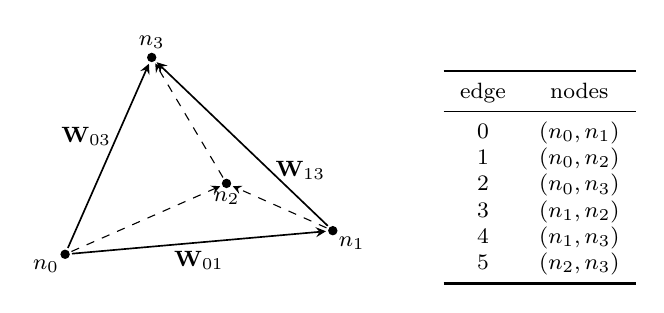
\begin{tikzpicture}[font=\footnotesize,
  sd/.style={line width=0.6pt, ->, >=stealth, shorten >=2.5pt, shorten <=2.5pt},
  hd/.style={line width=0.4pt, dashed, ->, >=stealth, shorten >=2.5pt, shorten <=2.5pt}]
% base as a flattened ellipse seen from above, apex over its centre
\coordinate (n0) at (0.30,0.55);
\coordinate (n1) at (3.70,0.85);
\coordinate (n2) at (2.35,1.45);
\coordinate (n3) at (1.40,3.05);
\draw[sd] (n0) -- (n1);
\draw[hd] (n0) -- (n2);
\draw[sd] (n0) -- (n3);
\draw[hd] (n1) -- (n2);
\draw[sd] (n1) -- (n3);
\draw[hd] (n2) -- (n3);
\foreach \i in {0,1,2,3} \fill (n\i) circle (1.7pt);
\node[below left, inner sep=2pt] at (n0) {$n_0$};
\node[below right, inner sep=2pt] at (n1) {$n_1$};
\node[below, inner sep=3pt] at (n2) {$n_2$};
\node[above, inner sep=3pt] at (n3) {$n_3$};
\node[below, inner sep=3pt] at ($(n0)!0.5!(n1)$) {$\mathbf{W}_{01}$};
\node[left, inner sep=2pt] at ($(n0)!0.6!(n3)$) {$\mathbf{W}_{03}$};
\node[right, inner sep=2pt] at ($(n1)!0.35!(n3)$) {$\mathbf{W}_{13}$};
\begin{scope}[xshift=5.1cm, yshift=0.3cm]
\node[anchor=north west, inner sep=0pt] at (0,2.6) {\begin{tabular}{cc}
\toprule
edge & nodes \\
\midrule
0 & $(n_0, n_1)$ \\
1 & $(n_0, n_2)$ \\
2 & $(n_0, n_3)$ \\
3 & $(n_1, n_2)$ \\
4 & $(n_1, n_3)$ \\
5 & $(n_2, n_3)$ \\
\bottomrule
\end{tabular}};
\end{scope}
\end{tikzpicture}
\caption{The six edge unknowns of a tetrahedron and the local edge table the
code uses. The unknown on an edge is the line integral of \(\mathbf{E}\)
along it. Node indices are sorted on input, so every arrow runs from the
lower to the higher global index and two tetrahedra sharing an edge assign
it the same direction without a sign convention. Edges meeting the rear node
\(n_2\) are dashed.}
\label{fig:tet}
\end{figure}

\begin{derivation}{the element matrices in closed form}
The gradients \(\nabla\lambda\) are constant over a straight tetrahedron, so
the stiffness entry follows immediately from~\eqref{eq:whitney},
\[
S_{ij} = \int_T \frac{1}{\mu_r} (\nabla \times \mathbf{W}_i) \cdot (\nabla \times \mathbf{W}_j)
= \frac{4V}{\mu_r} (\nabla\lambda_a \times \nabla\lambda_b) \cdot (\nabla\lambda_c \times \nabla\lambda_d),
\]
with \(V\) the element volume and \((a,b)\), \((c,d)\) the vertex pairs of
edges \(i\) and \(j\). The mass entry needs only the integrals of products
of barycentric coordinates, which are
\(\int_T \lambda_p \lambda_q = V/10\) for \(p = q\) and \(V/20\) otherwise,
giving the four term expression
\[
M_{ij} = (\nabla\lambda_b \cdot \nabla\lambda_d) I_{ac}
- (\nabla\lambda_b \cdot \nabla\lambda_c) I_{ad}
- (\nabla\lambda_a \cdot \nabla\lambda_d) I_{bc}
+ (\nabla\lambda_a \cdot \nabla\lambda_c) I_{bd}.
\]
No quadrature is needed anywhere in the element loop. The same expression,
with the surface gradients of a triangle and \(I_{pq} = A/6\) or \(A/12\),
gives the face mass matrix used by every boundary condition, so one helper
serves both.
\end{derivation}

\section{Dispersion and mesh density}
\locbar{theory and measurement}{0 lines}{0}{0}

The discrete dispersion error of an edge element of order \(p\) scales as
\((kh)^{2p}\), so the phase a wave accumulates over a length \(L\) carries a
relative error that grows as \(k^{2p+1}\). For the first order elements used
here this means the phase error rises with the cube of frequency at fixed
mesh, and the mesh must be sized by the shortest wavelength in the model.
Table~\ref{tab:order} gives the measured error over the reference line and
fixes the mesh density: ten cells per wavelength give a relative phase error
near one percent, thirty give one part in fifteen hundred.

\begin{table}[H]
\centering
\begin{tabular}{rrr}
\toprule
cells per wavelength & phase error / rad & relative \\
\midrule
30.0 & \(1.63 \times 10^{-3}\) & \(6.48 \times 10^{-4}\) \\
10.0 & \(4.53 \times 10^{-2}\) & \(6.00 \times 10^{-3}\) \\
6.0 & \(2.22 \times 10^{-1}\) & \(1.77 \times 10^{-2}\) \\
3.7 & \(1.04 \times 10^{0}\) & \(5.17 \times 10^{-2}\) \\
\bottomrule
\end{tabular}
\caption{Accumulated phase error of a TEM line against its exact value
\(-k_0 L\). The measured growth per factor three in frequency is \(27.8\),
against \(27\) from the \(k^{3}\) law.}
\label{tab:order}
\end{table}

\begin{fieldnote}{an under-resolved mesh shifts a resonance without failing}
Dispersion error slows the discrete wave, which lengthens the electrical
size of a structure and moves every resonance down. Nothing in the output
marks this: the scattering parameters remain passive, reciprocal and smooth,
the pivot spread and the residual stay small, and the only symptom is that
the answer is wrong. The reference antenna in section~\ref{sec:results}
resonates at \(2.48\) GHz on a mesh graded from \(3\) to \(9\) mm and at
\(2.50\) GHz on the mesh of section~\ref{sec:results}, refined by a factor
of one and a half. Mesh convergence has to be established by
running two densities, since no diagnostic in the solver can substitute for
it.
\end{fieldnote}

\section{The mesh reader and orientation}
\locbar{Gmsh mesh reader}{87 lines, budget 71 to 158}{71}{158}

The Whitney function of an edge depends on which of its two vertices is
called \(a\). Two tetrahedra sharing an edge must agree, or their
contributions cancel instead of adding. The textbook remedy is to give every
global edge a reference direction and to carry a sign through assembly,
excitation and field evaluation.

\begin{decision}{sort the element vertices when reading the mesh}
The mesh reader sorts the four node indices of every tetrahedron and the
three of every triangle into ascending order. Every local edge \((a,b)\)
then satisfies \(a < b\) in global numbering, so all elements agree on the
direction of every shared edge by construction. Assembly, the port excitation integral and the field
export are then all sign free. One line in the reader replaces about ten
sign carrying expressions elsewhere, and a sign error in any of them cancels
contributions instead of adding them, which changes the result without
failing visibly.
\end{decision}

Sorting changes the sign of the Jacobian determinant, which is why the
volume is taken as \(|\det|/6\); the barycentric gradients themselves are
geometric quantities and do not depend on the vertex order.

\section{Materials and the perfectly matched layer}
\locbar{roles, materials, PML tensors}{73 lines, budget 518 to 591}{518}{591}

A material is a relative permittivity with a loss tangent, a relative
permeability, and a conductivity. A perfectly matched layer is not a
material but a coordinate transformation: stretching coordinate \(k\) into
the complex plane by \(s_k = 1 - j a_k\) turns an outgoing wave into a
decaying one without reflecting it. Writing the stretched operator back in
ordinary coordinates turns the stretch into a diagonal tensor applied to
both \(\varepsilon\) and \(\mu\),
\begin{equation}
\Lambda_k = \frac{s_x s_y s_z}{s_k^2},
\qquad
\varepsilon \rightarrow \varepsilon \Lambda,
\qquad
\mu \rightarrow \mu \Lambda .
\label{eq:pml}
\end{equation}
Applying the same tensor to both keeps the wave impedance of the layer equal
to that of the region it terminates, which is what makes it reflectionless
at the continuous level. The code stores \(\Lambda\) alone and multiplies the
resulting mass entry by \(\varepsilon\), which costs one tensor contraction
per element pair instead of two and is what lets conductivity reuse the same
entry.

A first order absorbing boundary is the cheaper alternative: the surface
term of~\eqref{eq:weak} is replaced by \(j k_0 \sqrt{\varepsilon/\mu}\)
times the tangential face mass matrix, which is exact for a plane wave at
normal incidence and degrades with angle. It needs no extra mesh, while a
PML needs a layer of elements. With three cells the PML reflects at
\(-30.7\) dB in the test suite, and a stretch of the same magnitude on all
three axes instead of one costs less than a decibel of that, so a single
shell region serves the faces, edges and corners of a box alike. Against
the extra elements, an absorbing boundary has to stand off a quarter
wavelength or more from a radiator to be accurate at the angles that
matter, while a PML does not: the reference antenna of
section~\ref{sec:results} needs a third of the air height it needed with an
absorbing boundary.

\section{Loss and the frequency decomposition}
\locbar{volume and boundary assembly}{76 lines, budget 651 to 727}{651}{727}

Every entry of the system matrix is a sum of terms with a known dependence
on \(k_0\). The curl stiffness is constant, the mass enters as \(-k_0^2\),
and the boundary terms as \(+j k_0\). Without loss the matrix is a quadratic
polynomial in \(k_0\), so the assembly can run once for an entire sweep. Two
of the three loss mechanisms preserve that form and the third extends it by
one term.

\begin{derivation}{conductivity is a term linear in the wave number}
A conductive region has \(\varepsilon_c = \varepsilon_r - j\sigma/(\omega
\varepsilon_0)\). Substituting into the mass term of~\eqref{eq:weak},
\[
-k_0^2 \varepsilon_c = -k_0^2 \varepsilon_r + j \frac{k_0^2 \sigma}{\omega \varepsilon_0}
= -k_0^2 \varepsilon_r + j k_0 \eta_0 \sigma,
\]
using \(\omega = k_0 c_0\) and \(\eta_0 = 1/(c_0 \varepsilon_0)\). The
conduction current is therefore a term linear in \(k_0\) built from the same
mass matrix, so it needs no new element integral, only a second scaling of
an entry that already exists.
\end{derivation}

\begin{derivation}{the skin effect is a term in the square root of the wave number}
A good conductor is modelled as a surface impedance \(Z_s = (1+j) R_s\) with
\(R_s = \sqrt{\omega \mu_0 / 2\sigma}\). Its contribution to the boundary
term is \(j k_0 \eta_0 / Z_s\) times the face mass matrix. With \(\omega \mu_0
= k_0 \eta_0\),
\[
\frac{j k_0 \eta_0}{(1+j)\sqrt{k_0 \eta_0 / 2\sigma}}
= \sqrt{k_0} \, \frac{j}{1+j} \sqrt{2 \sigma \eta_0}
= \sqrt{k_0} \, \frac{1+j}{2} \sqrt{2 \sigma \eta_0}.
\]
The frequency dependence collapses to \(\sqrt{k_0}\) with a constant
coefficient.
\end{derivation}

\begin{decision}{four coefficients per matrix entry}
Each assembled entry stores four complex numbers, the coefficients against
the basis \(\{1,\, k_0,\, k_0^2,\, \sqrt{k_0}\}\). Evaluating a frequency is
then four multiplications per nonzero. The assembly runs once regardless of how many
frequencies the sweep contains. The cost is three additional complex numbers
per nonzero, against a rebuild of the element loop per frequency.
\end{decision}

\section{Ordering and the direct solve}
\locbar{ordering and sparse \(LDL^T\)}{213 lines, budget 246 to 459}{246}{459}

The system is complex symmetric, not Hermitian: the absorbing boundary and
the port sheets contribute \(j\) times a real symmetric matrix. It is
therefore factored as \(LDL^T\) without conjugation, up-looking, with the
elimination tree and exact column counts computed once in a symbolic pass
and reused for every frequency of the sweep.

\begin{decision}{a direct solver, not an iterative one}
Iterative solvers are the usual choice at this problem size. The gradient
nullspace of the curl-curl operator makes Krylov methods with a diagonal
preconditioner converge slowly, and the preconditioners that work on the
edge space, auxiliary space methods and algebraic multigrid, are larger than
the entire budget. A direct factorization has a predictable cost and no
convergence parameters. The ceiling is memory, at a few tens of thousands of
unknowns.
\end{decision}

Fill is controlled by a geometric nested dissection ordering: split the
unknowns at the median of the longest bounding box axis, take as separator
those vertices of the second half with a neighbour in the first, order both
halves recursively and the separator last. On the reference antenna this
gives \(1.88\) million nonzeros in \(L\) against \(19.1\) million in the
natural order, a factor of ten.

\subsection{Equilibration and refinement}


\begin{figure}[H]
\centering
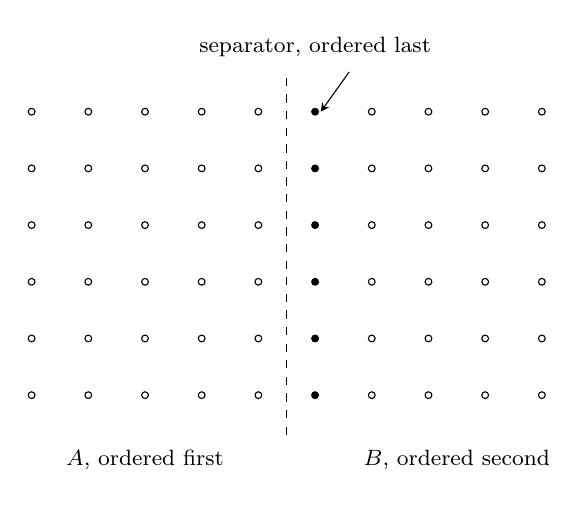
\begin{tikzpicture}[font=\footnotesize, scale=0.72]
\foreach \x in {0,...,9} \foreach \y in {0,...,5} {
  \pgfmathsetmacro{\isep}{ifthenelse(\x==5,1,0)}
  \ifnum\x=5 \fill (\x,\y) circle (2.0pt);
  \else \draw[line width=0.4pt] (\x,\y) circle (1.7pt); \fi
}
\draw[line width=0.5pt, dashed] (4.5,-0.7) -- (4.5,5.7);
\node[below] at (2.0,-0.8) {$A$, ordered first};
\node[below] at (7.5,-0.8) {$B$, ordered second};
\node[above] at (5.0,5.8) {separator, ordered last};
\draw[line width=0.4pt, ->, >=stealth] (5.6,5.7) -- (5.1,5.0);
\end{tikzpicture}
\caption{One level of the geometric nested dissection. The unknowns are
split at the median of the longest bounding box axis. Those on the second
side with a neighbour on the first form the separator and are numbered
after both halves, so no fill can connect \(A\) to \(B\). Both halves are
then split recursively down to blocks of 32.}
\label{fig:nd}
\end{figure}

\subsection{Equilibration and refinement}

Without pivoting an \(LDL^T\) can lose accuracy on an indefinite matrix, and
the curl-curl system is indefinite by construction above the first
resonance. Bunch-Kaufman pivoting is the standard remedy and does not
fit the budget. Two cheaper measures are used instead.

The matrix is first equilibrated symmetrically, \(D A D\) with \(D_{ii} =
|A_{ii}|^{-1/2}\), which puts the rows on a common scale. Figure~\ref{fig:cond}
shows the effect on the spread of the pivots, which the factorization
produces for free and which bounds the condition number from below.

\begin{figure}[H]
\centering
\begin{tikzpicture}
\begin{axis}[bwaxis, width=0.72\textwidth, height=0.36\textwidth,
  xmode=log, ymode=log, xlabel={frequency / Hz},
  ylabel={$\max|D| / \min|D|$}, legend pos=north east]
\addplot[black, thick, mark=*, mark size=1.4pt] table[x=f, y=cond] {data/cond.dat};
\addplot[black, dashed, mark=o, mark size=1.6pt] table[x=f, y=plain] {data/cond.dat};
\legend{equilibrated, as assembled}
\end{axis}
\end{tikzpicture}
\caption{Pivot spread of the reference antenna against frequency. The
\(1/f^2\) branch on the left is the low frequency breakdown of the
curl-curl operator, which loses the mass term that regularizes its
nullspace. The rise on the right sets in once the mesh becomes coarse
against the wavelength. Equilibration gains a factor of about three over the
low frequency branch and about four in the operating band.}
\label{fig:cond}
\end{figure}

Every solve is then followed by one step of iterative refinement against the
unscaled matrix: form \(r = b - Ax\), solve \(A \delta = r\) with the
factorization already in hand, and add. It costs two sparse matrix vector
products and one extra triangular solve, against a factorization that
dominates the runtime by two orders of magnitude, and it lowers the relative
residual by about a factor of four. The residual is then measured rather
than assumed; it and the pivot spread are printed at the end of a run.

\begin{decision}{report the residual instead of trusting the factorization}
A direct solver returns a vector and no measure of how well it solved.
Refinement already forms the residual, so reporting the worst relative
residual over the sweep costs one further matrix vector product per solve.
Conditioning then does not have to be inferred from the mesh and the
frequency.
\end{decision}

\section{Ports and scattering parameters}
\locbar{port geometry, sweep and parameters}{132 lines, budget 629 to 651 and 773 to 883}{629}{883}

A lumped port is a rectangular patch of boundary carrying a sheet impedance
in parallel with an impressed surface current, the Norton equivalent of a
source with internal resistance. Its geometry is read from the mesh: the
height \(h\) is the extent of the patch along the given voltage direction
and the width follows from the total area, \(w = A/h\). The sheet impedance
is then \(Z_s = z_0 w / h\), and the port contributes \(j k_0 \eta_0 / Z_s\)
times the face mass matrix, the same expression as every other boundary
condition.


\begin{figure}[H]
\centering
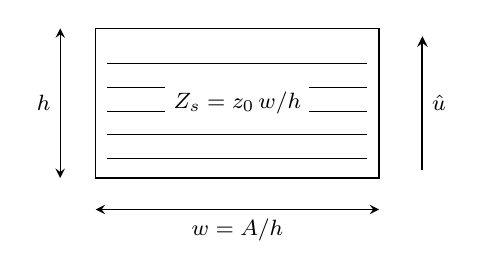
\begin{tikzpicture}[font=\footnotesize, scale=1.0]
\draw[line width=0.5pt] (0,0) rectangle (3.6,1.9);
\foreach \y in {0.25,0.55,...,1.75} \draw[line width=0.25pt] (0.15,\y) -- (3.45,\y);
\draw[line width=0.5pt, <->, >=stealth] (-0.45,0) -- (-0.45,1.9);
\node[left] at (-0.45,0.95) {$h$};
\draw[line width=0.5pt, <->, >=stealth] (0,-0.4) -- (3.6,-0.4);
\node[below] at (1.8,-0.4) {$w = A/h$};
\draw[line width=0.7pt, ->, >=stealth] (4.15,0.1) -- (4.15,1.8);
\node[right] at (4.15,0.95) {$\hat{u}$};
\node at (1.8,0.95) {\colorbox{white}{$Z_s = z_0\, w/h$}};
\end{tikzpicture}
\caption{A lumped port. The patch of boundary triangles carries a sheet
impedance and an impressed surface current. Its height is the extent of the
patch along the given direction \(\hat{u}\) and its width follows from the
total area, so the deck states only \(\hat{u}\) and the reference impedance
\(z_0\).}
\label{fig:port}
\end{figure}

\begin{derivation}{port voltage without the port area}
The port voltage is the mean field along the direction \(\hat{u}\) times the
height,
\[
V = -\frac{h}{A} \int_A \mathbf{E} \cdot \hat{u} \, dA = -\frac{1}{w} \int_A \mathbf{E} \cdot \hat{u} \, dA,
\]
since \(A = wh\). The area cancels, so the port needs to store only its
width. With port \(p\) driven, the scattering matrix follows from
\(S_{qp} = 2 V_q / \sqrt{z_{0p} z_{0q}} - \delta_{qp}\).
\end{derivation}

One factorization serves all ports of a frequency, since only the right hand
side changes. The frequencies of a sweep are independent problems and run on
separate threads, each holding its own factorization, with the thread count
capped by a memory budget rather than by the core count alone.

The impedance and admittance matrices follow from the scattering matrix by
\(Z = D(I+S)(I-S)^{-1}D\) with \(D = \mathrm{diag}\sqrt{z_0}\), which needs a
small dense complex solve, and \(Y = Z^{-1}\), which needs a second. Reading
a port as a coil gives \(L = \mathrm{Im}(Z)/\omega\) and
\(Q = \mathrm{Im}(Z)/\mathrm{Re}(Z)\), the quantities an inductor extraction
reports.

\section{Results}
\label{sec:results}

\subsection{A patch antenna}

The first model is an edge fed microstrip patch antenna on a
\(1.57\) mm substrate of \(\varepsilon_r = 2.2\), \(90\) by
\(100\) mm in plan with \(20\) mm of air above the substrate, terminated
by a perfectly matched layer \(10\) mm thick around the footprint and on
top. The element size follows a distance field on the patch and the feed,
growing from \(2\) mm at the metal to \(5.5\) mm at the outer corners,
which keeps the aspect ratio bounded through the transition out of the
substrate. That gives \(37676\) tetrahedra and \(41468\) unknowns, and a
sweep of 36 frequencies over the resonance takes \(3.7\) s per frequency.

\begin{figure}[H]
\centering
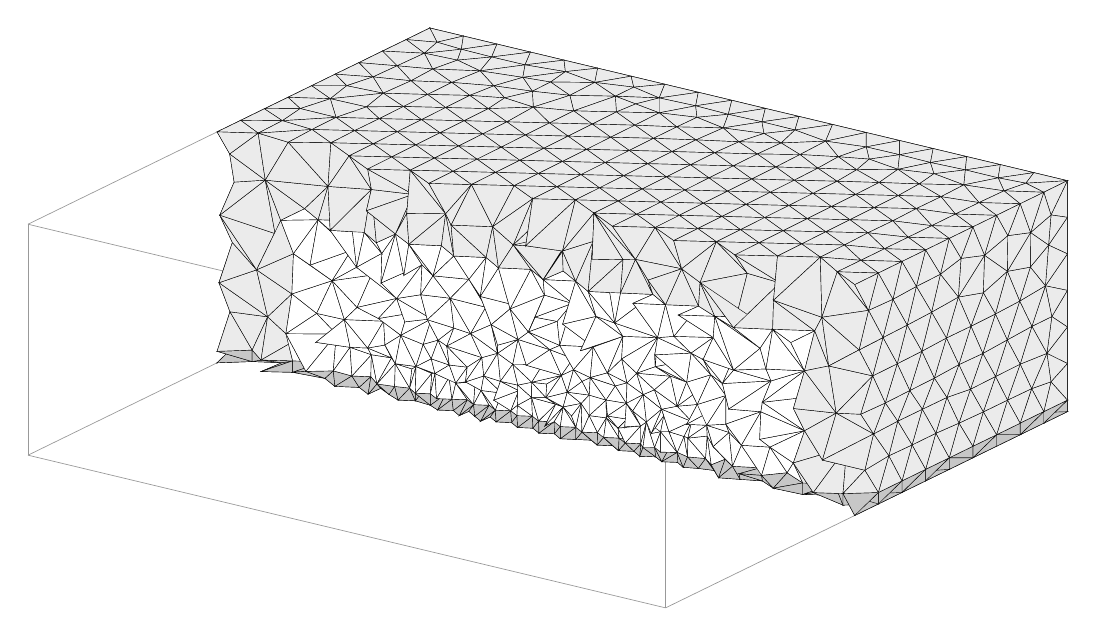
\begin{tikzpicture}
% generated by report/data/gen.py, do not edit
\draw[line width=0.25pt, black!40] (51.03mm,44.32mm) -- (51.03mm,73.64mm);
\draw[line width=0.25pt, black!40] (51.03mm,44.32mm) -- (132.00mm,24.92mm);
\draw[line width=0.25pt, black!40] (51.03mm,44.32mm) -- (0.00mm,19.39mm);
\draw[line width=0.25pt, black!40] (51.03mm,73.64mm) -- (132.00mm,54.25mm);
\draw[line width=0.25pt, black!40] (51.03mm,73.64mm) -- (0.00mm,48.72mm);
\draw[line width=0.25pt, black!40] (132.00mm,24.92mm) -- (132.00mm,54.25mm);
\draw[line width=0.25pt, black!40] (132.00mm,24.92mm) -- (80.97mm,0.00mm);
\draw[line width=0.25pt, black!40] (132.00mm,54.25mm) -- (80.97mm,29.32mm);
\draw[line width=0.25pt, black!40] (0.00mm,19.39mm) -- (0.00mm,48.72mm);
\draw[line width=0.25pt, black!40] (0.00mm,19.39mm) -- (80.97mm,0.00mm);
\draw[line width=0.25pt, black!40] (0.00mm,48.72mm) -- (80.97mm,29.32mm);
\draw[line width=0.25pt, black!40] (80.97mm,0.00mm) -- (80.97mm,29.32mm);
\filldraw[fill=black!22, draw=black, line width=0.15pt] (51.03mm,44.32mm) -- (51.03mm,45.77mm) -- (55.34mm,43.28mm) -- cycle;
\filldraw[fill=black!22, draw=black, line width=0.15pt] (51.03mm,44.32mm) -- (51.03mm,45.77mm) -- (48.03mm,42.85mm) -- cycle;
\filldraw[fill=black!8, draw=black, line width=0.15pt] (51.03mm,45.77mm) -- (51.03mm,50.42mm) -- (54.02mm,48.40mm) -- cycle;
\filldraw[fill=black!22, draw=black, line width=0.15pt] (51.03mm,45.77mm) -- (55.34mm,44.74mm) -- (55.34mm,43.28mm) -- cycle;
\filldraw[fill=black!8, draw=black, line width=0.15pt] (51.03mm,45.77mm) -- (51.03mm,50.42mm) -- (48.93mm,48.10mm) -- cycle;
\filldraw[fill=black!8, draw=black, line width=0.15pt] (51.03mm,45.77mm) -- (55.34mm,44.74mm) -- (54.02mm,48.40mm) -- cycle;
\filldraw[fill=black!22, draw=black, line width=0.15pt] (51.03mm,44.32mm) -- (55.34mm,43.28mm) -- (51.95mm,42.48mm) -- cycle;
\filldraw[fill=black!22, draw=black, line width=0.15pt] (51.03mm,44.32mm) -- (48.03mm,42.85mm) -- (51.95mm,42.48mm) -- cycle;
\filldraw[fill=black!22, draw=black, line width=0.15pt] (51.03mm,45.77mm) -- (48.03mm,42.85mm) -- (48.03mm,44.31mm) -- cycle;
\filldraw[fill=black!8, draw=black, line width=0.15pt] (51.03mm,45.77mm) -- (48.03mm,44.31mm) -- (48.93mm,48.10mm) -- cycle;
\filldraw[fill=black!8, draw=black, line width=0.15pt] (51.03mm,50.42mm) -- (54.89mm,52.33mm) -- (54.02mm,48.40mm) -- cycle;
\filldraw[fill=black!22, draw=black, line width=0.15pt] (55.34mm,44.74mm) -- (55.34mm,43.28mm) -- (59.65mm,42.25mm) -- cycle;
\filldraw[fill=black!8, draw=black, line width=0.15pt] (51.03mm,50.42mm) -- (51.03mm,55.06mm) -- (54.89mm,52.33mm) -- cycle;
\filldraw[fill=black!8, draw=black, line width=0.15pt] (51.03mm,50.42mm) -- (51.03mm,55.06mm) -- (48.57mm,51.54mm) -- cycle;
\filldraw[fill=black!8, draw=black, line width=0.15pt] (51.03mm,50.42mm) -- (48.57mm,51.54mm) -- (48.93mm,48.10mm) -- cycle;
\filldraw[fill=black!8, draw=black, line width=0.15pt] (55.34mm,44.74mm) -- (57.56mm,48.02mm) -- (54.02mm,48.40mm) -- cycle;
\filldraw[fill=black!22, draw=black, line width=0.15pt] (55.34mm,44.74mm) -- (59.66mm,43.71mm) -- (59.65mm,42.25mm) -- cycle;
\filldraw[fill=black!22, draw=black, line width=0.15pt] (55.34mm,43.28mm) -- (54.52mm,41.49mm) -- (51.95mm,42.48mm) -- cycle;
\filldraw[fill=black!8, draw=black, line width=0.15pt] (54.89mm,52.33mm) -- (57.56mm,48.02mm) -- (54.02mm,48.40mm) -- cycle;
\filldraw[fill=black!8, draw=black, line width=0.15pt] (55.34mm,44.74mm) -- (59.66mm,43.71mm) -- (57.56mm,48.02mm) -- cycle;
\filldraw[fill=black!22, draw=black, line width=0.15pt] (55.34mm,43.28mm) -- (59.65mm,42.25mm) -- (54.52mm,41.49mm) -- cycle;
\filldraw[fill=black!8, draw=black, line width=0.15pt] (51.03mm,55.06mm) -- (51.03mm,59.71mm) -- (54.08mm,56.71mm) -- cycle;
\filldraw[fill=black!8, draw=black, line width=0.15pt] (51.03mm,55.06mm) -- (54.89mm,52.33mm) -- (54.08mm,56.71mm) -- cycle;
\filldraw[fill=black!22, draw=black, line width=0.15pt] (48.03mm,42.85mm) -- (45.02mm,41.38mm) -- (48.03mm,44.31mm) -- cycle;
\filldraw[fill=black!8, draw=black, line width=0.15pt] (48.03mm,44.31mm) -- (46.73mm,47.52mm) -- (48.93mm,48.10mm) -- cycle;
\filldraw[fill=black!22, draw=black, line width=0.15pt] (48.03mm,42.85mm) -- (50.08mm,41.24mm) -- (51.95mm,42.48mm) -- cycle;
\filldraw[fill=black!8, draw=black, line width=0.15pt] (51.03mm,55.06mm) -- (51.03mm,59.71mm) -- (48.07mm,56.11mm) -- cycle;
\filldraw[fill=black!8, draw=black, line width=0.15pt] (48.57mm,51.54mm) -- (46.73mm,47.52mm) -- (48.93mm,48.10mm) -- cycle;
\filldraw[fill=black!8, draw=black, line width=0.15pt] (51.03mm,55.06mm) -- (48.57mm,51.54mm) -- (48.07mm,56.11mm) -- cycle;
\filldraw[fill=black!22, draw=black, line width=0.15pt] (59.66mm,43.71mm) -- (59.65mm,42.25mm) -- (63.78mm,41.26mm) -- cycle;
\filldraw[fill=black!22, draw=black, line width=0.15pt] (48.03mm,42.85mm) -- (45.02mm,41.38mm) -- (50.08mm,41.24mm) -- cycle;
\filldraw[fill=black!8, draw=black, line width=0.15pt] (48.03mm,44.31mm) -- (45.02mm,42.84mm) -- (46.73mm,47.52mm) -- cycle;
\filldraw[fill=black!8, draw=black, line width=0.15pt] (54.89mm,52.33mm) -- (59.67mm,51.76mm) -- (57.56mm,48.02mm) -- cycle;
\filldraw[fill=black!22, draw=black, line width=0.15pt] (45.02mm,41.38mm) -- (48.03mm,44.31mm) -- (45.02mm,42.84mm) -- cycle;
\filldraw[fill=black!22, draw=black, line width=0.15pt] (54.52mm,41.49mm) -- (50.08mm,41.24mm) -- (51.95mm,42.48mm) -- cycle;
\filldraw[fill=black!8, draw=black, line width=0.15pt] (59.66mm,43.71mm) -- (61.75mm,47.18mm) -- (57.56mm,48.02mm) -- cycle;
\filldraw[fill=black!8, draw=black, line width=0.15pt] (51.03mm,59.71mm) -- (55.41mm,60.77mm) -- (54.08mm,56.71mm) -- cycle;
\filldraw[fill=black!8, draw=black, line width=0.15pt] (54.89mm,52.33mm) -- (57.70mm,56.23mm) -- (54.08mm,56.71mm) -- cycle;
\filldraw[fill=black!8, draw=black, line width=0.15pt] (51.03mm,59.71mm) -- (51.03mm,64.35mm) -- (55.41mm,60.77mm) -- cycle;
\filldraw[fill=black!8, draw=black, line width=0.15pt] (51.03mm,59.71mm) -- (51.03mm,64.35mm) -- (48.62mm,61.06mm) -- cycle;
\filldraw[fill=black!22, draw=black, line width=0.15pt] (59.66mm,43.71mm) -- (63.79mm,42.72mm) -- (63.78mm,41.26mm) -- cycle;
\filldraw[fill=black!8, draw=black, line width=0.15pt] (51.03mm,59.71mm) -- (48.62mm,61.06mm) -- (48.07mm,56.11mm) -- cycle;
\filldraw[fill=black!8, draw=black, line width=0.15pt] (59.66mm,43.71mm) -- (63.79mm,42.72mm) -- (61.75mm,47.18mm) -- cycle;
\filldraw[fill=black!8, draw=black, line width=0.15pt] (54.89mm,52.33mm) -- (59.67mm,51.76mm) -- (57.70mm,56.23mm) -- cycle;
\filldraw[fill=black!8, draw=black, line width=0.15pt] (61.75mm,47.18mm) -- (59.67mm,51.76mm) -- (57.56mm,48.02mm) -- cycle;
\filldraw[fill=black!22, draw=black, line width=0.15pt] (59.65mm,42.25mm) -- (63.78mm,41.26mm) -- (61.02mm,40.54mm) -- cycle;
\filldraw[fill=black!8, draw=black, line width=0.15pt] (48.57mm,51.54mm) -- (46.73mm,47.52mm) -- (45.83mm,51.16mm) -- cycle;
\filldraw[fill=black!22, draw=black, line width=0.15pt] (59.65mm,42.25mm) -- (57.28mm,40.18mm) -- (54.52mm,41.49mm) -- cycle;
\filldraw[fill=black!8, draw=black, line width=0.15pt] (55.41mm,60.77mm) -- (57.70mm,56.23mm) -- (54.08mm,56.71mm) -- cycle;
\filldraw[fill=black!8, draw=black, line width=0.15pt] (48.57mm,51.54mm) -- (48.07mm,56.11mm) -- (45.83mm,51.16mm) -- cycle;
\filldraw[fill=black!8, draw=black, line width=0.15pt] (51.03mm,64.35mm) -- (51.03mm,69.00mm) -- (54.53mm,65.94mm) -- cycle;
\filldraw[fill=black!8, draw=black, line width=0.15pt] (51.03mm,64.35mm) -- (55.41mm,60.77mm) -- (54.53mm,65.94mm) -- cycle;
\filldraw[fill=black!22, draw=black, line width=0.15pt] (59.65mm,42.25mm) -- (57.28mm,40.18mm) -- (61.02mm,40.54mm) -- cycle;
\filldraw[fill=black!8, draw=black, line width=0.15pt] (51.03mm,64.35mm) -- (51.03mm,69.00mm) -- (48.72mm,65.56mm) -- cycle;
\filldraw[fill=black!8, draw=black, line width=0.15pt] (45.02mm,42.84mm) -- (43.83mm,46.45mm) -- (46.73mm,47.52mm) -- cycle;
\filldraw[fill=black!22, draw=black, line width=0.15pt] (63.79mm,42.72mm) -- (63.78mm,41.26mm) -- (67.61mm,40.35mm) -- cycle;
\filldraw[fill=black!8, draw=black, line width=0.15pt] (51.03mm,64.35mm) -- (48.62mm,61.06mm) -- (48.72mm,65.56mm) -- cycle;
\filldraw[fill=black!22, draw=black, line width=0.15pt] (53.46mm,39.61mm) -- (54.52mm,41.49mm) -- (50.08mm,41.24mm) -- cycle;
\filldraw[fill=black!22, draw=black, line width=0.15pt] (45.02mm,41.38mm) -- (49.06mm,39.71mm) -- (50.08mm,41.24mm) -- cycle;
\filldraw[fill=black!22, draw=black, line width=0.15pt] (45.02mm,41.38mm) -- (45.02mm,42.84mm) -- (42.02mm,41.38mm) -- cycle;
\filldraw[fill=black!8, draw=black, line width=0.15pt] (63.79mm,42.72mm) -- (61.75mm,47.18mm) -- (65.72mm,45.99mm) -- cycle;
\filldraw[fill=black!8, draw=black, line width=0.15pt] (43.83mm,46.45mm) -- (46.73mm,47.52mm) -- (45.83mm,51.16mm) -- cycle;
\filldraw[fill=black!8, draw=black, line width=0.15pt] (61.75mm,47.18mm) -- (63.93mm,50.61mm) -- (59.67mm,51.76mm) -- cycle;
\filldraw[fill=black!8, draw=black, line width=0.15pt] (62.06mm,55.36mm) -- (59.67mm,51.76mm) -- (57.70mm,56.23mm) -- cycle;
\filldraw[fill=black!8, draw=black, line width=0.15pt] (55.41mm,60.77mm) -- (57.70mm,56.23mm) -- (60.15mm,59.15mm) -- cycle;
\filldraw[fill=black!8, draw=black, line width=0.15pt] (51.03mm,69.00mm) -- (54.53mm,65.94mm) -- (54.00mm,69.59mm) -- cycle;
\filldraw[fill=black!8, draw=black, line width=0.15pt] (51.03mm,73.64mm) -- (51.03mm,69.00mm) -- (54.00mm,69.59mm) -- cycle;
\filldraw[fill=black!8, draw=black, line width=0.15pt] (48.62mm,61.06mm) -- (48.07mm,56.11mm) -- (46.23mm,58.81mm) -- cycle;
\filldraw[fill=black!22, draw=black, line width=0.15pt] (63.79mm,42.72mm) -- (67.62mm,41.80mm) -- (67.61mm,40.35mm) -- cycle;
\filldraw[fill=black!22, draw=black, line width=0.15pt] (63.78mm,41.26mm) -- (63.94mm,39.75mm) -- (61.02mm,40.54mm) -- cycle;
\filldraw[fill=black!8, draw=black, line width=0.15pt] (51.03mm,73.64mm) -- (51.03mm,69.00mm) -- (49.10mm,69.59mm) -- cycle;
\filldraw[fill=black!22, draw=black, line width=0.15pt] (63.78mm,41.26mm) -- (67.61mm,40.35mm) -- (63.94mm,39.75mm) -- cycle;
\filldraw[fill=black!8, draw=black, line width=0.15pt] (63.79mm,42.72mm) -- (67.62mm,41.80mm) -- (65.72mm,45.99mm) -- cycle;
\filldraw[fill=black!22, draw=black, line width=0.15pt] (53.46mm,39.61mm) -- (57.28mm,40.18mm) -- (54.52mm,41.49mm) -- cycle;
\filldraw[fill=black!8, draw=black, line width=0.15pt] (51.03mm,69.00mm) -- (48.72mm,65.56mm) -- (49.10mm,69.59mm) -- cycle;
\filldraw[fill=black!8, draw=black, line width=0.15pt] (61.75mm,47.18mm) -- (65.72mm,45.99mm) -- (63.93mm,50.61mm) -- cycle;
\filldraw[fill=black!8, draw=black, line width=0.15pt] (44.83mm,55.01mm) -- (48.07mm,56.11mm) -- (45.83mm,51.16mm) -- cycle;
\filldraw[fill=black!8, draw=black, line width=0.15pt] (55.41mm,60.77mm) -- (58.79mm,63.81mm) -- (54.53mm,65.94mm) -- cycle;
\filldraw[fill=black!22, draw=black, line width=0.15pt] (45.02mm,41.38mm) -- (42.02mm,39.92mm) -- (42.02mm,41.38mm) -- cycle;
\filldraw[fill=black!8, draw=black, line width=0.15pt] (45.02mm,42.84mm) -- (42.02mm,41.38mm) -- (43.83mm,46.45mm) -- cycle;
\filldraw[fill=black!22, draw=black, line width=0.15pt] (45.02mm,41.38mm) -- (42.02mm,39.92mm) -- (45.29mm,39.55mm) -- cycle;
\filldraw[fill=black!8, draw=black, line width=0.15pt] (63.93mm,50.61mm) -- (62.06mm,55.36mm) -- (59.67mm,51.76mm) -- cycle;
\filldraw[fill=black!8, draw=black, line width=0.15pt] (62.06mm,55.36mm) -- (57.70mm,56.23mm) -- (60.15mm,59.15mm) -- cycle;
\filldraw[fill=black!22, draw=black, line width=0.15pt] (45.02mm,41.38mm) -- (49.06mm,39.71mm) -- (45.29mm,39.55mm) -- cycle;
\filldraw[fill=black!22, draw=black, line width=0.15pt] (53.46mm,39.61mm) -- (49.06mm,39.71mm) -- (50.08mm,41.24mm) -- cycle;
\filldraw[fill=black!8, draw=black, line width=0.15pt] (55.41mm,60.77mm) -- (58.79mm,63.81mm) -- (60.15mm,59.15mm) -- cycle;
\filldraw[fill=black!8, draw=black, line width=0.15pt] (44.83mm,55.01mm) -- (48.07mm,56.11mm) -- (46.23mm,58.81mm) -- cycle;
\filldraw[fill=black!8, draw=black, line width=0.15pt] (48.62mm,61.06mm) -- (48.72mm,65.56mm) -- (46.23mm,62.79mm) -- cycle;
\filldraw[fill=black!8, draw=black, line width=0.15pt] (57.40mm,68.25mm) -- (54.53mm,65.94mm) -- (54.00mm,69.59mm) -- cycle;
\filldraw[fill=black!8, draw=black, line width=0.15pt] (51.03mm,73.64mm) -- (55.29mm,72.62mm) -- (54.00mm,69.59mm) -- cycle;
\filldraw[fill=black!22, draw=black, line width=0.15pt] (67.62mm,41.80mm) -- (67.61mm,40.35mm) -- (71.20mm,39.48mm) -- cycle;
\filldraw[fill=black!22, draw=black, line width=0.15pt] (57.28mm,40.18mm) -- (60.46mm,39.25mm) -- (61.02mm,40.54mm) -- cycle;
\filldraw[fill=black!8, draw=black, line width=0.15pt] (48.62mm,61.06mm) -- (46.23mm,62.79mm) -- (46.23mm,58.81mm) -- cycle;
\filldraw[fill=black!8, draw=black, line width=0.15pt] (43.83mm,46.45mm) -- (42.93mm,50.36mm) -- (45.83mm,51.16mm) -- cycle;
\filldraw[fill=black!8, draw=black, line width=0.15pt] (57.40mm,68.25mm) -- (58.79mm,63.81mm) -- (54.53mm,65.94mm) -- cycle;
\filldraw[fill=black!22, draw=black, line width=0.15pt] (60.46mm,39.25mm) -- (63.94mm,39.75mm) -- (61.02mm,40.54mm) -- cycle;
\filldraw[fill=black!8, draw=black, line width=0.15pt] (67.62mm,41.80mm) -- (65.72mm,45.99mm) -- (69.61mm,45.07mm) -- cycle;
\filldraw[fill=black!8, draw=black, line width=0.15pt] (51.03mm,73.64mm) -- (48.03mm,72.17mm) -- (49.10mm,69.59mm) -- cycle;
\filldraw[fill=black!8, draw=black, line width=0.15pt] (65.72mm,45.99mm) -- (63.93mm,50.61mm) -- (67.96mm,49.38mm) -- cycle;
\filldraw[fill=black!8, draw=black, line width=0.15pt] (44.83mm,55.01mm) -- (42.93mm,50.36mm) -- (45.83mm,51.16mm) -- cycle;
\filldraw[fill=black!8, draw=black, line width=0.15pt] (55.29mm,72.62mm) -- (57.40mm,68.25mm) -- (54.00mm,69.59mm) -- cycle;
\filldraw[fill=black!8, draw=black, line width=0.15pt] (46.70mm,67.58mm) -- (48.72mm,65.56mm) -- (49.10mm,69.59mm) -- cycle;
\filldraw[fill=black!22, draw=black, line width=0.15pt] (67.62mm,41.80mm) -- (71.21mm,40.94mm) -- (71.20mm,39.48mm) -- cycle;
\filldraw[fill=black!22, draw=black, line width=0.15pt] (67.61mm,40.35mm) -- (67.41mm,38.69mm) -- (63.94mm,39.75mm) -- cycle;
\filldraw[fill=black!8, draw=black, line width=0.15pt] (63.93mm,50.61mm) -- (66.20mm,53.85mm) -- (62.06mm,55.36mm) -- cycle;
\filldraw[fill=black!8, draw=black, line width=0.15pt] (67.62mm,41.80mm) -- (71.21mm,40.94mm) -- (69.61mm,45.07mm) -- cycle;
\filldraw[fill=black!8, draw=black, line width=0.15pt] (62.06mm,55.36mm) -- (64.45mm,57.98mm) -- (60.15mm,59.15mm) -- cycle;
\filldraw[fill=black!22, draw=black, line width=0.15pt] (53.46mm,39.61mm) -- (57.01mm,38.76mm) -- (57.28mm,40.18mm) -- cycle;
\filldraw[fill=black!22, draw=black, line width=0.15pt] (67.61mm,40.35mm) -- (71.20mm,39.48mm) -- (67.41mm,38.69mm) -- cycle;
\filldraw[fill=black!8, draw=black, line width=0.15pt] (51.03mm,73.64mm) -- (55.29mm,72.62mm) -- (51.95mm,71.84mm) -- cycle;
\filldraw[fill=black!8, draw=black, line width=0.15pt] (42.02mm,41.38mm) -- (43.83mm,46.45mm) -- (40.88mm,45.02mm) -- cycle;
\filldraw[fill=black!8, draw=black, line width=0.15pt] (65.72mm,45.99mm) -- (67.96mm,49.38mm) -- (69.61mm,45.07mm) -- cycle;
\filldraw[fill=black!8, draw=black, line width=0.15pt] (46.70mm,67.58mm) -- (48.72mm,65.56mm) -- (46.23mm,62.79mm) -- cycle;
\filldraw[fill=black!22, draw=black, line width=0.15pt] (57.01mm,38.76mm) -- (57.28mm,40.18mm) -- (60.46mm,39.25mm) -- cycle;
\filldraw[fill=black!8, draw=black, line width=0.15pt] (58.79mm,63.81mm) -- (63.02mm,62.48mm) -- (60.15mm,59.15mm) -- cycle;
\filldraw[fill=black!22, draw=black, line width=0.15pt] (42.02mm,39.92mm) -- (39.02mm,38.45mm) -- (42.02mm,41.38mm) -- cycle;
\filldraw[fill=black!8, draw=black, line width=0.15pt] (51.03mm,73.64mm) -- (48.03mm,72.17mm) -- (51.95mm,71.84mm) -- cycle;
\filldraw[fill=black!8, draw=black, line width=0.15pt] (63.93mm,50.61mm) -- (67.96mm,49.38mm) -- (66.20mm,53.85mm) -- cycle;
\filldraw[fill=black!22, draw=black, line width=0.15pt] (42.02mm,39.92mm) -- (43.39mm,38.36mm) -- (45.29mm,39.55mm) -- cycle;
\filldraw[fill=black!8, draw=black, line width=0.15pt] (48.03mm,72.17mm) -- (46.70mm,67.58mm) -- (49.10mm,69.59mm) -- cycle;
\filldraw[fill=black!8, draw=black, line width=0.15pt] (43.83mm,46.45mm) -- (40.88mm,45.02mm) -- (42.93mm,50.36mm) -- cycle;
\filldraw[fill=black!8, draw=black, line width=0.15pt] (66.20mm,53.85mm) -- (62.06mm,55.36mm) -- (64.45mm,57.98mm) -- cycle;
\filldraw[fill=black!22, draw=black, line width=0.15pt] (53.46mm,39.61mm) -- (50.85mm,38.34mm) -- (49.06mm,39.71mm) -- cycle;
\filldraw[fill=black!22, draw=black, line width=0.15pt] (49.06mm,39.71mm) -- (46.93mm,38.35mm) -- (45.29mm,39.55mm) -- cycle;
\filldraw[fill=black!8, draw=black, line width=0.15pt] (57.40mm,68.25mm) -- (61.67mm,66.87mm) -- (58.79mm,63.81mm) -- cycle;
\filldraw[fill=black!22, draw=black, line width=0.15pt] (63.34mm,38.47mm) -- (60.46mm,39.25mm) -- (63.94mm,39.75mm) -- cycle;
\filldraw[fill=black!22, draw=black, line width=0.15pt] (71.21mm,40.94mm) -- (71.20mm,39.48mm) -- (74.65mm,38.66mm) -- cycle;
\filldraw[fill=black!8, draw=black, line width=0.15pt] (63.02mm,62.48mm) -- (64.45mm,57.98mm) -- (60.15mm,59.15mm) -- cycle;
\filldraw[fill=black!8, draw=black, line width=0.15pt] (43.39mm,59.09mm) -- (44.83mm,55.01mm) -- (46.23mm,58.81mm) -- cycle;
\filldraw[fill=black!8, draw=black, line width=0.15pt] (55.29mm,72.62mm) -- (59.55mm,71.60mm) -- (57.40mm,68.25mm) -- cycle;
\filldraw[fill=black!8, draw=black, line width=0.15pt] (43.39mm,59.09mm) -- (46.23mm,62.79mm) -- (46.23mm,58.81mm) -- cycle;
\filldraw[fill=black!22, draw=black, line width=0.15pt] (63.34mm,38.47mm) -- (67.41mm,38.69mm) -- (63.94mm,39.75mm) -- cycle;
\filldraw[fill=black!8, draw=black, line width=0.15pt] (71.21mm,40.94mm) -- (73.04mm,43.95mm) -- (69.61mm,45.07mm) -- cycle;
\filldraw[fill=black!22, draw=black, line width=0.15pt] (42.02mm,39.92mm) -- (39.02mm,38.45mm) -- (43.39mm,38.36mm) -- cycle;
\filldraw[fill=black!8, draw=black, line width=0.15pt] (61.67mm,66.87mm) -- (58.79mm,63.81mm) -- (63.02mm,62.48mm) -- cycle;
\filldraw[fill=black!8, draw=black, line width=0.15pt] (42.02mm,41.38mm) -- (39.02mm,39.91mm) -- (40.88mm,45.02mm) -- cycle;
\filldraw[fill=black!22, draw=black, line width=0.15pt] (53.46mm,39.61mm) -- (57.01mm,38.76mm) -- (54.19mm,38.20mm) -- cycle;
\filldraw[fill=black!22, draw=black, line width=0.15pt] (39.02mm,38.45mm) -- (42.02mm,41.38mm) -- (39.02mm,39.91mm) -- cycle;
\filldraw[fill=black!22, draw=black, line width=0.15pt] (71.21mm,40.94mm) -- (74.66mm,40.11mm) -- (74.65mm,38.66mm) -- cycle;
\filldraw[fill=black!22, draw=black, line width=0.15pt] (50.85mm,38.34mm) -- (49.06mm,39.71mm) -- (46.93mm,38.35mm) -- cycle;
\filldraw[fill=black!8, draw=black, line width=0.15pt] (67.96mm,49.38mm) -- (69.61mm,45.07mm) -- (71.82mm,48.26mm) -- cycle;
\filldraw[fill=black!8, draw=black, line width=0.15pt] (41.54mm,53.75mm) -- (44.83mm,55.01mm) -- (42.93mm,50.36mm) -- cycle;
\filldraw[fill=black!22, draw=black, line width=0.15pt] (43.39mm,38.36mm) -- (46.93mm,38.35mm) -- (45.29mm,39.55mm) -- cycle;
\filldraw[fill=black!8, draw=black, line width=0.15pt] (59.55mm,71.60mm) -- (57.40mm,68.25mm) -- (61.67mm,66.87mm) -- cycle;
\filldraw[fill=black!22, draw=black, line width=0.15pt] (53.46mm,39.61mm) -- (50.85mm,38.34mm) -- (54.19mm,38.20mm) -- cycle;
\filldraw[fill=black!8, draw=black, line width=0.15pt] (71.21mm,40.94mm) -- (74.66mm,40.11mm) -- (73.04mm,43.95mm) -- cycle;
\filldraw[fill=black!22, draw=black, line width=0.15pt] (71.20mm,39.48mm) -- (71.19mm,37.95mm) -- (67.41mm,38.69mm) -- cycle;
\filldraw[fill=black!22, draw=black, line width=0.15pt] (71.20mm,39.48mm) -- (74.65mm,38.66mm) -- (71.19mm,37.95mm) -- cycle;
\filldraw[fill=black!22, draw=black, line width=0.15pt] (57.01mm,38.76mm) -- (60.21mm,37.99mm) -- (60.46mm,39.25mm) -- cycle;
\filldraw[fill=black!8, draw=black, line width=0.15pt] (67.96mm,49.38mm) -- (66.20mm,53.85mm) -- (70.31mm,52.68mm) -- cycle;
\filldraw[fill=black!8, draw=black, line width=0.15pt] (55.29mm,72.62mm) -- (55.03mm,70.94mm) -- (51.95mm,71.84mm) -- cycle;
\filldraw[fill=black!8, draw=black, line width=0.15pt] (73.04mm,43.95mm) -- (69.61mm,45.07mm) -- (71.82mm,48.26mm) -- cycle;
\filldraw[fill=black!22, draw=black, line width=0.15pt] (60.21mm,37.99mm) -- (63.34mm,38.47mm) -- (60.46mm,39.25mm) -- cycle;
\filldraw[fill=black!8, draw=black, line width=0.15pt] (66.20mm,53.85mm) -- (68.63mm,57.08mm) -- (64.45mm,57.98mm) -- cycle;
\filldraw[fill=black!8, draw=black, line width=0.15pt] (55.29mm,72.62mm) -- (59.55mm,71.60mm) -- (55.03mm,70.94mm) -- cycle;
\filldraw[fill=black!8, draw=black, line width=0.15pt] (46.70mm,67.58mm) -- (43.59mm,64.91mm) -- (46.23mm,62.79mm) -- cycle;
\filldraw[fill=black!8, draw=black, line width=0.15pt] (41.54mm,53.75mm) -- (43.39mm,59.09mm) -- (44.83mm,55.01mm) -- cycle;
\filldraw[fill=black!8, draw=black, line width=0.15pt] (48.03mm,72.17mm) -- (45.02mm,70.71mm) -- (46.70mm,67.58mm) -- cycle;
\filldraw[fill=black!8, draw=black, line width=0.15pt] (67.96mm,49.38mm) -- (70.31mm,52.68mm) -- (71.82mm,48.26mm) -- cycle;
\filldraw[fill=black!8, draw=black, line width=0.15pt] (63.02mm,62.48mm) -- (64.45mm,57.98mm) -- (67.18mm,61.52mm) -- cycle;
\filldraw[fill=black!8, draw=black, line width=0.15pt] (39.65mm,48.50mm) -- (40.88mm,45.02mm) -- (42.93mm,50.36mm) -- cycle;
\filldraw[fill=black!22, draw=black, line width=0.15pt] (74.66mm,40.11mm) -- (74.65mm,38.66mm) -- (78.04mm,37.85mm) -- cycle;
\filldraw[fill=black!8, draw=black, line width=0.15pt] (43.39mm,59.09mm) -- (43.59mm,64.91mm) -- (46.23mm,62.79mm) -- cycle;
\filldraw[fill=black!8, draw=black, line width=0.15pt] (48.03mm,72.17mm) -- (50.34mm,70.44mm) -- (51.95mm,71.84mm) -- cycle;
\filldraw[fill=black!22, draw=black, line width=0.15pt] (63.34mm,38.47mm) -- (67.41mm,38.69mm) -- (65.62mm,37.64mm) -- cycle;
\filldraw[fill=black!8, draw=black, line width=0.15pt] (66.20mm,53.85mm) -- (70.31mm,52.68mm) -- (68.63mm,57.08mm) -- cycle;
\filldraw[fill=black!8, draw=black, line width=0.15pt] (65.82mm,65.96mm) -- (61.67mm,66.87mm) -- (63.02mm,62.48mm) -- cycle;
\filldraw[fill=black!22, draw=black, line width=0.15pt] (57.01mm,38.76mm) -- (56.90mm,37.53mm) -- (54.19mm,38.20mm) -- cycle;
\filldraw[fill=black!8, draw=black, line width=0.15pt] (74.66mm,40.11mm) -- (73.04mm,43.95mm) -- (76.53mm,43.03mm) -- cycle;
\filldraw[fill=black!8, draw=black, line width=0.15pt] (68.63mm,57.08mm) -- (64.45mm,57.98mm) -- (67.18mm,61.52mm) -- cycle;
\filldraw[fill=black!8, draw=black, line width=0.15pt] (41.54mm,53.75mm) -- (39.65mm,48.50mm) -- (42.93mm,50.36mm) -- cycle;
\filldraw[fill=black!22, draw=black, line width=0.15pt] (57.01mm,38.76mm) -- (60.21mm,37.99mm) -- (56.90mm,37.53mm) -- cycle;
\filldraw[fill=black!8, draw=black, line width=0.15pt] (59.55mm,71.60mm) -- (63.81mm,70.58mm) -- (61.67mm,66.87mm) -- cycle;
\filldraw[fill=black!22, draw=black, line width=0.15pt] (74.66mm,40.11mm) -- (78.05mm,39.30mm) -- (78.04mm,37.85mm) -- cycle;
\filldraw[fill=black!8, draw=black, line width=0.15pt] (39.02mm,39.91mm) -- (37.69mm,43.27mm) -- (40.88mm,45.02mm) -- cycle;
\filldraw[fill=black!22, draw=black, line width=0.15pt] (39.02mm,38.45mm) -- (43.39mm,38.36mm) -- (40.21mm,37.13mm) -- cycle;
\filldraw[fill=black!22, draw=black, line width=0.15pt] (74.65mm,38.66mm) -- (74.26mm,37.24mm) -- (71.19mm,37.95mm) -- cycle;
\filldraw[fill=black!22, draw=black, line width=0.15pt] (43.39mm,38.36mm) -- (44.49mm,37.12mm) -- (46.93mm,38.35mm) -- cycle;
\filldraw[fill=black!8, draw=black, line width=0.15pt] (73.04mm,43.95mm) -- (75.67mm,47.08mm) -- (71.82mm,48.26mm) -- cycle;
\filldraw[fill=black!8, draw=black, line width=0.15pt] (45.02mm,70.71mm) -- (46.70mm,67.58mm) -- (43.59mm,64.91mm) -- cycle;
\filldraw[fill=black!22, draw=black, line width=0.15pt] (50.85mm,38.34mm) -- (48.34mm,37.11mm) -- (46.93mm,38.35mm) -- cycle;
\filldraw[fill=black!22, draw=black, line width=0.15pt] (60.21mm,37.99mm) -- (63.10mm,37.30mm) -- (63.34mm,38.47mm) -- cycle;
\filldraw[fill=black!8, draw=black, line width=0.15pt] (65.82mm,65.96mm) -- (63.02mm,62.48mm) -- (67.18mm,61.52mm) -- cycle;
\filldraw[fill=black!22, draw=black, line width=0.15pt] (74.65mm,38.66mm) -- (78.04mm,37.85mm) -- (74.26mm,37.24mm) -- cycle;
\filldraw[fill=black!22, draw=black, line width=0.15pt] (68.49mm,37.08mm) -- (71.19mm,37.95mm) -- (67.41mm,38.69mm) -- cycle;
\filldraw[fill=black!22, draw=black, line width=0.15pt] (39.02mm,38.45mm) -- (36.02mm,36.99mm) -- (39.02mm,39.91mm) -- cycle;
\filldraw[fill=black!8, draw=black, line width=0.15pt] (48.03mm,72.17mm) -- (45.02mm,70.71mm) -- (50.34mm,70.44mm) -- cycle;
\filldraw[fill=black!8, draw=black, line width=0.15pt] (74.66mm,40.11mm) -- (78.05mm,39.30mm) -- (76.53mm,43.03mm) -- cycle;
\filldraw[fill=black!8, draw=black, line width=0.15pt] (50.34mm,70.44mm) -- (55.03mm,70.94mm) -- (51.95mm,71.84mm) -- cycle;
\filldraw[fill=black!22, draw=black, line width=0.15pt] (50.85mm,38.34mm) -- (53.04mm,37.02mm) -- (54.19mm,38.20mm) -- cycle;
\filldraw[fill=black!22, draw=black, line width=0.15pt] (68.49mm,37.08mm) -- (67.41mm,38.69mm) -- (65.62mm,37.64mm) -- cycle;
\filldraw[fill=black!22, draw=black, line width=0.15pt] (63.10mm,37.30mm) -- (63.34mm,38.47mm) -- (65.62mm,37.64mm) -- cycle;
\filldraw[fill=black!8, draw=black, line width=0.15pt] (63.81mm,70.58mm) -- (65.82mm,65.96mm) -- (61.67mm,66.87mm) -- cycle;
\filldraw[fill=black!8, draw=black, line width=0.15pt] (73.04mm,43.95mm) -- (75.67mm,47.08mm) -- (76.53mm,43.03mm) -- cycle;
\filldraw[fill=black!8, draw=black, line width=0.15pt] (70.31mm,52.68mm) -- (74.37mm,51.40mm) -- (71.82mm,48.26mm) -- cycle;
\filldraw[fill=black!8, draw=black, line width=0.15pt] (39.65mm,48.50mm) -- (37.69mm,43.27mm) -- (40.88mm,45.02mm) -- cycle;
\filldraw[fill=black!8, draw=black, line width=0.15pt] (59.55mm,71.60mm) -- (58.88mm,69.96mm) -- (55.03mm,70.94mm) -- cycle;
\filldraw[fill=black!22, draw=black, line width=0.15pt] (53.04mm,37.02mm) -- (56.90mm,37.53mm) -- (54.19mm,38.20mm) -- cycle;
\filldraw[fill=black!8, draw=black, line width=0.15pt] (70.31mm,52.68mm) -- (68.63mm,57.08mm) -- (72.65mm,55.92mm) -- cycle;
\filldraw[fill=black!22, draw=black, line width=0.15pt] (43.39mm,38.36mm) -- (44.49mm,37.12mm) -- (40.21mm,37.13mm) -- cycle;
\filldraw[fill=black!22, draw=black, line width=0.15pt] (48.34mm,37.11mm) -- (44.49mm,37.12mm) -- (46.93mm,38.35mm) -- cycle;
\filldraw[fill=black!22, draw=black, line width=0.15pt] (39.02mm,38.45mm) -- (36.02mm,36.99mm) -- (40.21mm,37.13mm) -- cycle;
\filldraw[fill=black!22, draw=black, line width=0.15pt] (78.05mm,39.30mm) -- (78.04mm,37.85mm) -- (81.42mm,37.04mm) -- cycle;
\filldraw[fill=black!8, draw=black, line width=0.15pt] (59.55mm,71.60mm) -- (63.81mm,70.58mm) -- (58.88mm,69.96mm) -- cycle;
\filldraw[fill=black!8, draw=black, line width=0.15pt] (43.39mm,59.09mm) -- (43.59mm,64.91mm) -- (41.60mm,61.19mm) -- cycle;
\filldraw[fill=black!8, draw=black, line width=0.15pt] (40.02mm,57.25mm) -- (41.54mm,53.75mm) -- (43.39mm,59.09mm) -- cycle;
\filldraw[fill=black!8, draw=black, line width=0.15pt] (74.37mm,51.40mm) -- (75.67mm,47.08mm) -- (71.82mm,48.26mm) -- cycle;
\filldraw[fill=black!22, draw=black, line width=0.15pt] (50.85mm,38.34mm) -- (48.34mm,37.11mm) -- (53.04mm,37.02mm) -- cycle;
\filldraw[fill=black!22, draw=black, line width=0.15pt] (60.21mm,37.99mm) -- (60.05mm,36.88mm) -- (56.90mm,37.53mm) -- cycle;
\filldraw[fill=black!8, draw=black, line width=0.15pt] (68.63mm,57.08mm) -- (71.23mm,60.52mm) -- (67.18mm,61.52mm) -- cycle;
\filldraw[fill=black!22, draw=black, line width=0.15pt] (60.21mm,37.99mm) -- (63.10mm,37.30mm) -- (60.05mm,36.88mm) -- cycle;
\filldraw[fill=black!8, draw=black, line width=0.15pt] (39.02mm,39.91mm) -- (36.02mm,38.44mm) -- (37.69mm,43.27mm) -- cycle;
\filldraw[fill=black!8, draw=black, line width=0.15pt] (78.05mm,39.30mm) -- (76.53mm,43.03mm) -- (79.77mm,41.60mm) -- cycle;
\filldraw[fill=black!22, draw=black, line width=0.15pt] (36.02mm,36.99mm) -- (39.02mm,39.91mm) -- (36.02mm,38.44mm) -- cycle;
\filldraw[fill=black!8, draw=black, line width=0.15pt] (70.31mm,52.68mm) -- (72.65mm,55.92mm) -- (74.37mm,51.40mm) -- cycle;
\filldraw[fill=black!22, draw=black, line width=0.15pt] (74.26mm,37.24mm) -- (71.19mm,37.95mm) -- (71.01mm,36.62mm) -- cycle;
\filldraw[fill=black!22, draw=black, line width=0.15pt] (68.49mm,37.08mm) -- (71.19mm,37.95mm) -- (71.01mm,36.62mm) -- cycle;
\filldraw[fill=black!8, draw=black, line width=0.15pt] (38.43mm,52.18mm) -- (41.54mm,53.75mm) -- (39.65mm,48.50mm) -- cycle;
\filldraw[fill=black!22, draw=black, line width=0.15pt] (63.10mm,37.30mm) -- (65.77mm,36.66mm) -- (65.62mm,37.64mm) -- cycle;
\filldraw[fill=black!22, draw=black, line width=0.15pt] (78.04mm,37.85mm) -- (74.26mm,37.24mm) -- (77.59mm,36.51mm) -- cycle;
\filldraw[fill=black!8, draw=black, line width=0.15pt] (65.82mm,65.96mm) -- (69.92mm,65.07mm) -- (67.18mm,61.52mm) -- cycle;
\filldraw[fill=black!22, draw=black, line width=0.15pt] (78.05mm,39.30mm) -- (81.43mm,38.49mm) -- (81.42mm,37.04mm) -- cycle;
\filldraw[fill=black!8, draw=black, line width=0.15pt] (40.02mm,57.25mm) -- (43.39mm,59.09mm) -- (41.60mm,61.19mm) -- cycle;
\filldraw[fill=black!8, draw=black, line width=0.15pt] (68.63mm,57.08mm) -- (72.65mm,55.92mm) -- (71.23mm,60.52mm) -- cycle;
\filldraw[fill=black!22, draw=black, line width=0.15pt] (78.04mm,37.85mm) -- (81.42mm,37.04mm) -- (77.59mm,36.51mm) -- cycle;
\filldraw[fill=black!22, draw=black, line width=0.15pt] (65.77mm,36.66mm) -- (68.49mm,37.08mm) -- (65.62mm,37.64mm) -- cycle;
\filldraw[fill=black!8, draw=black, line width=0.15pt] (78.05mm,39.30mm) -- (81.43mm,38.49mm) -- (79.77mm,41.60mm) -- cycle;
\filldraw[fill=black!8, draw=black, line width=0.15pt] (50.34mm,70.44mm) -- (55.03mm,70.94mm) -- (54.54mm,69.56mm) -- cycle;
\filldraw[fill=black!8, draw=black, line width=0.15pt] (63.81mm,70.58mm) -- (68.07mm,69.56mm) -- (65.82mm,65.96mm) -- cycle;
\filldraw[fill=black!8, draw=black, line width=0.15pt] (75.67mm,47.08mm) -- (79.87mm,45.70mm) -- (76.53mm,43.03mm) -- cycle;
\filldraw[fill=black!8, draw=black, line width=0.15pt] (45.02mm,70.71mm) -- (42.02mm,69.24mm) -- (43.59mm,64.91mm) -- cycle;
\filldraw[fill=black!22, draw=black, line width=0.15pt] (53.04mm,37.02mm) -- (56.90mm,37.53mm) -- (56.96mm,36.39mm) -- cycle;
\filldraw[fill=black!8, draw=black, line width=0.15pt] (58.88mm,69.96mm) -- (55.03mm,70.94mm) -- (54.54mm,69.56mm) -- cycle;
\filldraw[fill=black!8, draw=black, line width=0.15pt] (71.23mm,60.52mm) -- (69.92mm,65.07mm) -- (67.18mm,61.52mm) -- cycle;
\filldraw[fill=black!22, draw=black, line width=0.15pt] (60.05mm,36.88mm) -- (56.90mm,37.53mm) -- (56.96mm,36.39mm) -- cycle;
\filldraw[fill=black!8, draw=black, line width=0.15pt] (79.87mm,45.70mm) -- (76.53mm,43.03mm) -- (79.77mm,41.60mm) -- cycle;
\filldraw[fill=black!8, draw=black, line width=0.15pt] (38.43mm,52.18mm) -- (40.02mm,57.25mm) -- (41.54mm,53.75mm) -- cycle;
\filldraw[fill=black!8, draw=black, line width=0.15pt] (39.65mm,48.50mm) -- (36.57mm,47.09mm) -- (37.69mm,43.27mm) -- cycle;
\filldraw[fill=black!8, draw=black, line width=0.15pt] (74.37mm,51.40mm) -- (78.31mm,50.07mm) -- (75.67mm,47.08mm) -- cycle;
\filldraw[fill=black!22, draw=black, line width=0.15pt] (63.10mm,37.30mm) -- (60.05mm,36.88mm) -- (62.99mm,36.26mm) -- cycle;
\filldraw[fill=black!8, draw=black, line width=0.15pt] (45.02mm,70.71mm) -- (50.34mm,70.44mm) -- (46.88mm,68.84mm) -- cycle;
\filldraw[fill=black!8, draw=black, line width=0.15pt] (68.07mm,69.56mm) -- (65.82mm,65.96mm) -- (69.92mm,65.07mm) -- cycle;
\filldraw[fill=black!22, draw=black, line width=0.15pt] (63.10mm,37.30mm) -- (65.77mm,36.66mm) -- (62.99mm,36.26mm) -- cycle;
\filldraw[fill=black!22, draw=black, line width=0.15pt] (41.55mm,35.90mm) -- (44.49mm,37.12mm) -- (40.21mm,37.13mm) -- cycle;
\filldraw[fill=black!22, draw=black, line width=0.15pt] (48.34mm,37.11mm) -- (45.85mm,35.89mm) -- (44.49mm,37.12mm) -- cycle;
\filldraw[fill=black!8, draw=black, line width=0.15pt] (40.40mm,64.46mm) -- (43.59mm,64.91mm) -- (41.60mm,61.19mm) -- cycle;
\filldraw[fill=black!22, draw=black, line width=0.15pt] (81.43mm,38.49mm) -- (81.42mm,37.04mm) -- (84.81mm,36.23mm) -- cycle;
\filldraw[fill=black!22, draw=black, line width=0.15pt] (48.34mm,37.11mm) -- (49.98mm,35.95mm) -- (53.04mm,37.02mm) -- cycle;
\filldraw[fill=black!8, draw=black, line width=0.15pt] (72.65mm,55.92mm) -- (74.37mm,51.40mm) -- (76.66mm,54.55mm) -- cycle;
\filldraw[fill=black!22, draw=black, line width=0.15pt] (74.26mm,37.24mm) -- (71.01mm,36.62mm) -- (73.69mm,36.02mm) -- cycle;
\filldraw[fill=black!8, draw=black, line width=0.15pt] (63.81mm,70.58mm) -- (63.12mm,68.96mm) -- (58.88mm,69.96mm) -- cycle;
\filldraw[fill=black!22, draw=black, line width=0.15pt] (36.02mm,36.99mm) -- (40.21mm,37.13mm) -- (36.65mm,35.74mm) -- cycle;
\filldraw[fill=black!22, draw=black, line width=0.15pt] (65.77mm,36.66mm) -- (68.25mm,36.06mm) -- (68.49mm,37.08mm) -- cycle;
\filldraw[fill=black!22, draw=black, line width=0.15pt] (74.26mm,37.24mm) -- (77.59mm,36.51mm) -- (73.69mm,36.02mm) -- cycle;
\filldraw[fill=black!22, draw=black, line width=0.15pt] (68.25mm,36.06mm) -- (68.49mm,37.08mm) -- (71.01mm,36.62mm) -- cycle;
\filldraw[fill=black!8, draw=black, line width=0.15pt] (81.43mm,38.49mm) -- (82.97mm,41.47mm) -- (79.77mm,41.60mm) -- cycle;
\filldraw[fill=black!8, draw=black, line width=0.15pt] (78.31mm,50.07mm) -- (75.67mm,47.08mm) -- (79.87mm,45.70mm) -- cycle;
\filldraw[fill=black!8, draw=black, line width=0.15pt] (38.43mm,52.18mm) -- (39.65mm,48.50mm) -- (36.57mm,47.09mm) -- cycle;
\filldraw[fill=black!8, draw=black, line width=0.15pt] (36.02mm,38.44mm) -- (34.77mm,41.95mm) -- (37.69mm,43.27mm) -- cycle;
\filldraw[fill=black!8, draw=black, line width=0.15pt] (63.81mm,70.58mm) -- (68.07mm,69.56mm) -- (63.12mm,68.96mm) -- cycle;
\filldraw[fill=black!8, draw=black, line width=0.15pt] (72.65mm,55.92mm) -- (71.23mm,60.52mm) -- (75.45mm,59.17mm) -- cycle;
\filldraw[fill=black!8, draw=black, line width=0.15pt] (42.02mm,69.24mm) -- (40.40mm,64.46mm) -- (43.59mm,64.91mm) -- cycle;
\filldraw[fill=black!8, draw=black, line width=0.15pt] (82.97mm,41.47mm) -- (79.87mm,45.70mm) -- (79.77mm,41.60mm) -- cycle;
\filldraw[fill=black!8, draw=black, line width=0.15pt] (74.37mm,51.40mm) -- (76.66mm,54.55mm) -- (78.31mm,50.07mm) -- cycle;
\filldraw[fill=black!8, draw=black, line width=0.15pt] (45.02mm,70.71mm) -- (42.02mm,69.24mm) -- (46.88mm,68.84mm) -- cycle;
\filldraw[fill=black!22, draw=black, line width=0.15pt] (81.42mm,37.04mm) -- (80.63mm,35.61mm) -- (77.59mm,36.51mm) -- cycle;
\filldraw[fill=black!22, draw=black, line width=0.15pt] (36.02mm,36.99mm) -- (36.02mm,38.44mm) -- (33.02mm,36.98mm) -- cycle;
\filldraw[fill=black!22, draw=black, line width=0.15pt] (81.43mm,38.49mm) -- (84.81mm,37.68mm) -- (84.81mm,36.23mm) -- cycle;
\filldraw[fill=black!22, draw=black, line width=0.15pt] (60.05mm,36.88mm) -- (56.96mm,36.39mm) -- (60.37mm,35.75mm) -- cycle;
\filldraw[fill=black!22, draw=black, line width=0.15pt] (53.04mm,37.02mm) -- (54.14mm,35.61mm) -- (56.96mm,36.39mm) -- cycle;
\filldraw[fill=black!22, draw=black, line width=0.15pt] (48.34mm,37.11mm) -- (45.85mm,35.89mm) -- (49.98mm,35.95mm) -- cycle;
\filldraw[fill=black!22, draw=black, line width=0.15pt] (45.85mm,35.89mm) -- (41.55mm,35.90mm) -- (44.49mm,37.12mm) -- cycle;
\filldraw[fill=black!8, draw=black, line width=0.15pt] (81.43mm,38.49mm) -- (84.81mm,37.68mm) -- (82.97mm,41.47mm) -- cycle;
\filldraw[fill=black!22, draw=black, line width=0.15pt] (60.05mm,36.88mm) -- (62.99mm,36.26mm) -- (60.37mm,35.75mm) -- cycle;
\filldraw[fill=black!22, draw=black, line width=0.15pt] (81.42mm,37.04mm) -- (84.81mm,36.23mm) -- (80.63mm,35.61mm) -- cycle;
\filldraw[fill=black!8, draw=black, line width=0.15pt] (50.34mm,70.44mm) -- (51.39mm,68.43mm) -- (54.54mm,69.56mm) -- cycle;
\filldraw[fill=black!22, draw=black, line width=0.15pt] (41.55mm,35.90mm) -- (40.21mm,37.13mm) -- (36.65mm,35.74mm) -- cycle;
\filldraw[fill=black!8, draw=black, line width=0.15pt] (40.02mm,57.25mm) -- (41.60mm,61.19mm) -- (38.54mm,59.81mm) -- cycle;
\filldraw[fill=black!8, draw=black, line width=0.15pt] (34.77mm,41.95mm) -- (36.57mm,47.09mm) -- (37.69mm,43.27mm) -- cycle;
\filldraw[fill=black!8, draw=black, line width=0.15pt] (72.65mm,55.92mm) -- (76.66mm,54.55mm) -- (75.45mm,59.17mm) -- cycle;
\filldraw[fill=black!8, draw=black, line width=0.15pt] (71.23mm,60.52mm) -- (74.02mm,63.93mm) -- (69.92mm,65.07mm) -- cycle;
\filldraw[fill=black!22, draw=black, line width=0.15pt] (49.98mm,35.95mm) -- (53.04mm,37.02mm) -- (54.14mm,35.61mm) -- cycle;
\filldraw[fill=black!22, draw=black, line width=0.15pt] (65.77mm,36.66mm) -- (65.53mm,35.64mm) -- (62.99mm,36.26mm) -- cycle;
\filldraw[fill=black!22, draw=black, line width=0.15pt] (65.77mm,36.66mm) -- (68.25mm,36.06mm) -- (65.53mm,35.64mm) -- cycle;
\filldraw[fill=black!22, draw=black, line width=0.15pt] (36.02mm,36.99mm) -- (33.02mm,35.52mm) -- (36.65mm,35.74mm) -- cycle;
\filldraw[fill=black!22, draw=black, line width=0.15pt] (68.25mm,36.06mm) -- (70.64mm,35.49mm) -- (71.01mm,36.62mm) -- cycle;
\filldraw[fill=black!22, draw=black, line width=0.15pt] (70.64mm,35.49mm) -- (71.01mm,36.62mm) -- (73.69mm,36.02mm) -- cycle;
\filldraw[fill=black!8, draw=black, line width=0.15pt] (68.07mm,69.56mm) -- (72.34mm,68.54mm) -- (69.92mm,65.07mm) -- cycle;
\filldraw[fill=black!8, draw=black, line width=0.15pt] (57.41mm,68.20mm) -- (58.88mm,69.96mm) -- (54.54mm,69.56mm) -- cycle;
\filldraw[fill=black!8, draw=black, line width=0.15pt] (50.34mm,70.44mm) -- (51.39mm,68.43mm) -- (46.88mm,68.84mm) -- cycle;
\filldraw[fill=black!8, draw=black, line width=0.15pt] (40.40mm,64.46mm) -- (41.60mm,61.19mm) -- (38.54mm,59.81mm) -- cycle;
\filldraw[fill=black!8, draw=black, line width=0.15pt] (71.23mm,60.52mm) -- (74.02mm,63.93mm) -- (75.45mm,59.17mm) -- cycle;
\filldraw[fill=black!22, draw=black, line width=0.15pt] (75.66mm,35.35mm) -- (77.59mm,36.51mm) -- (73.69mm,36.02mm) -- cycle;
\filldraw[fill=black!8, draw=black, line width=0.15pt] (36.93mm,55.68mm) -- (38.43mm,52.18mm) -- (40.02mm,57.25mm) -- cycle;
\filldraw[fill=black!22, draw=black, line width=0.15pt] (36.02mm,36.99mm) -- (33.02mm,35.52mm) -- (33.02mm,36.98mm) -- cycle;
\filldraw[fill=black!22, draw=black, line width=0.15pt] (80.63mm,35.61mm) -- (77.59mm,36.51mm) -- (77.98mm,35.65mm) -- cycle;
\filldraw[fill=black!8, draw=black, line width=0.15pt] (36.02mm,38.44mm) -- (33.02mm,36.98mm) -- (34.77mm,41.95mm) -- cycle;
\filldraw[fill=black!8, draw=black, line width=0.15pt] (78.31mm,50.07mm) -- (82.23mm,48.85mm) -- (79.87mm,45.70mm) -- cycle;
\filldraw[fill=black!22, draw=black, line width=0.15pt] (84.81mm,37.68mm) -- (84.81mm,36.23mm) -- (88.19mm,35.42mm) -- cycle;
\filldraw[fill=black!8, draw=black, line width=0.15pt] (82.97mm,41.47mm) -- (79.87mm,45.70mm) -- (83.98mm,44.97mm) -- cycle;
\filldraw[fill=black!22, draw=black, line width=0.15pt] (56.96mm,36.39mm) -- (60.37mm,35.75mm) -- (57.52mm,35.47mm) -- cycle;
\filldraw[fill=black!22, draw=black, line width=0.15pt] (75.66mm,35.35mm) -- (77.59mm,36.51mm) -- (77.98mm,35.65mm) -- cycle;
\filldraw[fill=black!8, draw=black, line width=0.15pt] (63.12mm,68.96mm) -- (57.41mm,68.20mm) -- (58.88mm,69.96mm) -- cycle;
\filldraw[fill=black!22, draw=black, line width=0.15pt] (62.99mm,36.26mm) -- (60.37mm,35.75mm) -- (63.06mm,35.47mm) -- cycle;
\filldraw[fill=black!22, draw=black, line width=0.15pt] (54.14mm,35.61mm) -- (56.96mm,36.39mm) -- (57.52mm,35.47mm) -- cycle;
\filldraw[fill=black!22, draw=black, line width=0.15pt] (65.53mm,35.64mm) -- (62.99mm,36.26mm) -- (63.06mm,35.47mm) -- cycle;
\filldraw[fill=black!8, draw=black, line width=0.15pt] (76.66mm,54.55mm) -- (78.31mm,50.07mm) -- (80.58mm,53.10mm) -- cycle;
\filldraw[fill=black!8, draw=black, line width=0.15pt] (84.81mm,37.68mm) -- (82.97mm,41.47mm) -- (86.50mm,40.23mm) -- cycle;
\filldraw[fill=black!8, draw=black, line width=0.15pt] (72.34mm,68.54mm) -- (74.02mm,63.93mm) -- (69.92mm,65.07mm) -- cycle;
\filldraw[fill=black!8, draw=black, line width=0.15pt] (35.33mm,50.82mm) -- (38.43mm,52.18mm) -- (36.57mm,47.09mm) -- cycle;
\filldraw[fill=black!22, draw=black, line width=0.15pt] (45.85mm,35.89mm) -- (49.98mm,35.95mm) -- (47.84mm,35.16mm) -- cycle;
\filldraw[fill=black!22, draw=black, line width=0.15pt] (68.25mm,36.06mm) -- (65.53mm,35.64mm) -- (67.99mm,35.30mm) -- cycle;
\filldraw[fill=black!8, draw=black, line width=0.15pt] (68.07mm,69.56mm) -- (63.12mm,68.96mm) -- (68.25mm,68.10mm) -- cycle;
\filldraw[fill=black!8, draw=black, line width=0.15pt] (36.93mm,55.68mm) -- (40.02mm,57.25mm) -- (38.54mm,59.81mm) -- cycle;
\filldraw[fill=black!8, draw=black, line width=0.15pt] (82.23mm,48.85mm) -- (79.87mm,45.70mm) -- (83.98mm,44.97mm) -- cycle;
\filldraw[fill=black!22, draw=black, line width=0.15pt] (68.25mm,36.06mm) -- (70.64mm,35.49mm) -- (67.99mm,35.30mm) -- cycle;
\filldraw[fill=black!22, draw=black, line width=0.15pt] (84.81mm,36.23mm) -- (80.63mm,35.61mm) -- (84.37mm,34.88mm) -- cycle;
\filldraw[fill=black!22, draw=black, line width=0.15pt] (84.81mm,37.68mm) -- (88.19mm,36.87mm) -- (88.19mm,35.42mm) -- cycle;
\filldraw[fill=black!8, draw=black, line width=0.15pt] (76.66mm,54.55mm) -- (79.40mm,57.44mm) -- (75.45mm,59.17mm) -- cycle;
\filldraw[fill=black!8, draw=black, line width=0.15pt] (57.41mm,68.20mm) -- (51.39mm,68.43mm) -- (54.54mm,69.56mm) -- cycle;
\filldraw[fill=black!8, draw=black, line width=0.15pt] (68.07mm,69.56mm) -- (72.34mm,68.54mm) -- (68.25mm,68.10mm) -- cycle;
\filldraw[fill=black!8, draw=black, line width=0.15pt] (82.97mm,41.47mm) -- (83.98mm,44.97mm) -- (86.50mm,40.23mm) -- cycle;
\filldraw[fill=black!8, draw=black, line width=0.15pt] (78.31mm,50.07mm) -- (80.58mm,53.10mm) -- (82.23mm,48.85mm) -- cycle;
\filldraw[fill=black!22, draw=black, line width=0.15pt] (84.81mm,36.23mm) -- (88.19mm,35.42mm) -- (84.37mm,34.88mm) -- cycle;
\filldraw[fill=black!8, draw=black, line width=0.15pt] (84.81mm,37.68mm) -- (88.19mm,36.87mm) -- (86.50mm,40.23mm) -- cycle;
\filldraw[fill=black!22, draw=black, line width=0.15pt] (45.85mm,35.89mm) -- (43.39mm,34.69mm) -- (41.55mm,35.90mm) -- cycle;
\filldraw[fill=black!22, draw=black, line width=0.15pt] (49.98mm,35.95mm) -- (54.14mm,35.61mm) -- (51.05mm,34.91mm) -- cycle;
\filldraw[fill=black!22, draw=black, line width=0.15pt] (70.64mm,35.49mm) -- (72.99mm,34.93mm) -- (73.69mm,36.02mm) -- cycle;
\filldraw[fill=black!8, draw=black, line width=0.15pt] (42.02mm,69.24mm) -- (39.02mm,67.78mm) -- (40.40mm,64.46mm) -- cycle;
\filldraw[fill=black!22, draw=black, line width=0.15pt] (72.99mm,34.93mm) -- (75.66mm,35.35mm) -- (73.69mm,36.02mm) -- cycle;
\filldraw[fill=black!22, draw=black, line width=0.15pt] (41.55mm,35.90mm) -- (38.82mm,34.61mm) -- (36.65mm,35.74mm) -- cycle;
\filldraw[fill=black!22, draw=black, line width=0.15pt] (59.55mm,35.00mm) -- (60.37mm,35.75mm) -- (57.52mm,35.47mm) -- cycle;
\filldraw[fill=black!22, draw=black, line width=0.15pt] (62.02mm,34.92mm) -- (60.37mm,35.75mm) -- (63.06mm,35.47mm) -- cycle;
\filldraw[fill=black!8, draw=black, line width=0.15pt] (35.33mm,50.82mm) -- (36.93mm,55.68mm) -- (38.43mm,52.18mm) -- cycle;
\filldraw[fill=black!22, draw=black, line width=0.15pt] (80.63mm,35.61mm) -- (77.95mm,34.80mm) -- (77.98mm,35.65mm) -- cycle;
\filldraw[fill=black!8, draw=black, line width=0.15pt] (34.77mm,41.95mm) -- (36.57mm,47.09mm) -- (33.50mm,45.65mm) -- cycle;
\filldraw[fill=black!22, draw=black, line width=0.15pt] (49.98mm,35.95mm) -- (51.05mm,34.91mm) -- (47.84mm,35.16mm) -- cycle;
\filldraw[fill=black!8, draw=black, line width=0.15pt] (76.66mm,54.55mm) -- (80.58mm,53.10mm) -- (79.40mm,57.44mm) -- cycle;
\filldraw[fill=black!8, draw=black, line width=0.15pt] (42.02mm,69.24mm) -- (43.82mm,67.43mm) -- (46.88mm,68.84mm) -- cycle;
\filldraw[fill=black!22, draw=black, line width=0.15pt] (65.53mm,35.64mm) -- (64.41mm,34.75mm) -- (63.06mm,35.47mm) -- cycle;
\filldraw[fill=black!22, draw=black, line width=0.15pt] (75.66mm,35.35mm) -- (77.95mm,34.80mm) -- (77.98mm,35.65mm) -- cycle;
\filldraw[fill=black!22, draw=black, line width=0.15pt] (45.85mm,35.89mm) -- (43.39mm,34.69mm) -- (47.84mm,35.16mm) -- cycle;
\filldraw[fill=black!22, draw=black, line width=0.15pt] (56.58mm,34.60mm) -- (54.14mm,35.61mm) -- (57.52mm,35.47mm) -- cycle;
\filldraw[fill=black!22, draw=black, line width=0.15pt] (62.02mm,34.92mm) -- (59.55mm,35.00mm) -- (60.37mm,35.75mm) -- cycle;
\filldraw[fill=black!22, draw=black, line width=0.15pt] (65.53mm,35.64mm) -- (66.61mm,34.70mm) -- (67.99mm,35.30mm) -- cycle;
\filldraw[fill=black!8, draw=black, line width=0.15pt] (78.75mm,62.67mm) -- (74.02mm,63.93mm) -- (75.45mm,59.17mm) -- cycle;
\filldraw[fill=black!22, draw=black, line width=0.15pt] (33.02mm,35.52mm) -- (36.65mm,35.74mm) -- (33.61mm,34.29mm) -- cycle;
\filldraw[fill=black!22, draw=black, line width=0.15pt] (70.64mm,35.49mm) -- (68.93mm,34.59mm) -- (67.99mm,35.30mm) -- cycle;
\filldraw[fill=black!8, draw=black, line width=0.15pt] (40.40mm,64.46mm) -- (37.37mm,63.31mm) -- (38.54mm,59.81mm) -- cycle;
\filldraw[fill=black!22, draw=black, line width=0.15pt] (88.19mm,36.87mm) -- (88.19mm,35.42mm) -- (91.57mm,34.61mm) -- cycle;
\filldraw[fill=black!22, draw=black, line width=0.15pt] (43.39mm,34.69mm) -- (41.55mm,35.90mm) -- (38.82mm,34.61mm) -- cycle;
\filldraw[fill=black!8, draw=black, line width=0.15pt] (35.33mm,50.82mm) -- (36.57mm,47.09mm) -- (33.50mm,45.65mm) -- cycle;
\filldraw[fill=black!22, draw=black, line width=0.15pt] (54.14mm,35.61mm) -- (53.71mm,34.63mm) -- (51.05mm,34.91mm) -- cycle;
\filldraw[fill=black!22, draw=black, line width=0.15pt] (62.02mm,34.92mm) -- (64.41mm,34.75mm) -- (63.06mm,35.47mm) -- cycle;
\filldraw[fill=black!8, draw=black, line width=0.15pt] (72.34mm,68.54mm) -- (76.60mm,67.52mm) -- (74.02mm,63.93mm) -- cycle;
\filldraw[fill=black!8, draw=black, line width=0.15pt] (33.02mm,36.98mm) -- (34.77mm,41.95mm) -- (31.76mm,40.61mm) -- cycle;
\filldraw[fill=black!22, draw=black, line width=0.15pt] (65.53mm,35.64mm) -- (66.61mm,34.70mm) -- (64.41mm,34.75mm) -- cycle;
\filldraw[fill=black!22, draw=black, line width=0.15pt] (56.58mm,34.60mm) -- (59.55mm,35.00mm) -- (57.52mm,35.47mm) -- cycle;
\filldraw[fill=black!8, draw=black, line width=0.15pt] (78.75mm,62.67mm) -- (79.40mm,57.44mm) -- (75.45mm,59.17mm) -- cycle;
\filldraw[fill=black!8, draw=black, line width=0.15pt] (87.99mm,43.54mm) -- (83.98mm,44.97mm) -- (86.50mm,40.23mm) -- cycle;
\filldraw[fill=black!8, draw=black, line width=0.15pt] (82.23mm,48.85mm) -- (86.14mm,47.56mm) -- (83.98mm,44.97mm) -- cycle;
\filldraw[fill=black!8, draw=black, line width=0.15pt] (63.12mm,68.96mm) -- (57.41mm,68.20mm) -- (62.84mm,67.37mm) -- cycle;
\filldraw[fill=black!22, draw=black, line width=0.15pt] (33.02mm,35.52mm) -- (30.02mm,34.05mm) -- (33.02mm,36.98mm) -- cycle;
\filldraw[fill=black!22, draw=black, line width=0.15pt] (70.64mm,35.49mm) -- (72.99mm,34.93mm) -- (71.14mm,34.47mm) -- cycle;
\filldraw[fill=black!8, draw=black, line width=0.15pt] (88.19mm,36.87mm) -- (89.83mm,39.68mm) -- (86.50mm,40.23mm) -- cycle;
\filldraw[fill=black!22, draw=black, line width=0.15pt] (56.58mm,34.60mm) -- (54.14mm,35.61mm) -- (53.71mm,34.63mm) -- cycle;
\filldraw[fill=black!22, draw=black, line width=0.15pt] (80.63mm,35.61mm) -- (84.37mm,34.88mm) -- (80.59mm,34.33mm) -- cycle;
\filldraw[fill=black!8, draw=black, line width=0.15pt] (42.02mm,69.24mm) -- (39.02mm,67.78mm) -- (43.82mm,67.43mm) -- cycle;
\filldraw[fill=black!8, draw=black, line width=0.15pt] (63.12mm,68.96mm) -- (68.25mm,68.10mm) -- (62.84mm,67.37mm) -- cycle;
\filldraw[fill=black!22, draw=black, line width=0.15pt] (80.63mm,35.61mm) -- (77.95mm,34.80mm) -- (80.59mm,34.33mm) -- cycle;
\filldraw[fill=black!8, draw=black, line width=0.15pt] (80.58mm,53.10mm) -- (82.23mm,48.85mm) -- (84.47mm,51.77mm) -- cycle;
\filldraw[fill=black!22, draw=black, line width=0.15pt] (38.82mm,34.61mm) -- (36.65mm,35.74mm) -- (33.61mm,34.29mm) -- cycle;
\filldraw[fill=black!22, draw=black, line width=0.15pt] (72.99mm,34.93mm) -- (75.35mm,34.36mm) -- (75.66mm,35.35mm) -- cycle;
\filldraw[fill=black!22, draw=black, line width=0.15pt] (66.61mm,34.70mm) -- (68.93mm,34.59mm) -- (67.99mm,35.30mm) -- cycle;
\filldraw[fill=black!8, draw=black, line width=0.15pt] (39.02mm,67.78mm) -- (40.40mm,64.46mm) -- (37.37mm,63.31mm) -- cycle;
\filldraw[fill=black!8, draw=black, line width=0.15pt] (51.39mm,68.43mm) -- (46.88mm,68.84mm) -- (48.64mm,66.94mm) -- cycle;
\filldraw[fill=black!22, draw=black, line width=0.15pt] (70.64mm,35.49mm) -- (68.93mm,34.59mm) -- (71.14mm,34.47mm) -- cycle;
\filldraw[fill=black!22, draw=black, line width=0.15pt] (75.35mm,34.36mm) -- (75.66mm,35.35mm) -- (77.95mm,34.80mm) -- cycle;
\filldraw[fill=black!8, draw=black, line width=0.15pt] (36.93mm,55.68mm) -- (35.79mm,58.89mm) -- (38.54mm,59.81mm) -- cycle;
\filldraw[fill=black!22, draw=black, line width=0.15pt] (88.19mm,35.42mm) -- (87.83mm,34.01mm) -- (84.37mm,34.88mm) -- cycle;
\filldraw[fill=black!22, draw=black, line width=0.15pt] (48.22mm,34.20mm) -- (51.05mm,34.91mm) -- (47.84mm,35.16mm) -- cycle;
\filldraw[fill=black!8, draw=black, line width=0.15pt] (80.58mm,53.10mm) -- (79.40mm,57.44mm) -- (82.78mm,55.43mm) -- cycle;
\filldraw[fill=black!22, draw=black, line width=0.15pt] (88.19mm,36.87mm) -- (91.57mm,36.07mm) -- (91.57mm,34.61mm) -- cycle;
\filldraw[fill=black!8, draw=black, line width=0.15pt] (34.77mm,41.95mm) -- (31.76mm,40.61mm) -- (33.50mm,45.65mm) -- cycle;
\filldraw[fill=black!22, draw=black, line width=0.15pt] (60.86mm,34.27mm) -- (62.02mm,34.92mm) -- (59.55mm,35.00mm) -- cycle;
\filldraw[fill=black!8, draw=black, line width=0.15pt] (76.60mm,67.52mm) -- (78.75mm,62.67mm) -- (74.02mm,63.93mm) -- cycle;
\filldraw[fill=black!22, draw=black, line width=0.15pt] (43.39mm,34.69mm) -- (48.22mm,34.20mm) -- (47.84mm,35.16mm) -- cycle;
\filldraw[fill=black!8, draw=black, line width=0.15pt] (86.14mm,47.56mm) -- (87.99mm,43.54mm) -- (83.98mm,44.97mm) -- cycle;
\filldraw[fill=black!8, draw=black, line width=0.15pt] (88.19mm,36.87mm) -- (91.57mm,36.07mm) -- (89.83mm,39.68mm) -- cycle;
\filldraw[fill=black!8, draw=black, line width=0.15pt] (87.99mm,43.54mm) -- (89.83mm,39.68mm) -- (86.50mm,40.23mm) -- cycle;
\filldraw[fill=black!22, draw=black, line width=0.15pt] (88.19mm,35.42mm) -- (91.57mm,34.61mm) -- (87.83mm,34.01mm) -- cycle;
\filldraw[fill=black!8, draw=black, line width=0.15pt] (82.23mm,48.85mm) -- (84.47mm,51.77mm) -- (86.14mm,47.56mm) -- cycle;
\filldraw[fill=black!22, draw=black, line width=0.15pt] (33.02mm,35.52mm) -- (30.02mm,34.05mm) -- (33.61mm,34.29mm) -- cycle;
\filldraw[fill=black!22, draw=black, line width=0.15pt] (63.07mm,34.16mm) -- (62.02mm,34.92mm) -- (64.41mm,34.75mm) -- cycle;
\filldraw[fill=black!22, draw=black, line width=0.15pt] (56.58mm,34.60mm) -- (59.55mm,35.00mm) -- (58.81mm,34.21mm) -- cycle;
\filldraw[fill=black!8, draw=black, line width=0.15pt] (72.34mm,68.54mm) -- (71.98mm,66.73mm) -- (68.25mm,68.10mm) -- cycle;
\filldraw[fill=black!8, draw=black, line width=0.15pt] (53.82mm,66.73mm) -- (57.41mm,68.20mm) -- (51.39mm,68.43mm) -- cycle;
\filldraw[fill=black!8, draw=black, line width=0.15pt] (80.58mm,53.10mm) -- (84.47mm,51.77mm) -- (82.78mm,55.43mm) -- cycle;
\filldraw[fill=black!8, draw=black, line width=0.15pt] (43.82mm,67.43mm) -- (46.88mm,68.84mm) -- (48.64mm,66.94mm) -- cycle;
\filldraw[fill=black!8, draw=black, line width=0.15pt] (35.79mm,58.89mm) -- (37.37mm,63.31mm) -- (38.54mm,59.81mm) -- cycle;
\filldraw[fill=black!22, draw=black, line width=0.15pt] (51.79mm,33.98mm) -- (53.71mm,34.63mm) -- (51.05mm,34.91mm) -- cycle;
\filldraw[fill=black!22, draw=black, line width=0.15pt] (65.26mm,34.06mm) -- (66.61mm,34.70mm) -- (64.41mm,34.75mm) -- cycle;
\filldraw[fill=black!22, draw=black, line width=0.15pt] (60.86mm,34.27mm) -- (59.55mm,35.00mm) -- (58.81mm,34.21mm) -- cycle;
\filldraw[fill=black!22, draw=black, line width=0.15pt] (72.99mm,34.93mm) -- (73.15mm,34.02mm) -- (71.14mm,34.47mm) -- cycle;
\filldraw[fill=black!22, draw=black, line width=0.15pt] (63.07mm,34.16mm) -- (60.86mm,34.27mm) -- (62.02mm,34.92mm) -- cycle;
\filldraw[fill=black!8, draw=black, line width=0.15pt] (33.02mm,36.98mm) -- (30.02mm,35.51mm) -- (31.76mm,40.61mm) -- cycle;
\filldraw[fill=black!8, draw=black, line width=0.15pt] (33.94mm,54.34mm) -- (35.33mm,50.82mm) -- (36.93mm,55.68mm) -- cycle;
\filldraw[fill=black!22, draw=black, line width=0.15pt] (72.99mm,34.93mm) -- (75.35mm,34.36mm) -- (73.15mm,34.02mm) -- cycle;
\filldraw[fill=black!22, draw=black, line width=0.15pt] (67.40mm,33.96mm) -- (66.61mm,34.70mm) -- (68.93mm,34.59mm) -- cycle;
\filldraw[fill=black!22, draw=black, line width=0.15pt] (30.02mm,34.05mm) -- (33.02mm,36.98mm) -- (30.02mm,35.51mm) -- cycle;
\filldraw[fill=black!8, draw=black, line width=0.15pt] (72.34mm,68.54mm) -- (76.60mm,67.52mm) -- (71.98mm,66.73mm) -- cycle;
\filldraw[fill=black!22, draw=black, line width=0.15pt] (51.79mm,33.98mm) -- (48.22mm,34.20mm) -- (51.05mm,34.91mm) -- cycle;
\filldraw[fill=black!22, draw=black, line width=0.15pt] (54.69mm,33.82mm) -- (56.58mm,34.60mm) -- (53.71mm,34.63mm) -- cycle;
\filldraw[fill=black!22, draw=black, line width=0.15pt] (65.26mm,34.06mm) -- (63.07mm,34.16mm) -- (64.41mm,34.75mm) -- cycle;
\filldraw[fill=black!22, draw=black, line width=0.15pt] (75.35mm,34.36mm) -- (77.70mm,33.80mm) -- (77.95mm,34.80mm) -- cycle;
\filldraw[fill=black!8, draw=black, line width=0.15pt] (78.75mm,62.67mm) -- (79.40mm,57.44mm) -- (82.95mm,59.22mm) -- cycle;
\filldraw[fill=black!22, draw=black, line width=0.15pt] (77.70mm,33.80mm) -- (77.95mm,34.80mm) -- (80.59mm,34.33mm) -- cycle;
\filldraw[fill=black!22, draw=black, line width=0.15pt] (68.93mm,34.59mm) -- (69.49mm,33.87mm) -- (71.14mm,34.47mm) -- cycle;
\filldraw[fill=black!22, draw=black, line width=0.15pt] (82.82mm,33.67mm) -- (84.37mm,34.88mm) -- (80.59mm,34.33mm) -- cycle;
\filldraw[fill=black!22, draw=black, line width=0.15pt] (87.83mm,34.01mm) -- (84.37mm,34.88mm) -- (85.09mm,33.97mm) -- cycle;
\filldraw[fill=black!22, draw=black, line width=0.15pt] (43.39mm,34.69mm) -- (40.95mm,33.50mm) -- (38.82mm,34.61mm) -- cycle;
\filldraw[fill=black!8, draw=black, line width=0.15pt] (79.40mm,57.44mm) -- (82.95mm,59.22mm) -- (82.78mm,55.43mm) -- cycle;
\filldraw[fill=black!22, draw=black, line width=0.15pt] (67.40mm,33.96mm) -- (65.26mm,34.06mm) -- (66.61mm,34.70mm) -- cycle;
\filldraw[fill=black!22, draw=black, line width=0.15pt] (91.57mm,36.07mm) -- (94.95mm,35.26mm) -- (91.57mm,34.61mm) -- cycle;
\filldraw[fill=black!8, draw=black, line width=0.15pt] (66.36mm,66.78mm) -- (68.25mm,68.10mm) -- (62.84mm,67.37mm) -- cycle;
\filldraw[fill=black!22, draw=black, line width=0.15pt] (82.82mm,33.67mm) -- (84.37mm,34.88mm) -- (85.09mm,33.97mm) -- cycle;
\filldraw[fill=black!8, draw=black, line width=0.15pt] (33.94mm,54.34mm) -- (36.93mm,55.68mm) -- (35.79mm,58.89mm) -- cycle;
\filldraw[fill=black!8, draw=black, line width=0.15pt] (53.82mm,66.73mm) -- (51.39mm,68.43mm) -- (48.64mm,66.94mm) -- cycle;
\filldraw[fill=black!22, draw=black, line width=0.15pt] (36.77mm,33.57mm) -- (38.82mm,34.61mm) -- (33.61mm,34.29mm) -- cycle;
\filldraw[fill=black!8, draw=black, line width=0.15pt] (32.19mm,49.30mm) -- (35.33mm,50.82mm) -- (33.50mm,45.65mm) -- cycle;
\filldraw[fill=black!22, draw=black, line width=0.15pt] (54.69mm,33.82mm) -- (51.79mm,33.98mm) -- (53.71mm,34.63mm) -- cycle;
\filldraw[fill=black!8, draw=black, line width=0.15pt] (91.57mm,36.07mm) -- (93.25mm,38.85mm) -- (89.83mm,39.68mm) -- cycle;
\filldraw[fill=black!22, draw=black, line width=0.15pt] (67.40mm,33.96mm) -- (68.93mm,34.59mm) -- (69.49mm,33.87mm) -- cycle;
\filldraw[fill=black!22, draw=black, line width=0.15pt] (57.42mm,33.56mm) -- (56.58mm,34.60mm) -- (58.81mm,34.21mm) -- cycle;
\filldraw[fill=black!8, draw=black, line width=0.15pt] (87.99mm,43.54mm) -- (89.83mm,39.68mm) -- (91.63mm,42.48mm) -- cycle;
\filldraw[fill=black!8, draw=black, line width=0.15pt] (86.14mm,47.56mm) -- (89.98mm,46.29mm) -- (87.99mm,43.54mm) -- cycle;
\filldraw[fill=black!8, draw=black, line width=0.15pt] (59.16mm,66.30mm) -- (57.41mm,68.20mm) -- (62.84mm,67.37mm) -- cycle;
\filldraw[fill=black!22, draw=black, line width=0.15pt] (73.15mm,34.02mm) -- (71.14mm,34.47mm) -- (71.32mm,33.73mm) -- cycle;
\filldraw[fill=black!22, draw=black, line width=0.15pt] (43.39mm,34.69mm) -- (45.37mm,33.32mm) -- (48.22mm,34.20mm) -- cycle;
\filldraw[fill=black!22, draw=black, line width=0.15pt] (60.86mm,34.27mm) -- (59.66mm,33.64mm) -- (58.81mm,34.21mm) -- cycle;
\filldraw[fill=black!22, draw=black, line width=0.15pt] (69.49mm,33.87mm) -- (71.14mm,34.47mm) -- (71.32mm,33.73mm) -- cycle;
\filldraw[fill=black!22, draw=black, line width=0.15pt] (94.95mm,35.26mm) -- (91.57mm,34.61mm) -- (94.95mm,33.80mm) -- cycle;
\filldraw[fill=black!22, draw=black, line width=0.15pt] (63.07mm,34.16mm) -- (61.85mm,33.56mm) -- (60.86mm,34.27mm) -- cycle;
\filldraw[fill=black!8, draw=black, line width=0.15pt] (84.47mm,51.77mm) -- (86.14mm,47.56mm) -- (88.37mm,50.54mm) -- cycle;
\filldraw[fill=black!8, draw=black, line width=0.15pt] (71.98mm,66.73mm) -- (66.36mm,66.78mm) -- (68.25mm,68.10mm) -- cycle;
\filldraw[fill=black!22, draw=black, line width=0.15pt] (54.69mm,33.82mm) -- (57.42mm,33.56mm) -- (56.58mm,34.60mm) -- cycle;
\filldraw[fill=black!8, draw=black, line width=0.15pt] (76.60mm,67.52mm) -- (80.86mm,66.50mm) -- (78.75mm,62.67mm) -- cycle;
\filldraw[fill=black!8, draw=black, line width=0.15pt] (39.02mm,67.78mm) -- (36.02mm,66.31mm) -- (37.37mm,63.31mm) -- cycle;
\filldraw[fill=black!8, draw=black, line width=0.15pt] (39.02mm,67.78mm) -- (43.82mm,67.43mm) -- (40.47mm,66.31mm) -- cycle;
\filldraw[fill=black!22, draw=black, line width=0.15pt] (75.35mm,34.36mm) -- (73.15mm,34.02mm) -- (75.28mm,33.45mm) -- cycle;
\filldraw[fill=black!22, draw=black, line width=0.15pt] (91.57mm,34.61mm) -- (87.83mm,34.01mm) -- (91.43mm,33.14mm) -- cycle;
\filldraw[fill=black!8, draw=black, line width=0.15pt] (84.47mm,51.77mm) -- (86.50mm,55.61mm) -- (82.78mm,55.43mm) -- cycle;
\filldraw[fill=black!22, draw=black, line width=0.15pt] (40.95mm,33.50mm) -- (36.77mm,33.57mm) -- (38.82mm,34.61mm) -- cycle;
\filldraw[fill=black!22, draw=black, line width=0.15pt] (65.26mm,34.06mm) -- (63.93mm,33.46mm) -- (63.07mm,34.16mm) -- cycle;
\filldraw[fill=black!22, draw=black, line width=0.15pt] (75.35mm,34.36mm) -- (77.70mm,33.80mm) -- (75.28mm,33.45mm) -- cycle;
\filldraw[fill=black!8, draw=black, line width=0.15pt] (91.57mm,36.07mm) -- (94.95mm,35.26mm) -- (93.25mm,38.85mm) -- cycle;
\filldraw[fill=black!8, draw=black, line width=0.15pt] (53.82mm,66.73mm) -- (59.16mm,66.30mm) -- (57.41mm,68.20mm) -- cycle;
\filldraw[fill=black!8, draw=black, line width=0.15pt] (93.25mm,38.85mm) -- (89.83mm,39.68mm) -- (91.63mm,42.48mm) -- cycle;
\filldraw[fill=black!8, draw=black, line width=0.15pt] (32.19mm,49.30mm) -- (33.94mm,54.34mm) -- (35.33mm,50.82mm) -- cycle;
\filldraw[fill=black!22, draw=black, line width=0.15pt] (91.57mm,34.61mm) -- (94.95mm,33.80mm) -- (91.43mm,33.14mm) -- cycle;
\filldraw[fill=black!8, draw=black, line width=0.15pt] (30.41mm,44.14mm) -- (31.76mm,40.61mm) -- (33.50mm,45.65mm) -- cycle;
\filldraw[fill=black!22, draw=black, line width=0.15pt] (43.39mm,34.69mm) -- (40.95mm,33.50mm) -- (45.37mm,33.32mm) -- cycle;
\filldraw[fill=black!22, draw=black, line width=0.15pt] (61.85mm,33.56mm) -- (60.86mm,34.27mm) -- (59.66mm,33.64mm) -- cycle;
\filldraw[fill=black!8, draw=black, line width=0.15pt] (89.98mm,46.29mm) -- (87.99mm,43.54mm) -- (91.63mm,42.48mm) -- cycle;
\filldraw[fill=black!22, draw=black, line width=0.15pt] (57.42mm,33.56mm) -- (59.66mm,33.64mm) -- (58.81mm,34.21mm) -- cycle;
\filldraw[fill=black!22, draw=black, line width=0.15pt] (66.07mm,33.37mm) -- (67.40mm,33.96mm) -- (65.26mm,34.06mm) -- cycle;
\filldraw[fill=black!22, draw=black, line width=0.15pt] (77.70mm,33.80mm) -- (80.06mm,33.24mm) -- (80.59mm,34.33mm) -- cycle;
\filldraw[fill=black!22, draw=black, line width=0.15pt] (51.79mm,33.98mm) -- (49.75mm,33.14mm) -- (48.22mm,34.20mm) -- cycle;
\filldraw[fill=black!22, draw=black, line width=0.15pt] (80.06mm,33.24mm) -- (82.82mm,33.67mm) -- (80.59mm,34.33mm) -- cycle;
\filldraw[fill=black!8, draw=black, line width=0.15pt] (86.14mm,47.56mm) -- (88.37mm,50.54mm) -- (89.98mm,46.29mm) -- cycle;
\filldraw[fill=black!8, draw=black, line width=0.15pt] (78.75mm,62.67mm) -- (82.95mm,59.22mm) -- (82.97mm,63.13mm) -- cycle;
\filldraw[fill=black!22, draw=black, line width=0.15pt] (63.93mm,33.46mm) -- (63.07mm,34.16mm) -- (61.85mm,33.56mm) -- cycle;
\filldraw[fill=black!8, draw=black, line width=0.15pt] (86.50mm,55.61mm) -- (82.95mm,59.22mm) -- (82.78mm,55.43mm) -- cycle;
\filldraw[fill=black!22, draw=black, line width=0.15pt] (68.14mm,33.28mm) -- (67.40mm,33.96mm) -- (69.49mm,33.87mm) -- cycle;
\filldraw[fill=black!22, draw=black, line width=0.15pt] (87.83mm,34.01mm) -- (85.02mm,33.09mm) -- (85.09mm,33.97mm) -- cycle;
\filldraw[fill=black!8, draw=black, line width=0.15pt] (35.79mm,58.89mm) -- (37.37mm,63.31mm) -- (34.44mm,61.92mm) -- cycle;
\filldraw[fill=black!22, draw=black, line width=0.15pt] (66.07mm,33.37mm) -- (65.26mm,34.06mm) -- (63.93mm,33.46mm) -- cycle;
\filldraw[fill=black!22, draw=black, line width=0.15pt] (52.95mm,33.08mm) -- (54.69mm,33.82mm) -- (51.79mm,33.98mm) -- cycle;
\filldraw[fill=black!22, draw=black, line width=0.15pt] (73.15mm,34.02mm) -- (72.64mm,33.12mm) -- (71.32mm,33.73mm) -- cycle;
\filldraw[fill=black!22, draw=black, line width=0.15pt] (30.02mm,34.05mm) -- (32.65mm,32.51mm) -- (33.61mm,34.29mm) -- cycle;
\filldraw[fill=black!8, draw=black, line width=0.15pt] (84.47mm,51.77mm) -- (88.37mm,50.54mm) -- (86.50mm,55.61mm) -- cycle;
\filldraw[fill=black!8, draw=black, line width=0.15pt] (80.86mm,66.50mm) -- (78.75mm,62.67mm) -- (82.97mm,63.13mm) -- cycle;
\filldraw[fill=black!22, draw=black, line width=0.15pt] (70.19mm,33.19mm) -- (69.49mm,33.87mm) -- (71.32mm,33.73mm) -- cycle;
\filldraw[fill=black!8, draw=black, line width=0.15pt] (39.02mm,67.78mm) -- (36.02mm,66.31mm) -- (40.47mm,66.31mm) -- cycle;
\filldraw[fill=black!8, draw=black, line width=0.15pt] (76.60mm,67.52mm) -- (71.98mm,66.73mm) -- (76.93mm,66.13mm) -- cycle;
\filldraw[fill=black!22, draw=black, line width=0.15pt] (82.82mm,33.67mm) -- (85.02mm,33.09mm) -- (85.09mm,33.97mm) -- cycle;
\filldraw[fill=black!22, draw=black, line width=0.15pt] (45.37mm,33.32mm) -- (49.75mm,33.14mm) -- (48.22mm,34.20mm) -- cycle;
\filldraw[fill=black!8, draw=black, line width=0.15pt] (30.02mm,35.51mm) -- (28.62mm,38.97mm) -- (31.76mm,40.61mm) -- cycle;
\filldraw[fill=black!8, draw=black, line width=0.15pt] (32.19mm,49.30mm) -- (30.41mm,44.14mm) -- (33.50mm,45.65mm) -- cycle;
\filldraw[fill=black!22, draw=black, line width=0.15pt] (68.14mm,33.28mm) -- (66.07mm,33.37mm) -- (67.40mm,33.96mm) -- cycle;
\filldraw[fill=black!22, draw=black, line width=0.15pt] (73.15mm,34.02mm) -- (75.28mm,33.45mm) -- (72.64mm,33.12mm) -- cycle;
\filldraw[fill=black!8, draw=black, line width=0.15pt] (76.60mm,67.52mm) -- (80.86mm,66.50mm) -- (76.93mm,66.13mm) -- cycle;
\filldraw[fill=black!22, draw=black, line width=0.15pt] (36.77mm,33.57mm) -- (32.65mm,32.51mm) -- (33.61mm,34.29mm) -- cycle;
\filldraw[fill=black!22, draw=black, line width=0.15pt] (68.14mm,33.28mm) -- (70.19mm,33.19mm) -- (69.49mm,33.87mm) -- cycle;
\filldraw[fill=black!22, draw=black, line width=0.15pt] (30.02mm,34.05mm) -- (30.02mm,35.51mm) -- (27.01mm,34.05mm) -- cycle;
\filldraw[fill=black!22, draw=black, line width=0.15pt] (55.56mm,32.90mm) -- (54.69mm,33.82mm) -- (57.42mm,33.56mm) -- cycle;
\filldraw[fill=black!22, draw=black, line width=0.15pt] (57.42mm,33.56mm) -- (59.66mm,33.64mm) -- (59.10mm,33.05mm) -- cycle;
\filldraw[fill=black!22, draw=black, line width=0.15pt] (61.85mm,33.56mm) -- (59.66mm,33.64mm) -- (60.82mm,32.99mm) -- cycle;
\filldraw[fill=black!22, draw=black, line width=0.15pt] (94.95mm,35.26mm) -- (98.33mm,34.45mm) -- (94.95mm,33.80mm) -- cycle;
\filldraw[fill=black!22, draw=black, line width=0.15pt] (52.95mm,33.08mm) -- (51.79mm,33.98mm) -- (49.75mm,33.14mm) -- cycle;
\filldraw[fill=black!8, draw=black, line width=0.15pt] (36.02mm,66.31mm) -- (37.37mm,63.31mm) -- (34.44mm,61.92mm) -- cycle;
\filldraw[fill=black!22, draw=black, line width=0.15pt] (77.70mm,33.80mm) -- (77.42mm,32.89mm) -- (75.28mm,33.45mm) -- cycle;
\filldraw[fill=black!8, draw=black, line width=0.15pt] (66.36mm,66.78mm) -- (62.84mm,67.37mm) -- (64.05mm,65.61mm) -- cycle;
\filldraw[fill=black!8, draw=black, line width=0.15pt] (43.82mm,67.43mm) -- (45.11mm,65.36mm) -- (48.64mm,66.94mm) -- cycle;
\filldraw[fill=black!22, draw=black, line width=0.15pt] (70.19mm,33.19mm) -- (72.64mm,33.12mm) -- (71.32mm,33.73mm) -- cycle;
\filldraw[fill=black!8, draw=black, line width=0.15pt] (94.95mm,35.26mm) -- (93.25mm,38.85mm) -- (96.64mm,38.06mm) -- cycle;
\filldraw[fill=black!22, draw=black, line width=0.15pt] (77.70mm,33.80mm) -- (80.06mm,33.24mm) -- (77.42mm,32.89mm) -- cycle;
\filldraw[fill=black!22, draw=black, line width=0.15pt] (63.93mm,33.46mm) -- (61.85mm,33.56mm) -- (62.86mm,32.89mm) -- cycle;
\filldraw[fill=black!8, draw=black, line width=0.15pt] (33.94mm,54.34mm) -- (35.79mm,58.89mm) -- (32.58mm,57.20mm) -- cycle;
\filldraw[fill=black!8, draw=black, line width=0.15pt] (93.25mm,38.85mm) -- (91.63mm,42.48mm) -- (95.18mm,41.41mm) -- cycle;
\filldraw[fill=black!22, draw=black, line width=0.15pt] (55.56mm,32.90mm) -- (52.95mm,33.08mm) -- (54.69mm,33.82mm) -- cycle;
\filldraw[fill=black!22, draw=black, line width=0.15pt] (87.65mm,32.64mm) -- (87.83mm,34.01mm) -- (91.43mm,33.14mm) -- cycle;
\filldraw[fill=black!22, draw=black, line width=0.15pt] (87.65mm,32.64mm) -- (87.83mm,34.01mm) -- (85.02mm,33.09mm) -- cycle;
\filldraw[fill=black!8, draw=black, line width=0.15pt] (30.41mm,44.14mm) -- (28.62mm,38.97mm) -- (31.76mm,40.61mm) -- cycle;
\filldraw[fill=black!22, draw=black, line width=0.15pt] (59.66mm,33.64mm) -- (60.82mm,32.99mm) -- (59.10mm,33.05mm) -- cycle;
\filldraw[fill=black!8, draw=black, line width=0.15pt] (89.98mm,46.29mm) -- (93.76mm,45.12mm) -- (91.63mm,42.48mm) -- cycle;
\filldraw[fill=black!8, draw=black, line width=0.15pt] (59.16mm,66.30mm) -- (62.84mm,67.37mm) -- (64.05mm,65.61mm) -- cycle;
\filldraw[fill=black!22, draw=black, line width=0.15pt] (66.07mm,33.37mm) -- (63.93mm,33.46mm) -- (64.89mm,32.81mm) -- cycle;
\filldraw[fill=black!22, draw=black, line width=0.15pt] (80.06mm,33.24mm) -- (82.41mm,32.67mm) -- (82.82mm,33.67mm) -- cycle;
\filldraw[fill=black!22, draw=black, line width=0.15pt] (98.33mm,34.45mm) -- (94.95mm,33.80mm) -- (98.34mm,32.99mm) -- cycle;
\filldraw[fill=black!8, draw=black, line width=0.15pt] (43.82mm,67.43mm) -- (45.11mm,65.36mm) -- (40.47mm,66.31mm) -- cycle;
\filldraw[fill=black!22, draw=black, line width=0.15pt] (61.85mm,33.56mm) -- (62.86mm,32.89mm) -- (60.82mm,32.99mm) -- cycle;
\filldraw[fill=black!22, draw=black, line width=0.15pt] (82.41mm,32.67mm) -- (82.82mm,33.67mm) -- (85.02mm,33.09mm) -- cycle;
\filldraw[fill=black!22, draw=black, line width=0.15pt] (66.89mm,32.73mm) -- (68.14mm,33.28mm) -- (66.07mm,33.37mm) -- cycle;
\filldraw[fill=black!22, draw=black, line width=0.15pt] (40.95mm,33.50mm) -- (38.51mm,32.31mm) -- (36.77mm,33.57mm) -- cycle;
\filldraw[fill=black!8, draw=black, line width=0.15pt] (88.37mm,50.54mm) -- (89.98mm,46.29mm) -- (92.21mm,49.27mm) -- cycle;
\filldraw[fill=black!22, draw=black, line width=0.15pt] (94.95mm,33.80mm) -- (94.79mm,32.38mm) -- (91.43mm,33.14mm) -- cycle;
\filldraw[fill=black!8, draw=black, line width=0.15pt] (86.50mm,55.61mm) -- (82.95mm,59.22mm) -- (86.81mm,60.81mm) -- cycle;
\filldraw[fill=black!8, draw=black, line width=0.15pt] (82.95mm,59.22mm) -- (86.81mm,60.81mm) -- (82.97mm,63.13mm) -- cycle;
\filldraw[fill=black!8, draw=black, line width=0.15pt] (50.74mm,65.20mm) -- (53.82mm,66.73mm) -- (48.64mm,66.94mm) -- cycle;
\filldraw[fill=black!22, draw=black, line width=0.15pt] (57.42mm,33.56mm) -- (57.81mm,32.59mm) -- (59.10mm,33.05mm) -- cycle;
\filldraw[fill=black!8, draw=black, line width=0.15pt] (94.95mm,35.26mm) -- (98.33mm,34.45mm) -- (96.64mm,38.06mm) -- cycle;
\filldraw[fill=black!8, draw=black, line width=0.15pt] (35.79mm,58.89mm) -- (34.44mm,61.92mm) -- (32.58mm,57.20mm) -- cycle;
\filldraw[fill=black!22, draw=black, line width=0.15pt] (94.95mm,33.80mm) -- (98.34mm,32.99mm) -- (94.79mm,32.38mm) -- cycle;
\filldraw[fill=black!22, draw=black, line width=0.15pt] (63.93mm,33.46mm) -- (62.86mm,32.89mm) -- (64.89mm,32.81mm) -- cycle;
\filldraw[fill=black!22, draw=black, line width=0.15pt] (30.02mm,34.05mm) -- (27.01mm,32.59mm) -- (32.65mm,32.51mm) -- cycle;
\filldraw[fill=black!22, draw=black, line width=0.15pt] (68.92mm,32.65mm) -- (68.14mm,33.28mm) -- (70.19mm,33.19mm) -- cycle;
\filldraw[fill=black!22, draw=black, line width=0.15pt] (75.28mm,33.45mm) -- (74.90mm,32.54mm) -- (72.64mm,33.12mm) -- cycle;
\filldraw[fill=black!8, draw=black, line width=0.15pt] (93.25mm,38.85mm) -- (96.64mm,38.06mm) -- (95.18mm,41.41mm) -- cycle;
\filldraw[fill=black!22, draw=black, line width=0.15pt] (55.56mm,32.90mm) -- (57.42mm,33.56mm) -- (57.81mm,32.59mm) -- cycle;
\filldraw[fill=black!22, draw=black, line width=0.15pt] (30.02mm,34.05mm) -- (27.01mm,32.59mm) -- (27.01mm,34.05mm) -- cycle;
\filldraw[fill=black!8, draw=black, line width=0.15pt] (71.98mm,66.73mm) -- (68.81mm,65.09mm) -- (66.36mm,66.78mm) -- cycle;
\filldraw[fill=black!22, draw=black, line width=0.15pt] (40.95mm,33.50mm) -- (45.37mm,33.32mm) -- (43.29mm,32.11mm) -- cycle;
\filldraw[fill=black!8, draw=black, line width=0.15pt] (88.37mm,50.54mm) -- (86.50mm,55.61mm) -- (90.60mm,53.51mm) -- cycle;
\filldraw[fill=black!22, draw=black, line width=0.15pt] (66.89mm,32.73mm) -- (66.07mm,33.37mm) -- (64.89mm,32.81mm) -- cycle;
\filldraw[fill=black!8, draw=black, line width=0.15pt] (93.76mm,45.12mm) -- (91.63mm,42.48mm) -- (95.18mm,41.41mm) -- cycle;
\filldraw[fill=black!22, draw=black, line width=0.15pt] (70.19mm,33.19mm) -- (71.00mm,32.56mm) -- (72.64mm,33.12mm) -- cycle;
\filldraw[fill=black!22, draw=black, line width=0.15pt] (77.42mm,32.89mm) -- (75.28mm,33.45mm) -- (74.90mm,32.54mm) -- cycle;
\filldraw[fill=black!8, draw=black, line width=0.15pt] (30.02mm,35.51mm) -- (27.01mm,34.05mm) -- (28.62mm,38.97mm) -- cycle;
\filldraw[fill=black!8, draw=black, line width=0.15pt] (30.80mm,52.63mm) -- (32.19mm,49.30mm) -- (33.94mm,54.34mm) -- cycle;
\filldraw[fill=black!22, draw=black, line width=0.15pt] (45.37mm,33.32mm) -- (49.75mm,33.14mm) -- (47.33mm,32.27mm) -- cycle;
\filldraw[fill=black!8, draw=black, line width=0.15pt] (80.86mm,66.50mm) -- (85.12mm,65.48mm) -- (82.97mm,63.13mm) -- cycle;
\filldraw[fill=black!22, draw=black, line width=0.15pt] (68.92mm,32.65mm) -- (66.89mm,32.73mm) -- (68.14mm,33.28mm) -- cycle;
\filldraw[fill=black!22, draw=black, line width=0.15pt] (52.95mm,33.08mm) -- (49.75mm,33.14mm) -- (51.96mm,32.40mm) -- cycle;
\filldraw[fill=black!8, draw=black, line width=0.15pt] (89.98mm,46.29mm) -- (92.21mm,49.27mm) -- (93.76mm,45.12mm) -- cycle;
\filldraw[fill=black!22, draw=black, line width=0.15pt] (59.80mm,32.46mm) -- (60.82mm,32.99mm) -- (59.10mm,33.05mm) -- cycle;
\filldraw[fill=black!8, draw=black, line width=0.15pt] (56.10mm,65.08mm) -- (53.82mm,66.73mm) -- (59.16mm,66.30mm) -- cycle;
\filldraw[fill=black!22, draw=black, line width=0.15pt] (68.92mm,32.65mm) -- (70.19mm,33.19mm) -- (71.00mm,32.56mm) -- cycle;
\filldraw[fill=black!22, draw=black, line width=0.15pt] (80.06mm,33.24mm) -- (77.42mm,32.89mm) -- (79.54mm,32.28mm) -- cycle;
\filldraw[fill=black!22, draw=black, line width=0.15pt] (38.51mm,32.31mm) -- (36.77mm,33.57mm) -- (32.65mm,32.51mm) -- cycle;
\filldraw[fill=black!22, draw=black, line width=0.15pt] (62.86mm,32.89mm) -- (61.79mm,32.34mm) -- (60.82mm,32.99mm) -- cycle;
\filldraw[fill=black!8, draw=black, line width=0.15pt] (88.37mm,50.54mm) -- (92.21mm,49.27mm) -- (90.60mm,53.51mm) -- cycle;
\filldraw[fill=black!8, draw=black, line width=0.15pt] (71.98mm,66.73mm) -- (74.59mm,64.98mm) -- (76.93mm,66.13mm) -- cycle;
\filldraw[fill=black!22, draw=black, line width=0.15pt] (80.06mm,33.24mm) -- (82.41mm,32.67mm) -- (79.54mm,32.28mm) -- cycle;
\filldraw[fill=black!22, draw=black, line width=0.15pt] (54.02mm,32.20mm) -- (55.56mm,32.90mm) -- (52.95mm,33.08mm) -- cycle;
\filldraw[fill=black!22, draw=black, line width=0.15pt] (59.80mm,32.46mm) -- (57.81mm,32.59mm) -- (59.10mm,33.05mm) -- cycle;
\filldraw[fill=black!22, draw=black, line width=0.15pt] (72.83mm,32.39mm) -- (71.00mm,32.56mm) -- (72.64mm,33.12mm) -- cycle;
\filldraw[fill=black!22, draw=black, line width=0.15pt] (72.83mm,32.39mm) -- (74.90mm,32.54mm) -- (72.64mm,33.12mm) -- cycle;
\filldraw[fill=black!8, draw=black, line width=0.15pt] (30.80mm,52.63mm) -- (33.94mm,54.34mm) -- (32.58mm,57.20mm) -- cycle;
\filldraw[fill=black!22, draw=black, line width=0.15pt] (62.86mm,32.89mm) -- (64.89mm,32.81mm) -- (63.77mm,32.26mm) -- cycle;
\filldraw[fill=black!22, draw=black, line width=0.15pt] (40.95mm,33.50mm) -- (38.51mm,32.31mm) -- (43.29mm,32.11mm) -- cycle;
\filldraw[fill=black!8, draw=black, line width=0.15pt] (50.74mm,65.20mm) -- (45.11mm,65.36mm) -- (48.64mm,66.94mm) -- cycle;
\filldraw[fill=black!8, draw=black, line width=0.15pt] (29.07mm,47.81mm) -- (32.19mm,49.30mm) -- (30.41mm,44.14mm) -- cycle;
\filldraw[fill=black!22, draw=black, line width=0.15pt] (82.41mm,32.67mm) -- (84.76mm,32.11mm) -- (85.02mm,33.09mm) -- cycle;
\filldraw[fill=black!8, draw=black, line width=0.15pt] (85.12mm,65.48mm) -- (86.81mm,60.81mm) -- (82.97mm,63.13mm) -- cycle;
\filldraw[fill=black!8, draw=black, line width=0.15pt] (68.81mm,65.09mm) -- (66.36mm,66.78mm) -- (64.05mm,65.61mm) -- cycle;
\filldraw[fill=black!22, draw=black, line width=0.15pt] (84.76mm,32.11mm) -- (87.65mm,32.64mm) -- (85.02mm,33.09mm) -- cycle;
\filldraw[fill=black!8, draw=black, line width=0.15pt] (86.50mm,55.61mm) -- (86.81mm,60.81mm) -- (89.38mm,57.39mm) -- cycle;
\filldraw[fill=black!22, draw=black, line width=0.15pt] (94.79mm,32.38mm) -- (91.43mm,33.14mm) -- (92.14mm,32.28mm) -- cycle;
\filldraw[fill=black!22, draw=black, line width=0.15pt] (59.80mm,32.46mm) -- (61.79mm,32.34mm) -- (60.82mm,32.99mm) -- cycle;
\filldraw[fill=black!22, draw=black, line width=0.15pt] (98.33mm,34.45mm) -- (101.71mm,33.64mm) -- (98.34mm,32.99mm) -- cycle;
\filldraw[fill=black!8, draw=black, line width=0.15pt] (80.86mm,66.50mm) -- (80.16mm,64.76mm) -- (76.93mm,66.13mm) -- cycle;
\filldraw[fill=black!8, draw=black, line width=0.15pt] (86.50mm,55.61mm) -- (90.60mm,53.51mm) -- (89.38mm,57.39mm) -- cycle;
\filldraw[fill=black!22, draw=black, line width=0.15pt] (87.65mm,32.64mm) -- (91.43mm,33.14mm) -- (89.72mm,31.96mm) -- cycle;
\filldraw[fill=black!22, draw=black, line width=0.15pt] (66.89mm,32.73mm) -- (64.89mm,32.81mm) -- (65.72mm,32.19mm) -- cycle;
\filldraw[fill=black!22, draw=black, line width=0.15pt] (45.37mm,33.32mm) -- (47.33mm,32.27mm) -- (43.29mm,32.11mm) -- cycle;
\filldraw[fill=black!22, draw=black, line width=0.15pt] (77.42mm,32.89mm) -- (74.90mm,32.54mm) -- (76.87mm,32.25mm) -- cycle;
\filldraw[fill=black!22, draw=black, line width=0.15pt] (49.75mm,33.14mm) -- (50.14mm,32.14mm) -- (51.96mm,32.40mm) -- cycle;
\filldraw[fill=black!22, draw=black, line width=0.15pt] (54.02mm,32.20mm) -- (52.95mm,33.08mm) -- (51.96mm,32.40mm) -- cycle;
\filldraw[fill=black!8, draw=black, line width=0.15pt] (36.02mm,66.31mm) -- (38.39mm,64.66mm) -- (40.47mm,66.31mm) -- cycle;
\filldraw[fill=black!22, draw=black, line width=0.15pt] (56.38mm,32.08mm) -- (55.56mm,32.90mm) -- (57.81mm,32.59mm) -- cycle;
\filldraw[fill=black!8, draw=black, line width=0.15pt] (96.64mm,38.06mm) -- (95.18mm,41.41mm) -- (98.19mm,40.37mm) -- cycle;
\filldraw[fill=black!22, draw=black, line width=0.15pt] (49.75mm,33.14mm) -- (47.33mm,32.27mm) -- (50.14mm,32.14mm) -- cycle;
\filldraw[fill=black!8, draw=black, line width=0.15pt] (36.02mm,66.31mm) -- (33.02mm,64.84mm) -- (34.44mm,61.92mm) -- cycle;
\filldraw[fill=black!8, draw=black, line width=0.15pt] (98.33mm,34.45mm) -- (100.02mm,37.40mm) -- (96.64mm,38.06mm) -- cycle;
\filldraw[fill=black!22, draw=black, line width=0.15pt] (62.86mm,32.89mm) -- (63.77mm,32.26mm) -- (61.79mm,32.34mm) -- cycle;
\filldraw[fill=black!22, draw=black, line width=0.15pt] (67.70mm,32.11mm) -- (68.92mm,32.65mm) -- (66.89mm,32.73mm) -- cycle;
\filldraw[fill=black!22, draw=black, line width=0.15pt] (77.42mm,32.89mm) -- (79.54mm,32.28mm) -- (76.87mm,32.25mm) -- cycle;
\filldraw[fill=black!8, draw=black, line width=0.15pt] (56.10mm,65.08mm) -- (50.74mm,65.20mm) -- (53.82mm,66.73mm) -- cycle;
\filldraw[fill=black!22, draw=black, line width=0.15pt] (91.43mm,33.14mm) -- (89.72mm,31.96mm) -- (92.14mm,32.28mm) -- cycle;
\filldraw[fill=black!22, draw=black, line width=0.15pt] (64.89mm,32.81mm) -- (65.72mm,32.19mm) -- (63.77mm,32.26mm) -- cycle;
\filldraw[fill=black!22, draw=black, line width=0.15pt] (69.67mm,32.02mm) -- (68.92mm,32.65mm) -- (71.00mm,32.56mm) -- cycle;
\filldraw[fill=black!8, draw=black, line width=0.15pt] (71.98mm,66.73mm) -- (74.59mm,64.98mm) -- (68.81mm,65.09mm) -- cycle;
\filldraw[fill=black!22, draw=black, line width=0.15pt] (56.38mm,32.08mm) -- (54.02mm,32.20mm) -- (55.56mm,32.90mm) -- cycle;
\filldraw[fill=black!22, draw=black, line width=0.15pt] (101.71mm,33.64mm) -- (98.34mm,32.99mm) -- (101.72mm,32.18mm) -- cycle;
\filldraw[fill=black!8, draw=black, line width=0.15pt] (93.76mm,45.12mm) -- (97.44mm,43.77mm) -- (95.18mm,41.41mm) -- cycle;
\filldraw[fill=black!8, draw=black, line width=0.15pt] (80.86mm,66.50mm) -- (85.12mm,65.48mm) -- (80.16mm,64.76mm) -- cycle;
\filldraw[fill=black!8, draw=black, line width=0.15pt] (60.53mm,64.77mm) -- (59.16mm,66.30mm) -- (64.05mm,65.61mm) -- cycle;
\filldraw[fill=black!22, draw=black, line width=0.15pt] (67.70mm,32.11mm) -- (66.89mm,32.73mm) -- (65.72mm,32.19mm) -- cycle;
\filldraw[fill=black!22, draw=black, line width=0.15pt] (58.60mm,31.94mm) -- (59.80mm,32.46mm) -- (57.81mm,32.59mm) -- cycle;
\filldraw[fill=black!8, draw=black, line width=0.15pt] (30.41mm,44.14mm) -- (27.32mm,42.71mm) -- (28.62mm,38.97mm) -- cycle;
\filldraw[fill=black!8, draw=black, line width=0.15pt] (29.07mm,47.81mm) -- (30.80mm,52.63mm) -- (32.19mm,49.30mm) -- cycle;
\filldraw[fill=black!22, draw=black, line width=0.15pt] (71.63mm,31.93mm) -- (72.83mm,32.39mm) -- (71.00mm,32.56mm) -- cycle;
\filldraw[fill=black!22, draw=black, line width=0.15pt] (98.34mm,32.99mm) -- (98.11mm,31.43mm) -- (94.79mm,32.38mm) -- cycle;
\filldraw[fill=black!22, draw=black, line width=0.15pt] (73.59mm,31.84mm) -- (72.83mm,32.39mm) -- (74.90mm,32.54mm) -- cycle;
\filldraw[fill=black!22, draw=black, line width=0.15pt] (69.67mm,32.02mm) -- (67.70mm,32.11mm) -- (68.92mm,32.65mm) -- cycle;
\filldraw[fill=black!8, draw=black, line width=0.15pt] (100.02mm,37.40mm) -- (96.64mm,38.06mm) -- (98.19mm,40.37mm) -- cycle;
\filldraw[fill=black!8, draw=black, line width=0.15pt] (98.33mm,34.45mm) -- (101.71mm,33.64mm) -- (100.02mm,37.40mm) -- cycle;
\filldraw[fill=black!8, draw=black, line width=0.15pt] (92.21mm,49.27mm) -- (93.76mm,45.12mm) -- (96.14mm,47.93mm) -- cycle;
\filldraw[fill=black!8, draw=black, line width=0.15pt] (38.39mm,64.66mm) -- (45.11mm,65.36mm) -- (40.47mm,66.31mm) -- cycle;
\filldraw[fill=black!22, draw=black, line width=0.15pt] (60.63mm,31.84mm) -- (59.80mm,32.46mm) -- (61.79mm,32.34mm) -- cycle;
\filldraw[fill=black!22, draw=black, line width=0.15pt] (58.60mm,31.94mm) -- (56.38mm,32.08mm) -- (57.81mm,32.59mm) -- cycle;
\filldraw[fill=black!22, draw=black, line width=0.15pt] (82.41mm,32.67mm) -- (81.97mm,31.66mm) -- (79.54mm,32.28mm) -- cycle;
\filldraw[fill=black!22, draw=black, line width=0.15pt] (98.34mm,32.99mm) -- (101.72mm,32.18mm) -- (98.11mm,31.43mm) -- cycle;
\filldraw[fill=black!8, draw=black, line width=0.15pt] (97.44mm,43.77mm) -- (95.18mm,41.41mm) -- (98.19mm,40.37mm) -- cycle;
\filldraw[fill=black!22, draw=black, line width=0.15pt] (74.90mm,32.54mm) -- (75.57mm,31.78mm) -- (76.87mm,32.25mm) -- cycle;
\filldraw[fill=black!8, draw=black, line width=0.15pt] (31.38mm,60.36mm) -- (34.44mm,61.92mm) -- (32.58mm,57.20mm) -- cycle;
\filldraw[fill=black!22, draw=black, line width=0.15pt] (71.63mm,31.93mm) -- (69.67mm,32.02mm) -- (71.00mm,32.56mm) -- cycle;
\filldraw[fill=black!8, draw=black, line width=0.15pt] (56.10mm,65.08mm) -- (60.53mm,64.77mm) -- (59.16mm,66.30mm) -- cycle;
\filldraw[fill=black!22, draw=black, line width=0.15pt] (82.41mm,32.67mm) -- (84.76mm,32.11mm) -- (81.97mm,31.66mm) -- cycle;
\filldraw[fill=black!22, draw=black, line width=0.15pt] (27.01mm,32.59mm) -- (32.65mm,32.51mm) -- (28.46mm,31.28mm) -- cycle;
\filldraw[fill=black!8, draw=black, line width=0.15pt] (92.21mm,49.27mm) -- (94.47mm,52.28mm) -- (90.60mm,53.51mm) -- cycle;
\filldraw[fill=black!22, draw=black, line width=0.15pt] (62.60mm,31.73mm) -- (63.77mm,32.26mm) -- (61.79mm,32.34mm) -- cycle;
\filldraw[fill=black!22, draw=black, line width=0.15pt] (84.76mm,32.11mm) -- (87.12mm,31.55mm) -- (87.65mm,32.64mm) -- cycle;
\filldraw[fill=black!8, draw=black, line width=0.15pt] (80.16mm,64.76mm) -- (74.59mm,64.98mm) -- (76.93mm,66.13mm) -- cycle;
\filldraw[fill=black!22, draw=black, line width=0.15pt] (60.63mm,31.84mm) -- (58.60mm,31.94mm) -- (59.80mm,32.46mm) -- cycle;
\filldraw[fill=black!22, draw=black, line width=0.15pt] (77.67mm,31.67mm) -- (79.54mm,32.28mm) -- (76.87mm,32.25mm) -- cycle;
\filldraw[fill=black!8, draw=black, line width=0.15pt] (27.01mm,34.05mm) -- (25.65mm,37.60mm) -- (28.62mm,38.97mm) -- cycle;
\filldraw[fill=black!22, draw=black, line width=0.15pt] (54.02mm,32.20mm) -- (52.16mm,31.58mm) -- (51.96mm,32.40mm) -- cycle;
\filldraw[fill=black!8, draw=black, line width=0.15pt] (36.02mm,66.31mm) -- (33.02mm,64.84mm) -- (38.39mm,64.66mm) -- cycle;
\filldraw[fill=black!22, draw=black, line width=0.15pt] (71.63mm,31.93mm) -- (73.59mm,31.84mm) -- (72.83mm,32.39mm) -- cycle;
\filldraw[fill=black!22, draw=black, line width=0.15pt] (73.59mm,31.84mm) -- (74.90mm,32.54mm) -- (75.57mm,31.78mm) -- cycle;
\filldraw[fill=black!22, draw=black, line width=0.15pt] (87.12mm,31.55mm) -- (87.65mm,32.64mm) -- (89.72mm,31.96mm) -- cycle;
\filldraw[fill=black!22, draw=black, line width=0.15pt] (52.16mm,31.58mm) -- (50.14mm,32.14mm) -- (51.96mm,32.40mm) -- cycle;
\filldraw[fill=black!22, draw=black, line width=0.15pt] (27.01mm,32.59mm) -- (24.01mm,31.12mm) -- (27.01mm,34.05mm) -- cycle;
\filldraw[fill=black!22, draw=black, line width=0.15pt] (65.72mm,32.19mm) -- (64.55mm,31.65mm) -- (63.77mm,32.26mm) -- cycle;
\filldraw[fill=black!22, draw=black, line width=0.15pt] (92.07mm,31.43mm) -- (94.79mm,32.38mm) -- (92.14mm,32.28mm) -- cycle;
\filldraw[fill=black!8, draw=black, line width=0.15pt] (29.07mm,47.81mm) -- (30.41mm,44.14mm) -- (27.32mm,42.71mm) -- cycle;
\filldraw[fill=black!8, draw=black, line width=0.15pt] (93.76mm,45.12mm) -- (96.14mm,47.93mm) -- (97.44mm,43.77mm) -- cycle;
\filldraw[fill=black!8, draw=black, line width=0.15pt] (85.12mm,65.48mm) -- (89.38mm,64.46mm) -- (86.81mm,60.81mm) -- cycle;
\filldraw[fill=black!22, draw=black, line width=0.15pt] (38.51mm,32.31mm) -- (36.05mm,31.11mm) -- (32.65mm,32.51mm) -- cycle;
\filldraw[fill=black!22, draw=black, line width=0.15pt] (60.63mm,31.84mm) -- (62.60mm,31.73mm) -- (61.79mm,32.34mm) -- cycle;
\filldraw[fill=black!22, draw=black, line width=0.15pt] (47.33mm,32.27mm) -- (50.14mm,32.14mm) -- (49.30mm,31.48mm) -- cycle;
\filldraw[fill=black!8, draw=black, line width=0.15pt] (91.35mm,60.30mm) -- (86.81mm,60.81mm) -- (89.38mm,57.39mm) -- cycle;
\filldraw[fill=black!22, draw=black, line width=0.15pt] (67.70mm,32.11mm) -- (66.51mm,31.57mm) -- (65.72mm,32.19mm) -- cycle;
\filldraw[fill=black!8, draw=black, line width=0.15pt] (90.60mm,53.51mm) -- (93.08mm,56.41mm) -- (89.38mm,57.39mm) -- cycle;
\filldraw[fill=black!8, draw=black, line width=0.15pt] (33.02mm,64.84mm) -- (31.38mm,60.36mm) -- (34.44mm,61.92mm) -- cycle;
\filldraw[fill=black!22, draw=black, line width=0.15pt] (56.38mm,32.08mm) -- (54.94mm,31.45mm) -- (54.02mm,32.20mm) -- cycle;
\filldraw[fill=black!22, draw=black, line width=0.15pt] (77.67mm,31.67mm) -- (75.57mm,31.78mm) -- (76.87mm,32.25mm) -- cycle;
\filldraw[fill=black!22, draw=black, line width=0.15pt] (47.33mm,32.27mm) -- (43.29mm,32.11mm) -- (46.57mm,31.30mm) -- cycle;
\filldraw[fill=black!22, draw=black, line width=0.15pt] (92.07mm,31.43mm) -- (89.72mm,31.96mm) -- (92.14mm,32.28mm) -- cycle;
\filldraw[fill=black!22, draw=black, line width=0.15pt] (62.60mm,31.73mm) -- (64.55mm,31.65mm) -- (63.77mm,32.26mm) -- cycle;
\filldraw[fill=black!22, draw=black, line width=0.15pt] (69.67mm,32.02mm) -- (68.47mm,31.48mm) -- (67.70mm,32.11mm) -- cycle;
\filldraw[fill=black!8, draw=black, line width=0.15pt] (92.21mm,49.27mm) -- (96.14mm,47.93mm) -- (94.47mm,52.28mm) -- cycle;
\filldraw[fill=black!22, draw=black, line width=0.15pt] (77.67mm,31.67mm) -- (79.54mm,32.28mm) -- (79.54mm,31.56mm) -- cycle;
\filldraw[fill=black!22, draw=black, line width=0.15pt] (81.97mm,31.66mm) -- (79.54mm,32.28mm) -- (79.54mm,31.56mm) -- cycle;
\filldraw[fill=black!22, draw=black, line width=0.15pt] (38.51mm,32.31mm) -- (40.30mm,31.03mm) -- (43.29mm,32.11mm) -- cycle;
\filldraw[fill=black!22, draw=black, line width=0.15pt] (66.51mm,31.57mm) -- (65.72mm,32.19mm) -- (64.55mm,31.65mm) -- cycle;
\filldraw[fill=black!22, draw=black, line width=0.15pt] (58.60mm,31.94mm) -- (57.29mm,31.38mm) -- (56.38mm,32.08mm) -- cycle;
\filldraw[fill=black!22, draw=black, line width=0.15pt] (70.43mm,31.39mm) -- (71.63mm,31.93mm) -- (69.67mm,32.02mm) -- cycle;
\filldraw[fill=black!22, draw=black, line width=0.15pt] (101.71mm,33.64mm) -- (105.09mm,32.83mm) -- (101.72mm,32.18mm) -- cycle;
\filldraw[fill=black!8, draw=black, line width=0.15pt] (30.80mm,52.63mm) -- (32.58mm,57.20mm) -- (29.23mm,55.27mm) -- cycle;
\filldraw[fill=black!22, draw=black, line width=0.15pt] (54.94mm,31.45mm) -- (54.02mm,32.20mm) -- (52.16mm,31.58mm) -- cycle;
\filldraw[fill=black!8, draw=black, line width=0.15pt] (25.65mm,37.60mm) -- (27.32mm,42.71mm) -- (28.62mm,38.97mm) -- cycle;
\filldraw[fill=black!22, draw=black, line width=0.15pt] (52.16mm,31.58mm) -- (50.14mm,32.14mm) -- (49.30mm,31.48mm) -- cycle;
\filldraw[fill=black!22, draw=black, line width=0.15pt] (68.47mm,31.48mm) -- (67.70mm,32.11mm) -- (66.51mm,31.57mm) -- cycle;
\filldraw[fill=black!8, draw=black, line width=0.15pt] (94.47mm,52.28mm) -- (90.60mm,53.51mm) -- (93.08mm,56.41mm) -- cycle;
\filldraw[fill=black!22, draw=black, line width=0.15pt] (59.42mm,31.30mm) -- (60.63mm,31.84mm) -- (58.60mm,31.94mm) -- cycle;
\filldraw[fill=black!22, draw=black, line width=0.15pt] (72.38mm,31.30mm) -- (71.63mm,31.93mm) -- (73.59mm,31.84mm) -- cycle;
\filldraw[fill=black!22, draw=black, line width=0.15pt] (47.33mm,32.27mm) -- (46.57mm,31.30mm) -- (49.30mm,31.48mm) -- cycle;
\filldraw[fill=black!8, draw=black, line width=0.15pt] (100.02mm,37.40mm) -- (101.35mm,41.55mm) -- (98.19mm,40.37mm) -- cycle;
\filldraw[fill=black!22, draw=black, line width=0.15pt] (27.01mm,32.59mm) -- (24.01mm,31.12mm) -- (28.46mm,31.28mm) -- cycle;
\filldraw[fill=black!22, draw=black, line width=0.15pt] (84.76mm,32.11mm) -- (81.97mm,31.66mm) -- (84.51mm,31.19mm) -- cycle;
\filldraw[fill=black!8, draw=black, line width=0.15pt] (101.71mm,33.64mm) -- (100.02mm,37.40mm) -- (103.45mm,37.29mm) -- cycle;
\filldraw[fill=black!8, draw=black, line width=0.15pt] (89.38mm,64.46mm) -- (91.35mm,60.30mm) -- (86.81mm,60.81mm) -- cycle;
\filldraw[fill=black!22, draw=black, line width=0.15pt] (32.65mm,32.51mm) -- (32.24mm,31.13mm) -- (28.46mm,31.28mm) -- cycle;
\filldraw[fill=black!22, draw=black, line width=0.15pt] (57.29mm,31.38mm) -- (56.38mm,32.08mm) -- (54.94mm,31.45mm) -- cycle;
\filldraw[fill=black!22, draw=black, line width=0.15pt] (70.43mm,31.39mm) -- (69.67mm,32.02mm) -- (68.47mm,31.48mm) -- cycle;
\filldraw[fill=black!8, draw=black, line width=0.15pt] (101.35mm,41.55mm) -- (97.44mm,43.77mm) -- (98.19mm,40.37mm) -- cycle;
\filldraw[fill=black!22, draw=black, line width=0.15pt] (84.76mm,32.11mm) -- (87.12mm,31.55mm) -- (84.51mm,31.19mm) -- cycle;
\filldraw[fill=black!22, draw=black, line width=0.15pt] (73.59mm,31.84mm) -- (74.30mm,31.21mm) -- (75.57mm,31.78mm) -- cycle;
\filldraw[fill=black!22, draw=black, line width=0.15pt] (24.01mm,31.12mm) -- (27.01mm,34.05mm) -- (28.46mm,31.28mm) -- cycle;
\filldraw[fill=black!22, draw=black, line width=0.15pt] (61.39mm,31.21mm) -- (60.63mm,31.84mm) -- (62.60mm,31.73mm) -- cycle;
\filldraw[fill=black!22, draw=black, line width=0.15pt] (92.07mm,31.43mm) -- (94.79mm,32.38mm) -- (94.63mm,30.96mm) -- cycle;
\filldraw[fill=black!22, draw=black, line width=0.15pt] (98.11mm,31.43mm) -- (94.79mm,32.38mm) -- (94.63mm,30.96mm) -- cycle;
\filldraw[fill=black!8, draw=black, line width=0.15pt] (91.35mm,60.30mm) -- (93.08mm,56.41mm) -- (89.38mm,57.39mm) -- cycle;
\filldraw[fill=black!22, draw=black, line width=0.15pt] (36.05mm,31.11mm) -- (32.65mm,32.51mm) -- (32.24mm,31.13mm) -- cycle;
\filldraw[fill=black!22, draw=black, line width=0.15pt] (105.09mm,32.83mm) -- (101.72mm,32.18mm) -- (105.10mm,31.37mm) -- cycle;
\filldraw[fill=black!8, draw=black, line width=0.15pt] (68.81mm,65.09mm) -- (64.17mm,63.60mm) -- (64.05mm,65.61mm) -- cycle;
\filldraw[fill=black!22, draw=black, line width=0.15pt] (72.38mm,31.30mm) -- (70.43mm,31.39mm) -- (71.63mm,31.93mm) -- cycle;
\filldraw[fill=black!22, draw=black, line width=0.15pt] (59.42mm,31.30mm) -- (58.60mm,31.94mm) -- (57.29mm,31.38mm) -- cycle;
\filldraw[fill=black!22, draw=black, line width=0.15pt] (27.01mm,34.05mm) -- (24.01mm,32.58mm) -- (28.46mm,31.28mm) -- cycle;
\filldraw[fill=black!8, draw=black, line width=0.15pt] (50.74mm,65.20mm) -- (47.68mm,63.67mm) -- (45.11mm,65.36mm) -- cycle;
\filldraw[fill=black!22, draw=black, line width=0.15pt] (76.27mm,31.14mm) -- (77.67mm,31.67mm) -- (75.57mm,31.78mm) -- cycle;
\filldraw[fill=black!8, draw=black, line width=0.15pt] (31.38mm,60.36mm) -- (32.58mm,57.20mm) -- (29.23mm,55.27mm) -- cycle;
\filldraw[fill=black!22, draw=black, line width=0.15pt] (62.60mm,31.73mm) -- (63.35mm,31.12mm) -- (64.55mm,31.65mm) -- cycle;
\filldraw[fill=black!22, draw=black, line width=0.15pt] (87.12mm,31.55mm) -- (89.47mm,30.98mm) -- (89.72mm,31.96mm) -- cycle;
\filldraw[fill=black!8, draw=black, line width=0.15pt] (27.01mm,34.05mm) -- (24.01mm,32.58mm) -- (25.65mm,37.60mm) -- cycle;
\filldraw[fill=black!22, draw=black, line width=0.15pt] (38.51mm,32.31mm) -- (36.05mm,31.11mm) -- (40.30mm,31.03mm) -- cycle;
\filldraw[fill=black!8, draw=black, line width=0.15pt] (85.12mm,65.48mm) -- (80.16mm,64.76mm) -- (84.79mm,63.76mm) -- cycle;
\filldraw[fill=black!22, draw=black, line width=0.15pt] (89.47mm,30.98mm) -- (92.07mm,31.43mm) -- (89.72mm,31.96mm) -- cycle;
\filldraw[fill=black!22, draw=black, line width=0.15pt] (101.72mm,32.18mm) -- (98.11mm,31.43mm) -- (101.58mm,30.76mm) -- cycle;
\filldraw[fill=black!22, draw=black, line width=0.15pt] (72.38mm,31.30mm) -- (73.59mm,31.84mm) -- (74.30mm,31.21mm) -- cycle;
\filldraw[fill=black!22, draw=black, line width=0.15pt] (61.39mm,31.21mm) -- (59.42mm,31.30mm) -- (60.63mm,31.84mm) -- cycle;
\filldraw[fill=black!8, draw=black, line width=0.15pt] (60.53mm,64.77mm) -- (64.17mm,63.60mm) -- (64.05mm,65.61mm) -- cycle;
\filldraw[fill=black!22, draw=black, line width=0.15pt] (101.72mm,32.18mm) -- (105.10mm,31.37mm) -- (101.58mm,30.76mm) -- cycle;
\filldraw[fill=black!22, draw=black, line width=0.15pt] (78.26mm,31.06mm) -- (77.67mm,31.67mm) -- (79.54mm,31.56mm) -- cycle;
\filldraw[fill=black!22, draw=black, line width=0.15pt] (66.51mm,31.57mm) -- (65.31mm,31.03mm) -- (64.55mm,31.65mm) -- cycle;
\filldraw[fill=black!22, draw=black, line width=0.15pt] (81.97mm,31.66mm) -- (80.36mm,30.99mm) -- (79.54mm,31.56mm) -- cycle;
\filldraw[fill=black!22, draw=black, line width=0.15pt] (43.29mm,32.11mm) -- (44.09mm,30.78mm) -- (46.57mm,31.30mm) -- cycle;
\filldraw[fill=black!8, draw=black, line width=0.15pt] (101.71mm,33.64mm) -- (105.09mm,32.83mm) -- (103.45mm,37.29mm) -- cycle;
\filldraw[fill=black!8, draw=black, line width=0.15pt] (53.03mm,63.54mm) -- (56.10mm,65.08mm) -- (50.74mm,65.20mm) -- cycle;
\filldraw[fill=black!22, draw=black, line width=0.15pt] (76.27mm,31.14mm) -- (74.30mm,31.21mm) -- (75.57mm,31.78mm) -- cycle;
\filldraw[fill=black!8, draw=black, line width=0.15pt] (27.54mm,51.34mm) -- (29.07mm,47.81mm) -- (30.80mm,52.63mm) -- cycle;
\filldraw[fill=black!8, draw=black, line width=0.15pt] (80.16mm,64.76mm) -- (74.59mm,64.98mm) -- (77.17mm,64.00mm) -- cycle;
\filldraw[fill=black!8, draw=black, line width=0.15pt] (96.14mm,47.93mm) -- (100.13mm,46.46mm) -- (97.44mm,43.77mm) -- cycle;
\filldraw[fill=black!22, draw=black, line width=0.15pt] (61.39mm,31.21mm) -- (62.60mm,31.73mm) -- (63.35mm,31.12mm) -- cycle;
\filldraw[fill=black!8, draw=black, line width=0.15pt] (85.12mm,65.48mm) -- (89.38mm,64.46mm) -- (84.79mm,63.76mm) -- cycle;
\filldraw[fill=black!8, draw=black, line width=0.15pt] (38.39mm,64.66mm) -- (45.11mm,65.36mm) -- (42.98mm,63.62mm) -- cycle;
\filldraw[fill=black!8, draw=black, line width=0.15pt] (100.02mm,37.40mm) -- (101.35mm,41.55mm) -- (103.45mm,37.29mm) -- cycle;
\filldraw[fill=black!22, draw=black, line width=0.15pt] (68.47mm,31.48mm) -- (66.51mm,31.57mm) -- (67.26mm,30.95mm) -- cycle;
\filldraw[fill=black!22, draw=black, line width=0.15pt] (40.30mm,31.03mm) -- (43.29mm,32.11mm) -- (44.09mm,30.78mm) -- cycle;
\filldraw[fill=black!22, draw=black, line width=0.15pt] (78.26mm,31.06mm) -- (76.27mm,31.14mm) -- (77.67mm,31.67mm) -- cycle;
\filldraw[fill=black!22, draw=black, line width=0.15pt] (52.16mm,31.58mm) -- (50.93mm,30.80mm) -- (49.30mm,31.48mm) -- cycle;
\filldraw[fill=black!22, draw=black, line width=0.15pt] (63.35mm,31.12mm) -- (65.31mm,31.03mm) -- (64.55mm,31.65mm) -- cycle;
\filldraw[fill=black!22, draw=black, line width=0.15pt] (54.94mm,31.45mm) -- (52.16mm,31.58mm) -- (53.64mm,30.72mm) -- cycle;
\filldraw[fill=black!22, draw=black, line width=0.15pt] (70.43mm,31.39mm) -- (68.47mm,31.48mm) -- (69.23mm,30.86mm) -- cycle;
\filldraw[fill=black!22, draw=black, line width=0.15pt] (57.29mm,31.38mm) -- (54.94mm,31.45mm) -- (56.00mm,30.83mm) -- cycle;
\filldraw[fill=black!8, draw=black, line width=0.15pt] (96.14mm,47.93mm) -- (94.47mm,52.28mm) -- (98.46mm,51.05mm) -- cycle;
\filldraw[fill=black!22, draw=black, line width=0.15pt] (81.97mm,31.66mm) -- (84.51mm,31.19mm) -- (82.40mm,30.78mm) -- cycle;
\filldraw[fill=black!8, draw=black, line width=0.15pt] (58.45mm,63.40mm) -- (56.10mm,65.08mm) -- (60.53mm,64.77mm) -- cycle;
\filldraw[fill=black!22, draw=black, line width=0.15pt] (78.26mm,31.06mm) -- (80.36mm,30.99mm) -- (79.54mm,31.56mm) -- cycle;
\filldraw[fill=black!8, draw=black, line width=0.15pt] (69.30mm,63.12mm) -- (74.59mm,64.98mm) -- (68.81mm,65.09mm) -- cycle;
\filldraw[fill=black!8, draw=black, line width=0.15pt] (100.13mm,46.46mm) -- (101.35mm,41.55mm) -- (97.44mm,43.77mm) -- cycle;
\filldraw[fill=black!22, draw=black, line width=0.15pt] (66.51mm,31.57mm) -- (67.26mm,30.95mm) -- (65.31mm,31.03mm) -- cycle;
\filldraw[fill=black!22, draw=black, line width=0.15pt] (48.65mm,30.77mm) -- (46.57mm,31.30mm) -- (49.30mm,31.48mm) -- cycle;
\filldraw[fill=black!22, draw=black, line width=0.15pt] (71.19mm,30.77mm) -- (72.38mm,31.30mm) -- (70.43mm,31.39mm) -- cycle;
\filldraw[fill=black!22, draw=black, line width=0.15pt] (59.42mm,31.30mm) -- (57.29mm,31.38mm) -- (58.23mm,30.76mm) -- cycle;
\filldraw[fill=black!22, draw=black, line width=0.15pt] (81.97mm,31.66mm) -- (80.36mm,30.99mm) -- (82.40mm,30.78mm) -- cycle;
\filldraw[fill=black!22, draw=black, line width=0.15pt] (24.01mm,32.58mm) -- (28.47mm,32.74mm) -- (28.46mm,31.28mm) -- cycle;
\filldraw[fill=black!22, draw=black, line width=0.15pt] (87.12mm,31.55mm) -- (86.73mm,30.55mm) -- (84.51mm,31.19mm) -- cycle;
\filldraw[fill=black!8, draw=black, line width=0.15pt] (25.95mm,46.40mm) -- (29.07mm,47.81mm) -- (27.32mm,42.71mm) -- cycle;
\filldraw[fill=black!22, draw=black, line width=0.15pt] (68.47mm,31.48mm) -- (69.23mm,30.86mm) -- (67.26mm,30.95mm) -- cycle;
\filldraw[fill=black!8, draw=black, line width=0.15pt] (33.02mm,64.84mm) -- (38.39mm,64.66mm) -- (34.57mm,63.41mm) -- cycle;
\filldraw[fill=black!8, draw=black, line width=0.15pt] (27.54mm,51.34mm) -- (30.80mm,52.63mm) -- (29.23mm,55.27mm) -- cycle;
\filldraw[fill=black!22, draw=black, line width=0.15pt] (73.14mm,30.68mm) -- (72.38mm,31.30mm) -- (74.30mm,31.21mm) -- cycle;
\filldraw[fill=black!22, draw=black, line width=0.15pt] (60.18mm,30.68mm) -- (61.39mm,31.21mm) -- (59.42mm,31.30mm) -- cycle;
\filldraw[fill=black!8, draw=black, line width=0.15pt] (24.01mm,32.58mm) -- (28.47mm,32.74mm) -- (25.65mm,37.60mm) -- cycle;
\filldraw[fill=black!8, draw=black, line width=0.15pt] (94.47mm,52.28mm) -- (97.05mm,55.34mm) -- (93.08mm,56.41mm) -- cycle;
\filldraw[fill=black!8, draw=black, line width=0.15pt] (33.02mm,64.84mm) -- (30.02mm,63.38mm) -- (31.38mm,60.36mm) -- cycle;
\filldraw[fill=black!22, draw=black, line width=0.15pt] (52.16mm,31.58mm) -- (53.64mm,30.72mm) -- (50.93mm,30.80mm) -- cycle;
\filldraw[fill=black!22, draw=black, line width=0.15pt] (87.12mm,31.55mm) -- (89.47mm,30.98mm) -- (86.73mm,30.55mm) -- cycle;
\filldraw[fill=black!22, draw=black, line width=0.15pt] (50.93mm,30.80mm) -- (48.65mm,30.77mm) -- (49.30mm,31.48mm) -- cycle;
\filldraw[fill=black!8, draw=black, line width=0.15pt] (47.68mm,63.67mm) -- (45.11mm,65.36mm) -- (42.98mm,63.62mm) -- cycle;
\filldraw[fill=black!22, draw=black, line width=0.15pt] (71.19mm,30.77mm) -- (70.43mm,31.39mm) -- (69.23mm,30.86mm) -- cycle;
\filldraw[fill=black!22, draw=black, line width=0.15pt] (54.94mm,31.45mm) -- (53.64mm,30.72mm) -- (56.00mm,30.83mm) -- cycle;
\filldraw[fill=black!22, draw=black, line width=0.15pt] (57.29mm,31.38mm) -- (58.23mm,30.76mm) -- (56.00mm,30.83mm) -- cycle;
\filldraw[fill=black!22, draw=black, line width=0.15pt] (76.27mm,31.14mm) -- (75.09mm,30.59mm) -- (74.30mm,31.21mm) -- cycle;
\filldraw[fill=black!22, draw=black, line width=0.15pt] (62.14mm,30.59mm) -- (61.39mm,31.21mm) -- (63.35mm,31.12mm) -- cycle;
\filldraw[fill=black!22, draw=black, line width=0.15pt] (105.09mm,32.83mm) -- (108.48mm,32.02mm) -- (105.10mm,31.37mm) -- cycle;
\filldraw[fill=black!8, draw=black, line width=0.15pt] (96.14mm,47.93mm) -- (98.46mm,51.05mm) -- (100.13mm,46.46mm) -- cycle;
\filldraw[fill=black!22, draw=black, line width=0.15pt] (89.47mm,30.98mm) -- (91.83mm,30.42mm) -- (92.07mm,31.43mm) -- cycle;
\filldraw[fill=black!22, draw=black, line width=0.15pt] (91.83mm,30.42mm) -- (92.07mm,31.43mm) -- (94.63mm,30.96mm) -- cycle;
\filldraw[fill=black!8, draw=black, line width=0.15pt] (53.03mm,63.54mm) -- (50.74mm,65.20mm) -- (47.68mm,63.67mm) -- cycle;
\filldraw[fill=black!8, draw=black, line width=0.15pt] (91.35mm,60.30mm) -- (95.64mm,59.64mm) -- (93.08mm,56.41mm) -- cycle;
\filldraw[fill=black!22, draw=black, line width=0.15pt] (73.14mm,30.68mm) -- (71.19mm,30.77mm) -- (72.38mm,31.30mm) -- cycle;
\filldraw[fill=black!22, draw=black, line width=0.15pt] (60.18mm,30.68mm) -- (59.42mm,31.30mm) -- (58.23mm,30.76mm) -- cycle;
\filldraw[fill=black!22, draw=black, line width=0.15pt] (98.11mm,31.43mm) -- (101.58mm,30.76mm) -- (98.90mm,30.55mm) -- cycle;
\filldraw[fill=black!8, draw=black, line width=0.15pt] (89.38mm,64.46mm) -- (93.64mm,63.43mm) -- (91.35mm,60.30mm) -- cycle;
\filldraw[fill=black!22, draw=black, line width=0.15pt] (77.05mm,30.51mm) -- (78.26mm,31.06mm) -- (76.27mm,31.14mm) -- cycle;
\filldraw[fill=black!22, draw=black, line width=0.15pt] (98.11mm,31.43mm) -- (94.63mm,30.96mm) -- (96.79mm,30.27mm) -- cycle;
\filldraw[fill=black!22, draw=black, line width=0.15pt] (63.35mm,31.12mm) -- (64.10mm,30.50mm) -- (65.31mm,31.03mm) -- cycle;
\filldraw[fill=black!8, draw=black, line width=0.15pt] (28.47mm,32.74mm) -- (25.65mm,37.60mm) -- (30.43mm,36.96mm) -- cycle;
\filldraw[fill=black!8, draw=black, line width=0.15pt] (25.65mm,37.60mm) -- (27.32mm,42.71mm) -- (24.25mm,41.29mm) -- cycle;
\filldraw[fill=black!22, draw=black, line width=0.15pt] (73.14mm,30.68mm) -- (75.09mm,30.59mm) -- (74.30mm,31.21mm) -- cycle;
\filldraw[fill=black!22, draw=black, line width=0.15pt] (62.14mm,30.59mm) -- (60.18mm,30.68mm) -- (61.39mm,31.21mm) -- cycle;
\filldraw[fill=black!22, draw=black, line width=0.15pt] (79.03mm,30.42mm) -- (78.26mm,31.06mm) -- (80.36mm,30.99mm) -- cycle;
\filldraw[fill=black!8, draw=black, line width=0.15pt] (94.47mm,52.28mm) -- (98.46mm,51.05mm) -- (97.05mm,55.34mm) -- cycle;
\filldraw[fill=black!8, draw=black, line width=0.15pt] (105.09mm,32.83mm) -- (107.06mm,36.26mm) -- (103.45mm,37.29mm) -- cycle;
\filldraw[fill=black!22, draw=black, line width=0.15pt] (66.06mm,30.41mm) -- (67.26mm,30.95mm) -- (65.31mm,31.03mm) -- cycle;
\filldraw[fill=black!8, draw=black, line width=0.15pt] (58.45mm,63.40mm) -- (53.03mm,63.54mm) -- (56.10mm,65.08mm) -- cycle;
\filldraw[fill=black!22, draw=black, line width=0.15pt] (84.51mm,31.19mm) -- (82.40mm,30.78mm) -- (84.25mm,30.41mm) -- cycle;
\filldraw[fill=black!22, draw=black, line width=0.15pt] (36.05mm,31.11mm) -- (40.30mm,31.03mm) -- (37.97mm,30.23mm) -- cycle;
\filldraw[fill=black!8, draw=black, line width=0.15pt] (74.72mm,62.98mm) -- (74.59mm,64.98mm) -- (77.17mm,64.00mm) -- cycle;
\filldraw[fill=black!22, draw=black, line width=0.15pt] (108.48mm,32.02mm) -- (105.10mm,31.37mm) -- (108.49mm,30.56mm) -- cycle;
\filldraw[fill=black!22, draw=black, line width=0.15pt] (44.09mm,30.78mm) -- (46.85mm,30.20mm) -- (46.57mm,31.30mm) -- cycle;
\filldraw[fill=black!22, draw=black, line width=0.15pt] (48.65mm,30.77mm) -- (46.85mm,30.20mm) -- (46.57mm,31.30mm) -- cycle;
\filldraw[fill=black!8, draw=black, line width=0.15pt] (25.95mm,46.40mm) -- (27.54mm,51.34mm) -- (29.07mm,47.81mm) -- cycle;
\filldraw[fill=black!22, draw=black, line width=0.15pt] (98.11mm,31.43mm) -- (96.79mm,30.27mm) -- (98.90mm,30.55mm) -- cycle;
\filldraw[fill=black!22, draw=black, line width=0.15pt] (77.05mm,30.51mm) -- (76.27mm,31.14mm) -- (75.09mm,30.59mm) -- cycle;
\filldraw[fill=black!22, draw=black, line width=0.15pt] (29.59mm,31.47mm) -- (32.24mm,31.13mm) -- (28.46mm,31.28mm) -- cycle;
\filldraw[fill=black!22, draw=black, line width=0.15pt] (62.14mm,30.59mm) -- (63.35mm,31.12mm) -- (64.10mm,30.50mm) -- cycle;
\filldraw[fill=black!22, draw=black, line width=0.15pt] (29.59mm,31.47mm) -- (28.47mm,32.74mm) -- (28.46mm,31.28mm) -- cycle;
\filldraw[fill=black!8, draw=black, line width=0.15pt] (69.30mm,63.12mm) -- (68.81mm,65.09mm) -- (64.17mm,63.60mm) -- cycle;
\filldraw[fill=black!22, draw=black, line width=0.15pt] (86.73mm,30.55mm) -- (84.51mm,31.19mm) -- (84.25mm,30.41mm) -- cycle;
\filldraw[fill=black!22, draw=black, line width=0.15pt] (36.05mm,31.11mm) -- (33.61mm,29.92mm) -- (32.24mm,31.13mm) -- cycle;
\filldraw[fill=black!8, draw=black, line width=0.15pt] (58.45mm,63.40mm) -- (60.53mm,64.77mm) -- (64.17mm,63.60mm) -- cycle;
\filldraw[fill=black!22, draw=black, line width=0.15pt] (68.02mm,30.32mm) -- (69.23mm,30.86mm) -- (67.26mm,30.95mm) -- cycle;
\filldraw[fill=black!8, draw=black, line width=0.15pt] (105.55mm,40.58mm) -- (101.35mm,41.55mm) -- (103.45mm,37.29mm) -- cycle;
\filldraw[fill=black!22, draw=black, line width=0.15pt] (80.95mm,30.31mm) -- (80.36mm,30.99mm) -- (82.40mm,30.78mm) -- cycle;
\filldraw[fill=black!22, draw=black, line width=0.15pt] (105.10mm,31.37mm) -- (104.77mm,29.94mm) -- (101.58mm,30.76mm) -- cycle;
\filldraw[fill=black!8, draw=black, line width=0.15pt] (80.16mm,64.76mm) -- (80.16mm,62.87mm) -- (77.17mm,64.00mm) -- cycle;
\filldraw[fill=black!8, draw=black, line width=0.15pt] (33.02mm,64.84mm) -- (30.02mm,63.38mm) -- (34.57mm,63.41mm) -- cycle;
\filldraw[fill=black!22, draw=black, line width=0.15pt] (77.05mm,30.51mm) -- (79.03mm,30.42mm) -- (78.26mm,31.06mm) -- cycle;
\filldraw[fill=black!22, draw=black, line width=0.15pt] (66.06mm,30.41mm) -- (64.10mm,30.50mm) -- (65.31mm,31.03mm) -- cycle;
\filldraw[fill=black!8, draw=black, line width=0.15pt] (31.38mm,60.36mm) -- (28.19mm,58.65mm) -- (29.23mm,55.27mm) -- cycle;
\filldraw[fill=black!8, draw=black, line width=0.15pt] (97.05mm,55.34mm) -- (95.64mm,59.64mm) -- (93.08mm,56.41mm) -- cycle;
\filldraw[fill=black!22, draw=black, line width=0.15pt] (105.10mm,31.37mm) -- (108.49mm,30.56mm) -- (104.77mm,29.94mm) -- cycle;
\filldraw[fill=black!22, draw=black, line width=0.15pt] (71.19mm,30.77mm) -- (69.23mm,30.86mm) -- (69.98mm,30.23mm) -- cycle;
\filldraw[fill=black!22, draw=black, line width=0.15pt] (53.64mm,30.72mm) -- (56.00mm,30.83mm) -- (55.36mm,30.29mm) -- cycle;
\filldraw[fill=black!22, draw=black, line width=0.15pt] (57.02mm,30.23mm) -- (58.23mm,30.76mm) -- (56.00mm,30.83mm) -- cycle;
\filldraw[fill=black!22, draw=black, line width=0.15pt] (40.30mm,31.03mm) -- (44.09mm,30.78mm) -- (42.17mm,29.99mm) -- cycle;
\filldraw[fill=black!8, draw=black, line width=0.15pt] (80.16mm,64.76mm) -- (80.16mm,62.87mm) -- (84.79mm,63.76mm) -- cycle;
\filldraw[fill=black!8, draw=black, line width=0.15pt] (105.09mm,32.83mm) -- (108.48mm,32.02mm) -- (107.06mm,36.26mm) -- cycle;
\filldraw[fill=black!22, draw=black, line width=0.15pt] (79.03mm,30.42mm) -- (80.95mm,30.31mm) -- (80.36mm,30.99mm) -- cycle;
\filldraw[fill=black!22, draw=black, line width=0.15pt] (66.06mm,30.41mm) -- (68.02mm,30.32mm) -- (67.26mm,30.95mm) -- cycle;
\filldraw[fill=black!8, draw=black, line width=0.15pt] (93.64mm,63.43mm) -- (91.35mm,60.30mm) -- (95.64mm,59.64mm) -- cycle;
\filldraw[fill=black!22, draw=black, line width=0.15pt] (50.93mm,30.80mm) -- (49.38mm,30.08mm) -- (48.65mm,30.77mm) -- cycle;
\filldraw[fill=black!22, draw=black, line width=0.15pt] (71.94mm,30.14mm) -- (73.14mm,30.68mm) -- (71.19mm,30.77mm) -- cycle;
\filldraw[fill=black!8, draw=black, line width=0.15pt] (100.13mm,46.46mm) -- (104.08mm,44.97mm) -- (101.35mm,41.55mm) -- cycle;
\filldraw[fill=black!22, draw=black, line width=0.15pt] (60.18mm,30.68mm) -- (58.98mm,30.14mm) -- (58.23mm,30.76mm) -- cycle;
\filldraw[fill=black!22, draw=black, line width=0.15pt] (89.47mm,30.98mm) -- (86.73mm,30.55mm) -- (89.31mm,30.02mm) -- cycle;
\filldraw[fill=black!22, draw=black, line width=0.15pt] (53.64mm,30.72mm) -- (50.93mm,30.80mm) -- (51.92mm,30.02mm) -- cycle;
\filldraw[fill=black!8, draw=black, line width=0.15pt] (25.95mm,46.40mm) -- (27.32mm,42.71mm) -- (24.25mm,41.29mm) -- cycle;
\filldraw[fill=black!8, draw=black, line width=0.15pt] (69.30mm,63.12mm) -- (74.72mm,62.98mm) -- (74.59mm,64.98mm) -- cycle;
\filldraw[fill=black!22, draw=black, line width=0.15pt] (89.47mm,30.98mm) -- (91.83mm,30.42mm) -- (89.31mm,30.02mm) -- cycle;
\filldraw[fill=black!22, draw=black, line width=0.15pt] (68.02mm,30.32mm) -- (69.23mm,30.86mm) -- (69.98mm,30.23mm) -- cycle;
\filldraw[fill=black!22, draw=black, line width=0.15pt] (82.40mm,30.78mm) -- (84.25mm,30.41mm) -- (82.61mm,30.17mm) -- cycle;
\filldraw[fill=black!22, draw=black, line width=0.15pt] (57.02mm,30.23mm) -- (56.00mm,30.83mm) -- (55.36mm,30.29mm) -- cycle;
\filldraw[fill=black!22, draw=black, line width=0.15pt] (73.90mm,30.06mm) -- (73.14mm,30.68mm) -- (75.09mm,30.59mm) -- cycle;
\filldraw[fill=black!8, draw=black, line width=0.15pt] (25.65mm,37.60mm) -- (24.25mm,41.29mm) -- (30.43mm,36.96mm) -- cycle;
\filldraw[fill=black!22, draw=black, line width=0.15pt] (60.94mm,30.05mm) -- (62.14mm,30.59mm) -- (60.18mm,30.68mm) -- cycle;
\filldraw[fill=black!8, draw=black, line width=0.15pt] (30.02mm,63.38mm) -- (31.38mm,60.36mm) -- (28.19mm,58.65mm) -- cycle;
\filldraw[fill=black!22, draw=black, line width=0.15pt] (80.95mm,30.31mm) -- (82.40mm,30.78mm) -- (82.61mm,30.17mm) -- cycle;
\filldraw[fill=black!8, draw=black, line width=0.15pt] (89.38mm,64.46mm) -- (88.93mm,62.68mm) -- (84.79mm,63.76mm) -- cycle;
\filldraw[fill=black!22, draw=black, line width=0.15pt] (36.05mm,31.11mm) -- (33.61mm,29.92mm) -- (37.97mm,30.23mm) -- cycle;
\filldraw[fill=black!22, draw=black, line width=0.15pt] (40.30mm,31.03mm) -- (42.17mm,29.99mm) -- (37.97mm,30.23mm) -- cycle;
\filldraw[fill=black!8, draw=black, line width=0.15pt] (105.55mm,40.58mm) -- (107.06mm,36.26mm) -- (103.45mm,37.29mm) -- cycle;
\filldraw[fill=black!22, draw=black, line width=0.15pt] (91.83mm,30.42mm) -- (94.18mm,29.85mm) -- (94.63mm,30.96mm) -- cycle;
\filldraw[fill=black!8, draw=black, line width=0.15pt] (29.59mm,31.47mm) -- (28.47mm,32.74mm) -- (30.43mm,36.96mm) -- cycle;
\filldraw[fill=black!22, draw=black, line width=0.15pt] (71.94mm,30.14mm) -- (71.19mm,30.77mm) -- (69.98mm,30.23mm) -- cycle;
\filldraw[fill=black!22, draw=black, line width=0.15pt] (57.02mm,30.23mm) -- (58.98mm,30.14mm) -- (58.23mm,30.76mm) -- cycle;
\filldraw[fill=black!22, draw=black, line width=0.15pt] (94.18mm,29.85mm) -- (94.63mm,30.96mm) -- (96.79mm,30.27mm) -- cycle;
\filldraw[fill=black!22, draw=black, line width=0.15pt] (75.86mm,29.97mm) -- (77.05mm,30.51mm) -- (75.09mm,30.59mm) -- cycle;
\filldraw[fill=black!22, draw=black, line width=0.15pt] (49.38mm,30.08mm) -- (48.65mm,30.77mm) -- (46.85mm,30.20mm) -- cycle;
\filldraw[fill=black!22, draw=black, line width=0.15pt] (33.61mm,29.92mm) -- (29.59mm,30.01mm) -- (32.24mm,31.13mm) -- cycle;
\filldraw[fill=black!22, draw=black, line width=0.15pt] (62.90mm,29.96mm) -- (62.14mm,30.59mm) -- (64.10mm,30.50mm) -- cycle;
\filldraw[fill=black!22, draw=black, line width=0.15pt] (99.12mm,29.73mm) -- (101.58mm,30.76mm) -- (98.90mm,30.55mm) -- cycle;
\filldraw[fill=black!8, draw=black, line width=0.15pt] (98.46mm,51.05mm) -- (100.13mm,46.46mm) -- (102.47mm,49.53mm) -- cycle;
\filldraw[fill=black!22, draw=black, line width=0.15pt] (86.73mm,30.55mm) -- (84.25mm,30.41mm) -- (85.49mm,29.99mm) -- cycle;
\filldraw[fill=black!8, draw=black, line width=0.15pt] (89.38mm,64.46mm) -- (93.64mm,63.43mm) -- (88.93mm,62.68mm) -- cycle;
\filldraw[fill=black!8, draw=black, line width=0.15pt] (38.39mm,64.66mm) -- (39.12mm,62.29mm) -- (42.98mm,63.62mm) -- cycle;
\filldraw[fill=black!8, draw=black, line width=0.15pt] (104.08mm,44.97mm) -- (105.55mm,40.58mm) -- (101.35mm,41.55mm) -- cycle;
\filldraw[fill=black!22, draw=black, line width=0.15pt] (50.93mm,30.80mm) -- (51.92mm,30.02mm) -- (49.38mm,30.08mm) -- cycle;
\filldraw[fill=black!22, draw=black, line width=0.15pt] (73.90mm,30.06mm) -- (71.94mm,30.14mm) -- (73.14mm,30.68mm) -- cycle;
\filldraw[fill=black!22, draw=black, line width=0.15pt] (60.94mm,30.05mm) -- (60.18mm,30.68mm) -- (58.98mm,30.14mm) -- cycle;
\filldraw[fill=black!22, draw=black, line width=0.15pt] (33.61mm,31.37mm) -- (29.59mm,30.01mm) -- (32.24mm,31.13mm) -- cycle;
\filldraw[fill=black!22, draw=black, line width=0.15pt] (53.64mm,30.72mm) -- (54.06mm,29.85mm) -- (55.36mm,30.29mm) -- cycle;
\filldraw[fill=black!22, draw=black, line width=0.15pt] (77.83mm,29.88mm) -- (77.05mm,30.51mm) -- (79.03mm,30.42mm) -- cycle;
\filldraw[fill=black!22, draw=black, line width=0.15pt] (64.86mm,29.87mm) -- (66.06mm,30.41mm) -- (64.10mm,30.50mm) -- cycle;
\filldraw[fill=black!8, draw=black, line width=0.15pt] (38.39mm,64.66mm) -- (39.12mm,62.29mm) -- (34.57mm,63.41mm) -- cycle;
\filldraw[fill=black!22, draw=black, line width=0.15pt] (33.61mm,31.37mm) -- (29.59mm,31.47mm) -- (32.24mm,31.13mm) -- cycle;
\filldraw[fill=black!22, draw=black, line width=0.15pt] (75.86mm,29.97mm) -- (73.90mm,30.06mm) -- (75.09mm,30.59mm) -- cycle;
\filldraw[fill=black!22, draw=black, line width=0.15pt] (62.90mm,29.96mm) -- (60.94mm,30.05mm) -- (62.14mm,30.59mm) -- cycle;
\filldraw[fill=black!22, draw=black, line width=0.15pt] (53.64mm,30.72mm) -- (51.92mm,30.02mm) -- (54.06mm,29.85mm) -- cycle;
\filldraw[fill=black!22, draw=black, line width=0.15pt] (99.12mm,29.73mm) -- (96.79mm,30.27mm) -- (98.90mm,30.55mm) -- cycle;
\filldraw[fill=black!22, draw=black, line width=0.15pt] (66.82mm,29.79mm) -- (66.06mm,30.41mm) -- (68.02mm,30.32mm) -- cycle;
\filldraw[fill=black!22, draw=black, line width=0.15pt] (79.03mm,30.42mm) -- (79.78mm,29.79mm) -- (80.95mm,30.31mm) -- cycle;
\filldraw[fill=black!8, draw=black, line width=0.15pt] (27.54mm,51.34mm) -- (29.23mm,55.27mm) -- (26.18mm,54.07mm) -- cycle;
\filldraw[fill=black!22, draw=black, line width=0.15pt] (108.48mm,32.02mm) -- (111.92mm,31.19mm) -- (108.49mm,30.56mm) -- cycle;
\filldraw[fill=black!22, draw=black, line width=0.15pt] (45.13mm,29.46mm) -- (44.09mm,30.78mm) -- (46.85mm,30.20mm) -- cycle;
\filldraw[fill=black!8, draw=black, line width=0.15pt] (98.46mm,51.05mm) -- (97.05mm,55.34mm) -- (101.11mm,53.99mm) -- cycle;
\filldraw[fill=black!22, draw=black, line width=0.15pt] (75.86mm,29.97mm) -- (77.83mm,29.88mm) -- (77.05mm,30.51mm) -- cycle;
\filldraw[fill=black!22, draw=black, line width=0.15pt] (64.86mm,29.87mm) -- (62.90mm,29.96mm) -- (64.10mm,30.50mm) -- cycle;
\filldraw[fill=black!22, draw=black, line width=0.15pt] (83.74mm,29.69mm) -- (84.25mm,30.41mm) -- (82.61mm,30.17mm) -- cycle;
\filldraw[fill=black!22, draw=black, line width=0.15pt] (68.02mm,30.32mm) -- (68.78mm,29.70mm) -- (69.98mm,30.23mm) -- cycle;
\filldraw[fill=black!22, draw=black, line width=0.15pt] (55.94mm,29.73mm) -- (57.02mm,30.23mm) -- (55.36mm,30.29mm) -- cycle;
\filldraw[fill=black!22, draw=black, line width=0.15pt] (45.13mm,29.46mm) -- (44.09mm,30.78mm) -- (42.17mm,29.99mm) -- cycle;
\filldraw[fill=black!8, draw=black, line width=0.15pt] (100.13mm,46.46mm) -- (102.47mm,49.53mm) -- (104.08mm,44.97mm) -- cycle;
\filldraw[fill=black!8, draw=black, line width=0.15pt] (80.16mm,62.87mm) -- (74.72mm,62.98mm) -- (77.17mm,64.00mm) -- cycle;
\filldraw[fill=black!22, draw=black, line width=0.15pt] (86.73mm,30.55mm) -- (89.31mm,30.02mm) -- (87.14mm,29.61mm) -- cycle;
\filldraw[fill=black!22, draw=black, line width=0.15pt] (80.95mm,30.31mm) -- (81.69mm,29.67mm) -- (82.61mm,30.17mm) -- cycle;
\filldraw[fill=black!22, draw=black, line width=0.15pt] (86.73mm,30.55mm) -- (87.14mm,29.61mm) -- (85.49mm,29.99mm) -- cycle;
\filldraw[fill=black!22, draw=black, line width=0.15pt] (83.74mm,29.69mm) -- (84.25mm,30.41mm) -- (85.49mm,29.99mm) -- cycle;
\filldraw[fill=black!22, draw=black, line width=0.15pt] (77.83mm,29.88mm) -- (79.03mm,30.42mm) -- (79.78mm,29.79mm) -- cycle;
\filldraw[fill=black!22, draw=black, line width=0.15pt] (64.86mm,29.87mm) -- (66.82mm,29.79mm) -- (66.06mm,30.41mm) -- cycle;
\filldraw[fill=black!8, draw=black, line width=0.15pt] (29.59mm,31.47mm) -- (34.83mm,34.48mm) -- (30.43mm,36.96mm) -- cycle;
\filldraw[fill=black!22, draw=black, line width=0.15pt] (104.77mm,29.94mm) -- (101.58mm,30.76mm) -- (101.63mm,29.33mm) -- cycle;
\filldraw[fill=black!22, draw=black, line width=0.15pt] (71.94mm,30.14mm) -- (70.74mm,29.61mm) -- (69.98mm,30.23mm) -- cycle;
\filldraw[fill=black!8, draw=black, line width=0.15pt] (108.48mm,32.02mm) -- (110.51mm,34.94mm) -- (107.06mm,36.26mm) -- cycle;
\filldraw[fill=black!22, draw=black, line width=0.15pt] (57.77mm,29.60mm) -- (57.02mm,30.23mm) -- (58.98mm,30.14mm) -- cycle;
\filldraw[fill=black!8, draw=black, line width=0.15pt] (28.19mm,58.65mm) -- (29.23mm,55.27mm) -- (26.18mm,54.07mm) -- cycle;
\filldraw[fill=black!22, draw=black, line width=0.15pt] (55.94mm,29.73mm) -- (54.06mm,29.85mm) -- (55.36mm,30.29mm) -- cycle;
\filldraw[fill=black!22, draw=black, line width=0.15pt] (111.92mm,31.19mm) -- (108.49mm,30.56mm) -- (111.92mm,29.73mm) -- cycle;
\filldraw[fill=black!22, draw=black, line width=0.15pt] (99.12mm,29.73mm) -- (101.58mm,30.76mm) -- (101.63mm,29.33mm) -- cycle;
\filldraw[fill=black!22, draw=black, line width=0.15pt] (66.82mm,29.79mm) -- (68.02mm,30.32mm) -- (68.78mm,29.70mm) -- cycle;
\filldraw[fill=black!22, draw=black, line width=0.15pt] (91.83mm,30.42mm) -- (91.70mm,29.36mm) -- (89.31mm,30.02mm) -- cycle;
\filldraw[fill=black!8, draw=black, line width=0.15pt] (47.68mm,63.67mm) -- (44.61mm,62.13mm) -- (42.98mm,63.62mm) -- cycle;
\filldraw[fill=black!22, draw=black, line width=0.15pt] (79.78mm,29.79mm) -- (80.95mm,30.31mm) -- (81.69mm,29.67mm) -- cycle;
\filldraw[fill=black!8, draw=black, line width=0.15pt] (97.05mm,55.34mm) -- (99.83mm,58.45mm) -- (95.64mm,59.64mm) -- cycle;
\filldraw[fill=black!22, draw=black, line width=0.15pt] (73.90mm,30.06mm) -- (72.70mm,29.52mm) -- (71.94mm,30.14mm) -- cycle;
\filldraw[fill=black!22, draw=black, line width=0.15pt] (60.94mm,30.05mm) -- (59.73mm,29.51mm) -- (58.98mm,30.14mm) -- cycle;
\filldraw[fill=black!22, draw=black, line width=0.15pt] (108.49mm,30.56mm) -- (104.77mm,29.94mm) -- (107.77mm,29.20mm) -- cycle;
\filldraw[fill=black!8, draw=black, line width=0.15pt] (98.46mm,51.05mm) -- (102.47mm,49.53mm) -- (101.11mm,53.99mm) -- cycle;
\filldraw[fill=black!22, draw=black, line width=0.15pt] (33.61mm,31.37mm) -- (33.61mm,29.92mm) -- (29.59mm,30.01mm) -- cycle;
\filldraw[fill=black!22, draw=black, line width=0.15pt] (49.38mm,30.08mm) -- (47.84mm,29.35mm) -- (46.85mm,30.20mm) -- cycle;
\filldraw[fill=black!22, draw=black, line width=0.15pt] (91.83mm,30.42mm) -- (94.18mm,29.85mm) -- (91.70mm,29.36mm) -- cycle;
\filldraw[fill=black!8, draw=black, line width=0.15pt] (93.64mm,63.43mm) -- (97.91mm,62.41mm) -- (95.64mm,59.64mm) -- cycle;
\filldraw[fill=black!8, draw=black, line width=0.15pt] (53.03mm,63.54mm) -- (47.68mm,63.67mm) -- (49.98mm,62.00mm) -- cycle;
\filldraw[fill=black!22, draw=black, line width=0.15pt] (57.77mm,29.60mm) -- (55.94mm,29.73mm) -- (57.02mm,30.23mm) -- cycle;
\filldraw[fill=black!22, draw=black, line width=0.15pt] (83.74mm,29.69mm) -- (81.69mm,29.67mm) -- (82.61mm,30.17mm) -- cycle;
\filldraw[fill=black!22, draw=black, line width=0.15pt] (70.74mm,29.61mm) -- (68.78mm,29.70mm) -- (69.98mm,30.23mm) -- cycle;
\filldraw[fill=black!8, draw=black, line width=0.15pt] (33.61mm,31.37mm) -- (29.59mm,31.47mm) -- (34.83mm,34.48mm) -- cycle;
\filldraw[fill=black!22, draw=black, line width=0.15pt] (108.49mm,30.56mm) -- (111.92mm,29.73mm) -- (107.77mm,29.20mm) -- cycle;
\filldraw[fill=black!22, draw=black, line width=0.15pt] (74.66mm,29.43mm) -- (75.86mm,29.97mm) -- (73.90mm,30.06mm) -- cycle;
\filldraw[fill=black!22, draw=black, line width=0.15pt] (62.90mm,29.96mm) -- (61.69mm,29.43mm) -- (60.94mm,30.05mm) -- cycle;
\filldraw[fill=black!22, draw=black, line width=0.15pt] (94.18mm,29.85mm) -- (96.54mm,29.29mm) -- (96.79mm,30.27mm) -- cycle;
\filldraw[fill=black!8, draw=black, line width=0.15pt] (24.35mm,49.87mm) -- (25.95mm,46.40mm) -- (27.54mm,51.34mm) -- cycle;
\filldraw[fill=black!8, draw=black, line width=0.15pt] (105.55mm,40.58mm) -- (107.06mm,36.26mm) -- (109.34mm,39.27mm) -- cycle;
\filldraw[fill=black!22, draw=black, line width=0.15pt] (51.92mm,30.02mm) -- (49.38mm,30.08mm) -- (50.41mm,29.26mm) -- cycle;
\filldraw[fill=black!8, draw=black, line width=0.15pt] (108.48mm,32.02mm) -- (111.92mm,31.19mm) -- (110.51mm,34.94mm) -- cycle;
\filldraw[fill=black!8, draw=black, line width=0.15pt] (80.16mm,62.87mm) -- (84.79mm,63.76mm) -- (84.96mm,62.30mm) -- cycle;
\filldraw[fill=black!22, draw=black, line width=0.15pt] (96.54mm,29.29mm) -- (99.12mm,29.73mm) -- (96.79mm,30.27mm) -- cycle;
\filldraw[fill=black!22, draw=black, line width=0.15pt] (33.61mm,29.92mm) -- (37.72mm,29.14mm) -- (37.97mm,30.23mm) -- cycle;
\filldraw[fill=black!22, draw=black, line width=0.15pt] (72.70mm,29.52mm) -- (71.94mm,30.14mm) -- (70.74mm,29.61mm) -- cycle;
\filldraw[fill=black!22, draw=black, line width=0.15pt] (59.73mm,29.51mm) -- (57.77mm,29.60mm) -- (58.98mm,30.14mm) -- cycle;
\filldraw[fill=black!22, draw=black, line width=0.15pt] (33.61mm,31.37mm) -- (33.61mm,29.92mm) -- (37.52mm,31.25mm) -- cycle;
\filldraw[fill=black!22, draw=black, line width=0.15pt] (40.87mm,29.01mm) -- (42.17mm,29.99mm) -- (37.97mm,30.23mm) -- cycle;
\filldraw[fill=black!22, draw=black, line width=0.15pt] (76.62mm,29.34mm) -- (75.86mm,29.97mm) -- (77.83mm,29.88mm) -- cycle;
\filldraw[fill=black!8, draw=black, line width=0.15pt] (24.25mm,41.29mm) -- (30.43mm,36.96mm) -- (29.03mm,42.93mm) -- cycle;
\filldraw[fill=black!8, draw=black, line width=0.15pt] (55.39mm,61.86mm) -- (58.45mm,63.40mm) -- (53.03mm,63.54mm) -- cycle;
\filldraw[fill=black!22, draw=black, line width=0.15pt] (63.65mm,29.34mm) -- (64.86mm,29.87mm) -- (62.90mm,29.96mm) -- cycle;
\filldraw[fill=black!22, draw=black, line width=0.15pt] (83.74mm,29.69mm) -- (85.39mm,29.49mm) -- (85.49mm,29.99mm) -- cycle;
\filldraw[fill=black!8, draw=black, line width=0.15pt] (88.93mm,62.68mm) -- (84.79mm,63.76mm) -- (84.96mm,62.30mm) -- cycle;
\filldraw[fill=black!22, draw=black, line width=0.15pt] (51.92mm,30.02mm) -- (52.67mm,29.23mm) -- (54.06mm,29.85mm) -- cycle;
\filldraw[fill=black!8, draw=black, line width=0.15pt] (25.95mm,46.40mm) -- (24.25mm,41.29mm) -- (29.03mm,42.93mm) -- cycle;
\filldraw[fill=black!8, draw=black, line width=0.15pt] (60.81mm,61.72mm) -- (58.45mm,63.40mm) -- (64.17mm,63.60mm) -- cycle;
\filldraw[fill=black!22, draw=black, line width=0.15pt] (87.14mm,29.61mm) -- (85.39mm,29.49mm) -- (85.49mm,29.99mm) -- cycle;
\filldraw[fill=black!8, draw=black, line width=0.15pt] (97.05mm,55.34mm) -- (101.11mm,53.99mm) -- (99.83mm,58.45mm) -- cycle;
\filldraw[fill=black!8, draw=black, line width=0.15pt] (30.02mm,63.38mm) -- (32.30mm,61.87mm) -- (34.57mm,63.41mm) -- cycle;
\filldraw[fill=black!22, draw=black, line width=0.15pt] (47.84mm,29.35mm) -- (45.13mm,29.46mm) -- (46.85mm,30.20mm) -- cycle;
\filldraw[fill=black!8, draw=black, line width=0.15pt] (32.75mm,34.82mm) -- (34.83mm,34.48mm) -- (30.43mm,36.96mm) -- cycle;
\filldraw[fill=black!22, draw=black, line width=0.15pt] (74.66mm,29.43mm) -- (73.90mm,30.06mm) -- (72.70mm,29.52mm) -- cycle;
\filldraw[fill=black!22, draw=black, line width=0.15pt] (61.69mm,29.43mm) -- (60.94mm,30.05mm) -- (59.73mm,29.51mm) -- cycle;
\filldraw[fill=black!22, draw=black, line width=0.15pt] (77.83mm,29.88mm) -- (79.78mm,29.79mm) -- (78.58mm,29.25mm) -- cycle;
\filldraw[fill=black!22, draw=black, line width=0.15pt] (65.61mm,29.25mm) -- (64.86mm,29.87mm) -- (66.82mm,29.79mm) -- cycle;
\filldraw[fill=black!8, draw=black, line width=0.15pt] (104.08mm,44.97mm) -- (108.00mm,43.57mm) -- (105.55mm,40.58mm) -- cycle;
\filldraw[fill=black!22, draw=black, line width=0.15pt] (89.31mm,30.02mm) -- (89.34mm,29.16mm) -- (87.14mm,29.61mm) -- cycle;
\filldraw[fill=black!8, draw=black, line width=0.15pt] (110.51mm,34.94mm) -- (107.06mm,36.26mm) -- (109.34mm,39.27mm) -- cycle;
\filldraw[fill=black!22, draw=black, line width=0.15pt] (55.94mm,29.73mm) -- (54.06mm,29.85mm) -- (54.70mm,29.16mm) -- cycle;
\filldraw[fill=black!22, draw=black, line width=0.15pt] (76.62mm,29.34mm) -- (74.66mm,29.43mm) -- (75.86mm,29.97mm) -- cycle;
\filldraw[fill=black!22, draw=black, line width=0.15pt] (63.65mm,29.34mm) -- (62.90mm,29.96mm) -- (61.69mm,29.43mm) -- cycle;
\filldraw[fill=black!22, draw=black, line width=0.15pt] (49.38mm,30.08mm) -- (50.41mm,29.26mm) -- (47.84mm,29.35mm) -- cycle;
\filldraw[fill=black!8, draw=black, line width=0.15pt] (66.23mm,61.58mm) -- (69.30mm,63.12mm) -- (64.17mm,63.60mm) -- cycle;
\filldraw[fill=black!8, draw=black, line width=0.15pt] (30.02mm,63.38mm) -- (27.01mm,61.91mm) -- (28.19mm,58.65mm) -- cycle;
\filldraw[fill=black!22, draw=black, line width=0.15pt] (66.82mm,29.79mm) -- (67.57mm,29.16mm) -- (68.78mm,29.70mm) -- cycle;
\filldraw[fill=black!22, draw=black, line width=0.15pt] (79.78mm,29.79mm) -- (80.53mm,29.16mm) -- (81.69mm,29.67mm) -- cycle;
\filldraw[fill=black!8, draw=black, line width=0.15pt] (97.91mm,62.41mm) -- (99.83mm,58.45mm) -- (95.64mm,59.64mm) -- cycle;
\filldraw[fill=black!22, draw=black, line width=0.15pt] (91.70mm,29.36mm) -- (89.31mm,30.02mm) -- (89.34mm,29.16mm) -- cycle;
\filldraw[fill=black!22, draw=black, line width=0.15pt] (51.92mm,30.02mm) -- (50.41mm,29.26mm) -- (52.67mm,29.23mm) -- cycle;
\filldraw[fill=black!8, draw=black, line width=0.15pt] (24.35mm,49.87mm) -- (27.54mm,51.34mm) -- (26.18mm,54.07mm) -- cycle;
\filldraw[fill=white, draw=black, line width=0.15pt] (33.61mm,31.37mm) -- (32.75mm,34.82mm) -- (34.83mm,34.48mm) -- cycle;
\filldraw[fill=black!22, draw=black, line width=0.15pt] (76.62mm,29.34mm) -- (77.83mm,29.88mm) -- (78.58mm,29.25mm) -- cycle;
\filldraw[fill=black!22, draw=black, line width=0.15pt] (65.61mm,29.25mm) -- (63.65mm,29.34mm) -- (64.86mm,29.87mm) -- cycle;
\filldraw[fill=black!22, draw=black, line width=0.15pt] (82.48mm,29.07mm) -- (83.74mm,29.69mm) -- (81.69mm,29.67mm) -- cycle;
\filldraw[fill=black!8, draw=black, line width=0.15pt] (44.61mm,62.13mm) -- (39.12mm,62.29mm) -- (42.98mm,63.62mm) -- cycle;
\filldraw[fill=black!22, draw=black, line width=0.15pt] (57.77mm,29.60mm) -- (56.60mm,29.06mm) -- (55.94mm,29.73mm) -- cycle;
\filldraw[fill=black!22, draw=black, line width=0.15pt] (40.87mm,29.01mm) -- (37.72mm,29.14mm) -- (37.97mm,30.23mm) -- cycle;
\filldraw[fill=black!22, draw=black, line width=0.15pt] (70.74mm,29.61mm) -- (69.53mm,29.07mm) -- (68.78mm,29.70mm) -- cycle;
\filldraw[fill=black!8, draw=black, line width=0.15pt] (102.47mm,49.53mm) -- (104.08mm,44.97mm) -- (106.45mm,48.04mm) -- cycle;
\filldraw[fill=black!22, draw=black, line width=0.15pt] (45.13mm,29.46mm) -- (42.17mm,29.99mm) -- (43.55mm,28.83mm) -- cycle;
\filldraw[fill=black!22, draw=black, line width=0.15pt] (52.67mm,29.23mm) -- (54.06mm,29.85mm) -- (54.70mm,29.16mm) -- cycle;
\filldraw[fill=black!8, draw=black, line width=0.15pt] (93.64mm,63.43mm) -- (88.93mm,62.68mm) -- (93.21mm,61.73mm) -- cycle;
\filldraw[fill=black!22, draw=black, line width=0.15pt] (79.78mm,29.79mm) -- (78.58mm,29.25mm) -- (80.53mm,29.16mm) -- cycle;
\filldraw[fill=black!22, draw=black, line width=0.15pt] (65.61mm,29.25mm) -- (66.82mm,29.79mm) -- (67.57mm,29.16mm) -- cycle;
\filldraw[fill=black!8, draw=black, line width=0.15pt] (47.68mm,63.67mm) -- (49.98mm,62.00mm) -- (44.61mm,62.13mm) -- cycle;
\filldraw[fill=black!22, draw=black, line width=0.15pt] (84.41mm,28.99mm) -- (83.74mm,29.69mm) -- (85.39mm,29.49mm) -- cycle;
\filldraw[fill=black!8, draw=black, line width=0.15pt] (108.00mm,43.57mm) -- (105.55mm,40.58mm) -- (109.34mm,39.27mm) -- cycle;
\filldraw[fill=black!22, draw=black, line width=0.15pt] (72.70mm,29.52mm) -- (70.74mm,29.61mm) -- (71.49mm,28.98mm) -- cycle;
\filldraw[fill=white, draw=black, line width=0.15pt] (33.61mm,31.37mm) -- (32.75mm,34.82mm) -- (37.52mm,31.25mm) -- cycle;
\filldraw[fill=black!22, draw=black, line width=0.15pt] (94.18mm,29.85mm) -- (91.70mm,29.36mm) -- (94.19mm,28.89mm) -- cycle;
\filldraw[fill=black!22, draw=black, line width=0.15pt] (59.73mm,29.51mm) -- (58.53mm,28.98mm) -- (57.77mm,29.60mm) -- cycle;
\filldraw[fill=black!22, draw=black, line width=0.15pt] (94.18mm,29.85mm) -- (96.54mm,29.29mm) -- (94.19mm,28.89mm) -- cycle;
\filldraw[fill=black!22, draw=black, line width=0.15pt] (86.19mm,28.93mm) -- (87.14mm,29.61mm) -- (85.39mm,29.49mm) -- cycle;
\filldraw[fill=black!8, draw=black, line width=0.15pt] (24.35mm,49.87mm) -- (25.95mm,46.40mm) -- (29.03mm,42.93mm) -- cycle;
\filldraw[fill=black!22, draw=black, line width=0.15pt] (111.92mm,31.19mm) -- (115.49mm,30.34mm) -- (111.92mm,29.73mm) -- cycle;
\filldraw[fill=black!8, draw=black, line width=0.15pt] (93.64mm,63.43mm) -- (97.91mm,62.41mm) -- (93.21mm,61.73mm) -- cycle;
\filldraw[fill=black!22, draw=black, line width=0.15pt] (104.77mm,29.94mm) -- (104.20mm,28.68mm) -- (101.63mm,29.33mm) -- cycle;
\filldraw[fill=black!22, draw=black, line width=0.15pt] (56.60mm,29.06mm) -- (55.94mm,29.73mm) -- (54.70mm,29.16mm) -- cycle;
\filldraw[fill=black!22, draw=black, line width=0.15pt] (67.57mm,29.16mm) -- (69.53mm,29.07mm) -- (68.78mm,29.70mm) -- cycle;
\filldraw[fill=black!8, draw=black, line width=0.15pt] (39.12mm,62.29mm) -- (32.30mm,61.87mm) -- (34.57mm,63.41mm) -- cycle;
\filldraw[fill=black!8, draw=black, line width=0.15pt] (71.65mm,61.44mm) -- (69.30mm,63.12mm) -- (74.72mm,62.98mm) -- cycle;
\filldraw[fill=black!22, draw=black, line width=0.15pt] (82.48mm,29.07mm) -- (80.53mm,29.16mm) -- (81.69mm,29.67mm) -- cycle;
\filldraw[fill=black!22, draw=black, line width=0.15pt] (33.61mm,29.92mm) -- (37.52mm,31.25mm) -- (35.29mm,30.03mm) -- cycle;
\filldraw[fill=black!22, draw=black, line width=0.15pt] (74.66mm,29.43mm) -- (72.70mm,29.52mm) -- (73.45mm,28.89mm) -- cycle;
\filldraw[fill=black!22, draw=black, line width=0.15pt] (61.69mm,29.43mm) -- (59.73mm,29.51mm) -- (60.49mm,28.89mm) -- cycle;
\filldraw[fill=black!22, draw=black, line width=0.15pt] (104.77mm,29.94mm) -- (107.77mm,29.20mm) -- (104.20mm,28.68mm) -- cycle;
\filldraw[fill=black!8, draw=black, line width=0.15pt] (33.51mm,39.87mm) -- (30.43mm,36.96mm) -- (29.03mm,42.93mm) -- cycle;
\filldraw[fill=black!22, draw=black, line width=0.15pt] (40.87mm,29.01mm) -- (42.17mm,29.99mm) -- (43.55mm,28.83mm) -- cycle;
\filldraw[fill=black!22, draw=black, line width=0.15pt] (98.89mm,28.73mm) -- (99.12mm,29.73mm) -- (101.63mm,29.33mm) -- cycle;
\filldraw[fill=black!8, draw=black, line width=0.15pt] (55.39mm,61.86mm) -- (53.03mm,63.54mm) -- (49.98mm,62.00mm) -- cycle;
\filldraw[fill=black!22, draw=black, line width=0.15pt] (84.41mm,28.99mm) -- (82.48mm,29.07mm) -- (83.74mm,29.69mm) -- cycle;
\filldraw[fill=black!22, draw=black, line width=0.15pt] (96.54mm,29.29mm) -- (98.89mm,28.73mm) -- (99.12mm,29.73mm) -- cycle;
\filldraw[fill=black!8, draw=black, line width=0.15pt] (102.47mm,49.53mm) -- (101.11mm,53.99mm) -- (104.96mm,52.43mm) -- cycle;
\filldraw[fill=black!8, draw=black, line width=0.15pt] (111.92mm,31.19mm) -- (110.51mm,34.94mm) -- (113.72mm,33.50mm) -- cycle;
\filldraw[fill=black!8, draw=black, line width=0.15pt] (24.35mm,49.87mm) -- (29.03mm,42.93mm) -- (31.38mm,47.53mm) -- cycle;
\filldraw[fill=black!22, draw=black, line width=0.15pt] (70.74mm,29.61mm) -- (71.49mm,28.98mm) -- (69.53mm,29.07mm) -- cycle;
\filldraw[fill=black!22, draw=black, line width=0.15pt] (58.53mm,28.98mm) -- (57.77mm,29.60mm) -- (56.60mm,29.06mm) -- cycle;
\filldraw[fill=black!22, draw=black, line width=0.15pt] (89.34mm,29.16mm) -- (87.14mm,29.61mm) -- (87.83mm,28.83mm) -- cycle;
\filldraw[fill=black!8, draw=black, line width=0.15pt] (104.08mm,44.97mm) -- (106.45mm,48.04mm) -- (108.00mm,43.57mm) -- cycle;
\filldraw[fill=black!22, draw=black, line width=0.15pt] (75.41mm,28.81mm) -- (76.62mm,29.34mm) -- (74.66mm,29.43mm) -- cycle;
\filldraw[fill=black!8, draw=black, line width=0.15pt] (32.75mm,34.82mm) -- (33.51mm,39.87mm) -- (30.43mm,36.96mm) -- cycle;
\filldraw[fill=black!22, draw=black, line width=0.15pt] (63.65mm,29.34mm) -- (61.69mm,29.43mm) -- (62.45mm,28.80mm) -- cycle;
\filldraw[fill=black!8, draw=black, line width=0.15pt] (25.61mm,57.65mm) -- (28.19mm,58.65mm) -- (26.18mm,54.07mm) -- cycle;
\filldraw[fill=black!8, draw=black, line width=0.15pt] (30.02mm,63.38mm) -- (27.01mm,61.91mm) -- (32.30mm,61.87mm) -- cycle;
\filldraw[fill=black!8, draw=black, line width=0.15pt] (77.07mm,61.30mm) -- (80.16mm,62.87mm) -- (74.72mm,62.98mm) -- cycle;
\filldraw[fill=black!22, draw=black, line width=0.15pt] (33.61mm,29.92mm) -- (35.29mm,30.03mm) -- (37.72mm,29.14mm) -- cycle;
\filldraw[fill=black!22, draw=black, line width=0.15pt] (47.84mm,29.35mm) -- (46.30mm,28.61mm) -- (45.13mm,29.46mm) -- cycle;
\filldraw[fill=black!22, draw=black, line width=0.15pt] (84.41mm,28.99mm) -- (86.19mm,28.93mm) -- (85.39mm,29.49mm) -- cycle;
\filldraw[fill=black!22, draw=black, line width=0.15pt] (72.70mm,29.52mm) -- (71.49mm,28.98mm) -- (73.45mm,28.89mm) -- cycle;
\filldraw[fill=black!22, draw=black, line width=0.15pt] (59.73mm,29.51mm) -- (60.49mm,28.89mm) -- (58.53mm,28.98mm) -- cycle;
\filldraw[fill=black!22, draw=black, line width=0.15pt] (86.19mm,28.93mm) -- (87.14mm,29.61mm) -- (87.83mm,28.83mm) -- cycle;
\filldraw[fill=black!8, draw=black, line width=0.15pt] (55.39mm,61.86mm) -- (60.81mm,61.72mm) -- (58.45mm,63.40mm) -- cycle;
\filldraw[fill=black!22, draw=black, line width=0.15pt] (77.37mm,28.72mm) -- (76.62mm,29.34mm) -- (78.58mm,29.25mm) -- cycle;
\filldraw[fill=black!22, draw=black, line width=0.15pt] (64.41mm,28.71mm) -- (65.61mm,29.25mm) -- (63.65mm,29.34mm) -- cycle;
\filldraw[fill=black!22, draw=black, line width=0.15pt] (115.49mm,30.34mm) -- (111.92mm,29.73mm) -- (115.50mm,28.88mm) -- cycle;
\filldraw[fill=black!8, draw=black, line width=0.15pt] (60.81mm,61.72mm) -- (66.23mm,61.58mm) -- (64.17mm,63.60mm) -- cycle;
\filldraw[fill=black!22, draw=black, line width=0.15pt] (91.70mm,29.36mm) -- (89.34mm,29.16mm) -- (90.88mm,28.75mm) -- cycle;
\filldraw[fill=black!22, draw=black, line width=0.15pt] (111.92mm,29.73mm) -- (107.77mm,29.20mm) -- (111.07mm,28.23mm) -- cycle;
\filldraw[fill=black!22, draw=black, line width=0.15pt] (75.41mm,28.81mm) -- (74.66mm,29.43mm) -- (73.45mm,28.89mm) -- cycle;
\filldraw[fill=black!22, draw=black, line width=0.15pt] (50.41mm,29.26mm) -- (47.84mm,29.35mm) -- (48.87mm,28.52mm) -- cycle;
\filldraw[fill=black!22, draw=black, line width=0.15pt] (61.69mm,29.43mm) -- (60.49mm,28.89mm) -- (62.45mm,28.80mm) -- cycle;
\filldraw[fill=black!8, draw=black, line width=0.15pt] (102.47mm,49.53mm) -- (106.45mm,48.04mm) -- (104.96mm,52.43mm) -- cycle;
\filldraw[fill=black!22, draw=black, line width=0.15pt] (79.33mm,28.63mm) -- (78.58mm,29.25mm) -- (80.53mm,29.16mm) -- cycle;
\filldraw[fill=black!22, draw=black, line width=0.15pt] (66.37mm,28.62mm) -- (65.61mm,29.25mm) -- (67.57mm,29.16mm) -- cycle;
\filldraw[fill=black!22, draw=black, line width=0.15pt] (52.67mm,29.23mm) -- (53.51mm,28.59mm) -- (54.70mm,29.16mm) -- cycle;
\filldraw[fill=black!8, draw=black, line width=0.15pt] (27.01mm,61.91mm) -- (25.61mm,57.65mm) -- (28.19mm,58.65mm) -- cycle;
\filldraw[fill=black!8, draw=black, line width=0.15pt] (111.92mm,31.19mm) -- (115.49mm,30.34mm) -- (113.72mm,33.50mm) -- cycle;
\filldraw[fill=black!22, draw=black, line width=0.15pt] (50.41mm,29.26mm) -- (52.67mm,29.23mm) -- (51.37mm,28.48mm) -- cycle;
\filldraw[fill=black!8, draw=black, line width=0.15pt] (103.82mm,57.15mm) -- (101.11mm,53.99mm) -- (99.83mm,58.45mm) -- cycle;
\filldraw[fill=black!22, draw=black, line width=0.15pt] (46.30mm,28.61mm) -- (45.13mm,29.46mm) -- (43.55mm,28.83mm) -- cycle;
\filldraw[fill=black!22, draw=black, line width=0.15pt] (77.37mm,28.72mm) -- (75.41mm,28.81mm) -- (76.62mm,29.34mm) -- cycle;
\filldraw[fill=black!22, draw=black, line width=0.15pt] (64.41mm,28.71mm) -- (63.65mm,29.34mm) -- (62.45mm,28.80mm) -- cycle;
\filldraw[fill=black!22, draw=black, line width=0.15pt] (111.92mm,29.73mm) -- (115.50mm,28.88mm) -- (111.07mm,28.23mm) -- cycle;
\filldraw[fill=black!8, draw=black, line width=0.15pt] (110.51mm,34.94mm) -- (113.83mm,37.41mm) -- (109.34mm,39.27mm) -- cycle;
\filldraw[fill=black!22, draw=black, line width=0.15pt] (91.70mm,29.36mm) -- (94.19mm,28.89mm) -- (92.49mm,28.54mm) -- cycle;
\filldraw[fill=black!22, draw=black, line width=0.15pt] (82.48mm,29.07mm) -- (81.29mm,28.54mm) -- (80.53mm,29.16mm) -- cycle;
\filldraw[fill=black!22, draw=black, line width=0.15pt] (67.57mm,29.16mm) -- (68.33mm,28.54mm) -- (69.53mm,29.07mm) -- cycle;
\filldraw[fill=white, draw=black, line width=0.15pt] (32.75mm,34.82mm) -- (37.52mm,31.25mm) -- (35.29mm,30.03mm) -- cycle;
\filldraw[fill=black!22, draw=black, line width=0.15pt] (56.60mm,29.06mm) -- (55.43mm,28.52mm) -- (54.70mm,29.16mm) -- cycle;
\filldraw[fill=black!22, draw=black, line width=0.15pt] (91.70mm,29.36mm) -- (90.88mm,28.75mm) -- (92.49mm,28.54mm) -- cycle;
\filldraw[fill=black!8, draw=black, line width=0.15pt] (82.39mm,61.08mm) -- (80.16mm,62.87mm) -- (84.96mm,62.30mm) -- cycle;
\filldraw[fill=black!22, draw=black, line width=0.15pt] (79.33mm,28.63mm) -- (77.37mm,28.72mm) -- (78.58mm,29.25mm) -- cycle;
\filldraw[fill=black!8, draw=black, line width=0.15pt] (97.91mm,62.41mm) -- (102.17mm,61.39mm) -- (99.83mm,58.45mm) -- cycle;
\filldraw[fill=black!22, draw=black, line width=0.15pt] (66.37mm,28.62mm) -- (64.41mm,28.71mm) -- (65.61mm,29.25mm) -- cycle;
\filldraw[fill=black!22, draw=black, line width=0.15pt] (96.54mm,29.29mm) -- (96.27mm,28.36mm) -- (94.19mm,28.89mm) -- cycle;
\filldraw[fill=black!8, draw=black, line width=0.15pt] (66.23mm,61.58mm) -- (71.65mm,61.44mm) -- (69.30mm,63.12mm) -- cycle;
\filldraw[fill=black!22, draw=black, line width=0.15pt] (83.25mm,28.45mm) -- (84.41mm,28.99mm) -- (82.48mm,29.07mm) -- cycle;
\filldraw[fill=black!22, draw=black, line width=0.15pt] (71.49mm,28.98mm) -- (70.29mm,28.45mm) -- (69.53mm,29.07mm) -- cycle;
\filldraw[fill=black!22, draw=black, line width=0.15pt] (47.84mm,29.35mm) -- (48.87mm,28.52mm) -- (46.30mm,28.61mm) -- cycle;
\filldraw[fill=black!22, draw=black, line width=0.15pt] (58.53mm,28.98mm) -- (56.60mm,29.06mm) -- (57.34mm,28.44mm) -- cycle;
\filldraw[fill=black!22, draw=black, line width=0.15pt] (96.54mm,29.29mm) -- (98.89mm,28.73mm) -- (96.27mm,28.36mm) -- cycle;
\filldraw[fill=black!8, draw=black, line width=0.15pt] (110.51mm,34.94mm) -- (113.83mm,37.41mm) -- (113.72mm,33.50mm) -- cycle;
\filldraw[fill=black!8, draw=black, line width=0.15pt] (103.82mm,57.15mm) -- (101.11mm,53.99mm) -- (104.96mm,52.43mm) -- cycle;
\filldraw[fill=black!22, draw=black, line width=0.15pt] (79.33mm,28.63mm) -- (81.29mm,28.54mm) -- (80.53mm,29.16mm) -- cycle;
\filldraw[fill=black!22, draw=black, line width=0.15pt] (66.37mm,28.62mm) -- (67.57mm,29.16mm) -- (68.33mm,28.54mm) -- cycle;
\filldraw[fill=black!22, draw=black, line width=0.15pt] (89.17mm,28.32mm) -- (89.34mm,29.16mm) -- (87.83mm,28.83mm) -- cycle;
\filldraw[fill=black!22, draw=black, line width=0.15pt] (52.67mm,29.23mm) -- (51.37mm,28.48mm) -- (53.51mm,28.59mm) -- cycle;
\filldraw[fill=black!8, draw=black, line width=0.15pt] (88.93mm,62.68mm) -- (88.29mm,60.95mm) -- (84.96mm,62.30mm) -- cycle;
\filldraw[fill=black!22, draw=black, line width=0.15pt] (85.22mm,28.36mm) -- (84.41mm,28.99mm) -- (86.19mm,28.93mm) -- cycle;
\filldraw[fill=black!22, draw=black, line width=0.15pt] (38.98mm,28.13mm) -- (40.87mm,29.01mm) -- (37.72mm,29.14mm) -- cycle;
\filldraw[fill=black!22, draw=black, line width=0.15pt] (55.43mm,28.52mm) -- (53.51mm,28.59mm) -- (54.70mm,29.16mm) -- cycle;
\filldraw[fill=black!22, draw=black, line width=0.15pt] (50.41mm,29.26mm) -- (48.87mm,28.52mm) -- (51.37mm,28.48mm) -- cycle;
\filldraw[fill=black!22, draw=black, line width=0.15pt] (72.25mm,28.36mm) -- (71.49mm,28.98mm) -- (73.45mm,28.89mm) -- cycle;
\filldraw[fill=black!22, draw=black, line width=0.15pt] (89.17mm,28.32mm) -- (89.34mm,29.16mm) -- (90.88mm,28.75mm) -- cycle;
\filldraw[fill=black!8, draw=black, line width=0.15pt] (24.35mm,49.87mm) -- (30.13mm,54.32mm) -- (31.38mm,47.53mm) -- cycle;
\filldraw[fill=black!22, draw=black, line width=0.15pt] (98.89mm,28.73mm) -- (101.24mm,28.16mm) -- (101.63mm,29.33mm) -- cycle;
\filldraw[fill=black!22, draw=black, line width=0.15pt] (60.49mm,28.89mm) -- (58.53mm,28.98mm) -- (59.29mm,28.35mm) -- cycle;
\filldraw[fill=black!8, draw=black, line width=0.15pt] (108.00mm,43.57mm) -- (111.96mm,42.09mm) -- (109.34mm,39.27mm) -- cycle;
\filldraw[fill=black!22, draw=black, line width=0.15pt] (101.24mm,28.16mm) -- (104.20mm,28.68mm) -- (101.63mm,29.33mm) -- cycle;
\filldraw[fill=black!8, draw=black, line width=0.15pt] (71.65mm,61.44mm) -- (77.07mm,61.30mm) -- (74.72mm,62.98mm) -- cycle;
\filldraw[fill=white, draw=black, line width=0.15pt] (32.75mm,34.82mm) -- (35.29mm,30.03mm) -- (39.16mm,34.78mm) -- cycle;
\filldraw[fill=black!22, draw=black, line width=0.15pt] (83.25mm,28.45mm) -- (82.48mm,29.07mm) -- (81.29mm,28.54mm) -- cycle;
\filldraw[fill=black!22, draw=black, line width=0.15pt] (68.33mm,28.54mm) -- (70.29mm,28.45mm) -- (69.53mm,29.07mm) -- cycle;
\filldraw[fill=black!22, draw=black, line width=0.15pt] (86.19mm,28.93mm) -- (87.07mm,28.29mm) -- (87.83mm,28.83mm) -- cycle;
\filldraw[fill=black!22, draw=black, line width=0.15pt] (56.60mm,29.06mm) -- (55.43mm,28.52mm) -- (57.34mm,28.44mm) -- cycle;
\filldraw[fill=black!22, draw=black, line width=0.15pt] (75.41mm,28.81mm) -- (74.21mm,28.27mm) -- (73.45mm,28.89mm) -- cycle;
\filldraw[fill=black!22, draw=black, line width=0.15pt] (35.29mm,30.03mm) -- (38.77mm,30.10mm) -- (37.72mm,29.14mm) -- cycle;
\filldraw[fill=black!22, draw=black, line width=0.15pt] (60.49mm,28.89mm) -- (61.25mm,28.26mm) -- (62.45mm,28.80mm) -- cycle;
\filldraw[fill=black!22, draw=black, line width=0.15pt] (106.33mm,28.02mm) -- (107.77mm,29.20mm) -- (104.20mm,28.68mm) -- cycle;
\filldraw[fill=black!22, draw=black, line width=0.15pt] (42.06mm,28.00mm) -- (40.87mm,29.01mm) -- (43.55mm,28.83mm) -- cycle;
\filldraw[fill=black!22, draw=black, line width=0.15pt] (83.25mm,28.45mm) -- (85.22mm,28.36mm) -- (84.41mm,28.99mm) -- cycle;
\filldraw[fill=black!22, draw=black, line width=0.15pt] (72.25mm,28.36mm) -- (71.49mm,28.98mm) -- (70.29mm,28.45mm) -- cycle;
\filldraw[fill=black!22, draw=black, line width=0.15pt] (58.53mm,28.98mm) -- (59.29mm,28.35mm) -- (57.34mm,28.44mm) -- cycle;
\filldraw[fill=black!8, draw=black, line width=0.15pt] (88.93mm,62.68mm) -- (93.21mm,61.73mm) -- (88.29mm,60.95mm) -- cycle;
\filldraw[fill=white, draw=black, line width=0.15pt] (35.29mm,30.03mm) -- (38.77mm,30.10mm) -- (39.16mm,34.78mm) -- cycle;
\filldraw[fill=black!22, draw=black, line width=0.15pt] (38.77mm,30.10mm) -- (38.98mm,28.13mm) -- (37.72mm,29.14mm) -- cycle;
\filldraw[fill=black!22, draw=black, line width=0.15pt] (77.37mm,28.72mm) -- (76.17mm,28.18mm) -- (75.41mm,28.81mm) -- cycle;
\filldraw[fill=black!8, draw=black, line width=0.15pt] (102.17mm,61.39mm) -- (103.82mm,57.15mm) -- (99.83mm,58.45mm) -- cycle;
\filldraw[fill=black!22, draw=black, line width=0.15pt] (64.41mm,28.71mm) -- (63.21mm,28.18mm) -- (62.45mm,28.80mm) -- cycle;
\filldraw[fill=white, draw=black, line width=0.15pt] (32.75mm,34.82mm) -- (39.16mm,34.78mm) -- (36.65mm,37.40mm) -- cycle;
\filldraw[fill=black!8, draw=black, line width=0.15pt] (106.45mm,48.04mm) -- (108.00mm,43.57mm) -- (110.41mm,46.63mm) -- cycle;
\filldraw[fill=black!8, draw=black, line width=0.15pt] (24.35mm,49.87mm) -- (26.18mm,54.07mm) -- (30.13mm,54.32mm) -- cycle;
\filldraw[fill=black!8, draw=black, line width=0.15pt] (77.07mm,61.30mm) -- (82.39mm,61.08mm) -- (80.16mm,62.87mm) -- cycle;
\filldraw[fill=black!22, draw=black, line width=0.15pt] (85.22mm,28.36mm) -- (86.19mm,28.93mm) -- (87.07mm,28.29mm) -- cycle;
\filldraw[fill=black!8, draw=black, line width=0.15pt] (33.71mm,44.98mm) -- (33.51mm,39.87mm) -- (29.03mm,42.93mm) -- cycle;
\filldraw[fill=black!22, draw=black, line width=0.15pt] (74.21mm,28.27mm) -- (72.25mm,28.36mm) -- (73.45mm,28.89mm) -- cycle;
\filldraw[fill=black!22, draw=black, line width=0.15pt] (60.49mm,28.89mm) -- (59.29mm,28.35mm) -- (61.25mm,28.26mm) -- cycle;
\filldraw[fill=black!8, draw=black, line width=0.15pt] (111.96mm,42.09mm) -- (113.83mm,37.41mm) -- (109.34mm,39.27mm) -- cycle;
\filldraw[fill=black!22, draw=black, line width=0.15pt] (106.33mm,28.02mm) -- (107.77mm,29.20mm) -- (111.07mm,28.23mm) -- cycle;
\filldraw[fill=black!22, draw=black, line width=0.15pt] (78.13mm,28.09mm) -- (79.33mm,28.63mm) -- (77.37mm,28.72mm) -- cycle;
\filldraw[fill=black!22, draw=black, line width=0.15pt] (89.17mm,28.32mm) -- (87.07mm,28.29mm) -- (87.83mm,28.83mm) -- cycle;
\filldraw[fill=black!22, draw=black, line width=0.15pt] (94.19mm,28.89mm) -- (93.80mm,28.00mm) -- (92.49mm,28.54mm) -- cycle;
\filldraw[fill=black!22, draw=black, line width=0.15pt] (65.17mm,28.09mm) -- (66.37mm,28.62mm) -- (64.41mm,28.71mm) -- cycle;
\filldraw[fill=black!22, draw=black, line width=0.15pt] (91.16mm,28.11mm) -- (90.88mm,28.75mm) -- (92.49mm,28.54mm) -- cycle;
\filldraw[fill=black!8, draw=black, line width=0.15pt] (41.48mm,60.61mm) -- (44.61mm,62.13mm) -- (39.12mm,62.29mm) -- cycle;
\filldraw[fill=black!8, draw=black, line width=0.15pt] (32.09mm,49.21mm) -- (29.03mm,42.93mm) -- (31.38mm,47.53mm) -- cycle;
\filldraw[fill=black!22, draw=black, line width=0.15pt] (115.49mm,30.34mm) -- (119.28mm,29.43mm) -- (115.50mm,28.88mm) -- cycle;
\filldraw[fill=black!8, draw=black, line width=0.15pt] (25.61mm,57.65mm) -- (26.18mm,54.07mm) -- (30.13mm,54.32mm) -- cycle;
\filldraw[fill=black!22, draw=black, line width=0.15pt] (46.30mm,28.61mm) -- (44.79mm,27.88mm) -- (43.55mm,28.83mm) -- cycle;
\filldraw[fill=white, draw=black, line width=0.15pt] (32.75mm,34.82mm) -- (33.51mm,39.87mm) -- (36.65mm,37.40mm) -- cycle;
\filldraw[fill=black!8, draw=black, line width=0.15pt] (115.49mm,30.34mm) -- (116.87mm,33.63mm) -- (113.72mm,33.50mm) -- cycle;
\filldraw[fill=black!8, draw=black, line width=0.15pt] (39.12mm,62.29mm) -- (36.06mm,60.75mm) -- (32.30mm,61.87mm) -- cycle;
\filldraw[fill=black!22, draw=black, line width=0.15pt] (76.17mm,28.18mm) -- (75.41mm,28.81mm) -- (74.21mm,28.27mm) -- cycle;
\filldraw[fill=black!22, draw=black, line width=0.15pt] (61.25mm,28.26mm) -- (63.21mm,28.18mm) -- (62.45mm,28.80mm) -- cycle;
\filldraw[fill=black!22, draw=black, line width=0.15pt] (96.27mm,28.36mm) -- (94.19mm,28.89mm) -- (93.80mm,28.00mm) -- cycle;
\filldraw[fill=black!8, draw=black, line width=0.15pt] (97.91mm,62.41mm) -- (97.40mm,60.69mm) -- (93.21mm,61.73mm) -- cycle;
\filldraw[fill=black!22, draw=black, line width=0.15pt] (89.17mm,28.32mm) -- (91.16mm,28.11mm) -- (90.88mm,28.75mm) -- cycle;
\filldraw[fill=black!22, draw=black, line width=0.15pt] (51.37mm,28.48mm) -- (53.51mm,28.59mm) -- (52.73mm,28.11mm) -- cycle;
\filldraw[fill=black!22, draw=black, line width=0.15pt] (80.09mm,28.00mm) -- (79.33mm,28.63mm) -- (81.29mm,28.54mm) -- cycle;
\filldraw[fill=black!22, draw=black, line width=0.15pt] (67.13mm,28.00mm) -- (66.37mm,28.62mm) -- (68.33mm,28.54mm) -- cycle;
\filldraw[fill=black!22, draw=black, line width=0.15pt] (42.06mm,28.00mm) -- (38.98mm,28.13mm) -- (40.87mm,29.01mm) -- cycle;
\filldraw[fill=black!8, draw=black, line width=0.15pt] (106.45mm,48.04mm) -- (108.85mm,51.30mm) -- (104.96mm,52.43mm) -- cycle;
\filldraw[fill=black!22, draw=black, line width=0.15pt] (54.25mm,28.00mm) -- (55.43mm,28.52mm) -- (53.51mm,28.59mm) -- cycle;
\filldraw[fill=black!22, draw=black, line width=0.15pt] (78.13mm,28.09mm) -- (77.37mm,28.72mm) -- (76.17mm,28.18mm) -- cycle;
\filldraw[fill=black!22, draw=black, line width=0.15pt] (65.17mm,28.09mm) -- (64.41mm,28.71mm) -- (63.21mm,28.18mm) -- cycle;
\filldraw[fill=black!8, draw=black, line width=0.15pt] (46.90mm,60.47mm) -- (49.98mm,62.00mm) -- (44.61mm,62.13mm) -- cycle;
\filldraw[fill=white, draw=black, line width=0.15pt] (38.77mm,30.10mm) -- (40.90mm,33.09mm) -- (39.16mm,34.78mm) -- cycle;
\filldraw[fill=black!8, draw=black, line width=0.15pt] (108.00mm,43.57mm) -- (110.41mm,46.63mm) -- (111.96mm,42.09mm) -- cycle;
\filldraw[fill=black!22, draw=black, line width=0.15pt] (48.87mm,28.52mm) -- (46.30mm,28.61mm) -- (47.39mm,27.81mm) -- cycle;
\filldraw[fill=black!22, draw=black, line width=0.15pt] (82.05mm,27.92mm) -- (83.25mm,28.45mm) -- (81.29mm,28.54mm) -- cycle;
\filldraw[fill=black!22, draw=black, line width=0.15pt] (69.09mm,27.91mm) -- (68.33mm,28.54mm) -- (70.29mm,28.45mm) -- cycle;
\filldraw[fill=black!8, draw=black, line width=0.15pt] (97.91mm,62.41mm) -- (102.17mm,61.39mm) -- (97.40mm,60.69mm) -- cycle;
\filldraw[fill=black!22, draw=black, line width=0.15pt] (56.11mm,27.91mm) -- (55.43mm,28.52mm) -- (57.34mm,28.44mm) -- cycle;
\filldraw[fill=black!22, draw=black, line width=0.15pt] (98.89mm,28.73mm) -- (96.27mm,28.36mm) -- (98.46mm,27.74mm) -- cycle;
\filldraw[fill=black!8, draw=black, line width=0.15pt] (113.83mm,37.41mm) -- (116.87mm,33.63mm) -- (113.72mm,33.50mm) -- cycle;
\filldraw[fill=black!22, draw=black, line width=0.15pt] (48.87mm,28.52mm) -- (49.75mm,27.77mm) -- (51.37mm,28.48mm) -- cycle;
\filldraw[fill=black!22, draw=black, line width=0.15pt] (80.09mm,28.00mm) -- (78.13mm,28.09mm) -- (79.33mm,28.63mm) -- cycle;
\filldraw[fill=black!22, draw=black, line width=0.15pt] (67.13mm,28.00mm) -- (65.17mm,28.09mm) -- (66.37mm,28.62mm) -- cycle;
\filldraw[fill=black!22, draw=black, line width=0.15pt] (44.79mm,27.88mm) -- (42.06mm,28.00mm) -- (43.55mm,28.83mm) -- cycle;
\filldraw[fill=black!8, draw=black, line width=0.15pt] (82.39mm,61.08mm) -- (88.29mm,60.95mm) -- (84.96mm,62.30mm) -- cycle;
\filldraw[fill=black!22, draw=black, line width=0.15pt] (54.25mm,28.00mm) -- (53.51mm,28.59mm) -- (52.73mm,28.11mm) -- cycle;
\filldraw[fill=black!22, draw=black, line width=0.15pt] (91.16mm,28.11mm) -- (93.80mm,28.00mm) -- (92.49mm,28.54mm) -- cycle;
\filldraw[fill=black!22, draw=black, line width=0.15pt] (84.01mm,27.83mm) -- (83.25mm,28.45mm) -- (85.22mm,28.36mm) -- cycle;
\filldraw[fill=black!22, draw=black, line width=0.15pt] (72.25mm,28.36mm) -- (71.05mm,27.82mm) -- (70.29mm,28.45mm) -- cycle;
\filldraw[fill=black!22, draw=black, line width=0.15pt] (98.89mm,28.73mm) -- (101.24mm,28.16mm) -- (98.46mm,27.74mm) -- cycle;
\filldraw[fill=black!22, draw=black, line width=0.15pt] (119.28mm,29.43mm) -- (115.50mm,28.88mm) -- (119.29mm,27.97mm) -- cycle;
\filldraw[fill=black!22, draw=black, line width=0.15pt] (59.29mm,28.35mm) -- (58.08mm,27.82mm) -- (57.34mm,28.44mm) -- cycle;
\filldraw[fill=black!22, draw=black, line width=0.15pt] (115.50mm,28.88mm) -- (111.07mm,28.23mm) -- (115.13mm,27.48mm) -- cycle;
\filldraw[fill=black!8, draw=black, line width=0.15pt] (52.32mm,60.33mm) -- (55.39mm,61.86mm) -- (49.98mm,62.00mm) -- cycle;
\filldraw[fill=black!22, draw=black, line width=0.15pt] (80.09mm,28.00mm) -- (82.05mm,27.92mm) -- (81.29mm,28.54mm) -- cycle;
\filldraw[fill=black!22, draw=black, line width=0.15pt] (67.13mm,28.00mm) -- (69.09mm,27.91mm) -- (68.33mm,28.54mm) -- cycle;
\filldraw[fill=black!8, draw=black, line width=0.15pt] (27.01mm,61.91mm) -- (29.23mm,60.29mm) -- (32.30mm,61.87mm) -- cycle;
\filldraw[fill=black!22, draw=black, line width=0.15pt] (101.24mm,28.16mm) -- (103.62mm,27.59mm) -- (104.20mm,28.68mm) -- cycle;
\filldraw[fill=black!8, draw=black, line width=0.15pt] (27.01mm,61.91mm) -- (24.01mm,60.45mm) -- (25.61mm,57.65mm) -- cycle;
\filldraw[fill=black!22, draw=black, line width=0.15pt] (56.11mm,27.91mm) -- (54.25mm,28.00mm) -- (55.43mm,28.52mm) -- cycle;
\filldraw[fill=black!8, draw=black, line width=0.15pt] (106.45mm,48.04mm) -- (110.41mm,46.63mm) -- (108.85mm,51.30mm) -- cycle;
\filldraw[fill=black!22, draw=black, line width=0.15pt] (85.22mm,28.36mm) -- (85.97mm,27.74mm) -- (87.07mm,28.29mm) -- cycle;
\filldraw[fill=black!22, draw=black, line width=0.15pt] (38.77mm,30.10mm) -- (41.13mm,29.45mm) -- (38.98mm,28.13mm) -- cycle;
\filldraw[fill=black!22, draw=black, line width=0.15pt] (74.21mm,28.27mm) -- (73.01mm,27.73mm) -- (72.25mm,28.36mm) -- cycle;
\filldraw[fill=black!22, draw=black, line width=0.15pt] (51.37mm,28.48mm) -- (51.51mm,27.77mm) -- (52.73mm,28.11mm) -- cycle;
\filldraw[fill=black!22, draw=black, line width=0.15pt] (59.29mm,28.35mm) -- (61.25mm,28.26mm) -- (60.04mm,27.73mm) -- cycle;
\filldraw[fill=black!8, draw=black, line width=0.15pt] (115.49mm,30.34mm) -- (119.28mm,29.43mm) -- (116.87mm,33.63mm) -- cycle;
\filldraw[fill=black!22, draw=black, line width=0.15pt] (115.50mm,28.88mm) -- (119.29mm,27.97mm) -- (115.13mm,27.48mm) -- cycle;
\filldraw[fill=black!22, draw=black, line width=0.15pt] (46.30mm,28.61mm) -- (47.39mm,27.81mm) -- (44.79mm,27.88mm) -- cycle;
\filldraw[fill=black!22, draw=black, line width=0.15pt] (103.62mm,27.59mm) -- (106.33mm,28.02mm) -- (104.20mm,28.68mm) -- cycle;
\filldraw[fill=black!22, draw=black, line width=0.15pt] (87.93mm,27.65mm) -- (89.17mm,28.32mm) -- (87.07mm,28.29mm) -- cycle;
\filldraw[fill=white, draw=black, line width=0.15pt] (40.17mm,36.61mm) -- (39.16mm,34.78mm) -- (36.65mm,37.40mm) -- cycle;
\filldraw[fill=black!22, draw=black, line width=0.15pt] (82.05mm,27.92mm) -- (84.01mm,27.83mm) -- (83.25mm,28.45mm) -- cycle;
\filldraw[fill=black!22, draw=black, line width=0.15pt] (69.09mm,27.91mm) -- (71.05mm,27.82mm) -- (70.29mm,28.45mm) -- cycle;
\filldraw[fill=black!22, draw=black, line width=0.15pt] (56.11mm,27.91mm) -- (58.08mm,27.82mm) -- (57.34mm,28.44mm) -- cycle;
\filldraw[fill=black!8, draw=black, line width=0.15pt] (57.74mm,60.19mm) -- (55.39mm,61.86mm) -- (60.81mm,61.72mm) -- cycle;
\filldraw[fill=black!8, draw=black, line width=0.15pt] (103.82mm,57.15mm) -- (108.39mm,55.92mm) -- (104.96mm,52.43mm) -- cycle;
\filldraw[fill=black!22, draw=black, line width=0.15pt] (48.87mm,28.52mm) -- (47.39mm,27.81mm) -- (49.75mm,27.77mm) -- cycle;
\filldraw[fill=black!22, draw=black, line width=0.15pt] (76.17mm,28.18mm) -- (74.21mm,28.27mm) -- (74.97mm,27.65mm) -- cycle;
\filldraw[fill=black!22, draw=black, line width=0.15pt] (61.25mm,28.26mm) -- (62.00mm,27.64mm) -- (63.21mm,28.18mm) -- cycle;
\filldraw[fill=black!22, draw=black, line width=0.15pt] (49.75mm,27.77mm) -- (51.37mm,28.48mm) -- (51.51mm,27.77mm) -- cycle;
\filldraw[fill=black!8, draw=black, line width=0.15pt] (41.48mm,60.61mm) -- (39.12mm,62.29mm) -- (36.06mm,60.75mm) -- cycle;
\filldraw[fill=black!22, draw=black, line width=0.15pt] (89.90mm,27.56mm) -- (89.17mm,28.32mm) -- (91.16mm,28.11mm) -- cycle;
\filldraw[fill=black!22, draw=black, line width=0.15pt] (41.13mm,29.45mm) -- (42.06mm,28.00mm) -- (38.98mm,28.13mm) -- cycle;
\filldraw[fill=black!22, draw=black, line width=0.15pt] (84.01mm,27.83mm) -- (85.22mm,28.36mm) -- (85.97mm,27.74mm) -- cycle;
\filldraw[fill=black!8, draw=black, line width=0.15pt] (32.09mm,49.21mm) -- (30.13mm,54.32mm) -- (31.38mm,47.53mm) -- cycle;
\filldraw[fill=black!22, draw=black, line width=0.15pt] (73.01mm,27.73mm) -- (72.25mm,28.36mm) -- (71.05mm,27.82mm) -- cycle;
\filldraw[fill=black!22, draw=black, line width=0.15pt] (59.29mm,28.35mm) -- (60.04mm,27.73mm) -- (58.08mm,27.82mm) -- cycle;
\filldraw[fill=white, draw=black, line width=0.15pt] (36.56mm,33.72mm) -- (40.90mm,33.09mm) -- (39.16mm,34.78mm) -- cycle;
\filldraw[fill=white, draw=black, line width=0.15pt] (38.77mm,30.10mm) -- (41.13mm,29.45mm) -- (40.90mm,33.09mm) -- cycle;
\filldraw[fill=black!22, draw=black, line width=0.15pt] (96.27mm,28.36mm) -- (93.80mm,28.00mm) -- (95.76mm,27.49mm) -- cycle;
\filldraw[fill=black!22, draw=black, line width=0.15pt] (78.13mm,28.09mm) -- (76.17mm,28.18mm) -- (76.93mm,27.56mm) -- cycle;
\filldraw[fill=black!22, draw=black, line width=0.15pt] (65.17mm,28.09mm) -- (63.96mm,27.55mm) -- (63.21mm,28.18mm) -- cycle;
\filldraw[fill=black!8, draw=black, line width=0.15pt] (60.81mm,61.72mm) -- (63.16mm,60.05mm) -- (66.23mm,61.58mm) -- cycle;
\filldraw[fill=black!22, draw=black, line width=0.15pt] (87.93mm,27.65mm) -- (85.97mm,27.74mm) -- (87.07mm,28.29mm) -- cycle;
\filldraw[fill=black!22, draw=black, line width=0.15pt] (74.21mm,28.27mm) -- (74.97mm,27.65mm) -- (73.01mm,27.73mm) -- cycle;
\filldraw[fill=black!8, draw=black, line width=0.15pt] (102.17mm,61.39mm) -- (106.43mm,60.37mm) -- (103.82mm,57.15mm) -- cycle;
\filldraw[fill=white, draw=black, line width=0.15pt] (33.51mm,39.87mm) -- (38.62mm,41.55mm) -- (36.65mm,37.40mm) -- cycle;
\filldraw[fill=white, draw=black, line width=0.15pt] (33.71mm,44.98mm) -- (33.51mm,39.87mm) -- (38.62mm,41.55mm) -- cycle;
\filldraw[fill=black!22, draw=black, line width=0.15pt] (61.25mm,28.26mm) -- (60.04mm,27.73mm) -- (62.00mm,27.64mm) -- cycle;
\filldraw[fill=white, draw=black, line width=0.15pt] (40.17mm,36.61mm) -- (36.56mm,33.72mm) -- (39.16mm,34.78mm) -- cycle;
\filldraw[fill=black!22, draw=black, line width=0.15pt] (96.27mm,28.36mm) -- (98.46mm,27.74mm) -- (95.76mm,27.49mm) -- cycle;
\filldraw[fill=black!8, draw=black, line width=0.15pt] (46.90mm,60.47mm) -- (41.48mm,60.61mm) -- (44.61mm,62.13mm) -- cycle;
\filldraw[fill=black!22, draw=black, line width=0.15pt] (91.16mm,28.11mm) -- (93.80mm,28.00mm) -- (91.99mm,27.47mm) -- cycle;
\filldraw[fill=black!22, draw=black, line width=0.15pt] (78.89mm,27.47mm) -- (80.09mm,28.00mm) -- (78.13mm,28.09mm) -- cycle;
\filldraw[fill=black!22, draw=black, line width=0.15pt] (54.25mm,28.00mm) -- (52.96mm,27.46mm) -- (52.73mm,28.11mm) -- cycle;
\filldraw[fill=black!22, draw=black, line width=0.15pt] (65.92mm,27.46mm) -- (67.13mm,28.00mm) -- (65.17mm,28.09mm) -- cycle;
\filldraw[fill=black!8, draw=black, line width=0.15pt] (108.85mm,51.30mm) -- (108.39mm,55.92mm) -- (104.96mm,52.43mm) -- cycle;
\filldraw[fill=black!22, draw=black, line width=0.15pt] (106.33mm,28.02mm) -- (111.07mm,28.23mm) -- (108.81mm,27.29mm) -- cycle;
\filldraw[fill=black!22, draw=black, line width=0.15pt] (87.93mm,27.65mm) -- (89.90mm,27.56mm) -- (89.17mm,28.32mm) -- cycle;
\filldraw[fill=black!8, draw=black, line width=0.15pt] (32.09mm,49.21mm) -- (33.71mm,44.98mm) -- (29.03mm,42.93mm) -- cycle;
\filldraw[fill=black!22, draw=black, line width=0.15pt] (43.54mm,29.35mm) -- (41.13mm,29.45mm) -- (42.06mm,28.00mm) -- cycle;
\filldraw[fill=black!8, draw=black, line width=0.15pt] (111.96mm,42.09mm) -- (116.08mm,40.75mm) -- (113.83mm,37.41mm) -- cycle;
\filldraw[fill=black!22, draw=black, line width=0.15pt] (76.17mm,28.18mm) -- (74.97mm,27.65mm) -- (76.93mm,27.56mm) -- cycle;
\filldraw[fill=black!22, draw=black, line width=0.15pt] (63.96mm,27.55mm) -- (62.00mm,27.64mm) -- (63.21mm,28.18mm) -- cycle;
\filldraw[fill=black!22, draw=black, line width=0.15pt] (52.96mm,27.46mm) -- (51.51mm,27.77mm) -- (52.73mm,28.11mm) -- cycle;
\filldraw[fill=black!8, draw=black, line width=0.15pt] (93.21mm,61.73mm) -- (88.29mm,60.95mm) -- (93.47mm,60.25mm) -- cycle;
\filldraw[fill=black!8, draw=black, line width=0.15pt] (66.23mm,61.58mm) -- (68.58mm,59.91mm) -- (71.65mm,61.44mm) -- cycle;
\filldraw[fill=black!22, draw=black, line width=0.15pt] (80.85mm,27.38mm) -- (80.09mm,28.00mm) -- (82.05mm,27.92mm) -- cycle;
\filldraw[fill=black!22, draw=black, line width=0.15pt] (67.88mm,27.37mm) -- (67.13mm,28.00mm) -- (69.09mm,27.91mm) -- cycle;
\filldraw[fill=black!8, draw=black, line width=0.15pt] (29.23mm,60.29mm) -- (36.06mm,60.75mm) -- (32.30mm,61.87mm) -- cycle;
\filldraw[fill=black!22, draw=black, line width=0.15pt] (54.84mm,27.37mm) -- (56.11mm,27.91mm) -- (54.25mm,28.00mm) -- cycle;
\filldraw[fill=black!8, draw=black, line width=0.15pt] (113.83mm,37.41mm) -- (116.87mm,33.63mm) -- (117.72mm,37.03mm) -- cycle;
\filldraw[fill=black!8, draw=black, line width=0.15pt] (52.32mm,60.33mm) -- (46.90mm,60.47mm) -- (49.98mm,62.00mm) -- cycle;
\filldraw[fill=black!22, draw=black, line width=0.15pt] (101.24mm,28.16mm) -- (101.04mm,27.27mm) -- (98.46mm,27.74mm) -- cycle;
\filldraw[fill=black!22, draw=black, line width=0.15pt] (89.90mm,27.56mm) -- (91.16mm,28.11mm) -- (91.99mm,27.47mm) -- cycle;
\filldraw[fill=black!8, draw=black, line width=0.15pt] (25.61mm,57.65mm) -- (29.23mm,60.29mm) -- (30.13mm,54.32mm) -- cycle;
\filldraw[fill=black!22, draw=black, line width=0.15pt] (78.89mm,27.47mm) -- (78.13mm,28.09mm) -- (76.93mm,27.56mm) -- cycle;
\filldraw[fill=black!22, draw=black, line width=0.15pt] (65.92mm,27.46mm) -- (65.17mm,28.09mm) -- (63.96mm,27.55mm) -- cycle;
\filldraw[fill=black!8, draw=black, line width=0.15pt] (97.40mm,60.69mm) -- (93.21mm,61.73mm) -- (93.47mm,60.25mm) -- cycle;
\filldraw[fill=black!22, draw=black, line width=0.15pt] (82.05mm,27.92mm) -- (82.81mm,27.29mm) -- (84.01mm,27.83mm) -- cycle;
\filldraw[fill=black!22, draw=black, line width=0.15pt] (101.24mm,28.16mm) -- (103.62mm,27.59mm) -- (101.04mm,27.27mm) -- cycle;
\filldraw[fill=black!22, draw=black, line width=0.15pt] (44.79mm,27.88mm) -- (43.20mm,27.14mm) -- (42.06mm,28.00mm) -- cycle;
\filldraw[fill=black!22, draw=black, line width=0.15pt] (69.09mm,27.91mm) -- (71.05mm,27.82mm) -- (69.84mm,27.29mm) -- cycle;
\filldraw[fill=black!8, draw=black, line width=0.15pt] (27.01mm,61.91mm) -- (24.01mm,60.45mm) -- (29.23mm,60.29mm) -- cycle;
\filldraw[fill=white, draw=black, line width=0.15pt] (43.54mm,29.35mm) -- (41.13mm,29.45mm) -- (43.60mm,32.15mm) -- cycle;
\filldraw[fill=black!22, draw=black, line width=0.15pt] (56.88mm,27.28mm) -- (56.11mm,27.91mm) -- (58.08mm,27.82mm) -- cycle;
\filldraw[fill=black!8, draw=black, line width=0.15pt] (110.41mm,46.63mm) -- (111.96mm,42.09mm) -- (114.40mm,45.19mm) -- cycle;
\filldraw[fill=white, draw=black, line width=0.15pt] (41.13mm,29.45mm) -- (40.90mm,33.09mm) -- (43.60mm,32.15mm) -- cycle;
\filldraw[fill=black!8, draw=black, line width=0.15pt] (71.65mm,61.44mm) -- (74.00mm,59.77mm) -- (77.07mm,61.30mm) -- cycle;
\filldraw[fill=black!22, draw=black, line width=0.15pt] (78.89mm,27.47mm) -- (80.85mm,27.38mm) -- (80.09mm,28.00mm) -- cycle;
\filldraw[fill=black!22, draw=black, line width=0.15pt] (43.54mm,29.35mm) -- (43.20mm,27.14mm) -- (42.06mm,28.00mm) -- cycle;
\filldraw[fill=black!22, draw=black, line width=0.15pt] (67.88mm,27.37mm) -- (65.92mm,27.46mm) -- (67.13mm,28.00mm) -- cycle;
\filldraw[fill=black!22, draw=black, line width=0.15pt] (93.80mm,28.00mm) -- (95.76mm,27.49mm) -- (93.80mm,27.35mm) -- cycle;
\filldraw[fill=black!22, draw=black, line width=0.15pt] (54.84mm,27.37mm) -- (54.25mm,28.00mm) -- (52.96mm,27.46mm) -- cycle;
\filldraw[fill=black!22, draw=black, line width=0.15pt] (93.80mm,28.00mm) -- (91.99mm,27.47mm) -- (93.80mm,27.35mm) -- cycle;
\filldraw[fill=black!8, draw=black, line width=0.15pt] (24.01mm,60.45mm) -- (25.61mm,57.65mm) -- (29.23mm,60.29mm) -- cycle;
\filldraw[fill=black!22, draw=black, line width=0.15pt] (47.39mm,27.81mm) -- (44.79mm,27.88mm) -- (45.87mm,27.09mm) -- cycle;
\filldraw[fill=black!22, draw=black, line width=0.15pt] (84.01mm,27.83mm) -- (84.77mm,27.20mm) -- (85.97mm,27.74mm) -- cycle;
\filldraw[fill=black!22, draw=black, line width=0.15pt] (73.01mm,27.73mm) -- (71.05mm,27.82mm) -- (71.80mm,27.20mm) -- cycle;
\filldraw[fill=black!8, draw=black, line width=0.15pt] (52.32mm,60.33mm) -- (57.74mm,60.19mm) -- (55.39mm,61.86mm) -- cycle;
\filldraw[fill=black!22, draw=black, line width=0.15pt] (58.84mm,27.19mm) -- (60.04mm,27.73mm) -- (58.08mm,27.82mm) -- cycle;
\filldraw[fill=black!8, draw=black, line width=0.15pt] (106.43mm,60.37mm) -- (103.82mm,57.15mm) -- (108.39mm,55.92mm) -- cycle;
\filldraw[fill=black!22, draw=black, line width=0.15pt] (47.39mm,27.81mm) -- (49.75mm,27.77mm) -- (48.33mm,27.06mm) -- cycle;
\filldraw[fill=black!22, draw=black, line width=0.15pt] (103.62mm,27.59mm) -- (106.09mm,27.00mm) -- (106.33mm,28.02mm) -- cycle;
\filldraw[fill=black!22, draw=black, line width=0.15pt] (80.85mm,27.38mm) -- (82.05mm,27.92mm) -- (82.81mm,27.29mm) -- cycle;
\filldraw[fill=black!22, draw=black, line width=0.15pt] (67.88mm,27.37mm) -- (69.09mm,27.91mm) -- (69.84mm,27.29mm) -- cycle;
\filldraw[fill=black!8, draw=black, line width=0.15pt] (110.41mm,46.63mm) -- (108.85mm,51.30mm) -- (112.64mm,49.22mm) -- cycle;
\filldraw[fill=black!22, draw=black, line width=0.15pt] (111.82mm,26.84mm) -- (111.07mm,28.23mm) -- (115.13mm,27.48mm) -- cycle;
\filldraw[fill=black!22, draw=black, line width=0.15pt] (56.88mm,27.28mm) -- (54.84mm,27.37mm) -- (56.11mm,27.91mm) -- cycle;
\filldraw[fill=black!22, draw=black, line width=0.15pt] (49.75mm,27.77mm) -- (50.75mm,27.01mm) -- (51.51mm,27.77mm) -- cycle;
\filldraw[fill=black!22, draw=black, line width=0.15pt] (119.28mm,29.43mm) -- (123.37mm,28.45mm) -- (119.29mm,27.97mm) -- cycle;
\filldraw[fill=black!8, draw=black, line width=0.15pt] (116.08mm,40.75mm) -- (113.83mm,37.41mm) -- (117.72mm,37.03mm) -- cycle;
\filldraw[fill=black!22, draw=black, line width=0.15pt] (86.73mm,27.11mm) -- (87.93mm,27.65mm) -- (85.97mm,27.74mm) -- cycle;
\filldraw[fill=black!22, draw=black, line width=0.15pt] (74.97mm,27.65mm) -- (73.01mm,27.73mm) -- (73.76mm,27.11mm) -- cycle;
\filldraw[fill=black!22, draw=black, line width=0.15pt] (60.04mm,27.73mm) -- (60.80mm,27.10mm) -- (62.00mm,27.64mm) -- cycle;
\filldraw[fill=black!22, draw=black, line width=0.15pt] (98.46mm,27.74mm) -- (95.76mm,27.49mm) -- (97.37mm,27.21mm) -- cycle;
\filldraw[fill=white, draw=black, line width=0.15pt] (40.17mm,36.61mm) -- (38.62mm,41.55mm) -- (36.65mm,37.40mm) -- cycle;
\filldraw[fill=black!8, draw=black, line width=0.15pt] (119.28mm,29.43mm) -- (121.11mm,33.61mm) -- (116.87mm,33.63mm) -- cycle;
\filldraw[fill=black!8, draw=black, line width=0.15pt] (77.07mm,61.30mm) -- (79.43mm,59.63mm) -- (82.39mm,61.08mm) -- cycle;
\filldraw[fill=black!22, draw=black, line width=0.15pt] (111.82mm,26.84mm) -- (111.07mm,28.23mm) -- (108.81mm,27.29mm) -- cycle;
\filldraw[fill=black!8, draw=black, line width=0.15pt] (57.74mm,60.19mm) -- (60.81mm,61.72mm) -- (63.16mm,60.05mm) -- cycle;
\filldraw[fill=black!22, draw=black, line width=0.15pt] (82.81mm,27.29mm) -- (84.01mm,27.83mm) -- (84.77mm,27.20mm) -- cycle;
\filldraw[fill=black!22, draw=black, line width=0.15pt] (106.09mm,27.00mm) -- (106.33mm,28.02mm) -- (108.81mm,27.29mm) -- cycle;
\filldraw[fill=white, draw=black, line width=0.15pt] (40.17mm,36.61mm) -- (36.56mm,33.72mm) -- (40.90mm,33.09mm) -- cycle;
\filldraw[fill=black!22, draw=black, line width=0.15pt] (71.05mm,27.82mm) -- (69.84mm,27.29mm) -- (71.80mm,27.20mm) -- cycle;
\filldraw[fill=black!22, draw=black, line width=0.15pt] (58.84mm,27.19mm) -- (56.88mm,27.28mm) -- (58.08mm,27.82mm) -- cycle;
\filldraw[fill=black!8, draw=black, line width=0.15pt] (111.96mm,42.09mm) -- (114.40mm,45.19mm) -- (116.08mm,40.75mm) -- cycle;
\filldraw[fill=black!22, draw=black, line width=0.15pt] (88.69mm,27.03mm) -- (87.93mm,27.65mm) -- (89.90mm,27.56mm) -- cycle;
\filldraw[fill=black!22, draw=black, line width=0.15pt] (52.96mm,27.46mm) -- (50.75mm,27.01mm) -- (51.51mm,27.77mm) -- cycle;
\filldraw[fill=black!22, draw=black, line width=0.15pt] (74.97mm,27.65mm) -- (75.72mm,27.02mm) -- (76.93mm,27.56mm) -- cycle;
\filldraw[fill=black!22, draw=black, line width=0.15pt] (63.96mm,27.55mm) -- (62.76mm,27.02mm) -- (62.00mm,27.64mm) -- cycle;
\filldraw[fill=black!22, draw=black, line width=0.15pt] (119.29mm,27.97mm) -- (115.13mm,27.48mm) -- (118.83mm,26.67mm) -- cycle;
\filldraw[fill=black!8, draw=black, line width=0.15pt] (35.13mm,50.69mm) -- (32.09mm,49.21mm) -- (30.13mm,54.32mm) -- cycle;
\filldraw[fill=black!22, draw=black, line width=0.15pt] (84.77mm,27.20mm) -- (86.73mm,27.11mm) -- (85.97mm,27.74mm) -- cycle;
\filldraw[fill=black!22, draw=black, line width=0.15pt] (73.01mm,27.73mm) -- (73.76mm,27.11mm) -- (71.80mm,27.20mm) -- cycle;
\filldraw[fill=black!22, draw=black, line width=0.15pt] (58.84mm,27.19mm) -- (60.04mm,27.73mm) -- (60.80mm,27.10mm) -- cycle;
\filldraw[fill=white, draw=black, line width=0.15pt] (44.31mm,28.44mm) -- (43.54mm,29.35mm) -- (43.60mm,32.15mm) -- cycle;
\filldraw[fill=black!22, draw=black, line width=0.15pt] (89.90mm,27.56mm) -- (90.65mm,26.94mm) -- (91.99mm,27.47mm) -- cycle;
\filldraw[fill=black!22, draw=black, line width=0.15pt] (47.39mm,27.81mm) -- (45.87mm,27.09mm) -- (48.33mm,27.06mm) -- cycle;
\filldraw[fill=black!22, draw=black, line width=0.15pt] (77.68mm,26.93mm) -- (78.89mm,27.47mm) -- (76.93mm,27.56mm) -- cycle;
\filldraw[fill=black!22, draw=black, line width=0.15pt] (65.92mm,27.46mm) -- (63.96mm,27.55mm) -- (64.72mm,26.93mm) -- cycle;
\filldraw[fill=black!8, draw=black, line width=0.15pt] (63.16mm,60.05mm) -- (66.23mm,61.58mm) -- (68.58mm,59.91mm) -- cycle;
\filldraw[fill=black!22, draw=black, line width=0.15pt] (101.04mm,27.27mm) -- (98.46mm,27.74mm) -- (98.73mm,26.90mm) -- cycle;
\filldraw[fill=black!8, draw=black, line width=0.15pt] (110.41mm,46.63mm) -- (114.40mm,45.19mm) -- (112.64mm,49.22mm) -- cycle;
\filldraw[fill=black!22, draw=black, line width=0.15pt] (98.46mm,27.74mm) -- (98.73mm,26.90mm) -- (97.37mm,27.21mm) -- cycle;
\filldraw[fill=black!22, draw=black, line width=0.15pt] (49.75mm,27.77mm) -- (48.33mm,27.06mm) -- (50.75mm,27.01mm) -- cycle;
\filldraw[fill=black!8, draw=black, line width=0.15pt] (82.39mm,61.08mm) -- (84.83mm,59.43mm) -- (88.29mm,60.95mm) -- cycle;
\filldraw[fill=black!22, draw=black, line width=0.15pt] (44.31mm,28.44mm) -- (44.79mm,27.88mm) -- (43.20mm,27.14mm) -- cycle;
\filldraw[fill=black!8, draw=black, line width=0.15pt] (121.11mm,33.61mm) -- (116.87mm,33.63mm) -- (117.72mm,37.03mm) -- cycle;
\filldraw[fill=black!22, draw=black, line width=0.15pt] (86.73mm,27.11mm) -- (88.69mm,27.03mm) -- (87.93mm,27.65mm) -- cycle;
\filldraw[fill=black!22, draw=black, line width=0.15pt] (74.97mm,27.65mm) -- (73.76mm,27.11mm) -- (75.72mm,27.02mm) -- cycle;
\filldraw[fill=black!22, draw=black, line width=0.15pt] (44.31mm,28.44mm) -- (44.79mm,27.88mm) -- (45.87mm,27.09mm) -- cycle;
\filldraw[fill=black!22, draw=black, line width=0.15pt] (60.80mm,27.10mm) -- (62.76mm,27.02mm) -- (62.00mm,27.64mm) -- cycle;
\filldraw[fill=black!22, draw=black, line width=0.15pt] (123.37mm,28.45mm) -- (119.29mm,27.97mm) -- (123.38mm,26.99mm) -- cycle;
\filldraw[fill=black!8, draw=black, line width=0.15pt] (102.17mm,61.39mm) -- (97.40mm,60.69mm) -- (101.29mm,59.27mm) -- cycle;
\filldraw[fill=black!22, draw=black, line width=0.15pt] (79.64mm,26.84mm) -- (78.89mm,27.47mm) -- (80.85mm,27.38mm) -- cycle;
\filldraw[fill=black!22, draw=black, line width=0.15pt] (66.68mm,26.84mm) -- (67.88mm,27.37mm) -- (65.92mm,27.46mm) -- cycle;
\filldraw[fill=black!22, draw=black, line width=0.15pt] (92.60mm,26.84mm) -- (91.99mm,27.47mm) -- (93.80mm,27.35mm) -- cycle;
\filldraw[fill=white, draw=black, line width=0.15pt] (43.13mm,33.00mm) -- (40.90mm,33.09mm) -- (43.60mm,32.15mm) -- cycle;
\filldraw[fill=black!22, draw=black, line width=0.15pt] (54.84mm,27.37mm) -- (52.96mm,27.46mm) -- (53.26mm,26.82mm) -- cycle;
\filldraw[fill=black!22, draw=black, line width=0.15pt] (44.31mm,28.44mm) -- (43.54mm,29.35mm) -- (43.20mm,27.14mm) -- cycle;
\filldraw[fill=black!22, draw=black, line width=0.15pt] (119.29mm,27.97mm) -- (123.38mm,26.99mm) -- (118.83mm,26.67mm) -- cycle;
\filldraw[fill=black!22, draw=black, line width=0.15pt] (95.76mm,27.49mm) -- (94.56mm,26.78mm) -- (93.80mm,27.35mm) -- cycle;
\filldraw[fill=black!22, draw=black, line width=0.15pt] (88.69mm,27.03mm) -- (89.90mm,27.56mm) -- (90.65mm,26.94mm) -- cycle;
\filldraw[fill=black!22, draw=black, line width=0.15pt] (77.68mm,26.93mm) -- (75.72mm,27.02mm) -- (76.93mm,27.56mm) -- cycle;
\filldraw[fill=black!22, draw=black, line width=0.15pt] (63.96mm,27.55mm) -- (62.76mm,27.02mm) -- (64.72mm,26.93mm) -- cycle;
\filldraw[fill=black!8, draw=black, line width=0.15pt] (68.58mm,59.91mm) -- (71.65mm,61.44mm) -- (74.00mm,59.77mm) -- cycle;
\filldraw[fill=white, draw=black, line width=0.15pt] (40.17mm,36.61mm) -- (43.13mm,33.00mm) -- (40.90mm,33.09mm) -- cycle;
\filldraw[fill=black!22, draw=black, line width=0.15pt] (103.62mm,27.59mm) -- (101.04mm,27.27mm) -- (103.25mm,26.58mm) -- cycle;
\filldraw[fill=black!22, draw=black, line width=0.15pt] (80.85mm,27.38mm) -- (82.81mm,27.29mm) -- (81.60mm,26.76mm) -- cycle;
\filldraw[fill=black!22, draw=black, line width=0.15pt] (68.64mm,26.75mm) -- (67.88mm,27.37mm) -- (69.84mm,27.29mm) -- cycle;
\filldraw[fill=black!8, draw=black, line width=0.15pt] (102.17mm,61.39mm) -- (106.43mm,60.37mm) -- (101.29mm,59.27mm) -- cycle;
\filldraw[fill=black!22, draw=black, line width=0.15pt] (96.52mm,26.71mm) -- (95.76mm,27.49mm) -- (97.37mm,27.21mm) -- cycle;
\filldraw[fill=white, draw=black, line width=0.15pt] (44.31mm,28.44mm) -- (46.16mm,31.75mm) -- (43.60mm,32.15mm) -- cycle;
\filldraw[fill=black!22, draw=black, line width=0.15pt] (56.88mm,27.28mm) -- (55.67mm,26.74mm) -- (54.84mm,27.37mm) -- cycle;
\filldraw[fill=black!8, draw=black, line width=0.15pt] (119.28mm,29.43mm) -- (123.37mm,28.45mm) -- (121.11mm,33.61mm) -- cycle;
\filldraw[fill=black!22, draw=black, line width=0.15pt] (52.96mm,27.46mm) -- (50.75mm,27.01mm) -- (53.26mm,26.82mm) -- cycle;
\filldraw[fill=black!22, draw=black, line width=0.15pt] (92.60mm,26.84mm) -- (90.65mm,26.94mm) -- (91.99mm,27.47mm) -- cycle;
\filldraw[fill=black!22, draw=black, line width=0.15pt] (77.68mm,26.93mm) -- (79.64mm,26.84mm) -- (78.89mm,27.47mm) -- cycle;
\filldraw[fill=black!22, draw=black, line width=0.15pt] (66.68mm,26.84mm) -- (65.92mm,27.46mm) -- (64.72mm,26.93mm) -- cycle;
\filldraw[fill=black!8, draw=black, line width=0.15pt] (108.85mm,51.30mm) -- (112.81mm,54.22mm) -- (108.39mm,55.92mm) -- cycle;
\filldraw[fill=black!22, draw=black, line width=0.15pt] (103.62mm,27.59mm) -- (106.09mm,27.00mm) -- (103.25mm,26.58mm) -- cycle;
\filldraw[fill=black!22, draw=black, line width=0.15pt] (82.81mm,27.29mm) -- (84.77mm,27.20mm) -- (83.56mm,26.67mm) -- cycle;
\filldraw[fill=white, draw=black, line width=0.15pt] (43.13mm,33.00mm) -- (46.16mm,31.75mm) -- (43.60mm,32.15mm) -- cycle;
\filldraw[fill=black!22, draw=black, line width=0.15pt] (70.60mm,26.66mm) -- (69.84mm,27.29mm) -- (71.80mm,27.20mm) -- cycle;
\filldraw[fill=black!22, draw=black, line width=0.15pt] (57.63mm,26.66mm) -- (58.84mm,27.19mm) -- (56.88mm,27.28mm) -- cycle;
\filldraw[fill=white, draw=black, line width=0.15pt] (35.13mm,50.69mm) -- (32.09mm,49.21mm) -- (36.84mm,49.28mm) -- cycle;
\filldraw[fill=white, draw=black, line width=0.15pt] (32.09mm,49.21mm) -- (33.71mm,44.98mm) -- (36.84mm,49.28mm) -- cycle;
\filldraw[fill=black!8, draw=black, line width=0.15pt] (74.00mm,59.77mm) -- (77.07mm,61.30mm) -- (79.43mm,59.63mm) -- cycle;
\filldraw[fill=black!22, draw=black, line width=0.15pt] (79.64mm,26.84mm) -- (80.85mm,27.38mm) -- (81.60mm,26.76mm) -- cycle;
\filldraw[fill=black!22, draw=black, line width=0.15pt] (96.52mm,26.71mm) -- (95.76mm,27.49mm) -- (94.56mm,26.78mm) -- cycle;
\filldraw[fill=black!22, draw=black, line width=0.15pt] (92.60mm,26.84mm) -- (94.56mm,26.78mm) -- (93.80mm,27.35mm) -- cycle;
\filldraw[fill=black!22, draw=black, line width=0.15pt] (68.64mm,26.75mm) -- (66.68mm,26.84mm) -- (67.88mm,27.37mm) -- cycle;
\filldraw[fill=black!22, draw=black, line width=0.15pt] (55.67mm,26.74mm) -- (54.84mm,27.37mm) -- (53.26mm,26.82mm) -- cycle;
\filldraw[fill=black!8, draw=black, line width=0.15pt] (108.85mm,51.30mm) -- (112.81mm,54.22mm) -- (112.64mm,49.22mm) -- cycle;
\filldraw[fill=white, draw=black, line width=0.15pt] (33.71mm,44.98mm) -- (38.62mm,41.55mm) -- (35.82mm,43.53mm) -- cycle;
\filldraw[fill=black!8, draw=black, line width=0.15pt] (35.13mm,50.69mm) -- (38.10mm,53.52mm) -- (30.13mm,54.32mm) -- cycle;
\filldraw[fill=black!22, draw=black, line width=0.15pt] (84.77mm,27.20mm) -- (85.52mm,26.58mm) -- (86.73mm,27.11mm) -- cycle;
\filldraw[fill=black!22, draw=black, line width=0.15pt] (72.56mm,26.57mm) -- (73.76mm,27.11mm) -- (71.80mm,27.20mm) -- cycle;
\filldraw[fill=black!22, draw=black, line width=0.15pt] (59.59mm,26.57mm) -- (58.84mm,27.19mm) -- (60.80mm,27.10mm) -- cycle;
\filldraw[fill=black!22, draw=black, line width=0.15pt] (96.52mm,26.71mm) -- (98.73mm,26.90mm) -- (97.37mm,27.21mm) -- cycle;
\filldraw[fill=black!8, draw=black, line width=0.15pt] (41.48mm,60.61mm) -- (36.06mm,60.75mm) -- (38.46mm,59.06mm) -- cycle;
\filldraw[fill=black!8, draw=black, line width=0.15pt] (90.28mm,59.19mm) -- (88.29mm,60.95mm) -- (93.47mm,60.25mm) -- cycle;
\filldraw[fill=black!22, draw=black, line width=0.15pt] (82.81mm,27.29mm) -- (83.56mm,26.67mm) -- (81.60mm,26.76mm) -- cycle;
\filldraw[fill=black!22, draw=black, line width=0.15pt] (68.64mm,26.75mm) -- (70.60mm,26.66mm) -- (69.84mm,27.29mm) -- cycle;
\filldraw[fill=black!22, draw=black, line width=0.15pt] (101.04mm,27.27mm) -- (98.73mm,26.90mm) -- (100.71mm,26.52mm) -- cycle;
\filldraw[fill=black!22, draw=black, line width=0.15pt] (57.63mm,26.66mm) -- (56.88mm,27.28mm) -- (55.67mm,26.74mm) -- cycle;
\filldraw[fill=black!22, draw=black, line width=0.15pt] (106.09mm,27.00mm) -- (108.72mm,26.37mm) -- (108.81mm,27.29mm) -- cycle;
\filldraw[fill=black!22, draw=black, line width=0.15pt] (86.73mm,27.11mm) -- (87.48mm,26.49mm) -- (88.69mm,27.03mm) -- cycle;
\filldraw[fill=black!22, draw=black, line width=0.15pt] (73.76mm,27.11mm) -- (75.72mm,27.02mm) -- (74.52mm,26.48mm) -- cycle;
\filldraw[fill=black!8, draw=black, line width=0.15pt] (116.08mm,40.75mm) -- (120.21mm,38.86mm) -- (117.72mm,37.03mm) -- cycle;
\filldraw[fill=black!22, draw=black, line width=0.15pt] (61.55mm,26.48mm) -- (60.80mm,27.10mm) -- (62.76mm,27.02mm) -- cycle;
\filldraw[fill=black!8, draw=black, line width=0.15pt] (29.23mm,60.29mm) -- (33.05mm,59.13mm) -- (30.13mm,54.32mm) -- cycle;
\filldraw[fill=white, draw=black, line width=0.15pt] (40.17mm,36.61mm) -- (38.62mm,41.55mm) -- (41.79mm,38.15mm) -- cycle;
\filldraw[fill=black!22, draw=black, line width=0.15pt] (45.87mm,27.09mm) -- (47.01mm,26.39mm) -- (48.33mm,27.06mm) -- cycle;
\filldraw[fill=black!8, draw=black, line width=0.15pt] (29.23mm,60.29mm) -- (36.06mm,60.75mm) -- (33.05mm,59.13mm) -- cycle;
\filldraw[fill=black!8, draw=black, line width=0.15pt] (106.43mm,60.37mm) -- (110.69mm,59.35mm) -- (108.39mm,55.92mm) -- cycle;
\filldraw[fill=black!22, draw=black, line width=0.15pt] (111.82mm,26.84mm) -- (114.96mm,26.19mm) -- (115.13mm,27.48mm) -- cycle;
\filldraw[fill=black!22, draw=black, line width=0.15pt] (108.72mm,26.37mm) -- (111.82mm,26.84mm) -- (108.81mm,27.29mm) -- cycle;
\filldraw[fill=black!8, draw=black, line width=0.15pt] (79.43mm,59.63mm) -- (82.39mm,61.08mm) -- (84.83mm,59.43mm) -- cycle;
\filldraw[fill=black!22, draw=black, line width=0.15pt] (84.77mm,27.20mm) -- (83.56mm,26.67mm) -- (85.52mm,26.58mm) -- cycle;
\filldraw[fill=white, draw=black, line width=0.15pt] (40.17mm,36.61mm) -- (43.13mm,33.00mm) -- (45.16mm,36.41mm) -- cycle;
\filldraw[fill=black!22, draw=black, line width=0.15pt] (72.56mm,26.57mm) -- (70.60mm,26.66mm) -- (71.80mm,27.20mm) -- cycle;
\filldraw[fill=black!22, draw=black, line width=0.15pt] (59.59mm,26.57mm) -- (57.63mm,26.66mm) -- (58.84mm,27.19mm) -- cycle;
\filldraw[fill=black!8, draw=black, line width=0.15pt] (46.90mm,60.47mm) -- (43.83mm,58.93mm) -- (41.48mm,60.61mm) -- cycle;
\filldraw[fill=white, draw=black, line width=0.15pt] (33.71mm,44.98mm) -- (36.84mm,49.28mm) -- (35.82mm,43.53mm) -- cycle;
\filldraw[fill=black!22, draw=black, line width=0.15pt] (48.33mm,27.06mm) -- (49.19mm,26.30mm) -- (50.75mm,27.01mm) -- cycle;
\filldraw[fill=black!22, draw=black, line width=0.15pt] (88.69mm,27.03mm) -- (89.44mm,26.40mm) -- (90.65mm,26.94mm) -- cycle;
\filldraw[fill=black!22, draw=black, line width=0.15pt] (101.04mm,27.27mm) -- (103.25mm,26.58mm) -- (100.71mm,26.52mm) -- cycle;
\filldraw[fill=white, draw=black, line width=0.15pt] (38.62mm,41.55mm) -- (35.82mm,43.53mm) -- (41.03mm,45.39mm) -- cycle;
\filldraw[fill=black!22, draw=black, line width=0.15pt] (44.31mm,28.44mm) -- (46.56mm,28.12mm) -- (45.87mm,27.09mm) -- cycle;
\filldraw[fill=black!22, draw=black, line width=0.15pt] (76.48mm,26.40mm) -- (77.68mm,26.93mm) -- (75.72mm,27.02mm) -- cycle;
\filldraw[fill=black!8, draw=black, line width=0.15pt] (97.40mm,60.69mm) -- (95.65mm,59.04mm) -- (93.47mm,60.25mm) -- cycle;
\filldraw[fill=black!22, draw=black, line width=0.15pt] (114.96mm,26.19mm) -- (115.13mm,27.48mm) -- (118.83mm,26.67mm) -- cycle;
\filldraw[fill=black!22, draw=black, line width=0.15pt] (62.76mm,27.02mm) -- (64.72mm,26.93mm) -- (63.51mm,26.39mm) -- cycle;
\filldraw[fill=black!8, draw=black, line width=0.15pt] (114.40mm,45.19mm) -- (116.08mm,40.75mm) -- (118.54mm,43.84mm) -- cycle;
\filldraw[fill=black!8, draw=black, line width=0.15pt] (121.11mm,33.61mm) -- (120.21mm,38.86mm) -- (117.72mm,37.03mm) -- cycle;
\filldraw[fill=black!22, draw=black, line width=0.15pt] (85.52mm,26.58mm) -- (86.73mm,27.11mm) -- (87.48mm,26.49mm) -- cycle;
\filldraw[fill=black!22, draw=black, line width=0.15pt] (72.56mm,26.57mm) -- (73.76mm,27.11mm) -- (74.52mm,26.48mm) -- cycle;
\filldraw[fill=black!22, draw=black, line width=0.15pt] (59.59mm,26.57mm) -- (61.55mm,26.48mm) -- (60.80mm,27.10mm) -- cycle;
\filldraw[fill=black!22, draw=black, line width=0.15pt] (52.24mm,26.28mm) -- (50.75mm,27.01mm) -- (53.26mm,26.82mm) -- cycle;
\filldraw[fill=black!22, draw=black, line width=0.15pt] (91.40mm,26.31mm) -- (92.60mm,26.84mm) -- (90.65mm,26.94mm) -- cycle;
\filldraw[fill=black!22, draw=black, line width=0.15pt] (78.44mm,26.31mm) -- (77.68mm,26.93mm) -- (79.64mm,26.84mm) -- cycle;
\filldraw[fill=black!22, draw=black, line width=0.15pt] (66.68mm,26.84mm) -- (65.47mm,26.30mm) -- (64.72mm,26.93mm) -- cycle;
\filldraw[fill=white, draw=black, line width=0.15pt] (40.17mm,36.61mm) -- (45.16mm,36.41mm) -- (41.79mm,38.15mm) -- cycle;
\filldraw[fill=white, draw=black, line width=0.15pt] (44.31mm,28.44mm) -- (46.64mm,31.01mm) -- (46.16mm,31.75mm) -- cycle;
\filldraw[fill=black!8, draw=black, line width=0.15pt] (49.25mm,58.79mm) -- (52.32mm,60.33mm) -- (46.90mm,60.47mm) -- cycle;
\filldraw[fill=black!22, draw=black, line width=0.15pt] (46.56mm,28.12mm) -- (45.87mm,27.09mm) -- (47.01mm,26.39mm) -- cycle;
\filldraw[fill=black!8, draw=black, line width=0.15pt] (90.28mm,59.19mm) -- (84.83mm,59.43mm) -- (88.29mm,60.95mm) -- cycle;
\filldraw[fill=black!8, draw=black, line width=0.15pt] (35.13mm,50.69mm) -- (36.84mm,49.28mm) -- (38.10mm,53.52mm) -- cycle;
\filldraw[fill=black!22, draw=black, line width=0.15pt] (87.48mm,26.49mm) -- (88.69mm,27.03mm) -- (89.44mm,26.40mm) -- cycle;
\filldraw[fill=black!22, draw=black, line width=0.15pt] (76.48mm,26.40mm) -- (75.72mm,27.02mm) -- (74.52mm,26.48mm) -- cycle;
\filldraw[fill=black!22, draw=black, line width=0.15pt] (61.55mm,26.48mm) -- (62.76mm,27.02mm) -- (63.51mm,26.39mm) -- cycle;
\filldraw[fill=black!8, draw=black, line width=0.15pt] (114.40mm,45.19mm) -- (116.73mm,48.75mm) -- (112.64mm,49.22mm) -- cycle;
\filldraw[fill=white, draw=black, line width=0.15pt] (43.60mm,42.26mm) -- (38.62mm,41.55mm) -- (41.79mm,38.15mm) -- cycle;
\filldraw[fill=black!22, draw=black, line width=0.15pt] (93.36mm,26.23mm) -- (92.60mm,26.84mm) -- (94.56mm,26.78mm) -- cycle;
\filldraw[fill=white, draw=black, line width=0.15pt] (36.84mm,49.28mm) -- (35.82mm,43.53mm) -- (41.03mm,45.39mm) -- cycle;
\filldraw[fill=black!22, draw=black, line width=0.15pt] (79.64mm,26.84mm) -- (80.40mm,26.22mm) -- (81.60mm,26.76mm) -- cycle;
\filldraw[fill=black!22, draw=black, line width=0.15pt] (67.43mm,26.21mm) -- (68.64mm,26.75mm) -- (66.68mm,26.84mm) -- cycle;
\filldraw[fill=black!22, draw=black, line width=0.15pt] (55.67mm,26.74mm) -- (54.32mm,26.21mm) -- (53.26mm,26.82mm) -- cycle;
\filldraw[fill=black!22, draw=black, line width=0.15pt] (49.19mm,26.30mm) -- (50.75mm,27.01mm) -- (50.72mm,26.46mm) -- cycle;
\filldraw[fill=black!22, draw=black, line width=0.15pt] (52.24mm,26.28mm) -- (50.75mm,27.01mm) -- (50.72mm,26.46mm) -- cycle;
\filldraw[fill=black!22, draw=black, line width=0.15pt] (47.01mm,26.39mm) -- (48.33mm,27.06mm) -- (49.19mm,26.30mm) -- cycle;
\filldraw[fill=white, draw=black, line width=0.15pt] (38.62mm,41.55mm) -- (41.73mm,43.25mm) -- (41.03mm,45.39mm) -- cycle;
\filldraw[fill=black!22, draw=black, line width=0.15pt] (97.33mm,26.09mm) -- (96.52mm,26.71mm) -- (98.73mm,26.90mm) -- cycle;
\filldraw[fill=black!22, draw=black, line width=0.15pt] (89.44mm,26.40mm) -- (91.40mm,26.31mm) -- (90.65mm,26.94mm) -- cycle;
\filldraw[fill=black!22, draw=black, line width=0.15pt] (76.48mm,26.40mm) -- (78.44mm,26.31mm) -- (77.68mm,26.93mm) -- cycle;
\filldraw[fill=black!22, draw=black, line width=0.15pt] (95.32mm,26.14mm) -- (96.52mm,26.71mm) -- (94.56mm,26.78mm) -- cycle;
\filldraw[fill=black!22, draw=black, line width=0.15pt] (65.47mm,26.30mm) -- (64.72mm,26.93mm) -- (63.51mm,26.39mm) -- cycle;
\filldraw[fill=black!8, draw=black, line width=0.15pt] (110.69mm,59.35mm) -- (112.81mm,54.22mm) -- (108.39mm,55.92mm) -- cycle;
\filldraw[fill=black!22, draw=black, line width=0.15pt] (106.09mm,27.00mm) -- (106.00mm,26.01mm) -- (103.25mm,26.58mm) -- cycle;
\filldraw[fill=white, draw=black, line width=0.15pt] (43.13mm,33.00mm) -- (46.16mm,31.75mm) -- (45.33mm,33.38mm) -- cycle;
\filldraw[fill=black!22, draw=black, line width=0.15pt] (123.37mm,28.45mm) -- (127.68mm,27.42mm) -- (123.38mm,26.99mm) -- cycle;
\filldraw[fill=black!22, draw=black, line width=0.15pt] (83.56mm,26.67mm) -- (82.36mm,26.13mm) -- (81.60mm,26.76mm) -- cycle;
\filldraw[fill=black!8, draw=black, line width=0.15pt] (54.67mm,58.65mm) -- (52.32mm,60.33mm) -- (57.74mm,60.19mm) -- cycle;
\filldraw[fill=black!22, draw=black, line width=0.15pt] (69.39mm,26.12mm) -- (68.64mm,26.75mm) -- (70.60mm,26.66mm) -- cycle;
\filldraw[fill=black!22, draw=black, line width=0.15pt] (57.63mm,26.66mm) -- (55.67mm,26.74mm) -- (56.43mm,26.12mm) -- cycle;
\filldraw[fill=black!8, draw=black, line width=0.15pt] (116.08mm,40.75mm) -- (118.54mm,43.84mm) -- (120.21mm,38.86mm) -- cycle;
\filldraw[fill=black!22, draw=black, line width=0.15pt] (99.39mm,26.00mm) -- (98.73mm,26.90mm) -- (100.71mm,26.52mm) -- cycle;
\filldraw[fill=black!22, draw=black, line width=0.15pt] (123.38mm,26.99mm) -- (118.83mm,26.67mm) -- (122.70mm,25.74mm) -- cycle;
\filldraw[fill=black!22, draw=black, line width=0.15pt] (106.09mm,27.00mm) -- (108.72mm,26.37mm) -- (106.00mm,26.01mm) -- cycle;
\filldraw[fill=black!22, draw=black, line width=0.15pt] (91.40mm,26.31mm) -- (93.36mm,26.23mm) -- (92.60mm,26.84mm) -- cycle;
\filldraw[fill=white, draw=black, line width=0.15pt] (44.31mm,28.44mm) -- (46.56mm,28.12mm) -- (46.64mm,31.01mm) -- cycle;
\filldraw[fill=black!22, draw=black, line width=0.15pt] (78.44mm,26.31mm) -- (79.64mm,26.84mm) -- (80.40mm,26.22mm) -- cycle;
\filldraw[fill=black!8, draw=black, line width=0.15pt] (97.40mm,60.69mm) -- (101.29mm,59.27mm) -- (95.65mm,59.04mm) -- cycle;
\filldraw[fill=black!22, draw=black, line width=0.15pt] (67.43mm,26.21mm) -- (66.68mm,26.84mm) -- (65.47mm,26.30mm) -- cycle;
\filldraw[fill=black!8, draw=black, line width=0.15pt] (36.06mm,60.75mm) -- (38.46mm,59.06mm) -- (33.05mm,59.13mm) -- cycle;
\filldraw[fill=black!22, draw=black, line width=0.15pt] (52.24mm,26.28mm) -- (54.32mm,26.21mm) -- (53.26mm,26.82mm) -- cycle;
\filldraw[fill=black!22, draw=black, line width=0.15pt] (83.56mm,26.67mm) -- (85.52mm,26.58mm) -- (84.32mm,26.04mm) -- cycle;
\filldraw[fill=black!8, draw=black, line width=0.15pt] (123.37mm,28.45mm) -- (121.11mm,33.61mm) -- (125.61mm,31.74mm) -- cycle;
\filldraw[fill=black!22, draw=black, line width=0.15pt] (71.35mm,26.04mm) -- (72.56mm,26.57mm) -- (70.60mm,26.66mm) -- cycle;
\filldraw[fill=white, draw=black, line width=0.15pt] (36.84mm,49.28mm) -- (38.37mm,47.94mm) -- (41.03mm,45.39mm) -- cycle;
\filldraw[fill=black!22, draw=black, line width=0.15pt] (58.39mm,26.03mm) -- (59.59mm,26.57mm) -- (57.63mm,26.66mm) -- cycle;
\filldraw[fill=white, draw=black, line width=0.15pt] (46.64mm,31.01mm) -- (46.16mm,31.75mm) -- (45.33mm,33.38mm) -- cycle;
\filldraw[fill=black!22, draw=black, line width=0.15pt] (93.36mm,26.23mm) -- (95.32mm,26.14mm) -- (94.56mm,26.78mm) -- cycle;
\filldraw[fill=black!8, draw=black, line width=0.15pt] (57.74mm,60.19mm) -- (63.16mm,60.05mm) -- (60.10mm,58.51mm) -- cycle;
\filldraw[fill=black!8, draw=black, line width=0.15pt] (112.81mm,54.22mm) -- (116.73mm,48.75mm) -- (112.64mm,49.22mm) -- cycle;
\filldraw[fill=black!22, draw=black, line width=0.15pt] (46.56mm,28.12mm) -- (48.47mm,27.91mm) -- (47.01mm,26.39mm) -- cycle;
\filldraw[fill=black!22, draw=black, line width=0.15pt] (82.36mm,26.13mm) -- (80.40mm,26.22mm) -- (81.60mm,26.76mm) -- cycle;
\filldraw[fill=black!22, draw=black, line width=0.15pt] (69.39mm,26.12mm) -- (67.43mm,26.21mm) -- (68.64mm,26.75mm) -- cycle;
\filldraw[fill=white, draw=black, line width=0.15pt] (43.13mm,33.00mm) -- (45.16mm,36.41mm) -- (45.33mm,33.38mm) -- cycle;
\filldraw[fill=black!22, draw=black, line width=0.15pt] (55.67mm,26.74mm) -- (54.32mm,26.21mm) -- (56.43mm,26.12mm) -- cycle;
\filldraw[fill=black!22, draw=black, line width=0.15pt] (85.52mm,26.58mm) -- (87.48mm,26.49mm) -- (86.28mm,25.95mm) -- cycle;
\filldraw[fill=black!22, draw=black, line width=0.15pt] (73.31mm,25.95mm) -- (72.56mm,26.57mm) -- (74.52mm,26.48mm) -- cycle;
\filldraw[fill=black!22, draw=black, line width=0.15pt] (101.64mm,25.90mm) -- (103.25mm,26.58mm) -- (100.71mm,26.52mm) -- cycle;
\filldraw[fill=black!22, draw=black, line width=0.15pt] (97.33mm,26.09mm) -- (99.39mm,26.00mm) -- (98.73mm,26.90mm) -- cycle;
\filldraw[fill=black!8, draw=black, line width=0.15pt] (114.40mm,45.19mm) -- (118.54mm,43.84mm) -- (116.73mm,48.75mm) -- cycle;
\filldraw[fill=black!22, draw=black, line width=0.15pt] (60.35mm,25.94mm) -- (59.59mm,26.57mm) -- (61.55mm,26.48mm) -- cycle;
\filldraw[fill=black!8, draw=black, line width=0.15pt] (43.83mm,58.93mm) -- (41.48mm,60.61mm) -- (38.46mm,59.06mm) -- cycle;
\filldraw[fill=black!22, draw=black, line width=0.15pt] (95.32mm,26.14mm) -- (97.33mm,26.09mm) -- (96.52mm,26.71mm) -- cycle;
\filldraw[fill=black!22, draw=black, line width=0.15pt] (48.47mm,27.91mm) -- (47.01mm,26.39mm) -- (49.19mm,26.30mm) -- cycle;
\filldraw[fill=white, draw=black, line width=0.15pt] (43.60mm,42.26mm) -- (38.62mm,41.55mm) -- (41.73mm,43.25mm) -- cycle;
\filldraw[fill=black!22, draw=black, line width=0.15pt] (108.72mm,26.37mm) -- (111.58mm,25.69mm) -- (111.82mm,26.84mm) -- cycle;
\filldraw[fill=black!8, draw=black, line width=0.15pt] (90.28mm,59.19mm) -- (95.65mm,59.04mm) -- (93.47mm,60.25mm) -- cycle;
\filldraw[fill=white, draw=black, line width=0.15pt] (46.56mm,28.12mm) -- (48.47mm,27.91mm) -- (46.64mm,31.01mm) -- cycle;
\filldraw[fill=black!22, draw=black, line width=0.15pt] (83.56mm,26.67mm) -- (84.32mm,26.04mm) -- (82.36mm,26.13mm) -- cycle;
\filldraw[fill=black!22, draw=black, line width=0.15pt] (71.35mm,26.04mm) -- (69.39mm,26.12mm) -- (70.60mm,26.66mm) -- cycle;
\filldraw[fill=black!8, draw=black, line width=0.15pt] (33.05mm,59.13mm) -- (38.10mm,53.52mm) -- (30.13mm,54.32mm) -- cycle;
\filldraw[fill=black!22, draw=black, line width=0.15pt] (58.39mm,26.03mm) -- (57.63mm,26.66mm) -- (56.43mm,26.12mm) -- cycle;
\filldraw[fill=white, draw=black, line width=0.15pt] (48.47mm,27.91mm) -- (46.64mm,31.01mm) -- (48.75mm,30.35mm) -- cycle;
\filldraw[fill=black!22, draw=black, line width=0.15pt] (87.48mm,26.49mm) -- (89.44mm,26.40mm) -- (88.24mm,25.86mm) -- cycle;
\filldraw[fill=black!22, draw=black, line width=0.15pt] (75.27mm,25.86mm) -- (76.48mm,26.40mm) -- (74.52mm,26.48mm) -- cycle;
\filldraw[fill=black!22, draw=black, line width=0.15pt] (61.55mm,26.48mm) -- (62.31mm,25.85mm) -- (63.51mm,26.39mm) -- cycle;
\filldraw[fill=black!22, draw=black, line width=0.15pt] (111.58mm,25.69mm) -- (111.82mm,26.84mm) -- (114.96mm,26.19mm) -- cycle;
\filldraw[fill=black!22, draw=black, line width=0.15pt] (127.68mm,27.42mm) -- (123.38mm,26.99mm) -- (127.69mm,25.96mm) -- cycle;
\filldraw[fill=black!8, draw=black, line width=0.15pt] (63.16mm,60.05mm) -- (68.58mm,59.91mm) -- (65.52mm,58.37mm) -- cycle;
\filldraw[fill=black!22, draw=black, line width=0.15pt] (123.38mm,26.99mm) -- (127.69mm,25.96mm) -- (122.70mm,25.74mm) -- cycle;
\filldraw[fill=black!8, draw=black, line width=0.15pt] (106.43mm,60.37mm) -- (110.69mm,59.35mm) -- (106.45mm,58.54mm) -- cycle;
\filldraw[fill=black!22, draw=black, line width=0.15pt] (85.52mm,26.58mm) -- (84.32mm,26.04mm) -- (86.28mm,25.95mm) -- cycle;
\filldraw[fill=black!8, draw=black, line width=0.15pt] (49.25mm,58.79mm) -- (46.90mm,60.47mm) -- (43.83mm,58.93mm) -- cycle;
\filldraw[fill=black!22, draw=black, line width=0.15pt] (73.31mm,25.95mm) -- (71.35mm,26.04mm) -- (72.56mm,26.57mm) -- cycle;
\filldraw[fill=black!8, draw=black, line width=0.15pt] (106.43mm,60.37mm) -- (106.45mm,58.54mm) -- (101.29mm,59.27mm) -- cycle;
\filldraw[fill=black!22, draw=black, line width=0.15pt] (60.35mm,25.94mm) -- (58.39mm,26.03mm) -- (59.59mm,26.57mm) -- cycle;
\filldraw[fill=black!8, draw=black, line width=0.15pt] (121.11mm,33.61mm) -- (120.21mm,38.86mm) -- (124.23mm,36.46mm) -- cycle;
\filldraw[fill=black!22, draw=black, line width=0.15pt] (89.44mm,26.40mm) -- (90.20mm,25.78mm) -- (91.40mm,26.31mm) -- cycle;
\filldraw[fill=black!22, draw=black, line width=0.15pt] (51.10mm,25.73mm) -- (49.19mm,26.30mm) -- (50.72mm,26.46mm) -- cycle;
\filldraw[fill=black!22, draw=black, line width=0.15pt] (77.23mm,25.77mm) -- (76.48mm,26.40mm) -- (78.44mm,26.31mm) -- cycle;
\filldraw[fill=black!22, draw=black, line width=0.15pt] (52.24mm,26.28mm) -- (51.10mm,25.73mm) -- (50.72mm,26.46mm) -- cycle;
\filldraw[fill=black!22, draw=black, line width=0.15pt] (64.27mm,25.77mm) -- (65.47mm,26.30mm) -- (63.51mm,26.39mm) -- cycle;
\filldraw[fill=black!22, draw=black, line width=0.15pt] (99.39mm,26.00mm) -- (101.64mm,25.90mm) -- (100.71mm,26.52mm) -- cycle;
\filldraw[fill=black!22, draw=black, line width=0.15pt] (106.00mm,26.01mm) -- (103.25mm,26.58mm) -- (103.74mm,25.78mm) -- cycle;
\filldraw[fill=black!8, draw=black, line width=0.15pt] (36.84mm,49.28mm) -- (41.04mm,49.13mm) -- (38.10mm,53.52mm) -- cycle;
\filldraw[fill=black!8, draw=black, line width=0.15pt] (123.37mm,28.45mm) -- (127.68mm,27.42mm) -- (125.61mm,31.74mm) -- cycle;
\filldraw[fill=black!22, draw=black, line width=0.15pt] (118.39mm,25.46mm) -- (114.96mm,26.19mm) -- (118.83mm,26.67mm) -- cycle;
\filldraw[fill=black!22, draw=black, line width=0.15pt] (87.48mm,26.49mm) -- (88.24mm,25.86mm) -- (86.28mm,25.95mm) -- cycle;
\filldraw[fill=black!22, draw=black, line width=0.15pt] (75.27mm,25.86mm) -- (73.31mm,25.95mm) -- (74.52mm,26.48mm) -- cycle;
\filldraw[fill=black!22, draw=black, line width=0.15pt] (60.35mm,25.94mm) -- (61.55mm,26.48mm) -- (62.31mm,25.85mm) -- cycle;
\filldraw[fill=black!8, draw=black, line width=0.15pt] (68.58mm,59.91mm) -- (74.00mm,59.77mm) -- (70.94mm,58.23mm) -- cycle;
\filldraw[fill=white, draw=black, line width=0.15pt] (36.84mm,49.28mm) -- (41.04mm,49.13mm) -- (38.37mm,47.94mm) -- cycle;
\filldraw[fill=black!22, draw=black, line width=0.15pt] (101.64mm,25.90mm) -- (103.25mm,26.58mm) -- (103.74mm,25.78mm) -- cycle;
\filldraw[fill=black!22, draw=black, line width=0.15pt] (91.40mm,26.31mm) -- (92.16mm,25.69mm) -- (93.36mm,26.23mm) -- cycle;
\filldraw[fill=white, draw=black, line width=0.15pt] (48.47mm,27.91mm) -- (49.27mm,30.65mm) -- (48.75mm,30.35mm) -- cycle;
\filldraw[fill=black!22, draw=black, line width=0.15pt] (78.44mm,26.31mm) -- (79.19mm,25.68mm) -- (80.40mm,26.22mm) -- cycle;
\filldraw[fill=black!22, draw=black, line width=0.15pt] (67.43mm,26.21mm) -- (66.23mm,25.68mm) -- (65.47mm,26.30mm) -- cycle;
\filldraw[fill=black!22, draw=black, line width=0.15pt] (52.24mm,26.28mm) -- (53.14mm,25.68mm) -- (54.32mm,26.21mm) -- cycle;
\filldraw[fill=black!22, draw=black, line width=0.15pt] (51.10mm,25.73mm) -- (50.32mm,27.78mm) -- (49.19mm,26.30mm) -- cycle;
\filldraw[fill=black!8, draw=black, line width=0.15pt] (49.25mm,58.79mm) -- (54.67mm,58.65mm) -- (52.32mm,60.33mm) -- cycle;
\filldraw[fill=black!22, draw=black, line width=0.15pt] (49.19mm,27.23mm) -- (48.47mm,27.91mm) -- (49.19mm,26.30mm) -- cycle;
\filldraw[fill=white, draw=black, line width=0.15pt] (49.27mm,30.65mm) -- (46.64mm,31.01mm) -- (48.75mm,30.35mm) -- cycle;
\filldraw[fill=black!22, draw=black, line width=0.15pt] (89.44mm,26.40mm) -- (88.24mm,25.86mm) -- (90.20mm,25.78mm) -- cycle;
\filldraw[fill=black!22, draw=black, line width=0.15pt] (75.27mm,25.86mm) -- (77.23mm,25.77mm) -- (76.48mm,26.40mm) -- cycle;
\filldraw[fill=black!22, draw=black, line width=0.15pt] (49.19mm,27.23mm) -- (50.32mm,27.78mm) -- (49.19mm,26.30mm) -- cycle;
\filldraw[fill=black!22, draw=black, line width=0.15pt] (64.27mm,25.77mm) -- (62.31mm,25.85mm) -- (63.51mm,26.39mm) -- cycle;
\filldraw[fill=black!8, draw=black, line width=0.15pt] (121.11mm,33.61mm) -- (124.23mm,36.46mm) -- (125.61mm,31.74mm) -- cycle;
\filldraw[fill=black!22, draw=black, line width=0.15pt] (93.36mm,26.23mm) -- (94.12mm,25.62mm) -- (95.32mm,26.14mm) -- cycle;
\filldraw[fill=white, draw=black, line width=0.15pt] (45.16mm,36.41mm) -- (47.34mm,34.62mm) -- (45.33mm,33.38mm) -- cycle;
\filldraw[fill=black!22, draw=black, line width=0.15pt] (82.36mm,26.13mm) -- (81.15mm,25.59mm) -- (80.40mm,26.22mm) -- cycle;
\filldraw[fill=black!22, draw=black, line width=0.15pt] (69.39mm,26.12mm) -- (68.19mm,25.59mm) -- (67.43mm,26.21mm) -- cycle;
\filldraw[fill=black!22, draw=black, line width=0.15pt] (55.19mm,25.59mm) -- (54.32mm,26.21mm) -- (56.43mm,26.12mm) -- cycle;
\filldraw[fill=black!22, draw=black, line width=0.15pt] (118.39mm,25.46mm) -- (118.83mm,26.67mm) -- (122.70mm,25.74mm) -- cycle;
\filldraw[fill=black!8, draw=black, line width=0.15pt] (74.00mm,59.77mm) -- (79.43mm,59.63mm) -- (76.36mm,58.09mm) -- cycle;
\filldraw[fill=white, draw=black, line width=0.15pt] (38.37mm,47.94mm) -- (41.73mm,43.25mm) -- (41.03mm,45.39mm) -- cycle;
\filldraw[fill=black!22, draw=black, line width=0.15pt] (90.20mm,25.78mm) -- (91.40mm,26.31mm) -- (92.16mm,25.69mm) -- cycle;
\filldraw[fill=black!22, draw=black, line width=0.15pt] (77.23mm,25.77mm) -- (78.44mm,26.31mm) -- (79.19mm,25.68mm) -- cycle;
\filldraw[fill=black!22, draw=black, line width=0.15pt] (66.23mm,25.68mm) -- (64.27mm,25.77mm) -- (65.47mm,26.30mm) -- cycle;
\filldraw[fill=black!22, draw=black, line width=0.15pt] (95.32mm,26.14mm) -- (96.08mm,25.51mm) -- (97.33mm,26.09mm) -- cycle;
\filldraw[fill=black!8, draw=black, line width=0.15pt] (54.67mm,58.65mm) -- (57.74mm,60.19mm) -- (60.10mm,58.51mm) -- cycle;
\filldraw[fill=white, draw=black, line width=0.15pt] (43.60mm,42.26mm) -- (41.79mm,38.15mm) -- (46.82mm,39.29mm) -- cycle;
\filldraw[fill=black!22, draw=black, line width=0.15pt] (52.24mm,26.28mm) -- (51.10mm,25.73mm) -- (53.14mm,25.68mm) -- cycle;
\filldraw[fill=black!22, draw=black, line width=0.15pt] (84.32mm,26.04mm) -- (82.36mm,26.13mm) -- (83.11mm,25.51mm) -- cycle;
\filldraw[fill=black!22, draw=black, line width=0.15pt] (71.35mm,26.04mm) -- (70.15mm,25.50mm) -- (69.39mm,26.12mm) -- cycle;
\filldraw[fill=black!22, draw=black, line width=0.15pt] (58.39mm,26.03mm) -- (57.19mm,25.49mm) -- (56.43mm,26.12mm) -- cycle;
\filldraw[fill=white, draw=black, line width=0.15pt] (45.16mm,36.41mm) -- (41.79mm,38.15mm) -- (46.82mm,39.29mm) -- cycle;
\filldraw[fill=black!22, draw=black, line width=0.15pt] (108.72mm,26.37mm) -- (106.00mm,26.01mm) -- (108.72mm,25.23mm) -- cycle;
\filldraw[fill=black!22, draw=black, line width=0.15pt] (92.16mm,25.69mm) -- (93.36mm,26.23mm) -- (94.12mm,25.62mm) -- cycle;
\filldraw[fill=black!22, draw=black, line width=0.15pt] (97.33mm,26.09mm) -- (98.11mm,25.43mm) -- (99.39mm,26.00mm) -- cycle;
\filldraw[fill=black!8, draw=black, line width=0.15pt] (110.69mm,59.35mm) -- (114.95mm,58.33mm) -- (112.81mm,54.22mm) -- cycle;
\filldraw[fill=white, draw=black, line width=0.15pt] (47.34mm,34.62mm) -- (46.64mm,31.01mm) -- (45.33mm,33.38mm) -- cycle;
\filldraw[fill=black!22, draw=black, line width=0.15pt] (79.19mm,25.68mm) -- (81.15mm,25.59mm) -- (80.40mm,26.22mm) -- cycle;
\filldraw[fill=black!22, draw=black, line width=0.15pt] (68.19mm,25.59mm) -- (67.43mm,26.21mm) -- (66.23mm,25.68mm) -- cycle;
\filldraw[fill=black!22, draw=black, line width=0.15pt] (55.19mm,25.59mm) -- (53.14mm,25.68mm) -- (54.32mm,26.21mm) -- cycle;
\filldraw[fill=black!22, draw=black, line width=0.15pt] (51.10mm,25.73mm) -- (49.19mm,27.23mm) -- (50.32mm,27.78mm) -- cycle;
\filldraw[fill=black!22, draw=black, line width=0.15pt] (84.32mm,26.04mm) -- (86.28mm,25.95mm) -- (85.07mm,25.42mm) -- cycle;
\filldraw[fill=white, draw=black, line width=0.15pt] (49.19mm,27.23mm) -- (48.47mm,27.91mm) -- (49.27mm,30.65mm) -- cycle;
\filldraw[fill=black!22, draw=black, line width=0.15pt] (73.31mm,25.95mm) -- (72.11mm,25.41mm) -- (71.35mm,26.04mm) -- cycle;
\filldraw[fill=black!22, draw=black, line width=0.15pt] (59.15mm,25.41mm) -- (60.35mm,25.94mm) -- (58.39mm,26.03mm) -- cycle;
\filldraw[fill=black!8, draw=black, line width=0.15pt] (81.78mm,57.95mm) -- (79.43mm,59.63mm) -- (84.83mm,59.43mm) -- cycle;
\filldraw[fill=black!8, draw=black, line width=0.15pt] (118.54mm,43.84mm) -- (120.21mm,38.86mm) -- (123.28mm,42.17mm) -- cycle;
\filldraw[fill=black!8, draw=black, line width=0.15pt] (117.08mm,53.59mm) -- (112.81mm,54.22mm) -- (116.73mm,48.75mm) -- cycle;
\filldraw[fill=black!8, draw=black, line width=0.15pt] (63.16mm,60.05mm) -- (65.52mm,58.37mm) -- (60.10mm,58.51mm) -- cycle;
\filldraw[fill=black!22, draw=black, line width=0.15pt] (108.72mm,26.37mm) -- (111.58mm,25.69mm) -- (108.72mm,25.23mm) -- cycle;
\filldraw[fill=black!22, draw=black, line width=0.15pt] (94.12mm,25.62mm) -- (95.32mm,26.14mm) -- (96.08mm,25.51mm) -- cycle;
\filldraw[fill=black!22, draw=black, line width=0.15pt] (82.36mm,26.13mm) -- (83.11mm,25.51mm) -- (81.15mm,25.59mm) -- cycle;
\filldraw[fill=black!22, draw=black, line width=0.15pt] (70.15mm,25.50mm) -- (69.39mm,26.12mm) -- (68.19mm,25.59mm) -- cycle;
\filldraw[fill=black!22, draw=black, line width=0.15pt] (57.19mm,25.49mm) -- (55.19mm,25.59mm) -- (56.43mm,26.12mm) -- cycle;
\filldraw[fill=black!22, draw=black, line width=0.15pt] (99.39mm,26.00mm) -- (100.20mm,25.30mm) -- (101.64mm,25.90mm) -- cycle;
\filldraw[fill=white, draw=black, line width=0.15pt] (44.49mm,36.75mm) -- (45.16mm,36.41mm) -- (47.34mm,34.62mm) -- cycle;
\filldraw[fill=black!22, draw=black, line width=0.15pt] (88.24mm,25.86mm) -- (87.03mm,25.33mm) -- (86.28mm,25.95mm) -- cycle;
\filldraw[fill=white, draw=black, line width=0.15pt] (49.27mm,30.65mm) -- (47.34mm,34.62mm) -- (46.64mm,31.01mm) -- cycle;
\filldraw[fill=black!22, draw=black, line width=0.15pt] (74.07mm,25.32mm) -- (75.27mm,25.86mm) -- (73.31mm,25.95mm) -- cycle;
\filldraw[fill=black!22, draw=black, line width=0.15pt] (61.11mm,25.32mm) -- (60.35mm,25.94mm) -- (62.31mm,25.85mm) -- cycle;
\filldraw[fill=black!8, draw=black, line width=0.15pt] (38.46mm,59.06mm) -- (33.05mm,59.13mm) -- (38.10mm,53.52mm) -- cycle;
\filldraw[fill=black!22, draw=black, line width=0.15pt] (96.08mm,25.51mm) -- (97.33mm,26.09mm) -- (98.11mm,25.43mm) -- cycle;
\filldraw[fill=black!8, draw=black, line width=0.15pt] (41.04mm,49.13mm) -- (38.37mm,47.94mm) -- (38.10mm,53.52mm) -- cycle;
\filldraw[fill=white, draw=black, line width=0.15pt] (49.19mm,27.23mm) -- (49.27mm,30.65mm) -- (51.28mm,29.78mm) -- cycle;
\filldraw[fill=white, draw=black, line width=0.15pt] (51.10mm,27.18mm) -- (49.19mm,27.23mm) -- (51.28mm,29.78mm) -- cycle;
\filldraw[fill=black!22, draw=black, line width=0.15pt] (84.32mm,26.04mm) -- (83.11mm,25.51mm) -- (85.07mm,25.42mm) -- cycle;
\filldraw[fill=black!22, draw=black, line width=0.15pt] (72.11mm,25.41mm) -- (71.35mm,26.04mm) -- (70.15mm,25.50mm) -- cycle;
\filldraw[fill=black!8, draw=black, line width=0.15pt] (118.54mm,43.84mm) -- (120.84mm,47.44mm) -- (116.73mm,48.75mm) -- cycle;
\filldraw[fill=black!22, draw=black, line width=0.15pt] (59.15mm,25.41mm) -- (58.39mm,26.03mm) -- (57.19mm,25.49mm) -- cycle;
\filldraw[fill=black!22, draw=black, line width=0.15pt] (88.24mm,25.86mm) -- (90.20mm,25.78mm) -- (88.99mm,25.24mm) -- cycle;
\filldraw[fill=black!8, draw=black, line width=0.15pt] (68.58mm,59.91mm) -- (65.52mm,58.37mm) -- (70.94mm,58.23mm) -- cycle;
\filldraw[fill=black!22, draw=black, line width=0.15pt] (76.03mm,25.23mm) -- (75.27mm,25.86mm) -- (77.23mm,25.77mm) -- cycle;
\filldraw[fill=black!22, draw=black, line width=0.15pt] (64.27mm,25.77mm) -- (63.07mm,25.23mm) -- (62.31mm,25.85mm) -- cycle;
\filldraw[fill=white, draw=black, line width=0.15pt] (41.04mm,49.13mm) -- (38.37mm,47.94mm) -- (41.73mm,43.25mm) -- cycle;
\filldraw[fill=black!22, draw=black, line width=0.15pt] (51.10mm,25.73mm) -- (51.10mm,27.18mm) -- (49.19mm,27.23mm) -- cycle;
\filldraw[fill=black!22, draw=black, line width=0.15pt] (101.64mm,25.90mm) -- (102.57mm,25.16mm) -- (103.74mm,25.78mm) -- cycle;
\filldraw[fill=black!22, draw=black, line width=0.15pt] (111.58mm,25.69mm) -- (114.73mm,24.93mm) -- (114.96mm,26.19mm) -- cycle;
\filldraw[fill=black!8, draw=black, line width=0.15pt] (87.20mm,57.80mm) -- (90.28mm,59.19mm) -- (84.83mm,59.43mm) -- cycle;
\filldraw[fill=black!8, draw=black, line width=0.15pt] (120.21mm,38.86mm) -- (123.28mm,42.17mm) -- (124.23mm,36.46mm) -- cycle;
\filldraw[fill=black!22, draw=black, line width=0.15pt] (51.10mm,25.73mm) -- (51.10mm,27.18mm) -- (53.02mm,27.12mm) -- cycle;
\filldraw[fill=black!22, draw=black, line width=0.15pt] (106.00mm,26.01mm) -- (105.60mm,24.93mm) -- (103.74mm,25.78mm) -- cycle;
\filldraw[fill=white, draw=black, line width=0.15pt] (43.60mm,42.26mm) -- (41.73mm,43.25mm) -- (46.82mm,39.29mm) -- cycle;
\filldraw[fill=black!22, draw=black, line width=0.15pt] (98.11mm,25.43mm) -- (99.39mm,26.00mm) -- (100.20mm,25.30mm) -- cycle;
\filldraw[fill=black!22, draw=black, line width=0.15pt] (87.03mm,25.33mm) -- (86.28mm,25.95mm) -- (85.07mm,25.42mm) -- cycle;
\filldraw[fill=white, draw=black, line width=0.15pt] (44.49mm,36.75mm) -- (45.16mm,36.41mm) -- (46.82mm,39.29mm) -- cycle;
\filldraw[fill=black!22, draw=black, line width=0.15pt] (74.07mm,25.32mm) -- (73.31mm,25.95mm) -- (72.11mm,25.41mm) -- cycle;
\filldraw[fill=black!8, draw=black, line width=0.15pt] (42.70mm,47.68mm) -- (41.04mm,49.13mm) -- (38.37mm,47.94mm) -- cycle;
\filldraw[fill=black!22, draw=black, line width=0.15pt] (61.11mm,25.32mm) -- (59.15mm,25.41mm) -- (60.35mm,25.94mm) -- cycle;
\filldraw[fill=black!22, draw=black, line width=0.15pt] (90.20mm,25.78mm) -- (92.16mm,25.69mm) -- (90.96mm,25.18mm) -- cycle;
\filldraw[fill=black!22, draw=black, line width=0.15pt] (77.23mm,25.77mm) -- (79.19mm,25.68mm) -- (77.99mm,25.15mm) -- cycle;
\filldraw[fill=white, draw=black, line width=0.15pt] (42.70mm,47.68mm) -- (41.04mm,49.13mm) -- (41.73mm,43.25mm) -- cycle;
\filldraw[fill=black!22, draw=black, line width=0.15pt] (66.23mm,25.68mm) -- (65.03mm,25.14mm) -- (64.27mm,25.77mm) -- cycle;
\filldraw[fill=black!22, draw=black, line width=0.15pt] (114.73mm,24.93mm) -- (118.39mm,25.46mm) -- (114.96mm,26.19mm) -- cycle;
\filldraw[fill=black!8, draw=black, line width=0.15pt] (114.95mm,58.33mm) -- (117.08mm,53.59mm) -- (112.81mm,54.22mm) -- cycle;
\filldraw[fill=black!22, draw=black, line width=0.15pt] (51.10mm,25.73mm) -- (53.14mm,25.68mm) -- (52.03mm,25.13mm) -- cycle;
\filldraw[fill=black!8, draw=black, line width=0.15pt] (127.68mm,27.42mm) -- (125.61mm,31.74mm) -- (129.01mm,30.44mm) -- cycle;
\filldraw[fill=white, draw=black, line width=0.15pt] (49.27mm,30.65mm) -- (51.68mm,29.75mm) -- (51.28mm,29.78mm) -- cycle;
\filldraw[fill=black!8, draw=black, line width=0.15pt] (74.00mm,59.77mm) -- (70.94mm,58.23mm) -- (76.36mm,58.09mm) -- cycle;
\filldraw[fill=black!22, draw=black, line width=0.15pt] (132.00mm,26.38mm) -- (127.68mm,27.42mm) -- (127.69mm,25.96mm) -- cycle;
\filldraw[fill=black!22, draw=black, line width=0.15pt] (88.24mm,25.86mm) -- (88.99mm,25.24mm) -- (87.03mm,25.33mm) -- cycle;
\filldraw[fill=white, draw=black, line width=0.15pt] (51.10mm,27.18mm) -- (51.68mm,29.75mm) -- (51.28mm,29.78mm) -- cycle;
\filldraw[fill=black!22, draw=black, line width=0.15pt] (92.16mm,25.69mm) -- (94.12mm,25.62mm) -- (92.96mm,25.11mm) -- cycle;
\filldraw[fill=black!22, draw=black, line width=0.15pt] (76.03mm,25.23mm) -- (74.07mm,25.32mm) -- (75.27mm,25.86mm) -- cycle;
\filldraw[fill=black!22, draw=black, line width=0.15pt] (61.11mm,25.32mm) -- (63.07mm,25.23mm) -- (62.31mm,25.85mm) -- cycle;
\filldraw[fill=black!22, draw=black, line width=0.15pt] (127.69mm,25.96mm) -- (126.12mm,24.70mm) -- (122.70mm,25.74mm) -- cycle;
\filldraw[fill=black!22, draw=black, line width=0.15pt] (100.20mm,25.30mm) -- (101.64mm,25.90mm) -- (102.57mm,25.16mm) -- cycle;
\filldraw[fill=black!22, draw=black, line width=0.15pt] (79.19mm,25.68mm) -- (81.15mm,25.59mm) -- (79.95mm,25.06mm) -- cycle;
\filldraw[fill=white, draw=black, line width=0.15pt] (44.49mm,36.75mm) -- (48.90mm,37.48mm) -- (47.34mm,34.62mm) -- cycle;
\filldraw[fill=black!22, draw=black, line width=0.15pt] (51.10mm,25.73mm) -- (53.02mm,27.12mm) -- (52.03mm,25.13mm) -- cycle;
\filldraw[fill=black!22, draw=black, line width=0.15pt] (68.19mm,25.59mm) -- (66.23mm,25.68mm) -- (66.99mm,25.05mm) -- cycle;
\filldraw[fill=black!22, draw=black, line width=0.15pt] (54.02mm,25.05mm) -- (55.19mm,25.59mm) -- (53.14mm,25.68mm) -- cycle;
\filldraw[fill=black!8, draw=black, line width=0.15pt] (98.04mm,57.57mm) -- (101.29mm,59.27mm) -- (95.65mm,59.04mm) -- cycle;
\filldraw[fill=black!8, draw=black, line width=0.15pt] (92.62mm,57.64mm) -- (90.28mm,59.19mm) -- (95.65mm,59.04mm) -- cycle;
\filldraw[fill=black!22, draw=black, line width=0.15pt] (90.20mm,25.78mm) -- (88.99mm,25.24mm) -- (90.96mm,25.18mm) -- cycle;
\filldraw[fill=black!22, draw=black, line width=0.15pt] (94.12mm,25.62mm) -- (96.08mm,25.51mm) -- (94.92mm,25.06mm) -- cycle;
\filldraw[fill=black!22, draw=black, line width=0.15pt] (106.00mm,26.01mm) -- (108.72mm,25.23mm) -- (105.60mm,24.93mm) -- cycle;
\filldraw[fill=black!22, draw=black, line width=0.15pt] (76.03mm,25.23mm) -- (77.23mm,25.77mm) -- (77.99mm,25.15mm) -- cycle;
\filldraw[fill=black!22, draw=black, line width=0.15pt] (65.03mm,25.14mm) -- (64.27mm,25.77mm) -- (63.07mm,25.23mm) -- cycle;
\filldraw[fill=black!22, draw=black, line width=0.15pt] (83.11mm,25.51mm) -- (81.15mm,25.59mm) -- (81.91mm,24.97mm) -- cycle;
\filldraw[fill=black!22, draw=black, line width=0.15pt] (70.15mm,25.50mm) -- (68.19mm,25.59mm) -- (68.95mm,24.96mm) -- cycle;
\filldraw[fill=black!8, draw=black, line width=0.15pt] (117.08mm,53.59mm) -- (120.84mm,47.44mm) -- (116.73mm,48.75mm) -- cycle;
\filldraw[fill=black!22, draw=black, line width=0.15pt] (57.19mm,25.49mm) -- (55.98mm,24.96mm) -- (55.19mm,25.59mm) -- cycle;
\filldraw[fill=black!8, draw=black, line width=0.15pt] (118.54mm,43.84mm) -- (123.28mm,42.17mm) -- (120.84mm,47.44mm) -- cycle;
\filldraw[fill=black!8, draw=black, line width=0.15pt] (81.78mm,57.95mm) -- (79.43mm,59.63mm) -- (76.36mm,58.09mm) -- cycle;
\filldraw[fill=black!22, draw=black, line width=0.15pt] (92.16mm,25.69mm) -- (92.96mm,25.11mm) -- (90.96mm,25.18mm) -- cycle;
\filldraw[fill=white, draw=black, line width=0.15pt] (50.19mm,33.46mm) -- (49.27mm,30.65mm) -- (47.34mm,34.62mm) -- cycle;
\filldraw[fill=white, draw=black, line width=0.15pt] (51.10mm,27.18mm) -- (51.88mm,26.58mm) -- (53.02mm,27.12mm) -- cycle;
\filldraw[fill=black!22, draw=black, line width=0.15pt] (96.08mm,25.51mm) -- (98.11mm,25.43mm) -- (96.87mm,24.95mm) -- cycle;
\filldraw[fill=black!22, draw=black, line width=0.15pt] (79.19mm,25.68mm) -- (77.99mm,25.15mm) -- (79.95mm,25.06mm) -- cycle;
\filldraw[fill=black!22, draw=black, line width=0.15pt] (102.57mm,25.16mm) -- (105.60mm,24.93mm) -- (103.74mm,25.78mm) -- cycle;
\filldraw[fill=black!22, draw=black, line width=0.15pt] (118.39mm,25.46mm) -- (121.78mm,24.68mm) -- (122.70mm,25.74mm) -- cycle;
\filldraw[fill=black!22, draw=black, line width=0.15pt] (66.23mm,25.68mm) -- (66.99mm,25.05mm) -- (65.03mm,25.14mm) -- cycle;
\filldraw[fill=white, draw=black, line width=0.15pt] (42.70mm,47.68mm) -- (41.73mm,43.25mm) -- (44.93mm,45.01mm) -- cycle;
\filldraw[fill=black!8, draw=black, line width=0.15pt] (128.48mm,34.62mm) -- (124.23mm,36.46mm) -- (125.61mm,31.74mm) -- cycle;
\filldraw[fill=black!22, draw=black, line width=0.15pt] (54.02mm,25.05mm) -- (53.14mm,25.68mm) -- (52.03mm,25.13mm) -- cycle;
\filldraw[fill=white, draw=black, line width=0.15pt] (44.49mm,36.75mm) -- (48.90mm,37.48mm) -- (46.82mm,39.29mm) -- cycle;
\filldraw[fill=white, draw=black, line width=0.15pt] (41.73mm,43.25mm) -- (46.82mm,39.29mm) -- (44.93mm,45.01mm) -- cycle;
\filldraw[fill=black!8, draw=black, line width=0.15pt] (110.69mm,59.35mm) -- (106.45mm,58.54mm) -- (110.69mm,57.55mm) -- cycle;
\filldraw[fill=black!22, draw=black, line width=0.15pt] (83.11mm,25.51mm) -- (85.07mm,25.42mm) -- (83.87mm,24.88mm) -- cycle;
\filldraw[fill=black!22, draw=black, line width=0.15pt] (72.11mm,25.41mm) -- (70.15mm,25.50mm) -- (70.91mm,24.88mm) -- cycle;
\filldraw[fill=black!22, draw=black, line width=0.15pt] (94.12mm,25.62mm) -- (92.96mm,25.11mm) -- (94.92mm,25.06mm) -- cycle;
\filldraw[fill=black!22, draw=black, line width=0.15pt] (59.15mm,25.41mm) -- (57.19mm,25.49mm) -- (57.94mm,24.87mm) -- cycle;
\filldraw[fill=black!8, draw=black, line width=0.15pt] (43.83mm,58.93mm) -- (40.77mm,57.40mm) -- (38.46mm,59.06mm) -- cycle;
\filldraw[fill=black!22, draw=black, line width=0.15pt] (81.15mm,25.59mm) -- (81.91mm,24.97mm) -- (79.95mm,25.06mm) -- cycle;
\filldraw[fill=black!22, draw=black, line width=0.15pt] (132.00mm,26.38mm) -- (132.00mm,24.92mm) -- (127.69mm,25.96mm) -- cycle;
\filldraw[fill=black!22, draw=black, line width=0.15pt] (68.19mm,25.59mm) -- (66.99mm,25.05mm) -- (68.95mm,24.96mm) -- cycle;
\filldraw[fill=black!8, draw=black, line width=0.15pt] (110.69mm,59.35mm) -- (114.95mm,58.33mm) -- (110.69mm,57.55mm) -- cycle;
\filldraw[fill=black!22, draw=black, line width=0.15pt] (55.98mm,24.96mm) -- (54.02mm,25.05mm) -- (55.19mm,25.59mm) -- cycle;
\filldraw[fill=black!8, draw=black, line width=0.15pt] (38.37mm,47.94mm) -- (43.60mm,53.13mm) -- (38.10mm,53.52mm) -- cycle;
\filldraw[fill=black!22, draw=black, line width=0.15pt] (132.00mm,24.92mm) -- (127.69mm,25.96mm) -- (126.12mm,24.70mm) -- cycle;
\filldraw[fill=black!8, draw=black, line width=0.15pt] (81.78mm,57.95mm) -- (87.20mm,57.80mm) -- (84.83mm,59.43mm) -- cycle;
\filldraw[fill=white, draw=black, line width=0.15pt] (48.90mm,37.48mm) -- (47.85mm,36.32mm) -- (47.34mm,34.62mm) -- cycle;
\filldraw[fill=black!22, draw=black, line width=0.15pt] (87.03mm,25.33mm) -- (85.07mm,25.42mm) -- (85.83mm,24.79mm) -- cycle;
\filldraw[fill=black!22, draw=black, line width=0.15pt] (74.07mm,25.32mm) -- (72.11mm,25.41mm) -- (72.87mm,24.79mm) -- cycle;
\filldraw[fill=black!22, draw=black, line width=0.15pt] (96.08mm,25.51mm) -- (94.92mm,25.06mm) -- (96.87mm,24.95mm) -- cycle;
\filldraw[fill=black!22, draw=black, line width=0.15pt] (59.90mm,24.78mm) -- (61.11mm,25.32mm) -- (59.15mm,25.41mm) -- cycle;
\filldraw[fill=black!8, draw=black, line width=0.15pt] (132.00mm,26.38mm) -- (127.68mm,27.42mm) -- (129.01mm,30.44mm) -- cycle;
\filldraw[fill=white, draw=black, line width=0.15pt] (51.10mm,27.18mm) -- (51.88mm,26.58mm) -- (51.68mm,29.75mm) -- cycle;
\filldraw[fill=black!8, draw=black, line width=0.15pt] (106.45mm,58.54mm) -- (101.29mm,59.27mm) -- (102.90mm,57.29mm) -- cycle;
\filldraw[fill=black!22, draw=black, line width=0.15pt] (53.02mm,27.12mm) -- (53.84mm,26.50mm) -- (52.03mm,25.13mm) -- cycle;
\filldraw[fill=black!22, draw=black, line width=0.15pt] (98.11mm,25.43mm) -- (100.20mm,25.30mm) -- (98.84mm,24.71mm) -- cycle;
\filldraw[fill=white, draw=black, line width=0.15pt] (51.88mm,26.58mm) -- (51.68mm,29.75mm) -- (53.47mm,29.25mm) -- cycle;
\filldraw[fill=black!8, draw=black, line width=0.15pt] (40.77mm,57.40mm) -- (38.46mm,59.06mm) -- (38.10mm,53.52mm) -- cycle;
\filldraw[fill=black!8, draw=black, line width=0.15pt] (46.19mm,57.26mm) -- (49.25mm,58.79mm) -- (43.83mm,58.93mm) -- cycle;
\filldraw[fill=black!22, draw=black, line width=0.15pt] (83.11mm,25.51mm) -- (81.91mm,24.97mm) -- (83.87mm,24.88mm) -- cycle;
\filldraw[fill=black!8, draw=black, line width=0.15pt] (128.48mm,34.62mm) -- (125.61mm,31.74mm) -- (129.01mm,30.44mm) -- cycle;
\filldraw[fill=black!22, draw=black, line width=0.15pt] (111.58mm,25.69mm) -- (111.49mm,24.42mm) -- (108.72mm,25.23mm) -- cycle;
\filldraw[fill=black!22, draw=black, line width=0.15pt] (70.15mm,25.50mm) -- (70.91mm,24.88mm) -- (68.95mm,24.96mm) -- cycle;
\filldraw[fill=black!22, draw=black, line width=0.15pt] (57.19mm,25.49mm) -- (55.98mm,24.96mm) -- (57.94mm,24.87mm) -- cycle;
\filldraw[fill=black!22, draw=black, line width=0.15pt] (88.99mm,25.24mm) -- (87.03mm,25.33mm) -- (87.78mm,24.70mm) -- cycle;
\filldraw[fill=white, draw=black, line width=0.15pt] (51.88mm,26.58mm) -- (53.02mm,27.12mm) -- (53.84mm,26.50mm) -- cycle;
\filldraw[fill=black!22, draw=black, line width=0.15pt] (74.83mm,24.70mm) -- (76.03mm,25.23mm) -- (74.07mm,25.32mm) -- cycle;
\filldraw[fill=white, draw=black, line width=0.15pt] (50.19mm,33.46mm) -- (47.34mm,34.62mm) -- (51.22mm,36.71mm) -- cycle;
\filldraw[fill=black!22, draw=black, line width=0.15pt] (61.86mm,24.69mm) -- (61.11mm,25.32mm) -- (63.07mm,25.23mm) -- cycle;
\filldraw[fill=black!8, draw=black, line width=0.15pt] (42.70mm,47.68mm) -- (38.37mm,47.94mm) -- (43.60mm,53.13mm) -- cycle;
\filldraw[fill=white, draw=black, line width=0.15pt] (51.88mm,26.58mm) -- (53.84mm,26.50mm) -- (53.47mm,29.25mm) -- cycle;
\filldraw[fill=black!22, draw=black, line width=0.15pt] (121.78mm,24.68mm) -- (126.12mm,24.70mm) -- (122.70mm,25.74mm) -- cycle;
\filldraw[fill=black!22, draw=black, line width=0.15pt] (98.11mm,25.43mm) -- (98.84mm,24.71mm) -- (96.87mm,24.95mm) -- cycle;
\filldraw[fill=black!22, draw=black, line width=0.15pt] (85.07mm,25.42mm) -- (85.83mm,24.79mm) -- (83.87mm,24.88mm) -- cycle;
\filldraw[fill=black!22, draw=black, line width=0.15pt] (72.11mm,25.41mm) -- (70.91mm,24.88mm) -- (72.87mm,24.79mm) -- cycle;
\filldraw[fill=white, draw=black, line width=0.15pt] (49.27mm,30.65mm) -- (51.68mm,29.75mm) -- (51.21mm,31.63mm) -- cycle;
\filldraw[fill=black!22, draw=black, line width=0.15pt] (59.90mm,24.78mm) -- (59.15mm,25.41mm) -- (57.94mm,24.87mm) -- cycle;
\filldraw[fill=white, draw=black, line width=0.15pt] (48.90mm,37.48mm) -- (47.85mm,36.32mm) -- (46.82mm,39.29mm) -- cycle;
\filldraw[fill=black!22, draw=black, line width=0.15pt] (88.99mm,25.24mm) -- (89.75mm,24.63mm) -- (90.96mm,25.18mm) -- cycle;
\filldraw[fill=black!22, draw=black, line width=0.15pt] (111.58mm,25.69mm) -- (114.73mm,24.93mm) -- (111.49mm,24.42mm) -- cycle;
\filldraw[fill=black!22, draw=black, line width=0.15pt] (100.20mm,25.30mm) -- (102.57mm,25.16mm) -- (101.10mm,24.58mm) -- cycle;
\filldraw[fill=black!22, draw=black, line width=0.15pt] (53.84mm,26.50mm) -- (54.02mm,25.05mm) -- (52.03mm,25.13mm) -- cycle;
\filldraw[fill=black!8, draw=black, line width=0.15pt] (92.62mm,57.64mm) -- (87.20mm,57.80mm) -- (90.28mm,59.19mm) -- cycle;
\filldraw[fill=black!22, draw=black, line width=0.15pt] (76.79mm,24.61mm) -- (76.03mm,25.23mm) -- (77.99mm,25.15mm) -- cycle;
\filldraw[fill=white, draw=black, line width=0.15pt] (50.19mm,33.46mm) -- (49.27mm,30.65mm) -- (51.21mm,31.63mm) -- cycle;
\filldraw[fill=black!22, draw=black, line width=0.15pt] (65.03mm,25.14mm) -- (63.82mm,24.60mm) -- (63.07mm,25.23mm) -- cycle;
\filldraw[fill=black!8, draw=black, line width=0.15pt] (123.28mm,42.17mm) -- (124.23mm,36.46mm) -- (126.82mm,39.26mm) -- cycle;
\filldraw[fill=black!8, draw=black, line width=0.15pt] (51.61mm,57.12mm) -- (49.25mm,58.79mm) -- (54.67mm,58.65mm) -- cycle;
\filldraw[fill=black!22, draw=black, line width=0.15pt] (92.96mm,25.11mm) -- (91.77mm,24.57mm) -- (90.96mm,25.18mm) -- cycle;
\filldraw[fill=white, draw=black, line width=0.15pt] (51.68mm,29.75mm) -- (54.33mm,28.54mm) -- (53.47mm,29.25mm) -- cycle;
\filldraw[fill=white, draw=black, line width=0.15pt] (44.83mm,41.26mm) -- (46.82mm,39.29mm) -- (44.93mm,45.01mm) -- cycle;
\filldraw[fill=black!22, draw=black, line width=0.15pt] (87.03mm,25.33mm) -- (87.78mm,24.70mm) -- (85.83mm,24.79mm) -- cycle;
\filldraw[fill=black!22, draw=black, line width=0.15pt] (74.83mm,24.70mm) -- (74.07mm,25.32mm) -- (72.87mm,24.79mm) -- cycle;
\filldraw[fill=black!22, draw=black, line width=0.15pt] (61.86mm,24.69mm) -- (59.90mm,24.78mm) -- (61.11mm,25.32mm) -- cycle;
\filldraw[fill=black!22, draw=black, line width=0.15pt] (77.99mm,25.15mm) -- (78.75mm,24.52mm) -- (79.95mm,25.06mm) -- cycle;
\filldraw[fill=black!22, draw=black, line width=0.15pt] (66.99mm,25.05mm) -- (65.03mm,25.14mm) -- (65.78mm,24.52mm) -- cycle;
\filldraw[fill=black!22, draw=black, line width=0.15pt] (92.96mm,25.11mm) -- (93.77mm,24.52mm) -- (94.92mm,25.06mm) -- cycle;
\filldraw[fill=white, draw=black, line width=0.15pt] (46.67mm,47.48mm) -- (44.83mm,41.26mm) -- (44.93mm,45.01mm) -- cycle;
\filldraw[fill=white, draw=black, line width=0.15pt] (47.85mm,36.32mm) -- (47.34mm,34.62mm) -- (51.22mm,36.71mm) -- cycle;
\filldraw[fill=black!22, draw=black, line width=0.15pt] (53.84mm,26.50mm) -- (55.80mm,26.43mm) -- (54.02mm,25.05mm) -- cycle;
\filldraw[fill=white, draw=black, line width=0.15pt] (53.84mm,26.50mm) -- (54.33mm,28.54mm) -- (53.47mm,29.25mm) -- cycle;
\filldraw[fill=black!8, draw=black, line width=0.15pt] (92.62mm,57.64mm) -- (98.04mm,57.57mm) -- (95.65mm,59.04mm) -- cycle;
\filldraw[fill=black!22, draw=black, line width=0.15pt] (102.57mm,25.16mm) -- (105.60mm,24.93mm) -- (103.74mm,24.52mm) -- cycle;
\filldraw[fill=black!22, draw=black, line width=0.15pt] (100.20mm,25.30mm) -- (98.84mm,24.71mm) -- (101.10mm,24.58mm) -- cycle;
\filldraw[fill=black!22, draw=black, line width=0.15pt] (88.99mm,25.24mm) -- (87.78mm,24.70mm) -- (89.75mm,24.63mm) -- cycle;
\filldraw[fill=black!22, draw=black, line width=0.15pt] (76.79mm,24.61mm) -- (74.83mm,24.70mm) -- (76.03mm,25.23mm) -- cycle;
\filldraw[fill=black!8, draw=black, line width=0.15pt] (128.48mm,34.62mm) -- (124.23mm,36.46mm) -- (126.82mm,39.26mm) -- cycle;
\filldraw[fill=black!8, draw=black, line width=0.15pt] (40.77mm,57.40mm) -- (43.60mm,53.13mm) -- (38.10mm,53.52mm) -- cycle;
\filldraw[fill=black!22, draw=black, line width=0.15pt] (63.82mm,24.60mm) -- (61.86mm,24.69mm) -- (63.07mm,25.23mm) -- cycle;
\filldraw[fill=black!8, draw=black, line width=0.15pt] (54.67mm,58.65mm) -- (57.03mm,56.98mm) -- (60.10mm,58.51mm) -- cycle;
\filldraw[fill=black!8, draw=black, line width=0.15pt] (98.04mm,57.57mm) -- (101.29mm,59.27mm) -- (102.90mm,57.29mm) -- cycle;
\filldraw[fill=black!22, draw=black, line width=0.15pt] (95.77mm,24.47mm) -- (94.92mm,25.06mm) -- (96.87mm,24.95mm) -- cycle;
\filldraw[fill=black!22, draw=black, line width=0.15pt] (118.23mm,24.09mm) -- (114.73mm,24.93mm) -- (118.39mm,25.46mm) -- cycle;
\filldraw[fill=black!22, draw=black, line width=0.15pt] (80.71mm,24.43mm) -- (81.91mm,24.97mm) -- (79.95mm,25.06mm) -- cycle;
\filldraw[fill=black!22, draw=black, line width=0.15pt] (66.99mm,25.05mm) -- (68.95mm,24.96mm) -- (67.74mm,24.43mm) -- cycle;
\filldraw[fill=black!22, draw=black, line width=0.15pt] (54.78mm,24.42mm) -- (55.98mm,24.96mm) -- (54.02mm,25.05mm) -- cycle;
\filldraw[fill=black!8, draw=black, line width=0.15pt] (114.95mm,58.33mm) -- (119.21mm,57.31mm) -- (117.08mm,53.59mm) -- cycle;
\filldraw[fill=white, draw=black, line width=0.15pt] (44.24mm,46.37mm) -- (42.70mm,47.68mm) -- (44.93mm,45.01mm) -- cycle;
\filldraw[fill=black!22, draw=black, line width=0.15pt] (91.77mm,24.57mm) -- (89.75mm,24.63mm) -- (90.96mm,25.18mm) -- cycle;
\filldraw[fill=black!22, draw=black, line width=0.15pt] (76.79mm,24.61mm) -- (77.99mm,25.15mm) -- (78.75mm,24.52mm) -- cycle;
\filldraw[fill=black!22, draw=black, line width=0.15pt] (102.57mm,25.16mm) -- (101.10mm,24.58mm) -- (103.74mm,24.52mm) -- cycle;
\filldraw[fill=black!22, draw=black, line width=0.15pt] (65.03mm,25.14mm) -- (65.78mm,24.52mm) -- (63.82mm,24.60mm) -- cycle;
\filldraw[fill=black!22, draw=black, line width=0.15pt] (55.80mm,26.43mm) -- (54.78mm,24.42mm) -- (54.02mm,25.05mm) -- cycle;
\filldraw[fill=black!8, draw=black, line width=0.15pt] (117.08mm,53.59mm) -- (120.84mm,47.44mm) -- (121.64mm,52.38mm) -- cycle;
\filldraw[fill=black!22, draw=black, line width=0.15pt] (118.23mm,24.09mm) -- (118.39mm,25.46mm) -- (121.78mm,24.68mm) -- cycle;
\filldraw[fill=black!22, draw=black, line width=0.15pt] (92.96mm,25.11mm) -- (91.77mm,24.57mm) -- (93.77mm,24.52mm) -- cycle;
\filldraw[fill=black!22, draw=black, line width=0.15pt] (81.91mm,24.97mm) -- (82.67mm,24.34mm) -- (83.87mm,24.88mm) -- cycle;
\filldraw[fill=white, draw=black, line width=0.15pt] (50.19mm,33.46mm) -- (51.22mm,36.71mm) -- (52.08mm,33.99mm) -- cycle;
\filldraw[fill=white, draw=black, line width=0.15pt] (47.85mm,36.32mm) -- (51.22mm,36.71mm) -- (46.82mm,39.29mm) -- cycle;
\filldraw[fill=white, draw=black, line width=0.15pt] (46.67mm,47.48mm) -- (44.24mm,46.37mm) -- (44.93mm,45.01mm) -- cycle;
\filldraw[fill=black!22, draw=black, line width=0.15pt] (70.91mm,24.88mm) -- (68.95mm,24.96mm) -- (69.70mm,24.34mm) -- cycle;
\filldraw[fill=black!22, draw=black, line width=0.15pt] (56.74mm,24.33mm) -- (55.98mm,24.96mm) -- (57.94mm,24.87mm) -- cycle;
\filldraw[fill=black!22, draw=black, line width=0.15pt] (108.72mm,25.23mm) -- (105.60mm,24.93mm) -- (108.54mm,24.00mm) -- cycle;
\filldraw[fill=black!8, draw=black, line width=0.15pt] (65.52mm,58.37mm) -- (60.10mm,58.51mm) -- (62.45mm,56.84mm) -- cycle;
\filldraw[fill=black!22, draw=black, line width=0.15pt] (98.84mm,24.71mm) -- (96.87mm,24.95mm) -- (97.43mm,24.43mm) -- cycle;
\filldraw[fill=black!22, draw=black, line width=0.15pt] (95.77mm,24.47mm) -- (93.77mm,24.52mm) -- (94.92mm,25.06mm) -- cycle;
\filldraw[fill=black!22, draw=black, line width=0.15pt] (80.71mm,24.43mm) -- (78.75mm,24.52mm) -- (79.95mm,25.06mm) -- cycle;
\filldraw[fill=white, draw=black, line width=0.15pt] (53.84mm,26.50mm) -- (55.80mm,26.43mm) -- (54.33mm,28.54mm) -- cycle;
\filldraw[fill=black!22, draw=black, line width=0.15pt] (66.99mm,25.05mm) -- (65.78mm,24.52mm) -- (67.74mm,24.43mm) -- cycle;
\filldraw[fill=black!8, draw=black, line width=0.15pt] (46.19mm,57.26mm) -- (43.83mm,58.93mm) -- (40.77mm,57.40mm) -- cycle;
\filldraw[fill=black!22, draw=black, line width=0.15pt] (84.63mm,24.26mm) -- (85.83mm,24.79mm) -- (83.87mm,24.88mm) -- cycle;
\filldraw[fill=black!22, draw=black, line width=0.15pt] (70.91mm,24.88mm) -- (72.87mm,24.79mm) -- (71.66mm,24.25mm) -- cycle;
\filldraw[fill=black!22, draw=black, line width=0.15pt] (59.90mm,24.78mm) -- (57.94mm,24.87mm) -- (58.70mm,24.25mm) -- cycle;
\filldraw[fill=black!8, draw=black, line width=0.15pt] (123.28mm,42.17mm) -- (120.84mm,47.44mm) -- (124.92mm,47.16mm) -- cycle;
\filldraw[fill=white, draw=black, line width=0.15pt] (49.87mm,39.77mm) -- (51.22mm,36.71mm) -- (46.82mm,39.29mm) -- cycle;
\filldraw[fill=black!22, draw=black, line width=0.15pt] (95.77mm,24.47mm) -- (96.87mm,24.95mm) -- (97.43mm,24.43mm) -- cycle;
\filldraw[fill=black!8, draw=black, line width=0.15pt] (132.00mm,26.38mm) -- (132.00mm,31.03mm) -- (129.01mm,30.44mm) -- cycle;
\filldraw[fill=white, draw=black, line width=0.15pt] (50.19mm,33.46mm) -- (51.21mm,31.63mm) -- (52.08mm,33.99mm) -- cycle;
\filldraw[fill=black!22, draw=black, line width=0.15pt] (80.71mm,24.43mm) -- (81.91mm,24.97mm) -- (82.67mm,24.34mm) -- cycle;
\filldraw[fill=black!22, draw=black, line width=0.15pt] (68.95mm,24.96mm) -- (67.74mm,24.43mm) -- (69.70mm,24.34mm) -- cycle;
\filldraw[fill=white, draw=black, line width=0.15pt] (53.50mm,30.84mm) -- (51.68mm,29.75mm) -- (51.21mm,31.63mm) -- cycle;
\filldraw[fill=black!8, draw=black, line width=0.15pt] (132.00mm,31.03mm) -- (128.48mm,34.62mm) -- (129.01mm,30.44mm) -- cycle;
\filldraw[fill=black!8, draw=black, line width=0.15pt] (44.24mm,46.37mm) -- (42.70mm,47.68mm) -- (43.60mm,53.13mm) -- cycle;
\filldraw[fill=black!8, draw=black, line width=0.15pt] (65.52mm,58.37mm) -- (67.87mm,56.69mm) -- (70.94mm,58.23mm) -- cycle;
\filldraw[fill=black!22, draw=black, line width=0.15pt] (87.78mm,24.70mm) -- (85.83mm,24.79mm) -- (86.59mm,24.17mm) -- cycle;
\filldraw[fill=black!22, draw=black, line width=0.15pt] (111.49mm,24.42mm) -- (108.72mm,25.23mm) -- (108.54mm,24.00mm) -- cycle;
\filldraw[fill=black!22, draw=black, line width=0.15pt] (74.83mm,24.70mm) -- (73.62mm,24.16mm) -- (72.87mm,24.79mm) -- cycle;
\filldraw[fill=white, draw=black, line width=0.15pt] (53.50mm,30.84mm) -- (51.68mm,29.75mm) -- (54.33mm,28.54mm) -- cycle;
\filldraw[fill=black!22, draw=black, line width=0.15pt] (61.86mm,24.69mm) -- (60.66mm,24.16mm) -- (59.90mm,24.78mm) -- cycle;
\filldraw[fill=black!8, draw=black, line width=0.15pt] (46.19mm,57.26mm) -- (51.61mm,57.12mm) -- (49.25mm,58.79mm) -- cycle;
\filldraw[fill=black!22, draw=black, line width=0.15pt] (56.59mm,25.81mm) -- (54.78mm,24.42mm) -- (55.98mm,24.96mm) -- cycle;
\filldraw[fill=black!22, draw=black, line width=0.15pt] (84.63mm,24.26mm) -- (82.67mm,24.34mm) -- (83.87mm,24.88mm) -- cycle;
\filldraw[fill=white, draw=black, line width=0.15pt] (44.83mm,41.26mm) -- (46.82mm,39.29mm) -- (50.03mm,43.57mm) -- cycle;
\filldraw[fill=black!8, draw=black, line width=0.15pt] (46.67mm,47.48mm) -- (44.24mm,46.37mm) -- (43.60mm,53.13mm) -- cycle;
\filldraw[fill=black!22, draw=black, line width=0.15pt] (70.91mm,24.88mm) -- (69.70mm,24.34mm) -- (71.66mm,24.25mm) -- cycle;
\filldraw[fill=black!22, draw=black, line width=0.15pt] (56.74mm,24.33mm) -- (57.94mm,24.87mm) -- (58.70mm,24.25mm) -- cycle;
\filldraw[fill=black!22, draw=black, line width=0.15pt] (56.59mm,25.81mm) -- (56.74mm,24.33mm) -- (55.98mm,24.96mm) -- cycle;
\filldraw[fill=black!8, draw=black, line width=0.15pt] (106.45mm,58.54mm) -- (110.69mm,57.55mm) -- (106.83mm,56.99mm) -- cycle;
\filldraw[fill=black!22, draw=black, line width=0.15pt] (87.78mm,24.70mm) -- (88.53mm,24.08mm) -- (89.75mm,24.63mm) -- cycle;
\filldraw[fill=black!22, draw=black, line width=0.15pt] (75.58mm,24.07mm) -- (76.79mm,24.61mm) -- (74.83mm,24.70mm) -- cycle;
\filldraw[fill=black!22, draw=black, line width=0.15pt] (105.47mm,23.91mm) -- (105.60mm,24.93mm) -- (103.74mm,24.52mm) -- cycle;
\filldraw[fill=black!8, draw=black, line width=0.15pt] (119.21mm,57.31mm) -- (117.08mm,53.59mm) -- (121.64mm,52.38mm) -- cycle;
\filldraw[fill=black!22, draw=black, line width=0.15pt] (63.82mm,24.60mm) -- (62.62mm,24.07mm) -- (61.86mm,24.69mm) -- cycle;
\filldraw[fill=white, draw=black, line width=0.15pt] (49.87mm,39.77mm) -- (46.82mm,39.29mm) -- (50.03mm,43.57mm) -- cycle;
\filldraw[fill=black!22, draw=black, line width=0.15pt] (55.80mm,26.43mm) -- (56.59mm,25.81mm) -- (54.78mm,24.42mm) -- cycle;
\filldraw[fill=white, draw=black, line width=0.15pt] (46.67mm,47.48mm) -- (44.83mm,41.26mm) -- (50.03mm,43.57mm) -- cycle;
\filldraw[fill=white, draw=black, line width=0.15pt] (55.80mm,26.43mm) -- (56.59mm,25.81mm) -- (54.33mm,28.54mm) -- cycle;
\filldraw[fill=black!22, draw=black, line width=0.15pt] (98.84mm,24.71mm) -- (99.31mm,23.97mm) -- (101.10mm,24.58mm) -- cycle;
\filldraw[fill=black!8, draw=black, line width=0.15pt] (73.29mm,56.55mm) -- (70.94mm,58.23mm) -- (76.36mm,58.09mm) -- cycle;
\filldraw[fill=black!22, draw=black, line width=0.15pt] (84.63mm,24.26mm) -- (85.83mm,24.79mm) -- (86.59mm,24.17mm) -- cycle;
\filldraw[fill=black!22, draw=black, line width=0.15pt] (114.73mm,24.93mm) -- (111.49mm,24.42mm) -- (114.25mm,23.86mm) -- cycle;
\filldraw[fill=black!22, draw=black, line width=0.15pt] (90.49mm,24.01mm) -- (91.77mm,24.57mm) -- (89.75mm,24.63mm) -- cycle;
\filldraw[fill=black!22, draw=black, line width=0.15pt] (73.62mm,24.16mm) -- (72.87mm,24.79mm) -- (71.66mm,24.25mm) -- cycle;
\filldraw[fill=black!8, draw=black, line width=0.15pt] (106.45mm,58.54mm) -- (102.90mm,57.29mm) -- (106.83mm,56.99mm) -- cycle;
\filldraw[fill=black!22, draw=black, line width=0.15pt] (60.66mm,24.16mm) -- (59.90mm,24.78mm) -- (58.70mm,24.25mm) -- cycle;
\filldraw[fill=black!8, draw=black, line width=0.15pt] (51.61mm,57.12mm) -- (54.67mm,58.65mm) -- (57.03mm,56.98mm) -- cycle;
\filldraw[fill=black!22, draw=black, line width=0.15pt] (77.54mm,23.99mm) -- (76.79mm,24.61mm) -- (78.75mm,24.52mm) -- cycle;
\filldraw[fill=black!22, draw=black, line width=0.15pt] (132.00mm,26.38mm) -- (132.00mm,24.92mm) -- (129.00mm,23.46mm) -- cycle;
\filldraw[fill=black!22, draw=black, line width=0.15pt] (65.78mm,24.52mm) -- (63.82mm,24.60mm) -- (64.58mm,23.98mm) -- cycle;
\filldraw[fill=black!22, draw=black, line width=0.15pt] (98.84mm,24.71mm) -- (99.31mm,23.97mm) -- (97.43mm,24.43mm) -- cycle;
\filldraw[fill=black!22, draw=black, line width=0.15pt] (132.00mm,24.92mm) -- (129.00mm,23.46mm) -- (126.12mm,24.70mm) -- cycle;
\filldraw[fill=white, draw=black, line width=0.15pt] (53.50mm,30.84mm) -- (51.21mm,31.63mm) -- (52.08mm,33.99mm) -- cycle;
\filldraw[fill=black!22, draw=black, line width=0.15pt] (92.55mm,23.96mm) -- (91.77mm,24.57mm) -- (93.77mm,24.52mm) -- cycle;
\filldraw[fill=white, draw=black, line width=0.15pt] (56.59mm,25.81mm) -- (56.79mm,28.71mm) -- (54.33mm,28.54mm) -- cycle;
\filldraw[fill=black!22, draw=black, line width=0.15pt] (102.42mm,23.86mm) -- (101.10mm,24.58mm) -- (103.74mm,24.52mm) -- cycle;
\filldraw[fill=black!8, draw=black, line width=0.15pt] (120.84mm,47.44mm) -- (121.64mm,52.38mm) -- (124.92mm,47.16mm) -- cycle;
\filldraw[fill=black!22, draw=black, line width=0.15pt] (87.78mm,24.70mm) -- (86.59mm,24.17mm) -- (88.53mm,24.08mm) -- cycle;
\filldraw[fill=black!8, draw=black, line width=0.15pt] (128.33mm,43.17mm) -- (123.28mm,42.17mm) -- (126.82mm,39.26mm) -- cycle;
\filldraw[fill=black!22, draw=black, line width=0.15pt] (75.58mm,24.07mm) -- (74.83mm,24.70mm) -- (73.62mm,24.16mm) -- cycle;
\filldraw[fill=black!22, draw=black, line width=0.15pt] (94.65mm,23.93mm) -- (95.77mm,24.47mm) -- (93.77mm,24.52mm) -- cycle;
\filldraw[fill=black!22, draw=black, line width=0.15pt] (62.62mm,24.07mm) -- (61.86mm,24.69mm) -- (60.66mm,24.16mm) -- cycle;
\filldraw[fill=black!22, draw=black, line width=0.15pt] (121.78mm,24.68mm) -- (123.70mm,23.52mm) -- (126.12mm,24.70mm) -- cycle;
\filldraw[fill=black!22, draw=black, line width=0.15pt] (118.23mm,24.09mm) -- (114.73mm,24.93mm) -- (114.25mm,23.86mm) -- cycle;
\filldraw[fill=black!22, draw=black, line width=0.15pt] (79.50mm,23.90mm) -- (80.71mm,24.43mm) -- (78.75mm,24.52mm) -- cycle;
\filldraw[fill=black!22, draw=black, line width=0.15pt] (105.47mm,23.91mm) -- (105.60mm,24.93mm) -- (108.54mm,24.00mm) -- cycle;
\filldraw[fill=black!22, draw=black, line width=0.15pt] (65.78mm,24.52mm) -- (66.54mm,23.89mm) -- (67.74mm,24.43mm) -- cycle;
\filldraw[fill=black!8, draw=black, line width=0.15pt] (78.71mm,56.41mm) -- (81.78mm,57.95mm) -- (76.36mm,58.09mm) -- cycle;
\filldraw[fill=white, draw=black, line width=0.15pt] (51.22mm,36.71mm) -- (50.71mm,36.60mm) -- (52.08mm,33.99mm) -- cycle;
\filldraw[fill=black!8, draw=black, line width=0.15pt] (114.95mm,58.33mm) -- (114.61mm,56.56mm) -- (110.69mm,57.55mm) -- cycle;
\filldraw[fill=black!22, draw=black, line width=0.15pt] (96.75mm,23.87mm) -- (95.77mm,24.47mm) -- (97.43mm,24.43mm) -- cycle;
\filldraw[fill=black!8, draw=black, line width=0.15pt] (128.48mm,34.62mm) -- (126.82mm,39.26mm) -- (129.81mm,38.52mm) -- cycle;
\filldraw[fill=black!22, draw=black, line width=0.15pt] (90.49mm,24.01mm) -- (88.53mm,24.08mm) -- (89.75mm,24.63mm) -- cycle;
\filldraw[fill=white, draw=black, line width=0.15pt] (53.50mm,30.84mm) -- (54.33mm,28.54mm) -- (55.78mm,30.57mm) -- cycle;
\filldraw[fill=black!8, draw=black, line width=0.15pt] (57.03mm,56.98mm) -- (60.10mm,58.51mm) -- (62.45mm,56.84mm) -- cycle;
\filldraw[fill=black!22, draw=black, line width=0.15pt] (77.54mm,23.99mm) -- (75.58mm,24.07mm) -- (76.79mm,24.61mm) -- cycle;
\filldraw[fill=black!22, draw=black, line width=0.15pt] (63.82mm,24.60mm) -- (64.58mm,23.98mm) -- (62.62mm,24.07mm) -- cycle;
\filldraw[fill=black!22, draw=black, line width=0.15pt] (81.46mm,23.81mm) -- (80.71mm,24.43mm) -- (82.67mm,24.34mm) -- cycle;
\filldraw[fill=black!8, draw=black, line width=0.15pt] (114.95mm,58.33mm) -- (119.21mm,57.31mm) -- (114.61mm,56.56mm) -- cycle;
\filldraw[fill=black!22, draw=black, line width=0.15pt] (68.50mm,23.80mm) -- (67.74mm,24.43mm) -- (69.70mm,24.34mm) -- cycle;
\filldraw[fill=black!22, draw=black, line width=0.15pt] (58.56mm,25.73mm) -- (56.59mm,25.81mm) -- (56.74mm,24.33mm) -- cycle;
\filldraw[fill=white, draw=black, line width=0.15pt] (46.67mm,47.48mm) -- (50.03mm,43.57mm) -- (47.73mm,42.23mm) -- cycle;
\filldraw[fill=black!22, draw=black, line width=0.15pt] (90.49mm,24.01mm) -- (92.55mm,23.96mm) -- (91.77mm,24.57mm) -- cycle;
\filldraw[fill=white, draw=black, line width=0.15pt] (49.87mm,39.77mm) -- (51.22mm,36.71mm) -- (50.71mm,36.60mm) -- cycle;
\filldraw[fill=white, draw=black, line width=0.15pt] (55.55mm,28.70mm) -- (56.79mm,28.71mm) -- (54.33mm,28.54mm) -- cycle;
\filldraw[fill=black!22, draw=black, line width=0.15pt] (102.42mm,23.86mm) -- (99.31mm,23.97mm) -- (101.10mm,24.58mm) -- cycle;
\filldraw[fill=black!8, draw=black, line width=0.15pt] (128.33mm,43.17mm) -- (123.28mm,42.17mm) -- (124.92mm,47.16mm) -- cycle;
\filldraw[fill=black!22, draw=black, line width=0.15pt] (94.65mm,23.93mm) -- (92.55mm,23.96mm) -- (93.77mm,24.52mm) -- cycle;
\filldraw[fill=black!22, draw=black, line width=0.15pt] (79.50mm,23.90mm) -- (77.54mm,23.99mm) -- (78.75mm,24.52mm) -- cycle;
\filldraw[fill=black!8, draw=black, line width=0.15pt] (84.13mm,56.27mm) -- (81.78mm,57.95mm) -- (87.20mm,57.80mm) -- cycle;
\filldraw[fill=black!22, draw=black, line width=0.15pt] (65.78mm,24.52mm) -- (64.58mm,23.98mm) -- (66.54mm,23.89mm) -- cycle;
\filldraw[fill=white, draw=black, line width=0.15pt] (56.59mm,25.81mm) -- (56.79mm,28.71mm) -- (57.54mm,27.61mm) -- cycle;
\filldraw[fill=black!22, draw=black, line width=0.15pt] (83.42mm,23.72mm) -- (84.63mm,24.26mm) -- (82.67mm,24.34mm) -- cycle;
\filldraw[fill=black!8, draw=black, line width=0.15pt] (46.67mm,47.48mm) -- (42.97mm,50.42mm) -- (43.60mm,53.13mm) -- cycle;
\filldraw[fill=black!22, draw=black, line width=0.15pt] (70.46mm,23.71mm) -- (69.70mm,24.34mm) -- (71.66mm,24.25mm) -- cycle;
\filldraw[fill=white, draw=black, line width=0.15pt] (54.08mm,35.54mm) -- (53.18mm,33.24mm) -- (52.08mm,33.99mm) -- cycle;
\filldraw[fill=black!22, draw=black, line width=0.15pt] (102.42mm,23.86mm) -- (105.47mm,23.91mm) -- (103.74mm,24.52mm) -- cycle;
\filldraw[fill=black!22, draw=black, line width=0.15pt] (118.23mm,24.09mm) -- (121.78mm,24.68mm) -- (123.70mm,23.52mm) -- cycle;
\filldraw[fill=black!22, draw=black, line width=0.15pt] (57.49mm,23.71mm) -- (56.74mm,24.33mm) -- (58.70mm,24.25mm) -- cycle;
\filldraw[fill=white, draw=black, line width=0.15pt] (54.08mm,35.54mm) -- (50.71mm,36.60mm) -- (52.08mm,33.99mm) -- cycle;
\filldraw[fill=black!22, draw=black, line width=0.15pt] (96.75mm,23.87mm) -- (94.65mm,23.93mm) -- (95.77mm,24.47mm) -- cycle;
\filldraw[fill=black!8, draw=black, line width=0.15pt] (65.52mm,58.37mm) -- (67.87mm,56.69mm) -- (62.45mm,56.84mm) -- cycle;
\filldraw[fill=black!22, draw=black, line width=0.15pt] (96.75mm,23.87mm) -- (99.31mm,23.97mm) -- (97.43mm,24.43mm) -- cycle;
\filldraw[fill=white, draw=black, line width=0.15pt] (53.50mm,30.84mm) -- (53.18mm,33.24mm) -- (52.08mm,33.99mm) -- cycle;
\filldraw[fill=black!8, draw=black, line width=0.15pt] (132.00mm,31.03mm) -- (132.00mm,35.67mm) -- (128.48mm,34.62mm) -- cycle;
\filldraw[fill=black!22, draw=black, line width=0.15pt] (81.46mm,23.81mm) -- (79.50mm,23.90mm) -- (80.71mm,24.43mm) -- cycle;
\filldraw[fill=black!22, draw=black, line width=0.15pt] (66.54mm,23.89mm) -- (68.50mm,23.80mm) -- (67.74mm,24.43mm) -- cycle;
\filldraw[fill=black!22, draw=black, line width=0.15pt] (58.56mm,25.73mm) -- (57.49mm,23.71mm) -- (56.74mm,24.33mm) -- cycle;
\filldraw[fill=black!8, draw=black, line width=0.15pt] (132.00mm,26.38mm) -- (132.00mm,31.03mm) -- (129.91mm,28.71mm) -- cycle;
\filldraw[fill=white, draw=black, line width=0.15pt] (55.55mm,28.70mm) -- (54.33mm,28.54mm) -- (55.78mm,30.57mm) -- cycle;
\filldraw[fill=black!22, draw=black, line width=0.15pt] (85.38mm,23.63mm) -- (84.63mm,24.26mm) -- (86.59mm,24.17mm) -- cycle;
\filldraw[fill=black!22, draw=black, line width=0.15pt] (73.62mm,24.16mm) -- (71.66mm,24.25mm) -- (72.42mm,23.63mm) -- cycle;
\filldraw[fill=black!22, draw=black, line width=0.15pt] (60.66mm,24.16mm) -- (59.45mm,23.62mm) -- (58.70mm,24.25mm) -- cycle;
\filldraw[fill=black!8, draw=black, line width=0.15pt] (48.91mm,52.51mm) -- (42.97mm,50.42mm) -- (43.60mm,53.13mm) -- cycle;
\filldraw[fill=black!8, draw=black, line width=0.15pt] (43.12mm,55.72mm) -- (48.91mm,52.51mm) -- (43.60mm,53.13mm) -- cycle;
\filldraw[fill=white, draw=black, line width=0.15pt] (58.56mm,25.73mm) -- (56.59mm,25.81mm) -- (57.54mm,27.61mm) -- cycle;
\filldraw[fill=black!8, draw=black, line width=0.15pt] (89.56mm,56.13mm) -- (92.62mm,57.64mm) -- (87.20mm,57.80mm) -- cycle;
\filldraw[fill=white, draw=black, line width=0.15pt] (53.50mm,30.84mm) -- (53.18mm,33.24mm) -- (55.78mm,30.57mm) -- cycle;
\filldraw[fill=black!22, draw=black, line width=0.15pt] (83.42mm,23.72mm) -- (81.46mm,23.81mm) -- (82.67mm,24.34mm) -- cycle;
\filldraw[fill=black!22, draw=black, line width=0.15pt] (68.50mm,23.80mm) -- (70.46mm,23.71mm) -- (69.70mm,24.34mm) -- cycle;
\filldraw[fill=black!8, draw=black, line width=0.15pt] (73.29mm,56.55mm) -- (67.87mm,56.69mm) -- (70.94mm,58.23mm) -- cycle;
\filldraw[fill=black!8, draw=black, line width=0.15pt] (132.00mm,35.67mm) -- (128.48mm,34.62mm) -- (129.81mm,38.52mm) -- cycle;
\filldraw[fill=black!8, draw=black, line width=0.15pt] (46.67mm,47.48mm) -- (48.91mm,52.51mm) -- (42.97mm,50.42mm) -- cycle;
\filldraw[fill=white, draw=black, line width=0.15pt] (55.55mm,28.70mm) -- (56.79mm,28.71mm) -- (57.54mm,27.61mm) -- cycle;
\filldraw[fill=black!22, draw=black, line width=0.15pt] (87.34mm,23.55mm) -- (86.59mm,24.17mm) -- (88.53mm,24.08mm) -- cycle;
\filldraw[fill=black!22, draw=black, line width=0.15pt] (75.58mm,24.07mm) -- (73.62mm,24.16mm) -- (74.38mm,23.54mm) -- cycle;
\filldraw[fill=black!22, draw=black, line width=0.15pt] (62.62mm,24.07mm) -- (60.66mm,24.16mm) -- (61.41mm,23.53mm) -- cycle;
\filldraw[fill=black!8, draw=black, line width=0.15pt] (43.12mm,55.72mm) -- (40.77mm,57.40mm) -- (43.60mm,53.13mm) -- cycle;
\filldraw[fill=black!22, draw=black, line width=0.15pt] (129.00mm,23.46mm) -- (123.70mm,23.52mm) -- (126.12mm,24.70mm) -- cycle;
\filldraw[fill=white, draw=black, line width=0.15pt] (46.67mm,47.48mm) -- (48.36mm,46.18mm) -- (47.73mm,42.23mm) -- cycle;
\filldraw[fill=black!8, draw=black, line width=0.15pt] (128.33mm,43.17mm) -- (126.82mm,39.26mm) -- (129.81mm,38.52mm) -- cycle;
\filldraw[fill=white, draw=black, line width=0.15pt] (49.87mm,39.77mm) -- (50.03mm,43.57mm) -- (51.44mm,42.17mm) -- cycle;
\filldraw[fill=black!22, draw=black, line width=0.15pt] (85.38mm,23.63mm) -- (83.42mm,23.72mm) -- (84.63mm,24.26mm) -- cycle;
\filldraw[fill=black!22, draw=black, line width=0.15pt] (70.46mm,23.71mm) -- (71.66mm,24.25mm) -- (72.42mm,23.63mm) -- cycle;
\filldraw[fill=black!8, draw=black, line width=0.15pt] (94.98mm,55.99mm) -- (92.62mm,57.64mm) -- (98.04mm,57.57mm) -- cycle;
\filldraw[fill=black!22, draw=black, line width=0.15pt] (89.30mm,23.46mm) -- (90.49mm,24.01mm) -- (88.53mm,24.08mm) -- cycle;
\filldraw[fill=black!22, draw=black, line width=0.15pt] (77.54mm,23.99mm) -- (76.34mm,23.45mm) -- (75.58mm,24.07mm) -- cycle;
\filldraw[fill=black!22, draw=black, line width=0.15pt] (64.58mm,23.98mm) -- (62.62mm,24.07mm) -- (63.37mm,23.44mm) -- cycle;
\filldraw[fill=black!22, draw=black, line width=0.15pt] (111.49mm,24.42mm) -- (111.38mm,23.05mm) -- (108.54mm,24.00mm) -- cycle;
\filldraw[fill=black!22, draw=black, line width=0.15pt] (132.00mm,26.38mm) -- (129.00mm,24.92mm) -- (129.00mm,23.46mm) -- cycle;
\filldraw[fill=black!8, draw=black, line width=0.15pt] (78.71mm,56.41mm) -- (73.29mm,56.55mm) -- (76.36mm,58.09mm) -- cycle;
\filldraw[fill=black!22, draw=black, line width=0.15pt] (59.35mm,25.11mm) -- (57.49mm,23.71mm) -- (58.70mm,24.25mm) -- cycle;
\filldraw[fill=black!22, draw=black, line width=0.15pt] (87.34mm,23.55mm) -- (85.38mm,23.63mm) -- (86.59mm,24.17mm) -- cycle;
\filldraw[fill=black!22, draw=black, line width=0.15pt] (111.49mm,24.42mm) -- (111.38mm,23.05mm) -- (114.25mm,23.86mm) -- cycle;
\filldraw[fill=black!22, draw=black, line width=0.15pt] (91.26mm,23.37mm) -- (90.49mm,24.01mm) -- (92.55mm,23.96mm) -- cycle;
\filldraw[fill=black!22, draw=black, line width=0.15pt] (73.62mm,24.16mm) -- (74.38mm,23.54mm) -- (72.42mm,23.63mm) -- cycle;
\filldraw[fill=black!22, draw=black, line width=0.15pt] (59.35mm,25.11mm) -- (59.45mm,23.62mm) -- (58.70mm,24.25mm) -- cycle;
\filldraw[fill=black!8, draw=black, line width=0.15pt] (46.67mm,47.48mm) -- (48.10mm,50.10mm) -- (48.91mm,52.51mm) -- cycle;
\filldraw[fill=black!22, draw=black, line width=0.15pt] (60.66mm,24.16mm) -- (61.41mm,23.53mm) -- (59.45mm,23.62mm) -- cycle;
\filldraw[fill=white, draw=black, line width=0.15pt] (58.56mm,25.73mm) -- (59.35mm,25.11mm) -- (57.54mm,27.61mm) -- cycle;
\filldraw[fill=black!8, draw=black, line width=0.15pt] (119.21mm,57.31mm) -- (123.48mm,56.29mm) -- (121.64mm,52.38mm) -- cycle;
\filldraw[fill=black!8, draw=black, line width=0.15pt] (132.00mm,26.38mm) -- (129.00mm,24.92mm) -- (129.91mm,28.71mm) -- cycle;
\filldraw[fill=black!22, draw=black, line width=0.15pt] (58.56mm,25.73mm) -- (59.35mm,25.11mm) -- (57.49mm,23.71mm) -- cycle;
\filldraw[fill=black!22, draw=black, line width=0.15pt] (79.50mm,23.90mm) -- (78.30mm,23.36mm) -- (77.54mm,23.99mm) -- cycle;
\filldraw[fill=white, draw=black, line width=0.15pt] (57.64mm,31.78mm) -- (53.18mm,33.24mm) -- (55.78mm,30.57mm) -- cycle;
\filldraw[fill=white, draw=black, line width=0.15pt] (48.36mm,46.18mm) -- (50.03mm,43.57mm) -- (47.73mm,42.23mm) -- cycle;
\filldraw[fill=white, draw=black, line width=0.15pt] (57.64mm,31.78mm) -- (55.55mm,28.70mm) -- (55.78mm,30.57mm) -- cycle;
\filldraw[fill=black!22, draw=black, line width=0.15pt] (64.58mm,23.98mm) -- (66.54mm,23.89mm) -- (65.33mm,23.35mm) -- cycle;
\filldraw[fill=black!22, draw=black, line width=0.15pt] (93.33mm,23.32mm) -- (94.65mm,23.93mm) -- (92.55mm,23.96mm) -- cycle;
\filldraw[fill=black!22, draw=black, line width=0.15pt] (89.30mm,23.46mm) -- (87.34mm,23.55mm) -- (88.53mm,24.08mm) -- cycle;
\filldraw[fill=black!8, draw=black, line width=0.15pt] (98.04mm,57.57mm) -- (100.30mm,55.84mm) -- (102.90mm,57.29mm) -- cycle;
\filldraw[fill=white, draw=black, line width=0.15pt] (48.36mm,46.18mm) -- (50.03mm,43.57mm) -- (51.44mm,42.17mm) -- cycle;
\filldraw[fill=black!22, draw=black, line width=0.15pt] (76.34mm,23.45mm) -- (75.58mm,24.07mm) -- (74.38mm,23.54mm) -- cycle;
\filldraw[fill=black!22, draw=black, line width=0.15pt] (95.50mm,23.25mm) -- (96.75mm,23.87mm) -- (94.65mm,23.93mm) -- cycle;
\filldraw[fill=black!22, draw=black, line width=0.15pt] (62.62mm,24.07mm) -- (61.41mm,23.53mm) -- (63.37mm,23.44mm) -- cycle;
\filldraw[fill=black!8, draw=black, line width=0.15pt] (125.89mm,51.77mm) -- (121.64mm,52.38mm) -- (124.92mm,47.16mm) -- cycle;
\filldraw[fill=black!8, draw=black, line width=0.15pt] (84.13mm,56.27mm) -- (78.71mm,56.41mm) -- (81.78mm,57.95mm) -- cycle;
\filldraw[fill=black!22, draw=black, line width=0.15pt] (97.93mm,23.17mm) -- (96.75mm,23.87mm) -- (99.31mm,23.97mm) -- cycle;
\filldraw[fill=black!22, draw=black, line width=0.15pt] (81.46mm,23.81mm) -- (80.26mm,23.27mm) -- (79.50mm,23.90mm) -- cycle;
\filldraw[fill=black!22, draw=black, line width=0.15pt] (100.71mm,23.14mm) -- (102.42mm,23.86mm) -- (99.31mm,23.97mm) -- cycle;
\filldraw[fill=black!22, draw=black, line width=0.15pt] (66.54mm,23.89mm) -- (67.29mm,23.27mm) -- (68.50mm,23.80mm) -- cycle;
\filldraw[fill=white, draw=black, line width=0.15pt] (54.08mm,35.54mm) -- (56.21mm,34.83mm) -- (53.18mm,33.24mm) -- cycle;
\filldraw[fill=black!22, draw=black, line width=0.15pt] (107.34mm,22.96mm) -- (105.47mm,23.91mm) -- (108.54mm,24.00mm) -- cycle;
\filldraw[fill=white, draw=black, line width=0.15pt] (54.08mm,35.54mm) -- (53.63mm,39.32mm) -- (50.71mm,36.60mm) -- cycle;
\filldraw[fill=black!22, draw=black, line width=0.15pt] (91.26mm,23.37mm) -- (89.30mm,23.46mm) -- (90.49mm,24.01mm) -- cycle;
\filldraw[fill=black!22, draw=black, line width=0.15pt] (103.91mm,23.03mm) -- (102.42mm,23.86mm) -- (105.47mm,23.91mm) -- cycle;
\filldraw[fill=black!22, draw=black, line width=0.15pt] (78.30mm,23.36mm) -- (77.54mm,23.99mm) -- (76.34mm,23.45mm) -- cycle;
\filldraw[fill=black!22, draw=black, line width=0.15pt] (118.23mm,24.09mm) -- (115.65mm,22.83mm) -- (114.25mm,23.86mm) -- cycle;
\filldraw[fill=black!22, draw=black, line width=0.15pt] (64.58mm,23.98mm) -- (65.33mm,23.35mm) -- (63.37mm,23.44mm) -- cycle;
\filldraw[fill=black!8, draw=black, line width=0.15pt] (43.12mm,55.72mm) -- (46.19mm,57.26mm) -- (40.77mm,57.40mm) -- cycle;
\filldraw[fill=black!22, draw=black, line width=0.15pt] (83.42mm,23.72mm) -- (82.22mm,23.18mm) -- (81.46mm,23.81mm) -- cycle;
\filldraw[fill=black!22, draw=black, line width=0.15pt] (68.50mm,23.80mm) -- (69.25mm,23.18mm) -- (70.46mm,23.71mm) -- cycle;
\filldraw[fill=white, draw=black, line width=0.15pt] (55.55mm,28.70mm) -- (57.54mm,27.61mm) -- (57.88mm,29.45mm) -- cycle;
\filldraw[fill=black!22, draw=black, line width=0.15pt] (93.33mm,23.32mm) -- (91.26mm,23.37mm) -- (92.55mm,23.96mm) -- cycle;
\filldraw[fill=white, draw=black, line width=0.15pt] (59.35mm,25.11mm) -- (60.19mm,27.27mm) -- (57.54mm,27.61mm) -- cycle;
\filldraw[fill=white, draw=black, line width=0.15pt] (49.87mm,39.77mm) -- (53.63mm,39.32mm) -- (50.71mm,36.60mm) -- cycle;
\filldraw[fill=black!8, draw=black, line width=0.15pt] (110.69mm,57.55mm) -- (110.48mm,55.69mm) -- (106.83mm,56.99mm) -- cycle;
\filldraw[fill=black!8, draw=black, line width=0.15pt] (84.13mm,56.27mm) -- (89.56mm,56.13mm) -- (87.20mm,57.80mm) -- cycle;
\filldraw[fill=black!22, draw=black, line width=0.15pt] (61.31mm,25.03mm) -- (61.41mm,23.53mm) -- (59.45mm,23.62mm) -- cycle;
\filldraw[fill=black!22, draw=black, line width=0.15pt] (80.26mm,23.27mm) -- (79.50mm,23.90mm) -- (78.30mm,23.36mm) -- cycle;
\filldraw[fill=black!22, draw=black, line width=0.15pt] (66.54mm,23.89mm) -- (65.33mm,23.35mm) -- (67.29mm,23.27mm) -- cycle;
\filldraw[fill=black!22, draw=black, line width=0.15pt] (95.50mm,23.25mm) -- (93.33mm,23.32mm) -- (94.65mm,23.93mm) -- cycle;
\filldraw[fill=white, draw=black, line width=0.15pt] (60.19mm,27.27mm) -- (57.54mm,27.61mm) -- (57.88mm,29.45mm) -- cycle;
\filldraw[fill=black!22, draw=black, line width=0.15pt] (59.35mm,25.11mm) -- (61.31mm,25.03mm) -- (59.45mm,23.62mm) -- cycle;
\filldraw[fill=black!22, draw=black, line width=0.15pt] (85.38mm,23.63mm) -- (84.18mm,23.10mm) -- (83.42mm,23.72mm) -- cycle;
\filldraw[fill=white, draw=black, line width=0.15pt] (57.64mm,31.78mm) -- (55.55mm,28.70mm) -- (57.88mm,29.45mm) -- cycle;
\filldraw[fill=black!22, draw=black, line width=0.15pt] (70.46mm,23.71mm) -- (72.42mm,23.63mm) -- (71.21mm,23.09mm) -- cycle;
\filldraw[fill=black!22, draw=black, line width=0.15pt] (118.23mm,24.09mm) -- (120.00mm,22.73mm) -- (123.70mm,23.52mm) -- cycle;
\filldraw[fill=black!8, draw=black, line width=0.15pt] (48.54mm,55.58mm) -- (46.19mm,57.26mm) -- (51.61mm,57.12mm) -- cycle;
\filldraw[fill=black!8, draw=black, line width=0.15pt] (46.67mm,47.48mm) -- (48.36mm,46.18mm) -- (48.10mm,50.10mm) -- cycle;
\filldraw[fill=black!8, draw=black, line width=0.15pt] (105.24mm,55.64mm) -- (102.90mm,57.29mm) -- (106.83mm,56.99mm) -- cycle;
\filldraw[fill=black!22, draw=black, line width=0.15pt] (97.93mm,23.17mm) -- (95.50mm,23.25mm) -- (96.75mm,23.87mm) -- cycle;
\filldraw[fill=black!22, draw=black, line width=0.15pt] (100.71mm,23.14mm) -- (97.93mm,23.17mm) -- (99.31mm,23.97mm) -- cycle;
\filldraw[fill=black!22, draw=black, line width=0.15pt] (82.22mm,23.18mm) -- (81.46mm,23.81mm) -- (80.26mm,23.27mm) -- cycle;
\filldraw[fill=white, draw=black, line width=0.15pt] (54.08mm,35.54mm) -- (53.63mm,39.32mm) -- (56.21mm,34.83mm) -- cycle;
\filldraw[fill=white, draw=black, line width=0.15pt] (49.87mm,39.77mm) -- (53.63mm,39.32mm) -- (51.44mm,42.17mm) -- cycle;
\filldraw[fill=black!22, draw=black, line width=0.15pt] (67.29mm,23.27mm) -- (68.50mm,23.80mm) -- (69.25mm,23.18mm) -- cycle;
\filldraw[fill=white, draw=black, line width=0.15pt] (59.35mm,25.11mm) -- (61.31mm,25.03mm) -- (60.19mm,27.27mm) -- cycle;
\filldraw[fill=black!8, draw=black, line width=0.15pt] (123.48mm,56.29mm) -- (125.89mm,51.77mm) -- (121.64mm,52.38mm) -- cycle;
\filldraw[fill=black!22, draw=black, line width=0.15pt] (87.34mm,23.55mm) -- (86.14mm,23.01mm) -- (85.38mm,23.63mm) -- cycle;
\filldraw[fill=black!8, draw=black, line width=0.15pt] (114.61mm,56.56mm) -- (110.69mm,57.55mm) -- (110.48mm,55.69mm) -- cycle;
\filldraw[fill=black!22, draw=black, line width=0.15pt] (73.17mm,23.00mm) -- (74.38mm,23.54mm) -- (72.42mm,23.63mm) -- cycle;
\filldraw[fill=black!8, draw=black, line width=0.15pt] (128.33mm,43.17mm) -- (128.68mm,48.08mm) -- (124.92mm,47.16mm) -- cycle;
\filldraw[fill=black!8, draw=black, line width=0.15pt] (89.56mm,56.13mm) -- (94.98mm,55.99mm) -- (92.62mm,57.64mm) -- cycle;
\filldraw[fill=black!8, draw=black, line width=0.15pt] (132.00mm,31.03mm) -- (132.00mm,35.67mm) -- (129.40mm,32.32mm) -- cycle;
\filldraw[fill=white, draw=black, line width=0.15pt] (57.64mm,31.78mm) -- (56.21mm,34.83mm) -- (53.18mm,33.24mm) -- cycle;
\filldraw[fill=black!8, draw=black, line width=0.15pt] (132.00mm,40.32mm) -- (128.33mm,43.17mm) -- (129.81mm,38.52mm) -- cycle;
\filldraw[fill=black!8, draw=black, line width=0.15pt] (132.00mm,35.67mm) -- (132.00mm,40.32mm) -- (129.81mm,38.52mm) -- cycle;
\filldraw[fill=black!22, draw=black, line width=0.15pt] (103.91mm,23.03mm) -- (100.71mm,23.14mm) -- (102.42mm,23.86mm) -- cycle;
\filldraw[fill=white, draw=black, line width=0.15pt] (52.50mm,45.99mm) -- (48.36mm,46.18mm) -- (51.44mm,42.17mm) -- cycle;
\filldraw[fill=black!22, draw=black, line width=0.15pt] (111.38mm,23.05mm) -- (107.34mm,22.96mm) -- (108.54mm,24.00mm) -- cycle;
\filldraw[fill=black!22, draw=black, line width=0.15pt] (84.18mm,23.10mm) -- (83.42mm,23.72mm) -- (82.22mm,23.18mm) -- cycle;
\filldraw[fill=black!22, draw=black, line width=0.15pt] (69.25mm,23.18mm) -- (70.46mm,23.71mm) -- (71.21mm,23.09mm) -- cycle;
\filldraw[fill=black!22, draw=black, line width=0.15pt] (89.30mm,23.46mm) -- (88.10mm,22.93mm) -- (87.34mm,23.55mm) -- cycle;
\filldraw[fill=black!8, draw=black, line width=0.15pt] (51.61mm,57.12mm) -- (57.03mm,56.98mm) -- (53.96mm,55.44mm) -- cycle;
\filldraw[fill=black!22, draw=black, line width=0.15pt] (107.34mm,22.96mm) -- (103.91mm,23.03mm) -- (105.47mm,23.91mm) -- cycle;
\filldraw[fill=black!22, draw=black, line width=0.15pt] (76.34mm,23.45mm) -- (75.13mm,22.91mm) -- (74.38mm,23.54mm) -- cycle;
\filldraw[fill=black!8, draw=black, line width=0.15pt] (132.00mm,31.03mm) -- (129.40mm,32.32mm) -- (129.91mm,28.71mm) -- cycle;
\filldraw[fill=black!22, draw=black, line width=0.15pt] (61.41mm,23.53mm) -- (62.17mm,22.91mm) -- (63.37mm,23.44mm) -- cycle;
\filldraw[fill=black!8, draw=black, line width=0.15pt] (119.21mm,57.31mm) -- (114.61mm,56.56mm) -- (119.04mm,55.62mm) -- cycle;
\filldraw[fill=black!8, draw=black, line width=0.15pt] (94.98mm,55.99mm) -- (98.04mm,57.57mm) -- (100.30mm,55.84mm) -- cycle;
\filldraw[fill=black!22, draw=black, line width=0.15pt] (115.65mm,22.83mm) -- (111.38mm,23.05mm) -- (114.25mm,23.86mm) -- cycle;
\filldraw[fill=black!22, draw=black, line width=0.15pt] (86.14mm,23.01mm) -- (85.38mm,23.63mm) -- (84.18mm,23.10mm) -- cycle;
\filldraw[fill=black!22, draw=black, line width=0.15pt] (73.17mm,23.00mm) -- (72.42mm,23.63mm) -- (71.21mm,23.09mm) -- cycle;
\filldraw[fill=black!8, draw=black, line width=0.15pt] (125.89mm,51.77mm) -- (128.68mm,48.08mm) -- (124.92mm,47.16mm) -- cycle;
\filldraw[fill=black!22, draw=black, line width=0.15pt] (91.26mm,23.37mm) -- (90.07mm,22.85mm) -- (89.30mm,23.46mm) -- cycle;
\filldraw[fill=black!22, draw=black, line width=0.15pt] (61.31mm,25.03mm) -- (62.10mm,24.41mm) -- (61.41mm,23.53mm) -- cycle;
\filldraw[fill=black!22, draw=black, line width=0.15pt] (118.23mm,24.09mm) -- (115.65mm,22.83mm) -- (120.00mm,22.73mm) -- cycle;
\filldraw[fill=black!22, draw=black, line width=0.15pt] (78.30mm,23.36mm) -- (76.34mm,23.45mm) -- (77.09mm,22.82mm) -- cycle;
\filldraw[fill=white, draw=black, line width=0.15pt] (61.31mm,25.03mm) -- (60.19mm,27.27mm) -- (59.15mm,26.38mm) -- cycle;
\filldraw[fill=black!22, draw=black, line width=0.15pt] (65.33mm,23.35mm) -- (63.37mm,23.44mm) -- (64.13mm,22.82mm) -- cycle;
\filldraw[fill=black!8, draw=black, line width=0.15pt] (119.21mm,57.31mm) -- (123.48mm,56.29mm) -- (119.04mm,55.62mm) -- cycle;
\filldraw[fill=white, draw=black, line width=0.15pt] (57.64mm,31.78mm) -- (59.64mm,32.34mm) -- (57.88mm,29.45mm) -- cycle;
\filldraw[fill=black!22, draw=black, line width=0.15pt] (88.10mm,22.93mm) -- (87.34mm,23.55mm) -- (86.14mm,23.01mm) -- cycle;
\filldraw[fill=black!8, draw=black, line width=0.15pt] (57.03mm,56.98mm) -- (59.38mm,55.30mm) -- (62.45mm,56.84mm) -- cycle;
\filldraw[fill=black!22, draw=black, line width=0.15pt] (75.13mm,22.91mm) -- (73.17mm,23.00mm) -- (74.38mm,23.54mm) -- cycle;
\filldraw[fill=black!22, draw=black, line width=0.15pt] (93.33mm,23.32mm) -- (92.06mm,22.75mm) -- (91.26mm,23.37mm) -- cycle;
\filldraw[fill=white, draw=black, line width=0.15pt] (59.99mm,28.77mm) -- (60.19mm,27.27mm) -- (57.88mm,29.45mm) -- cycle;
\filldraw[fill=black!22, draw=black, line width=0.15pt] (80.26mm,23.27mm) -- (78.30mm,23.36mm) -- (79.06mm,22.74mm) -- cycle;
\filldraw[fill=black!8, draw=black, line width=0.15pt] (43.12mm,55.72mm) -- (48.54mm,55.58mm) -- (48.91mm,52.51mm) -- cycle;
\filldraw[fill=black!22, draw=black, line width=0.15pt] (65.33mm,23.35mm) -- (67.29mm,23.27mm) -- (66.09mm,22.73mm) -- cycle;
\filldraw[fill=white, draw=black, line width=0.15pt] (61.31mm,25.03mm) -- (62.32mm,27.59mm) -- (59.15mm,26.38mm) -- cycle;
\filldraw[fill=black!22, draw=black, line width=0.15pt] (90.07mm,22.85mm) -- (89.30mm,23.46mm) -- (88.10mm,22.93mm) -- cycle;
\filldraw[fill=white, draw=black, line width=0.15pt] (57.64mm,31.78mm) -- (56.21mm,34.83mm) -- (59.64mm,32.34mm) -- cycle;
\filldraw[fill=black!22, draw=black, line width=0.15pt] (62.10mm,24.41mm) -- (61.41mm,23.53mm) -- (62.17mm,22.91mm) -- cycle;
\filldraw[fill=black!22, draw=black, line width=0.15pt] (95.50mm,23.25mm) -- (94.14mm,22.63mm) -- (93.33mm,23.32mm) -- cycle;
\filldraw[fill=black!22, draw=black, line width=0.15pt] (76.34mm,23.45mm) -- (77.09mm,22.82mm) -- (75.13mm,22.91mm) -- cycle;
\filldraw[fill=black!22, draw=black, line width=0.15pt] (62.17mm,22.91mm) -- (63.37mm,23.44mm) -- (64.13mm,22.82mm) -- cycle;
\filldraw[fill=black!8, draw=black, line width=0.15pt] (100.30mm,55.84mm) -- (105.24mm,55.64mm) -- (102.90mm,57.29mm) -- cycle;
\filldraw[fill=black!22, draw=black, line width=0.15pt] (82.22mm,23.18mm) -- (80.26mm,23.27mm) -- (81.01mm,22.65mm) -- cycle;
\filldraw[fill=black!22, draw=black, line width=0.15pt] (67.29mm,23.27mm) -- (69.25mm,23.18mm) -- (68.05mm,22.64mm) -- cycle;
\filldraw[fill=black!8, draw=black, line width=0.15pt] (52.50mm,45.99mm) -- (48.36mm,46.18mm) -- (53.04mm,50.05mm) -- cycle;
\filldraw[fill=black!8, draw=black, line width=0.15pt] (64.80mm,55.16mm) -- (67.87mm,56.69mm) -- (62.45mm,56.84mm) -- cycle;
\filldraw[fill=white, draw=black, line width=0.15pt] (58.14mm,38.18mm) -- (53.63mm,39.32mm) -- (56.21mm,34.83mm) -- cycle;
\filldraw[fill=black!22, draw=black, line width=0.15pt] (129.00mm,23.46mm) -- (126.00mm,21.99mm) -- (123.70mm,23.52mm) -- cycle;
\filldraw[fill=black!22, draw=black, line width=0.15pt] (92.06mm,22.75mm) -- (91.26mm,23.37mm) -- (90.07mm,22.85mm) -- cycle;
\filldraw[fill=black!8, draw=black, line width=0.15pt] (43.12mm,55.72mm) -- (48.54mm,55.58mm) -- (46.19mm,57.26mm) -- cycle;
\filldraw[fill=black!22, draw=black, line width=0.15pt] (78.30mm,23.36mm) -- (77.09mm,22.82mm) -- (79.06mm,22.74mm) -- cycle;
\filldraw[fill=black!22, draw=black, line width=0.15pt] (97.93mm,23.17mm) -- (96.45mm,22.50mm) -- (95.50mm,23.25mm) -- cycle;
\filldraw[fill=white, draw=black, line width=0.15pt] (59.99mm,28.77mm) -- (60.19mm,27.27mm) -- (59.15mm,26.38mm) -- cycle;
\filldraw[fill=black!8, draw=black, line width=0.15pt] (48.54mm,55.58mm) -- (48.10mm,50.10mm) -- (48.91mm,52.51mm) -- cycle;
\filldraw[fill=black!22, draw=black, line width=0.15pt] (65.33mm,23.35mm) -- (66.09mm,22.73mm) -- (64.13mm,22.82mm) -- cycle;
\filldraw[fill=black!22, draw=black, line width=0.15pt] (84.18mm,23.10mm) -- (82.22mm,23.18mm) -- (82.97mm,22.56mm) -- cycle;
\filldraw[fill=black!22, draw=black, line width=0.15pt] (69.25mm,23.18mm) -- (71.21mm,23.09mm) -- (70.01mm,22.55mm) -- cycle;
\filldraw[fill=black!22, draw=black, line width=0.15pt] (129.00mm,24.92mm) -- (129.00mm,23.46mm) -- (126.00mm,21.99mm) -- cycle;
\filldraw[fill=black!22, draw=black, line width=0.15pt] (94.14mm,22.63mm) -- (93.33mm,23.32mm) -- (92.06mm,22.75mm) -- cycle;
\filldraw[fill=white, draw=black, line width=0.15pt] (59.99mm,28.77mm) -- (59.64mm,32.34mm) -- (57.88mm,29.45mm) -- cycle;
\filldraw[fill=black!8, draw=black, line width=0.15pt] (105.24mm,55.64mm) -- (110.48mm,55.69mm) -- (106.83mm,56.99mm) -- cycle;
\filldraw[fill=black!22, draw=black, line width=0.15pt] (100.71mm,23.14mm) -- (99.05mm,22.35mm) -- (97.93mm,23.17mm) -- cycle;
\filldraw[fill=black!22, draw=black, line width=0.15pt] (80.26mm,23.27mm) -- (79.06mm,22.74mm) -- (81.01mm,22.65mm) -- cycle;
\filldraw[fill=black!8, draw=black, line width=0.15pt] (132.00mm,40.32mm) -- (132.00mm,44.96mm) -- (128.33mm,43.17mm) -- cycle;
\filldraw[fill=white, draw=black, line width=0.15pt] (61.31mm,25.03mm) -- (62.32mm,27.59mm) -- (62.15mm,25.72mm) -- cycle;
\filldraw[fill=black!8, draw=black, line width=0.15pt] (73.29mm,56.55mm) -- (70.23mm,55.02mm) -- (67.87mm,56.69mm) -- cycle;
\filldraw[fill=black!22, draw=black, line width=0.15pt] (67.29mm,23.27mm) -- (66.09mm,22.73mm) -- (68.05mm,22.64mm) -- cycle;
\filldraw[fill=black!8, draw=black, line width=0.15pt] (132.00mm,35.67mm) -- (132.00mm,40.32mm) -- (130.02mm,36.99mm) -- cycle;
\filldraw[fill=white, draw=black, line width=0.15pt] (59.99mm,28.77mm) -- (62.32mm,27.59mm) -- (59.15mm,26.38mm) -- cycle;
\filldraw[fill=black!22, draw=black, line width=0.15pt] (86.14mm,23.01mm) -- (84.18mm,23.10mm) -- (84.93mm,22.48mm) -- cycle;
\filldraw[fill=white, draw=black, line width=0.15pt] (53.63mm,39.32mm) -- (51.44mm,42.17mm) -- (56.00mm,41.72mm) -- cycle;
\filldraw[fill=black!8, draw=black, line width=0.15pt] (129.00mm,24.92mm) -- (127.46mm,27.84mm) -- (129.91mm,28.71mm) -- cycle;
\filldraw[fill=black!22, draw=black, line width=0.15pt] (73.17mm,23.00mm) -- (71.97mm,22.46mm) -- (71.21mm,23.09mm) -- cycle;
\filldraw[fill=black!8, draw=black, line width=0.15pt] (132.00mm,44.96mm) -- (128.33mm,43.17mm) -- (128.68mm,48.08mm) -- cycle;
\filldraw[fill=white, draw=black, line width=0.15pt] (54.07mm,44.68mm) -- (52.50mm,45.99mm) -- (51.44mm,42.17mm) -- cycle;
\filldraw[fill=black!8, draw=black, line width=0.15pt] (48.54mm,55.58mm) -- (51.61mm,57.12mm) -- (53.96mm,55.44mm) -- cycle;
\filldraw[fill=black!22, draw=black, line width=0.15pt] (64.06mm,24.34mm) -- (62.17mm,22.91mm) -- (64.13mm,22.82mm) -- cycle;
\filldraw[fill=white, draw=black, line width=0.15pt] (58.14mm,38.18mm) -- (53.63mm,39.32mm) -- (56.00mm,41.72mm) -- cycle;
\filldraw[fill=black!22, draw=black, line width=0.15pt] (82.22mm,23.18mm) -- (82.97mm,22.56mm) -- (81.01mm,22.65mm) -- cycle;
\filldraw[fill=black!22, draw=black, line width=0.15pt] (96.45mm,22.50mm) -- (95.50mm,23.25mm) -- (94.14mm,22.63mm) -- cycle;
\filldraw[fill=black!22, draw=black, line width=0.15pt] (69.25mm,23.18mm) -- (70.01mm,22.55mm) -- (68.05mm,22.64mm) -- cycle;
\filldraw[fill=black!22, draw=black, line width=0.15pt] (62.10mm,24.41mm) -- (64.06mm,24.34mm) -- (62.17mm,22.91mm) -- cycle;
\filldraw[fill=black!22, draw=black, line width=0.15pt] (103.91mm,23.03mm) -- (101.99mm,22.17mm) -- (100.71mm,23.14mm) -- cycle;
\filldraw[fill=white, draw=black, line width=0.15pt] (61.31mm,25.03mm) -- (62.10mm,24.41mm) -- (62.15mm,25.72mm) -- cycle;
\filldraw[fill=black!22, draw=black, line width=0.15pt] (88.10mm,22.93mm) -- (86.14mm,23.01mm) -- (86.84mm,22.38mm) -- cycle;
\filldraw[fill=black!22, draw=black, line width=0.15pt] (75.13mm,22.91mm) -- (73.93mm,22.38mm) -- (73.17mm,23.00mm) -- cycle;
\filldraw[fill=black!22, draw=black, line width=0.15pt] (126.00mm,21.99mm) -- (120.00mm,22.73mm) -- (123.70mm,23.52mm) -- cycle;
\filldraw[fill=black!8, draw=black, line width=0.15pt] (132.00mm,35.67mm) -- (129.40mm,32.32mm) -- (130.02mm,36.99mm) -- cycle;
\filldraw[fill=black!8, draw=black, line width=0.15pt] (78.71mm,56.41mm) -- (75.65mm,54.88mm) -- (73.29mm,56.55mm) -- cycle;
\filldraw[fill=black!8, draw=black, line width=0.15pt] (123.48mm,56.29mm) -- (127.74mm,55.27mm) -- (125.89mm,51.77mm) -- cycle;
\filldraw[fill=black!22, draw=black, line width=0.15pt] (84.18mm,23.10mm) -- (82.97mm,22.56mm) -- (84.93mm,22.48mm) -- cycle;
\filldraw[fill=black!22, draw=black, line width=0.15pt] (90.07mm,22.85mm) -- (88.10mm,22.93mm) -- (88.80mm,22.33mm) -- cycle;
\filldraw[fill=black!22, draw=black, line width=0.15pt] (71.97mm,22.46mm) -- (71.21mm,23.09mm) -- (70.01mm,22.55mm) -- cycle;
\filldraw[fill=black!8, draw=black, line width=0.15pt] (57.03mm,56.98mm) -- (53.96mm,55.44mm) -- (59.38mm,55.30mm) -- cycle;
\filldraw[fill=black!22, draw=black, line width=0.15pt] (77.09mm,22.82mm) -- (75.13mm,22.91mm) -- (75.89mm,22.29mm) -- cycle;
\filldraw[fill=white, draw=black, line width=0.15pt] (59.99mm,28.77mm) -- (62.32mm,27.59mm) -- (62.20mm,28.29mm) -- cycle;
\filldraw[fill=black!22, draw=black, line width=0.15pt] (99.05mm,22.35mm) -- (97.93mm,23.17mm) -- (96.45mm,22.50mm) -- cycle;
\filldraw[fill=white, draw=black, line width=0.15pt] (58.14mm,38.18mm) -- (56.21mm,34.83mm) -- (58.83mm,35.96mm) -- cycle;
\filldraw[fill=black!22, draw=black, line width=0.15pt] (107.34mm,22.96mm) -- (105.33mm,21.94mm) -- (103.91mm,23.03mm) -- cycle;
\filldraw[fill=black!8, draw=black, line width=0.15pt] (125.89mm,51.77mm) -- (128.68mm,48.08mm) -- (129.26mm,51.80mm) -- cycle;
\filldraw[fill=black!22, draw=black, line width=0.15pt] (86.14mm,23.01mm) -- (86.84mm,22.38mm) -- (84.93mm,22.48mm) -- cycle;
\filldraw[fill=black!22, draw=black, line width=0.15pt] (73.93mm,22.38mm) -- (73.17mm,23.00mm) -- (71.97mm,22.46mm) -- cycle;
\filldraw[fill=black!22, draw=black, line width=0.15pt] (92.06mm,22.75mm) -- (90.07mm,22.85mm) -- (90.71mm,22.23mm) -- cycle;
\filldraw[fill=black!8, draw=black, line width=0.15pt] (48.36mm,46.18mm) -- (48.10mm,50.10mm) -- (53.04mm,50.05mm) -- cycle;
\filldraw[fill=black!8, draw=black, line width=0.15pt] (129.40mm,32.32mm) -- (127.46mm,27.84mm) -- (129.91mm,28.71mm) -- cycle;
\filldraw[fill=black!8, draw=black, line width=0.15pt] (81.07mm,54.74mm) -- (84.13mm,56.27mm) -- (78.71mm,56.41mm) -- cycle;
\filldraw[fill=black!22, draw=black, line width=0.15pt] (77.09mm,22.82mm) -- (77.88mm,22.21mm) -- (79.06mm,22.74mm) -- cycle;
\filldraw[fill=black!8, draw=black, line width=0.15pt] (114.61mm,56.56mm) -- (110.48mm,55.69mm) -- (115.06mm,55.14mm) -- cycle;
\filldraw[fill=black!22, draw=black, line width=0.15pt] (109.08mm,21.75mm) -- (111.38mm,23.05mm) -- (107.34mm,22.96mm) -- cycle;
\filldraw[fill=black!22, draw=black, line width=0.15pt] (66.09mm,22.73mm) -- (64.13mm,22.82mm) -- (64.89mm,22.19mm) -- cycle;
\filldraw[fill=black!8, draw=black, line width=0.15pt] (114.61mm,56.56mm) -- (119.04mm,55.62mm) -- (115.06mm,55.14mm) -- cycle;
\filldraw[fill=black!8, draw=black, line width=0.15pt] (64.80mm,55.16mm) -- (59.38mm,55.30mm) -- (62.45mm,56.84mm) -- cycle;
\filldraw[fill=black!22, draw=black, line width=0.15pt] (101.99mm,22.17mm) -- (100.71mm,23.14mm) -- (99.05mm,22.35mm) -- cycle;
\filldraw[fill=black!22, draw=black, line width=0.15pt] (88.10mm,22.93mm) -- (86.84mm,22.38mm) -- (88.80mm,22.33mm) -- cycle;
\filldraw[fill=white, draw=black, line width=0.15pt] (62.10mm,24.41mm) -- (64.06mm,24.34mm) -- (62.15mm,25.72mm) -- cycle;
\filldraw[fill=white, draw=black, line width=0.15pt] (54.07mm,44.68mm) -- (51.44mm,42.17mm) -- (56.00mm,41.72mm) -- cycle;
\filldraw[fill=white, draw=black, line width=0.15pt] (56.21mm,34.83mm) -- (58.83mm,35.96mm) -- (59.64mm,32.34mm) -- cycle;
\filldraw[fill=black!22, draw=black, line width=0.15pt] (75.13mm,22.91mm) -- (75.89mm,22.29mm) -- (73.93mm,22.38mm) -- cycle;
\filldraw[fill=black!8, draw=black, line width=0.15pt] (54.07mm,44.68mm) -- (52.50mm,45.99mm) -- (53.04mm,50.05mm) -- cycle;
\filldraw[fill=black!22, draw=black, line width=0.15pt] (64.85mm,23.72mm) -- (64.06mm,24.34mm) -- (64.13mm,22.82mm) -- cycle;
\filldraw[fill=white, draw=black, line width=0.15pt] (62.32mm,27.59mm) -- (62.20mm,28.29mm) -- (62.15mm,25.72mm) -- cycle;
\filldraw[fill=black!22, draw=black, line width=0.15pt] (79.06mm,22.74mm) -- (81.01mm,22.65mm) -- (79.84mm,22.13mm) -- cycle;
\filldraw[fill=black!22, draw=black, line width=0.15pt] (94.14mm,22.63mm) -- (92.06mm,22.75mm) -- (92.73mm,22.13mm) -- cycle;
\filldraw[fill=black!22, draw=black, line width=0.15pt] (115.65mm,22.83mm) -- (113.16mm,21.62mm) -- (111.38mm,23.05mm) -- cycle;
\filldraw[fill=black!22, draw=black, line width=0.15pt] (66.09mm,22.73mm) -- (68.05mm,22.64mm) -- (66.85mm,22.11mm) -- cycle;
\filldraw[fill=black!22, draw=black, line width=0.15pt] (90.07mm,22.85mm) -- (88.80mm,22.33mm) -- (90.71mm,22.23mm) -- cycle;
\filldraw[fill=white, draw=black, line width=0.15pt] (59.99mm,28.77mm) -- (61.56mm,30.94mm) -- (59.64mm,32.34mm) -- cycle;
\filldraw[fill=black!8, draw=black, line width=0.15pt] (86.49mm,54.60mm) -- (84.13mm,56.27mm) -- (89.56mm,56.13mm) -- cycle;
\filldraw[fill=black!22, draw=black, line width=0.15pt] (77.09mm,22.82mm) -- (75.89mm,22.29mm) -- (77.88mm,22.21mm) -- cycle;
\filldraw[fill=black!22, draw=black, line width=0.15pt] (82.97mm,22.56mm) -- (81.01mm,22.65mm) -- (81.81mm,22.05mm) -- cycle;
\filldraw[fill=black!8, draw=black, line width=0.15pt] (70.23mm,55.02mm) -- (64.80mm,55.16mm) -- (67.87mm,56.69mm) -- cycle;
\filldraw[fill=black!22, draw=black, line width=0.15pt] (68.81mm,22.02mm) -- (70.01mm,22.55mm) -- (68.05mm,22.64mm) -- cycle;
\filldraw[fill=black!8, draw=black, line width=0.15pt] (127.74mm,55.27mm) -- (125.89mm,51.77mm) -- (129.26mm,51.80mm) -- cycle;
\filldraw[fill=black!22, draw=black, line width=0.15pt] (115.65mm,22.83mm) -- (120.00mm,22.73mm) -- (117.08mm,21.59mm) -- cycle;
\filldraw[fill=black!22, draw=black, line width=0.15pt] (105.33mm,21.94mm) -- (103.91mm,23.03mm) -- (101.99mm,22.17mm) -- cycle;
\filldraw[fill=black!22, draw=black, line width=0.15pt] (92.06mm,22.75mm) -- (92.73mm,22.13mm) -- (90.71mm,22.23mm) -- cycle;
\filldraw[fill=black!8, draw=black, line width=0.15pt] (129.00mm,24.92mm) -- (126.00mm,23.45mm) -- (127.46mm,27.84mm) -- cycle;
\filldraw[fill=black!22, draw=black, line width=0.15pt] (77.88mm,22.21mm) -- (79.06mm,22.74mm) -- (79.84mm,22.13mm) -- cycle;
\filldraw[fill=black!22, draw=black, line width=0.15pt] (64.85mm,23.72mm) -- (64.13mm,22.82mm) -- (64.89mm,22.19mm) -- cycle;
\filldraw[fill=black!22, draw=black, line width=0.15pt] (96.45mm,22.50mm) -- (94.14mm,22.63mm) -- (94.85mm,21.93mm) -- cycle;
\filldraw[fill=black!22, draw=black, line width=0.15pt] (129.00mm,24.92mm) -- (126.00mm,23.45mm) -- (126.00mm,21.99mm) -- cycle;
\filldraw[fill=white, draw=black, line width=0.15pt] (64.06mm,24.34mm) -- (63.96mm,26.71mm) -- (62.15mm,25.72mm) -- cycle;
\filldraw[fill=black!22, draw=black, line width=0.15pt] (66.09mm,22.73mm) -- (66.85mm,22.11mm) -- (64.89mm,22.19mm) -- cycle;
\filldraw[fill=black!22, draw=black, line width=0.15pt] (82.97mm,22.56mm) -- (84.93mm,22.48mm) -- (83.75mm,21.96mm) -- cycle;
\filldraw[fill=black!8, draw=black, line width=0.15pt] (89.56mm,56.13mm) -- (91.91mm,54.46mm) -- (94.98mm,55.99mm) -- cycle;
\filldraw[fill=black!22, draw=black, line width=0.15pt] (70.77mm,21.93mm) -- (71.97mm,22.46mm) -- (70.01mm,22.55mm) -- cycle;
\filldraw[fill=white, draw=black, line width=0.15pt] (59.99mm,28.77mm) -- (61.56mm,30.94mm) -- (62.20mm,28.29mm) -- cycle;
\filldraw[fill=white, draw=black, line width=0.15pt] (64.85mm,23.72mm) -- (64.06mm,24.34mm) -- (63.96mm,26.71mm) -- cycle;
\filldraw[fill=black!8, draw=black, line width=0.15pt] (123.48mm,56.29mm) -- (119.04mm,55.62mm) -- (123.21mm,54.61mm) -- cycle;
\filldraw[fill=white, draw=black, line width=0.15pt] (58.14mm,38.18mm) -- (57.44mm,39.55mm) -- (56.00mm,41.72mm) -- cycle;
\filldraw[fill=black!22, draw=black, line width=0.15pt] (81.01mm,22.65mm) -- (79.84mm,22.13mm) -- (81.81mm,22.05mm) -- cycle;
\filldraw[fill=black!8, draw=black, line width=0.15pt] (75.65mm,54.88mm) -- (73.29mm,56.55mm) -- (70.23mm,55.02mm) -- cycle;
\filldraw[fill=black!22, draw=black, line width=0.15pt] (68.81mm,22.02mm) -- (68.05mm,22.64mm) -- (66.85mm,22.11mm) -- cycle;
\filldraw[fill=black!22, draw=black, line width=0.15pt] (86.84mm,22.38mm) -- (84.93mm,22.48mm) -- (85.61mm,21.85mm) -- cycle;
\filldraw[fill=black!8, draw=black, line width=0.15pt] (48.54mm,55.58mm) -- (48.10mm,50.10mm) -- (53.04mm,50.05mm) -- cycle;
\filldraw[fill=black!22, draw=black, line width=0.15pt] (94.14mm,22.63mm) -- (92.73mm,22.13mm) -- (94.85mm,21.93mm) -- cycle;
\filldraw[fill=black!8, draw=black, line width=0.15pt] (132.00mm,44.96mm) -- (132.00mm,49.60mm) -- (128.68mm,48.08mm) -- cycle;
\filldraw[fill=black!22, draw=black, line width=0.15pt] (73.93mm,22.38mm) -- (72.72mm,21.84mm) -- (71.97mm,22.46mm) -- cycle;
\filldraw[fill=white, draw=black, line width=0.15pt] (62.23mm,34.09mm) -- (61.56mm,30.94mm) -- (59.64mm,32.34mm) -- cycle;
\filldraw[fill=black!22, draw=black, line width=0.15pt] (109.08mm,21.75mm) -- (107.34mm,22.96mm) -- (105.33mm,21.94mm) -- cycle;
\filldraw[fill=white, draw=black, line width=0.15pt] (63.96mm,26.71mm) -- (62.20mm,28.29mm) -- (62.15mm,25.72mm) -- cycle;
\filldraw[fill=black!22, draw=black, line width=0.15pt] (82.97mm,22.56mm) -- (81.81mm,22.05mm) -- (83.75mm,21.96mm) -- cycle;
\filldraw[fill=black!8, draw=black, line width=0.15pt] (123.48mm,56.29mm) -- (127.74mm,55.27mm) -- (123.21mm,54.61mm) -- cycle;
\filldraw[fill=black!8, draw=black, line width=0.15pt] (94.98mm,55.99mm) -- (100.30mm,55.84mm) -- (97.32mm,54.31mm) -- cycle;
\filldraw[fill=black!8, draw=black, line width=0.15pt] (132.00mm,49.60mm) -- (128.68mm,48.08mm) -- (129.26mm,51.80mm) -- cycle;
\filldraw[fill=black!22, draw=black, line width=0.15pt] (70.77mm,21.93mm) -- (68.81mm,22.02mm) -- (70.01mm,22.55mm) -- cycle;
\filldraw[fill=black!22, draw=black, line width=0.15pt] (99.05mm,22.35mm) -- (96.45mm,22.50mm) -- (97.24mm,21.65mm) -- cycle;
\filldraw[fill=black!22, draw=black, line width=0.15pt] (86.84mm,22.38mm) -- (88.80mm,22.33mm) -- (87.45mm,21.78mm) -- cycle;
\filldraw[fill=white, draw=black, line width=0.15pt] (62.23mm,34.09mm) -- (59.64mm,32.34mm) -- (59.64mm,33.36mm) -- cycle;
\filldraw[fill=white, draw=black, line width=0.15pt] (58.83mm,35.96mm) -- (59.64mm,32.34mm) -- (59.64mm,33.36mm) -- cycle;
\filldraw[fill=black!8, draw=black, line width=0.15pt] (54.07mm,44.68mm) -- (53.04mm,50.05mm) -- (58.50mm,48.77mm) -- cycle;
\filldraw[fill=black!8, draw=black, line width=0.15pt] (132.00mm,40.32mm) -- (132.00mm,44.96mm) -- (129.21mm,40.90mm) -- cycle;
\filldraw[fill=black!22, draw=black, line width=0.15pt] (75.89mm,22.29mm) -- (73.93mm,22.38mm) -- (74.68mm,21.75mm) -- cycle;
\filldraw[fill=black!22, draw=black, line width=0.15pt] (113.16mm,21.62mm) -- (109.08mm,21.75mm) -- (111.38mm,23.05mm) -- cycle;
\filldraw[fill=black!8, draw=black, line width=0.15pt] (81.07mm,54.74mm) -- (78.71mm,56.41mm) -- (75.65mm,54.88mm) -- cycle;
\filldraw[fill=white, draw=black, line width=0.15pt] (58.14mm,38.18mm) -- (57.44mm,39.55mm) -- (58.83mm,35.96mm) -- cycle;
\filldraw[fill=black!8, draw=black, line width=0.15pt] (132.00mm,40.32mm) -- (129.21mm,40.90mm) -- (130.02mm,36.99mm) -- cycle;
\filldraw[fill=black!22, draw=black, line width=0.15pt] (84.93mm,22.48mm) -- (85.61mm,21.85mm) -- (83.75mm,21.96mm) -- cycle;
\filldraw[fill=black!22, draw=black, line width=0.15pt] (66.82mm,23.64mm) -- (66.85mm,22.11mm) -- (64.89mm,22.19mm) -- cycle;
\filldraw[fill=black!22, draw=black, line width=0.15pt] (89.22mm,21.71mm) -- (88.80mm,22.33mm) -- (90.71mm,22.23mm) -- cycle;
\filldraw[fill=black!22, draw=black, line width=0.15pt] (64.85mm,23.72mm) -- (66.82mm,23.64mm) -- (64.89mm,22.19mm) -- cycle;
\filldraw[fill=black!22, draw=black, line width=0.15pt] (72.72mm,21.84mm) -- (70.77mm,21.93mm) -- (71.97mm,22.46mm) -- cycle;
\filldraw[fill=white, draw=black, line width=0.15pt] (64.85mm,23.72mm) -- (63.96mm,26.71mm) -- (67.01mm,25.86mm) -- cycle;
\filldraw[fill=white, draw=black, line width=0.15pt] (58.18mm,44.50mm) -- (54.07mm,44.68mm) -- (56.00mm,41.72mm) -- cycle;
\filldraw[fill=black!22, draw=black, line width=0.15pt] (75.89mm,22.29mm) -- (77.88mm,22.21mm) -- (76.69mm,21.68mm) -- cycle;
\filldraw[fill=black!22, draw=black, line width=0.15pt] (126.00mm,21.99mm) -- (120.00mm,22.73mm) -- (120.90mm,21.45mm) -- cycle;
\filldraw[fill=black!22, draw=black, line width=0.15pt] (96.45mm,22.50mm) -- (97.24mm,21.65mm) -- (94.85mm,21.93mm) -- cycle;
\filldraw[fill=white, draw=black, line width=0.15pt] (64.85mm,23.72mm) -- (66.82mm,23.64mm) -- (67.01mm,25.86mm) -- cycle;
\filldraw[fill=black!22, draw=black, line width=0.15pt] (115.65mm,22.83mm) -- (113.16mm,21.62mm) -- (117.08mm,21.59mm) -- cycle;
\filldraw[fill=black!8, draw=black, line width=0.15pt] (102.75mm,54.18mm) -- (100.30mm,55.84mm) -- (105.24mm,55.64mm) -- cycle;
\filldraw[fill=black!22, draw=black, line width=0.15pt] (86.84mm,22.38mm) -- (85.61mm,21.85mm) -- (87.45mm,21.78mm) -- cycle;
\filldraw[fill=black!8, draw=black, line width=0.15pt] (86.49mm,54.60mm) -- (81.07mm,54.74mm) -- (84.13mm,56.27mm) -- cycle;
\filldraw[fill=black!22, draw=black, line width=0.15pt] (73.93mm,22.38mm) -- (74.68mm,21.75mm) -- (72.72mm,21.84mm) -- cycle;
\filldraw[fill=black!22, draw=black, line width=0.15pt] (92.73mm,22.13mm) -- (91.40mm,21.61mm) -- (90.71mm,22.23mm) -- cycle;
\filldraw[fill=black!22, draw=black, line width=0.15pt] (77.88mm,22.21mm) -- (78.67mm,21.60mm) -- (79.84mm,22.13mm) -- cycle;
\filldraw[fill=white, draw=black, line width=0.15pt] (63.96mm,26.71mm) -- (63.97mm,28.65mm) -- (62.20mm,28.29mm) -- cycle;
\filldraw[fill=black!22, draw=black, line width=0.15pt] (101.99mm,22.17mm) -- (99.05mm,22.35mm) -- (99.86mm,21.40mm) -- cycle;
\filldraw[fill=black!22, draw=black, line width=0.15pt] (89.22mm,21.71mm) -- (88.80mm,22.33mm) -- (87.45mm,21.78mm) -- cycle;
\filldraw[fill=white, draw=black, line width=0.15pt] (61.56mm,30.94mm) -- (63.97mm,28.65mm) -- (62.20mm,28.29mm) -- cycle;
\filldraw[fill=black!22, draw=black, line width=0.15pt] (120.00mm,22.73mm) -- (117.08mm,21.59mm) -- (120.90mm,21.45mm) -- cycle;
\filldraw[fill=black!8, draw=black, line width=0.15pt] (129.40mm,32.32mm) -- (127.49mm,35.75mm) -- (130.02mm,36.99mm) -- cycle;
\filldraw[fill=black!22, draw=black, line width=0.15pt] (75.89mm,22.29mm) -- (74.68mm,21.75mm) -- (76.69mm,21.68mm) -- cycle;
\filldraw[fill=black!8, draw=black, line width=0.15pt] (108.08mm,54.02mm) -- (105.24mm,55.64mm) -- (110.48mm,55.69mm) -- cycle;
\filldraw[fill=black!22, draw=black, line width=0.15pt] (80.66mm,21.53mm) -- (79.84mm,22.13mm) -- (81.81mm,22.05mm) -- cycle;
\filldraw[fill=white, draw=black, line width=0.15pt] (62.23mm,34.09mm) -- (58.83mm,35.96mm) -- (59.64mm,33.36mm) -- cycle;
\filldraw[fill=white, draw=black, line width=0.15pt] (62.23mm,34.09mm) -- (61.56mm,30.94mm) -- (65.38mm,30.92mm) -- cycle;
\filldraw[fill=white, draw=black, line width=0.15pt] (58.18mm,44.50mm) -- (57.44mm,39.55mm) -- (56.00mm,41.72mm) -- cycle;
\filldraw[fill=black!22, draw=black, line width=0.15pt] (68.81mm,22.02mm) -- (67.60mm,21.48mm) -- (66.85mm,22.11mm) -- cycle;
\filldraw[fill=white, draw=black, line width=0.15pt] (65.77mm,26.71mm) -- (63.96mm,26.71mm) -- (67.01mm,25.86mm) -- cycle;
\filldraw[fill=black!22, draw=black, line width=0.15pt] (92.73mm,22.13mm) -- (94.85mm,21.93mm) -- (93.36mm,21.51mm) -- cycle;
\filldraw[fill=black!8, draw=black, line width=0.15pt] (86.49mm,54.60mm) -- (89.56mm,56.13mm) -- (91.91mm,54.46mm) -- cycle;
\filldraw[fill=black!22, draw=black, line width=0.15pt] (89.22mm,21.71mm) -- (91.40mm,21.61mm) -- (90.71mm,22.23mm) -- cycle;
\filldraw[fill=white, draw=black, line width=0.15pt] (61.84mm,38.44mm) -- (57.44mm,39.55mm) -- (58.83mm,35.96mm) -- cycle;
\filldraw[fill=black!22, draw=black, line width=0.15pt] (77.88mm,22.21mm) -- (76.69mm,21.68mm) -- (78.67mm,21.60mm) -- cycle;
\filldraw[fill=black!22, draw=black, line width=0.15pt] (66.82mm,23.64mm) -- (67.60mm,23.02mm) -- (66.85mm,22.11mm) -- cycle;
\filldraw[fill=black!22, draw=black, line width=0.15pt] (82.62mm,21.43mm) -- (81.81mm,22.05mm) -- (83.75mm,21.96mm) -- cycle;
\filldraw[fill=white, draw=black, line width=0.15pt] (65.64mm,23.10mm) -- (66.82mm,23.64mm) -- (67.01mm,25.86mm) -- cycle;
\filldraw[fill=black!22, draw=black, line width=0.15pt] (99.05mm,22.35mm) -- (97.24mm,21.65mm) -- (99.86mm,21.40mm) -- cycle;
\filldraw[fill=black!8, draw=black, line width=0.15pt] (48.54mm,55.58mm) -- (50.90mm,53.91mm) -- (53.04mm,50.05mm) -- cycle;
\filldraw[fill=black!8, draw=black, line width=0.15pt] (129.40mm,32.32mm) -- (127.46mm,27.84mm) -- (126.00mm,30.95mm) -- cycle;
\filldraw[fill=black!22, draw=black, line width=0.15pt] (70.77mm,21.93mm) -- (69.56mm,21.39mm) -- (68.81mm,22.02mm) -- cycle;
\filldraw[fill=black!8, draw=black, line width=0.15pt] (48.54mm,55.58mm) -- (50.90mm,53.91mm) -- (53.96mm,55.44mm) -- cycle;
\filldraw[fill=black!22, draw=black, line width=0.15pt] (80.66mm,21.53mm) -- (78.67mm,21.60mm) -- (79.84mm,22.13mm) -- cycle;
\filldraw[fill=black!22, draw=black, line width=0.15pt] (92.73mm,22.13mm) -- (91.40mm,21.61mm) -- (93.36mm,21.51mm) -- cycle;
\filldraw[fill=black!22, draw=black, line width=0.15pt] (105.33mm,21.94mm) -- (101.99mm,22.17mm) -- (102.97mm,21.13mm) -- cycle;
\filldraw[fill=white, draw=black, line width=0.15pt] (61.56mm,30.94mm) -- (63.97mm,28.65mm) -- (65.38mm,30.92mm) -- cycle;
\filldraw[fill=black!8, draw=black, line width=0.15pt] (132.00mm,54.25mm) -- (127.74mm,55.27mm) -- (129.26mm,51.80mm) -- cycle;
\filldraw[fill=black!22, draw=black, line width=0.15pt] (85.61mm,21.85mm) -- (83.75mm,21.96mm) -- (84.50mm,21.35mm) -- cycle;
\filldraw[fill=black!8, draw=black, line width=0.15pt] (91.91mm,54.46mm) -- (94.98mm,55.99mm) -- (97.32mm,54.31mm) -- cycle;
\filldraw[fill=white, draw=black, line width=0.15pt] (65.77mm,26.71mm) -- (63.96mm,26.71mm) -- (63.97mm,28.65mm) -- cycle;
\filldraw[fill=black!22, draw=black, line width=0.15pt] (72.72mm,21.84mm) -- (71.52mm,21.30mm) -- (70.77mm,21.93mm) -- cycle;
\filldraw[fill=black!8, draw=black, line width=0.15pt] (113.18mm,53.84mm) -- (110.48mm,55.69mm) -- (115.06mm,55.14mm) -- cycle;
\filldraw[fill=black!22, draw=black, line width=0.15pt] (80.66mm,21.53mm) -- (82.62mm,21.43mm) -- (81.81mm,22.05mm) -- cycle;
\filldraw[fill=black!8, draw=black, line width=0.15pt] (53.73mm,48.61mm) -- (53.04mm,50.05mm) -- (58.50mm,48.77mm) -- cycle;
\filldraw[fill=black!22, draw=black, line width=0.15pt] (67.60mm,23.02mm) -- (67.60mm,21.48mm) -- (66.85mm,22.11mm) -- cycle;
\filldraw[fill=black!22, draw=black, line width=0.15pt] (85.61mm,21.85mm) -- (87.45mm,21.78mm) -- (86.29mm,21.26mm) -- cycle;
\filldraw[fill=black!22, draw=black, line width=0.15pt] (69.56mm,21.39mm) -- (68.81mm,22.02mm) -- (67.60mm,21.48mm) -- cycle;
\filldraw[fill=black!8, draw=black, line width=0.15pt] (56.32mm,53.76mm) -- (53.96mm,55.44mm) -- (59.38mm,55.30mm) -- cycle;
\filldraw[fill=black!8, draw=black, line width=0.15pt] (118.85mm,53.72mm) -- (119.04mm,55.62mm) -- (115.06mm,55.14mm) -- cycle;
\filldraw[fill=white, draw=black, line width=0.15pt] (65.77mm,26.71mm) -- (63.97mm,28.65mm) -- (65.88mm,28.43mm) -- cycle;
\filldraw[fill=black!22, draw=black, line width=0.15pt] (74.68mm,21.75mm) -- (72.72mm,21.84mm) -- (73.48mm,21.22mm) -- cycle;
\filldraw[fill=black!8, draw=black, line width=0.15pt] (132.00mm,54.25mm) -- (132.00mm,49.60mm) -- (129.26mm,51.80mm) -- cycle;
\filldraw[fill=black!22, draw=black, line width=0.15pt] (82.62mm,21.43mm) -- (83.75mm,21.96mm) -- (84.50mm,21.35mm) -- cycle;
\filldraw[fill=black!8, draw=black, line width=0.15pt] (132.00mm,44.96mm) -- (132.00mm,49.60mm) -- (129.61mm,46.07mm) -- cycle;
\filldraw[fill=black!8, draw=black, line width=0.15pt] (54.07mm,44.68mm) -- (53.73mm,48.61mm) -- (58.50mm,48.77mm) -- cycle;
\filldraw[fill=black!8, draw=black, line width=0.15pt] (102.75mm,54.18mm) -- (100.30mm,55.84mm) -- (97.32mm,54.31mm) -- cycle;
\filldraw[fill=black!22, draw=black, line width=0.15pt] (101.99mm,22.17mm) -- (102.97mm,21.13mm) -- (99.86mm,21.40mm) -- cycle;
\filldraw[fill=white, draw=black, line width=0.15pt] (61.22mm,37.97mm) -- (61.84mm,38.44mm) -- (58.83mm,35.96mm) -- cycle;
\filldraw[fill=white, draw=black, line width=0.15pt] (65.64mm,23.10mm) -- (67.96mm,25.51mm) -- (67.01mm,25.86mm) -- cycle;
\filldraw[fill=white, draw=black, line width=0.15pt] (65.64mm,23.10mm) -- (66.82mm,23.64mm) -- (67.96mm,25.51mm) -- cycle;
\filldraw[fill=black!22, draw=black, line width=0.15pt] (88.00mm,21.15mm) -- (89.22mm,21.71mm) -- (87.45mm,21.78mm) -- cycle;
\filldraw[fill=white, draw=black, line width=0.15pt] (65.77mm,26.71mm) -- (67.96mm,25.51mm) -- (67.01mm,25.86mm) -- cycle;
\filldraw[fill=white, draw=black, line width=0.15pt] (62.23mm,34.09mm) -- (63.29mm,30.81mm) -- (65.38mm,30.92mm) -- cycle;
\filldraw[fill=black!22, draw=black, line width=0.15pt] (71.52mm,21.30mm) -- (70.77mm,21.93mm) -- (69.56mm,21.39mm) -- cycle;
\filldraw[fill=black!22, draw=black, line width=0.15pt] (97.24mm,21.65mm) -- (94.86mm,21.02mm) -- (94.85mm,21.93mm) -- cycle;
\filldraw[fill=white, draw=black, line width=0.15pt] (66.82mm,23.64mm) -- (67.60mm,23.02mm) -- (67.96mm,25.51mm) -- cycle;
\filldraw[fill=black!22, draw=black, line width=0.15pt] (74.68mm,21.75mm) -- (75.45mm,21.13mm) -- (76.69mm,21.68mm) -- cycle;
\filldraw[fill=black!8, draw=black, line width=0.15pt] (129.21mm,40.90mm) -- (127.49mm,35.75mm) -- (130.02mm,36.99mm) -- cycle;
\filldraw[fill=black!22, draw=black, line width=0.15pt] (85.61mm,21.85mm) -- (84.50mm,21.35mm) -- (86.29mm,21.26mm) -- cycle;
\filldraw[fill=black!22, draw=black, line width=0.15pt] (94.86mm,21.02mm) -- (94.85mm,21.93mm) -- (93.36mm,21.51mm) -- cycle;
\filldraw[fill=black!8, draw=black, line width=0.15pt] (61.74mm,53.62mm) -- (64.80mm,55.16mm) -- (59.38mm,55.30mm) -- cycle;
\filldraw[fill=white, draw=black, line width=0.15pt] (62.23mm,34.09mm) -- (61.22mm,37.97mm) -- (58.83mm,35.96mm) -- cycle;
\filldraw[fill=black!22, draw=black, line width=0.15pt] (89.90mm,21.06mm) -- (89.22mm,21.71mm) -- (91.40mm,21.61mm) -- cycle;
\filldraw[fill=black!8, draw=black, line width=0.15pt] (58.18mm,44.50mm) -- (54.07mm,44.68mm) -- (53.73mm,48.61mm) -- cycle;
\filldraw[fill=black!22, draw=black, line width=0.15pt] (72.72mm,21.84mm) -- (73.48mm,21.22mm) -- (71.52mm,21.30mm) -- cycle;
\filldraw[fill=white, draw=black, line width=0.15pt] (67.73mm,29.52mm) -- (63.97mm,28.65mm) -- (65.88mm,28.43mm) -- cycle;
\filldraw[fill=black!22, draw=black, line width=0.15pt] (77.49mm,21.07mm) -- (76.69mm,21.68mm) -- (78.67mm,21.60mm) -- cycle;
\filldraw[fill=black!8, draw=black, line width=0.15pt] (126.00mm,23.45mm) -- (124.39mm,26.38mm) -- (127.46mm,27.84mm) -- cycle;
\filldraw[fill=black!8, draw=black, line width=0.15pt] (132.00mm,44.96mm) -- (129.21mm,40.90mm) -- (129.61mm,46.07mm) -- cycle;
\filldraw[fill=black!8, draw=black, line width=0.15pt] (118.85mm,53.72mm) -- (119.04mm,55.62mm) -- (123.21mm,54.61mm) -- cycle;
\filldraw[fill=black!8, draw=black, line width=0.15pt] (129.40mm,32.32mm) -- (127.49mm,35.75mm) -- (126.00mm,30.95mm) -- cycle;
\filldraw[fill=white, draw=black, line width=0.15pt] (67.73mm,29.52mm) -- (65.77mm,26.71mm) -- (65.88mm,28.43mm) -- cycle;
\filldraw[fill=black!22, draw=black, line width=0.15pt] (109.08mm,21.75mm) -- (105.33mm,21.94mm) -- (106.28mm,20.56mm) -- cycle;
\filldraw[fill=black!8, draw=black, line width=0.15pt] (102.75mm,54.18mm) -- (108.08mm,54.02mm) -- (105.24mm,55.64mm) -- cycle;
\filldraw[fill=black!22, draw=black, line width=0.15pt] (88.00mm,21.15mm) -- (87.45mm,21.78mm) -- (86.29mm,21.26mm) -- cycle;
\filldraw[fill=black!8, draw=black, line width=0.15pt] (127.74mm,55.27mm) -- (123.21mm,54.61mm) -- (126.73mm,53.93mm) -- cycle;
\filldraw[fill=white, draw=black, line width=0.15pt] (67.73mm,29.52mm) -- (63.97mm,28.65mm) -- (65.38mm,30.92mm) -- cycle;
\filldraw[fill=black!22, draw=black, line width=0.15pt] (69.57mm,22.94mm) -- (69.56mm,21.39mm) -- (67.60mm,21.48mm) -- cycle;
\filldraw[fill=black!22, draw=black, line width=0.15pt] (67.60mm,23.02mm) -- (69.57mm,22.94mm) -- (67.60mm,21.48mm) -- cycle;
\filldraw[fill=black!22, draw=black, line width=0.15pt] (126.00mm,23.45mm) -- (123.00mm,21.98mm) -- (126.00mm,21.99mm) -- cycle;
\filldraw[fill=black!22, draw=black, line width=0.15pt] (79.47mm,20.98mm) -- (80.66mm,21.53mm) -- (78.67mm,21.60mm) -- cycle;
\filldraw[fill=black!22, draw=black, line width=0.15pt] (74.68mm,21.75mm) -- (73.48mm,21.22mm) -- (75.45mm,21.13mm) -- cycle;
\filldraw[fill=black!22, draw=black, line width=0.15pt] (92.20mm,20.98mm) -- (91.40mm,21.61mm) -- (93.36mm,21.51mm) -- cycle;
\filldraw[fill=white, draw=black, line width=0.15pt] (59.74mm,43.18mm) -- (61.84mm,38.44mm) -- (57.44mm,39.55mm) -- cycle;
\filldraw[fill=black!8, draw=black, line width=0.15pt] (70.23mm,55.02mm) -- (67.16mm,53.48mm) -- (64.80mm,55.16mm) -- cycle;
\filldraw[fill=black!22, draw=black, line width=0.15pt] (126.00mm,21.99mm) -- (123.00mm,20.53mm) -- (120.90mm,21.45mm) -- cycle;
\filldraw[fill=black!22, draw=black, line width=0.15pt] (89.90mm,21.06mm) -- (88.00mm,21.15mm) -- (89.22mm,21.71mm) -- cycle;
\filldraw[fill=black!8, draw=black, line width=0.15pt] (108.08mm,54.02mm) -- (113.18mm,53.84mm) -- (110.48mm,55.69mm) -- cycle;
\filldraw[fill=white, draw=black, line width=0.15pt] (67.60mm,23.02mm) -- (69.57mm,22.94mm) -- (67.96mm,25.51mm) -- cycle;
\filldraw[fill=black!22, draw=black, line width=0.15pt] (75.45mm,21.13mm) -- (77.49mm,21.07mm) -- (76.69mm,21.68mm) -- cycle;
\filldraw[fill=black!22, draw=black, line width=0.15pt] (81.47mm,20.91mm) -- (80.66mm,21.53mm) -- (82.62mm,21.43mm) -- cycle;
\filldraw[fill=black!8, draw=black, line width=0.15pt] (132.00mm,54.25mm) -- (127.74mm,55.27mm) -- (126.73mm,53.93mm) -- cycle;
\filldraw[fill=black!22, draw=black, line width=0.15pt] (97.24mm,21.65mm) -- (99.86mm,21.40mm) -- (97.66mm,20.75mm) -- cycle;
\filldraw[fill=black!22, draw=black, line width=0.15pt] (113.16mm,21.62mm) -- (110.70mm,20.41mm) -- (109.08mm,21.75mm) -- cycle;
\filldraw[fill=white, draw=black, line width=0.15pt] (62.23mm,34.09mm) -- (63.29mm,30.81mm) -- (66.27mm,32.79mm) -- cycle;
\filldraw[fill=white, draw=black, line width=0.15pt] (59.74mm,43.18mm) -- (58.18mm,44.50mm) -- (57.44mm,39.55mm) -- cycle;
\filldraw[fill=white, draw=black, line width=0.15pt] (67.73mm,29.52mm) -- (63.29mm,30.81mm) -- (65.38mm,30.92mm) -- cycle;
\filldraw[fill=black!22, draw=black, line width=0.15pt] (79.47mm,20.98mm) -- (77.49mm,21.07mm) -- (78.67mm,21.60mm) -- cycle;
\filldraw[fill=black!22, draw=black, line width=0.15pt] (92.20mm,20.98mm) -- (89.90mm,21.06mm) -- (91.40mm,21.61mm) -- cycle;
\filldraw[fill=black!22, draw=black, line width=0.15pt] (105.33mm,21.94mm) -- (102.97mm,21.13mm) -- (106.28mm,20.56mm) -- cycle;
\filldraw[fill=black!8, draw=black, line width=0.15pt] (75.65mm,54.88mm) -- (70.23mm,55.02mm) -- (72.58mm,53.34mm) -- cycle;
\filldraw[fill=black!22, draw=black, line width=0.15pt] (113.16mm,21.62mm) -- (114.65mm,20.40mm) -- (117.08mm,21.59mm) -- cycle;
\filldraw[fill=black!22, draw=black, line width=0.15pt] (83.42mm,20.82mm) -- (82.62mm,21.43mm) -- (84.50mm,21.35mm) -- cycle;
\filldraw[fill=white, draw=black, line width=0.15pt] (62.23mm,34.09mm) -- (66.27mm,32.79mm) -- (63.55mm,35.04mm) -- cycle;
\filldraw[fill=black!8, draw=black, line width=0.15pt] (56.32mm,53.76mm) -- (50.90mm,53.91mm) -- (53.04mm,50.05mm) -- cycle;
\filldraw[fill=black!22, draw=black, line width=0.15pt] (92.20mm,20.98mm) -- (94.86mm,21.02mm) -- (93.36mm,21.51mm) -- cycle;
\filldraw[fill=black!8, draw=black, line width=0.15pt] (56.32mm,53.76mm) -- (50.90mm,53.91mm) -- (53.96mm,55.44mm) -- cycle;
\filldraw[fill=black!22, draw=black, line width=0.15pt] (118.43mm,20.43mm) -- (117.08mm,21.59mm) -- (120.90mm,21.45mm) -- cycle;
\filldraw[fill=white, draw=black, line width=0.15pt] (65.77mm,26.71mm) -- (67.96mm,25.51mm) -- (68.48mm,27.39mm) -- cycle;
\filldraw[fill=black!22, draw=black, line width=0.15pt] (97.24mm,21.65mm) -- (94.86mm,21.02mm) -- (97.66mm,20.75mm) -- cycle;
\filldraw[fill=black!22, draw=black, line width=0.15pt] (81.47mm,20.91mm) -- (79.47mm,20.98mm) -- (80.66mm,21.53mm) -- cycle;
\filldraw[fill=black!8, draw=black, line width=0.15pt] (56.32mm,53.76mm) -- (53.73mm,48.61mm) -- (53.04mm,50.05mm) -- cycle;
\filldraw[fill=black!22, draw=black, line width=0.15pt] (70.35mm,22.32mm) -- (71.52mm,21.30mm) -- (69.56mm,21.39mm) -- cycle;
\filldraw[fill=black!22, draw=black, line width=0.15pt] (70.35mm,22.32mm) -- (69.57mm,22.94mm) -- (69.56mm,21.39mm) -- cycle;
\filldraw[fill=black!8, draw=black, line width=0.15pt] (124.39mm,26.38mm) -- (127.46mm,27.84mm) -- (126.00mm,30.95mm) -- cycle;
\filldraw[fill=black!22, draw=black, line width=0.15pt] (85.34mm,20.73mm) -- (84.50mm,21.35mm) -- (86.29mm,21.26mm) -- cycle;
\filldraw[fill=white, draw=black, line width=0.15pt] (62.23mm,34.09mm) -- (61.22mm,37.97mm) -- (63.55mm,35.04mm) -- cycle;
\filldraw[fill=white, draw=black, line width=0.15pt] (59.74mm,43.18mm) -- (61.22mm,37.97mm) -- (61.84mm,38.44mm) -- cycle;
\filldraw[fill=black!22, draw=black, line width=0.15pt] (73.48mm,21.22mm) -- (71.52mm,21.30mm) -- (72.28mm,20.68mm) -- cycle;
\filldraw[fill=black!8, draw=black, line width=0.15pt] (81.07mm,54.74mm) -- (75.65mm,54.88mm) -- (78.00mm,53.20mm) -- cycle;
\filldraw[fill=black!8, draw=black, line width=0.15pt] (132.00mm,54.25mm) -- (132.00mm,49.60mm) -- (129.92mm,49.90mm) -- cycle;
\filldraw[fill=black!22, draw=black, line width=0.15pt] (83.42mm,20.82mm) -- (81.47mm,20.91mm) -- (82.62mm,21.43mm) -- cycle;
\filldraw[fill=white, draw=black, line width=0.15pt] (67.73mm,29.52mm) -- (65.77mm,26.71mm) -- (68.48mm,27.39mm) -- cycle;
\filldraw[fill=black!8, draw=black, line width=0.15pt] (113.18mm,53.84mm) -- (118.85mm,53.72mm) -- (115.06mm,55.14mm) -- cycle;
\filldraw[fill=black!8, draw=black, line width=0.15pt] (61.74mm,53.62mm) -- (56.32mm,53.76mm) -- (59.38mm,55.30mm) -- cycle;
\filldraw[fill=black!22, draw=black, line width=0.15pt] (88.00mm,21.15mm) -- (87.01mm,20.64mm) -- (86.29mm,21.26mm) -- cycle;
\filldraw[fill=black!22, draw=black, line width=0.15pt] (73.48mm,21.22mm) -- (75.45mm,21.13mm) -- (74.24mm,20.59mm) -- cycle;
\filldraw[fill=black!22, draw=black, line width=0.15pt] (102.97mm,21.13mm) -- (99.86mm,21.40mm) -- (100.56mm,20.41mm) -- cycle;
\filldraw[fill=black!8, draw=black, line width=0.15pt] (132.00mm,49.60mm) -- (129.61mm,46.07mm) -- (129.92mm,49.90mm) -- cycle;
\filldraw[fill=black!8, draw=black, line width=0.15pt] (58.18mm,44.50mm) -- (53.73mm,48.61mm) -- (59.01mm,48.41mm) -- cycle;
\filldraw[fill=black!22, draw=black, line width=0.15pt] (83.42mm,20.82mm) -- (85.34mm,20.73mm) -- (84.50mm,21.35mm) -- cycle;
\filldraw[fill=white, draw=black, line width=0.15pt] (70.25mm,25.96mm) -- (67.96mm,25.51mm) -- (68.48mm,27.39mm) -- cycle;
\filldraw[fill=white, draw=black, line width=0.15pt] (69.57mm,22.94mm) -- (67.96mm,25.51mm) -- (69.02mm,24.37mm) -- cycle;
\filldraw[fill=black!8, draw=black, line width=0.15pt] (59.74mm,43.18mm) -- (58.18mm,44.50mm) -- (59.01mm,48.41mm) -- cycle;
\filldraw[fill=black!22, draw=black, line width=0.15pt] (123.00mm,21.98mm) -- (126.00mm,21.99mm) -- (123.00mm,20.53mm) -- cycle;
\filldraw[fill=white, draw=black, line width=0.15pt] (70.35mm,22.32mm) -- (69.57mm,22.94mm) -- (70.25mm,25.96mm) -- cycle;
\filldraw[fill=white, draw=black, line width=0.15pt] (67.73mm,29.52mm) -- (63.29mm,30.81mm) -- (66.27mm,32.79mm) -- cycle;
\filldraw[fill=black!8, draw=black, line width=0.15pt] (83.42mm,53.06mm) -- (86.49mm,54.60mm) -- (81.07mm,54.74mm) -- cycle;
\filldraw[fill=black!22, draw=black, line width=0.15pt] (110.70mm,20.41mm) -- (109.08mm,21.75mm) -- (106.28mm,20.56mm) -- cycle;
\filldraw[fill=black!22, draw=black, line width=0.15pt] (75.45mm,21.13mm) -- (77.49mm,21.07mm) -- (76.22mm,20.51mm) -- cycle;
\filldraw[fill=black!22, draw=black, line width=0.15pt] (89.90mm,21.06mm) -- (88.58mm,20.49mm) -- (88.00mm,21.15mm) -- cycle;
\filldraw[fill=black!22, draw=black, line width=0.15pt] (70.35mm,22.32mm) -- (71.52mm,21.30mm) -- (72.28mm,20.68mm) -- cycle;
\filldraw[fill=black!8, draw=black, line width=0.15pt] (126.00mm,23.45mm) -- (123.00mm,21.98mm) -- (124.39mm,26.38mm) -- cycle;
\filldraw[fill=black!8, draw=black, line width=0.15pt] (61.74mm,53.62mm) -- (67.16mm,53.48mm) -- (64.80mm,55.16mm) -- cycle;
\filldraw[fill=black!22, draw=black, line width=0.15pt] (85.34mm,20.73mm) -- (87.01mm,20.64mm) -- (86.29mm,21.26mm) -- cycle;
\filldraw[fill=black!22, draw=black, line width=0.15pt] (99.86mm,21.40mm) -- (100.56mm,20.41mm) -- (97.66mm,20.75mm) -- cycle;
\filldraw[fill=white, draw=black, line width=0.15pt] (69.57mm,22.94mm) -- (70.25mm,25.96mm) -- (69.02mm,24.37mm) -- cycle;
\filldraw[fill=black!22, draw=black, line width=0.15pt] (73.48mm,21.22mm) -- (72.28mm,20.68mm) -- (74.24mm,20.59mm) -- cycle;
\filldraw[fill=black!22, draw=black, line width=0.15pt] (79.47mm,20.98mm) -- (78.19mm,20.42mm) -- (77.49mm,21.07mm) -- cycle;
\filldraw[fill=white, draw=black, line width=0.15pt] (70.25mm,25.96mm) -- (67.96mm,25.51mm) -- (69.02mm,24.37mm) -- cycle;
\filldraw[fill=black!22, draw=black, line width=0.15pt] (113.16mm,21.62mm) -- (110.70mm,20.41mm) -- (114.65mm,20.40mm) -- cycle;
\filldraw[fill=black!22, draw=black, line width=0.15pt] (118.43mm,20.43mm) -- (114.65mm,20.40mm) -- (117.08mm,21.59mm) -- cycle;
\filldraw[fill=black!22, draw=black, line width=0.15pt] (123.00mm,20.53mm) -- (118.43mm,20.43mm) -- (120.90mm,21.45mm) -- cycle;
\filldraw[fill=black!22, draw=black, line width=0.15pt] (90.85mm,20.37mm) -- (92.20mm,20.98mm) -- (89.90mm,21.06mm) -- cycle;
\filldraw[fill=white, draw=black, line width=0.15pt] (67.73mm,29.52mm) -- (66.27mm,32.79mm) -- (69.23mm,31.67mm) -- cycle;
\filldraw[fill=black!8, draw=black, line width=0.15pt] (88.84mm,52.92mm) -- (86.49mm,54.60mm) -- (91.91mm,54.46mm) -- cycle;
\filldraw[fill=black!22, draw=black, line width=0.15pt] (88.58mm,20.49mm) -- (88.00mm,21.15mm) -- (87.01mm,20.64mm) -- cycle;
\filldraw[fill=black!22, draw=black, line width=0.15pt] (93.26mm,20.25mm) -- (92.20mm,20.98mm) -- (94.86mm,21.02mm) -- cycle;
\filldraw[fill=black!22, draw=black, line width=0.15pt] (81.47mm,20.91mm) -- (80.20mm,20.35mm) -- (79.47mm,20.98mm) -- cycle;
\filldraw[fill=black!22, draw=black, line width=0.15pt] (75.45mm,21.13mm) -- (74.24mm,20.59mm) -- (76.22mm,20.51mm) -- cycle;
\filldraw[fill=black!8, draw=black, line width=0.15pt] (70.23mm,55.02mm) -- (72.58mm,53.34mm) -- (67.16mm,53.48mm) -- cycle;
\filldraw[fill=black!22, draw=black, line width=0.15pt] (82.23mm,20.29mm) -- (83.42mm,20.82mm) -- (81.47mm,20.91mm) -- cycle;
\filldraw[fill=black!22, draw=black, line width=0.15pt] (78.19mm,20.42mm) -- (77.49mm,21.07mm) -- (76.22mm,20.51mm) -- cycle;
\filldraw[fill=black!8, draw=black, line width=0.15pt] (129.21mm,40.90mm) -- (125.94mm,38.96mm) -- (127.49mm,35.75mm) -- cycle;
\filldraw[fill=black!8, draw=black, line width=0.15pt] (129.21mm,40.90mm) -- (129.61mm,46.07mm) -- (127.29mm,43.27mm) -- cycle;
\filldraw[fill=black!22, draw=black, line width=0.15pt] (70.35mm,22.32mm) -- (72.32mm,22.25mm) -- (72.28mm,20.68mm) -- cycle;
\filldraw[fill=black!8, draw=black, line width=0.15pt] (94.26mm,52.78mm) -- (91.91mm,54.46mm) -- (97.32mm,54.31mm) -- cycle;
\filldraw[fill=black!22, draw=black, line width=0.15pt] (90.85mm,20.37mm) -- (89.90mm,21.06mm) -- (88.58mm,20.49mm) -- cycle;
\filldraw[fill=black!22, draw=black, line width=0.15pt] (94.86mm,21.02mm) -- (97.66mm,20.75mm) -- (95.92mm,20.13mm) -- cycle;
\filldraw[fill=white, draw=black, line width=0.15pt] (61.22mm,37.97mm) -- (63.55mm,35.04mm) -- (65.59mm,39.72mm) -- cycle;
\filldraw[fill=black!22, draw=black, line width=0.15pt] (102.97mm,21.13mm) -- (106.28mm,20.56mm) -- (103.14mm,20.19mm) -- cycle;
\filldraw[fill=black!8, draw=black, line width=0.15pt] (123.95mm,52.96mm) -- (123.21mm,54.61mm) -- (126.73mm,53.93mm) -- cycle;
\filldraw[fill=black!8, draw=black, line width=0.15pt] (75.65mm,54.88mm) -- (72.58mm,53.34mm) -- (78.00mm,53.20mm) -- cycle;
\filldraw[fill=black!22, draw=black, line width=0.15pt] (80.20mm,20.35mm) -- (79.47mm,20.98mm) -- (78.19mm,20.42mm) -- cycle;
\filldraw[fill=black!22, draw=black, line width=0.15pt] (84.18mm,20.20mm) -- (83.42mm,20.82mm) -- (85.34mm,20.73mm) -- cycle;
\filldraw[fill=black!22, draw=black, line width=0.15pt] (102.97mm,21.13mm) -- (100.56mm,20.41mm) -- (103.14mm,20.19mm) -- cycle;
\filldraw[fill=black!8, draw=black, line width=0.15pt] (56.32mm,53.76mm) -- (53.73mm,48.61mm) -- (59.01mm,48.41mm) -- cycle;
\filldraw[fill=black!8, draw=black, line width=0.15pt] (123.95mm,52.96mm) -- (118.85mm,53.72mm) -- (123.21mm,54.61mm) -- cycle;
\filldraw[fill=white, draw=black, line width=0.15pt] (70.35mm,22.32mm) -- (70.25mm,25.96mm) -- (71.27mm,24.42mm) -- cycle;
\filldraw[fill=black!22, draw=black, line width=0.15pt] (93.26mm,20.25mm) -- (90.85mm,20.37mm) -- (92.20mm,20.98mm) -- cycle;
\filldraw[fill=black!22, draw=black, line width=0.15pt] (82.23mm,20.29mm) -- (81.47mm,20.91mm) -- (80.20mm,20.35mm) -- cycle;
\filldraw[fill=black!8, draw=black, line width=0.15pt] (61.74mm,53.62mm) -- (56.32mm,53.76mm) -- (59.01mm,48.41mm) -- cycle;
\filldraw[fill=black!8, draw=black, line width=0.15pt] (99.69mm,52.64mm) -- (102.75mm,54.18mm) -- (97.32mm,54.31mm) -- cycle;
\filldraw[fill=black!22, draw=black, line width=0.15pt] (86.09mm,20.11mm) -- (85.34mm,20.73mm) -- (87.01mm,20.64mm) -- cycle;
\filldraw[fill=white, draw=black, line width=0.15pt] (67.73mm,29.52mm) -- (69.28mm,30.25mm) -- (68.48mm,27.39mm) -- cycle;
\filldraw[fill=white, draw=black, line width=0.15pt] (71.27mm,27.02mm) -- (70.25mm,25.96mm) -- (68.48mm,27.39mm) -- cycle;
\filldraw[fill=white, draw=black, line width=0.15pt] (63.85mm,42.99mm) -- (61.22mm,37.97mm) -- (65.59mm,39.72mm) -- cycle;
\filldraw[fill=black!22, draw=black, line width=0.15pt] (93.26mm,20.25mm) -- (94.86mm,21.02mm) -- (95.92mm,20.13mm) -- cycle;
\filldraw[fill=white, draw=black, line width=0.15pt] (70.35mm,22.32mm) -- (72.32mm,22.25mm) -- (71.27mm,24.42mm) -- cycle;
\filldraw[fill=white, draw=black, line width=0.15pt] (63.85mm,42.99mm) -- (59.74mm,43.18mm) -- (61.22mm,37.97mm) -- cycle;
\filldraw[fill=black!8, draw=black, line width=0.15pt] (83.42mm,53.06mm) -- (81.07mm,54.74mm) -- (78.00mm,53.20mm) -- cycle;
\filldraw[fill=black!8, draw=black, line width=0.15pt] (132.00mm,54.25mm) -- (129.00mm,52.78mm) -- (126.73mm,53.93mm) -- cycle;
\filldraw[fill=black!8, draw=black, line width=0.15pt] (124.36mm,34.03mm) -- (127.49mm,35.75mm) -- (126.00mm,30.95mm) -- cycle;
\filldraw[fill=black!22, draw=black, line width=0.15pt] (84.18mm,20.20mm) -- (82.23mm,20.29mm) -- (83.42mm,20.82mm) -- cycle;
\filldraw[fill=white, draw=black, line width=0.15pt] (67.21mm,36.38mm) -- (64.38mm,36.91mm) -- (63.55mm,35.04mm) -- cycle;
\filldraw[fill=white, draw=black, line width=0.15pt] (66.27mm,32.79mm) -- (67.53mm,33.33mm) -- (63.55mm,35.04mm) -- cycle;
\filldraw[fill=white, draw=black, line width=0.15pt] (67.73mm,29.52mm) -- (69.28mm,30.25mm) -- (69.23mm,31.67mm) -- cycle;
\filldraw[fill=black!22, draw=black, line width=0.15pt] (72.32mm,22.25mm) -- (73.11mm,21.63mm) -- (72.28mm,20.68mm) -- cycle;
\filldraw[fill=black!22, draw=black, line width=0.15pt] (73.11mm,21.63mm) -- (72.28mm,20.68mm) -- (74.24mm,20.59mm) -- cycle;
\filldraw[fill=white, draw=black, line width=0.15pt] (67.21mm,36.38mm) -- (67.53mm,33.33mm) -- (63.55mm,35.04mm) -- cycle;
\filldraw[fill=black!22, draw=black, line width=0.15pt] (100.56mm,20.41mm) -- (97.66mm,20.75mm) -- (98.57mm,20.05mm) -- cycle;
\filldraw[fill=white, draw=black, line width=0.15pt] (71.27mm,27.02mm) -- (70.37mm,28.77mm) -- (68.48mm,27.39mm) -- cycle;
\filldraw[fill=black!22, draw=black, line width=0.15pt] (88.58mm,20.49mm) -- (87.01mm,20.64mm) -- (87.78mm,19.98mm) -- cycle;
\filldraw[fill=white, draw=black, line width=0.15pt] (69.28mm,30.25mm) -- (70.37mm,28.77mm) -- (68.48mm,27.39mm) -- cycle;
\filldraw[fill=black!8, draw=black, line width=0.15pt] (132.00mm,54.25mm) -- (129.00mm,52.78mm) -- (129.92mm,49.90mm) -- cycle;
\filldraw[fill=white, draw=black, line width=0.15pt] (66.27mm,32.79mm) -- (67.53mm,33.33mm) -- (69.23mm,31.67mm) -- cycle;
\filldraw[fill=black!22, draw=black, line width=0.15pt] (74.24mm,20.59mm) -- (74.99mm,19.97mm) -- (76.22mm,20.51mm) -- cycle;
\filldraw[fill=black!8, draw=black, line width=0.15pt] (105.11mm,52.50mm) -- (102.75mm,54.18mm) -- (108.08mm,54.02mm) -- cycle;
\filldraw[fill=white, draw=black, line width=0.15pt] (64.38mm,36.91mm) -- (63.55mm,35.04mm) -- (65.59mm,39.72mm) -- cycle;
\filldraw[fill=black!22, draw=black, line width=0.15pt] (84.18mm,20.20mm) -- (86.09mm,20.11mm) -- (85.34mm,20.73mm) -- cycle;
\filldraw[fill=white, draw=black, line width=0.15pt] (72.32mm,22.25mm) -- (71.27mm,24.42mm) -- (73.45mm,24.13mm) -- cycle;
\filldraw[fill=black!8, draw=black, line width=0.15pt] (83.42mm,53.06mm) -- (88.84mm,52.92mm) -- (86.49mm,54.60mm) -- cycle;
\filldraw[fill=black!22, draw=black, line width=0.15pt] (97.66mm,20.75mm) -- (95.92mm,20.13mm) -- (98.57mm,20.05mm) -- cycle;
\filldraw[fill=black!8, draw=black, line width=0.15pt] (129.21mm,40.90mm) -- (125.94mm,38.96mm) -- (127.29mm,43.27mm) -- cycle;
\filldraw[fill=white, draw=black, line width=0.15pt] (72.32mm,22.25mm) -- (73.11mm,21.63mm) -- (73.45mm,24.13mm) -- cycle;
\filldraw[fill=black!22, draw=black, line width=0.15pt] (76.95mm,19.88mm) -- (78.19mm,20.42mm) -- (76.22mm,20.51mm) -- cycle;
\filldraw[fill=white, draw=black, line width=0.15pt] (71.27mm,27.02mm) -- (70.25mm,25.96mm) -- (71.27mm,24.42mm) -- cycle;
\filldraw[fill=black!22, draw=black, line width=0.15pt] (86.09mm,20.11mm) -- (87.01mm,20.64mm) -- (87.78mm,19.98mm) -- cycle;
\filldraw[fill=black!8, draw=black, line width=0.15pt] (124.39mm,26.38mm) -- (122.87mm,29.38mm) -- (126.00mm,30.95mm) -- cycle;
\filldraw[fill=black!8, draw=black, line width=0.15pt] (110.51mm,52.36mm) -- (108.08mm,54.02mm) -- (113.18mm,53.84mm) -- cycle;
\filldraw[fill=black!8, draw=black, line width=0.15pt] (59.74mm,43.18mm) -- (59.01mm,48.41mm) -- (61.63mm,46.09mm) -- cycle;
\filldraw[fill=black!8, draw=black, line width=0.15pt] (127.32mm,47.66mm) -- (129.61mm,46.07mm) -- (129.92mm,49.90mm) -- cycle;
\filldraw[fill=black!22, draw=black, line width=0.15pt] (80.20mm,20.35mm) -- (78.93mm,19.80mm) -- (78.19mm,20.42mm) -- cycle;
\filldraw[fill=black!22, draw=black, line width=0.15pt] (90.85mm,20.37mm) -- (88.58mm,20.49mm) -- (89.21mm,19.69mm) -- cycle;
\filldraw[fill=black!22, draw=black, line width=0.15pt] (73.11mm,21.63mm) -- (74.24mm,20.59mm) -- (74.99mm,19.97mm) -- cycle;
\filldraw[fill=black!8, draw=black, line width=0.15pt] (88.84mm,52.92mm) -- (94.26mm,52.78mm) -- (91.91mm,54.46mm) -- cycle;
\filldraw[fill=black!22, draw=black, line width=0.15pt] (76.95mm,19.88mm) -- (74.99mm,19.97mm) -- (76.22mm,20.51mm) -- cycle;
\filldraw[fill=black!22, draw=black, line width=0.15pt] (82.23mm,20.29mm) -- (80.20mm,20.35mm) -- (80.93mm,19.72mm) -- cycle;
\filldraw[fill=black!8, draw=black, line width=0.15pt] (63.85mm,42.99mm) -- (59.74mm,43.18mm) -- (61.63mm,46.09mm) -- cycle;
\filldraw[fill=white, draw=black, line width=0.15pt] (67.21mm,36.38mm) -- (64.38mm,36.91mm) -- (69.12mm,38.67mm) -- cycle;
\filldraw[fill=white, draw=black, line width=0.15pt] (67.21mm,36.38mm) -- (67.53mm,33.33mm) -- (69.12mm,38.67mm) -- cycle;
\filldraw[fill=black!8, draw=black, line width=0.15pt] (124.36mm,34.03mm) -- (125.94mm,38.96mm) -- (127.49mm,35.75mm) -- cycle;
\filldraw[fill=black!22, draw=black, line width=0.15pt] (110.70mm,20.41mm) -- (108.24mm,19.21mm) -- (106.28mm,20.56mm) -- cycle;
\filldraw[fill=white, draw=black, line width=0.15pt] (71.27mm,24.42mm) -- (73.45mm,24.13mm) -- (73.41mm,26.39mm) -- cycle;
\filldraw[fill=black!22, draw=black, line width=0.15pt] (91.81mm,19.55mm) -- (93.26mm,20.25mm) -- (90.85mm,20.37mm) -- cycle;
\filldraw[fill=black!22, draw=black, line width=0.15pt] (88.58mm,20.49mm) -- (89.21mm,19.69mm) -- (87.78mm,19.98mm) -- cycle;
\filldraw[fill=black!8, draw=black, line width=0.15pt] (113.18mm,53.84mm) -- (115.95mm,52.22mm) -- (118.85mm,53.72mm) -- cycle;
\filldraw[fill=white, draw=black, line width=0.15pt] (75.07mm,21.55mm) -- (73.11mm,21.63mm) -- (73.45mm,24.13mm) -- cycle;
\filldraw[fill=black!22, draw=black, line width=0.15pt] (118.43mm,20.43mm) -- (114.65mm,20.40mm) -- (116.42mm,19.31mm) -- cycle;
\filldraw[fill=black!22, draw=black, line width=0.15pt] (82.97mm,19.65mm) -- (84.18mm,20.20mm) -- (82.23mm,20.29mm) -- cycle;
\filldraw[fill=black!8, draw=black, line width=0.15pt] (94.26mm,52.78mm) -- (99.69mm,52.64mm) -- (97.32mm,54.31mm) -- cycle;
\filldraw[fill=black!22, draw=black, line width=0.15pt] (76.95mm,19.88mm) -- (78.93mm,19.80mm) -- (78.19mm,20.42mm) -- cycle;
\filldraw[fill=white, draw=black, line width=0.15pt] (64.38mm,36.91mm) -- (69.12mm,38.67mm) -- (65.59mm,39.72mm) -- cycle;
\filldraw[fill=black!8, draw=black, line width=0.15pt] (129.00mm,52.78mm) -- (123.95mm,52.96mm) -- (126.73mm,53.93mm) -- cycle;
\filldraw[fill=black!22, draw=black, line width=0.15pt] (123.00mm,20.53mm) -- (119.99mm,19.06mm) -- (118.43mm,20.43mm) -- cycle;
\filldraw[fill=black!8, draw=black, line width=0.15pt] (127.32mm,47.66mm) -- (129.61mm,46.07mm) -- (127.29mm,43.27mm) -- cycle;
\filldraw[fill=black!22, draw=black, line width=0.15pt] (100.56mm,20.41mm) -- (100.72mm,19.41mm) -- (103.14mm,20.19mm) -- cycle;
\filldraw[fill=black!22, draw=black, line width=0.15pt] (104.46mm,19.26mm) -- (106.28mm,20.56mm) -- (103.14mm,20.19mm) -- cycle;
\filldraw[fill=white, draw=black, line width=0.15pt] (69.28mm,30.25mm) -- (67.53mm,33.33mm) -- (69.23mm,31.67mm) -- cycle;
\filldraw[fill=black!22, draw=black, line width=0.15pt] (123.00mm,21.98mm) -- (123.00mm,20.53mm) -- (119.99mm,19.06mm) -- cycle;
\filldraw[fill=black!8, draw=black, line width=0.15pt] (123.00mm,21.98mm) -- (124.39mm,26.38mm) -- (121.32mm,24.89mm) -- cycle;
\filldraw[fill=black!22, draw=black, line width=0.15pt] (84.95mm,19.57mm) -- (84.18mm,20.20mm) -- (86.09mm,20.11mm) -- cycle;
\filldraw[fill=black!22, draw=black, line width=0.15pt] (100.56mm,20.41mm) -- (100.72mm,19.41mm) -- (98.57mm,20.05mm) -- cycle;
\filldraw[fill=black!22, draw=black, line width=0.15pt] (80.20mm,20.35mm) -- (78.93mm,19.80mm) -- (80.93mm,19.72mm) -- cycle;
\filldraw[fill=black!22, draw=black, line width=0.15pt] (75.07mm,21.55mm) -- (73.11mm,21.63mm) -- (74.99mm,19.97mm) -- cycle;
\filldraw[fill=white, draw=black, line width=0.15pt] (65.43mm,41.68mm) -- (63.85mm,42.99mm) -- (65.59mm,39.72mm) -- cycle;
\filldraw[fill=black!22, draw=black, line width=0.15pt] (94.47mm,19.43mm) -- (93.26mm,20.25mm) -- (95.92mm,20.13mm) -- cycle;
\filldraw[fill=black!22, draw=black, line width=0.15pt] (110.70mm,20.41mm) -- (112.84mm,18.89mm) -- (114.65mm,20.40mm) -- cycle;
\filldraw[fill=black!8, draw=black, line width=0.15pt] (64.09mm,51.95mm) -- (61.74mm,53.62mm) -- (59.01mm,48.41mm) -- cycle;
\filldraw[fill=black!8, draw=black, line width=0.15pt] (99.69mm,52.64mm) -- (105.11mm,52.50mm) -- (102.75mm,54.18mm) -- cycle;
\filldraw[fill=white, draw=black, line width=0.15pt] (71.27mm,27.02mm) -- (71.27mm,24.42mm) -- (73.41mm,26.39mm) -- cycle;
\filldraw[fill=black!22, draw=black, line width=0.15pt] (82.97mm,19.65mm) -- (82.23mm,20.29mm) -- (80.93mm,19.72mm) -- cycle;
\filldraw[fill=white, draw=black, line width=0.15pt] (71.27mm,27.02mm) -- (70.37mm,28.77mm) -- (71.40mm,29.25mm) -- cycle;
\filldraw[fill=black!22, draw=black, line width=0.15pt] (91.81mm,19.55mm) -- (90.85mm,20.37mm) -- (89.21mm,19.69mm) -- cycle;
\filldraw[fill=black!22, draw=black, line width=0.15pt] (86.09mm,20.11mm) -- (86.92mm,19.49mm) -- (87.78mm,19.98mm) -- cycle;
\filldraw[fill=black!8, draw=black, line width=0.15pt] (124.36mm,34.03mm) -- (122.87mm,29.38mm) -- (126.00mm,30.95mm) -- cycle;
\filldraw[fill=white, draw=black, line width=0.15pt] (69.28mm,30.25mm) -- (70.37mm,28.77mm) -- (71.40mm,29.25mm) -- cycle;
\filldraw[fill=white, draw=black, line width=0.15pt] (73.60mm,24.36mm) -- (73.45mm,24.13mm) -- (73.41mm,26.39mm) -- cycle;
\filldraw[fill=black!22, draw=black, line width=0.15pt] (97.29mm,19.31mm) -- (95.92mm,20.13mm) -- (98.57mm,20.05mm) -- cycle;
\filldraw[fill=white, draw=black, line width=0.15pt] (75.07mm,21.55mm) -- (73.45mm,24.13mm) -- (74.94mm,22.82mm) -- cycle;
\filldraw[fill=black!8, draw=black, line width=0.15pt] (64.09mm,51.95mm) -- (61.74mm,53.62mm) -- (67.16mm,53.48mm) -- cycle;
\filldraw[fill=black!22, draw=black, line width=0.15pt] (84.95mm,19.57mm) -- (82.97mm,19.65mm) -- (84.18mm,20.20mm) -- cycle;
\filldraw[fill=black!8, draw=black, line width=0.15pt] (129.00mm,52.78mm) -- (127.32mm,47.66mm) -- (129.92mm,49.90mm) -- cycle;
\filldraw[fill=white, draw=black, line width=0.15pt] (65.43mm,41.68mm) -- (69.12mm,38.67mm) -- (65.59mm,39.72mm) -- cycle;
\filldraw[fill=black!8, draw=black, line width=0.15pt] (105.11mm,52.50mm) -- (110.51mm,52.36mm) -- (108.08mm,54.02mm) -- cycle;
\filldraw[fill=black!22, draw=black, line width=0.15pt] (91.81mm,19.55mm) -- (94.47mm,19.43mm) -- (93.26mm,20.25mm) -- cycle;
\filldraw[fill=white, draw=black, line width=0.15pt] (71.77mm,33.13mm) -- (67.53mm,33.33mm) -- (69.12mm,38.67mm) -- cycle;
\filldraw[fill=black!22, draw=black, line width=0.15pt] (84.95mm,19.57mm) -- (86.09mm,20.11mm) -- (86.92mm,19.49mm) -- cycle;
\filldraw[fill=black!22, draw=black, line width=0.15pt] (89.21mm,19.69mm) -- (86.92mm,19.49mm) -- (87.78mm,19.98mm) -- cycle;
\filldraw[fill=black!22, draw=black, line width=0.15pt] (75.86mm,20.93mm) -- (75.07mm,21.55mm) -- (74.99mm,19.97mm) -- cycle;
\filldraw[fill=black!22, draw=black, line width=0.15pt] (75.86mm,20.93mm) -- (76.95mm,19.88mm) -- (74.99mm,19.97mm) -- cycle;
\filldraw[fill=white, draw=black, line width=0.15pt] (71.77mm,33.13mm) -- (69.28mm,30.25mm) -- (67.53mm,33.33mm) -- cycle;
\filldraw[fill=black!22, draw=black, line width=0.15pt] (108.24mm,19.21mm) -- (104.46mm,19.26mm) -- (106.28mm,20.56mm) -- cycle;
\filldraw[fill=white, draw=black, line width=0.15pt] (73.60mm,24.36mm) -- (73.45mm,24.13mm) -- (74.94mm,22.82mm) -- cycle;
\filldraw[fill=black!8, draw=black, line width=0.15pt] (69.51mm,51.81mm) -- (72.58mm,53.34mm) -- (67.16mm,53.48mm) -- cycle;
\filldraw[fill=black!22, draw=black, line width=0.15pt] (75.86mm,20.93mm) -- (77.04mm,21.47mm) -- (75.07mm,21.55mm) -- cycle;
\filldraw[fill=white, draw=black, line width=0.15pt] (77.04mm,21.47mm) -- (75.07mm,21.55mm) -- (74.94mm,22.82mm) -- cycle;
\filldraw[fill=black!22, draw=black, line width=0.15pt] (77.70mm,19.25mm) -- (76.95mm,19.88mm) -- (78.93mm,19.80mm) -- cycle;
\filldraw[fill=black!22, draw=black, line width=0.15pt] (94.47mm,19.43mm) -- (97.29mm,19.31mm) -- (95.92mm,20.13mm) -- cycle;
\filldraw[fill=black!22, draw=black, line width=0.15pt] (104.46mm,19.26mm) -- (100.72mm,19.41mm) -- (103.14mm,20.19mm) -- cycle;
\filldraw[fill=black!8, draw=black, line width=0.15pt] (64.09mm,51.95mm) -- (59.01mm,48.41mm) -- (61.63mm,46.09mm) -- cycle;
\filldraw[fill=black!8, draw=black, line width=0.15pt] (65.43mm,41.68mm) -- (63.85mm,42.99mm) -- (61.63mm,46.09mm) -- cycle;
\filldraw[fill=black!8, draw=black, line width=0.15pt] (124.39mm,26.38mm) -- (122.87mm,29.38mm) -- (121.32mm,24.89mm) -- cycle;
\filldraw[fill=white, draw=black, line width=0.15pt] (71.27mm,27.02mm) -- (71.40mm,29.25mm) -- (73.41mm,26.39mm) -- cycle;
\filldraw[fill=black!22, draw=black, line width=0.15pt] (119.99mm,19.06mm) -- (118.43mm,20.43mm) -- (116.42mm,19.31mm) -- cycle;
\filldraw[fill=black!8, draw=black, line width=0.15pt] (110.51mm,52.36mm) -- (113.18mm,53.84mm) -- (115.95mm,52.22mm) -- cycle;
\filldraw[fill=black!22, draw=black, line width=0.15pt] (97.29mm,19.31mm) -- (100.72mm,19.41mm) -- (98.57mm,20.05mm) -- cycle;
\filldraw[fill=black!8, draw=black, line width=0.15pt] (64.09mm,51.95mm) -- (64.28mm,48.59mm) -- (61.63mm,46.09mm) -- cycle;
\filldraw[fill=white, draw=black, line width=0.15pt] (71.77mm,33.13mm) -- (69.28mm,30.25mm) -- (71.40mm,29.25mm) -- cycle;
\filldraw[fill=black!22, draw=black, line width=0.15pt] (78.93mm,19.80mm) -- (80.93mm,19.72mm) -- (79.71mm,19.18mm) -- cycle;
\filldraw[fill=white, draw=black, line width=0.15pt] (74.59mm,28.19mm) -- (71.40mm,29.25mm) -- (73.41mm,26.39mm) -- cycle;
\filldraw[fill=black!8, draw=black, line width=0.15pt] (65.43mm,41.68mm) -- (69.33mm,47.82mm) -- (61.63mm,46.09mm) -- cycle;
\filldraw[fill=black!22, draw=black, line width=0.15pt] (112.84mm,18.89mm) -- (114.65mm,20.40mm) -- (116.42mm,19.31mm) -- cycle;
\filldraw[fill=black!8, draw=black, line width=0.15pt] (72.58mm,53.34mm) -- (74.93mm,51.67mm) -- (78.00mm,53.20mm) -- cycle;
\filldraw[fill=black!8, draw=black, line width=0.15pt] (123.95mm,52.96mm) -- (118.85mm,53.72mm) -- (120.78mm,51.47mm) -- cycle;
\filldraw[fill=black!22, draw=black, line width=0.15pt] (110.70mm,20.41mm) -- (108.24mm,19.21mm) -- (112.84mm,18.89mm) -- cycle;
\filldraw[fill=white, draw=black, line width=0.15pt] (73.60mm,24.36mm) -- (76.09mm,23.97mm) -- (74.94mm,22.82mm) -- cycle;
\filldraw[fill=black!22, draw=black, line width=0.15pt] (82.97mm,19.65mm) -- (80.93mm,19.72mm) -- (81.71mm,19.10mm) -- cycle;
\filldraw[fill=white, draw=black, line width=0.15pt] (75.99mm,25.97mm) -- (74.59mm,28.19mm) -- (73.41mm,26.39mm) -- cycle;
\filldraw[fill=white, draw=black, line width=0.15pt] (76.09mm,23.97mm) -- (77.81mm,23.11mm) -- (74.94mm,22.82mm) -- cycle;
\filldraw[fill=white, draw=black, line width=0.15pt] (75.86mm,20.93mm) -- (77.04mm,21.47mm) -- (74.94mm,22.82mm) -- cycle;
\filldraw[fill=white, draw=black, line width=0.15pt] (71.77mm,33.13mm) -- (67.90mm,36.03mm) -- (69.12mm,38.67mm) -- cycle;
\filldraw[fill=black!22, draw=black, line width=0.15pt] (75.86mm,20.93mm) -- (77.82mm,20.85mm) -- (76.95mm,19.88mm) -- cycle;
\filldraw[fill=black!22, draw=black, line width=0.15pt] (77.82mm,20.85mm) -- (77.70mm,19.25mm) -- (76.95mm,19.88mm) -- cycle;
\filldraw[fill=white, draw=black, line width=0.15pt] (75.99mm,25.97mm) -- (73.60mm,24.36mm) -- (73.41mm,26.39mm) -- cycle;
\filldraw[fill=white, draw=black, line width=0.15pt] (75.99mm,25.97mm) -- (73.60mm,24.36mm) -- (76.09mm,23.97mm) -- cycle;
\filldraw[fill=black!22, draw=black, line width=0.15pt] (123.00mm,21.98mm) -- (119.99mm,20.52mm) -- (119.99mm,19.06mm) -- cycle;
\filldraw[fill=black!22, draw=black, line width=0.15pt] (83.73mm,19.02mm) -- (84.95mm,19.57mm) -- (82.97mm,19.65mm) -- cycle;
\filldraw[fill=black!22, draw=black, line width=0.15pt] (77.70mm,19.25mm) -- (78.93mm,19.80mm) -- (79.71mm,19.18mm) -- cycle;
\filldraw[fill=black!8, draw=black, line width=0.15pt] (123.00mm,21.98mm) -- (119.99mm,20.52mm) -- (121.32mm,24.89mm) -- cycle;
\filldraw[fill=black!8, draw=black, line width=0.15pt] (80.36mm,51.53mm) -- (83.42mm,53.06mm) -- (78.00mm,53.20mm) -- cycle;
\filldraw[fill=black!8, draw=black, line width=0.15pt] (64.28mm,48.59mm) -- (63.21mm,45.99mm) -- (61.63mm,46.09mm) -- cycle;
\filldraw[fill=black!22, draw=black, line width=0.15pt] (90.29mm,18.82mm) -- (91.81mm,19.55mm) -- (89.21mm,19.69mm) -- cycle;
\filldraw[fill=black!22, draw=black, line width=0.15pt] (87.85mm,18.86mm) -- (89.21mm,19.69mm) -- (86.92mm,19.49mm) -- cycle;
\filldraw[fill=black!22, draw=black, line width=0.15pt] (85.72mm,18.93mm) -- (84.95mm,19.57mm) -- (86.92mm,19.49mm) -- cycle;
\filldraw[fill=black!22, draw=black, line width=0.15pt] (80.93mm,19.72mm) -- (81.71mm,19.10mm) -- (79.71mm,19.18mm) -- cycle;
\filldraw[fill=black!8, draw=black, line width=0.15pt] (125.94mm,38.96mm) -- (124.37mm,42.74mm) -- (127.29mm,43.27mm) -- cycle;
\filldraw[fill=white, draw=black, line width=0.15pt] (75.86mm,20.93mm) -- (77.81mm,23.11mm) -- (74.94mm,22.82mm) -- cycle;
\filldraw[fill=white, draw=black, line width=0.15pt] (69.55mm,41.49mm) -- (67.96mm,42.78mm) -- (65.43mm,41.68mm) -- cycle;
\filldraw[fill=white, draw=black, line width=0.15pt] (75.86mm,20.93mm) -- (77.82mm,20.85mm) -- (77.81mm,23.11mm) -- cycle;
\filldraw[fill=black!8, draw=black, line width=0.15pt] (115.95mm,52.22mm) -- (118.85mm,53.72mm) -- (120.78mm,51.47mm) -- cycle;
\filldraw[fill=black!22, draw=black, line width=0.15pt] (83.73mm,19.02mm) -- (82.97mm,19.65mm) -- (81.71mm,19.10mm) -- cycle;
\filldraw[fill=black!8, draw=black, line width=0.15pt] (85.78mm,51.39mm) -- (83.42mm,53.06mm) -- (88.84mm,52.92mm) -- cycle;
\filldraw[fill=white, draw=black, line width=0.15pt] (71.77mm,33.13mm) -- (73.58mm,29.84mm) -- (71.40mm,29.25mm) -- cycle;
\filldraw[fill=black!8, draw=black, line width=0.15pt] (63.21mm,45.99mm) -- (69.33mm,47.82mm) -- (61.63mm,46.09mm) -- cycle;
\filldraw[fill=black!22, draw=black, line width=0.15pt] (92.88mm,18.70mm) -- (91.81mm,19.55mm) -- (94.47mm,19.43mm) -- cycle;
\filldraw[fill=white, draw=black, line width=0.15pt] (75.79mm,22.99mm) -- (76.09mm,23.97mm) -- (77.81mm,23.11mm) -- cycle;
\filldraw[fill=white, draw=black, line width=0.15pt] (73.58mm,29.84mm) -- (74.59mm,28.19mm) -- (71.40mm,29.25mm) -- cycle;
\filldraw[fill=black!8, draw=black, line width=0.15pt] (69.51mm,51.81mm) -- (64.09mm,51.95mm) -- (67.16mm,53.48mm) -- cycle;
\filldraw[fill=white, draw=black, line width=0.15pt] (69.55mm,41.49mm) -- (65.43mm,41.68mm) -- (69.12mm,38.67mm) -- cycle;
\filldraw[fill=black!8, draw=black, line width=0.15pt] (127.32mm,47.66mm) -- (124.37mm,42.74mm) -- (127.29mm,43.27mm) -- cycle;
\filldraw[fill=white, draw=black, line width=0.15pt] (71.77mm,33.13mm) -- (67.90mm,36.03mm) -- (72.14mm,37.02mm) -- cycle;
\filldraw[fill=black!22, draw=black, line width=0.15pt] (83.73mm,19.02mm) -- (85.72mm,18.93mm) -- (84.95mm,19.57mm) -- cycle;
\filldraw[fill=white, draw=black, line width=0.15pt] (69.55mm,41.49mm) -- (67.90mm,36.03mm) -- (69.12mm,38.67mm) -- cycle;
\filldraw[fill=black!8, draw=black, line width=0.15pt] (129.00mm,52.78mm) -- (126.00mm,51.32mm) -- (123.95mm,52.96mm) -- cycle;
\filldraw[fill=black!8, draw=black, line width=0.15pt] (122.85mm,37.32mm) -- (124.36mm,34.03mm) -- (125.94mm,38.96mm) -- cycle;
\filldraw[fill=white, draw=black, line width=0.15pt] (75.99mm,25.97mm) -- (75.79mm,22.99mm) -- (76.09mm,23.97mm) -- cycle;
\filldraw[fill=black!22, draw=black, line width=0.15pt] (87.85mm,18.86mm) -- (90.29mm,18.82mm) -- (89.21mm,19.69mm) -- cycle;
\filldraw[fill=white, draw=black, line width=0.15pt] (75.99mm,25.97mm) -- (74.59mm,28.19mm) -- (76.07mm,28.58mm) -- cycle;
\filldraw[fill=black!8, draw=black, line width=0.15pt] (88.84mm,52.92mm) -- (91.20mm,51.24mm) -- (94.26mm,52.78mm) -- cycle;
\filldraw[fill=black!8, draw=black, line width=0.15pt] (64.09mm,51.95mm) -- (64.28mm,48.59mm) -- (63.21mm,45.99mm) -- cycle;
\filldraw[fill=black!22, draw=black, line width=0.15pt] (94.47mm,19.43mm) -- (95.69mm,18.55mm) -- (97.29mm,19.31mm) -- cycle;
\filldraw[fill=black!22, draw=black, line width=0.15pt] (85.72mm,18.93mm) -- (87.85mm,18.86mm) -- (86.92mm,19.49mm) -- cycle;
\filldraw[fill=white, draw=black, line width=0.15pt] (71.77mm,33.13mm) -- (72.14mm,37.02mm) -- (70.16mm,32.66mm) -- cycle;
\filldraw[fill=black!8, draw=black, line width=0.15pt] (69.51mm,51.81mm) -- (72.58mm,53.34mm) -- (74.93mm,51.67mm) -- cycle;
\filldraw[fill=black!22, draw=black, line width=0.15pt] (77.82mm,20.85mm) -- (78.09mm,20.36mm) -- (77.70mm,19.25mm) -- cycle;
\filldraw[fill=white, draw=black, line width=0.15pt] (77.82mm,20.85mm) -- (78.54mm,23.61mm) -- (77.81mm,23.11mm) -- cycle;
\filldraw[fill=black!22, draw=black, line width=0.15pt] (78.09mm,20.36mm) -- (77.70mm,19.25mm) -- (79.71mm,19.18mm) -- cycle;
\filldraw[fill=black!22, draw=black, line width=0.15pt] (97.29mm,19.31mm) -- (98.77mm,18.41mm) -- (100.72mm,19.41mm) -- cycle;
\filldraw[fill=white, draw=black, line width=0.15pt] (71.77mm,33.13mm) -- (73.58mm,29.84mm) -- (75.55mm,34.48mm) -- cycle;
\filldraw[fill=black!22, draw=black, line width=0.15pt] (90.29mm,18.82mm) -- (92.88mm,18.70mm) -- (91.81mm,19.55mm) -- cycle;
\filldraw[fill=white, draw=black, line width=0.15pt] (73.58mm,29.84mm) -- (74.59mm,28.19mm) -- (76.07mm,28.58mm) -- cycle;
\filldraw[fill=black!8, draw=black, line width=0.15pt] (129.00mm,52.78mm) -- (126.00mm,51.32mm) -- (127.32mm,47.66mm) -- cycle;
\filldraw[fill=white, draw=black, line width=0.15pt] (75.99mm,25.97mm) -- (75.79mm,22.99mm) -- (77.81mm,23.11mm) -- cycle;
\filldraw[fill=black!22, draw=black, line width=0.15pt] (104.46mm,19.26mm) -- (100.72mm,19.41mm) -- (102.19mm,18.25mm) -- cycle;
\filldraw[fill=black!8, draw=black, line width=0.15pt] (94.26mm,52.78mm) -- (96.62mm,51.10mm) -- (99.69mm,52.64mm) -- cycle;
\filldraw[fill=white, draw=black, line width=0.15pt] (71.77mm,33.13mm) -- (75.55mm,34.48mm) -- (70.16mm,32.66mm) -- cycle;
\filldraw[fill=black!22, draw=black, line width=0.15pt] (80.49mm,18.56mm) -- (81.71mm,19.10mm) -- (79.71mm,19.18mm) -- cycle;
\filldraw[fill=black!8, draw=black, line width=0.15pt] (121.26mm,32.31mm) -- (124.36mm,34.03mm) -- (122.87mm,29.38mm) -- cycle;
\filldraw[fill=black!8, draw=black, line width=0.15pt] (80.36mm,51.53mm) -- (74.93mm,51.67mm) -- (78.00mm,53.20mm) -- cycle;
\filldraw[fill=white, draw=black, line width=0.15pt] (75.99mm,25.97mm) -- (76.80mm,25.00mm) -- (77.81mm,23.11mm) -- cycle;
\filldraw[fill=black!22, draw=black, line width=0.15pt] (92.88mm,18.70mm) -- (94.47mm,19.43mm) -- (95.69mm,18.55mm) -- cycle;
\filldraw[fill=white, draw=black, line width=0.15pt] (69.55mm,41.49mm) -- (67.90mm,36.03mm) -- (72.14mm,37.02mm) -- cycle;
\filldraw[fill=black!22, draw=black, line width=0.15pt] (79.58mm,20.37mm) -- (78.09mm,20.36mm) -- (79.71mm,19.18mm) -- cycle;
\filldraw[fill=black!22, draw=black, line width=0.15pt] (82.49mm,18.48mm) -- (83.73mm,19.02mm) -- (81.71mm,19.10mm) -- cycle;
\filldraw[fill=white, draw=black, line width=0.15pt] (77.82mm,20.85mm) -- (78.09mm,20.36mm) -- (78.54mm,23.61mm) -- cycle;
\filldraw[fill=black!22, draw=black, line width=0.15pt] (108.24mm,19.21mm) -- (105.77mm,18.01mm) -- (104.46mm,19.26mm) -- cycle;
\filldraw[fill=black!8, draw=black, line width=0.15pt] (99.69mm,52.64mm) -- (102.04mm,50.96mm) -- (105.11mm,52.50mm) -- cycle;
\filldraw[fill=black!22, draw=black, line width=0.15pt] (79.58mm,20.37mm) -- (80.49mm,18.56mm) -- (79.71mm,19.18mm) -- cycle;
\filldraw[fill=black!8, draw=black, line width=0.15pt] (67.96mm,42.78mm) -- (65.43mm,41.68mm) -- (67.88mm,45.32mm) -- cycle;
\filldraw[fill=black!8, draw=black, line width=0.15pt] (65.43mm,41.68mm) -- (69.33mm,47.82mm) -- (67.88mm,45.32mm) -- cycle;
\filldraw[fill=black!8, draw=black, line width=0.15pt] (80.36mm,51.53mm) -- (85.78mm,51.39mm) -- (83.42mm,53.06mm) -- cycle;
\filldraw[fill=black!22, draw=black, line width=0.15pt] (84.47mm,18.39mm) -- (83.73mm,19.02mm) -- (85.72mm,18.93mm) -- cycle;
\filldraw[fill=black!8, draw=black, line width=0.15pt] (122.85mm,37.32mm) -- (125.94mm,38.96mm) -- (124.37mm,42.74mm) -- cycle;
\filldraw[fill=white, draw=black, line width=0.15pt] (78.54mm,23.61mm) -- (76.80mm,25.00mm) -- (77.81mm,23.11mm) -- cycle;
\filldraw[fill=black!22, draw=black, line width=0.15pt] (95.69mm,18.55mm) -- (97.29mm,19.31mm) -- (98.77mm,18.41mm) -- cycle;
\filldraw[fill=black!8, draw=black, line width=0.15pt] (69.55mm,41.49mm) -- (67.96mm,42.78mm) -- (67.88mm,45.32mm) -- cycle;
\filldraw[fill=white, draw=black, line width=0.15pt] (75.55mm,34.48mm) -- (72.14mm,37.02mm) -- (70.16mm,32.66mm) -- cycle;
\filldraw[fill=black!22, draw=black, line width=0.15pt] (82.49mm,18.48mm) -- (80.49mm,18.56mm) -- (81.71mm,19.10mm) -- cycle;
\filldraw[fill=black!8, draw=black, line width=0.15pt] (126.00mm,51.32mm) -- (123.95mm,52.96mm) -- (120.78mm,51.47mm) -- cycle;
\filldraw[fill=black!22, draw=black, line width=0.15pt] (98.77mm,18.41mm) -- (100.72mm,19.41mm) -- (102.19mm,18.25mm) -- cycle;
\filldraw[fill=black!22, draw=black, line width=0.15pt] (85.72mm,18.93mm) -- (86.50mm,18.27mm) -- (87.85mm,18.86mm) -- cycle;
\filldraw[fill=black!8, draw=black, line width=0.15pt] (105.11mm,52.50mm) -- (107.45mm,50.83mm) -- (110.51mm,52.36mm) -- cycle;
\filldraw[fill=black!8, draw=black, line width=0.15pt] (119.69mm,27.77mm) -- (122.87mm,29.38mm) -- (121.32mm,24.89mm) -- cycle;
\filldraw[fill=white, draw=black, line width=0.15pt] (79.58mm,20.37mm) -- (78.09mm,20.36mm) -- (78.54mm,23.61mm) -- cycle;
\filldraw[fill=white, draw=black, line width=0.15pt] (75.99mm,25.97mm) -- (78.14mm,27.09mm) -- (76.07mm,28.58mm) -- cycle;
\filldraw[fill=black!22, draw=black, line width=0.15pt] (119.99mm,19.06mm) -- (116.99mm,17.59mm) -- (116.42mm,19.31mm) -- cycle;
\filldraw[fill=black!22, draw=black, line width=0.15pt] (81.45mm,20.32mm) -- (79.58mm,20.37mm) -- (80.49mm,18.56mm) -- cycle;
\filldraw[fill=black!8, draw=black, line width=0.15pt] (85.78mm,51.39mm) -- (88.84mm,52.92mm) -- (91.20mm,51.24mm) -- cycle;
\filldraw[fill=black!22, draw=black, line width=0.15pt] (82.49mm,18.48mm) -- (84.47mm,18.39mm) -- (83.73mm,19.02mm) -- cycle;
\filldraw[fill=white, draw=black, line width=0.15pt] (79.58mm,20.37mm) -- (78.54mm,23.61mm) -- (80.34mm,22.37mm) -- cycle;
\filldraw[fill=black!22, draw=black, line width=0.15pt] (108.24mm,19.21mm) -- (112.84mm,18.89mm) -- (109.60mm,17.70mm) -- cycle;
\filldraw[fill=black!22, draw=black, line width=0.15pt] (116.99mm,17.59mm) -- (112.84mm,18.89mm) -- (116.42mm,19.31mm) -- cycle;
\filldraw[fill=black!22, draw=black, line width=0.15pt] (87.85mm,18.86mm) -- (88.71mm,18.10mm) -- (90.29mm,18.82mm) -- cycle;
\filldraw[fill=black!8, draw=black, line width=0.15pt] (121.26mm,32.31mm) -- (122.85mm,37.32mm) -- (124.36mm,34.03mm) -- cycle;
\filldraw[fill=white, draw=black, line width=0.15pt] (75.99mm,25.97mm) -- (78.14mm,27.09mm) -- (76.80mm,25.00mm) -- cycle;
\filldraw[fill=black!8, draw=black, line width=0.15pt] (110.51mm,52.36mm) -- (115.95mm,52.22mm) -- (112.81mm,50.70mm) -- cycle;
\filldraw[fill=white, draw=black, line width=0.15pt] (73.58mm,29.84mm) -- (76.07mm,28.58mm) -- (75.39mm,31.61mm) -- cycle;
\filldraw[fill=black!22, draw=black, line width=0.15pt] (84.47mm,18.39mm) -- (85.72mm,18.93mm) -- (86.50mm,18.27mm) -- cycle;
\filldraw[fill=white, draw=black, line width=0.15pt] (73.58mm,29.84mm) -- (75.55mm,34.48mm) -- (75.39mm,31.61mm) -- cycle;
\filldraw[fill=black!22, draw=black, line width=0.15pt] (105.77mm,18.01mm) -- (104.46mm,19.26mm) -- (102.19mm,18.25mm) -- cycle;
\filldraw[fill=black!8, draw=black, line width=0.15pt] (63.21mm,45.99mm) -- (69.33mm,47.82mm) -- (67.88mm,45.32mm) -- cycle;
\filldraw[fill=white, draw=black, line width=0.15pt] (80.35mm,19.78mm) -- (81.45mm,20.32mm) -- (79.58mm,20.37mm) -- cycle;
\filldraw[fill=black!8, draw=black, line width=0.15pt] (91.20mm,51.24mm) -- (94.26mm,52.78mm) -- (96.62mm,51.10mm) -- cycle;
\filldraw[fill=black!22, draw=black, line width=0.15pt] (90.29mm,18.82mm) -- (91.25mm,17.97mm) -- (92.88mm,18.70mm) -- cycle;
\filldraw[fill=black!8, draw=black, line width=0.15pt] (127.32mm,47.66mm) -- (124.37mm,42.74mm) -- (124.43mm,47.27mm) -- cycle;
\filldraw[fill=black!8, draw=black, line width=0.15pt] (69.51mm,51.81mm) -- (64.09mm,51.95mm) -- (63.21mm,45.99mm) -- cycle;
\filldraw[fill=black!8, draw=black, line width=0.15pt] (119.99mm,20.52mm) -- (121.32mm,24.89mm) -- (118.23mm,23.46mm) -- cycle;
\filldraw[fill=white, draw=black, line width=0.15pt] (80.35mm,19.78mm) -- (79.58mm,20.37mm) -- (80.34mm,22.37mm) -- cycle;
\filldraw[fill=black!22, draw=black, line width=0.15pt] (119.99mm,20.52mm) -- (116.99mm,19.05mm) -- (119.99mm,19.06mm) -- cycle;
\filldraw[fill=black!22, draw=black, line width=0.15pt] (81.45mm,20.32mm) -- (82.44mm,19.74mm) -- (80.49mm,18.56mm) -- cycle;
\filldraw[fill=white, draw=black, line width=0.15pt] (69.55mm,41.49mm) -- (71.14mm,40.18mm) -- (72.14mm,37.02mm) -- cycle;
\filldraw[fill=black!22, draw=black, line width=0.15pt] (86.50mm,18.27mm) -- (87.85mm,18.86mm) -- (88.71mm,18.10mm) -- cycle;
\filldraw[fill=black!8, draw=black, line width=0.15pt] (126.00mm,51.32mm) -- (127.32mm,47.66mm) -- (124.43mm,47.27mm) -- cycle;
\filldraw[fill=white, draw=black, line width=0.15pt] (78.54mm,23.61mm) -- (78.14mm,27.09mm) -- (76.80mm,25.00mm) -- cycle;
\filldraw[fill=black!22, draw=black, line width=0.15pt] (82.44mm,19.74mm) -- (82.49mm,18.48mm) -- (80.49mm,18.56mm) -- cycle;
\filldraw[fill=black!8, draw=black, line width=0.15pt] (96.62mm,51.10mm) -- (99.69mm,52.64mm) -- (102.04mm,50.96mm) -- cycle;
\filldraw[fill=black!22, draw=black, line width=0.15pt] (92.88mm,18.70mm) -- (95.69mm,18.55mm) -- (93.96mm,17.80mm) -- cycle;
\filldraw[fill=black!8, draw=black, line width=0.15pt] (121.26mm,32.31mm) -- (119.69mm,27.77mm) -- (122.87mm,29.38mm) -- cycle;
\filldraw[fill=white, draw=black, line width=0.15pt] (79.14mm,22.15mm) -- (80.34mm,22.37mm) -- (80.75mm,24.42mm) -- cycle;
\filldraw[fill=white, draw=black, line width=0.15pt] (78.54mm,23.61mm) -- (79.14mm,22.15mm) -- (80.34mm,22.37mm) -- cycle;
\filldraw[fill=white, draw=black, line width=0.15pt] (75.55mm,34.48mm) -- (72.14mm,37.02mm) -- (74.52mm,36.17mm) -- cycle;
\filldraw[fill=black!22, draw=black, line width=0.15pt] (108.24mm,19.21mm) -- (105.77mm,18.01mm) -- (109.60mm,17.70mm) -- cycle;
\filldraw[fill=black!22, draw=black, line width=0.15pt] (88.71mm,18.10mm) -- (90.29mm,18.82mm) -- (91.25mm,17.97mm) -- cycle;
\filldraw[fill=white, draw=black, line width=0.15pt] (80.35mm,19.78mm) -- (81.45mm,20.32mm) -- (82.44mm,19.74mm) -- cycle;
\filldraw[fill=black!8, draw=black, line width=0.15pt] (69.55mm,41.49mm) -- (71.14mm,40.18mm) -- (71.76mm,46.54mm) -- cycle;
\filldraw[fill=white, draw=black, line width=0.15pt] (80.35mm,19.78mm) -- (82.44mm,19.74mm) -- (80.34mm,22.37mm) -- cycle;
\filldraw[fill=black!22, draw=black, line width=0.15pt] (83.21mm,17.85mm) -- (82.49mm,18.48mm) -- (84.47mm,18.39mm) -- cycle;
\filldraw[fill=white, draw=black, line width=0.15pt] (80.47mm,25.23mm) -- (78.54mm,23.61mm) -- (78.14mm,27.09mm) -- cycle;
\filldraw[fill=black!8, draw=black, line width=0.15pt] (102.04mm,50.96mm) -- (105.11mm,52.50mm) -- (107.45mm,50.83mm) -- cycle;
\filldraw[fill=white, draw=black, line width=0.15pt] (77.29mm,29.80mm) -- (78.14mm,27.09mm) -- (76.07mm,28.58mm) -- cycle;
\filldraw[fill=black!8, draw=black, line width=0.15pt] (69.55mm,41.49mm) -- (71.76mm,46.54mm) -- (67.88mm,45.32mm) -- cycle;
\filldraw[fill=white, draw=black, line width=0.15pt] (81.40mm,22.37mm) -- (80.34mm,22.37mm) -- (80.75mm,24.42mm) -- cycle;
\filldraw[fill=black!22, draw=black, line width=0.15pt] (95.69mm,18.55mm) -- (98.77mm,18.41mm) -- (96.90mm,17.61mm) -- cycle;
\filldraw[fill=white, draw=black, line width=0.15pt] (77.29mm,29.80mm) -- (76.07mm,28.58mm) -- (75.39mm,31.61mm) -- cycle;
\filldraw[fill=black!22, draw=black, line width=0.15pt] (91.25mm,17.97mm) -- (92.88mm,18.70mm) -- (93.96mm,17.80mm) -- cycle;
\filldraw[fill=black!22, draw=black, line width=0.15pt] (82.44mm,19.74mm) -- (83.21mm,17.85mm) -- (82.49mm,18.48mm) -- cycle;
\filldraw[fill=black!22, draw=black, line width=0.15pt] (84.47mm,18.39mm) -- (86.50mm,18.27mm) -- (85.14mm,17.71mm) -- cycle;
\filldraw[fill=white, draw=black, line width=0.15pt] (80.47mm,25.23mm) -- (79.14mm,22.15mm) -- (80.75mm,24.42mm) -- cycle;
\filldraw[fill=white, draw=black, line width=0.15pt] (80.47mm,25.23mm) -- (78.54mm,23.61mm) -- (79.14mm,22.15mm) -- cycle;
\filldraw[fill=black!8, draw=black, line width=0.15pt] (119.69mm,27.77mm) -- (121.32mm,24.89mm) -- (118.23mm,23.46mm) -- cycle;
\filldraw[fill=black!8, draw=black, line width=0.15pt] (107.45mm,50.83mm) -- (110.51mm,52.36mm) -- (112.81mm,50.70mm) -- cycle;
\filldraw[fill=black!8, draw=black, line width=0.15pt] (117.78mm,50.01mm) -- (115.95mm,52.22mm) -- (120.78mm,51.47mm) -- cycle;
\filldraw[fill=white, draw=black, line width=0.15pt] (82.44mm,19.74mm) -- (81.40mm,22.37mm) -- (80.34mm,22.37mm) -- cycle;
\filldraw[fill=black!22, draw=black, line width=0.15pt] (116.99mm,19.05mm) -- (119.99mm,19.06mm) -- (116.99mm,17.59mm) -- cycle;
\filldraw[fill=black!22, draw=black, line width=0.15pt] (98.77mm,18.41mm) -- (102.19mm,18.25mm) -- (100.09mm,17.38mm) -- cycle;
\filldraw[fill=white, draw=black, line width=0.15pt] (79.96mm,34.32mm) -- (75.55mm,34.48mm) -- (75.39mm,31.61mm) -- cycle;
\filldraw[fill=black!8, draw=black, line width=0.15pt] (69.51mm,51.81mm) -- (63.21mm,45.99mm) -- (67.88mm,45.32mm) -- cycle;
\filldraw[fill=black!8, draw=black, line width=0.15pt] (71.87mm,50.13mm) -- (69.51mm,51.81mm) -- (74.93mm,51.67mm) -- cycle;
\filldraw[fill=black!22, draw=black, line width=0.15pt] (95.69mm,18.55mm) -- (96.90mm,17.61mm) -- (93.96mm,17.80mm) -- cycle;
\filldraw[fill=black!22, draw=black, line width=0.15pt] (83.21mm,17.85mm) -- (84.47mm,18.39mm) -- (85.14mm,17.71mm) -- cycle;
\filldraw[fill=black!22, draw=black, line width=0.15pt] (112.84mm,18.89mm) -- (109.60mm,17.70mm) -- (113.23mm,17.33mm) -- cycle;
\filldraw[fill=white, draw=black, line width=0.15pt] (80.47mm,25.23mm) -- (81.40mm,22.37mm) -- (80.75mm,24.42mm) -- cycle;
\filldraw[fill=white, draw=black, line width=0.15pt] (71.14mm,40.18mm) -- (72.14mm,37.02mm) -- (74.52mm,36.17mm) -- cycle;
\filldraw[fill=black!22, draw=black, line width=0.15pt] (116.99mm,17.59mm) -- (112.84mm,18.89mm) -- (113.23mm,17.33mm) -- cycle;
\filldraw[fill=black!22, draw=black, line width=0.15pt] (86.50mm,18.27mm) -- (88.71mm,18.10mm) -- (87.14mm,17.45mm) -- cycle;
\filldraw[fill=black!8, draw=black, line width=0.15pt] (119.99mm,20.52mm) -- (116.99mm,19.05mm) -- (118.23mm,23.46mm) -- cycle;
\filldraw[fill=black!8, draw=black, line width=0.15pt] (71.14mm,40.18mm) -- (71.76mm,46.54mm) -- (75.57mm,44.22mm) -- cycle;
\filldraw[fill=black!8, draw=black, line width=0.15pt] (122.85mm,37.32mm) -- (124.37mm,42.74mm) -- (121.32mm,40.02mm) -- cycle;
\filldraw[fill=black!8, draw=black, line width=0.15pt] (77.29mm,49.99mm) -- (80.36mm,51.53mm) -- (74.93mm,51.67mm) -- cycle;
\filldraw[fill=white, draw=black, line width=0.15pt] (73.67mm,41.31mm) -- (71.14mm,40.18mm) -- (74.52mm,36.17mm) -- cycle;
\filldraw[fill=white, draw=black, line width=0.15pt] (83.76mm,19.17mm) -- (82.44mm,19.74mm) -- (83.31mm,21.77mm) -- cycle;
\filldraw[fill=white, draw=black, line width=0.15pt] (80.47mm,25.23mm) -- (78.14mm,27.09mm) -- (79.56mm,27.70mm) -- cycle;
\filldraw[fill=black!22, draw=black, line width=0.15pt] (83.76mm,19.17mm) -- (82.44mm,19.74mm) -- (83.21mm,17.85mm) -- cycle;
\filldraw[fill=black!22, draw=black, line width=0.15pt] (86.50mm,18.27mm) -- (87.14mm,17.45mm) -- (85.14mm,17.71mm) -- cycle;
\filldraw[fill=white, draw=black, line width=0.15pt] (82.44mm,19.74mm) -- (81.40mm,22.37mm) -- (83.31mm,21.77mm) -- cycle;
\filldraw[fill=black!8, draw=black, line width=0.15pt] (73.67mm,41.31mm) -- (71.14mm,40.18mm) -- (75.25mm,39.99mm) -- cycle;
\filldraw[fill=black!22, draw=black, line width=0.15pt] (98.77mm,18.41mm) -- (96.90mm,17.61mm) -- (100.09mm,17.38mm) -- cycle;
\filldraw[fill=white, draw=black, line width=0.15pt] (77.29mm,29.80mm) -- (78.14mm,27.09mm) -- (79.56mm,27.70mm) -- cycle;
\filldraw[fill=black!22, draw=black, line width=0.15pt] (88.71mm,18.10mm) -- (91.25mm,17.97mm) -- (89.52mm,17.24mm) -- cycle;
\filldraw[fill=white, draw=black, line width=0.15pt] (73.67mm,41.31mm) -- (75.25mm,39.99mm) -- (74.52mm,36.17mm) -- cycle;
\filldraw[fill=black!8, draw=black, line width=0.15pt] (117.78mm,50.01mm) -- (115.95mm,52.22mm) -- (112.81mm,50.70mm) -- cycle;
\filldraw[fill=white, draw=black, line width=0.15pt] (79.96mm,34.32mm) -- (75.55mm,34.48mm) -- (74.52mm,36.17mm) -- cycle;
\filldraw[fill=black!8, draw=black, line width=0.15pt] (82.71mm,49.85mm) -- (80.36mm,51.53mm) -- (85.78mm,51.39mm) -- cycle;
\filldraw[fill=white, draw=black, line width=0.15pt] (77.29mm,29.80mm) -- (79.96mm,34.32mm) -- (75.39mm,31.61mm) -- cycle;
\filldraw[fill=black!22, draw=black, line width=0.15pt] (83.76mm,19.17mm) -- (83.21mm,17.85mm) -- (85.14mm,17.71mm) -- cycle;
\filldraw[fill=black!22, draw=black, line width=0.15pt] (105.77mm,18.01mm) -- (103.31mm,16.81mm) -- (102.19mm,18.25mm) -- cycle;
\filldraw[fill=black!8, draw=black, line width=0.15pt] (126.00mm,51.32mm) -- (123.00mm,49.85mm) -- (120.78mm,51.47mm) -- cycle;
\filldraw[fill=black!8, draw=black, line width=0.15pt] (119.75mm,35.77mm) -- (121.26mm,32.31mm) -- (122.85mm,37.32mm) -- cycle;
\filldraw[fill=white, draw=black, line width=0.15pt] (84.28mm,23.68mm) -- (81.40mm,22.37mm) -- (83.31mm,21.77mm) -- cycle;
\filldraw[fill=black!8, draw=black, line width=0.15pt] (71.87mm,50.13mm) -- (69.51mm,51.81mm) -- (67.88mm,45.32mm) -- cycle;
\filldraw[fill=white, draw=black, line width=0.15pt] (80.47mm,25.23mm) -- (84.28mm,23.68mm) -- (81.40mm,22.37mm) -- cycle;
\filldraw[fill=white, draw=black, line width=0.15pt] (77.29mm,29.80mm) -- (81.60mm,29.42mm) -- (79.56mm,27.70mm) -- cycle;
\filldraw[fill=black!22, draw=black, line width=0.15pt] (91.25mm,17.97mm) -- (92.22mm,17.07mm) -- (93.96mm,17.80mm) -- cycle;
\filldraw[fill=black!22, draw=black, line width=0.15pt] (88.71mm,18.10mm) -- (89.52mm,17.24mm) -- (87.14mm,17.45mm) -- cycle;
\filldraw[fill=black!8, draw=black, line width=0.15pt] (71.87mm,50.13mm) -- (71.76mm,46.54mm) -- (67.88mm,45.32mm) -- cycle;
\filldraw[fill=black!8, draw=black, line width=0.15pt] (85.78mm,51.39mm) -- (91.20mm,51.24mm) -- (88.13mm,49.71mm) -- cycle;
\filldraw[fill=black!8, draw=black, line width=0.15pt] (121.47mm,44.77mm) -- (124.37mm,42.74mm) -- (124.43mm,47.27mm) -- cycle;
\filldraw[fill=black!22, draw=black, line width=0.15pt] (86.05mm,18.97mm) -- (83.76mm,19.17mm) -- (85.14mm,17.71mm) -- cycle;
\filldraw[fill=black!8, draw=black, line width=0.15pt] (126.00mm,51.32mm) -- (123.00mm,49.85mm) -- (124.43mm,47.27mm) -- cycle;
\filldraw[fill=black!22, draw=black, line width=0.15pt] (105.77mm,18.01mm) -- (106.94mm,16.81mm) -- (109.60mm,17.70mm) -- cycle;
\filldraw[fill=white, draw=black, line width=0.15pt] (77.29mm,29.80mm) -- (81.60mm,29.42mm) -- (79.66mm,30.64mm) -- cycle;
\filldraw[fill=black!22, draw=black, line width=0.15pt] (86.05mm,18.97mm) -- (87.14mm,17.45mm) -- (85.14mm,17.71mm) -- cycle;
\filldraw[fill=black!8, draw=black, line width=0.15pt] (71.14mm,40.18mm) -- (75.25mm,39.99mm) -- (75.57mm,44.22mm) -- cycle;
\filldraw[fill=black!22, draw=black, line width=0.15pt] (103.31mm,16.81mm) -- (102.19mm,18.25mm) -- (100.09mm,17.38mm) -- cycle;
\filldraw[fill=white, draw=black, line width=0.15pt] (84.28mm,23.68mm) -- (83.81mm,21.56mm) -- (83.31mm,21.77mm) -- cycle;
\filldraw[fill=black!8, draw=black, line width=0.15pt] (71.76mm,46.54mm) -- (71.64mm,44.28mm) -- (75.57mm,44.22mm) -- cycle;
\filldraw[fill=black!8, draw=black, line width=0.15pt] (91.20mm,51.24mm) -- (96.62mm,51.10mm) -- (93.55mm,49.57mm) -- cycle;
\filldraw[fill=black!22, draw=black, line width=0.15pt] (91.25mm,17.97mm) -- (89.52mm,17.24mm) -- (92.22mm,17.07mm) -- cycle;
\filldraw[fill=black!22, draw=black, line width=0.15pt] (96.90mm,17.61mm) -- (93.96mm,17.80mm) -- (95.14mm,16.85mm) -- cycle;
\filldraw[fill=black!8, draw=black, line width=0.15pt] (118.22mm,30.89mm) -- (121.26mm,32.31mm) -- (119.69mm,27.77mm) -- cycle;
\filldraw[fill=white, draw=black, line width=0.15pt] (83.76mm,19.17mm) -- (83.81mm,21.56mm) -- (83.31mm,21.77mm) -- cycle;
\filldraw[fill=white, draw=black, line width=0.15pt] (80.47mm,25.23mm) -- (84.28mm,23.68mm) -- (82.45mm,25.61mm) -- cycle;
\filldraw[fill=black!8, draw=black, line width=0.15pt] (77.29mm,49.99mm) -- (71.87mm,50.13mm) -- (74.93mm,51.67mm) -- cycle;
\filldraw[fill=white, draw=black, line width=0.15pt] (80.47mm,25.23mm) -- (82.45mm,25.61mm) -- (79.56mm,27.70mm) -- cycle;
\filldraw[fill=white, draw=black, line width=0.15pt] (81.60mm,29.42mm) -- (82.45mm,25.61mm) -- (79.56mm,27.70mm) -- cycle;
\filldraw[fill=black!8, draw=black, line width=0.15pt] (119.75mm,35.77mm) -- (122.85mm,37.32mm) -- (121.32mm,40.02mm) -- cycle;
\filldraw[fill=white, draw=black, line width=0.15pt] (77.29mm,29.80mm) -- (79.96mm,34.32mm) -- (79.66mm,30.64mm) -- cycle;
\filldraw[fill=black!8, draw=black, line width=0.15pt] (96.62mm,51.10mm) -- (102.04mm,50.96mm) -- (98.97mm,49.43mm) -- cycle;
\filldraw[fill=black!8, draw=black, line width=0.15pt] (121.47mm,44.77mm) -- (124.37mm,42.74mm) -- (121.32mm,40.02mm) -- cycle;
\filldraw[fill=white, draw=black, line width=0.15pt] (75.25mm,39.99mm) -- (79.36mm,39.81mm) -- (74.52mm,36.17mm) -- cycle;
\filldraw[fill=black!8, draw=black, line width=0.15pt] (77.29mm,49.99mm) -- (82.71mm,49.85mm) -- (80.36mm,51.53mm) -- cycle;
\filldraw[fill=white, draw=black, line width=0.15pt] (79.36mm,39.81mm) -- (79.96mm,34.32mm) -- (74.52mm,36.17mm) -- cycle;
\filldraw[fill=black!22, draw=black, line width=0.15pt] (92.22mm,17.07mm) -- (93.96mm,17.80mm) -- (95.14mm,16.85mm) -- cycle;
\filldraw[fill=black!8, draw=black, line width=0.15pt] (123.00mm,49.85mm) -- (117.78mm,50.01mm) -- (120.78mm,51.47mm) -- cycle;
\filldraw[fill=white, draw=black, line width=0.15pt] (86.05mm,18.97mm) -- (83.76mm,19.17mm) -- (83.81mm,21.56mm) -- cycle;
\filldraw[fill=black!22, draw=black, line width=0.15pt] (96.90mm,17.61mm) -- (100.09mm,17.38mm) -- (97.86mm,16.66mm) -- cycle;
\filldraw[fill=black!22, draw=black, line width=0.15pt] (105.77mm,18.01mm) -- (103.31mm,16.81mm) -- (106.94mm,16.81mm) -- cycle;
\filldraw[fill=black!8, draw=black, line width=0.15pt] (71.87mm,50.13mm) -- (71.76mm,46.54mm) -- (71.64mm,44.28mm) -- cycle;
\filldraw[fill=white, draw=black, line width=0.15pt] (86.05mm,18.97mm) -- (83.81mm,21.56mm) -- (86.26mm,21.82mm) -- cycle;
\filldraw[fill=black!8, draw=black, line width=0.15pt] (119.69mm,27.77mm) -- (118.23mm,23.46mm) -- (116.69mm,26.72mm) -- cycle;
\filldraw[fill=black!8, draw=black, line width=0.15pt] (102.04mm,50.96mm) -- (107.45mm,50.83mm) -- (104.38mm,49.29mm) -- cycle;
\filldraw[fill=black!8, draw=black, line width=0.15pt] (82.71mm,49.85mm) -- (85.78mm,51.39mm) -- (88.13mm,49.71mm) -- cycle;
\filldraw[fill=black!22, draw=black, line width=0.15pt] (86.77mm,18.16mm) -- (86.05mm,18.97mm) -- (87.14mm,17.45mm) -- cycle;
\filldraw[fill=black!8, draw=black, line width=0.15pt] (118.22mm,30.89mm) -- (119.75mm,35.77mm) -- (121.26mm,32.31mm) -- cycle;
\filldraw[fill=black!22, draw=black, line width=0.15pt] (89.52mm,17.24mm) -- (87.70mm,16.52mm) -- (87.14mm,17.45mm) -- cycle;
\filldraw[fill=white, draw=black, line width=0.15pt] (86.77mm,18.16mm) -- (86.05mm,18.97mm) -- (86.26mm,21.82mm) -- cycle;
\filldraw[fill=black!8, draw=black, line width=0.15pt] (75.25mm,39.99mm) -- (77.15mm,44.25mm) -- (75.57mm,44.22mm) -- cycle;
\filldraw[fill=black!22, draw=black, line width=0.15pt] (109.60mm,17.70mm) -- (113.23mm,17.33mm) -- (109.50mm,16.10mm) -- cycle;
\filldraw[fill=black!22, draw=black, line width=0.15pt] (116.99mm,19.05mm) -- (116.99mm,17.59mm) -- (113.99mm,16.13mm) -- cycle;
\filldraw[fill=black!22, draw=black, line width=0.15pt] (96.90mm,17.61mm) -- (97.86mm,16.66mm) -- (95.14mm,16.85mm) -- cycle;
\filldraw[fill=white, draw=black, line width=0.15pt] (88.53mm,18.87mm) -- (86.77mm,18.16mm) -- (86.26mm,21.82mm) -- cycle;
\filldraw[fill=black!22, draw=black, line width=0.15pt] (116.99mm,17.59mm) -- (113.99mm,16.13mm) -- (113.23mm,17.33mm) -- cycle;
\filldraw[fill=black!8, draw=black, line width=0.15pt] (107.45mm,50.83mm) -- (109.82mm,49.15mm) -- (112.81mm,50.70mm) -- cycle;
\filldraw[fill=white, draw=black, line width=0.15pt] (81.60mm,29.42mm) -- (83.64mm,28.66mm) -- (79.66mm,30.64mm) -- cycle;
\filldraw[fill=black!8, draw=black, line width=0.15pt] (116.99mm,19.05mm) -- (115.29mm,22.17mm) -- (118.23mm,23.46mm) -- cycle;
\filldraw[fill=black!8, draw=black, line width=0.15pt] (91.20mm,51.24mm) -- (93.55mm,49.57mm) -- (88.13mm,49.71mm) -- cycle;
\filldraw[fill=black!8, draw=black, line width=0.15pt] (123.00mm,49.85mm) -- (121.47mm,44.77mm) -- (124.43mm,47.27mm) -- cycle;
\filldraw[fill=white, draw=black, line width=0.15pt] (81.60mm,29.42mm) -- (82.45mm,25.61mm) -- (83.64mm,28.66mm) -- cycle;
\filldraw[fill=black!8, draw=black, line width=0.15pt] (71.87mm,50.13mm) -- (77.15mm,44.25mm) -- (75.57mm,44.22mm) -- cycle;
\filldraw[fill=black!8, draw=black, line width=0.15pt] (71.87mm,50.13mm) -- (71.64mm,44.28mm) -- (75.57mm,44.22mm) -- cycle;
\filldraw[fill=white, draw=black, line width=0.15pt] (84.28mm,23.68mm) -- (82.45mm,25.61mm) -- (85.00mm,25.83mm) -- cycle;
\filldraw[fill=white, draw=black, line width=0.15pt] (86.19mm,23.19mm) -- (84.28mm,23.68mm) -- (83.81mm,21.56mm) -- cycle;
\filldraw[fill=black!22, draw=black, line width=0.15pt] (89.52mm,17.24mm) -- (92.22mm,17.07mm) -- (90.44mm,16.32mm) -- cycle;
\filldraw[fill=black!22, draw=black, line width=0.15pt] (106.94mm,16.81mm) -- (109.60mm,17.70mm) -- (109.50mm,16.10mm) -- cycle;
\filldraw[fill=black!8, draw=black, line width=0.15pt] (75.25mm,39.99mm) -- (79.36mm,39.81mm) -- (77.15mm,44.25mm) -- cycle;
\filldraw[fill=white, draw=black, line width=0.15pt] (83.64mm,28.66mm) -- (79.66mm,30.64mm) -- (83.67mm,31.41mm) -- cycle;
\filldraw[fill=black!22, draw=black, line width=0.15pt] (86.77mm,18.16mm) -- (87.70mm,16.52mm) -- (87.14mm,17.45mm) -- cycle;
\filldraw[fill=black!8, draw=black, line width=0.15pt] (96.62mm,51.10mm) -- (98.97mm,49.43mm) -- (93.55mm,49.57mm) -- cycle;
\filldraw[fill=black!8, draw=black, line width=0.15pt] (118.22mm,30.89mm) -- (119.69mm,27.77mm) -- (116.69mm,26.72mm) -- cycle;
\filldraw[fill=white, draw=black, line width=0.15pt] (86.19mm,23.19mm) -- (83.81mm,21.56mm) -- (86.26mm,21.82mm) -- cycle;
\filldraw[fill=white, draw=black, line width=0.15pt] (79.59mm,32.12mm) -- (79.66mm,30.64mm) -- (83.67mm,31.41mm) -- cycle;
\filldraw[fill=white, draw=black, line width=0.15pt] (76.83mm,38.68mm) -- (79.36mm,39.81mm) -- (79.96mm,34.32mm) -- cycle;
\filldraw[fill=white, draw=black, line width=0.15pt] (85.12mm,27.56mm) -- (82.45mm,25.61mm) -- (85.00mm,25.83mm) -- cycle;
\filldraw[fill=white, draw=black, line width=0.15pt] (79.96mm,34.32mm) -- (79.59mm,32.12mm) -- (79.66mm,30.64mm) -- cycle;
\filldraw[fill=white, draw=black, line width=0.15pt] (88.53mm,18.87mm) -- (86.26mm,21.82mm) -- (87.00mm,20.49mm) -- cycle;
\filldraw[fill=black!22, draw=black, line width=0.15pt] (88.53mm,18.87mm) -- (86.77mm,18.16mm) -- (87.70mm,16.52mm) -- cycle;
\filldraw[fill=white, draw=black, line width=0.15pt] (85.12mm,27.56mm) -- (82.45mm,25.61mm) -- (83.64mm,28.66mm) -- cycle;
\filldraw[fill=white, draw=black, line width=0.15pt] (84.28mm,23.68mm) -- (85.00mm,25.83mm) -- (83.65mm,23.31mm) -- cycle;
\filldraw[fill=black!22, draw=black, line width=0.15pt] (89.52mm,17.24mm) -- (90.44mm,16.32mm) -- (87.70mm,16.52mm) -- cycle;
\filldraw[fill=black!22, draw=black, line width=0.15pt] (88.53mm,18.87mm) -- (89.47mm,17.98mm) -- (87.70mm,16.52mm) -- cycle;
\filldraw[fill=black!8, draw=black, line width=0.15pt] (102.04mm,50.96mm) -- (98.97mm,49.43mm) -- (104.38mm,49.29mm) -- cycle;
\filldraw[fill=white, draw=black, line width=0.15pt] (86.19mm,23.19mm) -- (84.28mm,23.68mm) -- (83.65mm,23.31mm) -- cycle;
\filldraw[fill=black!22, draw=black, line width=0.15pt] (92.22mm,17.07mm) -- (93.28mm,16.12mm) -- (95.14mm,16.85mm) -- cycle;
\filldraw[fill=black!22, draw=black, line width=0.15pt] (103.31mm,16.81mm) -- (100.85mm,15.60mm) -- (100.09mm,17.38mm) -- cycle;
\filldraw[fill=black!8, draw=black, line width=0.15pt] (115.29mm,22.17mm) -- (118.23mm,23.46mm) -- (116.69mm,26.72mm) -- cycle;
\filldraw[fill=white, draw=black, line width=0.15pt] (86.19mm,23.19mm) -- (86.59mm,24.91mm) -- (85.00mm,25.83mm) -- cycle;
\filldraw[fill=white, draw=black, line width=0.15pt] (85.12mm,27.56mm) -- (85.00mm,25.83mm) -- (83.64mm,28.66mm) -- cycle;
\filldraw[fill=black!22, draw=black, line width=0.15pt] (100.85mm,15.60mm) -- (100.09mm,17.38mm) -- (97.86mm,16.66mm) -- cycle;
\filldraw[fill=black!8, draw=black, line width=0.15pt] (107.45mm,50.83mm) -- (104.38mm,49.29mm) -- (109.82mm,49.15mm) -- cycle;
\filldraw[fill=black!8, draw=black, line width=0.15pt] (117.78mm,50.01mm) -- (114.78mm,48.54mm) -- (112.81mm,50.70mm) -- cycle;
\filldraw[fill=white, draw=black, line width=0.15pt] (86.59mm,24.91mm) -- (85.00mm,25.83mm) -- (83.65mm,23.31mm) -- cycle;
\filldraw[fill=white, draw=black, line width=0.15pt] (79.59mm,32.12mm) -- (83.64mm,28.66mm) -- (83.67mm,31.41mm) -- cycle;
\filldraw[fill=white, draw=black, line width=0.15pt] (86.19mm,23.19mm) -- (86.59mm,24.91mm) -- (83.65mm,23.31mm) -- cycle;
\filldraw[fill=black!22, draw=black, line width=0.15pt] (113.99mm,16.13mm) -- (113.23mm,17.33mm) -- (109.50mm,16.10mm) -- cycle;
\filldraw[fill=black!22, draw=black, line width=0.15pt] (92.22mm,17.07mm) -- (90.44mm,16.32mm) -- (93.28mm,16.12mm) -- cycle;
\filldraw[fill=white, draw=black, line width=0.15pt] (84.21mm,32.35mm) -- (79.96mm,34.32mm) -- (79.59mm,32.12mm) -- cycle;
\filldraw[fill=black!22, draw=black, line width=0.15pt] (116.99mm,19.05mm) -- (113.99mm,17.59mm) -- (113.99mm,16.13mm) -- cycle;
\filldraw[fill=black!8, draw=black, line width=0.15pt] (116.99mm,19.05mm) -- (113.99mm,17.59mm) -- (115.29mm,22.17mm) -- cycle;
\filldraw[fill=black!22, draw=black, line width=0.15pt] (96.63mm,15.81mm) -- (97.86mm,16.66mm) -- (95.14mm,16.85mm) -- cycle;
\filldraw[fill=white, draw=black, line width=0.15pt] (86.19mm,23.19mm) -- (86.26mm,21.82mm) -- (87.00mm,20.49mm) -- cycle;
\filldraw[fill=white, draw=black, line width=0.15pt] (88.53mm,18.87mm) -- (89.47mm,17.98mm) -- (87.00mm,20.49mm) -- cycle;
\filldraw[fill=black!22, draw=black, line width=0.15pt] (103.31mm,16.81mm) -- (106.94mm,16.81mm) -- (105.04mm,15.62mm) -- cycle;
\filldraw[fill=black!22, draw=black, line width=0.15pt] (89.47mm,17.98mm) -- (90.44mm,16.32mm) -- (87.70mm,16.52mm) -- cycle;
\filldraw[fill=black!8, draw=black, line width=0.15pt] (119.75mm,35.77mm) -- (118.15mm,39.47mm) -- (121.32mm,40.02mm) -- cycle;
\filldraw[fill=white, draw=black, line width=0.15pt] (76.83mm,38.68mm) -- (80.96mm,38.50mm) -- (79.96mm,34.32mm) -- cycle;
\filldraw[fill=white, draw=black, line width=0.15pt] (89.47mm,17.98mm) -- (89.03mm,22.28mm) -- (87.00mm,20.49mm) -- cycle;
\filldraw[fill=black!8, draw=black, line width=0.15pt] (74.22mm,48.46mm) -- (77.29mm,49.99mm) -- (71.87mm,50.13mm) -- cycle;
\filldraw[fill=white, draw=black, line width=0.15pt] (86.19mm,23.19mm) -- (89.03mm,22.28mm) -- (87.00mm,20.49mm) -- cycle;
\filldraw[fill=white, draw=black, line width=0.15pt] (76.83mm,38.68mm) -- (79.36mm,39.81mm) -- (80.96mm,38.50mm) -- cycle;
\filldraw[fill=white, draw=black, line width=0.15pt] (84.21mm,32.35mm) -- (79.96mm,34.32mm) -- (82.03mm,34.48mm) -- cycle;
\filldraw[fill=black!8, draw=black, line width=0.15pt] (121.47mm,44.77mm) -- (118.15mm,39.47mm) -- (121.32mm,40.02mm) -- cycle;
\filldraw[fill=white, draw=black, line width=0.15pt] (89.47mm,17.98mm) -- (89.03mm,22.28mm) -- (90.60mm,20.65mm) -- cycle;
\filldraw[fill=black!22, draw=black, line width=0.15pt] (89.47mm,17.98mm) -- (93.02mm,17.79mm) -- (90.44mm,16.32mm) -- cycle;
\filldraw[fill=black!22, draw=black, line width=0.15pt] (96.63mm,15.81mm) -- (93.28mm,16.12mm) -- (95.14mm,16.85mm) -- cycle;
\filldraw[fill=black!8, draw=black, line width=0.15pt] (109.82mm,49.15mm) -- (114.78mm,48.54mm) -- (112.81mm,50.70mm) -- cycle;
\filldraw[fill=white, draw=black, line width=0.15pt] (86.19mm,23.19mm) -- (88.62mm,26.97mm) -- (85.00mm,25.83mm) -- cycle;
\filldraw[fill=white, draw=black, line width=0.15pt] (86.19mm,23.19mm) -- (89.03mm,22.28mm) -- (88.62mm,23.33mm) -- cycle;
\filldraw[fill=black!8, draw=black, line width=0.15pt] (123.00mm,49.85mm) -- (119.99mm,48.38mm) -- (117.78mm,50.01mm) -- cycle;
\filldraw[fill=white, draw=black, line width=0.15pt] (85.00mm,25.83mm) -- (83.64mm,28.66mm) -- (86.72mm,29.61mm) -- cycle;
\filldraw[fill=black!22, draw=black, line width=0.15pt] (106.94mm,16.81mm) -- (105.04mm,15.62mm) -- (109.50mm,16.10mm) -- cycle;
\filldraw[fill=black!8, draw=black, line width=0.15pt] (79.64mm,48.31mm) -- (77.29mm,49.99mm) -- (82.71mm,49.85mm) -- cycle;
\filldraw[fill=white, draw=black, line width=0.15pt] (84.21mm,32.35mm) -- (83.64mm,28.66mm) -- (86.72mm,29.61mm) -- cycle;
\filldraw[fill=white, draw=black, line width=0.15pt] (84.21mm,32.35mm) -- (79.59mm,32.12mm) -- (83.64mm,28.66mm) -- cycle;
\filldraw[fill=white, draw=black, line width=0.15pt] (88.62mm,26.97mm) -- (85.00mm,25.83mm) -- (86.72mm,29.61mm) -- cycle;
\filldraw[fill=white, draw=black, line width=0.15pt] (80.96mm,38.50mm) -- (79.96mm,34.32mm) -- (82.03mm,34.48mm) -- cycle;
\filldraw[fill=black!8, draw=black, line width=0.15pt] (116.63mm,34.27mm) -- (118.22mm,30.89mm) -- (119.75mm,35.77mm) -- cycle;
\filldraw[fill=black!8, draw=black, line width=0.15pt] (74.22mm,48.46mm) -- (71.87mm,50.13mm) -- (77.15mm,44.25mm) -- cycle;
\filldraw[fill=black!8, draw=black, line width=0.15pt] (79.36mm,39.81mm) -- (77.15mm,44.25mm) -- (78.74mm,41.62mm) -- cycle;
\filldraw[fill=black!8, draw=black, line width=0.15pt] (123.00mm,49.85mm) -- (119.99mm,48.38mm) -- (121.47mm,44.77mm) -- cycle;
\filldraw[fill=black!8, draw=black, line width=0.15pt] (82.71mm,49.85mm) -- (85.06mm,48.17mm) -- (88.13mm,49.71mm) -- cycle;
\filldraw[fill=black!22, draw=black, line width=0.15pt] (100.85mm,15.60mm) -- (96.63mm,15.81mm) -- (97.86mm,16.66mm) -- cycle;
\filldraw[fill=black!22, draw=black, line width=0.15pt] (103.31mm,16.81mm) -- (100.85mm,15.60mm) -- (105.04mm,15.62mm) -- cycle;
\filldraw[fill=white, draw=black, line width=0.15pt] (89.47mm,17.98mm) -- (93.02mm,17.79mm) -- (90.60mm,20.65mm) -- cycle;
\filldraw[fill=black!8, draw=black, line width=0.15pt] (79.36mm,39.81mm) -- (80.96mm,38.50mm) -- (78.74mm,41.62mm) -- cycle;
\filldraw[fill=white, draw=black, line width=0.15pt] (89.03mm,22.28mm) -- (90.60mm,20.65mm) -- (88.62mm,23.33mm) -- cycle;
\filldraw[fill=white, draw=black, line width=0.15pt] (86.19mm,23.19mm) -- (88.62mm,26.97mm) -- (88.62mm,23.33mm) -- cycle;
\filldraw[fill=black!22, draw=black, line width=0.15pt] (90.30mm,17.04mm) -- (93.02mm,17.79mm) -- (90.44mm,16.32mm) -- cycle;
\filldraw[fill=black!22, draw=black, line width=0.15pt] (90.30mm,17.04mm) -- (90.44mm,16.32mm) -- (93.28mm,16.12mm) -- cycle;
\filldraw[fill=black!8, draw=black, line width=0.15pt] (115.10mm,29.18mm) -- (118.22mm,30.89mm) -- (116.69mm,26.72mm) -- cycle;
\filldraw[fill=black!8, draw=black, line width=0.15pt] (90.49mm,48.03mm) -- (93.55mm,49.57mm) -- (88.13mm,49.71mm) -- cycle;
\filldraw[fill=black!8, draw=black, line width=0.15pt] (119.99mm,48.38mm) -- (117.78mm,50.01mm) -- (114.78mm,48.54mm) -- cycle;
\filldraw[fill=white, draw=black, line width=0.15pt] (84.21mm,32.35mm) -- (87.02mm,34.34mm) -- (82.03mm,34.48mm) -- cycle;
\filldraw[fill=black!8, draw=black, line width=0.15pt] (98.97mm,49.43mm) -- (95.90mm,47.89mm) -- (93.55mm,49.57mm) -- cycle;
\filldraw[fill=black!8, draw=black, line width=0.15pt] (116.63mm,34.27mm) -- (119.75mm,35.77mm) -- (118.15mm,39.47mm) -- cycle;
\filldraw[fill=white, draw=black, line width=0.15pt] (88.62mm,26.97mm) -- (88.19mm,28.49mm) -- (86.72mm,29.61mm) -- cycle;
\filldraw[fill=black!8, draw=black, line width=0.15pt] (79.64mm,48.31mm) -- (74.22mm,48.46mm) -- (77.29mm,49.99mm) -- cycle;
\filldraw[fill=black!22, draw=black, line width=0.15pt] (96.63mm,15.81mm) -- (93.28mm,16.12mm) -- (94.65mm,15.20mm) -- cycle;
\filldraw[fill=white, draw=black, line width=0.15pt] (84.21mm,32.35mm) -- (85.74mm,31.54mm) -- (86.72mm,29.61mm) -- cycle;
\filldraw[fill=black!8, draw=black, line width=0.15pt] (115.29mm,22.17mm) -- (116.69mm,26.72mm) -- (113.57mm,25.22mm) -- cycle;
\filldraw[fill=black!22, draw=black, line width=0.15pt] (113.99mm,16.13mm) -- (110.99mm,14.66mm) -- (109.50mm,16.10mm) -- cycle;
\filldraw[fill=white, draw=black, line width=0.15pt] (80.96mm,38.50mm) -- (85.16mm,38.32mm) -- (82.03mm,34.48mm) -- cycle;
\filldraw[fill=black!8, draw=black, line width=0.15pt] (98.97mm,49.43mm) -- (101.31mm,47.76mm) -- (104.38mm,49.29mm) -- cycle;
\filldraw[fill=white, draw=black, line width=0.15pt] (93.02mm,17.79mm) -- (93.16mm,16.82mm) -- (90.60mm,20.65mm) -- cycle;
\filldraw[fill=black!22, draw=black, line width=0.15pt] (113.99mm,17.59mm) -- (113.99mm,16.13mm) -- (110.99mm,14.66mm) -- cycle;
\filldraw[fill=black!8, draw=black, line width=0.15pt] (79.64mm,48.31mm) -- (82.71mm,49.85mm) -- (85.06mm,48.17mm) -- cycle;
\filldraw[fill=black!8, draw=black, line width=0.15pt] (115.10mm,29.18mm) -- (116.63mm,34.27mm) -- (118.22mm,30.89mm) -- cycle;
\filldraw[fill=black!22, draw=black, line width=0.15pt] (90.30mm,17.04mm) -- (93.02mm,17.79mm) -- (93.16mm,16.82mm) -- cycle;
\filldraw[fill=black!8, draw=black, line width=0.15pt] (121.47mm,44.77mm) -- (118.15mm,39.47mm) -- (118.49mm,44.38mm) -- cycle;
\filldraw[fill=black!22, draw=black, line width=0.15pt] (90.30mm,17.04mm) -- (93.16mm,16.82mm) -- (93.28mm,16.12mm) -- cycle;
\filldraw[fill=white, draw=black, line width=0.15pt] (85.16mm,38.32mm) -- (87.02mm,34.34mm) -- (82.03mm,34.48mm) -- cycle;
\filldraw[fill=white, draw=black, line width=0.15pt] (84.21mm,32.35mm) -- (85.74mm,31.54mm) -- (87.02mm,34.34mm) -- cycle;
\filldraw[fill=black!8, draw=black, line width=0.15pt] (113.99mm,17.59mm) -- (115.29mm,22.17mm) -- (112.27mm,20.69mm) -- cycle;
\filldraw[fill=black!8, draw=black, line width=0.15pt] (79.64mm,48.31mm) -- (74.22mm,48.46mm) -- (77.15mm,44.25mm) -- cycle;
\filldraw[fill=black!8, draw=black, line width=0.15pt] (119.99mm,48.38mm) -- (121.47mm,44.77mm) -- (118.49mm,44.38mm) -- cycle;
\filldraw[fill=black!22, draw=black, line width=0.15pt] (93.16mm,16.82mm) -- (93.28mm,16.12mm) -- (94.65mm,15.20mm) -- cycle;
\filldraw[fill=white, draw=black, line width=0.15pt] (88.62mm,26.97mm) -- (93.07mm,24.90mm) -- (88.62mm,23.33mm) -- cycle;
\filldraw[fill=black!8, draw=black, line width=0.15pt] (104.38mm,49.29mm) -- (109.82mm,49.15mm) -- (106.67mm,47.63mm) -- cycle;
\filldraw[fill=black!8, draw=black, line width=0.15pt] (80.96mm,38.50mm) -- (85.16mm,38.32mm) -- (83.01mm,43.06mm) -- cycle;
\filldraw[fill=black!8, draw=black, line width=0.15pt] (90.49mm,48.03mm) -- (85.06mm,48.17mm) -- (88.13mm,49.71mm) -- cycle;
\filldraw[fill=black!8, draw=black, line width=0.15pt] (79.64mm,48.31mm) -- (77.15mm,44.25mm) -- (83.01mm,43.06mm) -- cycle;
\filldraw[fill=black!22, draw=black, line width=0.15pt] (105.04mm,15.62mm) -- (106.73mm,14.46mm) -- (109.50mm,16.10mm) -- cycle;
\filldraw[fill=black!8, draw=black, line width=0.15pt] (77.15mm,44.25mm) -- (83.01mm,43.06mm) -- (78.74mm,41.62mm) -- cycle;
\filldraw[fill=black!8, draw=black, line width=0.15pt] (115.10mm,29.18mm) -- (116.69mm,26.72mm) -- (113.57mm,25.22mm) -- cycle;
\filldraw[fill=white, draw=black, line width=0.15pt] (93.16mm,16.82mm) -- (90.60mm,20.65mm) -- (94.23mm,20.41mm) -- cycle;
\filldraw[fill=white, draw=black, line width=0.15pt] (96.41mm,17.15mm) -- (93.16mm,16.82mm) -- (94.23mm,20.41mm) -- cycle;
\filldraw[fill=black!22, draw=black, line width=0.15pt] (96.41mm,17.15mm) -- (93.16mm,16.82mm) -- (94.65mm,15.20mm) -- cycle;
\filldraw[fill=black!8, draw=black, line width=0.15pt] (90.49mm,48.03mm) -- (95.90mm,47.89mm) -- (93.55mm,49.57mm) -- cycle;
\filldraw[fill=white, draw=black, line width=0.15pt] (93.07mm,24.90mm) -- (90.60mm,20.65mm) -- (88.62mm,23.33mm) -- cycle;
\filldraw[fill=black!22, draw=black, line width=0.15pt] (100.85mm,15.60mm) -- (98.39mm,14.40mm) -- (96.63mm,15.81mm) -- cycle;
\filldraw[fill=black!8, draw=black, line width=0.15pt] (80.96mm,38.50mm) -- (83.01mm,43.06mm) -- (78.74mm,41.62mm) -- cycle;
\filldraw[fill=white, draw=black, line width=0.15pt] (85.74mm,31.54mm) -- (88.19mm,28.49mm) -- (86.72mm,29.61mm) -- cycle;
\filldraw[fill=white, draw=black, line width=0.15pt] (82.58mm,37.19mm) -- (85.16mm,38.32mm) -- (87.02mm,34.34mm) -- cycle;
\filldraw[fill=white, draw=black, line width=0.15pt] (93.07mm,24.90mm) -- (90.60mm,20.65mm) -- (94.23mm,20.41mm) -- cycle;
\filldraw[fill=white, draw=black, line width=0.15pt] (88.99mm,25.24mm) -- (88.62mm,26.97mm) -- (88.19mm,28.49mm) -- cycle;
\filldraw[fill=black!22, draw=black, line width=0.15pt] (100.85mm,15.60mm) -- (102.43mm,14.31mm) -- (105.04mm,15.62mm) -- cycle;
\filldraw[fill=white, draw=black, line width=0.15pt] (88.99mm,25.24mm) -- (88.62mm,26.97mm) -- (93.07mm,24.90mm) -- cycle;
\filldraw[fill=black!8, draw=black, line width=0.15pt] (98.97mm,49.43mm) -- (101.31mm,47.76mm) -- (95.90mm,47.89mm) -- cycle;
\filldraw[fill=black!22, draw=black, line width=0.15pt] (98.39mm,14.40mm) -- (96.63mm,15.81mm) -- (94.65mm,15.20mm) -- cycle;
\filldraw[fill=white, draw=black, line width=0.15pt] (89.38mm,31.27mm) -- (85.74mm,31.54mm) -- (88.19mm,28.49mm) -- cycle;
\filldraw[fill=black!8, draw=black, line width=0.15pt] (115.29mm,22.17mm) -- (112.27mm,20.69mm) -- (113.57mm,25.22mm) -- cycle;
\filldraw[fill=black!22, draw=black, line width=0.15pt] (110.99mm,14.66mm) -- (106.73mm,14.46mm) -- (109.50mm,16.10mm) -- cycle;
\filldraw[fill=black!8, draw=black, line width=0.15pt] (111.78mm,47.07mm) -- (109.82mm,49.15mm) -- (114.78mm,48.54mm) -- cycle;
\filldraw[fill=black!22, draw=black, line width=0.15pt] (113.99mm,17.59mm) -- (110.99mm,16.12mm) -- (110.99mm,14.66mm) -- cycle;
\filldraw[fill=black!8, draw=black, line width=0.15pt] (101.31mm,47.76mm) -- (104.38mm,49.29mm) -- (106.67mm,47.63mm) -- cycle;
\filldraw[fill=black!8, draw=black, line width=0.15pt] (113.99mm,17.59mm) -- (110.99mm,16.12mm) -- (112.27mm,20.69mm) -- cycle;
\filldraw[fill=black!22, draw=black, line width=0.15pt] (98.39mm,15.86mm) -- (96.41mm,17.15mm) -- (94.65mm,15.20mm) -- cycle;
\filldraw[fill=white, draw=black, line width=0.15pt] (89.38mm,31.27mm) -- (89.61mm,30.19mm) -- (88.19mm,28.49mm) -- cycle;
\filldraw[fill=white, draw=black, line width=0.15pt] (82.58mm,37.19mm) -- (87.22mm,37.02mm) -- (85.16mm,38.32mm) -- cycle;
\filldraw[fill=white, draw=black, line width=0.15pt] (82.58mm,37.19mm) -- (87.22mm,37.02mm) -- (87.02mm,34.34mm) -- cycle;
\filldraw[fill=black!22, draw=black, line width=0.15pt] (102.43mm,14.31mm) -- (105.04mm,15.62mm) -- (106.73mm,14.46mm) -- cycle;
\filldraw[fill=black!22, draw=black, line width=0.15pt] (100.85mm,15.60mm) -- (98.39mm,14.40mm) -- (102.43mm,14.31mm) -- cycle;
\filldraw[fill=white, draw=black, line width=0.15pt] (89.38mm,31.27mm) -- (89.61mm,30.19mm) -- (85.74mm,31.54mm) -- cycle;
\filldraw[fill=black!8, draw=black, line width=0.15pt] (116.63mm,34.27mm) -- (118.15mm,39.47mm) -- (114.75mm,37.55mm) -- cycle;
\filldraw[fill=black!8, draw=black, line width=0.15pt] (111.78mm,47.07mm) -- (109.82mm,49.15mm) -- (106.67mm,47.63mm) -- cycle;
\filldraw[fill=black!8, draw=black, line width=0.15pt] (119.99mm,48.38mm) -- (116.99mm,46.92mm) -- (114.78mm,48.54mm) -- cycle;
\filldraw[fill=white, draw=black, line width=0.15pt] (89.61mm,30.19mm) -- (85.74mm,31.54mm) -- (87.02mm,34.34mm) -- cycle;
\filldraw[fill=white, draw=black, line width=0.15pt] (92.92mm,21.41mm) -- (93.07mm,24.90mm) -- (94.23mm,20.41mm) -- cycle;
\filldraw[fill=white, draw=black, line width=0.15pt] (88.99mm,25.24mm) -- (94.36mm,28.82mm) -- (88.19mm,28.49mm) -- cycle;
\filldraw[fill=white, draw=black, line width=0.15pt] (97.19mm,18.40mm) -- (96.41mm,17.15mm) -- (94.23mm,20.41mm) -- cycle;
\filldraw[fill=black!8, draw=black, line width=0.15pt] (118.15mm,39.47mm) -- (115.87mm,42.37mm) -- (118.49mm,44.38mm) -- cycle;
\filldraw[fill=black!8, draw=black, line width=0.15pt] (113.51mm,32.59mm) -- (115.10mm,29.18mm) -- (116.63mm,34.27mm) -- cycle;
\filldraw[fill=black!8, draw=black, line width=0.15pt] (85.16mm,38.32mm) -- (83.01mm,43.06mm) -- (85.35mm,41.32mm) -- cycle;
\filldraw[fill=white, draw=black, line width=0.15pt] (88.99mm,25.24mm) -- (94.36mm,28.82mm) -- (93.07mm,24.90mm) -- cycle;
\filldraw[fill=black!22, draw=black, line width=0.15pt] (98.39mm,15.86mm) -- (98.39mm,14.40mm) -- (94.65mm,15.20mm) -- cycle;
\filldraw[fill=black!8, draw=black, line width=0.15pt] (119.99mm,48.38mm) -- (116.99mm,46.92mm) -- (118.49mm,44.38mm) -- cycle;
\filldraw[fill=white, draw=black, line width=0.15pt] (87.22mm,37.02mm) -- (89.61mm,30.19mm) -- (87.02mm,34.34mm) -- cycle;
\filldraw[fill=black!8, draw=black, line width=0.15pt] (82.00mm,46.64mm) -- (79.64mm,48.31mm) -- (85.06mm,48.17mm) -- cycle;
\filldraw[fill=black!8, draw=black, line width=0.15pt] (82.00mm,46.64mm) -- (79.64mm,48.31mm) -- (83.01mm,43.06mm) -- cycle;
\filldraw[fill=white, draw=black, line width=0.15pt] (94.36mm,28.82mm) -- (89.61mm,30.19mm) -- (88.19mm,28.49mm) -- cycle;
\filldraw[fill=black!8, draw=black, line width=0.15pt] (111.98mm,27.60mm) -- (115.10mm,29.18mm) -- (113.57mm,25.22mm) -- cycle;
\filldraw[fill=black!8, draw=black, line width=0.15pt] (87.22mm,37.02mm) -- (85.16mm,38.32mm) -- (85.35mm,41.32mm) -- cycle;
\filldraw[fill=black!8, draw=black, line width=0.15pt] (87.42mm,46.50mm) -- (90.49mm,48.03mm) -- (85.06mm,48.17mm) -- cycle;
\filldraw[fill=white, draw=black, line width=0.15pt] (87.22mm,37.02mm) -- (89.61mm,30.19mm) -- (92.98mm,32.97mm) -- cycle;
\filldraw[fill=white, draw=black, line width=0.15pt] (98.39mm,15.86mm) -- (97.19mm,18.40mm) -- (96.41mm,17.15mm) -- cycle;
\filldraw[fill=black!8, draw=black, line width=0.15pt] (116.99mm,46.92mm) -- (111.78mm,47.07mm) -- (114.78mm,48.54mm) -- cycle;
\filldraw[fill=black!8, draw=black, line width=0.15pt] (118.15mm,39.47mm) -- (114.75mm,37.55mm) -- (115.87mm,42.37mm) -- cycle;
\filldraw[fill=black!22, draw=black, line width=0.15pt] (98.39mm,15.86mm) -- (98.39mm,14.40mm) -- (102.43mm,15.77mm) -- cycle;
\filldraw[fill=white, draw=black, line width=0.15pt] (94.36mm,28.82mm) -- (93.07mm,24.90mm) -- (93.26mm,26.11mm) -- cycle;
\filldraw[fill=black!8, draw=black, line width=0.15pt] (92.84mm,46.36mm) -- (90.49mm,48.03mm) -- (95.90mm,47.89mm) -- cycle;
\filldraw[fill=white, draw=black, line width=0.15pt] (98.62mm,22.49mm) -- (92.92mm,21.41mm) -- (94.23mm,20.41mm) -- cycle;
\filldraw[fill=black!8, draw=black, line width=0.15pt] (113.51mm,32.59mm) -- (116.63mm,34.27mm) -- (114.75mm,37.55mm) -- cycle;
\filldraw[fill=black!8, draw=black, line width=0.15pt] (112.27mm,20.69mm) -- (113.57mm,25.22mm) -- (110.45mm,23.71mm) -- cycle;
\filldraw[fill=black!22, draw=black, line width=0.15pt] (110.99mm,16.12mm) -- (110.99mm,14.66mm) -- (107.99mm,13.20mm) -- cycle;
\filldraw[fill=black!22, draw=black, line width=0.15pt] (110.99mm,14.66mm) -- (107.99mm,13.20mm) -- (106.73mm,14.46mm) -- cycle;
\filldraw[fill=white, draw=black, line width=0.15pt] (98.62mm,22.49mm) -- (92.92mm,21.41mm) -- (93.07mm,24.90mm) -- cycle;
\filldraw[fill=black!8, draw=black, line width=0.15pt] (116.99mm,46.92mm) -- (115.87mm,42.37mm) -- (118.49mm,44.38mm) -- cycle;
\filldraw[fill=black!8, draw=black, line width=0.15pt] (98.26mm,46.22mm) -- (101.31mm,47.76mm) -- (95.90mm,47.89mm) -- cycle;
\filldraw[fill=black!8, draw=black, line width=0.15pt] (111.98mm,27.60mm) -- (113.51mm,32.59mm) -- (115.10mm,29.18mm) -- cycle;
\filldraw[fill=black!8, draw=black, line width=0.15pt] (110.99mm,16.12mm) -- (109.32mm,19.31mm) -- (112.27mm,20.69mm) -- cycle;
\filldraw[fill=white, draw=black, line width=0.15pt] (87.22mm,37.02mm) -- (89.60mm,35.59mm) -- (92.98mm,32.97mm) -- cycle;
\filldraw[fill=white, draw=black, line width=0.15pt] (98.62mm,22.49mm) -- (97.19mm,18.40mm) -- (94.23mm,20.41mm) -- cycle;
\filldraw[fill=black!8, draw=black, line width=0.15pt] (103.68mm,46.08mm) -- (101.31mm,47.76mm) -- (106.67mm,47.63mm) -- cycle;
\filldraw[fill=black!22, draw=black, line width=0.15pt] (102.43mm,14.31mm) -- (103.50mm,13.05mm) -- (106.73mm,14.46mm) -- cycle;
\filldraw[fill=black!8, draw=black, line width=0.15pt] (87.22mm,37.02mm) -- (91.90mm,36.89mm) -- (85.35mm,41.32mm) -- cycle;
\filldraw[fill=black!22, draw=black, line width=0.15pt] (98.39mm,14.40mm) -- (99.73mm,14.64mm) -- (102.43mm,14.31mm) -- cycle;
\filldraw[fill=white, draw=black, line width=0.15pt] (98.62mm,22.49mm) -- (93.07mm,24.90mm) -- (93.26mm,26.11mm) -- cycle;
\filldraw[fill=black!8, draw=black, line width=0.15pt] (82.00mm,46.64mm) -- (87.42mm,46.50mm) -- (85.06mm,48.17mm) -- cycle;
\filldraw[fill=black!8, draw=black, line width=0.15pt] (82.00mm,46.64mm) -- (87.42mm,46.50mm) -- (83.01mm,43.06mm) -- cycle;
\filldraw[fill=black!8, draw=black, line width=0.15pt] (98.39mm,15.86mm) -- (102.43mm,15.77mm) -- (97.19mm,18.40mm) -- cycle;
\filldraw[fill=white, draw=black, line width=0.15pt] (89.61mm,30.19mm) -- (93.72mm,30.33mm) -- (92.98mm,32.97mm) -- cycle;
\filldraw[fill=black!22, draw=black, line width=0.15pt] (98.39mm,14.40mm) -- (102.43mm,15.77mm) -- (99.73mm,14.64mm) -- cycle;
\filldraw[fill=black!8, draw=black, line width=0.15pt] (87.42mm,46.50mm) -- (83.01mm,43.06mm) -- (85.35mm,41.32mm) -- cycle;
\filldraw[fill=white, draw=black, line width=0.15pt] (87.22mm,37.02mm) -- (91.90mm,36.89mm) -- (89.60mm,35.59mm) -- cycle;
\filldraw[fill=black!8, draw=black, line width=0.15pt] (111.98mm,27.60mm) -- (113.57mm,25.22mm) -- (110.45mm,23.71mm) -- cycle;
\filldraw[fill=black!8, draw=black, line width=0.15pt] (87.42mm,46.50mm) -- (92.84mm,46.36mm) -- (90.49mm,48.03mm) -- cycle;
\filldraw[fill=white, draw=black, line width=0.15pt] (94.36mm,28.82mm) -- (89.61mm,30.19mm) -- (93.72mm,30.33mm) -- cycle;
\filldraw[fill=black!8, draw=black, line width=0.15pt] (87.42mm,46.50mm) -- (91.35mm,42.49mm) -- (85.35mm,41.32mm) -- cycle;
\filldraw[fill=black!8, draw=black, line width=0.15pt] (109.32mm,19.31mm) -- (112.27mm,20.69mm) -- (110.45mm,23.71mm) -- cycle;
\filldraw[fill=black!8, draw=black, line width=0.15pt] (92.84mm,46.36mm) -- (98.26mm,46.22mm) -- (95.90mm,47.89mm) -- cycle;
\filldraw[fill=black!22, draw=black, line width=0.15pt] (107.99mm,13.20mm) -- (103.50mm,13.05mm) -- (106.73mm,14.46mm) -- cycle;
\filldraw[fill=black!8, draw=black, line width=0.15pt] (111.78mm,47.07mm) -- (108.78mm,45.61mm) -- (106.67mm,47.63mm) -- cycle;
\filldraw[fill=black!22, draw=black, line width=0.15pt] (110.99mm,16.12mm) -- (107.99mm,14.65mm) -- (107.99mm,13.20mm) -- cycle;
\filldraw[fill=black!8, draw=black, line width=0.15pt] (110.99mm,16.12mm) -- (107.99mm,14.65mm) -- (109.32mm,19.31mm) -- cycle;
\filldraw[fill=black!8, draw=black, line width=0.15pt] (89.60mm,35.59mm) -- (91.35mm,42.49mm) -- (85.35mm,41.32mm) -- cycle;
\filldraw[fill=white, draw=black, line width=0.15pt] (100.10mm,26.90mm) -- (98.62mm,22.49mm) -- (93.26mm,26.11mm) -- cycle;
\filldraw[fill=white, draw=black, line width=0.15pt] (94.57mm,35.37mm) -- (89.60mm,35.59mm) -- (92.98mm,32.97mm) -- cycle;
\filldraw[fill=black!8, draw=black, line width=0.15pt] (89.60mm,35.59mm) -- (91.35mm,42.49mm) -- (95.50mm,41.27mm) -- cycle;
\filldraw[fill=black!8, draw=black, line width=0.15pt] (98.26mm,46.22mm) -- (103.68mm,46.08mm) -- (101.31mm,47.76mm) -- cycle;
\filldraw[fill=white, draw=black, line width=0.15pt] (94.57mm,35.37mm) -- (93.72mm,30.33mm) -- (92.98mm,32.97mm) -- cycle;
\filldraw[fill=black!22, draw=black, line width=0.15pt] (99.73mm,14.64mm) -- (102.43mm,14.31mm) -- (103.50mm,13.05mm) -- cycle;
\filldraw[fill=black!8, draw=black, line width=0.15pt] (91.90mm,36.89mm) -- (89.60mm,35.59mm) -- (85.35mm,41.32mm) -- cycle;
\filldraw[fill=black!8, draw=black, line width=0.15pt] (102.43mm,15.77mm) -- (99.73mm,14.64mm) -- (97.19mm,18.40mm) -- cycle;
\filldraw[fill=white, draw=black, line width=0.15pt] (98.61mm,30.10mm) -- (94.36mm,28.82mm) -- (93.26mm,26.11mm) -- cycle;
\filldraw[fill=black!22, draw=black, line width=0.15pt] (102.43mm,15.77mm) -- (99.73mm,14.64mm) -- (103.50mm,13.05mm) -- cycle;
\filldraw[fill=black!22, draw=black, line width=0.15pt] (102.43mm,15.77mm) -- (103.50mm,14.51mm) -- (103.50mm,13.05mm) -- cycle;
\filldraw[fill=black!8, draw=black, line width=0.15pt] (102.43mm,15.77mm) -- (99.73mm,14.64mm) -- (103.50mm,14.51mm) -- cycle;
\filldraw[fill=black!8, draw=black, line width=0.15pt] (98.62mm,22.49mm) -- (97.19mm,18.40mm) -- (103.99mm,20.42mm) -- cycle;
\filldraw[fill=black!8, draw=black, line width=0.15pt] (116.99mm,46.92mm) -- (113.99mm,45.45mm) -- (111.78mm,47.07mm) -- cycle;
\filldraw[fill=white, draw=black, line width=0.15pt] (98.61mm,30.10mm) -- (94.36mm,28.82mm) -- (93.72mm,30.33mm) -- cycle;
\filldraw[fill=black!8, draw=black, line width=0.15pt] (103.68mm,46.08mm) -- (108.78mm,45.61mm) -- (106.67mm,47.63mm) -- cycle;
\filldraw[fill=black!8, draw=black, line width=0.15pt] (116.99mm,46.92mm) -- (113.99mm,45.45mm) -- (115.87mm,42.37mm) -- cycle;
\filldraw[fill=black!8, draw=black, line width=0.15pt] (112.82mm,40.82mm) -- (114.75mm,37.55mm) -- (115.87mm,42.37mm) -- cycle;
\filldraw[fill=black!8, draw=black, line width=0.15pt] (113.51mm,32.59mm) -- (114.75mm,37.55mm) -- (111.65mm,35.91mm) -- cycle;
\filldraw[fill=white, draw=black, line width=0.15pt] (100.10mm,26.90mm) -- (98.61mm,30.10mm) -- (93.26mm,26.11mm) -- cycle;
\filldraw[fill=black!8, draw=black, line width=0.15pt] (100.10mm,26.90mm) -- (97.20mm,25.32mm) -- (98.62mm,22.49mm) -- cycle;
\filldraw[fill=black!8, draw=black, line width=0.15pt] (99.73mm,14.64mm) -- (97.19mm,18.40mm) -- (103.99mm,20.42mm) -- cycle;
\filldraw[fill=black!8, draw=black, line width=0.15pt] (87.42mm,46.50mm) -- (89.77mm,44.82mm) -- (91.35mm,42.49mm) -- cycle;
\filldraw[fill=black!8, draw=black, line width=0.15pt] (110.39mm,31.00mm) -- (111.98mm,27.60mm) -- (113.51mm,32.59mm) -- cycle;
\filldraw[fill=black!8, draw=black, line width=0.15pt] (89.77mm,44.82mm) -- (91.35mm,42.49mm) -- (95.50mm,41.27mm) -- cycle;
\filldraw[fill=black!22, draw=black, line width=0.15pt] (107.99mm,13.20mm) -- (103.50mm,14.51mm) -- (103.50mm,13.05mm) -- cycle;
\filldraw[fill=black!8, draw=black, line width=0.15pt] (99.73mm,14.64mm) -- (103.50mm,14.51mm) -- (103.99mm,20.42mm) -- cycle;
\filldraw[fill=black!8, draw=black, line width=0.15pt] (94.57mm,35.37mm) -- (89.60mm,35.59mm) -- (95.50mm,41.27mm) -- cycle;
\filldraw[fill=black!8, draw=black, line width=0.15pt] (108.87mm,26.02mm) -- (111.98mm,27.60mm) -- (110.45mm,23.71mm) -- cycle;
\filldraw[fill=black!8, draw=black, line width=0.15pt] (113.99mm,45.45mm) -- (111.78mm,47.07mm) -- (108.78mm,45.61mm) -- cycle;
\filldraw[fill=black!8, draw=black, line width=0.15pt] (100.10mm,26.90mm) -- (98.61mm,30.10mm) -- (97.20mm,25.32mm) -- cycle;
\filldraw[fill=black!8, draw=black, line width=0.15pt] (98.62mm,22.49mm) -- (100.89mm,18.77mm) -- (103.99mm,20.42mm) -- cycle;
\filldraw[fill=black!8, draw=black, line width=0.15pt] (113.99mm,45.45mm) -- (112.82mm,40.82mm) -- (115.87mm,42.37mm) -- cycle;
\filldraw[fill=black!8, draw=black, line width=0.15pt] (112.82mm,40.82mm) -- (114.75mm,37.55mm) -- (111.65mm,35.91mm) -- cycle;
\filldraw[fill=black!8, draw=black, line width=0.15pt] (110.39mm,31.00mm) -- (113.51mm,32.59mm) -- (111.65mm,35.91mm) -- cycle;
\filldraw[fill=black!8, draw=black, line width=0.15pt] (87.42mm,46.50mm) -- (89.77mm,44.82mm) -- (92.84mm,46.36mm) -- cycle;
\filldraw[fill=black!8, draw=black, line width=0.15pt] (109.32mm,19.31mm) -- (110.45mm,23.71mm) -- (107.38mm,22.09mm) -- cycle;
\filldraw[fill=black!22, draw=black, line width=0.15pt] (107.99mm,14.65mm) -- (107.99mm,13.20mm) -- (104.99mm,11.73mm) -- cycle;
\filldraw[fill=white, draw=black, line width=0.15pt] (98.61mm,30.10mm) -- (94.57mm,35.37mm) -- (93.72mm,30.33mm) -- cycle;
\filldraw[fill=black!8, draw=black, line width=0.15pt] (97.20mm,25.32mm) -- (98.62mm,22.49mm) -- (102.64mm,24.73mm) -- cycle;
\filldraw[fill=black!8, draw=black, line width=0.15pt] (107.99mm,14.65mm) -- (109.32mm,19.31mm) -- (106.27mm,17.48mm) -- cycle;
\filldraw[fill=black!22, draw=black, line width=0.15pt] (107.99mm,13.20mm) -- (104.99mm,11.73mm) -- (103.50mm,14.51mm) -- cycle;
\filldraw[fill=black!8, draw=black, line width=0.15pt] (103.50mm,14.51mm) -- (106.27mm,17.48mm) -- (103.99mm,20.42mm) -- cycle;
\filldraw[fill=black!8, draw=black, line width=0.15pt] (108.87mm,26.02mm) -- (110.39mm,31.00mm) -- (111.98mm,27.60mm) -- cycle;
\filldraw[fill=black!8, draw=black, line width=0.15pt] (95.18mm,44.68mm) -- (92.84mm,46.36mm) -- (98.26mm,46.22mm) -- cycle;
\filldraw[fill=black!22, draw=black, line width=0.15pt] (107.99mm,14.65mm) -- (104.99mm,11.73mm) -- (103.50mm,14.51mm) -- cycle;
\filldraw[fill=black!8, draw=black, line width=0.15pt] (107.99mm,14.65mm) -- (103.50mm,14.51mm) -- (106.27mm,17.48mm) -- cycle;
\filldraw[fill=black!8, draw=black, line width=0.15pt] (98.62mm,22.49mm) -- (100.89mm,18.77mm) -- (102.64mm,24.73mm) -- cycle;
\filldraw[fill=black!8, draw=black, line width=0.15pt] (98.26mm,46.22mm) -- (100.62mm,44.54mm) -- (103.68mm,46.08mm) -- cycle;
\filldraw[fill=black!8, draw=black, line width=0.15pt] (94.57mm,35.37mm) -- (95.50mm,41.27mm) -- (94.68mm,39.06mm) -- cycle;
\filldraw[fill=black!8, draw=black, line width=0.15pt] (98.61mm,30.10mm) -- (97.20mm,25.32mm) -- (102.64mm,24.73mm) -- cycle;
\filldraw[fill=black!8, draw=black, line width=0.15pt] (108.87mm,26.02mm) -- (110.45mm,23.71mm) -- (107.38mm,22.09mm) -- cycle;
\filldraw[fill=black!8, draw=black, line width=0.15pt] (106.27mm,17.48mm) -- (100.89mm,18.77mm) -- (103.99mm,20.42mm) -- cycle;
\filldraw[fill=black!8, draw=black, line width=0.15pt] (109.32mm,19.31mm) -- (106.27mm,17.48mm) -- (107.38mm,22.09mm) -- cycle;
\filldraw[fill=black!8, draw=black, line width=0.15pt] (99.91mm,35.18mm) -- (94.57mm,35.37mm) -- (94.68mm,39.06mm) -- cycle;
\filldraw[fill=black!8, draw=black, line width=0.15pt] (89.77mm,44.82mm) -- (95.18mm,44.68mm) -- (92.84mm,46.36mm) -- cycle;
\filldraw[fill=black!8, draw=black, line width=0.15pt] (89.77mm,44.82mm) -- (95.18mm,44.68mm) -- (95.50mm,41.27mm) -- cycle;
\filldraw[fill=black!8, draw=black, line width=0.15pt] (103.68mm,46.08mm) -- (105.78mm,44.14mm) -- (108.78mm,45.61mm) -- cycle;
\filldraw[fill=white, draw=black, line width=0.15pt] (99.91mm,35.18mm) -- (96.87mm,33.69mm) -- (94.57mm,35.37mm) -- cycle;
\filldraw[fill=white, draw=black, line width=0.15pt] (96.87mm,33.69mm) -- (98.61mm,30.10mm) -- (94.57mm,35.37mm) -- cycle;
\filldraw[fill=white, draw=black, line width=0.15pt] (99.91mm,35.18mm) -- (96.87mm,33.69mm) -- (98.61mm,30.10mm) -- cycle;
\filldraw[fill=black!8, draw=black, line width=0.15pt] (95.18mm,44.68mm) -- (98.26mm,46.22mm) -- (100.62mm,44.54mm) -- cycle;
\filldraw[fill=black!8, draw=black, line width=0.15pt] (95.18mm,44.68mm) -- (95.50mm,41.27mm) -- (94.68mm,39.06mm) -- cycle;
\filldraw[fill=black!8, draw=black, line width=0.15pt] (99.91mm,35.18mm) -- (98.61mm,30.10mm) -- (101.69mm,30.72mm) -- cycle;
\filldraw[fill=black!8, draw=black, line width=0.15pt] (107.38mm,22.09mm) -- (100.89mm,18.77mm) -- (102.64mm,24.73mm) -- cycle;
\filldraw[fill=black!8, draw=black, line width=0.15pt] (113.99mm,45.45mm) -- (110.99mm,43.99mm) -- (108.78mm,45.61mm) -- cycle;
\filldraw[fill=black!8, draw=black, line width=0.15pt] (98.61mm,30.10mm) -- (102.64mm,24.73mm) -- (101.69mm,30.72mm) -- cycle;
\filldraw[fill=black!8, draw=black, line width=0.15pt] (113.99mm,45.45mm) -- (110.99mm,43.99mm) -- (112.82mm,40.82mm) -- cycle;
\filldraw[fill=black!8, draw=black, line width=0.15pt] (112.82mm,40.82mm) -- (109.84mm,39.19mm) -- (111.65mm,35.91mm) -- cycle;
\filldraw[fill=black!8, draw=black, line width=0.15pt] (100.62mm,44.54mm) -- (103.68mm,46.08mm) -- (105.78mm,44.14mm) -- cycle;
\filldraw[fill=black!8, draw=black, line width=0.15pt] (110.39mm,31.00mm) -- (108.58mm,34.33mm) -- (111.65mm,35.91mm) -- cycle;
\filldraw[fill=black!8, draw=black, line width=0.15pt] (106.27mm,17.48mm) -- (107.38mm,22.09mm) -- (100.89mm,18.77mm) -- cycle;
\filldraw[fill=black!8, draw=black, line width=0.15pt] (107.27mm,29.46mm) -- (108.87mm,26.02mm) -- (110.39mm,31.00mm) -- cycle;
\filldraw[fill=black!8, draw=black, line width=0.15pt] (105.75mm,24.59mm) -- (107.38mm,22.09mm) -- (102.64mm,24.73mm) -- cycle;
\filldraw[fill=black!8, draw=black, line width=0.15pt] (105.75mm,24.59mm) -- (108.87mm,26.02mm) -- (107.38mm,22.09mm) -- cycle;
\filldraw[fill=black!8, draw=black, line width=0.15pt] (110.99mm,43.99mm) -- (105.78mm,44.14mm) -- (108.78mm,45.61mm) -- cycle;
\filldraw[fill=black!8, draw=black, line width=0.15pt] (95.18mm,44.68mm) -- (100.62mm,44.54mm) -- (94.68mm,39.06mm) -- cycle;
\filldraw[fill=black!8, draw=black, line width=0.15pt] (110.99mm,43.99mm) -- (112.82mm,40.82mm) -- (109.84mm,39.19mm) -- cycle;
\filldraw[fill=black!8, draw=black, line width=0.15pt] (108.58mm,34.33mm) -- (109.84mm,39.19mm) -- (111.65mm,35.91mm) -- cycle;
\filldraw[fill=black!8, draw=black, line width=0.15pt] (107.27mm,29.46mm) -- (110.39mm,31.00mm) -- (108.58mm,34.33mm) -- cycle;
\filldraw[fill=black!8, draw=black, line width=0.15pt] (107.27mm,29.46mm) -- (102.64mm,24.73mm) -- (101.69mm,30.72mm) -- cycle;
\filldraw[fill=black!8, draw=black, line width=0.15pt] (99.91mm,35.18mm) -- (100.82mm,36.90mm) -- (94.68mm,39.06mm) -- cycle;
\filldraw[fill=black!8, draw=black, line width=0.15pt] (105.75mm,24.59mm) -- (107.27mm,29.46mm) -- (102.64mm,24.73mm) -- cycle;
\filldraw[fill=black!8, draw=black, line width=0.15pt] (105.75mm,24.59mm) -- (107.27mm,29.46mm) -- (108.87mm,26.02mm) -- cycle;
\filldraw[fill=black!8, draw=black, line width=0.15pt] (99.91mm,35.18mm) -- (100.82mm,36.90mm) -- (101.69mm,30.72mm) -- cycle;
\filldraw[fill=black!8, draw=black, line width=0.15pt] (100.62mm,44.54mm) -- (100.82mm,36.90mm) -- (94.68mm,39.06mm) -- cycle;
\filldraw[fill=black!8, draw=black, line width=0.15pt] (102.77mm,42.68mm) -- (100.62mm,44.54mm) -- (105.78mm,44.14mm) -- cycle;
\filldraw[fill=black!8, draw=black, line width=0.15pt] (108.58mm,34.33mm) -- (100.82mm,36.90mm) -- (101.69mm,30.72mm) -- cycle;
\filldraw[fill=black!8, draw=black, line width=0.15pt] (110.99mm,43.99mm) -- (107.99mm,42.52mm) -- (105.78mm,44.14mm) -- cycle;
\filldraw[fill=black!8, draw=black, line width=0.15pt] (110.99mm,43.99mm) -- (107.99mm,42.52mm) -- (109.84mm,39.19mm) -- cycle;
\filldraw[fill=black!8, draw=black, line width=0.15pt] (106.74mm,37.78mm) -- (108.58mm,34.33mm) -- (109.84mm,39.19mm) -- cycle;
\filldraw[fill=black!8, draw=black, line width=0.15pt] (108.58mm,34.33mm) -- (105.54mm,32.76mm) -- (101.69mm,30.72mm) -- cycle;
\filldraw[fill=black!8, draw=black, line width=0.15pt] (107.27mm,29.46mm) -- (108.58mm,34.33mm) -- (105.54mm,32.76mm) -- cycle;
\filldraw[fill=black!8, draw=black, line width=0.15pt] (107.27mm,29.46mm) -- (105.54mm,32.76mm) -- (101.69mm,30.72mm) -- cycle;
\filldraw[fill=black!8, draw=black, line width=0.15pt] (102.77mm,42.68mm) -- (100.62mm,44.54mm) -- (100.82mm,36.90mm) -- cycle;
\filldraw[fill=black!8, draw=black, line width=0.15pt] (108.58mm,34.33mm) -- (105.54mm,32.76mm) -- (100.82mm,36.90mm) -- cycle;
\filldraw[fill=black!8, draw=black, line width=0.15pt] (107.99mm,42.52mm) -- (102.77mm,42.68mm) -- (105.78mm,44.14mm) -- cycle;
\filldraw[fill=black!8, draw=black, line width=0.15pt] (107.99mm,42.52mm) -- (106.74mm,37.78mm) -- (109.84mm,39.19mm) -- cycle;
\filldraw[fill=black!8, draw=black, line width=0.15pt] (106.74mm,37.78mm) -- (108.58mm,34.33mm) -- (105.54mm,32.76mm) -- cycle;
\filldraw[fill=black!8, draw=black, line width=0.15pt] (102.77mm,42.68mm) -- (106.74mm,37.78mm) -- (100.82mm,36.90mm) -- cycle;
\filldraw[fill=black!8, draw=black, line width=0.15pt] (106.74mm,37.78mm) -- (105.54mm,32.76mm) -- (100.82mm,36.90mm) -- cycle;
\filldraw[fill=black!8, draw=black, line width=0.15pt] (107.99mm,42.52mm) -- (104.99mm,41.05mm) -- (102.77mm,42.68mm) -- cycle;
\filldraw[fill=black!8, draw=black, line width=0.15pt] (104.99mm,41.05mm) -- (102.77mm,42.68mm) -- (106.74mm,37.78mm) -- cycle;
\filldraw[fill=black!8, draw=black, line width=0.15pt] (107.99mm,42.52mm) -- (104.99mm,41.05mm) -- (106.74mm,37.78mm) -- cycle;

\end{tikzpicture}
\caption{The mesh, cut at \(x = 45\) mm through the feed and drawn back to
front with opaque faces, inside the outline of the full domain. What the cut
took away stays visible as the empty half of the box. The dark layer at the
bottom is the substrate and the faint shell is the perfectly matched
layer.}
\label{fig:patchmesh}
\end{figure}

\begin{figure}[H]
\centering
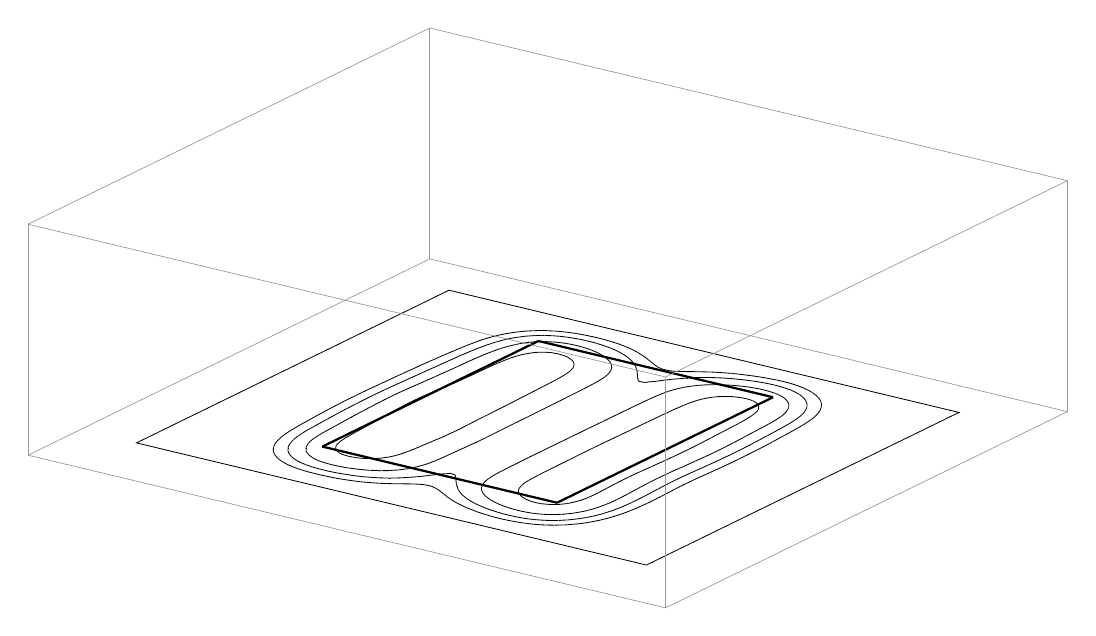
\begin{tikzpicture}
% generated by report/data/gen.py, do not edit
\draw[line width=0.25pt, black!40] (51.03mm,44.32mm) -- (51.03mm,45.05mm);
\draw[line width=0.25pt, black!40] (51.03mm,44.32mm) -- (132.00mm,24.92mm);
\draw[line width=0.25pt, black!40] (51.03mm,44.32mm) -- (0.00mm,19.39mm);
\draw[line width=0.25pt, black!40] (132.00mm,24.92mm) -- (132.00mm,25.65mm);
\draw[line width=0.25pt, black!40] (132.00mm,24.92mm) -- (80.97mm,0.00mm);
\draw[line width=0.25pt, black!40] (0.00mm,19.39mm) -- (0.00mm,20.12mm);
\draw[line width=0.25pt, black!40] (0.00mm,19.39mm) -- (80.97mm,0.00mm);
\draw[line width=0.25pt, black!40] (80.97mm,0.00mm) -- (80.97mm,0.73mm);
\filldraw[fill=white, draw=black, line width=0.30pt] (53.46mm,40.34mm) -- (13.77mm,20.95mm) -- (78.54mm,5.44mm) -- (118.23mm,24.82mm) -- cycle;
\draw[line width=0.30pt] (53.22mm,32.28mm) -- (53.30mm,32.31mm);
\draw[line width=0.30pt] (52.74mm,32.07mm) -- (53.22mm,32.28mm);
\draw[line width=0.30pt] (52.26mm,31.86mm) -- (52.74mm,32.07mm);
\draw[line width=0.30pt] (51.78mm,31.65mm) -- (52.26mm,31.86mm);
\draw[line width=0.30pt] (51.30mm,31.44mm) -- (51.78mm,31.65mm);
\draw[line width=0.30pt] (50.83mm,31.23mm) -- (51.30mm,31.44mm);
\draw[line width=0.30pt] (50.36mm,31.02mm) -- (50.83mm,31.23mm);
\draw[line width=0.30pt] (49.88mm,30.81mm) -- (50.36mm,31.02mm);
\draw[line width=0.30pt] (49.41mm,30.59mm) -- (49.88mm,30.81mm);
\draw[line width=0.30pt] (48.94mm,30.38mm) -- (49.41mm,30.59mm);
\draw[line width=0.30pt] (48.47mm,30.17mm) -- (48.94mm,30.38mm);
\draw[line width=0.30pt] (48.00mm,29.96mm) -- (48.47mm,30.17mm);
\draw[line width=0.30pt] (47.54mm,29.74mm) -- (48.00mm,29.96mm);
\draw[line width=0.30pt] (47.07mm,29.53mm) -- (47.54mm,29.74mm);
\draw[line width=0.30pt] (46.61mm,29.32mm) -- (47.07mm,29.53mm);
\draw[line width=0.30pt] (46.15mm,29.10mm) -- (46.61mm,29.32mm);
\draw[line width=0.30pt] (45.69mm,28.89mm) -- (46.15mm,29.10mm);
\draw[line width=0.30pt] (45.23mm,28.67mm) -- (45.69mm,28.89mm);
\draw[line width=0.30pt] (44.77mm,28.46mm) -- (45.23mm,28.67mm);
\draw[line width=0.30pt] (44.31mm,28.24mm) -- (44.77mm,28.46mm);
\draw[line width=0.30pt] (43.85mm,28.03mm) -- (44.31mm,28.24mm);
\draw[line width=0.30pt] (43.39mm,27.82mm) -- (43.85mm,28.03mm);
\draw[line width=0.30pt] (42.93mm,27.60mm) -- (43.39mm,27.82mm);
\draw[line width=0.30pt] (42.48mm,27.38mm) -- (42.93mm,27.60mm);
\draw[line width=0.30pt] (42.03mm,27.17mm) -- (42.48mm,27.38mm);
\draw[line width=0.30pt] (41.58mm,26.95mm) -- (42.03mm,27.17mm);
\draw[line width=0.30pt] (41.13mm,26.73mm) -- (41.58mm,26.95mm);
\draw[line width=0.30pt] (40.69mm,26.51mm) -- (41.13mm,26.73mm);
\draw[line width=0.30pt] (40.25mm,26.30mm) -- (40.69mm,26.51mm);
\draw[line width=0.30pt] (39.81mm,26.07mm) -- (40.25mm,26.30mm);
\draw[line width=0.30pt] (39.38mm,25.85mm) -- (39.81mm,26.07mm);
\draw[line width=0.30pt] (38.96mm,25.63mm) -- (39.38mm,25.85mm);
\draw[line width=0.30pt] (38.53mm,25.41mm) -- (38.96mm,25.63mm);
\draw[line width=0.30pt] (38.11mm,25.18mm) -- (38.53mm,25.41mm);
\draw[line width=0.30pt] (37.70mm,24.96mm) -- (38.11mm,25.18mm);
\draw[line width=0.30pt] (37.28mm,24.73mm) -- (37.70mm,24.96mm);
\draw[line width=0.30pt] (36.86mm,24.51mm) -- (37.28mm,24.73mm);
\draw[line width=0.30pt] (36.45mm,24.28mm) -- (36.86mm,24.51mm);
\draw[line width=0.30pt] (36.04mm,24.06mm) -- (36.45mm,24.28mm);
\draw[line width=0.30pt] (35.63mm,23.83mm) -- (36.04mm,24.06mm);
\draw[line width=0.30pt] (35.22mm,23.60mm) -- (35.63mm,23.83mm);
\draw[line width=0.30pt] (34.81mm,23.38mm) -- (35.22mm,23.60mm);
\draw[line width=0.30pt] (34.41mm,23.15mm) -- (34.81mm,23.38mm);
\draw[line width=0.30pt] (34.01mm,22.92mm) -- (34.41mm,23.15mm);
\draw[line width=0.30pt] (33.74mm,22.76mm) -- (34.01mm,22.92mm);
\draw[line width=0.30pt] (57.83mm,34.10mm) -- (58.39mm,34.27mm);
\draw[line width=0.30pt] (57.26mm,33.91mm) -- (57.83mm,34.10mm);
\draw[line width=0.30pt] (56.72mm,33.71mm) -- (57.26mm,33.91mm);
\draw[line width=0.30pt] (56.20mm,33.51mm) -- (56.72mm,33.71mm);
\draw[line width=0.30pt] (55.68mm,33.31mm) -- (56.20mm,33.51mm);
\draw[line width=0.30pt] (55.18mm,33.11mm) -- (55.68mm,33.31mm);
\draw[line width=0.30pt] (54.68mm,32.90mm) -- (55.18mm,33.11mm);
\draw[line width=0.30pt] (54.19mm,32.69mm) -- (54.68mm,32.90mm);
\draw[line width=0.30pt] (53.70mm,32.49mm) -- (54.19mm,32.69mm);
\draw[line width=0.30pt] (53.30mm,32.31mm) -- (53.70mm,32.49mm);
\draw[line width=0.30pt] (33.74mm,22.76mm) -- (33.62mm,22.69mm);
\draw[line width=0.30pt] (33.24mm,22.45mm) -- (33.62mm,22.69mm);
\draw[line width=0.30pt] (32.88mm,22.22mm) -- (33.24mm,22.45mm);
\draw[line width=0.30pt] (32.53mm,21.97mm) -- (32.88mm,22.22mm);
\draw[line width=0.30pt] (32.21mm,21.73mm) -- (32.53mm,21.97mm);
\draw[line width=0.30pt] (31.92mm,21.47mm) -- (32.21mm,21.73mm);
\draw[line width=0.30pt] (31.66mm,21.21mm) -- (31.92mm,21.47mm);
\draw[line width=0.30pt] (60.43mm,34.77mm) -- (60.55mm,34.79mm);
\draw[line width=0.30pt] (59.72mm,34.62mm) -- (60.43mm,34.77mm);
\draw[line width=0.30pt] (59.05mm,34.45mm) -- (59.72mm,34.62mm);
\draw[line width=0.30pt] (58.42mm,34.28mm) -- (59.05mm,34.45mm);
\draw[line width=0.30pt] (58.39mm,34.27mm) -- (58.42mm,34.28mm);
\draw[line width=0.30pt] (31.66mm,21.21mm) -- (31.66mm,21.21mm);
\draw[line width=0.30pt] (31.44mm,20.94mm) -- (31.66mm,21.21mm);
\draw[line width=0.30pt] (31.28mm,20.65mm) -- (31.44mm,20.94mm);
\draw[line width=0.30pt] (31.20mm,20.46mm) -- (31.28mm,20.65mm);
\draw[line width=0.30pt] (62.06mm,35.03mm) -- (62.13mm,35.04mm);
\draw[line width=0.30pt] (61.21mm,34.91mm) -- (62.06mm,35.03mm);
\draw[line width=0.30pt] (60.55mm,34.79mm) -- (61.21mm,34.91mm);
\draw[line width=0.30pt] (31.20mm,20.46mm) -- (31.17mm,20.35mm);
\draw[line width=0.30pt] (31.15mm,20.04mm) -- (31.17mm,20.35mm);
\draw[line width=0.30pt] (31.16mm,19.91mm) -- (31.15mm,20.04mm);
\draw[line width=0.30pt] (63.01mm,35.13mm) -- (63.47mm,35.16mm);
\draw[line width=0.30pt] (62.13mm,35.04mm) -- (63.01mm,35.13mm);
\draw[line width=0.30pt] (31.16mm,19.91mm) -- (31.22mm,19.69mm);
\draw[line width=0.30pt] (31.33mm,19.46mm) -- (31.22mm,19.69mm);
\draw[line width=0.30pt] (64.09mm,35.19mm) -- (64.65mm,35.21mm);
\draw[line width=0.30pt] (63.47mm,35.16mm) -- (64.09mm,35.19mm);
\draw[line width=0.30pt] (31.33mm,19.46mm) -- (31.44mm,19.32mm);
\draw[line width=0.30pt] (31.64mm,19.08mm) -- (31.44mm,19.32mm);
\draw[line width=0.30pt] (65.37mm,35.21mm) -- (65.73mm,35.21mm);
\draw[line width=0.30pt] (64.65mm,35.21mm) -- (65.37mm,35.21mm);
\draw[line width=0.30pt] (31.64mm,19.08mm) -- (31.85mm,18.89mm);
\draw[line width=0.30pt] (32.04mm,18.75mm) -- (31.85mm,18.89mm);
\draw[line width=0.30pt] (65.73mm,35.21mm) -- (66.73mm,35.16mm);
\draw[line width=0.30pt] (32.04mm,18.75mm) -- (32.50mm,18.45mm);
\draw[line width=0.30pt] (67.00mm,35.15mm) -- (67.66mm,35.09mm);
\draw[line width=0.30pt] (66.73mm,35.16mm) -- (67.00mm,35.15mm);
\draw[line width=0.30pt] (32.50mm,18.45mm) -- (32.62mm,18.38mm);
\draw[line width=0.30pt] (33.03mm,18.17mm) -- (32.62mm,18.38mm);
\draw[line width=0.30pt] (67.66mm,35.09mm) -- (68.55mm,34.99mm);
\draw[line width=0.30pt] (33.03mm,18.17mm) -- (33.60mm,17.93mm);
\draw[line width=0.30pt] (68.55mm,34.99mm) -- (69.40mm,34.88mm);
\draw[line width=0.30pt] (33.60mm,17.93mm) -- (34.22mm,17.69mm);
\draw[line width=0.30pt] (69.63mm,34.84mm) -- (70.21mm,34.74mm);
\draw[line width=0.30pt] (69.40mm,34.88mm) -- (69.63mm,34.84mm);
\draw[line width=0.30pt] (34.22mm,17.69mm) -- (34.41mm,17.63mm);
\draw[line width=0.30pt] (34.87mm,17.48mm) -- (34.41mm,17.63mm);
\draw[line width=0.30pt] (70.21mm,34.74mm) -- (70.98mm,34.59mm);
\draw[line width=0.30pt] (34.87mm,17.48mm) -- (35.55mm,17.28mm);
\draw[line width=0.30pt] (70.98mm,34.59mm) -- (71.74mm,34.43mm);
\draw[line width=0.30pt] (35.55mm,17.28mm) -- (36.25mm,17.10mm);
\draw[line width=0.30pt] (71.74mm,34.43mm) -- (72.47mm,34.26mm);
\draw[line width=0.30pt] (36.25mm,17.10mm) -- (36.97mm,16.92mm);
\draw[line width=0.30pt] (72.47mm,34.26mm) -- (73.18mm,34.08mm);
\draw[line width=0.30pt] (36.97mm,16.92mm) -- (37.72mm,16.76mm);
\draw[line width=0.30pt] (73.18mm,34.08mm) -- (73.86mm,33.88mm);
\draw[line width=0.30pt] (37.72mm,16.76mm) -- (38.48mm,16.60mm);
\draw[line width=0.30pt] (73.86mm,33.88mm) -- (74.53mm,33.68mm);
\draw[line width=0.30pt] (38.48mm,16.60mm) -- (39.26mm,16.45mm);
\draw[line width=0.30pt] (74.53mm,33.68mm) -- (74.62mm,33.65mm);
\draw[line width=0.30pt] (75.16mm,33.46mm) -- (74.62mm,33.65mm);
\draw[line width=0.30pt] (39.56mm,16.40mm) -- (40.06mm,16.31mm);
\draw[line width=0.30pt] (39.26mm,16.45mm) -- (39.56mm,16.40mm);
\draw[line width=0.30pt] (75.16mm,33.46mm) -- (75.77mm,33.22mm);
\draw[line width=0.30pt] (40.06mm,16.31mm) -- (40.89mm,16.19mm);
\draw[line width=0.30pt] (75.77mm,33.22mm) -- (76.36mm,32.98mm);
\draw[line width=0.30pt] (40.89mm,16.19mm) -- (41.75mm,16.07mm);
\draw[line width=0.30pt] (76.36mm,32.98mm) -- (76.69mm,32.82mm);
\draw[line width=0.30pt] (76.91mm,32.72mm) -- (76.69mm,32.82mm);
\draw[line width=0.30pt] (41.75mm,16.07mm) -- (42.63mm,15.97mm);
\draw[line width=0.30pt] (76.91mm,32.72mm) -- (77.42mm,32.44mm);
\draw[line width=0.30pt] (42.71mm,15.97mm) -- (43.55mm,15.90mm);
\draw[line width=0.30pt] (42.63mm,15.97mm) -- (42.71mm,15.97mm);
\draw[line width=0.30pt] (77.42mm,32.44mm) -- (77.76mm,32.24mm);
\draw[line width=0.30pt] (77.91mm,32.15mm) -- (77.76mm,32.24mm);
\draw[line width=0.30pt] (43.55mm,15.90mm) -- (44.51mm,15.83mm);
\draw[line width=0.30pt] (77.91mm,32.15mm) -- (78.36mm,31.84mm);
\draw[line width=0.30pt] (44.66mm,15.82mm) -- (45.51mm,15.79mm);
\draw[line width=0.30pt] (44.51mm,15.83mm) -- (44.66mm,15.82mm);
\draw[line width=0.30pt] (78.36mm,31.84mm) -- (78.49mm,31.75mm);
\draw[line width=0.30pt] (78.78mm,31.51mm) -- (78.49mm,31.75mm);
\draw[line width=0.30pt] (46.25mm,15.77mm) -- (46.54mm,15.76mm);
\draw[line width=0.30pt] (45.51mm,15.79mm) -- (46.25mm,15.77mm);
\draw[line width=0.30pt] (78.78mm,31.51mm) -- (79.06mm,31.28mm);
\draw[line width=0.30pt] (79.18mm,31.18mm) -- (79.06mm,31.28mm);
\draw[line width=0.30pt] (46.54mm,15.76mm) -- (47.59mm,15.75mm);
\draw[line width=0.30pt] (79.18mm,31.18mm) -- (79.59mm,30.85mm);
\draw[line width=0.30pt] (47.69mm,15.75mm) -- (48.66mm,15.74mm);
\draw[line width=0.30pt] (47.59mm,15.75mm) -- (47.69mm,15.75mm);
\draw[line width=0.30pt] (79.59mm,30.85mm) -- (79.64mm,30.82mm);
\draw[line width=0.30pt] (80.04mm,30.54mm) -- (79.64mm,30.82mm);
\draw[line width=0.30pt] (49.18mm,15.72mm) -- (49.66mm,15.70mm);
\draw[line width=0.30pt] (48.66mm,15.74mm) -- (49.18mm,15.72mm);
\draw[line width=0.30pt] (80.04mm,30.54mm) -- (80.63mm,30.30mm);
\draw[line width=0.30pt] (49.66mm,15.70mm) -- (50.55mm,15.61mm);
\draw[line width=0.30pt] (80.63mm,30.30mm) -- (81.37mm,30.13mm);
\draw[line width=0.30pt] (50.55mm,15.61mm) -- (51.28mm,15.43mm);
\draw[line width=0.30pt] (81.37mm,30.13mm) -- (82.27mm,30.04mm);
\draw[line width=0.30pt] (51.28mm,15.43mm) -- (51.84mm,15.17mm);
\draw[line width=0.30pt] (82.97mm,30.02mm) -- (83.29mm,30.01mm);
\draw[line width=0.30pt] (82.27mm,30.04mm) -- (82.97mm,30.02mm);
\draw[line width=0.30pt] (51.84mm,15.17mm) -- (52.02mm,15.04mm);
\draw[line width=0.30pt] (52.29mm,14.87mm) -- (52.02mm,15.04mm);
\draw[line width=0.30pt] (83.29mm,30.01mm) -- (84.35mm,30.00mm);
\draw[line width=0.30pt] (52.29mm,14.87mm) -- (52.66mm,14.56mm);
\draw[line width=0.30pt] (52.70mm,14.53mm) -- (52.66mm,14.56mm);
\draw[line width=0.30pt] (84.43mm,30.00mm) -- (85.40mm,29.98mm);
\draw[line width=0.30pt] (84.35mm,30.00mm) -- (84.43mm,30.00mm);
\draw[line width=0.30pt] (52.70mm,14.53mm) -- (53.11mm,14.21mm);
\draw[line width=0.30pt] (85.89mm,29.97mm) -- (86.44mm,29.96mm);
\draw[line width=0.30pt] (85.40mm,29.98mm) -- (85.89mm,29.97mm);
\draw[line width=0.30pt] (53.11mm,14.21mm) -- (53.25mm,14.09mm);
\draw[line width=0.30pt] (53.54mm,13.89mm) -- (53.25mm,14.09mm);
\draw[line width=0.30pt] (86.44mm,29.96mm) -- (87.44mm,29.92mm);
\draw[line width=0.30pt] (53.54mm,13.89mm) -- (53.99mm,13.59mm);
\draw[line width=0.30pt] (54.00mm,13.58mm) -- (53.99mm,13.59mm);
\draw[line width=0.30pt] (87.50mm,29.91mm) -- (88.40mm,29.85mm);
\draw[line width=0.30pt] (87.44mm,29.92mm) -- (87.50mm,29.91mm);
\draw[line width=0.30pt] (54.00mm,13.58mm) -- (54.51mm,13.30mm);
\draw[line width=0.30pt] (88.40mm,29.85mm) -- (89.33mm,29.78mm);
\draw[line width=0.30pt] (54.51mm,13.30mm) -- (55.03mm,13.03mm);
\draw[line width=0.30pt] (89.46mm,29.77mm) -- (90.23mm,29.69mm);
\draw[line width=0.30pt] (89.33mm,29.78mm) -- (89.46mm,29.77mm);
\draw[line width=0.30pt] (55.03mm,13.03mm) -- (55.08mm,13.01mm);
\draw[line width=0.30pt] (55.59mm,12.77mm) -- (55.08mm,13.01mm);
\draw[line width=0.30pt] (90.23mm,29.69mm) -- (91.10mm,29.58mm);
\draw[line width=0.30pt] (55.59mm,12.77mm) -- (56.18mm,12.53mm);
\draw[line width=0.30pt] (91.10mm,29.58mm) -- (91.96mm,29.47mm);
\draw[line width=0.30pt] (56.18mm,12.53mm) -- (56.79mm,12.29mm);
\draw[line width=0.30pt] (92.17mm,29.44mm) -- (92.79mm,29.35mm);
\draw[line width=0.30pt] (91.96mm,29.47mm) -- (92.17mm,29.44mm);
\draw[line width=0.30pt] (56.79mm,12.29mm) -- (56.98mm,12.22mm);
\draw[line width=0.30pt] (57.42mm,12.07mm) -- (56.98mm,12.22mm);
\draw[line width=0.30pt] (92.79mm,29.35mm) -- (93.60mm,29.22mm);
\draw[line width=0.30pt] (57.42mm,12.07mm) -- (58.07mm,11.86mm);
\draw[line width=0.30pt] (93.60mm,29.22mm) -- (94.39mm,29.07mm);
\draw[line width=0.30pt] (58.07mm,11.86mm) -- (58.75mm,11.66mm);
\draw[line width=0.30pt] (94.39mm,29.07mm) -- (95.16mm,28.92mm);
\draw[line width=0.30pt] (58.75mm,11.66mm) -- (59.44mm,11.47mm);
\draw[line width=0.30pt] (95.16mm,28.92mm) -- (95.90mm,28.75mm);
\draw[line width=0.30pt] (59.44mm,11.47mm) -- (60.16mm,11.29mm);
\draw[line width=0.30pt] (95.90mm,28.75mm) -- (96.61mm,28.57mm);
\draw[line width=0.30pt] (60.16mm,11.29mm) -- (60.91mm,11.13mm);
\draw[line width=0.30pt] (96.61mm,28.57mm) -- (97.28mm,28.37mm);
\draw[line width=0.30pt] (60.91mm,11.13mm) -- (61.68mm,10.98mm);
\draw[line width=0.30pt] (97.28mm,28.37mm) -- (97.92mm,28.15mm);
\draw[line width=0.30pt] (61.68mm,10.98mm) -- (62.49mm,10.84mm);
\draw[line width=0.30pt] (97.92mm,28.15mm) -- (98.46mm,27.94mm);
\draw[line width=0.30pt] (98.52mm,27.91mm) -- (98.46mm,27.94mm);
\draw[line width=0.30pt] (63.19mm,10.74mm) -- (63.33mm,10.72mm);
\draw[line width=0.30pt] (62.49mm,10.84mm) -- (63.19mm,10.74mm);
\draw[line width=0.30pt] (98.52mm,27.91mm) -- (99.07mm,27.65mm);
\draw[line width=0.30pt] (63.33mm,10.72mm) -- (64.21mm,10.62mm);
\draw[line width=0.30pt] (99.07mm,27.65mm) -- (99.58mm,27.37mm);
\draw[line width=0.30pt] (64.21mm,10.62mm) -- (65.15mm,10.55mm);
\draw[line width=0.30pt] (99.58mm,27.37mm) -- (99.63mm,27.33mm);
\draw[line width=0.30pt] (100.01mm,27.05mm) -- (99.63mm,27.33mm);
\draw[line width=0.30pt] (65.38mm,10.54mm) -- (66.15mm,10.51mm);
\draw[line width=0.30pt] (65.15mm,10.55mm) -- (65.38mm,10.54mm);
\draw[line width=0.30pt] (100.01mm,27.05mm) -- (100.22mm,26.86mm);
\draw[line width=0.30pt] (100.38mm,26.70mm) -- (100.22mm,26.86mm);
\draw[line width=0.30pt] (66.88mm,10.50mm) -- (67.23mm,10.51mm);
\draw[line width=0.30pt] (66.15mm,10.51mm) -- (66.88mm,10.50mm);
\draw[line width=0.30pt] (100.38mm,26.70mm) -- (100.56mm,26.46mm);
\draw[line width=0.30pt] (100.65mm,26.30mm) -- (100.56mm,26.46mm);
\draw[line width=0.30pt] (68.11mm,10.53mm) -- (68.40mm,10.55mm);
\draw[line width=0.30pt] (67.23mm,10.51mm) -- (68.11mm,10.53mm);
\draw[line width=0.30pt] (100.65mm,26.30mm) -- (100.72mm,26.10mm);
\draw[line width=0.30pt] (100.77mm,25.83mm) -- (100.72mm,26.10mm);
\draw[line width=0.30pt] (69.16mm,10.61mm) -- (69.71mm,10.66mm);
\draw[line width=0.30pt] (68.40mm,10.55mm) -- (69.16mm,10.61mm);
\draw[line width=0.30pt] (100.77mm,25.83mm) -- (100.77mm,25.76mm);
\draw[line width=0.30pt] (100.73mm,25.44mm) -- (100.77mm,25.76mm);
\draw[line width=0.30pt] (100.66mm,25.25mm) -- (100.73mm,25.44mm);
\draw[line width=0.30pt] (70.97mm,10.82mm) -- (71.21mm,10.86mm);
\draw[line width=0.30pt] (70.11mm,10.70mm) -- (70.97mm,10.82mm);
\draw[line width=0.30pt] (69.71mm,10.66mm) -- (70.11mm,10.70mm);
\draw[line width=0.30pt] (100.66mm,25.25mm) -- (100.62mm,25.15mm);
\draw[line width=0.30pt] (100.45mm,24.86mm) -- (100.62mm,25.15mm);
\draw[line width=0.30pt] (100.23mm,24.59mm) -- (100.45mm,24.86mm);
\draw[line width=0.30pt] (100.08mm,24.43mm) -- (100.23mm,24.59mm);
\draw[line width=0.30pt] (72.49mm,11.11mm) -- (73.08mm,11.24mm);
\draw[line width=0.30pt] (71.75mm,10.96mm) -- (72.49mm,11.11mm);
\draw[line width=0.30pt] (71.21mm,10.86mm) -- (71.75mm,10.96mm);
\draw[line width=0.30pt] (100.08mm,24.43mm) -- (99.97mm,24.33mm);
\draw[line width=0.30pt] (99.67mm,24.07mm) -- (99.97mm,24.33mm);
\draw[line width=0.30pt] (99.35mm,23.83mm) -- (99.67mm,24.07mm);
\draw[line width=0.30pt] (98.99mm,23.59mm) -- (99.35mm,23.83mm);
\draw[line width=0.30pt] (98.62mm,23.35mm) -- (98.99mm,23.59mm);
\draw[line width=0.30pt] (98.24mm,23.12mm) -- (98.62mm,23.35mm);
\draw[line width=0.30pt] (97.84mm,22.89mm) -- (98.24mm,23.12mm);
\draw[line width=0.30pt] (97.44mm,22.66mm) -- (97.84mm,22.89mm);
\draw[line width=0.30pt] (97.03mm,22.44mm) -- (97.44mm,22.66mm);
\draw[line width=0.30pt] (96.69mm,22.25mm) -- (97.03mm,22.44mm);
\draw[line width=0.30pt] (75.57mm,11.99mm) -- (76.08mm,12.18mm);
\draw[line width=0.30pt] (75.01mm,11.80mm) -- (75.57mm,11.99mm);
\draw[line width=0.30pt] (74.43mm,11.62mm) -- (75.01mm,11.80mm);
\draw[line width=0.30pt] (73.82mm,11.44mm) -- (74.43mm,11.62mm);
\draw[line width=0.30pt] (73.18mm,11.27mm) -- (73.82mm,11.44mm);
\draw[line width=0.30pt] (73.08mm,11.24mm) -- (73.18mm,11.27mm);
\draw[line width=0.30pt] (96.69mm,22.25mm) -- (96.62mm,22.21mm);
\draw[line width=0.30pt] (96.21mm,21.98mm) -- (96.62mm,22.21mm);
\draw[line width=0.30pt] (95.80mm,21.76mm) -- (96.21mm,21.98mm);
\draw[line width=0.30pt] (95.38mm,21.53mm) -- (95.80mm,21.76mm);
\draw[line width=0.30pt] (94.97mm,21.31mm) -- (95.38mm,21.53mm);
\draw[line width=0.30pt] (94.55mm,21.08mm) -- (94.97mm,21.31mm);
\draw[line width=0.30pt] (94.14mm,20.86mm) -- (94.55mm,21.08mm);
\draw[line width=0.30pt] (93.71mm,20.63mm) -- (94.14mm,20.86mm);
\draw[line width=0.30pt] (93.29mm,20.41mm) -- (93.71mm,20.63mm);
\draw[line width=0.30pt] (92.86mm,20.19mm) -- (93.29mm,20.41mm);
\draw[line width=0.30pt] (92.43mm,19.97mm) -- (92.86mm,20.19mm);
\draw[line width=0.30pt] (92.00mm,19.75mm) -- (92.43mm,19.97mm);
\draw[line width=0.30pt] (91.56mm,19.53mm) -- (92.00mm,19.75mm);
\draw[line width=0.30pt] (91.11mm,19.31mm) -- (91.56mm,19.53mm);
\draw[line width=0.30pt] (90.67mm,19.09mm) -- (91.11mm,19.31mm);
\draw[line width=0.30pt] (90.22mm,18.87mm) -- (90.67mm,19.09mm);
\draw[line width=0.30pt] (89.77mm,18.65mm) -- (90.22mm,18.87mm);
\draw[line width=0.30pt] (89.32mm,18.44mm) -- (89.77mm,18.65mm);
\draw[line width=0.30pt] (88.87mm,18.22mm) -- (89.32mm,18.44mm);
\draw[line width=0.30pt] (88.41mm,18.01mm) -- (88.87mm,18.22mm);
\draw[line width=0.30pt] (87.95mm,17.79mm) -- (88.41mm,18.01mm);
\draw[line width=0.30pt] (87.48mm,17.58mm) -- (87.95mm,17.79mm);
\draw[line width=0.30pt] (87.01mm,17.37mm) -- (87.48mm,17.58mm);
\draw[line width=0.30pt] (86.54mm,17.16mm) -- (87.01mm,17.37mm);
\draw[line width=0.30pt] (86.07mm,16.94mm) -- (86.54mm,17.16mm);
\draw[line width=0.30pt] (85.60mm,16.73mm) -- (86.07mm,16.94mm);
\draw[line width=0.30pt] (85.13mm,16.52mm) -- (85.60mm,16.73mm);
\draw[line width=0.30pt] (84.67mm,16.31mm) -- (85.13mm,16.52mm);
\draw[line width=0.30pt] (84.21mm,16.09mm) -- (84.67mm,16.31mm);
\draw[line width=0.30pt] (83.76mm,15.87mm) -- (84.21mm,16.09mm);
\draw[line width=0.30pt] (83.31mm,15.66mm) -- (83.76mm,15.87mm);
\draw[line width=0.30pt] (82.87mm,15.44mm) -- (83.31mm,15.66mm);
\draw[line width=0.30pt] (82.44mm,15.22mm) -- (82.87mm,15.44mm);
\draw[line width=0.30pt] (82.01mm,15.00mm) -- (82.44mm,15.22mm);
\draw[line width=0.30pt] (81.58mm,14.77mm) -- (82.01mm,15.00mm);
\draw[line width=0.30pt] (81.16mm,14.55mm) -- (81.58mm,14.77mm);
\draw[line width=0.30pt] (80.73mm,14.33mm) -- (81.16mm,14.55mm);
\draw[line width=0.30pt] (80.30mm,14.11mm) -- (80.73mm,14.33mm);
\draw[line width=0.30pt] (79.87mm,13.88mm) -- (80.30mm,14.11mm);
\draw[line width=0.30pt] (79.43mm,13.67mm) -- (79.87mm,13.88mm);
\draw[line width=0.30pt] (78.99mm,13.45mm) -- (79.43mm,13.67mm);
\draw[line width=0.30pt] (78.53mm,13.23mm) -- (78.99mm,13.45mm);
\draw[line width=0.30pt] (78.07mm,13.02mm) -- (78.53mm,13.23mm);
\draw[line width=0.30pt] (77.60mm,12.81mm) -- (78.07mm,13.02mm);
\draw[line width=0.30pt] (77.11mm,12.60mm) -- (77.60mm,12.81mm);
\draw[line width=0.30pt] (76.62mm,12.39mm) -- (77.11mm,12.60mm);
\draw[line width=0.30pt] (76.10mm,12.19mm) -- (76.62mm,12.39mm);
\draw[line width=0.30pt] (76.08mm,12.18mm) -- (76.10mm,12.19mm);
\draw[line width=0.30pt] (54.66mm,31.93mm) -- (54.90mm,32.04mm);
\draw[line width=0.30pt] (54.19mm,31.72mm) -- (54.66mm,31.93mm);
\draw[line width=0.30pt] (53.72mm,31.51mm) -- (54.19mm,31.72mm);
\draw[line width=0.30pt] (53.25mm,31.30mm) -- (53.72mm,31.51mm);
\draw[line width=0.30pt] (52.78mm,31.09mm) -- (53.25mm,31.30mm);
\draw[line width=0.30pt] (52.31mm,30.87mm) -- (52.78mm,31.09mm);
\draw[line width=0.30pt] (51.84mm,30.66mm) -- (52.31mm,30.87mm);
\draw[line width=0.30pt] (51.37mm,30.45mm) -- (51.84mm,30.66mm);
\draw[line width=0.30pt] (50.90mm,30.24mm) -- (51.37mm,30.45mm);
\draw[line width=0.30pt] (50.43mm,30.03mm) -- (50.90mm,30.24mm);
\draw[line width=0.30pt] (49.96mm,29.81mm) -- (50.43mm,30.03mm);
\draw[line width=0.30pt] (49.48mm,29.60mm) -- (49.96mm,29.81mm);
\draw[line width=0.30pt] (49.01mm,29.39mm) -- (49.48mm,29.60mm);
\draw[line width=0.30pt] (48.54mm,29.18mm) -- (49.01mm,29.39mm);
\draw[line width=0.30pt] (48.08mm,28.97mm) -- (48.54mm,29.18mm);
\draw[line width=0.30pt] (47.61mm,28.75mm) -- (48.08mm,28.97mm);
\draw[line width=0.30pt] (47.14mm,28.54mm) -- (47.61mm,28.75mm);
\draw[line width=0.30pt] (46.67mm,28.33mm) -- (47.14mm,28.54mm);
\draw[line width=0.30pt] (46.20mm,28.12mm) -- (46.67mm,28.33mm);
\draw[line width=0.30pt] (45.74mm,27.90mm) -- (46.20mm,28.12mm);
\draw[line width=0.30pt] (45.28mm,27.69mm) -- (45.74mm,27.90mm);
\draw[line width=0.30pt] (44.82mm,27.47mm) -- (45.28mm,27.69mm);
\draw[line width=0.30pt] (44.37mm,27.26mm) -- (44.82mm,27.47mm);
\draw[line width=0.30pt] (43.92mm,27.04mm) -- (44.37mm,27.26mm);
\draw[line width=0.30pt] (43.47mm,26.82mm) -- (43.92mm,27.04mm);
\draw[line width=0.30pt] (43.03mm,26.60mm) -- (43.47mm,26.82mm);
\draw[line width=0.30pt] (42.59mm,26.38mm) -- (43.03mm,26.60mm);
\draw[line width=0.30pt] (42.15mm,26.16mm) -- (42.59mm,26.38mm);
\draw[line width=0.30pt] (41.72mm,25.94mm) -- (42.15mm,26.16mm);
\draw[line width=0.30pt] (41.29mm,25.72mm) -- (41.72mm,25.94mm);
\draw[line width=0.30pt] (40.86mm,25.50mm) -- (41.29mm,25.72mm);
\draw[line width=0.30pt] (40.43mm,25.28mm) -- (40.86mm,25.50mm);
\draw[line width=0.30pt] (40.01mm,25.05mm) -- (40.43mm,25.28mm);
\draw[line width=0.30pt] (39.59mm,24.83mm) -- (40.01mm,25.05mm);
\draw[line width=0.30pt] (39.17mm,24.61mm) -- (39.59mm,24.83mm);
\draw[line width=0.30pt] (38.76mm,24.38mm) -- (39.17mm,24.61mm);
\draw[line width=0.30pt] (38.34mm,24.15mm) -- (38.76mm,24.38mm);
\draw[line width=0.30pt] (37.93mm,23.93mm) -- (38.34mm,24.15mm);
\draw[line width=0.30pt] (37.52mm,23.70mm) -- (37.93mm,23.93mm);
\draw[line width=0.30pt] (37.11mm,23.48mm) -- (37.52mm,23.70mm);
\draw[line width=0.30pt] (36.69mm,23.25mm) -- (37.11mm,23.48mm);
\draw[line width=0.30pt] (36.28mm,23.02mm) -- (36.69mm,23.25mm);
\draw[line width=0.30pt] (35.88mm,22.80mm) -- (36.28mm,23.02mm);
\draw[line width=0.30pt] (35.47mm,22.57mm) -- (35.88mm,22.80mm);
\draw[line width=0.30pt] (35.25mm,22.44mm) -- (35.47mm,22.57mm);
\draw[line width=0.30pt] (59.34mm,33.73mm) -- (59.65mm,33.83mm);
\draw[line width=0.30pt] (58.75mm,33.55mm) -- (59.34mm,33.73mm);
\draw[line width=0.30pt] (58.20mm,33.36mm) -- (58.75mm,33.55mm);
\draw[line width=0.30pt] (57.66mm,33.16mm) -- (58.20mm,33.36mm);
\draw[line width=0.30pt] (57.13mm,32.96mm) -- (57.66mm,33.16mm);
\draw[line width=0.30pt] (56.62mm,32.76mm) -- (57.13mm,32.96mm);
\draw[line width=0.30pt] (56.12mm,32.56mm) -- (56.62mm,32.76mm);
\draw[line width=0.30pt] (55.63mm,32.35mm) -- (56.12mm,32.56mm);
\draw[line width=0.30pt] (55.14mm,32.14mm) -- (55.63mm,32.35mm);
\draw[line width=0.30pt] (54.90mm,32.04mm) -- (55.14mm,32.14mm);
\draw[line width=0.30pt] (35.25mm,22.44mm) -- (35.08mm,22.34mm);
\draw[line width=0.30pt] (34.71mm,22.10mm) -- (35.08mm,22.34mm);
\draw[line width=0.30pt] (34.36mm,21.86mm) -- (34.71mm,22.10mm);
\draw[line width=0.30pt] (34.03mm,21.62mm) -- (34.36mm,21.86mm);
\draw[line width=0.30pt] (33.72mm,21.37mm) -- (34.03mm,21.62mm);
\draw[line width=0.30pt] (33.46mm,21.10mm) -- (33.72mm,21.37mm);
\draw[line width=0.30pt] (33.36mm,20.98mm) -- (33.46mm,21.10mm);
\draw[line width=0.30pt] (61.34mm,34.23mm) -- (61.69mm,34.29mm);
\draw[line width=0.30pt] (60.63mm,34.08mm) -- (61.34mm,34.23mm);
\draw[line width=0.30pt] (59.96mm,33.91mm) -- (60.63mm,34.08mm);
\draw[line width=0.30pt] (59.65mm,33.83mm) -- (59.96mm,33.91mm);
\draw[line width=0.30pt] (33.36mm,20.98mm) -- (33.25mm,20.83mm);
\draw[line width=0.30pt] (33.09mm,20.54mm) -- (33.25mm,20.83mm);
\draw[line width=0.30pt] (33.01mm,20.29mm) -- (33.09mm,20.54mm);
\draw[line width=0.30pt] (63.00mm,34.48mm) -- (63.20mm,34.50mm);
\draw[line width=0.30pt] (62.13mm,34.36mm) -- (63.00mm,34.48mm);
\draw[line width=0.30pt] (61.69mm,34.29mm) -- (62.13mm,34.36mm);
\draw[line width=0.30pt] (33.01mm,20.29mm) -- (33.01mm,20.24mm);
\draw[line width=0.30pt] (33.03mm,19.91mm) -- (33.01mm,20.24mm);
\draw[line width=0.30pt] (33.06mm,19.78mm) -- (33.03mm,19.91mm);
\draw[line width=0.30pt] (64.01mm,34.56mm) -- (64.46mm,34.58mm);
\draw[line width=0.30pt] (63.20mm,34.50mm) -- (64.01mm,34.56mm);
\draw[line width=0.30pt] (33.06mm,19.78mm) -- (33.18mm,19.55mm);
\draw[line width=0.30pt] (33.31mm,19.37mm) -- (33.18mm,19.55mm);
\draw[line width=0.30pt] (65.22mm,34.60mm) -- (65.57mm,34.60mm);
\draw[line width=0.30pt] (64.46mm,34.58mm) -- (65.22mm,34.60mm);
\draw[line width=0.30pt] (33.31mm,19.37mm) -- (33.53mm,19.14mm);
\draw[line width=0.30pt] (33.67mm,19.02mm) -- (33.53mm,19.14mm);
\draw[line width=0.30pt] (65.57mm,34.60mm) -- (66.58mm,34.56mm);
\draw[line width=0.30pt] (33.67mm,19.02mm) -- (34.13mm,18.71mm);
\draw[line width=0.30pt] (66.78mm,34.55mm) -- (67.51mm,34.49mm);
\draw[line width=0.30pt] (66.58mm,34.56mm) -- (66.78mm,34.55mm);
\draw[line width=0.30pt] (34.13mm,18.71mm) -- (34.26mm,18.64mm);
\draw[line width=0.30pt] (34.66mm,18.44mm) -- (34.26mm,18.64mm);
\draw[line width=0.30pt] (67.51mm,34.49mm) -- (68.39mm,34.39mm);
\draw[line width=0.30pt] (34.66mm,18.44mm) -- (35.24mm,18.20mm);
\draw[line width=0.30pt] (68.39mm,34.39mm) -- (69.22mm,34.26mm);
\draw[line width=0.30pt] (35.24mm,18.20mm) -- (35.87mm,17.97mm);
\draw[line width=0.30pt] (69.62mm,34.19mm) -- (70.02mm,34.12mm);
\draw[line width=0.30pt] (69.22mm,34.26mm) -- (69.62mm,34.19mm);
\draw[line width=0.30pt] (35.87mm,17.97mm) -- (36.47mm,17.79mm);
\draw[line width=0.30pt] (36.53mm,17.77mm) -- (36.47mm,17.79mm);
\draw[line width=0.30pt] (70.02mm,34.12mm) -- (70.77mm,33.96mm);
\draw[line width=0.30pt] (36.53mm,17.77mm) -- (37.24mm,17.58mm);
\draw[line width=0.30pt] (70.77mm,33.96mm) -- (71.50mm,33.79mm);
\draw[line width=0.30pt] (37.24mm,17.58mm) -- (37.96mm,17.41mm);
\draw[line width=0.30pt] (71.50mm,33.79mm) -- (72.20mm,33.60mm);
\draw[line width=0.30pt] (37.96mm,17.41mm) -- (38.72mm,17.24mm);
\draw[line width=0.30pt] (72.20mm,33.60mm) -- (72.54mm,33.49mm);
\draw[line width=0.30pt] (72.87mm,33.39mm) -- (72.54mm,33.49mm);
\draw[line width=0.30pt] (38.82mm,17.22mm) -- (39.50mm,17.09mm);
\draw[line width=0.30pt] (38.72mm,17.24mm) -- (38.82mm,17.22mm);
\draw[line width=0.30pt] (72.87mm,33.39mm) -- (73.50mm,33.17mm);
\draw[line width=0.30pt] (39.50mm,17.09mm) -- (40.30mm,16.96mm);
\draw[line width=0.30pt] (73.50mm,33.17mm) -- (74.11mm,32.94mm);
\draw[line width=0.30pt] (40.30mm,16.96mm) -- (41.13mm,16.83mm);
\draw[line width=0.30pt] (74.11mm,32.94mm) -- (74.68mm,32.69mm);
\draw[line width=0.30pt] (41.13mm,16.83mm) -- (41.99mm,16.72mm);
\draw[line width=0.30pt] (74.68mm,32.69mm) -- (74.83mm,32.62mm);
\draw[line width=0.30pt] (75.21mm,32.42mm) -- (74.83mm,32.62mm);
\draw[line width=0.30pt] (42.51mm,16.66mm) -- (42.88mm,16.63mm);
\draw[line width=0.30pt] (41.99mm,16.72mm) -- (42.51mm,16.66mm);
\draw[line width=0.30pt] (75.21mm,32.42mm) -- (75.71mm,32.13mm);
\draw[line width=0.30pt] (42.88mm,16.63mm) -- (43.82mm,16.56mm);
\draw[line width=0.30pt] (75.71mm,32.13mm) -- (75.82mm,32.06mm);
\draw[line width=0.30pt] (76.15mm,31.82mm) -- (75.82mm,32.06mm);
\draw[line width=0.30pt] (44.48mm,16.52mm) -- (44.80mm,16.51mm);
\draw[line width=0.30pt] (43.82mm,16.56mm) -- (44.48mm,16.52mm);
\draw[line width=0.30pt] (76.15mm,31.82mm) -- (76.43mm,31.59mm);
\draw[line width=0.30pt] (76.54mm,31.48mm) -- (76.43mm,31.59mm);
\draw[line width=0.30pt] (44.80mm,16.51mm) -- (45.84mm,16.48mm);
\draw[line width=0.30pt] (76.54mm,31.48mm) -- (76.84mm,31.17mm);
\draw[line width=0.30pt] (76.88mm,31.11mm) -- (76.84mm,31.17mm);
\draw[line width=0.30pt] (45.97mm,16.48mm) -- (46.96mm,16.50mm);
\draw[line width=0.30pt] (45.84mm,16.48mm) -- (45.97mm,16.48mm);
\draw[line width=0.30pt] (76.88mm,31.11mm) -- (77.10mm,30.78mm);
\draw[line width=0.30pt] (77.13mm,30.71mm) -- (77.10mm,30.78mm);
\draw[line width=0.30pt] (47.23mm,16.51mm) -- (48.16mm,16.56mm);
\draw[line width=0.30pt] (46.96mm,16.50mm) -- (47.23mm,16.51mm);
\draw[line width=0.30pt] (77.13mm,30.71mm) -- (77.26mm,30.42mm);
\draw[line width=0.30pt] (77.29mm,30.26mm) -- (77.26mm,30.42mm);
\draw[line width=0.30pt] (49.35mm,16.65mm) -- (49.46mm,16.66mm);
\draw[line width=0.30pt] (48.34mm,16.57mm) -- (49.35mm,16.65mm);
\draw[line width=0.30pt] (48.16mm,16.56mm) -- (48.34mm,16.57mm);
\draw[line width=0.30pt] (77.29mm,30.26mm) -- (77.35mm,30.07mm);
\draw[line width=0.30pt] (77.37mm,29.76mm) -- (77.35mm,30.07mm);
\draw[line width=0.30pt] (50.31mm,16.74mm) -- (50.86mm,16.82mm);
\draw[line width=0.30pt] (49.46mm,16.66mm) -- (50.31mm,16.74mm);
\draw[line width=0.30pt] (77.37mm,29.76mm) -- (77.38mm,29.74mm);
\draw[line width=0.30pt] (77.41mm,29.41mm) -- (77.38mm,29.74mm);
\draw[line width=0.30pt] (77.36mm,29.23mm) -- (77.41mm,29.41mm);
\draw[line width=0.30pt] (52.11mm,16.96mm) -- (52.31mm,16.99mm);
\draw[line width=0.30pt] (51.23mm,16.85mm) -- (52.11mm,16.96mm);
\draw[line width=0.30pt] (50.86mm,16.82mm) -- (51.23mm,16.85mm);
\draw[line width=0.30pt] (77.36mm,29.23mm) -- (77.47mm,29.07mm);
\draw[line width=0.30pt] (77.52mm,28.78mm) -- (77.47mm,29.07mm);
\draw[line width=0.30pt] (53.13mm,17.04mm) -- (53.59mm,17.09mm);
\draw[line width=0.30pt] (52.31mm,16.99mm) -- (53.13mm,17.04mm);
\draw[line width=0.30pt] (77.52mm,28.78mm) -- (78.29mm,28.62mm);
\draw[line width=0.30pt] (53.59mm,17.09mm) -- (54.25mm,16.88mm);
\draw[line width=0.30pt] (78.97mm,28.71mm) -- (79.64mm,28.76mm);
\draw[line width=0.30pt] (78.29mm,28.62mm) -- (78.97mm,28.71mm);
\draw[line width=0.30pt] (54.25mm,16.88mm) -- (54.24mm,16.78mm);
\draw[line width=0.30pt] (54.35mm,16.43mm) -- (54.24mm,16.78mm);
\draw[line width=0.30pt] (54.36mm,16.41mm) -- (54.35mm,16.43mm);
\draw[line width=0.30pt] (80.82mm,28.92mm) -- (81.10mm,28.94mm);
\draw[line width=0.30pt] (79.93mm,28.80mm) -- (80.82mm,28.92mm);
\draw[line width=0.30pt] (79.64mm,28.76mm) -- (79.93mm,28.80mm);
\draw[line width=0.30pt] (54.36mm,16.41mm) -- (54.34mm,16.10mm);
\draw[line width=0.30pt] (54.40mm,15.90mm) -- (54.34mm,16.10mm);
\draw[line width=0.30pt] (81.74mm,29.02mm) -- (82.49mm,29.09mm);
\draw[line width=0.30pt] (81.10mm,28.94mm) -- (81.74mm,29.02mm);
\draw[line width=0.30pt] (54.40mm,15.90mm) -- (54.39mm,15.77mm);
\draw[line width=0.30pt] (54.48mm,15.42mm) -- (54.39mm,15.77mm);
\draw[line width=0.30pt] (54.48mm,15.41mm) -- (54.48mm,15.42mm);
\draw[line width=0.30pt] (83.75mm,29.19mm) -- (83.78mm,29.19mm);
\draw[line width=0.30pt] (82.71mm,29.11mm) -- (83.75mm,29.19mm);
\draw[line width=0.30pt] (82.49mm,29.09mm) -- (82.71mm,29.11mm);
\draw[line width=0.30pt] (54.48mm,15.41mm) -- (54.62mm,15.06mm);
\draw[line width=0.30pt] (54.68mm,14.97mm) -- (54.62mm,15.06mm);
\draw[line width=0.30pt] (84.88mm,29.24mm) -- (84.98mm,29.24mm);
\draw[line width=0.30pt] (83.78mm,29.19mm) -- (84.88mm,29.24mm);
\draw[line width=0.30pt] (54.68mm,14.97mm) -- (54.86mm,14.68mm);
\draw[line width=0.30pt] (54.95mm,14.58mm) -- (54.86mm,14.68mm);
\draw[line width=0.30pt] (84.98mm,29.24mm) -- (86.10mm,29.26mm);
\draw[line width=0.30pt] (54.95mm,14.58mm) -- (55.24mm,14.26mm);
\draw[line width=0.30pt] (55.30mm,14.22mm) -- (55.24mm,14.26mm);
\draw[line width=0.30pt] (86.16mm,29.26mm) -- (87.14mm,29.24mm);
\draw[line width=0.30pt] (86.10mm,29.26mm) -- (86.16mm,29.26mm);
\draw[line width=0.30pt] (55.30mm,14.22mm) -- (55.71mm,13.89mm);
\draw[line width=0.30pt] (87.66mm,29.22mm) -- (88.14mm,29.20mm);
\draw[line width=0.30pt] (87.14mm,29.24mm) -- (87.66mm,29.22mm);
\draw[line width=0.30pt] (55.71mm,13.89mm) -- (55.84mm,13.80mm);
\draw[line width=0.30pt] (56.18mm,13.59mm) -- (55.84mm,13.80mm);
\draw[line width=0.30pt] (88.14mm,29.20mm) -- (89.10mm,29.13mm);
\draw[line width=0.30pt] (56.18mm,13.59mm) -- (56.68mm,13.30mm);
\draw[line width=0.30pt] (89.54mm,29.10mm) -- (90.01mm,29.05mm);
\draw[line width=0.30pt] (89.10mm,29.13mm) -- (89.54mm,29.10mm);
\draw[line width=0.30pt] (56.68mm,13.30mm) -- (56.80mm,13.24mm);
\draw[line width=0.30pt] (57.23mm,13.04mm) -- (56.80mm,13.24mm);
\draw[line width=0.30pt] (90.01mm,29.05mm) -- (90.90mm,28.96mm);
\draw[line width=0.30pt] (57.23mm,13.04mm) -- (57.81mm,12.79mm);
\draw[line width=0.30pt] (90.90mm,28.96mm) -- (91.76mm,28.85mm);
\draw[line width=0.30pt] (57.81mm,12.79mm) -- (58.41mm,12.56mm);
\draw[line width=0.30pt] (92.20mm,28.79mm) -- (92.60mm,28.73mm);
\draw[line width=0.30pt] (91.76mm,28.85mm) -- (92.20mm,28.79mm);
\draw[line width=0.30pt] (58.41mm,12.56mm) -- (58.64mm,12.48mm);
\draw[line width=0.30pt] (59.05mm,12.34mm) -- (58.64mm,12.48mm);
\draw[line width=0.30pt] (92.60mm,28.73mm) -- (93.40mm,28.59mm);
\draw[line width=0.30pt] (59.05mm,12.34mm) -- (59.71mm,12.13mm);
\draw[line width=0.30pt] (93.40mm,28.59mm) -- (94.17mm,28.44mm);
\draw[line width=0.30pt] (59.71mm,12.13mm) -- (60.39mm,11.94mm);
\draw[line width=0.30pt] (94.17mm,28.44mm) -- (94.91mm,28.27mm);
\draw[line width=0.30pt] (60.39mm,11.94mm) -- (61.11mm,11.76mm);
\draw[line width=0.30pt] (94.91mm,28.27mm) -- (95.61mm,28.08mm);
\draw[line width=0.30pt] (61.11mm,11.76mm) -- (61.85mm,11.59mm);
\draw[line width=0.30pt] (95.61mm,28.08mm) -- (96.28mm,27.87mm);
\draw[line width=0.30pt] (61.85mm,11.59mm) -- (62.64mm,11.44mm);
\draw[line width=0.30pt] (96.28mm,27.87mm) -- (96.77mm,27.69mm);
\draw[line width=0.30pt] (96.89mm,27.65mm) -- (96.77mm,27.69mm);
\draw[line width=0.30pt] (62.64mm,11.44mm) -- (63.46mm,11.31mm);
\draw[line width=0.30pt] (96.89mm,27.65mm) -- (97.45mm,27.39mm);
\draw[line width=0.30pt] (63.55mm,11.30mm) -- (64.33mm,11.21mm);
\draw[line width=0.30pt] (63.46mm,11.31mm) -- (63.55mm,11.30mm);
\draw[line width=0.30pt] (97.45mm,27.39mm) -- (97.96mm,27.10mm);
\draw[line width=0.30pt] (64.33mm,11.21mm) -- (65.26mm,11.14mm);
\draw[line width=0.30pt] (97.96mm,27.10mm) -- (98.01mm,27.07mm);
\draw[line width=0.30pt] (98.38mm,26.78mm) -- (98.01mm,27.07mm);
\draw[line width=0.30pt] (65.67mm,11.12mm) -- (66.27mm,11.10mm);
\draw[line width=0.30pt] (65.26mm,11.14mm) -- (65.67mm,11.12mm);
\draw[line width=0.30pt] (98.38mm,26.78mm) -- (98.55mm,26.62mm);
\draw[line width=0.30pt] (98.71mm,26.41mm) -- (98.55mm,26.62mm);
\draw[line width=0.30pt] (67.11mm,11.10mm) -- (67.37mm,11.10mm);
\draw[line width=0.30pt] (66.27mm,11.10mm) -- (67.11mm,11.10mm);
\draw[line width=0.30pt] (98.71mm,26.41mm) -- (98.82mm,26.23mm);
\draw[line width=0.30pt] (98.91mm,25.98mm) -- (98.82mm,26.23mm);
\draw[line width=0.30pt] (68.25mm,11.15mm) -- (68.59mm,11.17mm);
\draw[line width=0.30pt] (67.37mm,11.10mm) -- (68.25mm,11.15mm);
\draw[line width=0.30pt] (98.91mm,25.98mm) -- (98.93mm,25.88mm);
\draw[line width=0.30pt] (98.92mm,25.55mm) -- (98.93mm,25.88mm);
\draw[line width=0.30pt] (98.90mm,25.45mm) -- (98.92mm,25.55mm);
\draw[line width=0.30pt] (69.24mm,11.24mm) -- (69.99mm,11.33mm);
\draw[line width=0.30pt] (68.59mm,11.17mm) -- (69.24mm,11.24mm);
\draw[line width=0.30pt] (98.90mm,25.45mm) -- (98.82mm,25.25mm);
\draw[line width=0.30pt] (98.66mm,24.97mm) -- (98.82mm,25.25mm);
\draw[line width=0.30pt] (98.46mm,24.70mm) -- (98.66mm,24.97mm);
\draw[line width=0.30pt] (71.67mm,11.63mm) -- (71.72mm,11.64mm);
\draw[line width=0.30pt] (70.93mm,11.48mm) -- (71.67mm,11.63mm);
\draw[line width=0.30pt] (70.13mm,11.35mm) -- (70.93mm,11.48mm);
\draw[line width=0.30pt] (69.99mm,11.33mm) -- (70.13mm,11.35mm);
\draw[line width=0.30pt] (98.46mm,24.70mm) -- (98.45mm,24.69mm);
\draw[line width=0.30pt] (98.18mm,24.43mm) -- (98.45mm,24.69mm);
\draw[line width=0.30pt] (97.87mm,24.18mm) -- (98.18mm,24.43mm);
\draw[line width=0.30pt] (97.54mm,23.94mm) -- (97.87mm,24.18mm);
\draw[line width=0.30pt] (97.17mm,23.70mm) -- (97.54mm,23.94mm);
\draw[line width=0.30pt] (96.80mm,23.47mm) -- (97.17mm,23.70mm);
\draw[line width=0.30pt] (96.40mm,23.24mm) -- (96.80mm,23.47mm);
\draw[line width=0.30pt] (96.00mm,23.01mm) -- (96.40mm,23.24mm);
\draw[line width=0.30pt] (95.59mm,22.78mm) -- (96.00mm,23.01mm);
\draw[line width=0.30pt] (95.41mm,22.68mm) -- (95.59mm,22.78mm);
\draw[line width=0.30pt] (74.15mm,12.33mm) -- (74.43mm,12.44mm);
\draw[line width=0.30pt] (73.58mm,12.15mm) -- (74.15mm,12.33mm);
\draw[line width=0.30pt] (72.98mm,11.96mm) -- (73.58mm,12.15mm);
\draw[line width=0.30pt] (72.35mm,11.79mm) -- (72.98mm,11.96mm);
\draw[line width=0.30pt] (71.72mm,11.64mm) -- (72.35mm,11.79mm);
\draw[line width=0.30pt] (95.41mm,22.68mm) -- (95.17mm,22.56mm);
\draw[line width=0.30pt] (94.76mm,22.33mm) -- (95.17mm,22.56mm);
\draw[line width=0.30pt] (94.34mm,22.11mm) -- (94.76mm,22.33mm);
\draw[line width=0.30pt] (93.92mm,21.88mm) -- (94.34mm,22.11mm);
\draw[line width=0.30pt] (93.50mm,21.66mm) -- (93.92mm,21.88mm);
\draw[line width=0.30pt] (93.08mm,21.43mm) -- (93.50mm,21.66mm);
\draw[line width=0.30pt] (92.66mm,21.21mm) -- (93.08mm,21.43mm);
\draw[line width=0.30pt] (92.24mm,20.99mm) -- (92.66mm,21.21mm);
\draw[line width=0.30pt] (91.82mm,20.76mm) -- (92.24mm,20.99mm);
\draw[line width=0.30pt] (91.39mm,20.54mm) -- (91.82mm,20.76mm);
\draw[line width=0.30pt] (90.96mm,20.32mm) -- (91.39mm,20.54mm);
\draw[line width=0.30pt] (90.53mm,20.10mm) -- (90.96mm,20.32mm);
\draw[line width=0.30pt] (90.09mm,19.88mm) -- (90.53mm,20.10mm);
\draw[line width=0.30pt] (89.64mm,19.66mm) -- (90.09mm,19.88mm);
\draw[line width=0.30pt] (89.20mm,19.44mm) -- (89.64mm,19.66mm);
\draw[line width=0.30pt] (88.74mm,19.23mm) -- (89.20mm,19.44mm);
\draw[line width=0.30pt] (88.29mm,19.01mm) -- (88.74mm,19.23mm);
\draw[line width=0.30pt] (87.83mm,18.80mm) -- (88.29mm,19.01mm);
\draw[line width=0.30pt] (87.36mm,18.58mm) -- (87.83mm,18.80mm);
\draw[line width=0.30pt] (86.90mm,18.37mm) -- (87.36mm,18.58mm);
\draw[line width=0.30pt] (86.43mm,18.16mm) -- (86.90mm,18.37mm);
\draw[line width=0.30pt] (85.96mm,17.94mm) -- (86.43mm,18.16mm);
\draw[line width=0.30pt] (85.49mm,17.73mm) -- (85.96mm,17.94mm);
\draw[line width=0.30pt] (85.02mm,17.52mm) -- (85.49mm,17.73mm);
\draw[line width=0.30pt] (84.55mm,17.31mm) -- (85.02mm,17.52mm);
\draw[line width=0.30pt] (84.08mm,17.10mm) -- (84.55mm,17.31mm);
\draw[line width=0.30pt] (83.61mm,16.88mm) -- (84.08mm,17.10mm);
\draw[line width=0.30pt] (83.15mm,16.67mm) -- (83.61mm,16.88mm);
\draw[line width=0.30pt] (82.69mm,16.46mm) -- (83.15mm,16.67mm);
\draw[line width=0.30pt] (82.24mm,16.24mm) -- (82.69mm,16.46mm);
\draw[line width=0.30pt] (81.79mm,16.02mm) -- (82.24mm,16.24mm);
\draw[line width=0.30pt] (81.36mm,15.80mm) -- (81.79mm,16.02mm);
\draw[line width=0.30pt] (80.93mm,15.58mm) -- (81.36mm,15.80mm);
\draw[line width=0.30pt] (80.50mm,15.36mm) -- (80.93mm,15.58mm);
\draw[line width=0.30pt] (80.08mm,15.13mm) -- (80.50mm,15.36mm);
\draw[line width=0.30pt] (79.65mm,14.91mm) -- (80.08mm,15.13mm);
\draw[line width=0.30pt] (79.23mm,14.69mm) -- (79.65mm,14.91mm);
\draw[line width=0.30pt] (78.81mm,14.46mm) -- (79.23mm,14.69mm);
\draw[line width=0.30pt] (78.39mm,14.24mm) -- (78.81mm,14.46mm);
\draw[line width=0.30pt] (77.96mm,14.02mm) -- (78.39mm,14.24mm);
\draw[line width=0.30pt] (77.52mm,13.80mm) -- (77.96mm,14.02mm);
\draw[line width=0.30pt] (77.08mm,13.58mm) -- (77.52mm,13.80mm);
\draw[line width=0.30pt] (76.63mm,13.36mm) -- (77.08mm,13.58mm);
\draw[line width=0.30pt] (76.16mm,13.15mm) -- (76.63mm,13.36mm);
\draw[line width=0.30pt] (75.69mm,12.94mm) -- (76.16mm,13.15mm);
\draw[line width=0.30pt] (75.20mm,12.73mm) -- (75.69mm,12.94mm);
\draw[line width=0.30pt] (74.69mm,12.53mm) -- (75.20mm,12.73mm);
\draw[line width=0.30pt] (74.43mm,12.44mm) -- (74.69mm,12.53mm);
\draw[line width=0.30pt] (50.32mm,28.75mm) -- (50.66mm,28.91mm);
\draw[line width=0.30pt] (49.84mm,28.54mm) -- (50.32mm,28.75mm);
\draw[line width=0.30pt] (49.36mm,28.33mm) -- (49.84mm,28.54mm);
\draw[line width=0.30pt] (48.88mm,28.12mm) -- (49.36mm,28.33mm);
\draw[line width=0.30pt] (48.40mm,27.91mm) -- (48.88mm,28.12mm);
\draw[line width=0.30pt] (47.93mm,27.70mm) -- (48.40mm,27.91mm);
\draw[line width=0.30pt] (47.46mm,27.49mm) -- (47.93mm,27.70mm);
\draw[line width=0.30pt] (47.00mm,27.28mm) -- (47.46mm,27.49mm);
\draw[line width=0.30pt] (46.54mm,27.06mm) -- (47.00mm,27.28mm);
\draw[line width=0.30pt] (46.09mm,26.84mm) -- (46.54mm,27.06mm);
\draw[line width=0.30pt] (45.65mm,26.62mm) -- (46.09mm,26.84mm);
\draw[line width=0.30pt] (45.21mm,26.41mm) -- (45.65mm,26.62mm);
\draw[line width=0.30pt] (44.78mm,26.18mm) -- (45.21mm,26.41mm);
\draw[line width=0.30pt] (44.35mm,25.96mm) -- (44.78mm,26.18mm);
\draw[line width=0.30pt] (43.92mm,25.74mm) -- (44.35mm,25.96mm);
\draw[line width=0.30pt] (43.49mm,25.52mm) -- (43.92mm,25.74mm);
\draw[line width=0.30pt] (43.07mm,25.30mm) -- (43.49mm,25.52mm);
\draw[line width=0.30pt] (42.65mm,25.07mm) -- (43.07mm,25.30mm);
\draw[line width=0.30pt] (42.23mm,24.85mm) -- (42.65mm,25.07mm);
\draw[line width=0.30pt] (41.81mm,24.62mm) -- (42.23mm,24.85mm);
\draw[line width=0.30pt] (41.39mm,24.40mm) -- (41.81mm,24.62mm);
\draw[line width=0.30pt] (40.97mm,24.17mm) -- (41.39mm,24.40mm);
\draw[line width=0.30pt] (40.96mm,24.17mm) -- (40.97mm,24.17mm);
\draw[line width=0.30pt] (59.44mm,32.74mm) -- (59.97mm,32.92mm);
\draw[line width=0.30pt] (58.90mm,32.54mm) -- (59.44mm,32.74mm);
\draw[line width=0.30pt] (58.39mm,32.34mm) -- (58.90mm,32.54mm);
\draw[line width=0.30pt] (57.88mm,32.14mm) -- (58.39mm,32.34mm);
\draw[line width=0.30pt] (57.39mm,31.93mm) -- (57.88mm,32.14mm);
\draw[line width=0.30pt] (56.91mm,31.72mm) -- (57.39mm,31.93mm);
\draw[line width=0.30pt] (56.43mm,31.51mm) -- (56.91mm,31.72mm);
\draw[line width=0.30pt] (55.96mm,31.30mm) -- (56.43mm,31.51mm);
\draw[line width=0.30pt] (55.49mm,31.08mm) -- (55.96mm,31.30mm);
\draw[line width=0.30pt] (55.03mm,30.87mm) -- (55.49mm,31.08mm);
\draw[line width=0.30pt] (54.56mm,30.66mm) -- (55.03mm,30.87mm);
\draw[line width=0.30pt] (54.10mm,30.44mm) -- (54.56mm,30.66mm);
\draw[line width=0.30pt] (53.63mm,30.23mm) -- (54.10mm,30.44mm);
\draw[line width=0.30pt] (53.16mm,30.02mm) -- (53.63mm,30.23mm);
\draw[line width=0.30pt] (52.69mm,29.81mm) -- (53.16mm,30.02mm);
\draw[line width=0.30pt] (52.22mm,29.60mm) -- (52.69mm,29.81mm);
\draw[line width=0.30pt] (51.75mm,29.38mm) -- (52.22mm,29.60mm);
\draw[line width=0.30pt] (51.27mm,29.17mm) -- (51.75mm,29.38mm);
\draw[line width=0.30pt] (50.79mm,28.96mm) -- (51.27mm,29.17mm);
\draw[line width=0.30pt] (50.66mm,28.91mm) -- (50.79mm,28.96mm);
\draw[line width=0.30pt] (40.96mm,24.17mm) -- (40.56mm,23.95mm);
\draw[line width=0.30pt] (40.15mm,23.72mm) -- (40.56mm,23.95mm);
\draw[line width=0.30pt] (39.74mm,23.50mm) -- (40.15mm,23.72mm);
\draw[line width=0.30pt] (39.33mm,23.27mm) -- (39.74mm,23.50mm);
\draw[line width=0.30pt] (38.91mm,23.04mm) -- (39.33mm,23.27mm);
\draw[line width=0.30pt] (38.50mm,22.82mm) -- (38.91mm,23.04mm);
\draw[line width=0.30pt] (38.09mm,22.59mm) -- (38.50mm,22.82mm);
\draw[line width=0.30pt] (37.68mm,22.37mm) -- (38.09mm,22.59mm);
\draw[line width=0.30pt] (37.28mm,22.14mm) -- (37.68mm,22.37mm);
\draw[line width=0.30pt] (36.89mm,21.90mm) -- (37.28mm,22.14mm);
\draw[line width=0.30pt] (36.53mm,21.67mm) -- (36.89mm,21.90mm);
\draw[line width=0.30pt] (36.18mm,21.43mm) -- (36.53mm,21.67mm);
\draw[line width=0.30pt] (35.87mm,21.18mm) -- (36.18mm,21.43mm);
\draw[line width=0.30pt] (35.82mm,21.13mm) -- (35.87mm,21.18mm);
\draw[line width=0.30pt] (61.91mm,33.44mm) -- (62.28mm,33.52mm);
\draw[line width=0.30pt] (61.23mm,33.28mm) -- (61.91mm,33.44mm);
\draw[line width=0.30pt] (60.59mm,33.11mm) -- (61.23mm,33.28mm);
\draw[line width=0.30pt] (59.99mm,32.93mm) -- (60.59mm,33.11mm);
\draw[line width=0.30pt] (59.97mm,32.92mm) -- (59.99mm,32.93mm);
\draw[line width=0.30pt] (35.82mm,21.13mm) -- (35.62mm,20.91mm);
\draw[line width=0.30pt] (35.43mm,20.63mm) -- (35.62mm,20.91mm);
\draw[line width=0.30pt] (35.30mm,20.35mm) -- (35.43mm,20.63mm);
\draw[line width=0.30pt] (63.52mm,33.71mm) -- (63.81mm,33.74mm);
\draw[line width=0.30pt] (62.66mm,33.59mm) -- (63.52mm,33.71mm);
\draw[line width=0.30pt] (62.28mm,33.52mm) -- (62.66mm,33.59mm);
\draw[line width=0.30pt] (35.30mm,20.35mm) -- (35.30mm,20.34mm);
\draw[line width=0.30pt] (35.31mm,20.01mm) -- (35.30mm,20.34mm);
\draw[line width=0.30pt] (35.36mm,19.84mm) -- (35.31mm,20.01mm);
\draw[line width=0.30pt] (64.53mm,33.79mm) -- (65.04mm,33.81mm);
\draw[line width=0.30pt] (63.81mm,33.74mm) -- (64.53mm,33.79mm);
\draw[line width=0.30pt] (35.36mm,19.84mm) -- (35.48mm,19.65mm);
\draw[line width=0.30pt] (35.64mm,19.45mm) -- (35.48mm,19.65mm);
\draw[line width=0.30pt] (65.80mm,33.81mm) -- (66.11mm,33.80mm);
\draw[line width=0.30pt] (65.04mm,33.81mm) -- (65.80mm,33.81mm);
\draw[line width=0.30pt] (35.64mm,19.45mm) -- (35.92mm,19.22mm);
\draw[line width=0.30pt] (36.06mm,19.12mm) -- (35.92mm,19.22mm);
\draw[line width=0.30pt] (66.11mm,33.80mm) -- (67.06mm,33.74mm);
\draw[line width=0.30pt] (36.06mm,19.12mm) -- (36.57mm,18.84mm);
\draw[line width=0.30pt] (67.78mm,33.66mm) -- (67.95mm,33.64mm);
\draw[line width=0.30pt] (67.06mm,33.74mm) -- (67.78mm,33.66mm);
\draw[line width=0.30pt] (36.57mm,18.84mm) -- (37.15mm,18.60mm);
\draw[line width=0.30pt] (67.95mm,33.64mm) -- (68.76mm,33.51mm);
\draw[line width=0.30pt] (37.15mm,18.60mm) -- (37.19mm,18.59mm);
\draw[line width=0.30pt] (37.81mm,18.39mm) -- (37.19mm,18.59mm);
\draw[line width=0.30pt] (68.76mm,33.51mm) -- (69.52mm,33.35mm);
\draw[line width=0.30pt] (37.81mm,18.39mm) -- (38.50mm,18.20mm);
\draw[line width=0.30pt] (69.52mm,33.35mm) -- (70.23mm,33.17mm);
\draw[line width=0.30pt] (38.50mm,18.20mm) -- (39.24mm,18.03mm);
\draw[line width=0.30pt] (70.23mm,33.17mm) -- (70.91mm,32.97mm);
\draw[line width=0.30pt] (39.24mm,18.03mm) -- (40.02mm,17.88mm);
\draw[line width=0.30pt] (70.91mm,32.97mm) -- (71.42mm,32.79mm);
\draw[line width=0.30pt] (71.54mm,32.75mm) -- (71.42mm,32.79mm);
\draw[line width=0.30pt] (40.47mm,17.80mm) -- (40.83mm,17.75mm);
\draw[line width=0.30pt] (40.02mm,17.88mm) -- (40.47mm,17.80mm);
\draw[line width=0.30pt] (71.54mm,32.75mm) -- (72.12mm,32.50mm);
\draw[line width=0.30pt] (40.83mm,17.75mm) -- (41.68mm,17.63mm);
\draw[line width=0.30pt] (72.12mm,32.50mm) -- (72.66mm,32.23mm);
\draw[line width=0.30pt] (41.68mm,17.63mm) -- (42.57mm,17.54mm);
\draw[line width=0.30pt] (72.66mm,32.23mm) -- (72.86mm,32.12mm);
\draw[line width=0.30pt] (73.14mm,31.94mm) -- (72.86mm,32.12mm);
\draw[line width=0.30pt] (43.12mm,17.49mm) -- (43.51mm,17.47mm);
\draw[line width=0.30pt] (42.57mm,17.54mm) -- (43.12mm,17.49mm);
\draw[line width=0.30pt] (73.14mm,31.94mm) -- (73.55mm,31.63mm);
\draw[line width=0.30pt] (73.56mm,31.61mm) -- (73.55mm,31.63mm);
\draw[line width=0.30pt] (43.51mm,17.47mm) -- (44.52mm,17.43mm);
\draw[line width=0.30pt] (73.56mm,31.61mm) -- (73.89mm,31.25mm);
\draw[line width=0.30pt] (44.77mm,17.42mm) -- (45.61mm,17.43mm);
\draw[line width=0.30pt] (44.52mm,17.43mm) -- (44.77mm,17.42mm);
\draw[line width=0.30pt] (73.89mm,31.25mm) -- (73.91mm,31.22mm);
\draw[line width=0.30pt] (74.09mm,30.85mm) -- (73.91mm,31.22mm);
\draw[line width=0.30pt] (74.10mm,30.82mm) -- (74.09mm,30.85mm);
\draw[line width=0.30pt] (46.03mm,17.45mm) -- (46.83mm,17.50mm);
\draw[line width=0.30pt] (45.61mm,17.43mm) -- (46.03mm,17.45mm);
\draw[line width=0.30pt] (74.10mm,30.82mm) -- (74.12mm,30.52mm);
\draw[line width=0.30pt] (74.06mm,30.27mm) -- (74.12mm,30.52mm);
\draw[line width=0.30pt] (47.96mm,17.63mm) -- (48.31mm,17.69mm);
\draw[line width=0.30pt] (47.07mm,17.52mm) -- (47.96mm,17.63mm);
\draw[line width=0.30pt] (46.83mm,17.50mm) -- (47.07mm,17.52mm);
\draw[line width=0.30pt] (74.06mm,30.27mm) -- (74.05mm,30.21mm);
\draw[line width=0.30pt] (73.88mm,29.93mm) -- (74.05mm,30.21mm);
\draw[line width=0.30pt] (73.64mm,29.66mm) -- (73.88mm,29.93mm);
\draw[line width=0.30pt] (73.35mm,29.40mm) -- (73.64mm,29.66mm);
\draw[line width=0.30pt] (73.30mm,29.37mm) -- (73.35mm,29.40mm);
\draw[line width=0.30pt] (50.08mm,18.10mm) -- (50.51mm,18.23mm);
\draw[line width=0.30pt] (49.44mm,17.93mm) -- (50.08mm,18.10mm);
\draw[line width=0.30pt] (48.74mm,17.77mm) -- (49.44mm,17.93mm);
\draw[line width=0.30pt] (48.31mm,17.69mm) -- (48.74mm,17.77mm);
\draw[line width=0.30pt] (73.30mm,29.37mm) -- (73.01mm,29.16mm);
\draw[line width=0.30pt] (72.64mm,28.93mm) -- (73.01mm,29.16mm);
\draw[line width=0.30pt] (72.24mm,28.70mm) -- (72.64mm,28.93mm);
\draw[line width=0.30pt] (71.83mm,28.47mm) -- (72.24mm,28.70mm);
\draw[line width=0.30pt] (71.41mm,28.25mm) -- (71.83mm,28.47mm);
\draw[line width=0.30pt] (70.98mm,28.02mm) -- (71.41mm,28.25mm);
\draw[line width=0.30pt] (70.55mm,27.80mm) -- (70.98mm,28.02mm);
\draw[line width=0.30pt] (70.11mm,27.58mm) -- (70.55mm,27.80mm);
\draw[line width=0.30pt] (69.67mm,27.36mm) -- (70.11mm,27.58mm);
\draw[line width=0.30pt] (69.24mm,27.14mm) -- (69.67mm,27.36mm);
\draw[line width=0.30pt] (68.80mm,26.92mm) -- (69.24mm,27.14mm);
\draw[line width=0.30pt] (68.36mm,26.70mm) -- (68.80mm,26.92mm);
\draw[line width=0.30pt] (67.93mm,26.48mm) -- (68.36mm,26.70mm);
\draw[line width=0.30pt] (67.49mm,26.26mm) -- (67.93mm,26.48mm);
\draw[line width=0.30pt] (67.05mm,26.04mm) -- (67.49mm,26.26mm);
\draw[line width=0.30pt] (66.61mm,25.82mm) -- (67.05mm,26.04mm);
\draw[line width=0.30pt] (66.17mm,25.61mm) -- (66.61mm,25.82mm);
\draw[line width=0.30pt] (65.73mm,25.39mm) -- (66.17mm,25.61mm);
\draw[line width=0.30pt] (65.29mm,25.17mm) -- (65.73mm,25.39mm);
\draw[line width=0.30pt] (64.85mm,24.95mm) -- (65.29mm,25.17mm);
\draw[line width=0.30pt] (64.41mm,24.73mm) -- (64.85mm,24.95mm);
\draw[line width=0.30pt] (63.97mm,24.51mm) -- (64.41mm,24.73mm);
\draw[line width=0.30pt] (63.53mm,24.29mm) -- (63.97mm,24.51mm);
\draw[line width=0.30pt] (63.09mm,24.07mm) -- (63.53mm,24.29mm);
\draw[line width=0.30pt] (62.64mm,23.85mm) -- (63.09mm,24.07mm);
\draw[line width=0.30pt] (62.20mm,23.63mm) -- (62.64mm,23.85mm);
\draw[line width=0.30pt] (61.76mm,23.42mm) -- (62.20mm,23.63mm);
\draw[line width=0.30pt] (61.32mm,23.20mm) -- (61.76mm,23.42mm);
\draw[line width=0.30pt] (60.88mm,22.98mm) -- (61.32mm,23.20mm);
\draw[line width=0.30pt] (60.44mm,22.76mm) -- (60.88mm,22.98mm);
\draw[line width=0.30pt] (60.00mm,22.54mm) -- (60.44mm,22.76mm);
\draw[line width=0.30pt] (59.57mm,22.32mm) -- (60.00mm,22.54mm);
\draw[line width=0.30pt] (59.13mm,22.10mm) -- (59.57mm,22.32mm);
\draw[line width=0.30pt] (58.69mm,21.88mm) -- (59.13mm,22.10mm);
\draw[line width=0.30pt] (58.24mm,21.66mm) -- (58.69mm,21.88mm);
\draw[line width=0.30pt] (57.80mm,21.44mm) -- (58.24mm,21.66mm);
\draw[line width=0.30pt] (57.34mm,21.23mm) -- (57.80mm,21.44mm);
\draw[line width=0.30pt] (56.89mm,21.01mm) -- (57.34mm,21.23mm);
\draw[line width=0.30pt] (56.42mm,20.80mm) -- (56.89mm,21.01mm);
\draw[line width=0.30pt] (55.96mm,20.59mm) -- (56.42mm,20.80mm);
\draw[line width=0.30pt] (55.49mm,20.37mm) -- (55.96mm,20.59mm);
\draw[line width=0.30pt] (55.02mm,20.16mm) -- (55.49mm,20.37mm);
\draw[line width=0.30pt] (54.56mm,19.95mm) -- (55.02mm,20.16mm);
\draw[line width=0.30pt] (54.09mm,19.73mm) -- (54.56mm,19.95mm);
\draw[line width=0.30pt] (53.62mm,19.52mm) -- (54.09mm,19.73mm);
\draw[line width=0.30pt] (53.16mm,19.31mm) -- (53.62mm,19.52mm);
\draw[line width=0.30pt] (52.69mm,19.10mm) -- (53.16mm,19.31mm);
\draw[line width=0.30pt] (52.21mm,18.89mm) -- (52.69mm,19.10mm);
\draw[line width=0.30pt] (51.72mm,18.68mm) -- (52.21mm,18.89mm);
\draw[line width=0.30pt] (51.20mm,18.48mm) -- (51.72mm,18.68mm);
\draw[line width=0.30pt] (50.66mm,18.28mm) -- (51.20mm,18.48mm);
\draw[line width=0.30pt] (50.51mm,18.23mm) -- (50.66mm,18.28mm);
\draw[line width=0.30pt] (81.32mm,27.50mm) -- (81.55mm,27.57mm);
\draw[line width=0.30pt] (80.77mm,27.30mm) -- (81.32mm,27.50mm);
\draw[line width=0.30pt] (80.26mm,27.10mm) -- (80.77mm,27.30mm);
\draw[line width=0.30pt] (79.77mm,26.89mm) -- (80.26mm,27.10mm);
\draw[line width=0.30pt] (79.29mm,26.68mm) -- (79.77mm,26.89mm);
\draw[line width=0.30pt] (78.82mm,26.47mm) -- (79.29mm,26.68mm);
\draw[line width=0.30pt] (78.37mm,26.26mm) -- (78.82mm,26.47mm);
\draw[line width=0.30pt] (77.91mm,26.04mm) -- (78.37mm,26.26mm);
\draw[line width=0.30pt] (77.46mm,25.82mm) -- (77.91mm,26.04mm);
\draw[line width=0.30pt] (77.01mm,25.61mm) -- (77.46mm,25.82mm);
\draw[line width=0.30pt] (76.55mm,25.39mm) -- (77.01mm,25.61mm);
\draw[line width=0.30pt] (76.10mm,25.17mm) -- (76.55mm,25.39mm);
\draw[line width=0.30pt] (75.65mm,24.96mm) -- (76.10mm,25.17mm);
\draw[line width=0.30pt] (75.21mm,24.74mm) -- (75.65mm,24.96mm);
\draw[line width=0.30pt] (74.76mm,24.52mm) -- (75.21mm,24.74mm);
\draw[line width=0.30pt] (74.31mm,24.31mm) -- (74.76mm,24.52mm);
\draw[line width=0.30pt] (73.86mm,24.09mm) -- (74.31mm,24.31mm);
\draw[line width=0.30pt] (73.41mm,23.87mm) -- (73.86mm,24.09mm);
\draw[line width=0.30pt] (72.96mm,23.65mm) -- (73.41mm,23.87mm);
\draw[line width=0.30pt] (72.52mm,23.44mm) -- (72.96mm,23.65mm);
\draw[line width=0.30pt] (72.07mm,23.22mm) -- (72.52mm,23.44mm);
\draw[line width=0.30pt] (71.62mm,23.00mm) -- (72.07mm,23.22mm);
\draw[line width=0.30pt] (71.17mm,22.79mm) -- (71.62mm,23.00mm);
\draw[line width=0.30pt] (70.72mm,22.57mm) -- (71.17mm,22.79mm);
\draw[line width=0.30pt] (70.27mm,22.35mm) -- (70.72mm,22.57mm);
\draw[line width=0.30pt] (69.83mm,22.13mm) -- (70.27mm,22.35mm);
\draw[line width=0.30pt] (69.38mm,21.92mm) -- (69.83mm,22.13mm);
\draw[line width=0.30pt] (68.93mm,21.70mm) -- (69.38mm,21.92mm);
\draw[line width=0.30pt] (68.48mm,21.48mm) -- (68.93mm,21.70mm);
\draw[line width=0.30pt] (68.03mm,21.26mm) -- (68.48mm,21.48mm);
\draw[line width=0.30pt] (67.58mm,21.05mm) -- (68.03mm,21.26mm);
\draw[line width=0.30pt] (67.14mm,20.83mm) -- (67.58mm,21.05mm);
\draw[line width=0.30pt] (66.69mm,20.61mm) -- (67.14mm,20.83mm);
\draw[line width=0.30pt] (66.24mm,20.40mm) -- (66.69mm,20.61mm);
\draw[line width=0.30pt] (65.79mm,20.18mm) -- (66.24mm,20.40mm);
\draw[line width=0.30pt] (65.35mm,19.96mm) -- (65.79mm,20.18mm);
\draw[line width=0.30pt] (64.90mm,19.74mm) -- (65.35mm,19.96mm);
\draw[line width=0.30pt] (64.46mm,19.52mm) -- (64.90mm,19.74mm);
\draw[line width=0.30pt] (64.01mm,19.31mm) -- (64.46mm,19.52mm);
\draw[line width=0.30pt] (63.57mm,19.09mm) -- (64.01mm,19.31mm);
\draw[line width=0.30pt] (63.13mm,18.87mm) -- (63.57mm,19.09mm);
\draw[line width=0.30pt] (62.68mm,18.65mm) -- (63.13mm,18.87mm);
\draw[line width=0.30pt] (62.24mm,18.43mm) -- (62.68mm,18.65mm);
\draw[line width=0.30pt] (61.80mm,18.21mm) -- (62.24mm,18.43mm);
\draw[line width=0.30pt] (61.36mm,17.99mm) -- (61.80mm,18.21mm);
\draw[line width=0.30pt] (60.92mm,17.77mm) -- (61.36mm,17.99mm);
\draw[line width=0.30pt] (60.49mm,17.55mm) -- (60.92mm,17.77mm);
\draw[line width=0.30pt] (60.06mm,17.33mm) -- (60.49mm,17.55mm);
\draw[line width=0.30pt] (59.64mm,17.11mm) -- (60.06mm,17.33mm);
\draw[line width=0.30pt] (59.23mm,16.88mm) -- (59.64mm,17.11mm);
\draw[line width=0.30pt] (58.84mm,16.65mm) -- (59.23mm,16.88mm);
\draw[line width=0.30pt] (58.49mm,16.41mm) -- (58.84mm,16.65mm);
\draw[line width=0.30pt] (58.17mm,16.16mm) -- (58.49mm,16.41mm);
\draw[line width=0.30pt] (58.15mm,16.14mm) -- (58.17mm,16.16mm);
\draw[line width=0.30pt] (83.27mm,28.00mm) -- (83.66mm,28.07mm);
\draw[line width=0.30pt] (82.56mm,27.85mm) -- (83.27mm,28.00mm);
\draw[line width=0.30pt] (81.91mm,27.68mm) -- (82.56mm,27.85mm);
\draw[line width=0.30pt] (81.55mm,27.57mm) -- (81.91mm,27.68mm);
\draw[line width=0.30pt] (58.15mm,16.14mm) -- (57.91mm,15.90mm);
\draw[line width=0.30pt] (57.72mm,15.62mm) -- (57.91mm,15.90mm);
\draw[line width=0.30pt] (57.61mm,15.34mm) -- (57.72mm,15.62mm);
\draw[line width=0.30pt] (84.98mm,28.24mm) -- (85.13mm,28.26mm);
\draw[line width=0.30pt] (84.07mm,28.14mm) -- (84.98mm,28.24mm);
\draw[line width=0.30pt] (83.66mm,28.07mm) -- (84.07mm,28.14mm);
\draw[line width=0.30pt] (57.61mm,15.34mm) -- (57.60mm,15.32mm);
\draw[line width=0.30pt] (57.60mm,15.00mm) -- (57.60mm,15.32mm);
\draw[line width=0.30pt] (57.65mm,14.83mm) -- (57.60mm,15.00mm);
\draw[line width=0.30pt] (86.03mm,28.32mm) -- (86.36mm,28.33mm);
\draw[line width=0.30pt] (85.13mm,28.26mm) -- (86.03mm,28.32mm);
\draw[line width=0.30pt] (57.65mm,14.83mm) -- (57.73mm,14.64mm);
\draw[line width=0.30pt] (57.89mm,14.42mm) -- (57.73mm,14.64mm);
\draw[line width=0.30pt] (87.27mm,28.34mm) -- (87.47mm,28.34mm);
\draw[line width=0.30pt] (86.36mm,28.33mm) -- (87.27mm,28.34mm);
\draw[line width=0.30pt] (57.89mm,14.42mm) -- (58.05mm,14.24mm);
\draw[line width=0.30pt] (58.25mm,14.07mm) -- (58.05mm,14.24mm);
\draw[line width=0.30pt] (87.47mm,28.34mm) -- (88.50mm,28.31mm);
\draw[line width=0.30pt] (58.25mm,14.07mm) -- (58.64mm,13.78mm);
\draw[line width=0.30pt] (58.68mm,13.75mm) -- (58.64mm,13.78mm);
\draw[line width=0.30pt] (88.80mm,28.30mm) -- (89.47mm,28.26mm);
\draw[line width=0.30pt] (88.50mm,28.31mm) -- (88.80mm,28.30mm);
\draw[line width=0.30pt] (58.68mm,13.75mm) -- (59.19mm,13.47mm);
\draw[line width=0.30pt] (89.47mm,28.26mm) -- (90.39mm,28.18mm);
\draw[line width=0.30pt] (59.19mm,13.47mm) -- (59.73mm,13.20mm);
\draw[line width=0.30pt] (90.92mm,28.12mm) -- (91.27mm,28.08mm);
\draw[line width=0.30pt] (90.39mm,28.18mm) -- (90.92mm,28.12mm);
\draw[line width=0.30pt] (59.73mm,13.20mm) -- (59.80mm,13.17mm);
\draw[line width=0.30pt] (60.33mm,12.96mm) -- (59.80mm,13.17mm);
\draw[line width=0.30pt] (91.27mm,28.08mm) -- (92.09mm,27.95mm);
\draw[line width=0.30pt] (60.33mm,12.96mm) -- (60.96mm,12.74mm);
\draw[line width=0.30pt] (92.09mm,27.95mm) -- (92.88mm,27.81mm);
\draw[line width=0.30pt] (60.96mm,12.74mm) -- (61.62mm,12.54mm);
\draw[line width=0.30pt] (92.88mm,27.81mm) -- (93.62mm,27.64mm);
\draw[line width=0.30pt] (61.62mm,12.54mm) -- (62.33mm,12.35mm);
\draw[line width=0.30pt] (93.62mm,27.64mm) -- (94.31mm,27.44mm);
\draw[line width=0.30pt] (62.33mm,12.35mm) -- (63.08mm,12.19mm);
\draw[line width=0.30pt] (94.31mm,27.44mm) -- (94.95mm,27.22mm);
\draw[line width=0.30pt] (63.08mm,12.19mm) -- (63.88mm,12.05mm);
\draw[line width=0.30pt] (94.95mm,27.22mm) -- (95.30mm,27.07mm);
\draw[line width=0.30pt] (95.51mm,26.97mm) -- (95.30mm,27.07mm);
\draw[line width=0.30pt] (63.88mm,12.05mm) -- (64.74mm,11.94mm);
\draw[line width=0.30pt] (95.51mm,26.97mm) -- (95.99mm,26.68mm);
\draw[line width=0.30pt] (65.06mm,11.91mm) -- (65.68mm,11.87mm);
\draw[line width=0.30pt] (64.74mm,11.94mm) -- (65.06mm,11.91mm);
\draw[line width=0.30pt] (95.99mm,26.68mm) -- (96.16mm,26.54mm);
\draw[line width=0.30pt] (96.37mm,26.33mm) -- (96.16mm,26.54mm);
\draw[line width=0.30pt] (66.70mm,11.85mm) -- (66.72mm,11.85mm);
\draw[line width=0.30pt] (65.68mm,11.87mm) -- (66.70mm,11.85mm);
\draw[line width=0.30pt] (96.37mm,26.33mm) -- (96.50mm,26.13mm);
\draw[line width=0.30pt] (96.60mm,25.91mm) -- (96.50mm,26.13mm);
\draw[line width=0.30pt] (67.88mm,11.89mm) -- (67.89mm,11.89mm);
\draw[line width=0.30pt] (66.72mm,11.85mm) -- (67.88mm,11.89mm);
\draw[line width=0.30pt] (96.60mm,25.91mm) -- (96.62mm,25.78mm);
\draw[line width=0.30pt] (96.60mm,25.46mm) -- (96.62mm,25.78mm);
\draw[line width=0.30pt] (96.57mm,25.37mm) -- (96.60mm,25.46mm);
\draw[line width=0.30pt] (68.85mm,11.98mm) -- (69.27mm,12.03mm);
\draw[line width=0.30pt] (67.89mm,11.89mm) -- (68.85mm,11.98mm);
\draw[line width=0.30pt] (96.57mm,25.37mm) -- (96.47mm,25.17mm);
\draw[line width=0.30pt] (96.27mm,24.89mm) -- (96.47mm,25.17mm);
\draw[line width=0.30pt] (96.02mm,24.62mm) -- (96.27mm,24.89mm);
\draw[line width=0.30pt] (95.88mm,24.50mm) -- (96.02mm,24.62mm);
\draw[line width=0.30pt] (70.46mm,12.24mm) -- (71.04mm,12.37mm);
\draw[line width=0.30pt] (69.70mm,12.10mm) -- (70.46mm,12.24mm);
\draw[line width=0.30pt] (69.27mm,12.03mm) -- (69.70mm,12.10mm);
\draw[line width=0.30pt] (95.88mm,24.50mm) -- (95.72mm,24.37mm);
\draw[line width=0.30pt] (95.38mm,24.13mm) -- (95.72mm,24.37mm);
\draw[line width=0.30pt] (95.01mm,23.89mm) -- (95.38mm,24.13mm);
\draw[line width=0.30pt] (94.62mm,23.66mm) -- (95.01mm,23.89mm);
\draw[line width=0.30pt] (94.22mm,23.43mm) -- (94.62mm,23.66mm);
\draw[line width=0.30pt] (93.81mm,23.21mm) -- (94.22mm,23.43mm);
\draw[line width=0.30pt] (93.39mm,22.98mm) -- (93.81mm,23.21mm);
\draw[line width=0.30pt] (92.97mm,22.76mm) -- (93.39mm,22.98mm);
\draw[line width=0.30pt] (92.55mm,22.54mm) -- (92.97mm,22.76mm);
\draw[line width=0.30pt] (92.12mm,22.31mm) -- (92.55mm,22.54mm);
\draw[line width=0.30pt] (91.70mm,22.09mm) -- (92.12mm,22.31mm);
\draw[line width=0.30pt] (91.28mm,21.87mm) -- (91.70mm,22.09mm);
\draw[line width=0.30pt] (90.86mm,21.64mm) -- (91.28mm,21.87mm);
\draw[line width=0.30pt] (90.44mm,21.42mm) -- (90.86mm,21.64mm);
\draw[line width=0.30pt] (90.02mm,21.19mm) -- (90.44mm,21.42mm);
\draw[line width=0.30pt] (89.59mm,20.97mm) -- (90.02mm,21.19mm);
\draw[line width=0.30pt] (89.17mm,20.75mm) -- (89.59mm,20.97mm);
\draw[line width=0.30pt] (88.74mm,20.53mm) -- (89.17mm,20.75mm);
\draw[line width=0.30pt] (88.30mm,20.31mm) -- (88.74mm,20.53mm);
\draw[line width=0.30pt] (87.86mm,20.09mm) -- (88.30mm,20.31mm);
\draw[line width=0.30pt] (87.41mm,19.87mm) -- (87.86mm,20.09mm);
\draw[line width=0.30pt] (86.96mm,19.65mm) -- (87.41mm,19.87mm);
\draw[line width=0.30pt] (86.50mm,19.44mm) -- (86.96mm,19.65mm);
\draw[line width=0.30pt] (86.04mm,19.22mm) -- (86.50mm,19.44mm);
\draw[line width=0.30pt] (85.57mm,19.01mm) -- (86.04mm,19.22mm);
\draw[line width=0.30pt] (85.11mm,18.80mm) -- (85.57mm,19.01mm);
\draw[line width=0.30pt] (84.64mm,18.59mm) -- (85.11mm,18.80mm);
\draw[line width=0.30pt] (84.16mm,18.37mm) -- (84.64mm,18.59mm);
\draw[line width=0.30pt] (83.69mm,18.16mm) -- (84.16mm,18.37mm);
\draw[line width=0.30pt] (83.22mm,17.95mm) -- (83.69mm,18.16mm);
\draw[line width=0.30pt] (82.75mm,17.74mm) -- (83.22mm,17.95mm);
\draw[line width=0.30pt] (82.27mm,17.53mm) -- (82.75mm,17.74mm);
\draw[line width=0.30pt] (81.80mm,17.32mm) -- (82.27mm,17.53mm);
\draw[line width=0.30pt] (81.34mm,17.10mm) -- (81.80mm,17.32mm);
\draw[line width=0.30pt] (80.88mm,16.89mm) -- (81.34mm,17.10mm);
\draw[line width=0.30pt] (80.42mm,16.67mm) -- (80.88mm,16.89mm);
\draw[line width=0.30pt] (79.97mm,16.46mm) -- (80.42mm,16.67mm);
\draw[line width=0.30pt] (79.53mm,16.24mm) -- (79.97mm,16.46mm);
\draw[line width=0.30pt] (79.09mm,16.02mm) -- (79.53mm,16.24mm);
\draw[line width=0.30pt] (78.66mm,15.80mm) -- (79.09mm,16.02mm);
\draw[line width=0.30pt] (78.24mm,15.57mm) -- (78.66mm,15.80mm);
\draw[line width=0.30pt] (77.82mm,15.35mm) -- (78.24mm,15.57mm);
\draw[line width=0.30pt] (77.40mm,15.13mm) -- (77.82mm,15.35mm);
\draw[line width=0.30pt] (76.98mm,14.90mm) -- (77.40mm,15.13mm);
\draw[line width=0.30pt] (76.57mm,14.68mm) -- (76.98mm,14.90mm);
\draw[line width=0.30pt] (76.15mm,14.45mm) -- (76.57mm,14.68mm);
\draw[line width=0.30pt] (75.72mm,14.23mm) -- (76.15mm,14.45mm);
\draw[line width=0.30pt] (75.29mm,14.01mm) -- (75.72mm,14.23mm);
\draw[line width=0.30pt] (74.85mm,13.79mm) -- (75.29mm,14.01mm);
\draw[line width=0.30pt] (74.40mm,13.57mm) -- (74.85mm,13.79mm);
\draw[line width=0.30pt] (73.93mm,13.36mm) -- (74.40mm,13.57mm);
\draw[line width=0.30pt] (73.44mm,13.15mm) -- (73.93mm,13.36mm);
\draw[line width=0.30pt] (72.92mm,12.95mm) -- (73.44mm,13.15mm);
\draw[line width=0.30pt] (72.37mm,12.76mm) -- (72.92mm,12.95mm);
\draw[line width=0.30pt] (71.79mm,12.57mm) -- (72.37mm,12.76mm);
\draw[line width=0.30pt] (71.16mm,12.40mm) -- (71.79mm,12.57mm);
\draw[line width=0.30pt] (71.04mm,12.37mm) -- (71.16mm,12.40mm);
\draw[line width=0.30pt] (55.91mm,29.36mm) -- (56.29mm,29.53mm);
\draw[line width=0.30pt] (55.45mm,29.15mm) -- (55.91mm,29.36mm);
\draw[line width=0.30pt] (54.98mm,28.94mm) -- (55.45mm,29.15mm);
\draw[line width=0.30pt] (54.51mm,28.72mm) -- (54.98mm,28.94mm);
\draw[line width=0.30pt] (54.03mm,28.51mm) -- (54.51mm,28.72mm);
\draw[line width=0.30pt] (53.54mm,28.31mm) -- (54.03mm,28.51mm);
\draw[line width=0.30pt] (53.05mm,28.10mm) -- (53.54mm,28.31mm);
\draw[line width=0.30pt] (52.56mm,27.89mm) -- (53.05mm,28.10mm);
\draw[line width=0.30pt] (52.06mm,27.69mm) -- (52.56mm,27.89mm);
\draw[line width=0.30pt] (51.57mm,27.48mm) -- (52.06mm,27.69mm);
\draw[line width=0.30pt] (51.08mm,27.27mm) -- (51.57mm,27.48mm);
\draw[line width=0.30pt] (50.59mm,27.06mm) -- (51.08mm,27.27mm);
\draw[line width=0.30pt] (50.11mm,26.85mm) -- (50.59mm,27.06mm);
\draw[line width=0.30pt] (49.64mm,26.64mm) -- (50.11mm,26.85mm);
\draw[line width=0.30pt] (49.19mm,26.43mm) -- (49.64mm,26.64mm);
\draw[line width=0.30pt] (48.74mm,26.21mm) -- (49.19mm,26.43mm);
\draw[line width=0.30pt] (48.30mm,25.99mm) -- (48.74mm,26.21mm);
\draw[line width=0.30pt] (47.87mm,25.77mm) -- (48.30mm,25.99mm);
\draw[line width=0.30pt] (47.45mm,25.54mm) -- (47.87mm,25.77mm);
\draw[line width=0.30pt] (47.03mm,25.32mm) -- (47.45mm,25.54mm);
\draw[line width=0.30pt] (46.62mm,25.09mm) -- (47.03mm,25.32mm);
\draw[line width=0.30pt] (46.21mm,24.87mm) -- (46.62mm,25.09mm);
\draw[line width=0.30pt] (45.81mm,24.64mm) -- (46.21mm,24.87mm);
\draw[line width=0.30pt] (45.40mm,24.41mm) -- (45.81mm,24.64mm);
\draw[line width=0.30pt] (45.00mm,24.18mm) -- (45.40mm,24.41mm);
\draw[line width=0.30pt] (44.60mm,23.96mm) -- (45.00mm,24.18mm);
\draw[line width=0.30pt] (44.19mm,23.73mm) -- (44.60mm,23.96mm);
\draw[line width=0.30pt] (43.78mm,23.50mm) -- (44.19mm,23.73mm);
\draw[line width=0.30pt] (43.37mm,23.28mm) -- (43.78mm,23.50mm);
\draw[line width=0.30pt] (42.96mm,23.05mm) -- (43.37mm,23.28mm);
\draw[line width=0.30pt] (42.54mm,22.82mm) -- (42.96mm,23.05mm);
\draw[line width=0.30pt] (42.43mm,22.77mm) -- (42.54mm,22.82mm);
\draw[line width=0.30pt] (62.31mm,32.05mm) -- (62.77mm,32.17mm);
\draw[line width=0.30pt] (61.72mm,31.87mm) -- (62.31mm,32.05mm);
\draw[line width=0.30pt] (61.16mm,31.68mm) -- (61.72mm,31.87mm);
\draw[line width=0.30pt] (60.63mm,31.48mm) -- (61.16mm,31.68mm);
\draw[line width=0.30pt] (60.12mm,31.28mm) -- (60.63mm,31.48mm);
\draw[line width=0.30pt] (59.63mm,31.07mm) -- (60.12mm,31.28mm);
\draw[line width=0.30pt] (59.15mm,30.86mm) -- (59.63mm,31.07mm);
\draw[line width=0.30pt] (58.68mm,30.65mm) -- (59.15mm,30.86mm);
\draw[line width=0.30pt] (58.22mm,30.43mm) -- (58.68mm,30.65mm);
\draw[line width=0.30pt] (57.76mm,30.22mm) -- (58.22mm,30.43mm);
\draw[line width=0.30pt] (57.30mm,30.00mm) -- (57.76mm,30.22mm);
\draw[line width=0.30pt] (56.84mm,29.79mm) -- (57.30mm,30.00mm);
\draw[line width=0.30pt] (56.38mm,29.57mm) -- (56.84mm,29.79mm);
\draw[line width=0.30pt] (56.29mm,29.53mm) -- (56.38mm,29.57mm);
\draw[line width=0.30pt] (42.43mm,22.77mm) -- (42.13mm,22.60mm);
\draw[line width=0.30pt] (41.71mm,22.37mm) -- (42.13mm,22.60mm);
\draw[line width=0.30pt] (41.30mm,22.15mm) -- (41.71mm,22.37mm);
\draw[line width=0.30pt] (40.90mm,21.92mm) -- (41.30mm,22.15mm);
\draw[line width=0.30pt] (40.50mm,21.69mm) -- (40.90mm,21.92mm);
\draw[line width=0.30pt] (40.12mm,21.46mm) -- (40.50mm,21.69mm);
\draw[line width=0.30pt] (39.77mm,21.22mm) -- (40.12mm,21.46mm);
\draw[line width=0.30pt] (39.46mm,20.97mm) -- (39.77mm,21.22mm);
\draw[line width=0.30pt] (39.20mm,20.70mm) -- (39.46mm,20.97mm);
\draw[line width=0.30pt] (39.16mm,20.64mm) -- (39.20mm,20.70mm);
\draw[line width=0.30pt] (63.75mm,32.35mm) -- (64.40mm,32.44mm);
\draw[line width=0.30pt] (62.97mm,32.21mm) -- (63.75mm,32.35mm);
\draw[line width=0.30pt] (62.77mm,32.17mm) -- (62.97mm,32.21mm);
\draw[line width=0.30pt] (39.16mm,20.64mm) -- (39.08mm,20.41mm);
\draw[line width=0.30pt] (39.10mm,20.08mm) -- (39.08mm,20.41mm);
\draw[line width=0.30pt] (39.10mm,20.08mm) -- (39.10mm,20.08mm);
\draw[line width=0.30pt] (64.68mm,32.45mm) -- (65.56mm,32.47mm);
\draw[line width=0.30pt] (64.40mm,32.44mm) -- (64.68mm,32.45mm);
\draw[line width=0.30pt] (39.10mm,20.08mm) -- (39.46mm,19.72mm);
\draw[line width=0.30pt] (66.08mm,32.44mm) -- (66.51mm,32.41mm);
\draw[line width=0.30pt] (65.56mm,32.47mm) -- (66.08mm,32.44mm);
\draw[line width=0.30pt] (39.46mm,19.72mm) -- (39.65mm,19.62mm);
\draw[line width=0.30pt] (40.00mm,19.46mm) -- (39.65mm,19.62mm);
\draw[line width=0.30pt] (66.51mm,32.41mm) -- (67.30mm,32.26mm);
\draw[line width=0.30pt] (40.00mm,19.46mm) -- (40.67mm,19.26mm);
\draw[line width=0.30pt] (67.30mm,32.26mm) -- (67.99mm,32.07mm);
\draw[line width=0.30pt] (40.67mm,19.26mm) -- (41.45mm,19.11mm);
\draw[line width=0.30pt] (67.99mm,32.07mm) -- (68.47mm,31.87mm);
\draw[line width=0.30pt] (68.57mm,31.83mm) -- (68.47mm,31.87mm);
\draw[line width=0.30pt] (42.19mm,19.01mm) -- (42.31mm,19.00mm);
\draw[line width=0.30pt] (41.45mm,19.11mm) -- (42.19mm,19.01mm);
\draw[line width=0.30pt] (68.57mm,31.83mm) -- (69.02mm,31.51mm);
\draw[line width=0.30pt] (42.31mm,19.00mm) -- (43.31mm,18.96mm);
\draw[line width=0.30pt] (69.02mm,31.51mm) -- (69.14mm,31.39mm);
\draw[line width=0.30pt] (69.31mm,31.13mm) -- (69.14mm,31.39mm);
\draw[line width=0.30pt] (43.78mm,18.96mm) -- (44.46mm,18.99mm);
\draw[line width=0.30pt] (43.31mm,18.96mm) -- (43.78mm,18.96mm);
\draw[line width=0.30pt] (69.31mm,31.13mm) -- (69.34mm,31.01mm);
\draw[line width=0.30pt] (69.32mm,30.69mm) -- (69.34mm,31.01mm);
\draw[line width=0.30pt] (69.27mm,30.58mm) -- (69.32mm,30.69mm);
\draw[line width=0.30pt] (45.73mm,19.14mm) -- (45.93mm,19.18mm);
\draw[line width=0.30pt] (44.87mm,19.02mm) -- (45.73mm,19.14mm);
\draw[line width=0.30pt] (44.46mm,18.99mm) -- (44.87mm,19.02mm);
\draw[line width=0.30pt] (69.27mm,30.58mm) -- (69.16mm,30.41mm);
\draw[line width=0.30pt] (68.91mm,30.14mm) -- (69.16mm,30.41mm);
\draw[line width=0.30pt] (68.60mm,29.89mm) -- (68.91mm,30.14mm);
\draw[line width=0.30pt] (68.25mm,29.65mm) -- (68.60mm,29.89mm);
\draw[line width=0.30pt] (67.87mm,29.42mm) -- (68.25mm,29.65mm);
\draw[line width=0.30pt] (67.47mm,29.19mm) -- (67.87mm,29.42mm);
\draw[line width=0.30pt] (67.12mm,29.00mm) -- (67.47mm,29.19mm);
\draw[line width=0.30pt] (48.72mm,20.05mm) -- (49.14mm,20.22mm);
\draw[line width=0.30pt] (48.21mm,19.85mm) -- (48.72mm,20.05mm);
\draw[line width=0.30pt] (47.66mm,19.65mm) -- (48.21mm,19.85mm);
\draw[line width=0.30pt] (47.09mm,19.46mm) -- (47.66mm,19.65mm);
\draw[line width=0.30pt] (46.45mm,19.29mm) -- (47.09mm,19.46mm);
\draw[line width=0.30pt] (45.93mm,19.18mm) -- (46.45mm,19.29mm);
\draw[line width=0.30pt] (67.12mm,29.00mm) -- (67.06mm,28.96mm);
\draw[line width=0.30pt] (66.63mm,28.74mm) -- (67.06mm,28.96mm);
\draw[line width=0.30pt] (66.21mm,28.52mm) -- (66.63mm,28.74mm);
\draw[line width=0.30pt] (65.77mm,28.30mm) -- (66.21mm,28.52mm);
\draw[line width=0.30pt] (65.34mm,28.08mm) -- (65.77mm,28.30mm);
\draw[line width=0.30pt] (64.91mm,27.85mm) -- (65.34mm,28.08mm);
\draw[line width=0.30pt] (64.48mm,27.63mm) -- (64.91mm,27.85mm);
\draw[line width=0.30pt] (64.05mm,27.41mm) -- (64.48mm,27.63mm);
\draw[line width=0.30pt] (63.62mm,27.19mm) -- (64.05mm,27.41mm);
\draw[line width=0.30pt] (63.19mm,26.97mm) -- (63.62mm,27.19mm);
\draw[line width=0.30pt] (62.76mm,26.75mm) -- (63.19mm,26.97mm);
\draw[line width=0.30pt] (62.32mm,26.53mm) -- (62.76mm,26.75mm);
\draw[line width=0.30pt] (61.89mm,26.31mm) -- (62.32mm,26.53mm);
\draw[line width=0.30pt] (61.46mm,26.08mm) -- (61.89mm,26.31mm);
\draw[line width=0.30pt] (61.03mm,25.86mm) -- (61.46mm,26.08mm);
\draw[line width=0.30pt] (60.59mm,25.64mm) -- (61.03mm,25.86mm);
\draw[line width=0.30pt] (60.16mm,25.42mm) -- (60.59mm,25.64mm);
\draw[line width=0.30pt] (59.72mm,25.20mm) -- (60.16mm,25.42mm);
\draw[line width=0.30pt] (59.29mm,24.98mm) -- (59.72mm,25.20mm);
\draw[line width=0.30pt] (58.85mm,24.76mm) -- (59.29mm,24.98mm);
\draw[line width=0.30pt] (58.41mm,24.54mm) -- (58.85mm,24.76mm);
\draw[line width=0.30pt] (57.97mm,24.32mm) -- (58.41mm,24.54mm);
\draw[line width=0.30pt] (57.54mm,24.10mm) -- (57.97mm,24.32mm);
\draw[line width=0.30pt] (57.10mm,23.88mm) -- (57.54mm,24.10mm);
\draw[line width=0.30pt] (56.67mm,23.66mm) -- (57.10mm,23.88mm);
\draw[line width=0.30pt] (56.24mm,23.44mm) -- (56.67mm,23.66mm);
\draw[line width=0.30pt] (55.81mm,23.22mm) -- (56.24mm,23.44mm);
\draw[line width=0.30pt] (55.38mm,23.00mm) -- (55.81mm,23.22mm);
\draw[line width=0.30pt] (54.94mm,22.78mm) -- (55.38mm,23.00mm);
\draw[line width=0.30pt] (54.50mm,22.56mm) -- (54.94mm,22.78mm);
\draw[line width=0.30pt] (54.05mm,22.34mm) -- (54.50mm,22.56mm);
\draw[line width=0.30pt] (53.59mm,22.13mm) -- (54.05mm,22.34mm);
\draw[line width=0.30pt] (53.12mm,21.91mm) -- (53.59mm,22.13mm);
\draw[line width=0.30pt] (52.65mm,21.70mm) -- (53.12mm,21.91mm);
\draw[line width=0.30pt] (52.16mm,21.49mm) -- (52.65mm,21.70mm);
\draw[line width=0.30pt] (51.67mm,21.29mm) -- (52.16mm,21.49mm);
\draw[line width=0.30pt] (51.18mm,21.08mm) -- (51.67mm,21.29mm);
\draw[line width=0.30pt] (50.69mm,20.87mm) -- (51.18mm,21.08mm);
\draw[line width=0.30pt] (50.20mm,20.67mm) -- (50.69mm,20.87mm);
\draw[line width=0.30pt] (49.71mm,20.46mm) -- (50.20mm,20.67mm);
\draw[line width=0.30pt] (49.22mm,20.25mm) -- (49.71mm,20.46mm);
\draw[line width=0.30pt] (49.14mm,20.22mm) -- (49.22mm,20.25mm);
\draw[line width=0.30pt] (82.31mm,25.31mm) -- (82.76mm,25.51mm);
\draw[line width=0.30pt] (81.84mm,25.10mm) -- (82.31mm,25.31mm);
\draw[line width=0.30pt] (81.38mm,24.88mm) -- (81.84mm,25.10mm);
\draw[line width=0.30pt] (80.92mm,24.67mm) -- (81.38mm,24.88mm);
\draw[line width=0.30pt] (80.46mm,24.46mm) -- (80.92mm,24.67mm);
\draw[line width=0.30pt] (80.01mm,24.24mm) -- (80.46mm,24.46mm);
\draw[line width=0.30pt] (79.55mm,24.02mm) -- (80.01mm,24.24mm);
\draw[line width=0.30pt] (79.10mm,23.81mm) -- (79.55mm,24.02mm);
\draw[line width=0.30pt] (78.64mm,23.59mm) -- (79.10mm,23.81mm);
\draw[line width=0.30pt] (78.19mm,23.38mm) -- (78.64mm,23.59mm);
\draw[line width=0.30pt] (77.74mm,23.16mm) -- (78.19mm,23.38mm);
\draw[line width=0.30pt] (77.29mm,22.94mm) -- (77.74mm,23.16mm);
\draw[line width=0.30pt] (76.83mm,22.73mm) -- (77.29mm,22.94mm);
\draw[line width=0.30pt] (76.38mm,22.51mm) -- (76.83mm,22.73mm);
\draw[line width=0.30pt] (75.93mm,22.30mm) -- (76.38mm,22.51mm);
\draw[line width=0.30pt] (75.47mm,22.08mm) -- (75.93mm,22.30mm);
\draw[line width=0.30pt] (75.02mm,21.86mm) -- (75.47mm,22.08mm);
\draw[line width=0.30pt] (74.56mm,21.65mm) -- (75.02mm,21.86mm);
\draw[line width=0.30pt] (74.11mm,21.43mm) -- (74.56mm,21.65mm);
\draw[line width=0.30pt] (73.65mm,21.22mm) -- (74.11mm,21.43mm);
\draw[line width=0.30pt] (73.20mm,21.00mm) -- (73.65mm,21.22mm);
\draw[line width=0.30pt] (72.75mm,20.78mm) -- (73.20mm,21.00mm);
\draw[line width=0.30pt] (72.30mm,20.57mm) -- (72.75mm,20.78mm);
\draw[line width=0.30pt] (71.85mm,20.35mm) -- (72.30mm,20.57mm);
\draw[line width=0.30pt] (71.40mm,20.13mm) -- (71.85mm,20.35mm);
\draw[line width=0.30pt] (70.96mm,19.91mm) -- (71.40mm,20.13mm);
\draw[line width=0.30pt] (70.51mm,19.70mm) -- (70.96mm,19.91mm);
\draw[line width=0.30pt] (70.07mm,19.48mm) -- (70.51mm,19.70mm);
\draw[line width=0.30pt] (69.63mm,19.26mm) -- (70.07mm,19.48mm);
\draw[line width=0.30pt] (69.19mm,19.04mm) -- (69.63mm,19.26mm);
\draw[line width=0.30pt] (68.75mm,18.82mm) -- (69.19mm,19.04mm);
\draw[line width=0.30pt] (68.30mm,18.60mm) -- (68.75mm,18.82mm);
\draw[line width=0.30pt] (67.86mm,18.38mm) -- (68.30mm,18.60mm);
\draw[line width=0.30pt] (67.42mm,18.16mm) -- (67.86mm,18.38mm);
\draw[line width=0.30pt] (66.98mm,17.94mm) -- (67.42mm,18.16mm);
\draw[line width=0.30pt] (66.55mm,17.73mm) -- (66.98mm,17.94mm);
\draw[line width=0.30pt] (66.11mm,17.51mm) -- (66.55mm,17.73mm);
\draw[line width=0.30pt] (65.67mm,17.29mm) -- (66.11mm,17.51mm);
\draw[line width=0.30pt] (65.23mm,17.07mm) -- (65.67mm,17.29mm);
\draw[line width=0.30pt] (64.80mm,16.84mm) -- (65.23mm,17.07mm);
\draw[line width=0.30pt] (64.37mm,16.62mm) -- (64.80mm,16.84mm);
\draw[line width=0.30pt] (63.96mm,16.40mm) -- (64.37mm,16.62mm);
\draw[line width=0.30pt] (63.55mm,16.17mm) -- (63.96mm,16.40mm);
\draw[line width=0.30pt] (63.23mm,15.97mm) -- (63.55mm,16.17mm);
\draw[line width=0.30pt] (85.52mm,26.49mm) -- (86.13mm,26.63mm);
\draw[line width=0.30pt] (84.89mm,26.32mm) -- (85.52mm,26.49mm);
\draw[line width=0.30pt] (84.32mm,26.13mm) -- (84.89mm,26.32mm);
\draw[line width=0.30pt] (83.78mm,25.93mm) -- (84.32mm,26.13mm);
\draw[line width=0.30pt] (83.27mm,25.73mm) -- (83.78mm,25.93mm);
\draw[line width=0.30pt] (82.79mm,25.52mm) -- (83.27mm,25.73mm);
\draw[line width=0.30pt] (82.76mm,25.51mm) -- (82.79mm,25.52mm);
\draw[line width=0.30pt] (63.23mm,15.97mm) -- (63.17mm,15.94mm);
\draw[line width=0.30pt] (62.84mm,15.69mm) -- (63.17mm,15.94mm);
\draw[line width=0.30pt] (62.57mm,15.43mm) -- (62.84mm,15.69mm);
\draw[line width=0.30pt] (62.36mm,15.16mm) -- (62.57mm,15.43mm);
\draw[line width=0.30pt] (62.29mm,14.98mm) -- (62.36mm,15.16mm);
\draw[line width=0.30pt] (87.08mm,26.77mm) -- (87.60mm,26.82mm);
\draw[line width=0.30pt] (86.22mm,26.65mm) -- (87.08mm,26.77mm);
\draw[line width=0.30pt] (86.13mm,26.63mm) -- (86.22mm,26.65mm);
\draw[line width=0.30pt] (62.29mm,14.98mm) -- (62.27mm,14.85mm);
\draw[line width=0.30pt] (62.34mm,14.51mm) -- (62.27mm,14.85mm);
\draw[line width=0.30pt] (62.36mm,14.48mm) -- (62.34mm,14.51mm);
\draw[line width=0.30pt] (88.12mm,26.84mm) -- (88.75mm,26.85mm);
\draw[line width=0.30pt] (87.60mm,26.82mm) -- (88.12mm,26.84mm);
\draw[line width=0.30pt] (62.36mm,14.48mm) -- (62.69mm,14.12mm);
\draw[line width=0.30pt] (89.58mm,26.82mm) -- (89.75mm,26.80mm);
\draw[line width=0.30pt] (88.75mm,26.85mm) -- (89.58mm,26.82mm);
\draw[line width=0.30pt] (62.69mm,14.12mm) -- (62.72mm,14.10mm);
\draw[line width=0.30pt] (63.18mm,13.83mm) -- (62.72mm,14.10mm);
\draw[line width=0.30pt] (89.75mm,26.80mm) -- (90.61mm,26.69mm);
\draw[line width=0.30pt] (63.18mm,13.83mm) -- (63.75mm,13.58mm);
\draw[line width=0.30pt] (90.61mm,26.69mm) -- (91.36mm,26.53mm);
\draw[line width=0.30pt] (63.75mm,13.58mm) -- (64.42mm,13.38mm);
\draw[line width=0.30pt] (91.36mm,26.53mm) -- (92.01mm,26.32mm);
\draw[line width=0.30pt] (64.42mm,13.38mm) -- (65.20mm,13.23mm);
\draw[line width=0.30pt] (92.01mm,26.32mm) -- (92.31mm,26.16mm);
\draw[line width=0.30pt] (92.51mm,26.03mm) -- (92.31mm,26.16mm);
\draw[line width=0.30pt] (65.20mm,13.23mm) -- (66.10mm,13.14mm);
\draw[line width=0.30pt] (92.51mm,26.03mm) -- (92.77mm,25.73mm);
\draw[line width=0.30pt] (92.80mm,25.65mm) -- (92.77mm,25.73mm);
\draw[line width=0.30pt] (66.80mm,13.12mm) -- (67.16mm,13.12mm);
\draw[line width=0.30pt] (66.10mm,13.14mm) -- (66.80mm,13.12mm);
\draw[line width=0.30pt] (92.80mm,25.65mm) -- (92.80mm,25.40mm);
\draw[line width=0.30pt] (92.69mm,25.10mm) -- (92.80mm,25.40mm);
\draw[line width=0.30pt] (92.66mm,25.05mm) -- (92.69mm,25.10mm);
\draw[line width=0.30pt] (67.90mm,13.18mm) -- (68.52mm,13.26mm);
\draw[line width=0.30pt] (67.16mm,13.12mm) -- (67.90mm,13.18mm);
\draw[line width=0.30pt] (92.66mm,25.05mm) -- (92.45mm,24.83mm);
\draw[line width=0.30pt] (92.15mm,24.58mm) -- (92.45mm,24.83mm);
\draw[line width=0.30pt] (91.81mm,24.33mm) -- (92.15mm,24.58mm);
\draw[line width=0.30pt] (91.44mm,24.10mm) -- (91.81mm,24.33mm);
\draw[line width=0.30pt] (91.05mm,23.87mm) -- (91.44mm,24.10mm);
\draw[line width=0.30pt] (90.65mm,23.64mm) -- (91.05mm,23.87mm);
\draw[line width=0.30pt] (90.23mm,23.41mm) -- (90.65mm,23.64mm);
\draw[line width=0.30pt] (89.81mm,23.19mm) -- (90.23mm,23.41mm);
\draw[line width=0.30pt] (89.38mm,22.97mm) -- (89.81mm,23.19mm);
\draw[line width=0.30pt] (88.95mm,22.75mm) -- (89.38mm,22.97mm);
\draw[line width=0.30pt] (88.53mm,22.52mm) -- (88.95mm,22.75mm);
\draw[line width=0.30pt] (88.10mm,22.30mm) -- (88.53mm,22.52mm);
\draw[line width=0.30pt] (87.85mm,22.17mm) -- (88.10mm,22.30mm);
\draw[line width=0.30pt] (79.19mm,17.94mm) -- (79.32mm,18.00mm);
\draw[line width=0.30pt] (78.71mm,17.73mm) -- (79.19mm,17.94mm);
\draw[line width=0.30pt] (78.24mm,17.52mm) -- (78.71mm,17.73mm);
\draw[line width=0.30pt] (77.77mm,17.31mm) -- (78.24mm,17.52mm);
\draw[line width=0.30pt] (77.30mm,17.10mm) -- (77.77mm,17.31mm);
\draw[line width=0.30pt] (76.84mm,16.88mm) -- (77.30mm,17.10mm);
\draw[line width=0.30pt] (76.39mm,16.67mm) -- (76.84mm,16.88mm);
\draw[line width=0.30pt] (75.94mm,16.45mm) -- (76.39mm,16.67mm);
\draw[line width=0.30pt] (75.50mm,16.23mm) -- (75.94mm,16.45mm);
\draw[line width=0.30pt] (75.06mm,16.01mm) -- (75.50mm,16.23mm);
\draw[line width=0.30pt] (74.63mm,15.79mm) -- (75.06mm,16.01mm);
\draw[line width=0.30pt] (74.21mm,15.57mm) -- (74.63mm,15.79mm);
\draw[line width=0.30pt] (73.79mm,15.34mm) -- (74.21mm,15.57mm);
\draw[line width=0.30pt] (73.37mm,15.12mm) -- (73.79mm,15.34mm);
\draw[line width=0.30pt] (72.95mm,14.89mm) -- (73.37mm,15.12mm);
\draw[line width=0.30pt] (72.88mm,14.86mm) -- (72.95mm,14.89mm);
\draw[line width=0.30pt] (71.16mm,14.02mm) -- (71.29mm,14.08mm);
\draw[line width=0.30pt] (70.65mm,13.82mm) -- (71.16mm,14.02mm);
\draw[line width=0.30pt] (70.08mm,13.63mm) -- (70.65mm,13.82mm);
\draw[line width=0.30pt] (69.46mm,13.46mm) -- (70.08mm,13.63mm);
\draw[line width=0.30pt] (68.76mm,13.30mm) -- (69.46mm,13.46mm);
\draw[line width=0.30pt] (68.52mm,13.26mm) -- (68.76mm,13.30mm);
\draw[line width=0.30pt] (87.85mm,22.17mm) -- (87.68mm,22.08mm);
\draw[line width=0.30pt] (87.25mm,21.86mm) -- (87.68mm,22.08mm);
\draw[line width=0.30pt] (86.82mm,21.63mm) -- (87.25mm,21.86mm);
\draw[line width=0.30pt] (86.40mm,21.41mm) -- (86.82mm,21.63mm);
\draw[line width=0.30pt] (85.97mm,21.19mm) -- (86.40mm,21.41mm);
\draw[line width=0.30pt] (85.55mm,20.97mm) -- (85.97mm,21.19mm);
\draw[line width=0.30pt] (85.11mm,20.74mm) -- (85.55mm,20.97mm);
\draw[line width=0.30pt] (84.68mm,20.52mm) -- (85.11mm,20.74mm);
\draw[line width=0.30pt] (84.24mm,20.30mm) -- (84.68mm,20.52mm);
\draw[line width=0.30pt] (83.80mm,20.09mm) -- (84.24mm,20.30mm);
\draw[line width=0.30pt] (83.35mm,19.87mm) -- (83.80mm,20.09mm);
\draw[line width=0.30pt] (82.90mm,19.65mm) -- (83.35mm,19.87mm);
\draw[line width=0.30pt] (82.45mm,19.44mm) -- (82.90mm,19.65mm);
\draw[line width=0.30pt] (81.99mm,19.22mm) -- (82.45mm,19.44mm);
\draw[line width=0.30pt] (81.53mm,19.01mm) -- (81.99mm,19.22mm);
\draw[line width=0.30pt] (81.07mm,18.79mm) -- (81.53mm,19.01mm);
\draw[line width=0.30pt] (80.60mm,18.58mm) -- (81.07mm,18.79mm);
\draw[line width=0.30pt] (80.13mm,18.37mm) -- (80.60mm,18.58mm);
\draw[line width=0.30pt] (79.66mm,18.16mm) -- (80.13mm,18.37mm);
\draw[line width=0.30pt] (79.32mm,18.00mm) -- (79.66mm,18.16mm);
\draw[line width=0.30pt] (72.88mm,14.86mm) -- (72.52mm,14.67mm);
\draw[line width=0.30pt] (72.08mm,14.45mm) -- (72.52mm,14.67mm);
\draw[line width=0.30pt] (71.63mm,14.23mm) -- (72.08mm,14.45mm);
\draw[line width=0.30pt] (71.29mm,14.08mm) -- (71.63mm,14.23mm);
\draw[line width=0.80pt] (64.82mm,33.89mm) -- (37.38mm,20.48mm);
\draw[line width=0.80pt] (37.38mm,20.48mm) -- (67.18mm,13.35mm);
\draw[line width=0.80pt] (67.18mm,13.35mm) -- (94.62mm,26.75mm);
\draw[line width=0.80pt] (94.62mm,26.75mm) -- (64.82mm,33.89mm);
\draw[line width=0.25pt, black!40] (51.03mm,45.05mm) -- (51.03mm,73.64mm);
\draw[line width=0.25pt, black!40] (51.03mm,73.64mm) -- (132.00mm,54.25mm);
\draw[line width=0.25pt, black!40] (51.03mm,73.64mm) -- (0.00mm,48.72mm);
\draw[line width=0.25pt, black!40] (132.00mm,25.65mm) -- (132.00mm,54.25mm);
\draw[line width=0.25pt, black!40] (132.00mm,54.25mm) -- (80.97mm,29.32mm);
\draw[line width=0.25pt, black!40] (0.00mm,20.12mm) -- (0.00mm,48.72mm);
\draw[line width=0.25pt, black!40] (0.00mm,48.72mm) -- (80.97mm,29.32mm);
\draw[line width=0.25pt, black!40] (80.97mm,0.73mm) -- (80.97mm,29.32mm);

\end{tikzpicture}
\caption{A horizontal cut of the electric field magnitude through the middle of the substrate, at the resonance. The view, the scale and the outlined box are those of figure~\ref{fig:patchmesh}, so every figure of this model is the same scene seen from the same place. The plane is opaque and the box outline is cut against it. Contours at \(-17.5\), \(-12.5\), \(-7.5\) and \(-2.5\) dB below the peak of the cut. The heavy rectangle is the patch. The field is confined under it and forms the half wave along \(y\) that sets the resonant length, with maxima at the two radiating edges and a null across the middle.}
\label{fig:patchh}
\end{figure}

\begin{figure}[H]
\centering
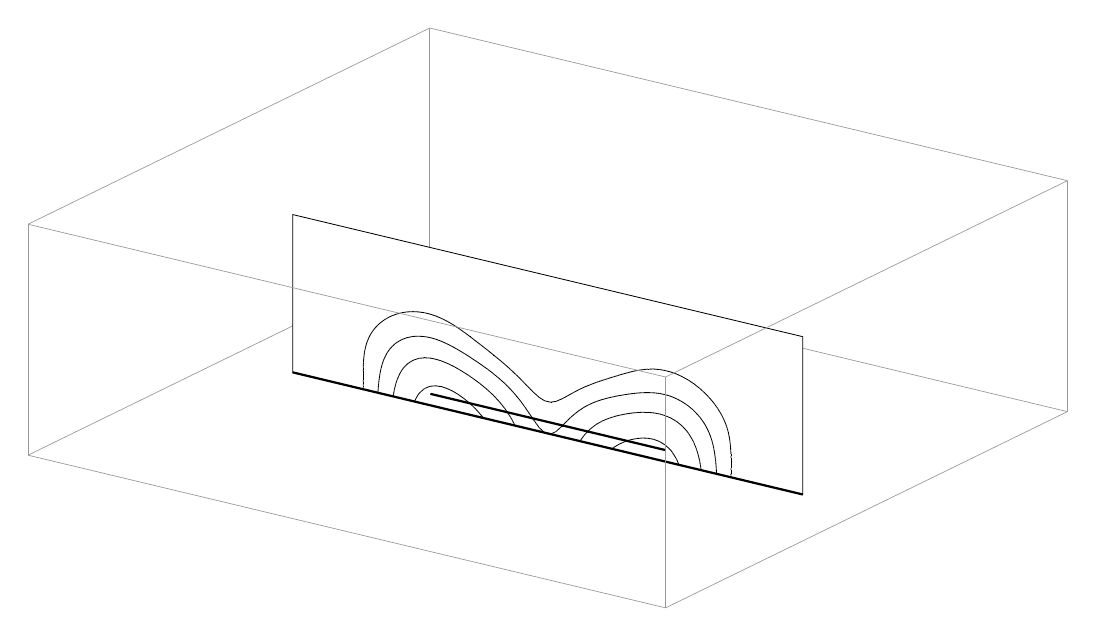
\begin{tikzpicture}
% generated by report/data/gen.py, do not edit
\draw[line width=0.25pt, black!40] (51.03mm,44.32mm) -- (51.03mm,73.64mm);
\draw[line width=0.25pt, black!40] (51.03mm,44.32mm) -- (132.00mm,24.92mm);
\draw[line width=0.25pt, black!40] (51.03mm,44.32mm) -- (25.51mm,31.85mm);
\draw[line width=0.25pt, black!40] (51.03mm,73.64mm) -- (132.00mm,54.25mm);
\draw[line width=0.25pt, black!40] (51.03mm,73.64mm) -- (25.51mm,61.18mm);
\draw[line width=0.25pt, black!40] (132.00mm,24.92mm) -- (132.00mm,54.25mm);
\draw[line width=0.25pt, black!40] (132.00mm,24.92mm) -- (106.49mm,12.46mm);
\draw[line width=0.25pt, black!40] (132.00mm,54.25mm) -- (106.49mm,41.79mm);
\filldraw[fill=white, draw=black, line width=0.30pt] (33.61mm,29.91mm) -- (98.39mm,14.40mm) -- (98.39mm,34.44mm) -- (33.61mm,49.95mm) -- cycle;
\draw[line width=0.30pt] (42.59mm,27.77mm) -- (42.58mm,27.99mm);
\draw[line width=0.30pt] (89.26mm,16.59mm) -- (89.26mm,16.81mm);
\draw[line width=0.30pt] (42.58mm,27.99mm) -- (42.58mm,28.22mm);
\draw[line width=0.30pt] (89.26mm,16.81mm) -- (89.27mm,17.04mm);
\draw[line width=0.30pt] (42.58mm,28.22mm) -- (42.57mm,28.44mm);
\draw[line width=0.30pt] (89.27mm,17.04mm) -- (89.27mm,17.26mm);
\draw[line width=0.30pt] (42.57mm,28.44mm) -- (42.57mm,28.67mm);
\draw[line width=0.30pt] (89.27mm,17.26mm) -- (89.27mm,17.48mm);
\draw[line width=0.30pt] (42.57mm,28.67mm) -- (42.56mm,28.90mm);
\draw[line width=0.30pt] (89.27mm,17.48mm) -- (89.28mm,17.71mm);
\draw[line width=0.30pt] (42.56mm,28.90mm) -- (42.56mm,29.12mm);
\draw[line width=0.30pt] (89.28mm,17.71mm) -- (89.28mm,17.93mm);
\draw[line width=0.30pt] (42.56mm,29.12mm) -- (42.56mm,29.35mm);
\draw[line width=0.30pt] (89.28mm,17.93mm) -- (89.28mm,18.16mm);
\draw[line width=0.30pt] (42.56mm,29.35mm) -- (42.56mm,29.57mm);
\draw[line width=0.30pt] (89.28mm,18.16mm) -- (89.28mm,18.38mm);
\draw[line width=0.30pt] (42.56mm,29.57mm) -- (42.56mm,29.80mm);
\draw[line width=0.30pt] (89.28mm,18.38mm) -- (89.28mm,18.61mm);
\draw[line width=0.30pt] (42.56mm,29.80mm) -- (42.56mm,30.02mm);
\draw[line width=0.30pt] (89.28mm,18.61mm) -- (89.28mm,18.83mm);
\draw[line width=0.30pt] (42.56mm,30.02mm) -- (42.57mm,30.25mm);
\draw[line width=0.30pt] (89.28mm,18.83mm) -- (89.28mm,19.06mm);
\draw[line width=0.30pt] (42.57mm,30.25mm) -- (42.57mm,30.47mm);
\draw[line width=0.30pt] (89.28mm,19.06mm) -- (89.27mm,19.29mm);
\draw[line width=0.30pt] (42.57mm,30.47mm) -- (42.58mm,30.69mm);
\draw[line width=0.30pt] (89.27mm,19.29mm) -- (89.27mm,19.51mm);
\draw[line width=0.30pt] (42.58mm,30.69mm) -- (42.59mm,30.92mm);
\draw[line width=0.30pt] (89.27mm,19.51mm) -- (89.26mm,19.74mm);
\draw[line width=0.30pt] (42.59mm,30.92mm) -- (42.60mm,31.14mm);
\draw[line width=0.30pt] (89.26mm,19.74mm) -- (89.25mm,19.97mm);
\draw[line width=0.30pt] (42.60mm,31.14mm) -- (42.61mm,31.36mm);
\draw[line width=0.30pt] (89.25mm,19.97mm) -- (89.23mm,20.20mm);
\draw[line width=0.30pt] (42.61mm,31.36mm) -- (42.63mm,31.58mm);
\draw[line width=0.30pt] (89.23mm,20.20mm) -- (89.22mm,20.43mm);
\draw[line width=0.30pt] (42.63mm,31.58mm) -- (42.65mm,31.80mm);
\draw[line width=0.30pt] (65.64mm,26.29mm) -- (65.61mm,26.30mm);
\draw[line width=0.30pt] (66.36mm,26.12mm) -- (65.64mm,26.29mm);
\draw[line width=0.30pt] (66.37mm,26.12mm) -- (66.36mm,26.12mm);
\draw[line width=0.30pt] (89.22mm,20.43mm) -- (89.20mm,20.65mm);
\draw[line width=0.30pt] (42.65mm,31.80mm) -- (42.67mm,32.02mm);
\draw[line width=0.30pt] (65.61mm,26.30mm) -- (65.01mm,26.67mm);
\draw[line width=0.30pt] (66.37mm,26.12mm) -- (66.94mm,26.21mm);
\draw[line width=0.30pt] (89.20mm,20.65mm) -- (89.17mm,20.89mm);
\draw[line width=0.30pt] (42.67mm,32.02mm) -- (42.70mm,32.24mm);
\draw[line width=0.30pt] (64.91mm,26.73mm) -- (64.63mm,26.99mm);
\draw[line width=0.30pt] (65.01mm,26.67mm) -- (64.91mm,26.73mm);
\draw[line width=0.30pt] (66.94mm,26.21mm) -- (67.09mm,26.23mm);
\draw[line width=0.30pt] (67.33mm,26.34mm) -- (67.09mm,26.23mm);
\draw[line width=0.30pt] (89.17mm,20.89mm) -- (89.15mm,21.12mm);
\draw[line width=0.30pt] (42.70mm,32.24mm) -- (42.73mm,32.46mm);
\draw[line width=0.30pt] (64.63mm,26.99mm) -- (64.28mm,27.30mm);
\draw[line width=0.30pt] (67.33mm,26.34mm) -- (67.67mm,26.49mm);
\draw[line width=0.30pt] (89.15mm,21.12mm) -- (89.11mm,21.35mm);
\draw[line width=0.30pt] (42.73mm,32.46mm) -- (42.77mm,32.67mm);
\draw[line width=0.30pt] (64.18mm,27.38mm) -- (63.98mm,27.60mm);
\draw[line width=0.30pt] (64.28mm,27.30mm) -- (64.18mm,27.38mm);
\draw[line width=0.30pt] (67.67mm,26.49mm) -- (67.82mm,26.54mm);
\draw[line width=0.30pt] (67.98mm,26.64mm) -- (67.82mm,26.54mm);
\draw[line width=0.30pt] (89.11mm,21.35mm) -- (89.08mm,21.58mm);
\draw[line width=0.30pt] (42.77mm,32.67mm) -- (42.82mm,32.89mm);
\draw[line width=0.30pt] (63.98mm,27.60mm) -- (63.69mm,27.89mm);
\draw[line width=0.30pt] (67.98mm,26.64mm) -- (68.27mm,26.79mm);
\draw[line width=0.30pt] (89.08mm,21.58mm) -- (89.03mm,21.82mm);
\draw[line width=0.30pt] (42.82mm,32.89mm) -- (42.86mm,33.10mm);
\draw[line width=0.30pt] (63.45mm,28.12mm) -- (63.39mm,28.19mm);
\draw[line width=0.30pt] (63.69mm,27.89mm) -- (63.45mm,28.12mm);
\draw[line width=0.30pt] (68.27mm,26.79mm) -- (68.55mm,26.94mm);
\draw[line width=0.30pt] (68.56mm,26.95mm) -- (68.55mm,26.94mm);
\draw[line width=0.30pt] (89.03mm,21.82mm) -- (88.98mm,22.06mm);
\draw[line width=0.30pt] (42.86mm,33.10mm) -- (42.92mm,33.31mm);
\draw[line width=0.30pt] (63.39mm,28.19mm) -- (63.11mm,28.48mm);
\draw[line width=0.30pt] (68.56mm,26.95mm) -- (68.84mm,27.11mm);
\draw[line width=0.30pt] (88.93mm,22.29mm) -- (88.93mm,22.30mm);
\draw[line width=0.30pt] (88.98mm,22.06mm) -- (88.93mm,22.29mm);
\draw[line width=0.30pt] (42.92mm,33.31mm) -- (42.98mm,33.52mm);
\draw[line width=0.30pt] (63.11mm,28.48mm) -- (62.83mm,28.77mm);
\draw[line width=0.30pt] (68.84mm,27.11mm) -- (69.12mm,27.26mm);
\draw[line width=0.30pt] (88.93mm,22.30mm) -- (88.87mm,22.54mm);
\draw[line width=0.30pt] (42.98mm,33.52mm) -- (43.05mm,33.73mm);
\draw[line width=0.30pt] (62.72mm,28.87mm) -- (62.54mm,29.07mm);
\draw[line width=0.30pt] (62.83mm,28.77mm) -- (62.72mm,28.87mm);
\draw[line width=0.30pt] (69.12mm,27.26mm) -- (69.28mm,27.35mm);
\draw[line width=0.30pt] (69.41mm,27.42mm) -- (69.28mm,27.35mm);
\draw[line width=0.30pt] (88.87mm,22.54mm) -- (88.80mm,22.78mm);
\draw[line width=0.30pt] (43.05mm,33.73mm) -- (43.07mm,33.79mm);
\draw[line width=0.30pt] (43.13mm,33.94mm) -- (43.07mm,33.79mm);
\draw[line width=0.30pt] (62.54mm,29.07mm) -- (62.24mm,29.36mm);
\draw[line width=0.30pt] (69.41mm,27.42mm) -- (69.70mm,27.57mm);
\draw[line width=0.30pt] (88.80mm,22.78mm) -- (88.72mm,23.02mm);
\draw[line width=0.30pt] (43.13mm,33.94mm) -- (43.21mm,34.14mm);
\draw[line width=0.30pt] (62.00mm,29.60mm) -- (61.93mm,29.66mm);
\draw[line width=0.30pt] (62.24mm,29.36mm) -- (62.00mm,29.60mm);
\draw[line width=0.30pt] (69.70mm,27.57mm) -- (70.00mm,27.73mm);
\draw[line width=0.30pt] (70.00mm,27.73mm) -- (70.00mm,27.73mm);
\draw[line width=0.30pt] (88.72mm,23.02mm) -- (88.64mm,23.27mm);
\draw[line width=0.30pt] (43.21mm,34.14mm) -- (43.30mm,34.35mm);
\draw[line width=0.30pt] (61.93mm,29.66mm) -- (61.62mm,29.96mm);
\draw[line width=0.30pt] (70.00mm,27.73mm) -- (70.32mm,27.88mm);
\draw[line width=0.30pt] (88.64mm,23.27mm) -- (88.54mm,23.51mm);
\draw[line width=0.30pt] (43.30mm,34.35mm) -- (43.40mm,34.55mm);
\draw[line width=0.30pt] (61.62mm,29.96mm) -- (61.29mm,30.26mm);
\draw[line width=0.30pt] (70.32mm,27.88mm) -- (70.64mm,28.03mm);
\draw[line width=0.30pt] (88.54mm,23.51mm) -- (88.44mm,23.76mm);
\draw[line width=0.30pt] (43.40mm,34.55mm) -- (43.51mm,34.75mm);
\draw[line width=0.30pt] (61.27mm,30.29mm) -- (60.95mm,30.57mm);
\draw[line width=0.30pt] (61.29mm,30.26mm) -- (61.27mm,30.29mm);
\draw[line width=0.30pt] (70.64mm,28.03mm) -- (70.73mm,28.07mm);
\draw[line width=0.30pt] (70.98mm,28.17mm) -- (70.73mm,28.07mm);
\draw[line width=0.30pt] (88.44mm,23.76mm) -- (88.33mm,24.02mm);
\draw[line width=0.30pt] (43.51mm,34.75mm) -- (43.63mm,34.94mm);
\draw[line width=0.30pt] (60.95mm,30.57mm) -- (60.61mm,30.88mm);
\draw[line width=0.30pt] (70.98mm,28.17mm) -- (71.33mm,28.31mm);
\draw[line width=0.30pt] (88.33mm,24.02mm) -- (88.20mm,24.27mm);
\draw[line width=0.30pt] (43.63mm,34.94mm) -- (43.76mm,35.14mm);
\draw[line width=0.30pt] (60.54mm,30.94mm) -- (60.24mm,31.19mm);
\draw[line width=0.30pt] (60.61mm,30.88mm) -- (60.54mm,30.94mm);
\draw[line width=0.30pt] (71.33mm,28.31mm) -- (71.46mm,28.37mm);
\draw[line width=0.30pt] (71.69mm,28.45mm) -- (71.46mm,28.37mm);
\draw[line width=0.30pt] (88.20mm,24.27mm) -- (88.07mm,24.53mm);
\draw[line width=0.30pt] (88.20mm,24.27mm) -- (88.20mm,24.27mm);
\draw[line width=0.30pt] (43.76mm,35.14mm) -- (43.80mm,35.19mm);
\draw[line width=0.30pt] (43.90mm,35.33mm) -- (43.80mm,35.19mm);
\draw[line width=0.30pt] (60.24mm,31.19mm) -- (59.87mm,31.51mm);
\draw[line width=0.30pt] (71.69mm,28.45mm) -- (72.05mm,28.59mm);
\draw[line width=0.30pt] (88.07mm,24.53mm) -- (87.92mm,24.79mm);
\draw[line width=0.30pt] (43.90mm,35.33mm) -- (44.06mm,35.52mm);
\draw[line width=0.30pt] (59.81mm,31.55mm) -- (59.48mm,31.82mm);
\draw[line width=0.30pt] (59.87mm,31.51mm) -- (59.81mm,31.55mm);
\draw[line width=0.30pt] (72.05mm,28.59mm) -- (72.19mm,28.64mm);
\draw[line width=0.30pt] (72.44mm,28.72mm) -- (72.19mm,28.64mm);
\draw[line width=0.30pt] (87.92mm,24.79mm) -- (87.76mm,25.05mm);
\draw[line width=0.30pt] (44.06mm,35.52mm) -- (44.22mm,35.70mm);
\draw[line width=0.30pt] (59.48mm,31.82mm) -- (59.09mm,32.14mm);
\draw[line width=0.30pt] (72.44mm,28.72mm) -- (72.82mm,28.85mm);
\draw[line width=0.30pt] (87.76mm,25.05mm) -- (87.59mm,25.32mm);
\draw[line width=0.30pt] (44.22mm,35.70mm) -- (44.40mm,35.89mm);
\draw[line width=0.30pt] (59.09mm,32.15mm) -- (58.68mm,32.47mm);
\draw[line width=0.30pt] (59.09mm,32.14mm) -- (59.09mm,32.15mm);
\draw[line width=0.30pt] (72.82mm,28.85mm) -- (72.91mm,28.89mm);
\draw[line width=0.30pt] (73.22mm,28.98mm) -- (72.91mm,28.89mm);
\draw[line width=0.30pt] (87.47mm,25.49mm) -- (87.40mm,25.59mm);
\draw[line width=0.30pt] (87.59mm,25.32mm) -- (87.47mm,25.49mm);
\draw[line width=0.30pt] (44.40mm,35.89mm) -- (44.53mm,36.01mm);
\draw[line width=0.30pt] (44.59mm,36.07mm) -- (44.53mm,36.01mm);
\draw[line width=0.30pt] (58.36mm,32.73mm) -- (58.28mm,32.79mm);
\draw[line width=0.30pt] (58.68mm,32.47mm) -- (58.36mm,32.73mm);
\draw[line width=0.30pt] (73.22mm,28.98mm) -- (73.62mm,29.11mm);
\draw[line width=0.30pt] (87.40mm,25.59mm) -- (87.20mm,25.86mm);
\draw[line width=0.30pt] (44.59mm,36.07mm) -- (44.80mm,36.24mm);
\draw[line width=0.30pt] (58.28mm,32.79mm) -- (57.86mm,33.11mm);
\draw[line width=0.30pt] (73.62mm,29.11mm) -- (73.64mm,29.12mm);
\draw[line width=0.30pt] (74.04mm,29.24mm) -- (73.64mm,29.12mm);
\draw[line width=0.30pt] (87.20mm,25.86mm) -- (86.99mm,26.14mm);
\draw[line width=0.30pt] (44.80mm,36.24mm) -- (45.02mm,36.41mm);
\draw[line width=0.30pt] (57.63mm,33.30mm) -- (57.45mm,33.44mm);
\draw[line width=0.30pt] (57.86mm,33.11mm) -- (57.63mm,33.30mm);
\draw[line width=0.30pt] (74.04mm,29.24mm) -- (74.37mm,29.35mm);
\draw[line width=0.30pt] (74.44mm,29.37mm) -- (74.37mm,29.35mm);
\draw[line width=0.30pt] (86.99mm,26.14mm) -- (86.76mm,26.42mm);
\draw[line width=0.30pt] (45.02mm,36.41mm) -- (45.26mm,36.58mm);
\draw[line width=0.30pt] (45.26mm,36.58mm) -- (45.26mm,36.58mm);
\draw[line width=0.30pt] (57.45mm,33.44mm) -- (57.03mm,33.76mm);
\draw[line width=0.30pt] (74.44mm,29.37mm) -- (74.86mm,29.49mm);
\draw[line width=0.30pt] (86.74mm,26.44mm) -- (86.51mm,26.70mm);
\draw[line width=0.30pt] (86.76mm,26.42mm) -- (86.74mm,26.44mm);
\draw[line width=0.30pt] (45.26mm,36.58mm) -- (45.52mm,36.74mm);
\draw[line width=0.30pt] (56.90mm,33.86mm) -- (56.60mm,34.09mm);
\draw[line width=0.30pt] (57.03mm,33.76mm) -- (56.90mm,33.86mm);
\draw[line width=0.30pt] (74.86mm,29.49mm) -- (75.10mm,29.57mm);
\draw[line width=0.30pt] (75.28mm,29.62mm) -- (75.10mm,29.57mm);
\draw[line width=0.30pt] (86.51mm,26.70mm) -- (86.24mm,26.99mm);
\draw[line width=0.30pt] (45.52mm,36.74mm) -- (45.81mm,36.90mm);
\draw[line width=0.30pt] (56.60mm,34.09mm) -- (56.18mm,34.42mm);
\draw[line width=0.30pt] (75.28mm,29.62mm) -- (75.71mm,29.74mm);
\draw[line width=0.30pt] (86.02mm,27.22mm) -- (85.94mm,27.29mm);
\draw[line width=0.30pt] (86.24mm,26.99mm) -- (86.02mm,27.22mm);
\draw[line width=0.30pt] (45.81mm,36.90mm) -- (45.98mm,36.99mm);
\draw[line width=0.30pt] (46.12mm,37.05mm) -- (45.98mm,36.99mm);
\draw[line width=0.30pt] (56.17mm,34.42mm) -- (55.73mm,34.75mm);
\draw[line width=0.30pt] (56.18mm,34.42mm) -- (56.17mm,34.42mm);
\draw[line width=0.30pt] (75.71mm,29.74mm) -- (75.83mm,29.78mm);
\draw[line width=0.30pt] (76.15mm,29.86mm) -- (75.83mm,29.78mm);
\draw[line width=0.30pt] (85.94mm,27.29mm) -- (85.62mm,27.59mm);
\draw[line width=0.30pt] (46.12mm,37.05mm) -- (46.47mm,37.19mm);
\draw[line width=0.30pt] (55.45mm,34.96mm) -- (55.28mm,35.08mm);
\draw[line width=0.30pt] (55.73mm,34.75mm) -- (55.45mm,34.96mm);
\draw[line width=0.30pt] (76.15mm,29.86mm) -- (76.55mm,29.97mm);
\draw[line width=0.30pt] (76.60mm,29.98mm) -- (76.55mm,29.97mm);
\draw[line width=0.30pt] (85.29mm,27.89mm) -- (85.27mm,27.90mm);
\draw[line width=0.30pt] (85.62mm,27.59mm) -- (85.29mm,27.89mm);
\draw[line width=0.30pt] (46.47mm,37.19mm) -- (46.71mm,37.28mm);
\draw[line width=0.30pt] (46.86mm,37.32mm) -- (46.71mm,37.28mm);
\draw[line width=0.30pt] (55.28mm,35.08mm) -- (54.80mm,35.42mm);
\draw[line width=0.30pt] (76.60mm,29.98mm) -- (77.08mm,30.09mm);
\draw[line width=0.30pt] (85.27mm,27.90mm) -- (84.87mm,28.22mm);
\draw[line width=0.30pt] (46.86mm,37.32mm) -- (47.30mm,37.44mm);
\draw[line width=0.30pt] (54.72mm,35.48mm) -- (54.27mm,35.77mm);
\draw[line width=0.30pt] (54.80mm,35.42mm) -- (54.72mm,35.48mm);
\draw[line width=0.30pt] (77.08mm,30.09mm) -- (77.28mm,30.13mm);
\draw[line width=0.30pt] (77.61mm,30.18mm) -- (77.28mm,30.13mm);
\draw[line width=0.30pt] (84.56mm,28.46mm) -- (84.42mm,28.55mm);
\draw[line width=0.30pt] (84.87mm,28.22mm) -- (84.56mm,28.46mm);
\draw[line width=0.30pt] (47.30mm,37.44mm) -- (47.44mm,37.48mm);
\draw[line width=0.30pt] (47.84mm,37.54mm) -- (47.44mm,37.48mm);
\draw[line width=0.30pt] (53.99mm,35.96mm) -- (53.68mm,36.14mm);
\draw[line width=0.30pt] (54.27mm,35.77mm) -- (53.99mm,35.96mm);
\draw[line width=0.30pt] (77.61mm,30.18mm) -- (78.01mm,30.25mm);
\draw[line width=0.30pt] (78.20mm,30.27mm) -- (78.01mm,30.25mm);
\draw[line width=0.30pt] (84.42mm,28.55mm) -- (83.89mm,28.90mm);
\draw[line width=0.30pt] (47.84mm,37.54mm) -- (48.17mm,37.59mm);
\draw[line width=0.30pt] (48.51mm,37.60mm) -- (48.17mm,37.59mm);
\draw[line width=0.30pt] (53.26mm,36.38mm) -- (52.96mm,36.54mm);
\draw[line width=0.30pt] (53.68mm,36.14mm) -- (53.26mm,36.38mm);
\draw[line width=0.30pt] (78.20mm,30.27mm) -- (78.74mm,30.32mm);
\draw[line width=0.30pt] (78.92mm,30.32mm) -- (78.74mm,30.32mm);
\draw[line width=0.30pt] (83.83mm,28.94mm) -- (83.21mm,29.29mm);
\draw[line width=0.30pt] (83.89mm,28.90mm) -- (83.83mm,28.94mm);
\draw[line width=0.30pt] (48.51mm,37.60mm) -- (48.90mm,37.62mm);
\draw[line width=0.30pt] (49.51mm,37.59mm) -- (48.90mm,37.62mm);
\draw[line width=0.30pt] (52.53mm,36.75mm) -- (51.93mm,37.01mm);
\draw[line width=0.30pt] (52.96mm,36.54mm) -- (52.53mm,36.75mm);
\draw[line width=0.30pt] (78.92mm,30.32mm) -- (79.47mm,30.33mm);
\draw[line width=0.30pt] (80.02mm,30.28mm) -- (79.47mm,30.33mm);
\draw[line width=0.30pt] (82.38mm,29.69mm) -- (82.11mm,29.78mm);
\draw[line width=0.30pt] (83.10mm,29.35mm) -- (82.38mm,29.69mm);
\draw[line width=0.30pt] (83.21mm,29.29mm) -- (83.10mm,29.35mm);
\draw[line width=0.30pt] (49.51mm,37.59mm) -- (49.62mm,37.58mm);
\draw[line width=0.30pt] (50.35mm,37.48mm) -- (49.62mm,37.58mm);
\draw[line width=0.30pt] (51.08mm,37.30mm) -- (50.35mm,37.48mm);
\draw[line width=0.30pt] (51.81mm,37.06mm) -- (51.08mm,37.30mm);
\draw[line width=0.30pt] (51.93mm,37.01mm) -- (51.81mm,37.06mm);
\draw[line width=0.30pt] (80.02mm,30.28mm) -- (80.19mm,30.27mm);
\draw[line width=0.30pt] (80.92mm,30.14mm) -- (80.19mm,30.27mm);
\draw[line width=0.30pt] (81.65mm,29.95mm) -- (80.92mm,30.14mm);
\draw[line width=0.30pt] (82.11mm,29.78mm) -- (81.65mm,29.95mm);
\draw[line width=0.30pt] (44.44mm,27.32mm) -- (44.45mm,27.54mm);
\draw[line width=0.30pt] (65.59mm,22.26mm) -- (65.28mm,22.56mm);
\draw[line width=0.30pt] (66.39mm,22.06mm) -- (66.69mm,22.22mm);
\draw[line width=0.30pt] (87.44mm,17.02mm) -- (87.43mm,17.25mm);
\draw[line width=0.30pt] (44.45mm,27.54mm) -- (44.47mm,27.76mm);
\draw[line width=0.30pt] (65.28mm,22.56mm) -- (64.95mm,22.86mm);
\draw[line width=0.30pt] (66.69mm,22.22mm) -- (67.00mm,22.37mm);
\draw[line width=0.30pt] (87.43mm,17.25mm) -- (87.42mm,17.48mm);
\draw[line width=0.30pt] (44.47mm,27.76mm) -- (44.49mm,27.99mm);
\draw[line width=0.30pt] (64.91mm,22.90mm) -- (64.75mm,23.13mm);
\draw[line width=0.30pt] (64.95mm,22.86mm) -- (64.91mm,22.90mm);
\draw[line width=0.30pt] (67.00mm,22.37mm) -- (67.09mm,22.41mm);
\draw[line width=0.30pt] (67.22mm,22.54mm) -- (67.09mm,22.41mm);
\draw[line width=0.30pt] (87.42mm,17.48mm) -- (87.40mm,17.71mm);
\draw[line width=0.30pt] (44.49mm,27.99mm) -- (44.50mm,28.21mm);
\draw[line width=0.30pt] (64.75mm,23.13mm) -- (64.55mm,23.40mm);
\draw[line width=0.30pt] (67.22mm,22.54mm) -- (67.41mm,22.72mm);
\draw[line width=0.30pt] (87.40mm,17.71mm) -- (87.39mm,17.94mm);
\draw[line width=0.30pt] (44.50mm,28.21mm) -- (44.52mm,28.43mm);
\draw[line width=0.30pt] (64.55mm,23.40mm) -- (64.35mm,23.68mm);
\draw[line width=0.30pt] (67.41mm,22.72mm) -- (67.61mm,22.90mm);
\draw[line width=0.30pt] (87.39mm,17.94mm) -- (87.37mm,18.17mm);
\draw[line width=0.30pt] (44.52mm,28.43mm) -- (44.53mm,28.47mm);
\draw[line width=0.30pt] (44.55mm,28.65mm) -- (44.53mm,28.47mm);
\draw[line width=0.30pt] (64.18mm,23.91mm) -- (64.15mm,23.95mm);
\draw[line width=0.30pt] (64.35mm,23.68mm) -- (64.18mm,23.91mm);
\draw[line width=0.30pt] (67.61mm,22.90mm) -- (67.81mm,23.08mm);
\draw[line width=0.30pt] (87.37mm,18.17mm) -- (87.35mm,18.40mm);
\draw[line width=0.30pt] (44.55mm,28.65mm) -- (44.57mm,28.87mm);
\draw[line width=0.30pt] (64.15mm,23.95mm) -- (63.98mm,24.22mm);
\draw[line width=0.30pt] (67.81mm,23.08mm) -- (67.82mm,23.08mm);
\draw[line width=0.30pt] (67.98mm,23.26mm) -- (67.82mm,23.08mm);
\draw[line width=0.30pt] (87.35mm,18.40mm) -- (87.33mm,18.63mm);
\draw[line width=0.30pt] (44.57mm,28.87mm) -- (44.60mm,29.08mm);
\draw[line width=0.30pt] (63.98mm,24.22mm) -- (63.80mm,24.48mm);
\draw[line width=0.30pt] (67.98mm,23.26mm) -- (68.16mm,23.44mm);
\draw[line width=0.30pt] (87.33mm,18.63mm) -- (87.30mm,18.86mm);
\draw[line width=0.30pt] (44.60mm,29.08mm) -- (44.63mm,29.30mm);
\draw[line width=0.30pt] (63.80mm,24.48mm) -- (63.62mm,24.75mm);
\draw[line width=0.30pt] (68.16mm,23.44mm) -- (68.34mm,23.62mm);
\draw[line width=0.30pt] (87.30mm,18.86mm) -- (87.27mm,19.09mm);
\draw[line width=0.30pt] (44.63mm,29.30mm) -- (44.66mm,29.52mm);
\draw[line width=0.30pt] (63.45mm,24.99mm) -- (63.43mm,25.02mm);
\draw[line width=0.30pt] (63.62mm,24.75mm) -- (63.45mm,24.99mm);
\draw[line width=0.30pt] (68.34mm,23.62mm) -- (68.53mm,23.80mm);
\draw[line width=0.30pt] (87.27mm,19.09mm) -- (87.24mm,19.32mm);
\draw[line width=0.30pt] (44.66mm,29.52mm) -- (44.70mm,29.74mm);
\draw[line width=0.30pt] (63.43mm,25.02mm) -- (63.25mm,25.29mm);
\draw[line width=0.30pt] (68.53mm,23.80mm) -- (68.55mm,23.82mm);
\draw[line width=0.30pt] (68.71mm,23.99mm) -- (68.55mm,23.82mm);
\draw[line width=0.30pt] (87.24mm,19.32mm) -- (87.21mm,19.56mm);
\draw[line width=0.30pt] (44.70mm,29.74mm) -- (44.74mm,29.95mm);
\draw[line width=0.30pt] (63.25mm,25.29mm) -- (63.06mm,25.56mm);
\draw[line width=0.30pt] (68.71mm,23.99mm) -- (68.90mm,24.17mm);
\draw[line width=0.30pt] (87.21mm,19.56mm) -- (87.17mm,19.79mm);
\draw[line width=0.30pt] (44.74mm,29.95mm) -- (44.78mm,30.17mm);
\draw[line width=0.30pt] (63.06mm,25.56mm) -- (62.86mm,25.84mm);
\draw[line width=0.30pt] (68.90mm,24.17mm) -- (69.09mm,24.34mm);
\draw[line width=0.30pt] (87.17mm,19.79mm) -- (87.13mm,20.02mm);
\draw[line width=0.30pt] (44.78mm,30.17mm) -- (44.83mm,30.38mm);
\draw[line width=0.30pt] (62.72mm,26.02mm) -- (62.66mm,26.11mm);
\draw[line width=0.30pt] (62.86mm,25.84mm) -- (62.72mm,26.02mm);
\draw[line width=0.30pt] (69.09mm,24.34mm) -- (69.28mm,24.50mm);
\draw[line width=0.30pt] (69.30mm,24.52mm) -- (69.28mm,24.50mm);
\draw[line width=0.30pt] (87.13mm,20.02mm) -- (87.09mm,20.26mm);
\draw[line width=0.30pt] (44.83mm,30.38mm) -- (44.88mm,30.59mm);
\draw[line width=0.30pt] (62.66mm,26.11mm) -- (62.45mm,26.39mm);
\draw[line width=0.30pt] (69.30mm,24.52mm) -- (69.51mm,24.69mm);
\draw[line width=0.30pt] (87.09mm,20.26mm) -- (87.04mm,20.50mm);
\draw[line width=0.30pt] (44.88mm,30.59mm) -- (44.94mm,30.80mm);
\draw[line width=0.30pt] (62.45mm,26.39mm) -- (62.23mm,26.66mm);
\draw[line width=0.30pt] (69.51mm,24.69mm) -- (69.73mm,24.87mm);
\draw[line width=0.30pt] (87.04mm,20.50mm) -- (86.98mm,20.74mm);
\draw[line width=0.30pt] (44.94mm,30.80mm) -- (45.00mm,31.01mm);
\draw[line width=0.30pt] (62.23mm,26.66mm) -- (62.00mm,26.94mm);
\draw[line width=0.30pt] (69.73mm,24.87mm) -- (69.95mm,25.04mm);
\draw[line width=0.30pt] (86.98mm,20.74mm) -- (86.92mm,20.97mm);
\draw[line width=0.30pt] (45.00mm,31.01mm) -- (45.07mm,31.22mm);
\draw[line width=0.30pt] (62.00mm,26.95mm) -- (61.75mm,27.23mm);
\draw[line width=0.30pt] (62.00mm,26.94mm) -- (62.00mm,26.95mm);
\draw[line width=0.30pt] (69.95mm,25.04mm) -- (70.00mm,25.07mm);
\draw[line width=0.30pt] (70.20mm,25.20mm) -- (70.00mm,25.07mm);
\draw[line width=0.30pt] (86.92mm,20.97mm) -- (86.86mm,21.22mm);
\draw[line width=0.30pt] (45.07mm,31.22mm) -- (45.14mm,31.43mm);
\draw[line width=0.30pt] (61.75mm,27.23mm) -- (61.50mm,27.51mm);
\draw[line width=0.30pt] (70.20mm,25.20mm) -- (70.45mm,25.37mm);
\draw[line width=0.30pt] (86.86mm,21.22mm) -- (86.78mm,21.46mm);
\draw[line width=0.30pt] (45.14mm,31.43mm) -- (45.23mm,31.64mm);
\draw[line width=0.30pt] (61.27mm,27.77mm) -- (61.24mm,27.80mm);
\draw[line width=0.30pt] (61.50mm,27.51mm) -- (61.27mm,27.77mm);
\draw[line width=0.30pt] (70.45mm,25.37mm) -- (70.72mm,25.53mm);
\draw[line width=0.30pt] (86.74mm,21.58mm) -- (86.70mm,21.70mm);
\draw[line width=0.30pt] (86.78mm,21.46mm) -- (86.74mm,21.58mm);
\draw[line width=0.30pt] (45.23mm,31.64mm) -- (45.26mm,31.71mm);
\draw[line width=0.30pt] (45.32mm,31.84mm) -- (45.26mm,31.71mm);
\draw[line width=0.30pt] (61.24mm,27.80mm) -- (60.95mm,28.10mm);
\draw[line width=0.30pt] (70.72mm,25.53mm) -- (70.73mm,25.54mm);
\draw[line width=0.30pt] (71.01mm,25.69mm) -- (70.73mm,25.54mm);
\draw[line width=0.30pt] (86.70mm,21.70mm) -- (86.61mm,21.95mm);
\draw[line width=0.30pt] (45.32mm,31.84mm) -- (45.42mm,32.04mm);
\draw[line width=0.30pt] (60.95mm,28.10mm) -- (60.65mm,28.39mm);
\draw[line width=0.30pt] (71.01mm,25.69mm) -- (71.31mm,25.84mm);
\draw[line width=0.30pt] (86.61mm,21.95mm) -- (86.51mm,22.20mm);
\draw[line width=0.30pt] (45.42mm,32.04mm) -- (45.52mm,32.24mm);
\draw[line width=0.30pt] (60.54mm,28.50mm) -- (60.32mm,28.70mm);
\draw[line width=0.30pt] (60.65mm,28.39mm) -- (60.54mm,28.50mm);
\draw[line width=0.30pt] (71.31mm,25.84mm) -- (71.46mm,25.91mm);
\draw[line width=0.30pt] (71.63mm,25.99mm) -- (71.46mm,25.91mm);
\draw[line width=0.30pt] (86.51mm,22.20mm) -- (86.40mm,22.45mm);
\draw[line width=0.30pt] (45.52mm,32.24mm) -- (45.64mm,32.44mm);
\draw[line width=0.30pt] (60.32mm,28.70mm) -- (59.98mm,29.00mm);
\draw[line width=0.30pt] (71.63mm,25.99mm) -- (71.98mm,26.13mm);
\draw[line width=0.30pt] (86.40mm,22.45mm) -- (86.28mm,22.70mm);
\draw[line width=0.30pt] (45.64mm,32.44mm) -- (45.77mm,32.63mm);
\draw[line width=0.30pt] (59.81mm,29.15mm) -- (59.62mm,29.31mm);
\draw[line width=0.30pt] (59.98mm,29.00mm) -- (59.81mm,29.15mm);
\draw[line width=0.30pt] (71.98mm,26.13mm) -- (72.19mm,26.21mm);
\draw[line width=0.30pt] (72.35mm,26.27mm) -- (72.19mm,26.21mm);
\draw[line width=0.30pt] (86.28mm,22.70mm) -- (86.15mm,22.96mm);
\draw[line width=0.30pt] (45.77mm,32.63mm) -- (45.91mm,32.82mm);
\draw[line width=0.30pt] (59.62mm,29.31mm) -- (59.23mm,29.63mm);
\draw[line width=0.30pt] (72.35mm,26.27mm) -- (72.74mm,26.40mm);
\draw[line width=0.30pt] (86.02mm,23.20mm) -- (86.01mm,23.22mm);
\draw[line width=0.30pt] (86.15mm,22.96mm) -- (86.02mm,23.20mm);
\draw[line width=0.30pt] (45.91mm,32.82mm) -- (45.98mm,32.92mm);
\draw[line width=0.30pt] (46.07mm,33.01mm) -- (45.98mm,32.92mm);
\draw[line width=0.30pt] (59.09mm,29.75mm) -- (58.82mm,29.96mm);
\draw[line width=0.30pt] (59.23mm,29.63mm) -- (59.09mm,29.75mm);
\draw[line width=0.30pt] (72.74mm,26.40mm) -- (72.91mm,26.45mm);
\draw[line width=0.30pt] (73.16mm,26.52mm) -- (72.91mm,26.45mm);
\draw[line width=0.30pt] (86.01mm,23.22mm) -- (85.84mm,23.49mm);
\draw[line width=0.30pt] (46.07mm,33.01mm) -- (46.24mm,33.19mm);
\draw[line width=0.30pt] (58.82mm,29.96mm) -- (58.39mm,30.28mm);
\draw[line width=0.30pt] (73.16mm,26.52mm) -- (73.60mm,26.64mm);
\draw[line width=0.30pt] (85.84mm,23.49mm) -- (85.66mm,23.75mm);
\draw[line width=0.30pt] (46.24mm,33.19mm) -- (46.43mm,33.37mm);
\draw[line width=0.30pt] (58.36mm,30.31mm) -- (57.92mm,30.62mm);
\draw[line width=0.30pt] (58.39mm,30.28mm) -- (58.36mm,30.31mm);
\draw[line width=0.30pt] (73.60mm,26.64mm) -- (73.64mm,26.65mm);
\draw[line width=0.30pt] (74.08mm,26.75mm) -- (73.64mm,26.65mm);
\draw[line width=0.30pt] (85.66mm,23.75mm) -- (85.46mm,24.03mm);
\draw[line width=0.30pt] (46.43mm,33.37mm) -- (46.63mm,33.55mm);
\draw[line width=0.30pt] (57.63mm,30.83mm) -- (57.44mm,30.96mm);
\draw[line width=0.30pt] (57.92mm,30.62mm) -- (57.63mm,30.83mm);
\draw[line width=0.30pt] (74.08mm,26.75mm) -- (74.37mm,26.82mm);
\draw[line width=0.30pt] (74.57mm,26.86mm) -- (74.37mm,26.82mm);
\draw[line width=0.30pt] (85.29mm,24.26mm) -- (85.25mm,24.30mm);
\draw[line width=0.30pt] (85.46mm,24.03mm) -- (85.29mm,24.26mm);
\draw[line width=0.30pt] (46.63mm,33.55mm) -- (46.71mm,33.62mm);
\draw[line width=0.30pt] (46.87mm,33.72mm) -- (46.71mm,33.62mm);
\draw[line width=0.30pt] (57.44mm,30.96mm) -- (56.94mm,31.31mm);
\draw[line width=0.30pt] (74.57mm,26.86mm) -- (75.09mm,26.96mm);
\draw[line width=0.30pt] (85.25mm,24.30mm) -- (84.99mm,24.59mm);
\draw[line width=0.30pt] (46.87mm,33.72mm) -- (47.13mm,33.88mm);
\draw[line width=0.30pt] (56.90mm,31.33mm) -- (56.41mm,31.66mm);
\draw[line width=0.30pt] (56.94mm,31.31mm) -- (56.90mm,31.33mm);
\draw[line width=0.30pt] (75.09mm,26.96mm) -- (75.10mm,26.96mm);
\draw[line width=0.30pt] (75.64mm,27.05mm) -- (75.10mm,26.96mm);
\draw[line width=0.30pt] (84.99mm,24.59mm) -- (84.72mm,24.88mm);
\draw[line width=0.30pt] (47.13mm,33.88mm) -- (47.41mm,34.04mm);
\draw[line width=0.30pt] (56.17mm,31.82mm) -- (55.86mm,32.02mm);
\draw[line width=0.30pt] (56.41mm,31.66mm) -- (56.17mm,31.82mm);
\draw[line width=0.30pt] (75.64mm,27.05mm) -- (75.83mm,27.08mm);
\draw[line width=0.30pt] (76.22mm,27.14mm) -- (75.83mm,27.08mm);
\draw[line width=0.30pt] (84.56mm,25.04mm) -- (84.41mm,25.18mm);
\draw[line width=0.30pt] (84.72mm,24.88mm) -- (84.56mm,25.04mm);
\draw[line width=0.30pt] (47.41mm,34.04mm) -- (47.44mm,34.06mm);
\draw[line width=0.30pt] (47.76mm,34.18mm) -- (47.44mm,34.06mm);
\draw[line width=0.30pt] (55.45mm,32.28mm) -- (55.28mm,32.38mm);
\draw[line width=0.30pt] (55.86mm,32.02mm) -- (55.45mm,32.28mm);
\draw[line width=0.30pt] (76.22mm,27.14mm) -- (76.55mm,27.19mm);
\draw[line width=0.30pt] (76.83mm,27.22mm) -- (76.55mm,27.19mm);
\draw[line width=0.30pt] (84.41mm,25.18mm) -- (84.04mm,25.49mm);
\draw[line width=0.30pt] (47.76mm,34.18mm) -- (48.14mm,34.32mm);
\draw[line width=0.30pt] (54.72mm,32.72mm) -- (54.67mm,32.75mm);
\draw[line width=0.30pt] (55.28mm,32.38mm) -- (54.72mm,32.72mm);
\draw[line width=0.30pt] (76.83mm,27.22mm) -- (77.28mm,27.27mm);
\draw[line width=0.30pt] (77.49mm,27.29mm) -- (77.28mm,27.27mm);
\draw[line width=0.30pt] (83.83mm,25.66mm) -- (83.61mm,25.82mm);
\draw[line width=0.30pt] (84.04mm,25.49mm) -- (83.83mm,25.66mm);
\draw[line width=0.30pt] (48.14mm,34.32mm) -- (48.17mm,34.32mm);
\draw[line width=0.30pt] (48.64mm,34.42mm) -- (48.17mm,34.32mm);
\draw[line width=0.30pt] (53.99mm,33.13mm) -- (53.98mm,33.14mm);
\draw[line width=0.30pt] (54.67mm,32.75mm) -- (53.99mm,33.13mm);
\draw[line width=0.30pt] (77.49mm,27.29mm) -- (78.01mm,27.32mm);
\draw[line width=0.30pt] (78.25mm,27.33mm) -- (78.01mm,27.32mm);
\draw[line width=0.30pt] (83.10mm,26.16mm) -- (83.08mm,26.17mm);
\draw[line width=0.30pt] (83.61mm,25.82mm) -- (83.10mm,26.16mm);
\draw[line width=0.30pt] (48.64mm,34.42mm) -- (48.90mm,34.47mm);
\draw[line width=0.30pt] (49.29mm,34.49mm) -- (48.90mm,34.47mm);
\draw[line width=0.30pt] (53.26mm,33.51mm) -- (53.13mm,33.57mm);
\draw[line width=0.30pt] (53.98mm,33.14mm) -- (53.26mm,33.51mm);
\draw[line width=0.30pt] (78.25mm,27.33mm) -- (78.74mm,27.34mm);
\draw[line width=0.30pt] (79.21mm,27.32mm) -- (78.74mm,27.34mm);
\draw[line width=0.30pt] (82.38mm,26.55mm) -- (82.31mm,26.58mm);
\draw[line width=0.30pt] (83.08mm,26.17mm) -- (82.38mm,26.55mm);
\draw[line width=0.30pt] (49.29mm,34.49mm) -- (49.62mm,34.50mm);
\draw[line width=0.30pt] (50.35mm,34.45mm) -- (49.62mm,34.50mm);
\draw[line width=0.30pt] (50.54mm,34.42mm) -- (50.35mm,34.45mm);
\draw[line width=0.30pt] (51.81mm,34.11mm) -- (51.75mm,34.13mm);
\draw[line width=0.30pt] (52.53mm,33.84mm) -- (51.81mm,34.11mm);
\draw[line width=0.30pt] (53.13mm,33.57mm) -- (52.53mm,33.84mm);
\draw[line width=0.30pt] (79.21mm,27.32mm) -- (79.47mm,27.31mm);
\draw[line width=0.30pt] (80.19mm,27.23mm) -- (79.47mm,27.31mm);
\draw[line width=0.30pt] (80.92mm,27.08mm) -- (80.19mm,27.23mm);
\draw[line width=0.30pt] (81.65mm,26.86mm) -- (80.92mm,27.08mm);
\draw[line width=0.30pt] (82.31mm,26.58mm) -- (81.65mm,26.86mm);
\draw[line width=0.30pt] (50.54mm,34.42mm) -- (51.08mm,34.32mm);
\draw[line width=0.30pt] (51.75mm,34.13mm) -- (51.08mm,34.32mm);
\draw[line width=0.30pt] (46.37mm,26.86mm) -- (46.41mm,27.07mm);
\draw[line width=0.30pt] (61.85mm,23.15mm) -- (61.72mm,23.41mm);
\draw[line width=0.30pt] (70.10mm,21.18mm) -- (70.23mm,21.37mm);
\draw[line width=0.30pt] (85.49mm,17.49mm) -- (85.45mm,17.72mm);
\draw[line width=0.30pt] (46.41mm,27.07mm) -- (46.45mm,27.29mm);
\draw[line width=0.30pt] (61.72mm,23.41mm) -- (61.58mm,23.67mm);
\draw[line width=0.30pt] (70.23mm,21.37mm) -- (70.37mm,21.56mm);
\draw[line width=0.30pt] (85.45mm,17.72mm) -- (85.42mm,17.96mm);
\draw[line width=0.30pt] (46.45mm,27.29mm) -- (46.49mm,27.51mm);
\draw[line width=0.30pt] (61.58mm,23.67mm) -- (61.44mm,23.93mm);
\draw[line width=0.30pt] (70.37mm,21.56mm) -- (70.51mm,21.75mm);
\draw[line width=0.30pt] (85.42mm,17.96mm) -- (85.38mm,18.19mm);
\draw[line width=0.30pt] (46.49mm,27.51mm) -- (46.53mm,27.72mm);
\draw[line width=0.30pt] (61.44mm,23.93mm) -- (61.29mm,24.19mm);
\draw[line width=0.30pt] (70.51mm,21.75mm) -- (70.66mm,21.94mm);
\draw[line width=0.30pt] (85.38mm,18.19mm) -- (85.34mm,18.43mm);
\draw[line width=0.30pt] (46.53mm,27.72mm) -- (46.58mm,27.94mm);
\draw[line width=0.30pt] (61.27mm,24.22mm) -- (61.13mm,24.45mm);
\draw[line width=0.30pt] (61.29mm,24.19mm) -- (61.27mm,24.22mm);
\draw[line width=0.30pt] (70.66mm,21.94mm) -- (70.73mm,22.03mm);
\draw[line width=0.30pt] (70.82mm,22.13mm) -- (70.73mm,22.03mm);
\draw[line width=0.30pt] (85.34mm,18.43mm) -- (85.30mm,18.66mm);
\draw[line width=0.30pt] (46.58mm,27.94mm) -- (46.63mm,28.15mm);
\draw[line width=0.30pt] (61.13mm,24.45mm) -- (60.95mm,24.72mm);
\draw[line width=0.30pt] (70.82mm,22.13mm) -- (70.99mm,22.31mm);
\draw[line width=0.30pt] (85.29mm,18.71mm) -- (85.24mm,18.90mm);
\draw[line width=0.30pt] (85.30mm,18.66mm) -- (85.29mm,18.71mm);
\draw[line width=0.30pt] (46.63mm,28.15mm) -- (46.68mm,28.36mm);
\draw[line width=0.30pt] (60.95mm,24.72mm) -- (60.77mm,24.99mm);
\draw[line width=0.30pt] (70.99mm,22.31mm) -- (71.17mm,22.49mm);
\draw[line width=0.30pt] (85.24mm,18.90mm) -- (85.19mm,19.14mm);
\draw[line width=0.30pt] (46.68mm,28.36mm) -- (46.71mm,28.47mm);
\draw[line width=0.30pt] (46.74mm,28.57mm) -- (46.71mm,28.47mm);
\draw[line width=0.30pt] (60.77mm,24.99mm) -- (60.59mm,25.26mm);
\draw[line width=0.30pt] (71.17mm,22.49mm) -- (71.36mm,22.67mm);
\draw[line width=0.30pt] (85.19mm,19.14mm) -- (85.12mm,19.38mm);
\draw[line width=0.30pt] (46.74mm,28.57mm) -- (46.81mm,28.78mm);
\draw[line width=0.30pt] (60.54mm,25.32mm) -- (60.38mm,25.53mm);
\draw[line width=0.30pt] (60.59mm,25.26mm) -- (60.54mm,25.32mm);
\draw[line width=0.30pt] (71.36mm,22.67mm) -- (71.46mm,22.76mm);
\draw[line width=0.30pt] (71.57mm,22.85mm) -- (71.46mm,22.76mm);
\draw[line width=0.30pt] (85.12mm,19.38mm) -- (85.06mm,19.62mm);
\draw[line width=0.30pt] (46.81mm,28.78mm) -- (46.89mm,28.99mm);
\draw[line width=0.30pt] (60.38mm,25.53mm) -- (60.16mm,25.81mm);
\draw[line width=0.30pt] (71.57mm,22.85mm) -- (71.79mm,23.02mm);
\draw[line width=0.30pt] (85.06mm,19.62mm) -- (84.98mm,19.86mm);
\draw[line width=0.30pt] (46.89mm,28.99mm) -- (46.97mm,29.19mm);
\draw[line width=0.30pt] (60.16mm,25.81mm) -- (59.93mm,26.09mm);
\draw[line width=0.30pt] (71.79mm,23.02mm) -- (72.02mm,23.19mm);
\draw[line width=0.30pt] (84.98mm,19.86mm) -- (84.90mm,20.11mm);
\draw[line width=0.30pt] (46.97mm,29.19mm) -- (47.06mm,29.40mm);
\draw[line width=0.30pt] (59.81mm,26.23mm) -- (59.68mm,26.37mm);
\draw[line width=0.30pt] (59.93mm,26.09mm) -- (59.81mm,26.23mm);
\draw[line width=0.30pt] (72.02mm,23.19mm) -- (72.19mm,23.31mm);
\draw[line width=0.30pt] (72.27mm,23.36mm) -- (72.19mm,23.31mm);
\draw[line width=0.30pt] (84.90mm,20.11mm) -- (84.82mm,20.35mm);
\draw[line width=0.30pt] (47.06mm,29.40mm) -- (47.15mm,29.60mm);
\draw[line width=0.30pt] (59.68mm,26.37mm) -- (59.41mm,26.66mm);
\draw[line width=0.30pt] (72.27mm,23.36mm) -- (72.55mm,23.52mm);
\draw[line width=0.30pt] (84.82mm,20.35mm) -- (84.72mm,20.60mm);
\draw[line width=0.30pt] (47.15mm,29.60mm) -- (47.25mm,29.80mm);
\draw[line width=0.30pt] (59.41mm,26.66mm) -- (59.14mm,26.95mm);
\draw[line width=0.30pt] (72.55mm,23.52mm) -- (72.83mm,23.67mm);
\draw[line width=0.30pt] (84.72mm,20.60mm) -- (84.62mm,20.85mm);
\draw[line width=0.30pt] (47.25mm,29.80mm) -- (47.36mm,30.00mm);
\draw[line width=0.30pt] (59.09mm,27.01mm) -- (58.82mm,27.25mm);
\draw[line width=0.30pt] (59.14mm,26.95mm) -- (59.09mm,27.01mm);
\draw[line width=0.30pt] (72.83mm,23.67mm) -- (72.91mm,23.72mm);
\draw[line width=0.30pt] (73.15mm,23.82mm) -- (72.91mm,23.72mm);
\draw[line width=0.30pt] (84.56mm,21.00mm) -- (84.51mm,21.10mm);
\draw[line width=0.30pt] (84.62mm,20.85mm) -- (84.56mm,21.00mm);
\draw[line width=0.30pt] (47.36mm,30.00mm) -- (47.44mm,30.14mm);
\draw[line width=0.30pt] (47.48mm,30.20mm) -- (47.44mm,30.14mm);
\draw[line width=0.30pt] (58.82mm,27.25mm) -- (58.50mm,27.56mm);
\draw[line width=0.30pt] (73.15mm,23.82mm) -- (73.49mm,23.97mm);
\draw[line width=0.30pt] (84.51mm,21.10mm) -- (84.37mm,21.36mm);
\draw[line width=0.30pt] (47.48mm,30.20mm) -- (47.63mm,30.39mm);
\draw[line width=0.30pt] (58.36mm,27.68mm) -- (58.14mm,27.87mm);
\draw[line width=0.30pt] (58.50mm,27.56mm) -- (58.36mm,27.68mm);
\draw[line width=0.30pt] (73.49mm,23.97mm) -- (73.64mm,24.03mm);
\draw[line width=0.30pt] (73.86mm,24.10mm) -- (73.64mm,24.03mm);
\draw[line width=0.30pt] (84.37mm,21.36mm) -- (84.22mm,21.62mm);
\draw[line width=0.30pt] (47.63mm,30.39mm) -- (47.78mm,30.57mm);
\draw[line width=0.30pt] (58.14mm,27.87mm) -- (57.77mm,28.18mm);
\draw[line width=0.30pt] (73.86mm,24.10mm) -- (74.25mm,24.23mm);
\draw[line width=0.30pt] (84.22mm,21.62mm) -- (84.06mm,21.88mm);
\draw[line width=0.30pt] (47.78mm,30.57mm) -- (47.95mm,30.76mm);
\draw[line width=0.30pt] (57.63mm,28.29mm) -- (57.36mm,28.51mm);
\draw[line width=0.30pt] (57.77mm,28.18mm) -- (57.63mm,28.29mm);
\draw[line width=0.30pt] (74.25mm,24.23mm) -- (74.37mm,24.27mm);
\draw[line width=0.30pt] (74.68mm,24.36mm) -- (74.37mm,24.27mm);
\draw[line width=0.30pt] (84.06mm,21.88mm) -- (83.89mm,22.15mm);
\draw[line width=0.30pt] (47.95mm,30.76mm) -- (48.13mm,30.94mm);
\draw[line width=0.30pt] (57.36mm,28.51mm) -- (56.93mm,28.83mm);
\draw[line width=0.30pt] (74.68mm,24.36mm) -- (75.10mm,24.46mm);
\draw[line width=0.30pt] (75.14mm,24.47mm) -- (75.10mm,24.46mm);
\draw[line width=0.30pt] (83.83mm,22.24mm) -- (83.68mm,22.43mm);
\draw[line width=0.30pt] (83.89mm,22.15mm) -- (83.83mm,22.24mm);
\draw[line width=0.30pt] (48.13mm,30.94mm) -- (48.17mm,30.97mm);
\draw[line width=0.30pt] (48.36mm,31.11mm) -- (48.17mm,30.97mm);
\draw[line width=0.30pt] (56.90mm,28.85mm) -- (56.45mm,29.17mm);
\draw[line width=0.30pt] (56.93mm,28.83mm) -- (56.90mm,28.85mm);
\draw[line width=0.30pt] (75.14mm,24.47mm) -- (75.65mm,24.57mm);
\draw[line width=0.30pt] (83.68mm,22.43mm) -- (83.43mm,22.71mm);
\draw[line width=0.30pt] (48.36mm,31.11mm) -- (48.61mm,31.27mm);
\draw[line width=0.30pt] (56.17mm,29.37mm) -- (55.95mm,29.52mm);
\draw[line width=0.30pt] (56.45mm,29.17mm) -- (56.17mm,29.37mm);
\draw[line width=0.30pt] (75.65mm,24.57mm) -- (75.83mm,24.61mm);
\draw[line width=0.30pt] (76.20mm,24.67mm) -- (75.83mm,24.61mm);
\draw[line width=0.30pt] (83.43mm,22.71mm) -- (83.17mm,23.00mm);
\draw[line width=0.30pt] (48.61mm,31.27mm) -- (48.89mm,31.43mm);
\draw[line width=0.30pt] (55.45mm,29.85mm) -- (55.41mm,29.87mm);
\draw[line width=0.30pt] (55.95mm,29.52mm) -- (55.45mm,29.85mm);
\draw[line width=0.30pt] (76.20mm,24.67mm) -- (76.55mm,24.72mm);
\draw[line width=0.30pt] (76.81mm,24.75mm) -- (76.55mm,24.72mm);
\draw[line width=0.30pt] (83.10mm,23.06mm) -- (82.82mm,23.31mm);
\draw[line width=0.30pt] (83.17mm,23.00mm) -- (83.10mm,23.06mm);
\draw[line width=0.30pt] (48.89mm,31.43mm) -- (48.90mm,31.44mm);
\draw[line width=0.30pt] (49.27mm,31.57mm) -- (48.90mm,31.44mm);
\draw[line width=0.30pt] (55.41mm,29.87mm) -- (54.80mm,30.24mm);
\draw[line width=0.30pt] (76.81mm,24.75mm) -- (77.28mm,24.80mm);
\draw[line width=0.30pt] (77.49mm,24.81mm) -- (77.28mm,24.80mm);
\draw[line width=0.30pt] (82.82mm,23.31mm) -- (82.42mm,23.63mm);
\draw[line width=0.30pt] (49.27mm,31.57mm) -- (49.62mm,31.68mm);
\draw[line width=0.30pt] (49.71mm,31.69mm) -- (49.62mm,31.68mm);
\draw[line width=0.30pt] (54.72mm,30.29mm) -- (54.10mm,30.64mm);
\draw[line width=0.30pt] (54.80mm,30.24mm) -- (54.72mm,30.29mm);
\draw[line width=0.30pt] (77.49mm,24.81mm) -- (78.01mm,24.84mm);
\draw[line width=0.30pt] (78.34mm,24.83mm) -- (78.01mm,24.84mm);
\draw[line width=0.30pt] (82.38mm,23.66mm) -- (81.82mm,24.00mm);
\draw[line width=0.30pt] (82.42mm,23.63mm) -- (82.38mm,23.66mm);
\draw[line width=0.30pt] (49.71mm,31.69mm) -- (50.35mm,31.76mm);
\draw[line width=0.30pt] (50.36mm,31.76mm) -- (50.35mm,31.76mm);
\draw[line width=0.30pt] (53.26mm,31.05mm) -- (53.21mm,31.07mm);
\draw[line width=0.30pt] (53.99mm,30.70mm) -- (53.26mm,31.05mm);
\draw[line width=0.30pt] (54.10mm,30.64mm) -- (53.99mm,30.70mm);
\draw[line width=0.30pt] (78.34mm,24.83mm) -- (78.74mm,24.83mm);
\draw[line width=0.30pt] (79.47mm,24.76mm) -- (78.74mm,24.83mm);
\draw[line width=0.30pt] (79.92mm,24.68mm) -- (79.47mm,24.76mm);
\draw[line width=0.30pt] (80.92mm,24.41mm) -- (80.47mm,24.55mm);
\draw[line width=0.30pt] (81.65mm,24.10mm) -- (80.92mm,24.41mm);
\draw[line width=0.30pt] (81.82mm,24.00mm) -- (81.65mm,24.10mm);
\draw[line width=0.30pt] (50.36mm,31.76mm) -- (51.08mm,31.72mm);
\draw[line width=0.30pt] (51.81mm,31.57mm) -- (51.08mm,31.72mm);
\draw[line width=0.30pt] (52.53mm,31.35mm) -- (51.81mm,31.57mm);
\draw[line width=0.30pt] (53.21mm,31.07mm) -- (52.53mm,31.35mm);
\draw[line width=0.30pt] (79.92mm,24.68mm) -- (80.19mm,24.63mm);
\draw[line width=0.30pt] (80.47mm,24.55mm) -- (80.19mm,24.63mm);
\draw[line width=0.30pt] (49.08mm,26.21mm) -- (49.18mm,26.41mm);
\draw[line width=0.30pt] (57.63mm,24.37mm) -- (57.62mm,24.39mm);
\draw[line width=0.30pt] (57.83mm,24.12mm) -- (57.63mm,24.37mm);
\draw[line width=0.30pt] (74.17mm,20.20mm) -- (74.37mm,20.36mm);
\draw[line width=0.30pt] (74.39mm,20.37mm) -- (74.37mm,20.36mm);
\draw[line width=0.30pt] (82.66mm,18.17mm) -- (82.56mm,18.42mm);
\draw[line width=0.30pt] (49.18mm,26.41mm) -- (49.28mm,26.61mm);
\draw[line width=0.30pt] (57.62mm,24.39mm) -- (57.37mm,24.67mm);
\draw[line width=0.30pt] (74.39mm,20.37mm) -- (74.65mm,20.54mm);
\draw[line width=0.30pt] (82.56mm,18.42mm) -- (82.46mm,18.67mm);
\draw[line width=0.30pt] (49.28mm,26.61mm) -- (49.39mm,26.81mm);
\draw[line width=0.30pt] (57.37mm,24.67mm) -- (57.12mm,24.96mm);
\draw[line width=0.30pt] (74.65mm,20.54mm) -- (74.91mm,20.70mm);
\draw[line width=0.30pt] (82.38mm,18.85mm) -- (82.34mm,18.92mm);
\draw[line width=0.30pt] (82.46mm,18.67mm) -- (82.38mm,18.85mm);
\draw[line width=0.30pt] (49.39mm,26.81mm) -- (49.51mm,27.01mm);
\draw[line width=0.30pt] (56.90mm,25.20mm) -- (56.86mm,25.25mm);
\draw[line width=0.30pt] (57.12mm,24.96mm) -- (56.90mm,25.20mm);
\draw[line width=0.30pt] (74.91mm,20.70mm) -- (75.10mm,20.80mm);
\draw[line width=0.30pt] (75.20mm,20.85mm) -- (75.10mm,20.80mm);
\draw[line width=0.30pt] (82.34mm,18.92mm) -- (82.19mm,19.18mm);
\draw[line width=0.30pt] (49.51mm,27.01mm) -- (49.62mm,27.18mm);
\draw[line width=0.30pt] (49.64mm,27.20mm) -- (49.62mm,27.18mm);
\draw[line width=0.30pt] (56.86mm,25.25mm) -- (56.55mm,25.55mm);
\draw[line width=0.30pt] (75.20mm,20.85mm) -- (75.53mm,21.00mm);
\draw[line width=0.30pt] (82.19mm,19.18mm) -- (82.02mm,19.45mm);
\draw[line width=0.30pt] (49.64mm,27.20mm) -- (49.82mm,27.38mm);
\draw[line width=0.30pt] (56.55mm,25.55mm) -- (56.24mm,25.85mm);
\draw[line width=0.30pt] (75.53mm,21.00mm) -- (75.83mm,21.13mm);
\draw[line width=0.30pt] (75.87mm,21.15mm) -- (75.83mm,21.13mm);
\draw[line width=0.30pt] (82.02mm,19.45mm) -- (81.84mm,19.72mm);
\draw[line width=0.30pt] (49.82mm,27.38mm) -- (50.01mm,27.56mm);
\draw[line width=0.30pt] (56.17mm,25.91mm) -- (55.88mm,26.16mm);
\draw[line width=0.30pt] (56.24mm,25.85mm) -- (56.17mm,25.91mm);
\draw[line width=0.30pt] (75.87mm,21.15mm) -- (76.27mm,21.27mm);
\draw[line width=0.30pt] (81.65mm,19.99mm) -- (81.65mm,19.99mm);
\draw[line width=0.30pt] (81.84mm,19.72mm) -- (81.65mm,19.99mm);
\draw[line width=0.30pt] (50.01mm,27.56mm) -- (50.22mm,27.74mm);
\draw[line width=0.30pt] (55.88mm,26.16mm) -- (55.51mm,26.47mm);
\draw[line width=0.30pt] (76.27mm,21.27mm) -- (76.55mm,21.36mm);
\draw[line width=0.30pt] (76.72mm,21.39mm) -- (76.55mm,21.36mm);
\draw[line width=0.30pt] (81.65mm,19.99mm) -- (81.36mm,20.28mm);
\draw[line width=0.30pt] (50.22mm,27.74mm) -- (50.35mm,27.85mm);
\draw[line width=0.30pt] (50.47mm,27.90mm) -- (50.35mm,27.85mm);
\draw[line width=0.30pt] (55.45mm,26.52mm) -- (55.06mm,26.80mm);
\draw[line width=0.30pt] (55.51mm,26.47mm) -- (55.45mm,26.52mm);
\draw[line width=0.30pt] (76.72mm,21.39mm) -- (77.23mm,21.49mm);
\draw[line width=0.30pt] (81.36mm,20.28mm) -- (81.03mm,20.58mm);
\draw[line width=0.30pt] (50.47mm,27.90mm) -- (50.82mm,28.05mm);
\draw[line width=0.30pt] (54.72mm,27.05mm) -- (54.56mm,27.15mm);
\draw[line width=0.30pt] (55.06mm,26.80mm) -- (54.72mm,27.05mm);
\draw[line width=0.30pt] (77.23mm,21.49mm) -- (77.28mm,21.50mm);
\draw[line width=0.30pt] (77.91mm,21.56mm) -- (77.28mm,21.50mm);
\draw[line width=0.30pt] (80.92mm,20.68mm) -- (80.53mm,20.93mm);
\draw[line width=0.30pt] (81.03mm,20.58mm) -- (80.92mm,20.68mm);
\draw[line width=0.30pt] (50.82mm,28.05mm) -- (51.08mm,28.14mm);
\draw[line width=0.30pt] (51.28mm,28.16mm) -- (51.08mm,28.14mm);
\draw[line width=0.30pt] (53.99mm,27.49mm) -- (53.92mm,27.53mm);
\draw[line width=0.30pt] (54.56mm,27.15mm) -- (53.99mm,27.49mm);
\draw[line width=0.30pt] (77.91mm,21.56mm) -- (78.01mm,21.57mm);
\draw[line width=0.30pt] (78.74mm,21.54mm) -- (78.01mm,21.57mm);
\draw[line width=0.30pt] (79.47mm,21.40mm) -- (78.74mm,21.54mm);
\draw[line width=0.30pt] (80.19mm,21.13mm) -- (79.47mm,21.40mm);
\draw[line width=0.30pt] (80.53mm,20.93mm) -- (80.19mm,21.13mm);
\draw[line width=0.30pt] (51.28mm,28.16mm) -- (51.81mm,28.20mm);
\draw[line width=0.30pt] (52.50mm,28.09mm) -- (51.81mm,28.20mm);
\draw[line width=0.30pt] (53.26mm,27.84mm) -- (52.57mm,28.08mm);
\draw[line width=0.30pt] (53.92mm,27.53mm) -- (53.26mm,27.84mm);
\draw[line width=0.30pt] (52.50mm,28.09mm) -- (52.53mm,28.09mm);
\draw[line width=0.30pt] (52.57mm,28.08mm) -- (52.53mm,28.09mm);
\draw[line width=0.80pt] (33.61mm,29.91mm) -- (98.39mm,14.40mm);
\draw[line width=0.80pt] (51.10mm,27.18mm) -- (80.90mm,20.05mm);
\draw[line width=0.25pt, black!40] (25.51mm,31.85mm) -- (0.00mm,19.39mm);
\draw[line width=0.25pt, black!40] (25.51mm,61.18mm) -- (0.00mm,48.72mm);
\draw[line width=0.25pt, black!40] (106.49mm,12.46mm) -- (80.97mm,0.00mm);
\draw[line width=0.25pt, black!40] (106.49mm,41.79mm) -- (80.97mm,29.32mm);
\draw[line width=0.25pt, black!40] (0.00mm,19.39mm) -- (0.00mm,48.72mm);
\draw[line width=0.25pt, black!40] (0.00mm,19.39mm) -- (80.97mm,0.00mm);
\draw[line width=0.25pt, black!40] (0.00mm,48.72mm) -- (80.97mm,29.32mm);
\draw[line width=0.25pt, black!40] (80.97mm,0.00mm) -- (80.97mm,29.32mm);

\end{tikzpicture}
\caption{A vertical cut of the same field on the plane the mesh is cut at. The view, the scale and the outlined box are those of figure~\ref{fig:patchmesh}, so every figure of this model is the same scene seen from the same place. The plane is opaque and the box outline is cut against it. Contours at \(-17.5\), \(-12.5\), \(-7.5\) and \(-2.5\) dB below the peak of the cut. The heavy lines are the ground plane and the patch. The half wave appears again in the substrate, and the two lobes reaching into the air past the patch edges are the fringing that radiates.}
\label{fig:patchv}
\end{figure}

\begin{figure}[H]
\centering
\begin{tikzpicture}
\begin{axis}[bwaxis, width=0.72\textwidth, height=0.34\textwidth,
  xlabel={frequency / GHz}, ylabel={dB}]
\addplot[black, thick] table[x expr={\thisrow{f}/1e9}, y=db] {data/patch.dat};
\end{axis}
\end{tikzpicture}
\caption{Reflection of the antenna. The resonance appears as a dip at
\(2.50\) GHz, against a design value of \(2.45\) GHz. A mesh coarsened by
a factor of one and a half puts it at \(2.48\) GHz, so the discretization
error is still the largest term.}
\label{fig:patchs}
\end{figure}

\begin{table}[H]
\centering
\begin{tabular}{lrr}
\toprule
stage & time & share \\
\midrule
mesh, assembly, matrix build and ordering & 35 ms & once \\
symbolic analysis & 40 ms & once \\
numeric factorization & 3.7 s & per frequency \\
triangular solve and refinement & 60 ms & per frequency and port \\
\bottomrule
\end{tabular}
\caption{Runtime by stage on the patch antenna, on one core of an Apple M3.
The totals are wall clock, the split between stages comes from a sampling
profile of the same run. The factorization is 98 percent of the work per
frequency, so the fill of the ordering sets the runtime and the assembly does
not. A sweep runs its frequencies in parallel, one factorization each, which
is why the memory and not the arithmetic caps the thread count.}
\label{tab:time}
\end{table}

\subsection{A shielded line}

The second model is a microstrip line inside a closed metal box: a
\(4.8\) mm strip on the same \(1.57\) mm substrate, \(44\) mm long, in
a \(20\) mm wide enclosure with \(8\) mm of air above the substrate. The
ground plane, the strip, the lid and the two side walls are perfect
conductors; a lumped port at each end reaches from the ground plane to the
strip. The element size grades from \(0.6\) mm on the strip to \(4\) mm
at the shield, about three elements through the substrate. That gives
\(22775\) tetrahedra and \(23439\) unknowns, and a sweep of 21
frequencies from \(1\) to \(5\) GHz takes \(8.1\) s on eight
threads.

\begin{figure}[H]
\centering
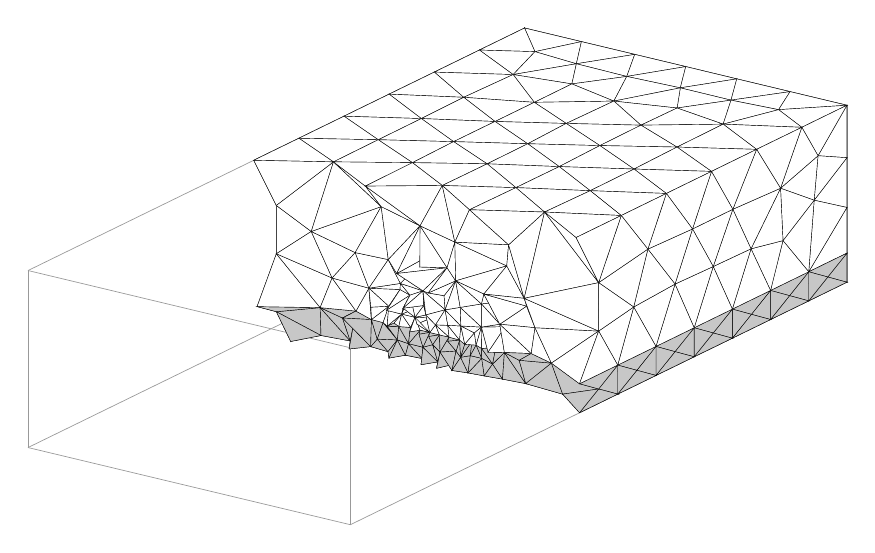
\begin{tikzpicture}
% generated by report/data/gen.py, do not edit
\draw[line width=0.25pt, black!40] (63.06mm,40.61mm) -- (63.06mm,63.08mm);
\draw[line width=0.25pt, black!40] (63.06mm,40.61mm) -- (104.00mm,30.80mm);
\draw[line width=0.25pt, black!40] (63.06mm,40.61mm) -- (0.00mm,9.80mm);
\draw[line width=0.25pt, black!40] (63.06mm,63.08mm) -- (104.00mm,53.27mm);
\draw[line width=0.25pt, black!40] (63.06mm,63.08mm) -- (0.00mm,32.28mm);
\draw[line width=0.25pt, black!40] (104.00mm,30.80mm) -- (104.00mm,53.27mm);
\draw[line width=0.25pt, black!40] (104.00mm,30.80mm) -- (40.94mm,0.00mm);
\draw[line width=0.25pt, black!40] (104.00mm,53.27mm) -- (40.94mm,22.47mm);
\draw[line width=0.25pt, black!40] (0.00mm,9.80mm) -- (0.00mm,32.28mm);
\draw[line width=0.25pt, black!40] (0.00mm,9.80mm) -- (40.94mm,0.00mm);
\draw[line width=0.25pt, black!40] (0.00mm,32.28mm) -- (40.94mm,22.47mm);
\draw[line width=0.25pt, black!40] (40.94mm,0.00mm) -- (40.94mm,22.47mm);
\filldraw[fill=black!22, draw=black, line width=0.15pt] (63.06mm,40.61mm) -- (63.06mm,44.29mm) -- (65.59mm,41.85mm) -- cycle;
\filldraw[fill=black!22, draw=black, line width=0.15pt] (63.06mm,40.61mm) -- (63.06mm,44.29mm) -- (60.64mm,41.27mm) -- cycle;
\filldraw[fill=black!22, draw=black, line width=0.15pt] (63.06mm,40.61mm) -- (68.16mm,39.39mm) -- (65.59mm,41.85mm) -- cycle;
\filldraw[fill=black!22, draw=black, line width=0.15pt] (63.06mm,40.61mm) -- (68.16mm,39.39mm) -- (64.28mm,38.87mm) -- cycle;
\filldraw[fill=black!22, draw=black, line width=0.15pt] (63.06mm,44.29mm) -- (68.07mm,43.09mm) -- (65.59mm,41.85mm) -- cycle;
\filldraw[fill=white, draw=black, line width=0.15pt] (63.06mm,44.29mm) -- (63.06mm,50.09mm) -- (67.13mm,47.25mm) -- cycle;
\filldraw[fill=black!22, draw=black, line width=0.15pt] (68.07mm,43.09mm) -- (68.16mm,39.39mm) -- (65.59mm,41.85mm) -- cycle;
\filldraw[fill=black!22, draw=black, line width=0.15pt] (63.06mm,40.61mm) -- (58.22mm,38.24mm) -- (60.64mm,41.27mm) -- cycle;
\filldraw[fill=black!22, draw=black, line width=0.15pt] (63.06mm,40.61mm) -- (58.22mm,38.24mm) -- (64.28mm,38.87mm) -- cycle;
\filldraw[fill=white, draw=black, line width=0.15pt] (63.06mm,44.29mm) -- (68.07mm,43.09mm) -- (67.13mm,47.25mm) -- cycle;
\filldraw[fill=white, draw=black, line width=0.15pt] (63.06mm,44.29mm) -- (58.22mm,41.93mm) -- (63.06mm,50.09mm) -- cycle;
\filldraw[fill=black!22, draw=black, line width=0.15pt] (63.06mm,44.29mm) -- (58.22mm,41.93mm) -- (60.64mm,41.27mm) -- cycle;
\filldraw[fill=black!22, draw=black, line width=0.15pt] (68.07mm,43.09mm) -- (68.16mm,39.39mm) -- (69.96mm,40.80mm) -- cycle;
\filldraw[fill=black!22, draw=black, line width=0.15pt] (68.16mm,39.39mm) -- (71.93mm,38.48mm) -- (69.96mm,40.80mm) -- cycle;
\filldraw[fill=black!22, draw=black, line width=0.15pt] (68.16mm,39.39mm) -- (68.23mm,38.04mm) -- (64.28mm,38.87mm) -- cycle;
\filldraw[fill=black!22, draw=black, line width=0.15pt] (68.16mm,39.39mm) -- (71.93mm,38.48mm) -- (68.23mm,38.04mm) -- cycle;
\filldraw[fill=black!22, draw=black, line width=0.15pt] (68.07mm,43.09mm) -- (71.66mm,42.23mm) -- (69.96mm,40.80mm) -- cycle;
\filldraw[fill=white, draw=black, line width=0.15pt] (63.06mm,50.09mm) -- (68.59mm,52.01mm) -- (67.13mm,47.25mm) -- cycle;
\filldraw[fill=white, draw=black, line width=0.15pt] (68.07mm,43.09mm) -- (70.42mm,45.06mm) -- (67.13mm,47.25mm) -- cycle;
\filldraw[fill=white, draw=black, line width=0.15pt] (63.06mm,50.09mm) -- (63.06mm,56.42mm) -- (68.59mm,52.01mm) -- cycle;
\filldraw[fill=black!22, draw=black, line width=0.15pt] (71.66mm,42.23mm) -- (71.93mm,38.48mm) -- (69.96mm,40.80mm) -- cycle;
\filldraw[fill=black!22, draw=black, line width=0.15pt] (58.22mm,38.24mm) -- (58.22mm,41.93mm) -- (60.64mm,41.27mm) -- cycle;
\filldraw[fill=white, draw=black, line width=0.15pt] (68.07mm,43.09mm) -- (71.66mm,42.23mm) -- (70.42mm,45.06mm) -- cycle;
\filldraw[fill=white, draw=black, line width=0.15pt] (63.06mm,50.09mm) -- (63.06mm,56.42mm) -- (58.91mm,51.01mm) -- cycle;
\filldraw[fill=black!22, draw=black, line width=0.15pt] (58.22mm,38.24mm) -- (64.58mm,37.40mm) -- (64.28mm,38.87mm) -- cycle;
\filldraw[fill=black!22, draw=black, line width=0.15pt] (71.66mm,42.23mm) -- (71.93mm,38.48mm) -- (73.50mm,39.84mm) -- cycle;
\filldraw[fill=black!22, draw=black, line width=0.15pt] (64.58mm,37.40mm) -- (68.23mm,38.04mm) -- (64.28mm,38.87mm) -- cycle;
\filldraw[fill=black!22, draw=black, line width=0.15pt] (71.93mm,38.48mm) -- (74.71mm,37.82mm) -- (73.50mm,39.84mm) -- cycle;
\filldraw[fill=white, draw=black, line width=0.15pt] (58.22mm,41.93mm) -- (63.06mm,50.09mm) -- (58.91mm,51.01mm) -- cycle;
\filldraw[fill=white, draw=black, line width=0.15pt] (70.42mm,45.06mm) -- (71.92mm,48.01mm) -- (67.13mm,47.25mm) -- cycle;
\filldraw[fill=black!22, draw=black, line width=0.15pt] (71.93mm,38.48mm) -- (71.95mm,37.20mm) -- (68.23mm,38.04mm) -- cycle;
\filldraw[fill=black!22, draw=black, line width=0.15pt] (71.93mm,38.48mm) -- (74.71mm,37.82mm) -- (71.95mm,37.20mm) -- cycle;
\filldraw[fill=white, draw=black, line width=0.15pt] (68.59mm,52.01mm) -- (71.92mm,48.01mm) -- (67.13mm,47.25mm) -- cycle;
\filldraw[fill=black!22, draw=black, line width=0.15pt] (71.66mm,42.23mm) -- (74.24mm,41.62mm) -- (73.50mm,39.84mm) -- cycle;
\filldraw[fill=white, draw=black, line width=0.15pt] (71.66mm,42.23mm) -- (73.56mm,44.41mm) -- (70.42mm,45.06mm) -- cycle;
\filldraw[fill=white, draw=black, line width=0.15pt] (63.06mm,63.08mm) -- (63.06mm,56.42mm) -- (67.39mm,57.68mm) -- cycle;
\filldraw[fill=white, draw=black, line width=0.15pt] (63.06mm,56.42mm) -- (68.59mm,52.01mm) -- (67.39mm,57.68mm) -- cycle;
\filldraw[fill=black!22, draw=black, line width=0.15pt] (74.71mm,37.82mm) -- (75.77mm,39.22mm) -- (73.50mm,39.84mm) -- cycle;
\filldraw[fill=black!22, draw=black, line width=0.15pt] (58.22mm,38.24mm) -- (58.22mm,41.93mm) -- (55.80mm,38.91mm) -- cycle;
\filldraw[fill=white, draw=black, line width=0.15pt] (71.66mm,42.23mm) -- (74.24mm,41.62mm) -- (73.56mm,44.41mm) -- cycle;
\filldraw[fill=black!22, draw=black, line width=0.15pt] (74.24mm,41.62mm) -- (75.77mm,39.22mm) -- (73.50mm,39.84mm) -- cycle;
\filldraw[fill=white, draw=black, line width=0.15pt] (63.06mm,63.08mm) -- (63.06mm,56.42mm) -- (59.40mm,56.66mm) -- cycle;
\filldraw[fill=white, draw=black, line width=0.15pt] (73.56mm,44.41mm) -- (70.42mm,45.06mm) -- (71.92mm,48.01mm) -- cycle;
\filldraw[fill=black!22, draw=black, line width=0.15pt] (74.71mm,37.82mm) -- (76.83mm,37.31mm) -- (75.77mm,39.22mm) -- cycle;
\filldraw[fill=black!22, draw=black, line width=0.15pt] (64.58mm,37.40mm) -- (68.67mm,36.73mm) -- (68.23mm,38.04mm) -- cycle;
\filldraw[fill=black!22, draw=black, line width=0.15pt] (74.71mm,37.82mm) -- (76.83mm,37.31mm) -- (74.75mm,37.02mm) -- cycle;
\filldraw[fill=black!22, draw=black, line width=0.15pt] (74.71mm,37.82mm) -- (71.95mm,37.20mm) -- (74.75mm,37.02mm) -- cycle;
\filldraw[fill=black!22, draw=black, line width=0.15pt] (71.95mm,37.20mm) -- (68.67mm,36.73mm) -- (68.23mm,38.04mm) -- cycle;
\filldraw[fill=white, draw=black, line width=0.15pt] (63.06mm,56.42mm) -- (58.91mm,51.01mm) -- (59.40mm,56.66mm) -- cycle;
\filldraw[fill=black!22, draw=black, line width=0.15pt] (74.24mm,41.62mm) -- (76.09mm,41.17mm) -- (75.77mm,39.22mm) -- cycle;
\filldraw[fill=white, draw=black, line width=0.15pt] (74.24mm,41.62mm) -- (73.56mm,44.41mm) -- (75.37mm,42.71mm) -- cycle;
\filldraw[fill=black!22, draw=black, line width=0.15pt] (76.83mm,37.31mm) -- (75.77mm,39.22mm) -- (77.45mm,38.46mm) -- cycle;
\filldraw[fill=black!22, draw=black, line width=0.15pt] (58.22mm,38.24mm) -- (61.45mm,35.95mm) -- (64.58mm,37.40mm) -- cycle;
\filldraw[fill=white, draw=black, line width=0.15pt] (74.24mm,41.62mm) -- (76.09mm,41.17mm) -- (75.37mm,42.71mm) -- cycle;
\filldraw[fill=black!22, draw=black, line width=0.15pt] (76.09mm,41.17mm) -- (75.77mm,39.22mm) -- (76.91mm,39.87mm) -- cycle;
\filldraw[fill=black!22, draw=black, line width=0.15pt] (75.77mm,39.22mm) -- (76.91mm,39.87mm) -- (77.45mm,38.46mm) -- cycle;
\filldraw[fill=black!22, draw=black, line width=0.15pt] (78.62mm,36.88mm) -- (76.83mm,37.31mm) -- (77.45mm,38.46mm) -- cycle;
\filldraw[fill=white, draw=black, line width=0.15pt] (68.59mm,52.01mm) -- (71.92mm,48.01mm) -- (74.14mm,50.30mm) -- cycle;
\filldraw[fill=white, draw=black, line width=0.15pt] (73.56mm,44.41mm) -- (71.92mm,48.01mm) -- (75.12mm,46.73mm) -- cycle;
\filldraw[fill=black!22, draw=black, line width=0.15pt] (58.22mm,38.24mm) -- (53.38mm,35.88mm) -- (55.80mm,38.91mm) -- cycle;
\filldraw[fill=black!22, draw=black, line width=0.15pt] (76.83mm,37.31mm) -- (76.55mm,36.56mm) -- (74.75mm,37.02mm) -- cycle;
\filldraw[fill=white, draw=black, line width=0.15pt] (68.59mm,52.01mm) -- (72.48mm,55.48mm) -- (67.39mm,57.68mm) -- cycle;
\filldraw[fill=white, draw=black, line width=0.15pt] (73.56mm,44.41mm) -- (75.37mm,42.71mm) -- (76.17mm,44.24mm) -- cycle;
\filldraw[fill=black!22, draw=black, line width=0.15pt] (78.62mm,36.88mm) -- (76.83mm,37.31mm) -- (76.55mm,36.56mm) -- cycle;
\filldraw[fill=black!22, draw=black, line width=0.15pt] (77.95mm,39.14mm) -- (76.91mm,39.87mm) -- (77.45mm,38.46mm) -- cycle;
\filldraw[fill=white, draw=black, line width=0.15pt] (63.06mm,63.08mm) -- (70.28mm,61.35mm) -- (67.39mm,57.68mm) -- cycle;
\filldraw[fill=black!22, draw=black, line width=0.15pt] (76.09mm,41.17mm) -- (77.42mm,40.85mm) -- (76.91mm,39.87mm) -- cycle;
\filldraw[fill=white, draw=black, line width=0.15pt] (76.09mm,41.17mm) -- (76.84mm,42.41mm) -- (75.37mm,42.71mm) -- cycle;
\filldraw[fill=black!22, draw=black, line width=0.15pt] (78.62mm,36.88mm) -- (78.62mm,38.33mm) -- (77.45mm,38.46mm) -- cycle;
\filldraw[fill=black!22, draw=black, line width=0.15pt] (71.95mm,37.20mm) -- (74.75mm,37.02mm) -- (73.96mm,36.27mm) -- cycle;
\filldraw[fill=black!22, draw=black, line width=0.15pt] (78.62mm,38.33mm) -- (77.95mm,39.14mm) -- (77.45mm,38.46mm) -- cycle;
\filldraw[fill=black!22, draw=black, line width=0.15pt] (77.95mm,39.14mm) -- (76.91mm,39.87mm) -- (77.96mm,40.07mm) -- cycle;
\filldraw[fill=white, draw=black, line width=0.15pt] (73.56mm,44.41mm) -- (76.17mm,44.24mm) -- (75.12mm,46.73mm) -- cycle;
\filldraw[fill=white, draw=black, line width=0.15pt] (76.09mm,41.17mm) -- (77.42mm,40.85mm) -- (76.84mm,42.41mm) -- cycle;
\filldraw[fill=black!22, draw=black, line width=0.15pt] (77.42mm,40.85mm) -- (76.91mm,39.87mm) -- (77.96mm,40.07mm) -- cycle;
\filldraw[fill=white, draw=black, line width=0.15pt] (76.84mm,42.41mm) -- (75.37mm,42.71mm) -- (76.17mm,44.24mm) -- cycle;
\filldraw[fill=white, draw=black, line width=0.15pt] (58.22mm,41.93mm) -- (58.91mm,51.01mm) -- (54.96mm,45.89mm) -- cycle;
\filldraw[fill=black!22, draw=black, line width=0.15pt] (78.62mm,36.88mm) -- (78.62mm,38.33mm) -- (79.61mm,37.48mm) -- cycle;
\filldraw[fill=black!22, draw=black, line width=0.15pt] (58.22mm,38.24mm) -- (53.38mm,35.88mm) -- (61.45mm,35.95mm) -- cycle;
\filldraw[fill=white, draw=black, line width=0.15pt] (71.92mm,48.01mm) -- (75.12mm,46.73mm) -- (74.14mm,50.30mm) -- cycle;
\filldraw[fill=white, draw=black, line width=0.15pt] (68.59mm,52.01mm) -- (72.48mm,55.48mm) -- (74.14mm,50.30mm) -- cycle;
\filldraw[fill=black!22, draw=black, line width=0.15pt] (78.62mm,38.33mm) -- (78.62mm,39.47mm) -- (77.95mm,39.14mm) -- cycle;
\filldraw[fill=black!22, draw=black, line width=0.15pt] (71.95mm,37.20mm) -- (71.52mm,36.06mm) -- (68.67mm,36.73mm) -- cycle;
\filldraw[fill=black!22, draw=black, line width=0.15pt] (58.22mm,41.93mm) -- (53.39mm,39.57mm) -- (55.80mm,38.91mm) -- cycle;
\filldraw[fill=black!22, draw=black, line width=0.15pt] (78.62mm,39.47mm) -- (77.95mm,39.14mm) -- (77.96mm,40.07mm) -- cycle;
\filldraw[fill=black!22, draw=black, line width=0.15pt] (76.55mm,36.56mm) -- (74.75mm,37.02mm) -- (73.96mm,36.27mm) -- cycle;
\filldraw[fill=black!22, draw=black, line width=0.15pt] (78.62mm,36.88mm) -- (80.57mm,36.41mm) -- (79.61mm,37.48mm) -- cycle;
\filldraw[fill=black!22, draw=black, line width=0.15pt] (78.62mm,40.57mm) -- (77.42mm,40.85mm) -- (77.96mm,40.07mm) -- cycle;
\filldraw[fill=white, draw=black, line width=0.15pt] (77.42mm,40.85mm) -- (76.84mm,42.41mm) -- (78.02mm,41.92mm) -- cycle;
\filldraw[fill=black!22, draw=black, line width=0.15pt] (64.58mm,37.40mm) -- (66.69mm,35.55mm) -- (68.67mm,36.73mm) -- cycle;
\filldraw[fill=black!22, draw=black, line width=0.15pt] (78.62mm,38.33mm) -- (78.62mm,39.47mm) -- (79.46mm,38.69mm) -- cycle;
\filldraw[fill=black!22, draw=black, line width=0.15pt] (78.62mm,38.33mm) -- (79.46mm,38.69mm) -- (79.61mm,37.48mm) -- cycle;
\filldraw[fill=black!22, draw=black, line width=0.15pt] (78.62mm,40.57mm) -- (78.62mm,39.47mm) -- (77.96mm,40.07mm) -- cycle;
\filldraw[fill=black!22, draw=black, line width=0.15pt] (78.62mm,36.88mm) -- (76.55mm,36.56mm) -- (78.33mm,36.10mm) -- cycle;
\filldraw[fill=black!22, draw=black, line width=0.15pt] (71.95mm,37.20mm) -- (71.52mm,36.06mm) -- (73.96mm,36.27mm) -- cycle;
\filldraw[fill=white, draw=black, line width=0.15pt] (78.62mm,40.57mm) -- (77.42mm,40.85mm) -- (78.02mm,41.92mm) -- cycle;
\filldraw[fill=black!22, draw=black, line width=0.15pt] (78.62mm,36.88mm) -- (80.57mm,36.41mm) -- (78.33mm,36.10mm) -- cycle;
\filldraw[fill=white, draw=black, line width=0.15pt] (76.84mm,42.41mm) -- (76.17mm,44.24mm) -- (78.07mm,43.27mm) -- cycle;
\filldraw[fill=black!22, draw=black, line width=0.15pt] (78.62mm,39.47mm) -- (79.46mm,38.69mm) -- (79.39mm,39.63mm) -- cycle;
\filldraw[fill=black!22, draw=black, line width=0.15pt] (78.62mm,40.57mm) -- (78.62mm,39.47mm) -- (79.39mm,39.63mm) -- cycle;
\filldraw[fill=white, draw=black, line width=0.15pt] (76.84mm,42.41mm) -- (78.07mm,43.27mm) -- (78.02mm,41.92mm) -- cycle;
\filldraw[fill=white, draw=black, line width=0.15pt] (70.28mm,61.35mm) -- (72.48mm,55.48mm) -- (67.39mm,57.68mm) -- cycle;
\filldraw[fill=white, draw=black, line width=0.15pt] (76.17mm,44.24mm) -- (77.46mm,45.50mm) -- (75.12mm,46.73mm) -- cycle;
\filldraw[fill=black!22, draw=black, line width=0.15pt] (80.57mm,36.41mm) -- (79.61mm,37.48mm) -- (81.04mm,37.59mm) -- cycle;
\filldraw[fill=black!22, draw=black, line width=0.15pt] (79.46mm,38.69mm) -- (79.61mm,37.48mm) -- (81.04mm,37.59mm) -- cycle;
\filldraw[fill=white, draw=black, line width=0.15pt] (63.06mm,63.08mm) -- (57.33mm,60.28mm) -- (59.40mm,56.66mm) -- cycle;
\filldraw[fill=black!22, draw=black, line width=0.15pt] (61.45mm,35.95mm) -- (64.58mm,37.40mm) -- (66.69mm,35.55mm) -- cycle;
\filldraw[fill=white, draw=black, line width=0.15pt] (78.62mm,40.57mm) -- (79.15mm,41.68mm) -- (78.02mm,41.92mm) -- cycle;
\filldraw[fill=black!22, draw=black, line width=0.15pt] (79.46mm,38.69mm) -- (80.40mm,39.17mm) -- (79.39mm,39.63mm) -- cycle;
\filldraw[fill=white, draw=black, line width=0.15pt] (76.17mm,44.24mm) -- (78.07mm,43.27mm) -- (77.46mm,45.50mm) -- cycle;
\filldraw[fill=black!22, draw=black, line width=0.15pt] (78.62mm,40.57mm) -- (79.85mm,40.27mm) -- (79.39mm,39.63mm) -- cycle;
\filldraw[fill=white, draw=black, line width=0.15pt] (78.07mm,43.27mm) -- (79.15mm,41.68mm) -- (78.02mm,41.92mm) -- cycle;
\filldraw[fill=black!22, draw=black, line width=0.15pt] (79.46mm,38.69mm) -- (80.40mm,39.17mm) -- (81.04mm,37.59mm) -- cycle;
\filldraw[fill=black!22, draw=black, line width=0.15pt] (76.55mm,36.56mm) -- (75.90mm,35.80mm) -- (73.96mm,36.27mm) -- cycle;
\filldraw[fill=white, draw=black, line width=0.15pt] (77.17mm,48.29mm) -- (75.12mm,46.73mm) -- (74.14mm,50.30mm) -- cycle;
\filldraw[fill=white, draw=black, line width=0.15pt] (78.62mm,40.57mm) -- (79.85mm,40.27mm) -- (79.15mm,41.68mm) -- cycle;
\filldraw[fill=white, draw=black, line width=0.15pt] (58.22mm,41.93mm) -- (53.39mm,39.57mm) -- (54.96mm,45.89mm) -- cycle;
\filldraw[fill=black!22, draw=black, line width=0.15pt] (79.85mm,40.27mm) -- (80.40mm,39.17mm) -- (79.39mm,39.63mm) -- cycle;
\filldraw[fill=black!22, draw=black, line width=0.15pt] (82.52mm,35.95mm) -- (80.57mm,36.41mm) -- (81.04mm,37.59mm) -- cycle;
\filldraw[fill=black!22, draw=black, line width=0.15pt] (76.55mm,36.56mm) -- (78.33mm,36.10mm) -- (75.90mm,35.80mm) -- cycle;
\filldraw[fill=black!22, draw=black, line width=0.15pt] (71.52mm,36.06mm) -- (68.67mm,36.73mm) -- (69.44mm,35.57mm) -- cycle;
\filldraw[fill=white, draw=black, line width=0.15pt] (77.17mm,48.29mm) -- (77.46mm,45.50mm) -- (75.12mm,46.73mm) -- cycle;
\filldraw[fill=white, draw=black, line width=0.15pt] (63.06mm,63.08mm) -- (70.28mm,61.35mm) -- (64.38mm,60.08mm) -- cycle;
\filldraw[fill=black!22, draw=black, line width=0.15pt] (80.57mm,36.41mm) -- (80.36mm,35.63mm) -- (78.33mm,36.10mm) -- cycle;
\filldraw[fill=black!22, draw=black, line width=0.15pt] (53.38mm,35.88mm) -- (53.39mm,39.57mm) -- (55.80mm,38.91mm) -- cycle;
\filldraw[fill=white, draw=black, line width=0.15pt] (78.07mm,43.27mm) -- (79.15mm,41.68mm) -- (79.73mm,42.85mm) -- cycle;
\filldraw[fill=black!22, draw=black, line width=0.15pt] (81.69mm,38.61mm) -- (80.40mm,39.17mm) -- (81.04mm,37.59mm) -- cycle;
\filldraw[fill=white, draw=black, line width=0.15pt] (78.07mm,43.27mm) -- (77.46mm,45.50mm) -- (78.97mm,44.43mm) -- cycle;
\filldraw[fill=black!22, draw=black, line width=0.15pt] (79.85mm,40.27mm) -- (81.07mm,39.98mm) -- (80.40mm,39.17mm) -- cycle;
\filldraw[fill=black!22, draw=black, line width=0.15pt] (82.52mm,35.95mm) -- (80.57mm,36.41mm) -- (80.36mm,35.63mm) -- cycle;
\filldraw[fill=white, draw=black, line width=0.15pt] (79.85mm,40.27mm) -- (80.48mm,41.35mm) -- (79.15mm,41.68mm) -- cycle;
\filldraw[fill=black!22, draw=black, line width=0.15pt] (82.52mm,35.95mm) -- (81.04mm,37.59mm) -- (82.34mm,37.51mm) -- cycle;
\filldraw[fill=black!22, draw=black, line width=0.15pt] (66.69mm,35.55mm) -- (68.67mm,36.73mm) -- (69.44mm,35.57mm) -- cycle;
\filldraw[fill=black!22, draw=black, line width=0.15pt] (73.66mm,35.46mm) -- (71.52mm,36.06mm) -- (73.96mm,36.27mm) -- cycle;
\filldraw[fill=white, draw=black, line width=0.15pt] (78.07mm,43.27mm) -- (79.73mm,42.85mm) -- (78.97mm,44.43mm) -- cycle;
\filldraw[fill=white, draw=black, line width=0.15pt] (58.91mm,51.01mm) -- (54.64mm,52.53mm) -- (59.40mm,56.66mm) -- cycle;
\filldraw[fill=black!22, draw=black, line width=0.15pt] (81.69mm,38.61mm) -- (81.04mm,37.59mm) -- (82.34mm,37.51mm) -- cycle;
\filldraw[fill=black!22, draw=black, line width=0.15pt] (81.07mm,39.98mm) -- (81.69mm,38.61mm) -- (80.40mm,39.17mm) -- cycle;
\filldraw[fill=white, draw=black, line width=0.15pt] (79.85mm,40.27mm) -- (81.07mm,39.98mm) -- (80.48mm,41.35mm) -- cycle;
\filldraw[fill=white, draw=black, line width=0.15pt] (80.48mm,41.35mm) -- (79.15mm,41.68mm) -- (79.73mm,42.85mm) -- cycle;
\filldraw[fill=white, draw=black, line width=0.15pt] (72.48mm,55.48mm) -- (74.14mm,50.30mm) -- (76.84mm,52.76mm) -- cycle;
\filldraw[fill=black!22, draw=black, line width=0.15pt] (73.66mm,35.46mm) -- (75.90mm,35.80mm) -- (73.96mm,36.27mm) -- cycle;
\filldraw[fill=white, draw=black, line width=0.15pt] (77.17mm,48.29mm) -- (74.14mm,50.30mm) -- (76.84mm,52.76mm) -- cycle;
\filldraw[fill=white, draw=black, line width=0.15pt] (77.46mm,45.50mm) -- (79.15mm,46.25mm) -- (78.97mm,44.43mm) -- cycle;
\filldraw[fill=white, draw=black, line width=0.15pt] (77.17mm,48.29mm) -- (77.46mm,45.50mm) -- (79.15mm,46.25mm) -- cycle;
\filldraw[fill=black!22, draw=black, line width=0.15pt] (82.52mm,35.95mm) -- (83.53mm,37.00mm) -- (82.34mm,37.51mm) -- cycle;
\filldraw[fill=black!22, draw=black, line width=0.15pt] (78.00mm,35.32mm) -- (78.33mm,36.10mm) -- (75.90mm,35.80mm) -- cycle;
\filldraw[fill=black!22, draw=black, line width=0.15pt] (81.07mm,39.98mm) -- (82.30mm,39.69mm) -- (81.69mm,38.61mm) -- cycle;
\filldraw[fill=black!22, draw=black, line width=0.15pt] (81.69mm,38.61mm) -- (82.89mm,38.38mm) -- (82.34mm,37.51mm) -- cycle;
\filldraw[fill=white, draw=black, line width=0.15pt] (63.06mm,63.08mm) -- (57.33mm,60.28mm) -- (64.38mm,60.08mm) -- cycle;
\filldraw[fill=white, draw=black, line width=0.15pt] (81.07mm,39.98mm) -- (80.48mm,41.35mm) -- (81.78mm,41.03mm) -- cycle;
\filldraw[fill=black!22, draw=black, line width=0.15pt] (78.00mm,35.32mm) -- (80.36mm,35.63mm) -- (78.33mm,36.10mm) -- cycle;
\filldraw[fill=white, draw=black, line width=0.15pt] (80.48mm,41.35mm) -- (79.73mm,42.85mm) -- (81.23mm,42.53mm) -- cycle;
\filldraw[fill=white, draw=black, line width=0.15pt] (79.73mm,42.85mm) -- (80.42mm,44.30mm) -- (78.97mm,44.43mm) -- cycle;
\filldraw[fill=black!22, draw=black, line width=0.15pt] (84.54mm,35.46mm) -- (82.52mm,35.95mm) -- (83.53mm,37.00mm) -- cycle;
\filldraw[fill=black!22, draw=black, line width=0.15pt] (82.30mm,39.69mm) -- (81.69mm,38.61mm) -- (82.89mm,38.38mm) -- cycle;
\filldraw[fill=black!22, draw=black, line width=0.15pt] (83.53mm,37.00mm) -- (82.89mm,38.38mm) -- (82.34mm,37.51mm) -- cycle;
\filldraw[fill=white, draw=black, line width=0.15pt] (81.07mm,39.98mm) -- (82.30mm,39.69mm) -- (81.78mm,41.03mm) -- cycle;
\filldraw[fill=white, draw=black, line width=0.15pt] (58.91mm,51.01mm) -- (54.96mm,45.89mm) -- (54.64mm,52.53mm) -- cycle;
\filldraw[fill=black!22, draw=black, line width=0.15pt] (82.52mm,35.95mm) -- (82.35mm,35.15mm) -- (80.36mm,35.63mm) -- cycle;
\filldraw[fill=black!22, draw=black, line width=0.15pt] (71.48mm,35.09mm) -- (71.52mm,36.06mm) -- (69.44mm,35.57mm) -- cycle;
\filldraw[fill=white, draw=black, line width=0.15pt] (80.42mm,44.30mm) -- (79.15mm,46.25mm) -- (78.97mm,44.43mm) -- cycle;
\filldraw[fill=white, draw=black, line width=0.15pt] (80.48mm,41.35mm) -- (81.23mm,42.53mm) -- (81.78mm,41.03mm) -- cycle;
\filldraw[fill=white, draw=black, line width=0.15pt] (79.73mm,42.85mm) -- (81.23mm,42.53mm) -- (80.42mm,44.30mm) -- cycle;
\filldraw[fill=black!22, draw=black, line width=0.15pt] (73.66mm,35.46mm) -- (71.48mm,35.09mm) -- (71.52mm,36.06mm) -- cycle;
\filldraw[fill=black!22, draw=black, line width=0.15pt] (84.54mm,35.46mm) -- (82.52mm,35.95mm) -- (82.35mm,35.15mm) -- cycle;
\filldraw[fill=black!22, draw=black, line width=0.15pt] (83.53mm,37.00mm) -- (82.89mm,38.38mm) -- (84.14mm,38.06mm) -- cycle;
\filldraw[fill=white, draw=black, line width=0.15pt] (70.28mm,61.35mm) -- (77.05mm,59.73mm) -- (72.48mm,55.48mm) -- cycle;
\filldraw[fill=black!22, draw=black, line width=0.15pt] (82.30mm,39.69mm) -- (83.53mm,39.39mm) -- (82.89mm,38.38mm) -- cycle;
\filldraw[fill=black!22, draw=black, line width=0.15pt] (75.69mm,34.99mm) -- (73.66mm,35.46mm) -- (75.90mm,35.80mm) -- cycle;
\filldraw[fill=white, draw=black, line width=0.15pt] (82.30mm,39.69mm) -- (81.78mm,41.03mm) -- (82.92mm,40.50mm) -- cycle;
\filldraw[fill=black!22, draw=black, line width=0.15pt] (84.54mm,35.46mm) -- (83.53mm,37.00mm) -- (84.72mm,36.93mm) -- cycle;
\filldraw[fill=white, draw=black, line width=0.15pt] (77.17mm,48.29mm) -- (79.15mm,46.25mm) -- (79.84mm,48.98mm) -- cycle;
\filldraw[fill=black!22, draw=black, line width=0.15pt] (53.38mm,35.88mm) -- (61.45mm,35.95mm) -- (59.81mm,34.34mm) -- cycle;
\filldraw[fill=black!22, draw=black, line width=0.15pt] (75.69mm,34.99mm) -- (78.00mm,35.32mm) -- (75.90mm,35.80mm) -- cycle;
\filldraw[fill=black!22, draw=black, line width=0.15pt] (61.45mm,35.95mm) -- (66.69mm,35.55mm) -- (64.58mm,34.49mm) -- cycle;
\filldraw[fill=black!22, draw=black, line width=0.15pt] (83.53mm,37.00mm) -- (84.14mm,38.06mm) -- (84.72mm,36.93mm) -- cycle;
\filldraw[fill=white, draw=black, line width=0.15pt] (77.17mm,48.29mm) -- (79.84mm,48.98mm) -- (76.84mm,52.76mm) -- cycle;
\filldraw[fill=black!22, draw=black, line width=0.15pt] (83.53mm,39.39mm) -- (82.89mm,38.38mm) -- (84.14mm,38.06mm) -- cycle;
\filldraw[fill=white, draw=black, line width=0.15pt] (82.30mm,39.69mm) -- (83.53mm,39.39mm) -- (82.92mm,40.50mm) -- cycle;
\filldraw[fill=white, draw=black, line width=0.15pt] (81.23mm,42.53mm) -- (82.93mm,41.94mm) -- (81.78mm,41.03mm) -- cycle;
\filldraw[fill=white, draw=black, line width=0.15pt] (80.42mm,44.30mm) -- (81.00mm,46.03mm) -- (79.15mm,46.25mm) -- cycle;
\filldraw[fill=black!22, draw=black, line width=0.15pt] (66.69mm,35.55mm) -- (69.25mm,34.79mm) -- (69.44mm,35.57mm) -- cycle;
\filldraw[fill=white, draw=black, line width=0.15pt] (81.23mm,42.53mm) -- (80.42mm,44.30mm) -- (82.17mm,44.11mm) -- cycle;
\filldraw[fill=black!22, draw=black, line width=0.15pt] (78.00mm,35.32mm) -- (80.36mm,35.63mm) -- (80.03mm,34.84mm) -- cycle;
\filldraw[fill=white, draw=black, line width=0.15pt] (82.93mm,41.94mm) -- (81.78mm,41.03mm) -- (82.92mm,40.50mm) -- cycle;
\filldraw[fill=black!22, draw=black, line width=0.15pt] (53.38mm,35.88mm) -- (53.39mm,39.57mm) -- (50.97mm,36.54mm) -- cycle;
\filldraw[fill=white, draw=black, line width=0.15pt] (57.33mm,60.28mm) -- (54.64mm,52.53mm) -- (59.40mm,56.66mm) -- cycle;
\filldraw[fill=white, draw=black, line width=0.15pt] (77.05mm,59.73mm) -- (72.48mm,55.48mm) -- (76.84mm,52.76mm) -- cycle;
\filldraw[fill=black!22, draw=black, line width=0.15pt] (84.54mm,35.46mm) -- (86.02mm,36.39mm) -- (84.72mm,36.93mm) -- cycle;
\filldraw[fill=black!22, draw=black, line width=0.15pt] (82.35mm,35.15mm) -- (80.36mm,35.63mm) -- (80.03mm,34.84mm) -- cycle;
\filldraw[fill=white, draw=black, line width=0.15pt] (81.00mm,46.03mm) -- (79.15mm,46.25mm) -- (79.84mm,48.98mm) -- cycle;
\filldraw[fill=black!22, draw=black, line width=0.15pt] (71.48mm,35.09mm) -- (69.25mm,34.79mm) -- (69.44mm,35.57mm) -- cycle;
\filldraw[fill=white, draw=black, line width=0.15pt] (81.23mm,42.53mm) -- (82.17mm,44.11mm) -- (82.93mm,41.94mm) -- cycle;
\filldraw[fill=black!22, draw=black, line width=0.15pt] (86.49mm,35.00mm) -- (84.54mm,35.46mm) -- (86.02mm,36.39mm) -- cycle;
\filldraw[fill=white, draw=black, line width=0.15pt] (80.42mm,44.30mm) -- (82.17mm,44.11mm) -- (81.00mm,46.03mm) -- cycle;
\filldraw[fill=white, draw=black, line width=0.15pt] (83.53mm,39.39mm) -- (84.03mm,40.46mm) -- (82.92mm,40.50mm) -- cycle;
\filldraw[fill=black!22, draw=black, line width=0.15pt] (85.37mm,37.73mm) -- (84.14mm,38.06mm) -- (84.72mm,36.93mm) -- cycle;
\filldraw[fill=black!22, draw=black, line width=0.15pt] (83.53mm,39.39mm) -- (84.76mm,39.10mm) -- (84.14mm,38.06mm) -- cycle;
\filldraw[fill=black!22, draw=black, line width=0.15pt] (84.54mm,35.46mm) -- (82.35mm,35.15mm) -- (84.37mm,34.70mm) -- cycle;
\filldraw[fill=white, draw=black, line width=0.15pt] (84.03mm,40.46mm) -- (82.93mm,41.94mm) -- (82.92mm,40.50mm) -- cycle;
\filldraw[fill=black!22, draw=black, line width=0.15pt] (73.50mm,34.63mm) -- (73.66mm,35.46mm) -- (71.48mm,35.09mm) -- cycle;
\filldraw[fill=black!22, draw=black, line width=0.15pt] (86.49mm,35.00mm) -- (84.54mm,35.46mm) -- (84.37mm,34.70mm) -- cycle;
\filldraw[fill=black!22, draw=black, line width=0.15pt] (85.37mm,37.73mm) -- (86.02mm,36.39mm) -- (84.72mm,36.93mm) -- cycle;
\filldraw[fill=black!22, draw=black, line width=0.15pt] (84.76mm,39.10mm) -- (85.37mm,37.73mm) -- (84.14mm,38.06mm) -- cycle;
\filldraw[fill=white, draw=black, line width=0.15pt] (83.53mm,39.39mm) -- (84.76mm,39.10mm) -- (84.03mm,40.46mm) -- cycle;
\filldraw[fill=black!22, draw=black, line width=0.15pt] (75.69mm,34.99mm) -- (73.50mm,34.63mm) -- (73.66mm,35.46mm) -- cycle;
\filldraw[fill=black!22, draw=black, line width=0.15pt] (77.76mm,34.51mm) -- (75.69mm,34.99mm) -- (78.00mm,35.32mm) -- cycle;
\filldraw[fill=black!22, draw=black, line width=0.15pt] (61.45mm,35.95mm) -- (64.58mm,34.49mm) -- (59.81mm,34.34mm) -- cycle;
\filldraw[fill=black!22, draw=black, line width=0.15pt] (66.69mm,35.55mm) -- (69.25mm,34.79mm) -- (67.29mm,34.37mm) -- cycle;
\filldraw[fill=black!22, draw=black, line width=0.15pt] (77.76mm,34.51mm) -- (78.00mm,35.32mm) -- (80.03mm,34.84mm) -- cycle;
\filldraw[fill=white, draw=black, line width=0.15pt] (84.03mm,40.46mm) -- (82.93mm,41.94mm) -- (84.64mm,41.68mm) -- cycle;
\filldraw[fill=black!22, draw=black, line width=0.15pt] (86.49mm,35.00mm) -- (87.47mm,35.59mm) -- (86.02mm,36.39mm) -- cycle;
\filldraw[fill=white, draw=black, line width=0.15pt] (82.17mm,44.11mm) -- (82.93mm,41.94mm) -- (84.07mm,43.52mm) -- cycle;
\filldraw[fill=black!22, draw=black, line width=0.15pt] (84.76mm,39.10mm) -- (85.99mm,38.80mm) -- (85.37mm,37.73mm) -- cycle;
\filldraw[fill=white, draw=black, line width=0.15pt] (84.76mm,39.10mm) -- (84.03mm,40.46mm) -- (85.36mm,40.16mm) -- cycle;
\filldraw[fill=black!22, draw=black, line width=0.15pt] (85.37mm,37.73mm) -- (86.64mm,37.66mm) -- (86.02mm,36.39mm) -- cycle;
\filldraw[fill=black!22, draw=black, line width=0.15pt] (66.69mm,35.55mm) -- (64.58mm,34.49mm) -- (67.29mm,34.37mm) -- cycle;
\filldraw[fill=white, draw=black, line width=0.15pt] (80.34mm,53.80mm) -- (79.84mm,48.98mm) -- (76.84mm,52.76mm) -- cycle;
\filldraw[fill=black!22, draw=black, line width=0.15pt] (82.35mm,35.15mm) -- (80.03mm,34.84mm) -- (82.04mm,34.38mm) -- cycle;
\filldraw[fill=white, draw=black, line width=0.15pt] (83.41mm,46.53mm) -- (82.17mm,44.11mm) -- (81.00mm,46.03mm) -- cycle;
\filldraw[fill=white, draw=black, line width=0.15pt] (83.41mm,46.53mm) -- (81.00mm,46.03mm) -- (79.84mm,48.98mm) -- cycle;
\filldraw[fill=black!22, draw=black, line width=0.15pt] (82.35mm,35.15mm) -- (84.37mm,34.70mm) -- (82.04mm,34.38mm) -- cycle;
\filldraw[fill=white, draw=black, line width=0.15pt] (82.93mm,41.94mm) -- (84.07mm,43.52mm) -- (84.64mm,41.68mm) -- cycle;
\filldraw[fill=black!22, draw=black, line width=0.15pt] (88.44mm,34.53mm) -- (86.49mm,35.00mm) -- (87.47mm,35.59mm) -- cycle;
\filldraw[fill=white, draw=black, line width=0.15pt] (84.03mm,40.46mm) -- (85.36mm,40.16mm) -- (84.64mm,41.68mm) -- cycle;
\filldraw[fill=white, draw=black, line width=0.15pt] (84.76mm,39.10mm) -- (85.99mm,38.80mm) -- (85.36mm,40.16mm) -- cycle;
\filldraw[fill=black!22, draw=black, line width=0.15pt] (85.99mm,38.80mm) -- (85.37mm,37.73mm) -- (86.64mm,37.66mm) -- cycle;
\filldraw[fill=white, draw=black, line width=0.15pt] (53.39mm,39.57mm) -- (50.92mm,44.86mm) -- (54.96mm,45.89mm) -- cycle;
\filldraw[fill=black!22, draw=black, line width=0.15pt] (71.48mm,35.09mm) -- (71.39mm,34.25mm) -- (69.25mm,34.79mm) -- cycle;
\filldraw[fill=black!22, draw=black, line width=0.15pt] (87.46mm,36.72mm) -- (87.47mm,35.59mm) -- (86.02mm,36.39mm) -- cycle;
\filldraw[fill=black!22, draw=black, line width=0.15pt] (87.46mm,36.72mm) -- (86.64mm,37.66mm) -- (86.02mm,36.39mm) -- cycle;
\filldraw[fill=black!22, draw=black, line width=0.15pt] (73.50mm,34.63mm) -- (71.48mm,35.09mm) -- (71.39mm,34.25mm) -- cycle;
\filldraw[fill=black!22, draw=black, line width=0.15pt] (86.49mm,35.00mm) -- (86.41mm,34.25mm) -- (84.37mm,34.70mm) -- cycle;
\filldraw[fill=black!22, draw=black, line width=0.15pt] (53.38mm,35.88mm) -- (48.55mm,33.52mm) -- (50.97mm,36.54mm) -- cycle;
\filldraw[fill=white, draw=black, line width=0.15pt] (83.41mm,46.53mm) -- (82.17mm,44.11mm) -- (84.07mm,43.52mm) -- cycle;
\filldraw[fill=black!22, draw=black, line width=0.15pt] (75.53mm,34.16mm) -- (75.69mm,34.99mm) -- (73.50mm,34.63mm) -- cycle;
\filldraw[fill=black!22, draw=black, line width=0.15pt] (88.44mm,34.53mm) -- (86.49mm,35.00mm) -- (86.41mm,34.25mm) -- cycle;
\filldraw[fill=white, draw=black, line width=0.15pt] (77.05mm,59.73mm) -- (80.34mm,53.80mm) -- (76.84mm,52.76mm) -- cycle;
\filldraw[fill=black!22, draw=black, line width=0.15pt] (53.38mm,35.88mm) -- (55.57mm,33.48mm) -- (59.81mm,34.34mm) -- cycle;
\filldraw[fill=black!22, draw=black, line width=0.15pt] (77.76mm,34.51mm) -- (75.53mm,34.16mm) -- (75.69mm,34.99mm) -- cycle;
\filldraw[fill=white, draw=black, line width=0.15pt] (70.28mm,61.35mm) -- (69.64mm,58.54mm) -- (64.38mm,60.08mm) -- cycle;
\filldraw[fill=white, draw=black, line width=0.15pt] (85.99mm,38.80mm) -- (86.61mm,39.83mm) -- (85.36mm,40.16mm) -- cycle;
\filldraw[fill=black!22, draw=black, line width=0.15pt] (85.99mm,38.80mm) -- (87.22mm,38.51mm) -- (86.64mm,37.66mm) -- cycle;
\filldraw[fill=white, draw=black, line width=0.15pt] (85.36mm,40.16mm) -- (86.06mm,41.21mm) -- (84.64mm,41.68mm) -- cycle;
\filldraw[fill=black!22, draw=black, line width=0.15pt] (88.44mm,34.53mm) -- (88.44mm,35.97mm) -- (87.47mm,35.59mm) -- cycle;
\filldraw[fill=black!22, draw=black, line width=0.15pt] (88.44mm,35.97mm) -- (87.46mm,36.72mm) -- (87.47mm,35.59mm) -- cycle;
\filldraw[fill=black!22, draw=black, line width=0.15pt] (87.46mm,36.72mm) -- (86.64mm,37.66mm) -- (87.64mm,37.64mm) -- cycle;
\filldraw[fill=black!22, draw=black, line width=0.15pt] (79.77mm,34.05mm) -- (77.76mm,34.51mm) -- (80.03mm,34.84mm) -- cycle;
\filldraw[fill=white, draw=black, line width=0.15pt] (84.07mm,43.52mm) -- (84.64mm,41.68mm) -- (85.49mm,42.65mm) -- cycle;
\filldraw[fill=white, draw=black, line width=0.15pt] (85.99mm,38.80mm) -- (87.22mm,38.51mm) -- (86.61mm,39.83mm) -- cycle;
\filldraw[fill=white, draw=black, line width=0.15pt] (70.28mm,61.35mm) -- (77.05mm,59.73mm) -- (69.64mm,58.54mm) -- cycle;
\filldraw[fill=black!22, draw=black, line width=0.15pt] (87.22mm,38.51mm) -- (86.64mm,37.66mm) -- (87.64mm,37.64mm) -- cycle;
\filldraw[fill=black!22, draw=black, line width=0.15pt] (79.77mm,34.05mm) -- (80.03mm,34.84mm) -- (82.04mm,34.38mm) -- cycle;
\filldraw[fill=white, draw=black, line width=0.15pt] (86.61mm,39.83mm) -- (85.36mm,40.16mm) -- (86.06mm,41.21mm) -- cycle;
\filldraw[fill=white, draw=black, line width=0.15pt] (86.06mm,41.21mm) -- (84.64mm,41.68mm) -- (85.49mm,42.65mm) -- cycle;
\filldraw[fill=white, draw=black, line width=0.15pt] (50.92mm,44.86mm) -- (54.96mm,45.89mm) -- (54.64mm,52.53mm) -- cycle;
\filldraw[fill=black!22, draw=black, line width=0.15pt] (69.22mm,33.89mm) -- (69.25mm,34.79mm) -- (67.29mm,34.37mm) -- cycle;
\filldraw[fill=black!22, draw=black, line width=0.15pt] (88.44mm,37.11mm) -- (88.44mm,35.97mm) -- (87.46mm,36.72mm) -- cycle;
\filldraw[fill=black!22, draw=black, line width=0.15pt] (88.44mm,37.11mm) -- (87.46mm,36.72mm) -- (87.64mm,37.64mm) -- cycle;
\filldraw[fill=black!22, draw=black, line width=0.15pt] (84.01mm,33.93mm) -- (84.37mm,34.70mm) -- (82.04mm,34.38mm) -- cycle;
\filldraw[fill=white, draw=black, line width=0.15pt] (83.41mm,46.53mm) -- (79.84mm,48.98mm) -- (83.64mm,50.69mm) -- cycle;
\filldraw[fill=black!22, draw=black, line width=0.15pt] (88.44mm,34.53mm) -- (88.44mm,35.97mm) -- (89.61mm,35.55mm) -- cycle;
\filldraw[fill=black!22, draw=black, line width=0.15pt] (69.22mm,33.89mm) -- (71.39mm,34.25mm) -- (69.25mm,34.79mm) -- cycle;
\filldraw[fill=black!22, draw=black, line width=0.15pt] (53.38mm,35.88mm) -- (48.55mm,33.52mm) -- (55.57mm,33.48mm) -- cycle;
\filldraw[fill=black!22, draw=black, line width=0.15pt] (84.01mm,33.93mm) -- (86.41mm,34.25mm) -- (84.37mm,34.70mm) -- cycle;
\filldraw[fill=black!22, draw=black, line width=0.15pt] (53.39mm,39.57mm) -- (48.55mm,37.20mm) -- (50.97mm,36.54mm) -- cycle;
\filldraw[fill=white, draw=black, line width=0.15pt] (80.34mm,53.80mm) -- (79.84mm,48.98mm) -- (83.64mm,50.69mm) -- cycle;
\filldraw[fill=white, draw=black, line width=0.15pt] (83.41mm,46.53mm) -- (84.07mm,43.52mm) -- (85.72mm,44.42mm) -- cycle;
\filldraw[fill=white, draw=black, line width=0.15pt] (84.07mm,43.52mm) -- (85.72mm,44.42mm) -- (85.49mm,42.65mm) -- cycle;
\filldraw[fill=black!22, draw=black, line width=0.15pt] (88.44mm,38.22mm) -- (87.22mm,38.51mm) -- (87.64mm,37.64mm) -- cycle;
\filldraw[fill=black!22, draw=black, line width=0.15pt] (88.44mm,34.53mm) -- (90.23mm,34.10mm) -- (89.61mm,35.55mm) -- cycle;
\filldraw[fill=white, draw=black, line width=0.15pt] (87.22mm,38.51mm) -- (87.83mm,39.54mm) -- (86.61mm,39.83mm) -- cycle;
\filldraw[fill=black!22, draw=black, line width=0.15pt] (73.50mm,34.63mm) -- (73.37mm,33.80mm) -- (71.39mm,34.25mm) -- cycle;
\filldraw[fill=white, draw=black, line width=0.15pt] (86.61mm,39.83mm) -- (86.06mm,41.21mm) -- (87.22mm,40.65mm) -- cycle;
\filldraw[fill=black!22, draw=black, line width=0.15pt] (88.44mm,37.11mm) -- (88.44mm,35.97mm) -- (89.11mm,36.47mm) -- cycle;
\filldraw[fill=black!22, draw=black, line width=0.15pt] (75.53mm,34.16mm) -- (73.50mm,34.63mm) -- (73.37mm,33.80mm) -- cycle;
\filldraw[fill=black!22, draw=black, line width=0.15pt] (88.44mm,34.53mm) -- (88.25mm,33.79mm) -- (86.41mm,34.25mm) -- cycle;
\filldraw[fill=black!22, draw=black, line width=0.15pt] (88.44mm,38.22mm) -- (88.44mm,37.11mm) -- (87.64mm,37.64mm) -- cycle;
\filldraw[fill=black!22, draw=black, line width=0.15pt] (88.44mm,35.97mm) -- (89.11mm,36.47mm) -- (89.61mm,35.55mm) -- cycle;
\filldraw[fill=black!22, draw=black, line width=0.15pt] (66.88mm,33.59mm) -- (64.58mm,34.49mm) -- (67.29mm,34.37mm) -- cycle;
\filldraw[fill=black!22, draw=black, line width=0.15pt] (88.44mm,34.53mm) -- (90.23mm,34.10mm) -- (88.25mm,33.79mm) -- cycle;
\filldraw[fill=white, draw=black, line width=0.15pt] (87.16mm,42.14mm) -- (86.06mm,41.21mm) -- (85.49mm,42.65mm) -- cycle;
\filldraw[fill=white, draw=black, line width=0.15pt] (87.83mm,39.54mm) -- (86.61mm,39.83mm) -- (87.22mm,40.65mm) -- cycle;
\filldraw[fill=white, draw=black, line width=0.15pt] (88.44mm,38.22mm) -- (87.22mm,38.51mm) -- (87.83mm,39.54mm) -- cycle;
\filldraw[fill=black!22, draw=black, line width=0.15pt] (77.53mm,33.70mm) -- (77.76mm,34.51mm) -- (75.53mm,34.16mm) -- cycle;
\filldraw[fill=black!22, draw=black, line width=0.15pt] (79.77mm,34.05mm) -- (77.53mm,33.70mm) -- (77.76mm,34.51mm) -- cycle;
\filldraw[fill=black!22, draw=black, line width=0.15pt] (88.44mm,37.11mm) -- (89.11mm,36.47mm) -- (89.10mm,37.40mm) -- cycle;
\filldraw[fill=white, draw=black, line width=0.15pt] (87.16mm,42.14mm) -- (86.06mm,41.21mm) -- (87.22mm,40.65mm) -- cycle;
\filldraw[fill=black!22, draw=black, line width=0.15pt] (88.44mm,38.22mm) -- (88.44mm,37.11mm) -- (89.10mm,37.40mm) -- cycle;
\filldraw[fill=white, draw=black, line width=0.15pt] (87.16mm,42.14mm) -- (85.72mm,44.42mm) -- (85.49mm,42.65mm) -- cycle;
\filldraw[fill=black!22, draw=black, line width=0.15pt] (63.81mm,33.21mm) -- (64.58mm,34.49mm) -- (59.81mm,34.34mm) -- cycle;
\filldraw[fill=black!22, draw=black, line width=0.15pt] (81.70mm,33.60mm) -- (79.77mm,34.05mm) -- (82.04mm,34.38mm) -- cycle;
\filldraw[fill=black!22, draw=black, line width=0.15pt] (89.11mm,36.47mm) -- (90.16mm,36.69mm) -- (89.61mm,35.55mm) -- cycle;
\filldraw[fill=black!22, draw=black, line width=0.15pt] (81.70mm,33.60mm) -- (84.01mm,33.93mm) -- (82.04mm,34.38mm) -- cycle;
\filldraw[fill=white, draw=black, line width=0.15pt] (88.44mm,38.22mm) -- (87.83mm,39.54mm) -- (88.88mm,39.17mm) -- cycle;
\filldraw[fill=black!22, draw=black, line width=0.15pt] (69.22mm,33.89mm) -- (66.88mm,33.59mm) -- (67.29mm,34.37mm) -- cycle;
\filldraw[fill=black!22, draw=black, line width=0.15pt] (89.11mm,36.47mm) -- (90.16mm,36.69mm) -- (89.10mm,37.40mm) -- cycle;
\filldraw[fill=white, draw=black, line width=0.15pt] (87.83mm,39.54mm) -- (88.42mm,40.55mm) -- (87.22mm,40.65mm) -- cycle;
\filldraw[fill=black!22, draw=black, line width=0.15pt] (90.23mm,34.10mm) -- (91.29mm,35.51mm) -- (89.61mm,35.55mm) -- cycle;
\filldraw[fill=black!22, draw=black, line width=0.15pt] (88.44mm,38.22mm) -- (89.64mm,37.93mm) -- (89.10mm,37.40mm) -- cycle;
\filldraw[fill=white, draw=black, line width=0.15pt] (53.39mm,39.57mm) -- (48.55mm,37.20mm) -- (50.92mm,44.86mm) -- cycle;
\filldraw[fill=black!22, draw=black, line width=0.15pt] (84.01mm,33.93mm) -- (85.84mm,33.52mm) -- (86.41mm,34.25mm) -- cycle;
\filldraw[fill=white, draw=black, line width=0.15pt] (83.41mm,46.53mm) -- (85.72mm,44.42mm) -- (86.31mm,47.31mm) -- cycle;
\filldraw[fill=white, draw=black, line width=0.15pt] (87.16mm,42.14mm) -- (88.42mm,40.55mm) -- (87.22mm,40.65mm) -- cycle;
\filldraw[fill=white, draw=black, line width=0.15pt] (88.44mm,38.22mm) -- (89.64mm,37.93mm) -- (88.88mm,39.17mm) -- cycle;
\filldraw[fill=black!22, draw=black, line width=0.15pt] (71.23mm,33.43mm) -- (69.22mm,33.89mm) -- (71.39mm,34.25mm) -- cycle;
\filldraw[fill=white, draw=black, line width=0.15pt] (87.83mm,39.54mm) -- (88.88mm,39.17mm) -- (88.42mm,40.55mm) -- cycle;
\filldraw[fill=black!22, draw=black, line width=0.15pt] (88.25mm,33.79mm) -- (85.84mm,33.52mm) -- (86.41mm,34.25mm) -- cycle;
\filldraw[fill=black!22, draw=black, line width=0.15pt] (89.64mm,37.93mm) -- (90.16mm,36.69mm) -- (89.10mm,37.40mm) -- cycle;
\filldraw[fill=black!22, draw=black, line width=0.15pt] (71.23mm,33.43mm) -- (73.37mm,33.80mm) -- (71.39mm,34.25mm) -- cycle;
\filldraw[fill=black!22, draw=black, line width=0.15pt] (91.29mm,35.51mm) -- (90.16mm,36.69mm) -- (89.61mm,35.55mm) -- cycle;
\filldraw[fill=white, draw=black, line width=0.15pt] (83.41mm,46.53mm) -- (86.31mm,47.31mm) -- (83.64mm,50.69mm) -- cycle;
\filldraw[fill=black!22, draw=black, line width=0.15pt] (90.23mm,34.10mm) -- (92.35mm,33.59mm) -- (91.29mm,35.51mm) -- cycle;
\filldraw[fill=black!22, draw=black, line width=0.15pt] (75.53mm,34.16mm) -- (75.37mm,33.34mm) -- (73.37mm,33.80mm) -- cycle;
\filldraw[fill=black!22, draw=black, line width=0.15pt] (63.81mm,33.21mm) -- (66.88mm,33.59mm) -- (64.58mm,34.49mm) -- cycle;
\filldraw[fill=white, draw=black, line width=0.15pt] (57.33mm,60.28mm) -- (51.60mm,57.48mm) -- (54.64mm,52.53mm) -- cycle;
\filldraw[fill=black!22, draw=black, line width=0.15pt] (77.53mm,33.70mm) -- (75.53mm,34.16mm) -- (75.37mm,33.34mm) -- cycle;
\filldraw[fill=white, draw=black, line width=0.15pt] (57.33mm,60.28mm) -- (61.61mm,57.17mm) -- (64.38mm,60.08mm) -- cycle;
\filldraw[fill=white, draw=black, line width=0.15pt] (77.05mm,59.73mm) -- (83.53mm,58.18mm) -- (80.34mm,53.80mm) -- cycle;
\filldraw[fill=white, draw=black, line width=0.15pt] (88.05mm,44.17mm) -- (87.16mm,42.14mm) -- (85.72mm,44.42mm) -- cycle;
\filldraw[fill=black!22, draw=black, line width=0.15pt] (90.23mm,34.10mm) -- (88.25mm,33.79mm) -- (89.82mm,33.25mm) -- cycle;
\filldraw[fill=black!22, draw=black, line width=0.15pt] (48.55mm,33.52mm) -- (48.55mm,37.20mm) -- (50.97mm,36.54mm) -- cycle;
\filldraw[fill=black!22, draw=black, line width=0.15pt] (79.52mm,33.25mm) -- (79.77mm,34.05mm) -- (77.53mm,33.70mm) -- cycle;
\filldraw[fill=white, draw=black, line width=0.15pt] (89.64mm,37.93mm) -- (90.06mm,39.55mm) -- (88.88mm,39.17mm) -- cycle;
\filldraw[fill=white, draw=black, line width=0.15pt] (89.20mm,41.73mm) -- (87.16mm,42.14mm) -- (88.42mm,40.55mm) -- cycle;
\filldraw[fill=black!22, draw=black, line width=0.15pt] (89.64mm,37.93mm) -- (90.97mm,37.61mm) -- (90.16mm,36.69mm) -- cycle;
\filldraw[fill=white, draw=black, line width=0.15pt] (90.06mm,39.55mm) -- (88.88mm,39.17mm) -- (88.42mm,40.55mm) -- cycle;
\filldraw[fill=black!22, draw=black, line width=0.15pt] (90.23mm,34.10mm) -- (92.35mm,33.59mm) -- (89.82mm,33.25mm) -- cycle;
\filldraw[fill=black!22, draw=black, line width=0.15pt] (79.52mm,33.25mm) -- (81.70mm,33.60mm) -- (79.77mm,34.05mm) -- cycle;
\filldraw[fill=black!22, draw=black, line width=0.15pt] (90.97mm,37.61mm) -- (91.29mm,35.51mm) -- (90.16mm,36.69mm) -- cycle;
\filldraw[fill=black!22, draw=black, line width=0.15pt] (55.57mm,33.48mm) -- (60.07mm,33.02mm) -- (59.81mm,34.34mm) -- cycle;
\filldraw[fill=white, draw=black, line width=0.15pt] (88.05mm,44.17mm) -- (85.72mm,44.42mm) -- (86.31mm,47.31mm) -- cycle;
\filldraw[fill=black!22, draw=black, line width=0.15pt] (81.70mm,33.60mm) -- (83.69mm,33.16mm) -- (84.01mm,33.93mm) -- cycle;
\filldraw[fill=white, draw=black, line width=0.15pt] (89.64mm,37.93mm) -- (90.97mm,37.61mm) -- (90.06mm,39.55mm) -- cycle;
\filldraw[fill=black!22, draw=black, line width=0.15pt] (83.69mm,33.16mm) -- (84.01mm,33.93mm) -- (85.84mm,33.52mm) -- cycle;
\filldraw[fill=white, draw=black, line width=0.15pt] (89.20mm,41.73mm) -- (88.05mm,44.17mm) -- (87.16mm,42.14mm) -- cycle;
\filldraw[fill=white, draw=black, line width=0.15pt] (83.53mm,58.18mm) -- (80.34mm,53.80mm) -- (83.64mm,50.69mm) -- cycle;
\filldraw[fill=black!22, draw=black, line width=0.15pt] (63.81mm,33.21mm) -- (60.07mm,33.02mm) -- (59.81mm,34.34mm) -- cycle;
\filldraw[fill=black!22, draw=black, line width=0.15pt] (69.05mm,33.07mm) -- (69.22mm,33.89mm) -- (66.88mm,33.59mm) -- cycle;
\filldraw[fill=white, draw=black, line width=0.15pt] (90.06mm,39.55mm) -- (89.20mm,41.73mm) -- (88.42mm,40.55mm) -- cycle;
\filldraw[fill=black!22, draw=black, line width=0.15pt] (88.25mm,33.79mm) -- (85.84mm,33.52mm) -- (87.61mm,33.13mm) -- cycle;
\filldraw[fill=black!22, draw=black, line width=0.15pt] (69.05mm,33.07mm) -- (71.23mm,33.43mm) -- (69.22mm,33.89mm) -- cycle;
\filldraw[fill=black!22, draw=black, line width=0.15pt] (92.35mm,33.59mm) -- (91.29mm,35.51mm) -- (93.57mm,35.03mm) -- cycle;
\filldraw[fill=black!22, draw=black, line width=0.15pt] (71.23mm,33.43mm) -- (73.22mm,32.98mm) -- (73.37mm,33.80mm) -- cycle;
\filldraw[fill=black!22, draw=black, line width=0.15pt] (88.25mm,33.79mm) -- (89.82mm,33.25mm) -- (87.61mm,33.13mm) -- cycle;
\filldraw[fill=black!22, draw=black, line width=0.15pt] (75.37mm,33.34mm) -- (73.22mm,32.98mm) -- (73.37mm,33.80mm) -- cycle;
\filldraw[fill=black!22, draw=black, line width=0.15pt] (90.97mm,37.61mm) -- (92.82mm,37.17mm) -- (91.29mm,35.51mm) -- cycle;
\filldraw[fill=black!22, draw=black, line width=0.15pt] (77.53mm,33.70mm) -- (75.37mm,33.34mm) -- (77.36mm,32.88mm) -- cycle;
\filldraw[fill=white, draw=black, line width=0.15pt] (90.97mm,37.61mm) -- (91.88mm,38.85mm) -- (90.06mm,39.55mm) -- cycle;
\filldraw[fill=black!22, draw=black, line width=0.15pt] (79.52mm,33.25mm) -- (77.53mm,33.70mm) -- (77.36mm,32.88mm) -- cycle;
\filldraw[fill=white, draw=black, line width=0.15pt] (90.06mm,39.55mm) -- (91.35mm,40.86mm) -- (89.20mm,41.73mm) -- cycle;
\filldraw[fill=black!22, draw=black, line width=0.15pt] (92.82mm,37.17mm) -- (91.29mm,35.51mm) -- (93.57mm,35.03mm) -- cycle;
\filldraw[fill=white, draw=black, line width=0.15pt] (87.41mm,51.42mm) -- (86.31mm,47.31mm) -- (83.64mm,50.69mm) -- cycle;
\filldraw[fill=black!22, draw=black, line width=0.15pt] (81.53mm,32.79mm) -- (79.52mm,33.25mm) -- (81.70mm,33.60mm) -- cycle;
\filldraw[fill=black!22, draw=black, line width=0.15pt] (92.35mm,33.59mm) -- (95.14mm,32.93mm) -- (93.57mm,35.03mm) -- cycle;
\filldraw[fill=black!22, draw=black, line width=0.15pt] (81.53mm,32.79mm) -- (81.70mm,33.60mm) -- (83.69mm,33.16mm) -- cycle;
\filldraw[fill=black!22, draw=black, line width=0.15pt] (63.81mm,33.21mm) -- (66.88mm,33.59mm) -- (66.94mm,32.70mm) -- cycle;
\filldraw[fill=white, draw=black, line width=0.15pt] (90.97mm,37.61mm) -- (92.82mm,37.17mm) -- (91.88mm,38.85mm) -- cycle;
\filldraw[fill=white, draw=black, line width=0.15pt] (69.64mm,58.54mm) -- (61.61mm,57.17mm) -- (64.38mm,60.08mm) -- cycle;
\filldraw[fill=white, draw=black, line width=0.15pt] (89.20mm,41.73mm) -- (90.81mm,43.35mm) -- (88.05mm,44.17mm) -- cycle;
\filldraw[fill=black!22, draw=black, line width=0.15pt] (83.69mm,33.16mm) -- (85.84mm,33.52mm) -- (85.65mm,32.73mm) -- cycle;
\filldraw[fill=black!22, draw=black, line width=0.15pt] (92.35mm,33.59mm) -- (92.04mm,32.56mm) -- (89.82mm,33.25mm) -- cycle;
\filldraw[fill=black!22, draw=black, line width=0.15pt] (85.84mm,33.52mm) -- (85.65mm,32.73mm) -- (87.61mm,33.13mm) -- cycle;
\filldraw[fill=black!22, draw=black, line width=0.15pt] (69.05mm,33.07mm) -- (66.88mm,33.59mm) -- (66.94mm,32.70mm) -- cycle;
\filldraw[fill=white, draw=black, line width=0.15pt] (91.88mm,38.85mm) -- (90.06mm,39.55mm) -- (91.35mm,40.86mm) -- cycle;
\filldraw[fill=white, draw=black, line width=0.15pt] (88.05mm,44.17mm) -- (89.68mm,46.82mm) -- (86.31mm,47.31mm) -- cycle;
\filldraw[fill=black!22, draw=black, line width=0.15pt] (48.55mm,33.52mm) -- (55.57mm,33.48mm) -- (53.79mm,32.17mm) -- cycle;
\filldraw[fill=black!22, draw=black, line width=0.15pt] (71.07mm,32.61mm) -- (69.05mm,33.07mm) -- (71.23mm,33.43mm) -- cycle;
\filldraw[fill=black!22, draw=black, line width=0.15pt] (92.35mm,33.59mm) -- (95.14mm,32.93mm) -- (92.04mm,32.56mm) -- cycle;
\filldraw[fill=white, draw=black, line width=0.15pt] (50.92mm,44.86mm) -- (48.60mm,49.87mm) -- (54.64mm,52.53mm) -- cycle;
\filldraw[fill=black!22, draw=black, line width=0.15pt] (71.07mm,32.61mm) -- (71.23mm,33.43mm) -- (73.22mm,32.98mm) -- cycle;
\filldraw[fill=white, draw=black, line width=0.15pt] (83.53mm,58.18mm) -- (87.41mm,51.42mm) -- (83.64mm,50.69mm) -- cycle;
\filldraw[fill=white, draw=black, line width=0.15pt] (91.35mm,40.86mm) -- (89.20mm,41.73mm) -- (90.81mm,43.35mm) -- cycle;
\filldraw[fill=white, draw=black, line width=0.15pt] (77.05mm,59.73mm) -- (69.64mm,58.54mm) -- (76.04mm,56.93mm) -- cycle;
\filldraw[fill=black!22, draw=black, line width=0.15pt] (75.20mm,32.52mm) -- (75.37mm,33.34mm) -- (73.22mm,32.98mm) -- cycle;
\filldraw[fill=black!22, draw=black, line width=0.15pt] (88.50mm,32.37mm) -- (89.82mm,33.25mm) -- (87.61mm,33.13mm) -- cycle;
\filldraw[fill=black!22, draw=black, line width=0.15pt] (75.20mm,32.52mm) -- (75.37mm,33.34mm) -- (77.36mm,32.88mm) -- cycle;
\filldraw[fill=white, draw=black, line width=0.15pt] (90.81mm,43.35mm) -- (88.05mm,44.17mm) -- (89.68mm,46.82mm) -- cycle;
\filldraw[fill=black!22, draw=black, line width=0.15pt] (48.55mm,33.52mm) -- (48.55mm,37.20mm) -- (46.13mm,34.18mm) -- cycle;
\filldraw[fill=white, draw=black, line width=0.15pt] (57.33mm,60.28mm) -- (51.60mm,57.48mm) -- (61.61mm,57.17mm) -- cycle;
\filldraw[fill=black!22, draw=black, line width=0.15pt] (79.36mm,32.42mm) -- (79.52mm,33.25mm) -- (77.36mm,32.88mm) -- cycle;
\filldraw[fill=white, draw=black, line width=0.15pt] (87.41mm,51.42mm) -- (89.68mm,46.82mm) -- (86.31mm,47.31mm) -- cycle;
\filldraw[fill=white, draw=black, line width=0.15pt] (77.05mm,59.73mm) -- (83.53mm,58.18mm) -- (76.04mm,56.93mm) -- cycle;
\filldraw[fill=white, draw=black, line width=0.15pt] (92.82mm,37.17mm) -- (91.88mm,38.85mm) -- (93.71mm,39.24mm) -- cycle;
\filldraw[fill=black!22, draw=black, line width=0.15pt] (55.57mm,33.48mm) -- (58.25mm,31.96mm) -- (60.07mm,33.02mm) -- cycle;
\filldraw[fill=black!22, draw=black, line width=0.15pt] (79.36mm,32.42mm) -- (81.53mm,32.79mm) -- (79.52mm,33.25mm) -- cycle;
\filldraw[fill=black!22, draw=black, line width=0.15pt] (92.82mm,37.17mm) -- (95.40mm,36.55mm) -- (93.57mm,35.03mm) -- cycle;
\filldraw[fill=black!22, draw=black, line width=0.15pt] (63.81mm,33.21mm) -- (62.18mm,32.21mm) -- (60.07mm,33.02mm) -- cycle;
\filldraw[fill=white, draw=black, line width=0.15pt] (91.88mm,38.85mm) -- (93.71mm,39.24mm) -- (91.35mm,40.86mm) -- cycle;
\filldraw[fill=black!22, draw=black, line width=0.15pt] (95.40mm,36.55mm) -- (95.14mm,32.93mm) -- (93.57mm,35.03mm) -- cycle;
\filldraw[fill=black!22, draw=black, line width=0.15pt] (81.53mm,32.79mm) -- (83.69mm,33.16mm) -- (83.57mm,32.33mm) -- cycle;
\filldraw[fill=black!22, draw=black, line width=0.15pt] (63.81mm,33.21mm) -- (66.94mm,32.70mm) -- (64.79mm,32.34mm) -- cycle;
\filldraw[fill=black!22, draw=black, line width=0.15pt] (88.50mm,32.37mm) -- (85.65mm,32.73mm) -- (87.61mm,33.13mm) -- cycle;
\filldraw[fill=black!22, draw=black, line width=0.15pt] (83.69mm,33.16mm) -- (83.57mm,32.33mm) -- (85.65mm,32.73mm) -- cycle;
\filldraw[fill=black!22, draw=black, line width=0.15pt] (92.04mm,32.56mm) -- (88.50mm,32.37mm) -- (89.82mm,33.25mm) -- cycle;
\filldraw[fill=black!22, draw=black, line width=0.15pt] (68.92mm,32.25mm) -- (69.05mm,33.07mm) -- (66.94mm,32.70mm) -- cycle;
\filldraw[fill=black!22, draw=black, line width=0.15pt] (68.92mm,32.25mm) -- (71.07mm,32.61mm) -- (69.05mm,33.07mm) -- cycle;
\filldraw[fill=white, draw=black, line width=0.15pt] (91.35mm,40.86mm) -- (90.81mm,43.35mm) -- (93.32mm,41.86mm) -- cycle;
\filldraw[fill=white, draw=black, line width=0.15pt] (92.82mm,37.17mm) -- (95.40mm,36.55mm) -- (93.71mm,39.24mm) -- cycle;
\filldraw[fill=white, draw=black, line width=0.15pt] (51.60mm,57.48mm) -- (48.60mm,49.87mm) -- (54.64mm,52.53mm) -- cycle;
\filldraw[fill=black!22, draw=black, line width=0.15pt] (63.81mm,33.21mm) -- (62.18mm,32.21mm) -- (64.79mm,32.34mm) -- cycle;
\filldraw[fill=black!22, draw=black, line width=0.15pt] (71.07mm,32.61mm) -- (73.05mm,32.15mm) -- (73.22mm,32.98mm) -- cycle;
\filldraw[fill=black!22, draw=black, line width=0.15pt] (75.20mm,32.52mm) -- (73.05mm,32.15mm) -- (73.22mm,32.98mm) -- cycle;
\filldraw[fill=black!22, draw=black, line width=0.15pt] (55.57mm,33.48mm) -- (58.25mm,31.96mm) -- (53.79mm,32.17mm) -- cycle;
\filldraw[fill=white, draw=black, line width=0.15pt] (93.71mm,39.24mm) -- (91.35mm,40.86mm) -- (93.32mm,41.86mm) -- cycle;
\filldraw[fill=black!22, draw=black, line width=0.15pt] (95.40mm,36.55mm) -- (95.14mm,32.93mm) -- (97.11mm,34.30mm) -- cycle;
\filldraw[fill=black!22, draw=black, line width=0.15pt] (77.20mm,32.06mm) -- (75.20mm,32.52mm) -- (77.36mm,32.88mm) -- cycle;
\filldraw[fill=black!22, draw=black, line width=0.15pt] (77.20mm,32.06mm) -- (79.36mm,32.42mm) -- (77.36mm,32.88mm) -- cycle;
\filldraw[fill=white, draw=black, line width=0.15pt] (48.55mm,37.20mm) -- (50.92mm,44.86mm) -- (46.12mm,42.61mm) -- cycle;
\filldraw[fill=black!22, draw=black, line width=0.15pt] (62.18mm,32.21mm) -- (58.25mm,31.96mm) -- (60.07mm,33.02mm) -- cycle;
\filldraw[fill=black!22, draw=black, line width=0.15pt] (79.36mm,32.42mm) -- (81.37mm,31.96mm) -- (81.53mm,32.79mm) -- cycle;
\filldraw[fill=black!22, draw=black, line width=0.15pt] (95.14mm,32.93mm) -- (98.90mm,32.02mm) -- (97.11mm,34.30mm) -- cycle;
\filldraw[fill=black!22, draw=black, line width=0.15pt] (81.37mm,31.96mm) -- (81.53mm,32.79mm) -- (83.57mm,32.33mm) -- cycle;
\filldraw[fill=black!22, draw=black, line width=0.15pt] (95.14mm,32.93mm) -- (92.04mm,32.56mm) -- (94.85mm,31.58mm) -- cycle;
\filldraw[fill=black!22, draw=black, line width=0.15pt] (85.82mm,31.87mm) -- (88.50mm,32.37mm) -- (85.65mm,32.73mm) -- cycle;
\filldraw[fill=white, draw=black, line width=0.15pt] (93.84mm,45.03mm) -- (90.81mm,43.35mm) -- (89.68mm,46.82mm) -- cycle;
\filldraw[fill=black!22, draw=black, line width=0.15pt] (66.76mm,31.89mm) -- (66.94mm,32.70mm) -- (64.79mm,32.34mm) -- cycle;
\filldraw[fill=black!22, draw=black, line width=0.15pt] (85.82mm,31.87mm) -- (83.57mm,32.33mm) -- (85.65mm,32.73mm) -- cycle;
\filldraw[fill=black!22, draw=black, line width=0.15pt] (68.92mm,32.25mm) -- (66.76mm,31.89mm) -- (66.94mm,32.70mm) -- cycle;
\filldraw[fill=black!22, draw=black, line width=0.15pt] (48.55mm,33.52mm) -- (43.71mm,31.15mm) -- (46.13mm,34.18mm) -- cycle;
\filldraw[fill=black!22, draw=black, line width=0.15pt] (70.91mm,31.79mm) -- (68.92mm,32.25mm) -- (71.07mm,32.61mm) -- cycle;
\filldraw[fill=black!22, draw=black, line width=0.15pt] (48.55mm,33.52mm) -- (51.06mm,30.96mm) -- (53.79mm,32.17mm) -- cycle;
\filldraw[fill=white, draw=black, line width=0.15pt] (93.84mm,45.03mm) -- (90.81mm,43.35mm) -- (93.32mm,41.86mm) -- cycle;
\filldraw[fill=black!22, draw=black, line width=0.15pt] (70.91mm,31.79mm) -- (71.07mm,32.61mm) -- (73.05mm,32.15mm) -- cycle;
\filldraw[fill=black!22, draw=black, line width=0.15pt] (95.14mm,32.93mm) -- (98.90mm,32.02mm) -- (94.85mm,31.58mm) -- cycle;
\filldraw[fill=white, draw=black, line width=0.15pt] (83.53mm,58.18mm) -- (90.01mm,56.62mm) -- (87.41mm,51.42mm) -- cycle;
\filldraw[fill=white, draw=black, line width=0.15pt] (87.41mm,51.42mm) -- (89.68mm,46.82mm) -- (92.33mm,50.65mm) -- cycle;
\filldraw[fill=white, draw=black, line width=0.15pt] (95.40mm,36.55mm) -- (96.62mm,40.25mm) -- (93.71mm,39.24mm) -- cycle;
\filldraw[fill=black!22, draw=black, line width=0.15pt] (75.04mm,31.70mm) -- (75.20mm,32.52mm) -- (73.05mm,32.15mm) -- cycle;
\filldraw[fill=black!22, draw=black, line width=0.15pt] (92.04mm,32.56mm) -- (88.50mm,32.37mm) -- (91.26mm,31.37mm) -- cycle;
\filldraw[fill=black!22, draw=black, line width=0.15pt] (75.04mm,31.70mm) -- (77.20mm,32.06mm) -- (75.20mm,32.52mm) -- cycle;
\filldraw[fill=white, draw=black, line width=0.15pt] (96.62mm,40.25mm) -- (93.71mm,39.24mm) -- (93.32mm,41.86mm) -- cycle;
\filldraw[fill=black!22, draw=black, line width=0.15pt] (95.40mm,36.55mm) -- (98.99mm,35.69mm) -- (97.11mm,34.30mm) -- cycle;
\filldraw[fill=black!22, draw=black, line width=0.15pt] (64.51mm,31.54mm) -- (62.18mm,32.21mm) -- (64.79mm,32.34mm) -- cycle;
\filldraw[fill=black!22, draw=black, line width=0.15pt] (77.20mm,32.06mm) -- (79.19mm,31.60mm) -- (79.36mm,32.42mm) -- cycle;
\filldraw[fill=black!22, draw=black, line width=0.15pt] (79.19mm,31.60mm) -- (79.36mm,32.42mm) -- (81.37mm,31.96mm) -- cycle;
\filldraw[fill=black!22, draw=black, line width=0.15pt] (81.37mm,31.96mm) -- (83.38mm,31.50mm) -- (83.57mm,32.33mm) -- cycle;
\filldraw[fill=black!22, draw=black, line width=0.15pt] (48.55mm,37.20mm) -- (43.71mm,34.84mm) -- (46.13mm,34.18mm) -- cycle;
\filldraw[fill=black!22, draw=black, line width=0.15pt] (66.76mm,31.89mm) -- (64.51mm,31.54mm) -- (64.79mm,32.34mm) -- cycle;
\filldraw[fill=black!22, draw=black, line width=0.15pt] (98.99mm,35.69mm) -- (98.90mm,32.02mm) -- (97.11mm,34.30mm) -- cycle;
\filldraw[fill=black!22, draw=black, line width=0.15pt] (83.38mm,31.50mm) -- (85.82mm,31.87mm) -- (83.57mm,32.33mm) -- cycle;
\filldraw[fill=white, draw=black, line width=0.15pt] (50.92mm,44.86mm) -- (46.12mm,42.61mm) -- (48.60mm,49.87mm) -- cycle;
\filldraw[fill=black!22, draw=black, line width=0.15pt] (48.55mm,33.52mm) -- (43.71mm,31.15mm) -- (51.06mm,30.96mm) -- cycle;
\filldraw[fill=white, draw=black, line width=0.15pt] (93.84mm,45.03mm) -- (89.68mm,46.82mm) -- (92.33mm,50.65mm) -- cycle;
\filldraw[fill=black!22, draw=black, line width=0.15pt] (85.82mm,31.87mm) -- (88.25mm,31.34mm) -- (88.50mm,32.37mm) -- cycle;
\filldraw[fill=black!22, draw=black, line width=0.15pt] (68.76mm,31.43mm) -- (68.92mm,32.25mm) -- (66.76mm,31.89mm) -- cycle;
\filldraw[fill=black!22, draw=black, line width=0.15pt] (92.04mm,32.56mm) -- (94.85mm,31.58mm) -- (91.26mm,31.37mm) -- cycle;
\filldraw[fill=black!22, draw=black, line width=0.15pt] (70.91mm,31.79mm) -- (68.76mm,31.43mm) -- (68.92mm,32.25mm) -- cycle;
\filldraw[fill=white, draw=black, line width=0.15pt] (96.62mm,40.25mm) -- (93.84mm,45.03mm) -- (93.32mm,41.86mm) -- cycle;
\filldraw[fill=white, draw=black, line width=0.15pt] (95.40mm,36.55mm) -- (98.99mm,35.69mm) -- (96.62mm,40.25mm) -- cycle;
\filldraw[fill=black!22, draw=black, line width=0.15pt] (61.98mm,31.20mm) -- (62.18mm,32.21mm) -- (58.25mm,31.96mm) -- cycle;
\filldraw[fill=white, draw=black, line width=0.15pt] (69.64mm,58.54mm) -- (61.61mm,57.17mm) -- (69.07mm,55.98mm) -- cycle;
\filldraw[fill=black!22, draw=black, line width=0.15pt] (72.89mm,31.34mm) -- (70.91mm,31.79mm) -- (73.05mm,32.15mm) -- cycle;
\filldraw[fill=black!22, draw=black, line width=0.15pt] (72.89mm,31.34mm) -- (75.04mm,31.70mm) -- (73.05mm,32.15mm) -- cycle;
\filldraw[fill=white, draw=black, line width=0.15pt] (69.64mm,58.54mm) -- (76.04mm,56.93mm) -- (69.07mm,55.98mm) -- cycle;
\filldraw[fill=white, draw=black, line width=0.15pt] (90.01mm,56.62mm) -- (87.41mm,51.42mm) -- (92.33mm,50.65mm) -- cycle;
\filldraw[fill=black!22, draw=black, line width=0.15pt] (88.25mm,31.34mm) -- (88.50mm,32.37mm) -- (91.26mm,31.37mm) -- cycle;
\filldraw[fill=black!22, draw=black, line width=0.15pt] (55.55mm,30.92mm) -- (58.25mm,31.96mm) -- (53.79mm,32.17mm) -- cycle;
\filldraw[fill=black!22, draw=black, line width=0.15pt] (75.04mm,31.70mm) -- (77.03mm,31.24mm) -- (77.20mm,32.06mm) -- cycle;
\filldraw[fill=black!22, draw=black, line width=0.15pt] (64.51mm,31.54mm) -- (61.98mm,31.20mm) -- (62.18mm,32.21mm) -- cycle;
\filldraw[fill=black!22, draw=black, line width=0.15pt] (77.03mm,31.24mm) -- (77.20mm,32.06mm) -- (79.19mm,31.60mm) -- cycle;
\filldraw[fill=black!22, draw=black, line width=0.15pt] (98.99mm,35.69mm) -- (98.90mm,32.02mm) -- (101.47mm,33.25mm) -- cycle;
\filldraw[fill=black!22, draw=black, line width=0.15pt] (79.19mm,31.60mm) -- (81.37mm,31.96mm) -- (81.18mm,31.14mm) -- cycle;
\filldraw[fill=white, draw=black, line width=0.15pt] (48.55mm,37.20mm) -- (43.71mm,34.84mm) -- (46.12mm,42.61mm) -- cycle;
\filldraw[fill=black!22, draw=black, line width=0.15pt] (81.37mm,31.96mm) -- (81.18mm,31.14mm) -- (83.38mm,31.50mm) -- cycle;
\filldraw[fill=black!22, draw=black, line width=0.15pt] (66.76mm,31.89mm) -- (66.55mm,31.05mm) -- (64.51mm,31.54mm) -- cycle;
\filldraw[fill=black!22, draw=black, line width=0.15pt] (68.76mm,31.43mm) -- (66.76mm,31.89mm) -- (66.55mm,31.05mm) -- cycle;
\filldraw[fill=white, draw=black, line width=0.15pt] (83.53mm,58.18mm) -- (82.84mm,55.48mm) -- (76.04mm,56.93mm) -- cycle;
\filldraw[fill=black!22, draw=black, line width=0.15pt] (98.90mm,32.02mm) -- (94.85mm,31.58mm) -- (98.13mm,30.60mm) -- cycle;
\filldraw[fill=black!22, draw=black, line width=0.15pt] (70.74mm,30.98mm) -- (70.91mm,31.79mm) -- (68.76mm,31.43mm) -- cycle;
\filldraw[fill=black!22, draw=black, line width=0.15pt] (83.38mm,31.50mm) -- (86.05mm,30.80mm) -- (85.82mm,31.87mm) -- cycle;
\filldraw[fill=black!22, draw=black, line width=0.15pt] (72.89mm,31.34mm) -- (70.74mm,30.98mm) -- (70.91mm,31.79mm) -- cycle;
\filldraw[fill=black!22, draw=black, line width=0.15pt] (51.06mm,30.96mm) -- (55.55mm,30.92mm) -- (53.79mm,32.17mm) -- cycle;
\filldraw[fill=black!22, draw=black, line width=0.15pt] (86.05mm,30.80mm) -- (85.82mm,31.87mm) -- (88.25mm,31.34mm) -- cycle;
\filldraw[fill=black!22, draw=black, line width=0.15pt] (104.00mm,30.80mm) -- (98.90mm,32.02mm) -- (101.47mm,33.25mm) -- cycle;
\filldraw[fill=white, draw=black, line width=0.15pt] (83.53mm,58.18mm) -- (90.01mm,56.62mm) -- (82.84mm,55.48mm) -- cycle;
\filldraw[fill=black!22, draw=black, line width=0.15pt] (74.88mm,30.88mm) -- (72.89mm,31.34mm) -- (75.04mm,31.70mm) -- cycle;
\filldraw[fill=black!22, draw=black, line width=0.15pt] (43.71mm,31.15mm) -- (43.71mm,34.84mm) -- (46.13mm,34.18mm) -- cycle;
\filldraw[fill=black!22, draw=black, line width=0.15pt] (61.98mm,31.20mm) -- (59.25mm,30.65mm) -- (58.25mm,31.96mm) -- cycle;
\filldraw[fill=black!22, draw=black, line width=0.15pt] (74.88mm,30.88mm) -- (75.04mm,31.70mm) -- (77.03mm,31.24mm) -- cycle;
\filldraw[fill=white, draw=black, line width=0.15pt] (98.99mm,35.69mm) -- (96.62mm,40.25mm) -- (100.68mm,38.99mm) -- cycle;
\filldraw[fill=black!22, draw=black, line width=0.15pt] (77.03mm,31.24mm) -- (79.19mm,31.60mm) -- (79.00mm,30.79mm) -- cycle;
\filldraw[fill=black!22, draw=black, line width=0.15pt] (59.25mm,30.65mm) -- (55.55mm,30.92mm) -- (58.25mm,31.96mm) -- cycle;
\filldraw[fill=black!22, draw=black, line width=0.15pt] (79.19mm,31.60mm) -- (81.18mm,31.14mm) -- (79.00mm,30.79mm) -- cycle;
\filldraw[fill=white, draw=black, line width=0.15pt] (96.62mm,40.25mm) -- (99.46mm,44.40mm) -- (93.84mm,45.03mm) -- cycle;
\filldraw[fill=black!22, draw=black, line width=0.15pt] (104.00mm,30.80mm) -- (98.90mm,32.02mm) -- (98.13mm,30.60mm) -- cycle;
\filldraw[fill=black!22, draw=black, line width=0.15pt] (64.51mm,31.54mm) -- (64.34mm,30.67mm) -- (61.98mm,31.20mm) -- cycle;
\filldraw[fill=white, draw=black, line width=0.15pt] (93.84mm,45.03mm) -- (92.33mm,50.65mm) -- (96.56mm,49.18mm) -- cycle;
\filldraw[fill=black!22, draw=black, line width=0.15pt] (81.18mm,31.14mm) -- (83.38mm,31.50mm) -- (83.21mm,30.66mm) -- cycle;
\filldraw[fill=black!22, draw=black, line width=0.15pt] (66.55mm,31.05mm) -- (64.51mm,31.54mm) -- (64.34mm,30.67mm) -- cycle;
\filldraw[fill=black!22, draw=black, line width=0.15pt] (94.85mm,31.58mm) -- (91.26mm,31.37mm) -- (93.86mm,30.17mm) -- cycle;
\filldraw[fill=black!22, draw=black, line width=0.15pt] (68.76mm,31.43mm) -- (66.55mm,31.05mm) -- (68.55mm,30.60mm) -- cycle;
\filldraw[fill=black!22, draw=black, line width=0.15pt] (88.25mm,31.34mm) -- (91.26mm,31.37mm) -- (89.66mm,30.37mm) -- cycle;
\filldraw[fill=black!22, draw=black, line width=0.15pt] (70.74mm,30.98mm) -- (68.76mm,31.43mm) -- (68.55mm,30.60mm) -- cycle;
\filldraw[fill=black!22, draw=black, line width=0.15pt] (104.00mm,34.49mm) -- (98.99mm,35.69mm) -- (101.47mm,33.25mm) -- cycle;
\filldraw[fill=black!22, draw=black, line width=0.15pt] (83.38mm,31.50mm) -- (83.21mm,30.66mm) -- (86.05mm,30.80mm) -- cycle;
\filldraw[fill=black!22, draw=black, line width=0.15pt] (72.73mm,30.52mm) -- (72.89mm,31.34mm) -- (70.74mm,30.98mm) -- cycle;
\filldraw[fill=black!22, draw=black, line width=0.15pt] (72.73mm,30.52mm) -- (74.88mm,30.88mm) -- (72.89mm,31.34mm) -- cycle;
\filldraw[fill=white, draw=black, line width=0.15pt] (51.60mm,57.48mm) -- (45.86mm,54.68mm) -- (48.60mm,49.87mm) -- cycle;
\filldraw[fill=white, draw=black, line width=0.15pt] (51.60mm,57.48mm) -- (55.33mm,54.28mm) -- (61.61mm,57.17mm) -- cycle;
\filldraw[fill=black!22, draw=black, line width=0.15pt] (74.88mm,30.88mm) -- (77.03mm,31.24mm) -- (76.85mm,30.42mm) -- cycle;
\filldraw[fill=black!22, draw=black, line width=0.15pt] (86.05mm,30.80mm) -- (88.25mm,31.34mm) -- (89.66mm,30.37mm) -- cycle;
\filldraw[fill=black!22, draw=black, line width=0.15pt] (77.03mm,31.24mm) -- (76.85mm,30.42mm) -- (79.00mm,30.79mm) -- cycle;
\filldraw[fill=white, draw=black, line width=0.15pt] (104.00mm,34.49mm) -- (98.99mm,35.69mm) -- (100.68mm,38.99mm) -- cycle;
\filldraw[fill=white, draw=black, line width=0.15pt] (96.62mm,40.25mm) -- (99.46mm,44.40mm) -- (100.68mm,38.99mm) -- cycle;
\filldraw[fill=black!22, draw=black, line width=0.15pt] (94.85mm,31.58mm) -- (98.13mm,30.60mm) -- (93.86mm,30.17mm) -- cycle;
\filldraw[fill=white, draw=black, line width=0.15pt] (99.46mm,44.40mm) -- (93.84mm,45.03mm) -- (96.56mm,49.18mm) -- cycle;
\filldraw[fill=black!22, draw=black, line width=0.15pt] (104.00mm,34.49mm) -- (104.00mm,30.80mm) -- (101.47mm,33.25mm) -- cycle;
\filldraw[fill=black!22, draw=black, line width=0.15pt] (81.18mm,31.14mm) -- (79.00mm,30.79mm) -- (80.91mm,30.29mm) -- cycle;
\filldraw[fill=black!22, draw=black, line width=0.15pt] (64.34mm,30.67mm) -- (61.98mm,31.20mm) -- (62.01mm,30.31mm) -- cycle;
\filldraw[fill=black!22, draw=black, line width=0.15pt] (61.98mm,31.20mm) -- (62.01mm,30.31mm) -- (59.25mm,30.65mm) -- cycle;
\filldraw[fill=black!22, draw=black, line width=0.15pt] (81.18mm,31.14mm) -- (83.21mm,30.66mm) -- (80.91mm,30.29mm) -- cycle;
\filldraw[fill=white, draw=black, line width=0.15pt] (90.01mm,56.62mm) -- (96.78mm,55.00mm) -- (92.33mm,50.65mm) -- cycle;
\filldraw[fill=black!22, draw=black, line width=0.15pt] (66.55mm,31.05mm) -- (64.34mm,30.67mm) -- (66.38mm,30.22mm) -- cycle;
\filldraw[fill=black!22, draw=black, line width=0.15pt] (91.26mm,31.37mm) -- (89.66mm,30.37mm) -- (93.86mm,30.17mm) -- cycle;
\filldraw[fill=black!22, draw=black, line width=0.15pt] (66.55mm,31.05mm) -- (68.55mm,30.60mm) -- (66.38mm,30.22mm) -- cycle;
\filldraw[fill=black!22, draw=black, line width=0.15pt] (70.74mm,30.98mm) -- (70.58mm,30.16mm) -- (68.55mm,30.60mm) -- cycle;
\filldraw[fill=black!22, draw=black, line width=0.15pt] (72.73mm,30.52mm) -- (70.74mm,30.98mm) -- (70.58mm,30.16mm) -- cycle;
\filldraw[fill=black!22, draw=black, line width=0.15pt] (43.71mm,31.15mm) -- (51.06mm,30.96mm) -- (49.63mm,29.51mm) -- cycle;
\filldraw[fill=black!22, draw=black, line width=0.15pt] (51.06mm,30.96mm) -- (55.55mm,30.92mm) -- (54.21mm,29.73mm) -- cycle;
\filldraw[fill=black!22, draw=black, line width=0.15pt] (43.71mm,31.15mm) -- (43.71mm,34.84mm) -- (41.29mm,31.81mm) -- cycle;
\filldraw[fill=black!22, draw=black, line width=0.15pt] (74.71mm,30.06mm) -- (72.73mm,30.52mm) -- (74.88mm,30.88mm) -- cycle;
\filldraw[fill=black!22, draw=black, line width=0.15pt] (83.21mm,30.66mm) -- (86.05mm,30.80mm) -- (84.85mm,29.99mm) -- cycle;
\filldraw[fill=black!22, draw=black, line width=0.15pt] (59.25mm,30.65mm) -- (57.74mm,29.81mm) -- (55.55mm,30.92mm) -- cycle;
\filldraw[fill=black!22, draw=black, line width=0.15pt] (74.71mm,30.06mm) -- (74.88mm,30.88mm) -- (76.85mm,30.42mm) -- cycle;
\filldraw[fill=white, draw=black, line width=0.15pt] (96.78mm,55.00mm) -- (92.33mm,50.65mm) -- (96.56mm,49.18mm) -- cycle;
\filldraw[fill=white, draw=black, line width=0.15pt] (46.12mm,42.61mm) -- (48.60mm,49.87mm) -- (43.48mm,47.38mm) -- cycle;
\filldraw[fill=black!22, draw=black, line width=0.15pt] (78.79mm,29.97mm) -- (76.85mm,30.42mm) -- (79.00mm,30.79mm) -- cycle;
\filldraw[fill=black!22, draw=black, line width=0.15pt] (78.79mm,29.97mm) -- (79.00mm,30.79mm) -- (80.91mm,30.29mm) -- cycle;
\filldraw[fill=black!22, draw=black, line width=0.15pt] (62.01mm,30.31mm) -- (59.25mm,30.65mm) -- (59.97mm,29.91mm) -- cycle;
\filldraw[fill=black!22, draw=black, line width=0.15pt] (64.34mm,30.67mm) -- (62.01mm,30.31mm) -- (64.17mm,29.84mm) -- cycle;
\filldraw[fill=black!22, draw=black, line width=0.15pt] (64.34mm,30.67mm) -- (64.17mm,29.84mm) -- (66.38mm,30.22mm) -- cycle;
\filldraw[fill=black!22, draw=black, line width=0.15pt] (86.05mm,30.80mm) -- (89.66mm,30.37mm) -- (87.36mm,29.48mm) -- cycle;
\filldraw[fill=black!22, draw=black, line width=0.15pt] (83.21mm,30.66mm) -- (82.71mm,29.67mm) -- (80.91mm,30.29mm) -- cycle;
\filldraw[fill=black!22, draw=black, line width=0.15pt] (68.41mm,29.79mm) -- (68.55mm,30.60mm) -- (66.38mm,30.22mm) -- cycle;
\filldraw[fill=black!22, draw=black, line width=0.15pt] (68.41mm,29.79mm) -- (70.58mm,30.16mm) -- (68.55mm,30.60mm) -- cycle;
\filldraw[fill=black!22, draw=black, line width=0.15pt] (104.00mm,34.49mm) -- (104.00mm,30.80mm) -- (101.57mm,31.46mm) -- cycle;
\filldraw[fill=white, draw=black, line width=0.15pt] (104.00mm,34.49mm) -- (104.00mm,40.29mm) -- (100.68mm,38.99mm) -- cycle;
\filldraw[fill=black!22, draw=black, line width=0.15pt] (57.74mm,29.81mm) -- (55.55mm,30.92mm) -- (54.21mm,29.73mm) -- cycle;
\filldraw[fill=white, draw=black, line width=0.15pt] (61.61mm,57.17mm) -- (64.30mm,53.64mm) -- (69.07mm,55.98mm) -- cycle;
\filldraw[fill=white, draw=black, line width=0.15pt] (104.00mm,40.29mm) -- (99.46mm,44.40mm) -- (100.68mm,38.99mm) -- cycle;
\filldraw[fill=black!22, draw=black, line width=0.15pt] (72.56mm,29.70mm) -- (72.73mm,30.52mm) -- (70.58mm,30.16mm) -- cycle;
\filldraw[fill=black!22, draw=black, line width=0.15pt] (59.25mm,30.65mm) -- (57.74mm,29.81mm) -- (59.97mm,29.91mm) -- cycle;
\filldraw[fill=white, draw=black, line width=0.15pt] (74.40mm,53.80mm) -- (76.04mm,56.93mm) -- (69.07mm,55.98mm) -- cycle;
\filldraw[fill=black!22, draw=black, line width=0.15pt] (83.21mm,30.66mm) -- (84.85mm,29.99mm) -- (82.71mm,29.67mm) -- cycle;
\filldraw[fill=black!22, draw=black, line width=0.15pt] (72.56mm,29.70mm) -- (74.71mm,30.06mm) -- (72.73mm,30.52mm) -- cycle;
\filldraw[fill=black!22, draw=black, line width=0.15pt] (86.05mm,30.80mm) -- (84.85mm,29.99mm) -- (87.36mm,29.48mm) -- cycle;
\filldraw[fill=white, draw=black, line width=0.15pt] (43.71mm,34.84mm) -- (41.29mm,40.42mm) -- (46.12mm,42.61mm) -- cycle;
\filldraw[fill=black!22, draw=black, line width=0.15pt] (51.06mm,30.96mm) -- (54.21mm,29.73mm) -- (49.63mm,29.51mm) -- cycle;
\filldraw[fill=black!22, draw=black, line width=0.15pt] (74.71mm,30.06mm) -- (76.70mm,29.61mm) -- (76.85mm,30.42mm) -- cycle;
\filldraw[fill=white, draw=black, line width=0.15pt] (51.60mm,57.48mm) -- (45.86mm,54.68mm) -- (55.33mm,54.28mm) -- cycle;
\filldraw[fill=black!22, draw=black, line width=0.15pt] (76.70mm,29.61mm) -- (78.79mm,29.97mm) -- (76.85mm,30.42mm) -- cycle;
\filldraw[fill=white, draw=black, line width=0.15pt] (99.46mm,44.40mm) -- (96.56mm,49.18mm) -- (100.23mm,50.01mm) -- cycle;
\filldraw[fill=white, draw=black, line width=0.15pt] (82.84mm,55.48mm) -- (74.40mm,53.80mm) -- (76.04mm,56.93mm) -- cycle;
\filldraw[fill=black!22, draw=black, line width=0.15pt] (104.00mm,30.80mm) -- (99.15mm,28.43mm) -- (98.13mm,30.60mm) -- cycle;
\filldraw[fill=black!22, draw=black, line width=0.15pt] (78.79mm,29.97mm) -- (80.91mm,30.29mm) -- (80.58mm,29.52mm) -- cycle;
\filldraw[fill=black!22, draw=black, line width=0.15pt] (62.01mm,30.31mm) -- (61.98mm,29.49mm) -- (59.97mm,29.91mm) -- cycle;
\filldraw[fill=white, draw=black, line width=0.15pt] (90.01mm,56.62mm) -- (82.84mm,55.48mm) -- (89.28mm,53.92mm) -- cycle;
\filldraw[fill=black!22, draw=black, line width=0.15pt] (43.71mm,31.15mm) -- (38.86mm,28.79mm) -- (41.29mm,31.81mm) -- cycle;
\filldraw[fill=black!22, draw=black, line width=0.15pt] (62.01mm,30.31mm) -- (64.17mm,29.84mm) -- (61.98mm,29.49mm) -- cycle;
\filldraw[fill=white, draw=black, line width=0.15pt] (45.86mm,54.68mm) -- (48.60mm,49.87mm) -- (43.48mm,47.38mm) -- cycle;
\filldraw[fill=black!22, draw=black, line width=0.15pt] (82.71mm,29.67mm) -- (80.91mm,30.29mm) -- (80.58mm,29.52mm) -- cycle;
\filldraw[fill=black!22, draw=black, line width=0.15pt] (64.17mm,29.84mm) -- (66.38mm,30.22mm) -- (66.22mm,29.41mm) -- cycle;
\filldraw[fill=black!22, draw=black, line width=0.15pt] (68.41mm,29.79mm) -- (66.38mm,30.22mm) -- (66.22mm,29.41mm) -- cycle;
\filldraw[fill=black!22, draw=black, line width=0.15pt] (43.71mm,31.15mm) -- (45.34mm,28.71mm) -- (49.63mm,29.51mm) -- cycle;
\filldraw[fill=black!22, draw=black, line width=0.15pt] (70.41mm,29.34mm) -- (68.41mm,29.79mm) -- (70.58mm,30.16mm) -- cycle;
\filldraw[fill=black!22, draw=black, line width=0.15pt] (91.56mm,28.75mm) -- (89.66mm,30.37mm) -- (93.86mm,30.17mm) -- cycle;
\filldraw[fill=white, draw=black, line width=0.15pt] (96.78mm,55.00mm) -- (96.56mm,49.18mm) -- (100.23mm,50.01mm) -- cycle;
\filldraw[fill=black!22, draw=black, line width=0.15pt] (99.15mm,28.43mm) -- (98.13mm,30.60mm) -- (93.86mm,30.17mm) -- cycle;
\filldraw[fill=black!22, draw=black, line width=0.15pt] (70.41mm,29.34mm) -- (72.56mm,29.70mm) -- (70.58mm,30.16mm) -- cycle;
\filldraw[fill=white, draw=black, line width=0.15pt] (90.01mm,56.62mm) -- (96.78mm,55.00mm) -- (89.28mm,53.92mm) -- cycle;
\filldraw[fill=black!22, draw=black, line width=0.15pt] (72.56mm,29.70mm) -- (74.55mm,29.25mm) -- (74.71mm,30.06mm) -- cycle;
\filldraw[fill=black!22, draw=black, line width=0.15pt] (74.55mm,29.25mm) -- (74.71mm,30.06mm) -- (76.70mm,29.61mm) -- cycle;
\filldraw[fill=black!22, draw=black, line width=0.15pt] (59.84mm,29.16mm) -- (57.74mm,29.81mm) -- (59.97mm,29.91mm) -- cycle;
\filldraw[fill=white, draw=black, line width=0.15pt] (55.33mm,54.28mm) -- (61.61mm,57.17mm) -- (64.30mm,53.64mm) -- cycle;
\filldraw[fill=black!22, draw=black, line width=0.15pt] (76.70mm,29.61mm) -- (78.67mm,29.15mm) -- (78.79mm,29.97mm) -- cycle;
\filldraw[fill=black!22, draw=black, line width=0.15pt] (43.71mm,34.84mm) -- (38.86mm,32.47mm) -- (41.29mm,31.81mm) -- cycle;
\filldraw[fill=black!22, draw=black, line width=0.15pt] (84.85mm,29.99mm) -- (82.71mm,29.67mm) -- (84.53mm,29.01mm) -- cycle;
\filldraw[fill=black!22, draw=black, line width=0.15pt] (43.71mm,31.15mm) -- (38.86mm,28.79mm) -- (45.34mm,28.71mm) -- cycle;
\filldraw[fill=black!22, draw=black, line width=0.15pt] (78.67mm,29.15mm) -- (78.79mm,29.97mm) -- (80.58mm,29.52mm) -- cycle;
\filldraw[fill=black!22, draw=black, line width=0.15pt] (104.00mm,30.80mm) -- (99.15mm,28.43mm) -- (101.57mm,31.46mm) -- cycle;
\filldraw[fill=black!22, draw=black, line width=0.15pt] (91.56mm,28.75mm) -- (89.66mm,30.37mm) -- (87.36mm,29.48mm) -- cycle;
\filldraw[fill=black!22, draw=black, line width=0.15pt] (59.84mm,29.16mm) -- (61.98mm,29.49mm) -- (59.97mm,29.91mm) -- cycle;
\filldraw[fill=white, draw=black, line width=0.15pt] (104.00mm,40.29mm) -- (104.00mm,46.61mm) -- (99.46mm,44.40mm) -- cycle;
\filldraw[fill=black!22, draw=black, line width=0.15pt] (84.85mm,29.99mm) -- (84.53mm,29.01mm) -- (87.36mm,29.48mm) -- cycle;
\filldraw[fill=white, draw=black, line width=0.15pt] (41.29mm,40.42mm) -- (46.12mm,42.61mm) -- (43.48mm,47.38mm) -- cycle;
\filldraw[fill=black!22, draw=black, line width=0.15pt] (64.17mm,29.84mm) -- (64.05mm,29.03mm) -- (61.98mm,29.49mm) -- cycle;
\filldraw[fill=black!22, draw=black, line width=0.15pt] (56.94mm,28.73mm) -- (57.74mm,29.81mm) -- (54.21mm,29.73mm) -- cycle;
\filldraw[fill=black!22, draw=black, line width=0.15pt] (64.17mm,29.84mm) -- (66.22mm,29.41mm) -- (64.05mm,29.03mm) -- cycle;
\filldraw[fill=white, draw=black, line width=0.15pt] (104.00mm,46.61mm) -- (99.46mm,44.40mm) -- (100.23mm,50.01mm) -- cycle;
\filldraw[fill=black!22, draw=black, line width=0.15pt] (68.25mm,28.97mm) -- (68.41mm,29.79mm) -- (66.22mm,29.41mm) -- cycle;
\filldraw[fill=black!22, draw=black, line width=0.15pt] (68.25mm,28.97mm) -- (70.41mm,29.34mm) -- (68.41mm,29.79mm) -- cycle;
\filldraw[fill=black!22, draw=black, line width=0.15pt] (81.42mm,28.78mm) -- (82.71mm,29.67mm) -- (80.58mm,29.52mm) -- cycle;
\filldraw[fill=black!22, draw=black, line width=0.15pt] (70.41mm,29.34mm) -- (72.40mm,28.88mm) -- (72.56mm,29.70mm) -- cycle;
\filldraw[fill=black!22, draw=black, line width=0.15pt] (72.40mm,28.88mm) -- (72.56mm,29.70mm) -- (74.55mm,29.25mm) -- cycle;
\filldraw[fill=white, draw=black, line width=0.15pt] (104.00mm,34.49mm) -- (99.15mm,32.12mm) -- (104.00mm,40.29mm) -- cycle;
\filldraw[fill=black!22, draw=black, line width=0.15pt] (53.62mm,28.52mm) -- (54.21mm,29.73mm) -- (49.63mm,29.51mm) -- cycle;
\filldraw[fill=black!22, draw=black, line width=0.15pt] (59.84mm,29.16mm) -- (56.94mm,28.73mm) -- (57.74mm,29.81mm) -- cycle;
\filldraw[fill=black!22, draw=black, line width=0.15pt] (74.55mm,29.25mm) -- (76.70mm,29.61mm) -- (76.53mm,28.79mm) -- cycle;
\filldraw[fill=black!22, draw=black, line width=0.15pt] (104.00mm,34.49mm) -- (99.15mm,32.12mm) -- (101.57mm,31.46mm) -- cycle;
\filldraw[fill=white, draw=black, line width=0.15pt] (43.71mm,34.84mm) -- (38.86mm,32.47mm) -- (41.29mm,40.42mm) -- cycle;
\filldraw[fill=black!22, draw=black, line width=0.15pt] (76.70mm,29.61mm) -- (76.53mm,28.79mm) -- (78.67mm,29.15mm) -- cycle;
\filldraw[fill=black!22, draw=black, line width=0.15pt] (81.42mm,28.78mm) -- (82.71mm,29.67mm) -- (84.53mm,29.01mm) -- cycle;
\filldraw[fill=black!22, draw=black, line width=0.15pt] (78.67mm,29.15mm) -- (81.42mm,28.78mm) -- (80.58mm,29.52mm) -- cycle;
\filldraw[fill=black!22, draw=black, line width=0.15pt] (99.15mm,28.43mm) -- (91.56mm,28.75mm) -- (93.86mm,30.17mm) -- cycle;
\filldraw[fill=black!22, draw=black, line width=0.15pt] (61.93mm,28.69mm) -- (59.84mm,29.16mm) -- (61.98mm,29.49mm) -- cycle;
\filldraw[fill=black!22, draw=black, line width=0.15pt] (61.93mm,28.69mm) -- (64.05mm,29.03mm) -- (61.98mm,29.49mm) -- cycle;
\filldraw[fill=white, draw=black, line width=0.15pt] (74.40mm,53.80mm) -- (64.30mm,53.64mm) -- (69.07mm,55.98mm) -- cycle;
\filldraw[fill=black!22, draw=black, line width=0.15pt] (66.07mm,28.60mm) -- (66.22mm,29.41mm) -- (64.05mm,29.03mm) -- cycle;
\filldraw[fill=black!22, draw=black, line width=0.15pt] (53.62mm,28.52mm) -- (56.94mm,28.73mm) -- (54.21mm,29.73mm) -- cycle;
\filldraw[fill=black!22, draw=black, line width=0.15pt] (66.07mm,28.60mm) -- (68.25mm,28.97mm) -- (66.22mm,29.41mm) -- cycle;
\filldraw[fill=black!22, draw=black, line width=0.15pt] (68.25mm,28.97mm) -- (70.25mm,28.52mm) -- (70.41mm,29.34mm) -- cycle;
\filldraw[fill=black!22, draw=black, line width=0.15pt] (38.86mm,28.79mm) -- (38.86mm,32.47mm) -- (41.29mm,31.81mm) -- cycle;
\filldraw[fill=black!22, draw=black, line width=0.15pt] (70.25mm,28.52mm) -- (70.41mm,29.34mm) -- (72.40mm,28.88mm) -- cycle;
\filldraw[fill=white, draw=black, line width=0.15pt] (104.00mm,53.27mm) -- (96.78mm,55.00mm) -- (100.23mm,50.01mm) -- cycle;
\filldraw[fill=black!22, draw=black, line width=0.15pt] (72.40mm,28.88mm) -- (74.55mm,29.25mm) -- (74.37mm,28.43mm) -- cycle;
\filldraw[fill=black!22, draw=black, line width=0.15pt] (84.53mm,29.01mm) -- (87.48mm,27.98mm) -- (87.36mm,29.48mm) -- cycle;
\filldraw[fill=black!22, draw=black, line width=0.15pt] (74.55mm,29.25mm) -- (76.53mm,28.79mm) -- (74.37mm,28.43mm) -- cycle;
\filldraw[fill=black!22, draw=black, line width=0.15pt] (76.53mm,28.79mm) -- (78.67mm,29.15mm) -- (78.55mm,28.32mm) -- cycle;
\filldraw[fill=black!22, draw=black, line width=0.15pt] (78.67mm,29.15mm) -- (78.55mm,28.32mm) -- (81.42mm,28.78mm) -- cycle;
\filldraw[fill=black!22, draw=black, line width=0.15pt] (59.76mm,28.33mm) -- (59.84mm,29.16mm) -- (56.94mm,28.73mm) -- cycle;
\filldraw[fill=black!22, draw=black, line width=0.15pt] (91.56mm,28.75mm) -- (87.48mm,27.98mm) -- (87.36mm,29.48mm) -- cycle;
\filldraw[fill=black!22, draw=black, line width=0.15pt] (45.34mm,28.71mm) -- (49.85mm,27.99mm) -- (49.63mm,29.51mm) -- cycle;
\filldraw[fill=black!22, draw=black, line width=0.15pt] (59.76mm,28.33mm) -- (61.93mm,28.69mm) -- (59.84mm,29.16mm) -- cycle;
\filldraw[fill=black!22, draw=black, line width=0.15pt] (53.62mm,28.52mm) -- (49.85mm,27.99mm) -- (49.63mm,29.51mm) -- cycle;
\filldraw[fill=white, draw=black, line width=0.15pt] (82.84mm,55.48mm) -- (89.28mm,53.92mm) -- (82.43mm,52.92mm) -- cycle;
\filldraw[fill=black!22, draw=black, line width=0.15pt] (61.93mm,28.69mm) -- (63.91mm,28.23mm) -- (64.05mm,29.03mm) -- cycle;
\filldraw[fill=black!22, draw=black, line width=0.15pt] (66.07mm,28.60mm) -- (63.91mm,28.23mm) -- (64.05mm,29.03mm) -- cycle;
\filldraw[fill=white, draw=black, line width=0.15pt] (82.84mm,55.48mm) -- (74.40mm,53.80mm) -- (82.43mm,52.92mm) -- cycle;
\filldraw[fill=white, draw=black, line width=0.15pt] (104.00mm,53.27mm) -- (104.00mm,46.61mm) -- (100.23mm,50.01mm) -- cycle;
\filldraw[fill=black!22, draw=black, line width=0.15pt] (99.15mm,28.43mm) -- (99.15mm,32.12mm) -- (101.57mm,31.46mm) -- cycle;
\filldraw[fill=black!22, draw=black, line width=0.15pt] (68.07mm,28.15mm) -- (66.07mm,28.60mm) -- (68.25mm,28.97mm) -- cycle;
\filldraw[fill=black!22, draw=black, line width=0.15pt] (81.42mm,28.78mm) -- (84.53mm,29.01mm) -- (83.66mm,27.87mm) -- cycle;
\filldraw[fill=black!22, draw=black, line width=0.15pt] (68.07mm,28.15mm) -- (68.25mm,28.97mm) -- (70.25mm,28.52mm) -- cycle;
\filldraw[fill=black!22, draw=black, line width=0.15pt] (70.25mm,28.52mm) -- (72.40mm,28.88mm) -- (72.23mm,28.06mm) -- cycle;
\filldraw[fill=white, draw=black, line width=0.15pt] (104.00mm,40.29mm) -- (104.00mm,46.61mm) -- (99.84mm,41.21mm) -- cycle;
\filldraw[fill=black!22, draw=black, line width=0.15pt] (72.40mm,28.88mm) -- (72.23mm,28.06mm) -- (74.37mm,28.43mm) -- cycle;
\filldraw[fill=white, draw=black, line width=0.15pt] (96.78mm,55.00mm) -- (89.28mm,53.92mm) -- (95.32mm,52.71mm) -- cycle;
\filldraw[fill=black!22, draw=black, line width=0.15pt] (76.53mm,28.79mm) -- (76.39mm,27.96mm) -- (74.37mm,28.43mm) -- cycle;
\filldraw[fill=black!22, draw=black, line width=0.15pt] (38.86mm,28.79mm) -- (45.34mm,28.71mm) -- (42.01mm,27.58mm) -- cycle;
\filldraw[fill=black!22, draw=black, line width=0.15pt] (76.53mm,28.79mm) -- (78.55mm,28.32mm) -- (76.39mm,27.96mm) -- cycle;
\filldraw[fill=black!22, draw=black, line width=0.15pt] (78.55mm,28.32mm) -- (81.42mm,28.78mm) -- (80.56mm,27.87mm) -- cycle;
\filldraw[fill=black!22, draw=black, line width=0.15pt] (59.76mm,28.33mm) -- (56.94mm,28.73mm) -- (57.86mm,27.87mm) -- cycle;
\filldraw[fill=black!22, draw=black, line width=0.15pt] (61.78mm,27.88mm) -- (59.76mm,28.33mm) -- (61.93mm,28.69mm) -- cycle;
\filldraw[fill=black!22, draw=black, line width=0.15pt] (53.62mm,28.52mm) -- (56.94mm,28.73mm) -- (55.50mm,27.61mm) -- cycle;
\filldraw[fill=black!22, draw=black, line width=0.15pt] (84.53mm,29.01mm) -- (83.66mm,27.87mm) -- (87.48mm,27.98mm) -- cycle;
\filldraw[fill=black!22, draw=black, line width=0.15pt] (61.78mm,27.88mm) -- (61.93mm,28.69mm) -- (63.91mm,28.23mm) -- cycle;
\filldraw[fill=white, draw=black, line width=0.15pt] (104.00mm,53.27mm) -- (96.78mm,55.00mm) -- (95.32mm,52.71mm) -- cycle;
\filldraw[fill=black!22, draw=black, line width=0.15pt] (65.91mm,27.79mm) -- (66.07mm,28.60mm) -- (63.91mm,28.23mm) -- cycle;
\filldraw[fill=white, draw=black, line width=0.15pt] (99.15mm,32.12mm) -- (104.00mm,40.29mm) -- (99.84mm,41.21mm) -- cycle;
\filldraw[fill=black!22, draw=black, line width=0.15pt] (65.91mm,27.79mm) -- (68.07mm,28.15mm) -- (66.07mm,28.60mm) -- cycle;
\filldraw[fill=white, draw=black, line width=0.15pt] (45.86mm,54.68mm) -- (40.13mm,51.88mm) -- (43.48mm,47.38mm) -- cycle;
\filldraw[fill=black!22, draw=black, line width=0.15pt] (81.42mm,28.78mm) -- (83.66mm,27.87mm) -- (80.56mm,27.87mm) -- cycle;
\filldraw[fill=black!22, draw=black, line width=0.15pt] (38.86mm,28.79mm) -- (38.86mm,32.47mm) -- (36.42mm,29.44mm) -- cycle;
\filldraw[fill=black!22, draw=black, line width=0.15pt] (68.07mm,28.15mm) -- (70.25mm,28.52mm) -- (70.08mm,27.70mm) -- cycle;
\filldraw[fill=black!22, draw=black, line width=0.15pt] (70.25mm,28.52mm) -- (72.23mm,28.06mm) -- (70.08mm,27.70mm) -- cycle;
\filldraw[fill=black!22, draw=black, line width=0.15pt] (56.94mm,28.73mm) -- (57.86mm,27.87mm) -- (55.50mm,27.61mm) -- cycle;
\filldraw[fill=white, draw=black, line width=0.15pt] (45.86mm,54.68mm) -- (55.33mm,54.28mm) -- (49.95mm,51.58mm) -- cycle;
\filldraw[fill=black!22, draw=black, line width=0.15pt] (72.23mm,28.06mm) -- (74.37mm,28.43mm) -- (74.25mm,27.61mm) -- cycle;
\filldraw[fill=black!22, draw=black, line width=0.15pt] (76.39mm,27.96mm) -- (74.37mm,28.43mm) -- (74.25mm,27.61mm) -- cycle;
\filldraw[fill=black!22, draw=black, line width=0.15pt] (53.62mm,28.52mm) -- (53.05mm,27.41mm) -- (49.85mm,27.99mm) -- cycle;
\filldraw[fill=black!22, draw=black, line width=0.15pt] (78.55mm,28.32mm) -- (76.39mm,27.96mm) -- (78.45mm,27.48mm) -- cycle;
\filldraw[fill=black!22, draw=black, line width=0.15pt] (59.63mm,27.51mm) -- (61.78mm,27.88mm) -- (59.76mm,28.33mm) -- cycle;
\filldraw[fill=black!22, draw=black, line width=0.15pt] (45.34mm,28.71mm) -- (46.30mm,27.02mm) -- (49.85mm,27.99mm) -- cycle;
\filldraw[fill=black!22, draw=black, line width=0.15pt] (59.63mm,27.51mm) -- (59.76mm,28.33mm) -- (57.86mm,27.87mm) -- cycle;
\filldraw[fill=black!22, draw=black, line width=0.15pt] (78.55mm,28.32mm) -- (78.45mm,27.48mm) -- (80.56mm,27.87mm) -- cycle;
\filldraw[fill=black!22, draw=black, line width=0.15pt] (53.62mm,28.52mm) -- (53.05mm,27.41mm) -- (55.50mm,27.61mm) -- cycle;
\filldraw[fill=white, draw=black, line width=0.15pt] (41.29mm,40.42mm) -- (43.48mm,47.38mm) -- (37.81mm,44.82mm) -- cycle;
\filldraw[fill=black!22, draw=black, line width=0.15pt] (61.78mm,27.88mm) -- (63.77mm,27.42mm) -- (63.91mm,28.23mm) -- cycle;
\filldraw[fill=black!22, draw=black, line width=0.15pt] (65.91mm,27.79mm) -- (63.77mm,27.42mm) -- (63.91mm,28.23mm) -- cycle;
\filldraw[fill=black!22, draw=black, line width=0.15pt] (99.15mm,28.43mm) -- (99.15mm,32.12mm) -- (96.72mm,29.09mm) -- cycle;
\filldraw[fill=black!22, draw=black, line width=0.15pt] (45.34mm,28.71mm) -- (46.30mm,27.02mm) -- (42.01mm,27.58mm) -- cycle;
\filldraw[fill=black!22, draw=black, line width=0.15pt] (67.91mm,27.33mm) -- (65.91mm,27.79mm) -- (68.07mm,28.15mm) -- cycle;
\filldraw[fill=black!22, draw=black, line width=0.15pt] (99.15mm,28.43mm) -- (94.30mm,26.06mm) -- (91.56mm,28.75mm) -- cycle;
\filldraw[fill=white, draw=black, line width=0.15pt] (104.00mm,53.27mm) -- (104.00mm,46.61mm) -- (100.33mm,46.86mm) -- cycle;
\filldraw[fill=black!22, draw=black, line width=0.15pt] (67.91mm,27.33mm) -- (68.07mm,28.15mm) -- (70.08mm,27.70mm) -- cycle;
\filldraw[fill=black!22, draw=black, line width=0.15pt] (72.23mm,28.06mm) -- (70.08mm,27.70mm) -- (72.07mm,27.24mm) -- cycle;
\filldraw[fill=white, draw=black, line width=0.15pt] (38.86mm,32.47mm) -- (41.29mm,40.42mm) -- (36.01mm,37.48mm) -- cycle;
\filldraw[fill=black!22, draw=black, line width=0.15pt] (72.23mm,28.06mm) -- (72.07mm,27.24mm) -- (74.25mm,27.61mm) -- cycle;
\filldraw[fill=black!22, draw=black, line width=0.15pt] (94.30mm,26.06mm) -- (91.56mm,28.75mm) -- (87.48mm,27.98mm) -- cycle;
\filldraw[fill=white, draw=black, line width=0.15pt] (55.33mm,54.28mm) -- (59.31mm,51.21mm) -- (64.30mm,53.64mm) -- cycle;
\filldraw[fill=black!22, draw=black, line width=0.15pt] (38.86mm,28.79mm) -- (33.98mm,26.40mm) -- (42.01mm,27.58mm) -- cycle;
\filldraw[fill=black!22, draw=black, line width=0.15pt] (76.39mm,27.96mm) -- (74.25mm,27.61mm) -- (76.27mm,27.15mm) -- cycle;
\filldraw[fill=black!22, draw=black, line width=0.15pt] (57.48mm,27.15mm) -- (57.86mm,27.87mm) -- (55.50mm,27.61mm) -- cycle;
\filldraw[fill=black!22, draw=black, line width=0.15pt] (76.39mm,27.96mm) -- (78.45mm,27.48mm) -- (76.27mm,27.15mm) -- cycle;
\filldraw[fill=black!22, draw=black, line width=0.15pt] (83.66mm,27.87mm) -- (80.56mm,27.87mm) -- (80.97mm,26.81mm) -- cycle;
\filldraw[fill=black!22, draw=black, line width=0.15pt] (38.86mm,28.79mm) -- (33.98mm,26.40mm) -- (36.42mm,29.44mm) -- cycle;
\filldraw[fill=black!22, draw=black, line width=0.15pt] (59.63mm,27.51mm) -- (57.48mm,27.15mm) -- (57.86mm,27.87mm) -- cycle;
\filldraw[fill=white, draw=black, line width=0.15pt] (104.00mm,46.61mm) -- (99.84mm,41.21mm) -- (100.33mm,46.86mm) -- cycle;
\filldraw[fill=black!22, draw=black, line width=0.15pt] (61.62mm,27.06mm) -- (59.63mm,27.51mm) -- (61.78mm,27.88mm) -- cycle;
\filldraw[fill=black!22, draw=black, line width=0.15pt] (61.62mm,27.06mm) -- (61.78mm,27.88mm) -- (63.77mm,27.42mm) -- cycle;
\filldraw[fill=black!22, draw=black, line width=0.15pt] (53.05mm,27.41mm) -- (50.45mm,26.86mm) -- (49.85mm,27.99mm) -- cycle;
\filldraw[fill=black!22, draw=black, line width=0.15pt] (65.76mm,26.96mm) -- (65.91mm,27.79mm) -- (63.77mm,27.42mm) -- cycle;
\filldraw[fill=black!22, draw=black, line width=0.15pt] (78.45mm,27.48mm) -- (80.56mm,27.87mm) -- (80.97mm,26.81mm) -- cycle;
\filldraw[fill=black!22, draw=black, line width=0.15pt] (86.42mm,26.26mm) -- (83.66mm,27.87mm) -- (87.48mm,27.98mm) -- cycle;
\filldraw[fill=black!22, draw=black, line width=0.15pt] (65.76mm,26.96mm) -- (67.91mm,27.33mm) -- (65.91mm,27.79mm) -- cycle;
\filldraw[fill=white, draw=black, line width=0.15pt] (68.35mm,50.96mm) -- (74.40mm,53.80mm) -- (64.30mm,53.64mm) -- cycle;
\filldraw[fill=black!22, draw=black, line width=0.15pt] (67.91mm,27.33mm) -- (70.08mm,27.70mm) -- (69.92mm,26.87mm) -- cycle;
\filldraw[fill=black!22, draw=black, line width=0.15pt] (50.45mm,26.86mm) -- (46.30mm,27.02mm) -- (49.85mm,27.99mm) -- cycle;
\filldraw[fill=black!22, draw=black, line width=0.15pt] (55.26mm,26.80mm) -- (53.05mm,27.41mm) -- (55.50mm,27.61mm) -- cycle;
\filldraw[fill=black!22, draw=black, line width=0.15pt] (70.08mm,27.70mm) -- (69.92mm,26.87mm) -- (72.07mm,27.24mm) -- cycle;
\filldraw[fill=white, draw=black, line width=0.15pt] (45.86mm,54.68mm) -- (40.13mm,51.88mm) -- (49.95mm,51.58mm) -- cycle;
\filldraw[fill=black!22, draw=black, line width=0.15pt] (74.16mm,26.79mm) -- (72.07mm,27.24mm) -- (74.25mm,27.61mm) -- cycle;
\filldraw[fill=black!22, draw=black, line width=0.15pt] (57.48mm,27.15mm) -- (55.26mm,26.80mm) -- (55.50mm,27.61mm) -- cycle;
\filldraw[fill=black!22, draw=black, line width=0.15pt] (38.86mm,32.47mm) -- (33.98mm,30.09mm) -- (36.42mm,29.44mm) -- cycle;
\filldraw[fill=black!22, draw=black, line width=0.15pt] (74.16mm,26.79mm) -- (74.25mm,27.61mm) -- (76.27mm,27.15mm) -- cycle;
\filldraw[fill=black!22, draw=black, line width=0.15pt] (99.15mm,28.43mm) -- (94.30mm,26.06mm) -- (96.72mm,29.09mm) -- cycle;
\filldraw[fill=white, draw=black, line width=0.15pt] (40.13mm,51.88mm) -- (43.48mm,47.38mm) -- (37.81mm,44.82mm) -- cycle;
\filldraw[fill=white, draw=black, line width=0.15pt] (88.28mm,50.87mm) -- (89.28mm,53.92mm) -- (82.43mm,52.92mm) -- cycle;
\filldraw[fill=black!22, draw=black, line width=0.15pt] (59.47mm,26.70mm) -- (59.63mm,27.51mm) -- (57.48mm,27.15mm) -- cycle;
\filldraw[fill=black!22, draw=black, line width=0.15pt] (78.45mm,27.48mm) -- (76.27mm,27.15mm) -- (78.17mm,26.71mm) -- cycle;
\filldraw[fill=black!22, draw=black, line width=0.15pt] (61.62mm,27.06mm) -- (59.47mm,26.70mm) -- (59.63mm,27.51mm) -- cycle;
\filldraw[fill=white, draw=black, line width=0.15pt] (88.28mm,50.87mm) -- (89.28mm,53.92mm) -- (95.32mm,52.71mm) -- cycle;
\filldraw[fill=white, draw=black, line width=0.15pt] (77.84mm,50.74mm) -- (74.40mm,53.80mm) -- (82.43mm,52.92mm) -- cycle;
\filldraw[fill=black!22, draw=black, line width=0.15pt] (63.61mm,26.60mm) -- (61.62mm,27.06mm) -- (63.77mm,27.42mm) -- cycle;
\filldraw[fill=black!22, draw=black, line width=0.15pt] (78.45mm,27.48mm) -- (80.97mm,26.81mm) -- (78.17mm,26.71mm) -- cycle;
\filldraw[fill=black!22, draw=black, line width=0.15pt] (63.61mm,26.60mm) -- (65.76mm,26.96mm) -- (63.77mm,27.42mm) -- cycle;
\filldraw[fill=black!22, draw=black, line width=0.15pt] (86.42mm,26.26mm) -- (83.66mm,27.87mm) -- (80.97mm,26.81mm) -- cycle;
\filldraw[fill=black!22, draw=black, line width=0.15pt] (65.76mm,26.96mm) -- (67.75mm,26.51mm) -- (67.91mm,27.33mm) -- cycle;
\filldraw[fill=black!22, draw=black, line width=0.15pt] (52.99mm,26.46mm) -- (53.05mm,27.41mm) -- (50.45mm,26.86mm) -- cycle;
\filldraw[fill=white, draw=black, line width=0.15pt] (55.33mm,54.28mm) -- (59.31mm,51.21mm) -- (49.95mm,51.58mm) -- cycle;
\filldraw[fill=white, draw=black, line width=0.15pt] (41.29mm,40.42mm) -- (36.01mm,37.48mm) -- (37.81mm,44.82mm) -- cycle;
\filldraw[fill=black!22, draw=black, line width=0.15pt] (67.75mm,26.51mm) -- (67.91mm,27.33mm) -- (69.92mm,26.87mm) -- cycle;
\filldraw[fill=black!22, draw=black, line width=0.15pt] (41.51mm,26.08mm) -- (46.30mm,27.02mm) -- (42.01mm,27.58mm) -- cycle;
\filldraw[fill=white, draw=black, line width=0.15pt] (99.15mm,32.12mm) -- (99.84mm,41.21mm) -- (95.88mm,36.08mm) -- cycle;
\filldraw[fill=black!22, draw=black, line width=0.15pt] (55.26mm,26.80mm) -- (52.99mm,26.46mm) -- (53.05mm,27.41mm) -- cycle;
\filldraw[fill=black!22, draw=black, line width=0.15pt] (71.93mm,26.42mm) -- (69.92mm,26.87mm) -- (72.07mm,27.24mm) -- cycle;
\filldraw[fill=black!22, draw=black, line width=0.15pt] (99.15mm,32.12mm) -- (94.30mm,29.75mm) -- (96.72mm,29.09mm) -- cycle;
\filldraw[fill=black!22, draw=black, line width=0.15pt] (71.93mm,26.42mm) -- (74.16mm,26.79mm) -- (72.07mm,27.24mm) -- cycle;
\filldraw[fill=black!22, draw=black, line width=0.15pt] (94.30mm,26.06mm) -- (86.42mm,26.26mm) -- (87.48mm,27.98mm) -- cycle;
\filldraw[fill=black!22, draw=black, line width=0.15pt] (57.48mm,27.15mm) -- (57.32mm,26.33mm) -- (55.26mm,26.80mm) -- cycle;
\filldraw[fill=white, draw=black, line width=0.15pt] (38.86mm,32.47mm) -- (33.98mm,30.09mm) -- (36.01mm,37.48mm) -- cycle;
\filldraw[fill=black!22, draw=black, line width=0.15pt] (74.16mm,26.79mm) -- (76.30mm,26.29mm) -- (76.27mm,27.15mm) -- cycle;
\filldraw[fill=black!22, draw=black, line width=0.15pt] (59.47mm,26.70mm) -- (57.48mm,27.15mm) -- (57.32mm,26.33mm) -- cycle;
\filldraw[fill=black!22, draw=black, line width=0.15pt] (76.30mm,26.29mm) -- (76.27mm,27.15mm) -- (78.17mm,26.71mm) -- cycle;
\filldraw[fill=white, draw=black, line width=0.15pt] (104.00mm,53.27mm) -- (98.27mm,50.47mm) -- (95.32mm,52.71mm) -- cycle;
\filldraw[fill=black!22, draw=black, line width=0.15pt] (33.98mm,26.40mm) -- (41.51mm,26.08mm) -- (42.01mm,27.58mm) -- cycle;
\filldraw[fill=black!22, draw=black, line width=0.15pt] (61.46mm,26.24mm) -- (61.62mm,27.06mm) -- (59.47mm,26.70mm) -- cycle;
\filldraw[fill=black!22, draw=black, line width=0.15pt] (61.46mm,26.24mm) -- (63.61mm,26.60mm) -- (61.62mm,27.06mm) -- cycle;
\filldraw[fill=black!22, draw=black, line width=0.15pt] (48.52mm,25.97mm) -- (50.45mm,26.86mm) -- (46.30mm,27.02mm) -- cycle;
\filldraw[fill=black!22, draw=black, line width=0.15pt] (63.61mm,26.60mm) -- (65.60mm,26.15mm) -- (65.76mm,26.96mm) -- cycle;
\filldraw[fill=black!22, draw=black, line width=0.15pt] (33.98mm,26.40mm) -- (33.98mm,30.09mm) -- (36.42mm,29.44mm) -- cycle;
\filldraw[fill=black!22, draw=black, line width=0.15pt] (65.60mm,26.15mm) -- (65.76mm,26.96mm) -- (67.75mm,26.51mm) -- cycle;
\filldraw[fill=white, draw=black, line width=0.15pt] (104.00mm,53.27mm) -- (98.27mm,50.47mm) -- (100.33mm,46.86mm) -- cycle;
\filldraw[fill=white, draw=black, line width=0.15pt] (68.35mm,50.96mm) -- (59.31mm,51.21mm) -- (64.30mm,53.64mm) -- cycle;
\filldraw[fill=black!22, draw=black, line width=0.15pt] (67.75mm,26.51mm) -- (69.75mm,26.05mm) -- (69.92mm,26.87mm) -- cycle;
\filldraw[fill=black!22, draw=black, line width=0.15pt] (52.99mm,26.46mm) -- (50.45mm,26.86mm) -- (51.09mm,26.05mm) -- cycle;
\filldraw[fill=black!22, draw=black, line width=0.15pt] (69.75mm,26.05mm) -- (71.93mm,26.42mm) -- (69.92mm,26.87mm) -- cycle;
\filldraw[fill=black!22, draw=black, line width=0.15pt] (78.86mm,25.82mm) -- (80.97mm,26.81mm) -- (78.17mm,26.71mm) -- cycle;
\filldraw[fill=black!22, draw=black, line width=0.15pt] (55.26mm,26.80mm) -- (55.11mm,25.95mm) -- (52.99mm,26.46mm) -- cycle;
\filldraw[fill=white, draw=black, line width=0.15pt] (68.35mm,50.96mm) -- (77.84mm,50.74mm) -- (74.40mm,53.80mm) -- cycle;
\filldraw[fill=black!22, draw=black, line width=0.15pt] (71.93mm,26.42mm) -- (74.02mm,25.94mm) -- (74.16mm,26.79mm) -- cycle;
\filldraw[fill=white, draw=black, line width=0.15pt] (99.15mm,32.12mm) -- (94.30mm,29.75mm) -- (95.88mm,36.08mm) -- cycle;
\filldraw[fill=black!22, draw=black, line width=0.15pt] (57.32mm,26.33mm) -- (55.26mm,26.80mm) -- (55.11mm,25.95mm) -- cycle;
\filldraw[fill=black!22, draw=black, line width=0.15pt] (74.02mm,25.94mm) -- (74.16mm,26.79mm) -- (76.30mm,26.29mm) -- cycle;
\filldraw[fill=black!22, draw=black, line width=0.15pt] (59.47mm,26.70mm) -- (57.32mm,26.33mm) -- (59.31mm,25.88mm) -- cycle;
\filldraw[fill=black!22, draw=black, line width=0.15pt] (48.52mm,25.97mm) -- (50.45mm,26.86mm) -- (51.09mm,26.05mm) -- cycle;
\filldraw[fill=black!22, draw=black, line width=0.15pt] (76.30mm,26.29mm) -- (78.86mm,25.82mm) -- (78.17mm,26.71mm) -- cycle;
\filldraw[fill=black!22, draw=black, line width=0.15pt] (61.46mm,26.24mm) -- (59.47mm,26.70mm) -- (59.31mm,25.88mm) -- cycle;
\filldraw[fill=black!22, draw=black, line width=0.15pt] (94.30mm,26.06mm) -- (94.30mm,29.75mm) -- (96.72mm,29.09mm) -- cycle;
\filldraw[fill=black!22, draw=black, line width=0.15pt] (63.45mm,25.78mm) -- (61.46mm,26.24mm) -- (63.61mm,26.60mm) -- cycle;
\filldraw[fill=black!22, draw=black, line width=0.15pt] (63.45mm,25.78mm) -- (63.61mm,26.60mm) -- (65.60mm,26.15mm) -- cycle;
\filldraw[fill=black!22, draw=black, line width=0.15pt] (41.51mm,26.08mm) -- (46.30mm,27.02mm) -- (45.00mm,25.35mm) -- cycle;
\filldraw[fill=black!22, draw=black, line width=0.15pt] (65.60mm,26.15mm) -- (67.75mm,26.51mm) -- (67.59mm,25.69mm) -- cycle;
\filldraw[fill=black!22, draw=black, line width=0.15pt] (48.52mm,25.97mm) -- (46.30mm,27.02mm) -- (45.00mm,25.35mm) -- cycle;
\filldraw[fill=white, draw=black, line width=0.15pt] (99.84mm,41.21mm) -- (95.57mm,42.73mm) -- (100.33mm,46.86mm) -- cycle;
\filldraw[fill=black!22, draw=black, line width=0.15pt] (67.75mm,26.51mm) -- (67.59mm,25.69mm) -- (69.75mm,26.05mm) -- cycle;
\filldraw[fill=white, draw=black, line width=0.15pt] (88.28mm,50.87mm) -- (77.84mm,50.74mm) -- (82.43mm,52.92mm) -- cycle;
\filldraw[fill=black!22, draw=black, line width=0.15pt] (86.42mm,26.26mm) -- (80.97mm,26.81mm) -- (82.81mm,25.10mm) -- cycle;
\filldraw[fill=black!22, draw=black, line width=0.15pt] (52.99mm,26.46mm) -- (52.93mm,25.62mm) -- (51.09mm,26.05mm) -- cycle;
\filldraw[fill=black!22, draw=black, line width=0.15pt] (69.75mm,26.05mm) -- (71.75mm,25.59mm) -- (71.93mm,26.42mm) -- cycle;
\filldraw[fill=black!22, draw=black, line width=0.15pt] (55.11mm,25.95mm) -- (52.99mm,26.46mm) -- (52.93mm,25.62mm) -- cycle;
\filldraw[fill=black!22, draw=black, line width=0.15pt] (71.75mm,25.59mm) -- (71.93mm,26.42mm) -- (74.02mm,25.94mm) -- cycle;
\filldraw[fill=black!22, draw=black, line width=0.15pt] (57.32mm,26.33mm) -- (55.11mm,25.95mm) -- (57.15mm,25.51mm) -- cycle;
\filldraw[fill=black!22, draw=black, line width=0.15pt] (78.86mm,25.82mm) -- (80.97mm,26.81mm) -- (82.81mm,25.10mm) -- cycle;
\filldraw[fill=black!22, draw=black, line width=0.15pt] (57.32mm,26.33mm) -- (59.31mm,25.88mm) -- (57.15mm,25.51mm) -- cycle;
\filldraw[fill=white, draw=black, line width=0.15pt] (98.27mm,50.47mm) -- (88.28mm,50.87mm) -- (95.32mm,52.71mm) -- cycle;
\filldraw[fill=black!22, draw=black, line width=0.15pt] (74.02mm,25.94mm) -- (76.30mm,26.29mm) -- (76.26mm,25.37mm) -- cycle;
\filldraw[fill=black!22, draw=black, line width=0.15pt] (61.30mm,25.43mm) -- (61.46mm,26.24mm) -- (59.31mm,25.88mm) -- cycle;
\filldraw[fill=black!22, draw=black, line width=0.15pt] (76.30mm,26.29mm) -- (76.26mm,25.37mm) -- (78.86mm,25.82mm) -- cycle;
\filldraw[fill=black!22, draw=black, line width=0.15pt] (61.30mm,25.43mm) -- (63.45mm,25.78mm) -- (61.46mm,26.24mm) -- cycle;
\filldraw[fill=black!22, draw=black, line width=0.15pt] (50.63mm,25.30mm) -- (48.52mm,25.97mm) -- (51.09mm,26.05mm) -- cycle;
\filldraw[fill=white, draw=black, line width=0.15pt] (99.84mm,41.21mm) -- (95.88mm,36.08mm) -- (95.57mm,42.73mm) -- cycle;
\filldraw[fill=black!22, draw=black, line width=0.15pt] (33.98mm,26.40mm) -- (33.98mm,30.09mm) -- (31.54mm,27.05mm) -- cycle;
\filldraw[fill=black!22, draw=black, line width=0.15pt] (63.45mm,25.78mm) -- (65.60mm,26.15mm) -- (65.44mm,25.33mm) -- cycle;
\filldraw[fill=black!22, draw=black, line width=0.15pt] (33.98mm,26.40mm) -- (41.51mm,26.08mm) -- (40.55mm,24.77mm) -- cycle;
\filldraw[fill=black!22, draw=black, line width=0.15pt] (65.60mm,26.15mm) -- (67.59mm,25.69mm) -- (65.44mm,25.33mm) -- cycle;
\filldraw[fill=black!22, draw=black, line width=0.15pt] (67.59mm,25.69mm) -- (69.75mm,26.05mm) -- (69.58mm,25.23mm) -- cycle;
\filldraw[fill=black!22, draw=black, line width=0.15pt] (50.63mm,25.30mm) -- (52.93mm,25.62mm) -- (51.09mm,26.05mm) -- cycle;
\filldraw[fill=black!22, draw=black, line width=0.15pt] (69.75mm,26.05mm) -- (69.58mm,25.23mm) -- (71.75mm,25.59mm) -- cycle;
\filldraw[fill=black!22, draw=black, line width=0.15pt] (71.75mm,25.59mm) -- (74.02mm,25.94mm) -- (73.96mm,25.21mm) -- cycle;
\filldraw[fill=black!22, draw=black, line width=0.15pt] (55.11mm,25.95mm) -- (54.98mm,25.15mm) -- (52.93mm,25.62mm) -- cycle;
\filldraw[fill=black!22, draw=black, line width=0.15pt] (55.11mm,25.95mm) -- (57.15mm,25.51mm) -- (54.98mm,25.15mm) -- cycle;
\filldraw[fill=black!22, draw=black, line width=0.15pt] (74.02mm,25.94mm) -- (76.26mm,25.37mm) -- (73.96mm,25.21mm) -- cycle;
\filldraw[fill=black!22, draw=black, line width=0.15pt] (59.15mm,25.06mm) -- (59.31mm,25.88mm) -- (57.15mm,25.51mm) -- cycle;
\filldraw[fill=black!22, draw=black, line width=0.15pt] (59.15mm,25.06mm) -- (61.30mm,25.43mm) -- (59.31mm,25.88mm) -- cycle;
\filldraw[fill=black!22, draw=black, line width=0.15pt] (48.12mm,24.96mm) -- (48.52mm,25.97mm) -- (45.00mm,25.35mm) -- cycle;
\filldraw[fill=black!22, draw=black, line width=0.15pt] (94.30mm,26.06mm) -- (94.30mm,29.75mm) -- (91.87mm,26.72mm) -- cycle;
\filldraw[fill=white, draw=black, line width=0.15pt] (98.27mm,50.47mm) -- (95.57mm,42.73mm) -- (100.33mm,46.86mm) -- cycle;
\filldraw[fill=black!22, draw=black, line width=0.15pt] (50.63mm,25.30mm) -- (48.12mm,24.96mm) -- (48.52mm,25.97mm) -- cycle;
\filldraw[fill=black!22, draw=black, line width=0.15pt] (41.51mm,26.08mm) -- (45.00mm,25.35mm) -- (40.55mm,24.77mm) -- cycle;
\filldraw[fill=black!22, draw=black, line width=0.15pt] (61.30mm,25.43mm) -- (63.29mm,24.97mm) -- (63.45mm,25.78mm) -- cycle;
\filldraw[fill=white, draw=black, line width=0.15pt] (40.13mm,51.88mm) -- (34.40mm,49.08mm) -- (37.81mm,44.82mm) -- cycle;
\filldraw[fill=black!22, draw=black, line width=0.15pt] (63.29mm,24.97mm) -- (63.45mm,25.78mm) -- (65.44mm,25.33mm) -- cycle;
\filldraw[fill=black!22, draw=black, line width=0.15pt] (94.30mm,26.06mm) -- (89.45mm,23.69mm) -- (86.42mm,26.26mm) -- cycle;
\filldraw[fill=white, draw=black, line width=0.15pt] (40.13mm,51.88mm) -- (44.48mm,48.89mm) -- (49.95mm,51.58mm) -- cycle;
\filldraw[fill=white, draw=black, line width=0.15pt] (33.98mm,30.09mm) -- (31.54mm,34.41mm) -- (36.01mm,37.48mm) -- cycle;
\filldraw[fill=black!22, draw=black, line width=0.15pt] (67.59mm,25.69mm) -- (67.42mm,24.87mm) -- (65.44mm,25.33mm) -- cycle;
\filldraw[fill=black!22, draw=black, line width=0.15pt] (67.59mm,25.69mm) -- (69.58mm,25.23mm) -- (67.42mm,24.87mm) -- cycle;
\filldraw[fill=black!22, draw=black, line width=0.15pt] (52.79mm,24.81mm) -- (50.63mm,25.30mm) -- (52.93mm,25.62mm) -- cycle;
\filldraw[fill=black!22, draw=black, line width=0.15pt] (76.26mm,25.37mm) -- (78.86mm,25.82mm) -- (78.96mm,24.52mm) -- cycle;
\filldraw[fill=black!22, draw=black, line width=0.15pt] (52.79mm,24.81mm) -- (54.98mm,25.15mm) -- (52.93mm,25.62mm) -- cycle;
\filldraw[fill=black!22, draw=black, line width=0.15pt] (69.58mm,25.23mm) -- (71.75mm,25.59mm) -- (72.23mm,24.64mm) -- cycle;
\filldraw[fill=black!22, draw=black, line width=0.15pt] (78.86mm,25.82mm) -- (78.96mm,24.52mm) -- (82.81mm,25.10mm) -- cycle;
\filldraw[fill=black!22, draw=black, line width=0.15pt] (71.75mm,25.59mm) -- (72.23mm,24.64mm) -- (73.96mm,25.21mm) -- cycle;
\filldraw[fill=black!22, draw=black, line width=0.15pt] (57.00mm,24.70mm) -- (57.15mm,25.51mm) -- (54.98mm,25.15mm) -- cycle;
\filldraw[fill=white, draw=black, line width=0.15pt] (36.01mm,37.48mm) -- (37.81mm,44.82mm) -- (31.53mm,40.55mm) -- cycle;
\filldraw[fill=black!22, draw=black, line width=0.15pt] (59.15mm,25.06mm) -- (57.00mm,24.70mm) -- (57.15mm,25.51mm) -- cycle;
\filldraw[fill=black!22, draw=black, line width=0.15pt] (33.98mm,26.40mm) -- (37.21mm,24.03mm) -- (40.55mm,24.77mm) -- cycle;
\filldraw[fill=white, draw=black, line width=0.15pt] (59.31mm,51.21mm) -- (49.95mm,51.58mm) -- (54.05mm,48.65mm) -- cycle;
\filldraw[fill=black!22, draw=black, line width=0.15pt] (61.14mm,24.61mm) -- (59.15mm,25.06mm) -- (61.30mm,25.43mm) -- cycle;
\filldraw[fill=black!22, draw=black, line width=0.15pt] (76.26mm,25.37mm) -- (73.96mm,25.21mm) -- (75.54mm,24.50mm) -- cycle;
\filldraw[fill=black!22, draw=black, line width=0.15pt] (89.45mm,23.69mm) -- (86.42mm,26.26mm) -- (82.81mm,25.10mm) -- cycle;
\filldraw[fill=black!22, draw=black, line width=0.15pt] (61.14mm,24.61mm) -- (61.30mm,25.43mm) -- (63.29mm,24.97mm) -- cycle;
\filldraw[fill=black!22, draw=black, line width=0.15pt] (63.29mm,24.97mm) -- (65.44mm,25.33mm) -- (65.27mm,24.52mm) -- cycle;
\filldraw[fill=black!22, draw=black, line width=0.15pt] (48.12mm,24.96mm) -- (45.00mm,25.35mm) -- (46.40mm,24.41mm) -- cycle;
\filldraw[fill=black!22, draw=black, line width=0.15pt] (67.42mm,24.87mm) -- (65.44mm,25.33mm) -- (65.27mm,24.52mm) -- cycle;
\filldraw[fill=black!22, draw=black, line width=0.15pt] (50.54mm,24.44mm) -- (50.63mm,25.30mm) -- (48.12mm,24.96mm) -- cycle;
\filldraw[fill=white, draw=black, line width=0.15pt] (94.30mm,29.75mm) -- (91.82mm,35.04mm) -- (95.88mm,36.08mm) -- cycle;
\filldraw[fill=black!22, draw=black, line width=0.15pt] (33.98mm,26.40mm) -- (31.54mm,27.05mm) -- (33.36mm,23.27mm) -- cycle;
\filldraw[fill=black!22, draw=black, line width=0.15pt] (50.54mm,24.44mm) -- (52.79mm,24.81mm) -- (50.63mm,25.30mm) -- cycle;
\filldraw[fill=black!22, draw=black, line width=0.15pt] (69.58mm,25.23mm) -- (67.42mm,24.87mm) -- (69.39mm,24.42mm) -- cycle;
\filldraw[fill=black!22, draw=black, line width=0.15pt] (33.98mm,30.09mm) -- (29.09mm,27.70mm) -- (31.54mm,27.05mm) -- cycle;
\filldraw[fill=black!22, draw=black, line width=0.15pt] (94.30mm,26.06mm) -- (89.45mm,23.69mm) -- (91.87mm,26.72mm) -- cycle;
\filldraw[fill=black!22, draw=black, line width=0.15pt] (76.26mm,25.37mm) -- (78.96mm,24.52mm) -- (75.54mm,24.50mm) -- cycle;
\filldraw[fill=black!22, draw=black, line width=0.15pt] (72.23mm,24.64mm) -- (73.96mm,25.21mm) -- (75.54mm,24.50mm) -- cycle;
\filldraw[fill=black!22, draw=black, line width=0.15pt] (52.79mm,24.81mm) -- (54.82mm,24.34mm) -- (54.98mm,25.15mm) -- cycle;
\filldraw[fill=black!22, draw=black, line width=0.15pt] (69.58mm,25.23mm) -- (69.39mm,24.42mm) -- (72.23mm,24.64mm) -- cycle;
\filldraw[fill=white, draw=black, line width=0.15pt] (63.46mm,48.38mm) -- (68.35mm,50.96mm) -- (59.31mm,51.21mm) -- cycle;
\filldraw[fill=black!22, draw=black, line width=0.15pt] (57.00mm,24.70mm) -- (54.82mm,24.34mm) -- (54.98mm,25.15mm) -- cycle;
\filldraw[fill=black!22, draw=black, line width=0.15pt] (43.98mm,23.96mm) -- (45.00mm,25.35mm) -- (40.55mm,24.77mm) -- cycle;
\filldraw[fill=black!22, draw=black, line width=0.15pt] (58.99mm,24.24mm) -- (59.15mm,25.06mm) -- (57.00mm,24.70mm) -- cycle;
\filldraw[fill=black!22, draw=black, line width=0.15pt] (58.99mm,24.24mm) -- (61.14mm,24.61mm) -- (59.15mm,25.06mm) -- cycle;
\filldraw[fill=black!22, draw=black, line width=0.15pt] (43.98mm,23.96mm) -- (45.00mm,25.35mm) -- (46.40mm,24.41mm) -- cycle;
\filldraw[fill=black!22, draw=black, line width=0.15pt] (61.14mm,24.61mm) -- (63.29mm,24.97mm) -- (63.14mm,24.15mm) -- cycle;
\filldraw[fill=black!22, draw=black, line width=0.15pt] (33.98mm,26.40mm) -- (37.21mm,24.03mm) -- (33.36mm,23.27mm) -- cycle;
\filldraw[fill=white, draw=black, line width=0.15pt] (91.82mm,35.04mm) -- (95.88mm,36.08mm) -- (95.57mm,42.73mm) -- cycle;
\filldraw[fill=black!22, draw=black, line width=0.15pt] (63.29mm,24.97mm) -- (63.14mm,24.15mm) -- (65.27mm,24.52mm) -- cycle;
\filldraw[fill=white, draw=black, line width=0.15pt] (72.62mm,48.15mm) -- (68.35mm,50.96mm) -- (77.84mm,50.74mm) -- cycle;
\filldraw[fill=white, draw=black, line width=0.15pt] (40.13mm,51.88mm) -- (34.40mm,49.08mm) -- (44.48mm,48.89mm) -- cycle;
\filldraw[fill=black!22, draw=black, line width=0.15pt] (67.42mm,24.87mm) -- (65.27mm,24.52mm) -- (67.22mm,24.08mm) -- cycle;
\filldraw[fill=black!22, draw=black, line width=0.15pt] (50.54mm,24.44mm) -- (48.12mm,24.96mm) -- (48.40mm,24.06mm) -- cycle;
\filldraw[fill=black!22, draw=black, line width=0.15pt] (48.12mm,24.96mm) -- (48.40mm,24.06mm) -- (46.40mm,24.41mm) -- cycle;
\filldraw[fill=white, draw=black, line width=0.15pt] (33.98mm,30.09mm) -- (29.09mm,27.70mm) -- (31.54mm,34.41mm) -- cycle;
\filldraw[fill=black!22, draw=black, line width=0.15pt] (94.30mm,29.75mm) -- (89.45mm,27.38mm) -- (91.87mm,26.72mm) -- cycle;
\filldraw[fill=black!22, draw=black, line width=0.15pt] (67.42mm,24.87mm) -- (69.39mm,24.42mm) -- (67.22mm,24.08mm) -- cycle;
\filldraw[fill=white, draw=black, line width=0.15pt] (88.28mm,50.87mm) -- (82.42mm,47.96mm) -- (77.84mm,50.74mm) -- cycle;
\filldraw[fill=black!22, draw=black, line width=0.15pt] (52.64mm,23.97mm) -- (50.54mm,24.44mm) -- (52.79mm,24.81mm) -- cycle;
\filldraw[fill=white, draw=black, line width=0.15pt] (31.54mm,34.41mm) -- (36.01mm,37.48mm) -- (31.53mm,40.55mm) -- cycle;
\filldraw[fill=black!22, draw=black, line width=0.15pt] (52.64mm,23.97mm) -- (52.79mm,24.81mm) -- (54.82mm,24.34mm) -- cycle;
\filldraw[fill=black!22, draw=black, line width=0.15pt] (82.67mm,23.50mm) -- (78.96mm,24.52mm) -- (82.81mm,25.10mm) -- cycle;
\filldraw[fill=black!22, draw=black, line width=0.15pt] (57.00mm,24.70mm) -- (56.82mm,23.88mm) -- (54.82mm,24.34mm) -- cycle;
\filldraw[fill=white, draw=black, line width=0.15pt] (34.40mm,49.08mm) -- (37.81mm,44.82mm) -- (31.53mm,40.55mm) -- cycle;
\filldraw[fill=black!22, draw=black, line width=0.15pt] (58.99mm,24.24mm) -- (57.00mm,24.70mm) -- (56.82mm,23.88mm) -- cycle;
\filldraw[fill=black!22, draw=black, line width=0.15pt] (74.12mm,23.67mm) -- (72.23mm,24.64mm) -- (75.54mm,24.50mm) -- cycle;
\filldraw[fill=white, draw=black, line width=0.15pt] (44.48mm,48.89mm) -- (49.95mm,51.58mm) -- (54.05mm,48.65mm) -- cycle;
\filldraw[fill=white, draw=black, line width=0.15pt] (98.27mm,50.47mm) -- (92.53mm,47.67mm) -- (88.28mm,50.87mm) -- cycle;
\filldraw[fill=black!22, draw=black, line width=0.15pt] (69.39mm,24.42mm) -- (72.23mm,24.64mm) -- (71.08mm,23.59mm) -- cycle;
\filldraw[fill=black!22, draw=black, line width=0.15pt] (60.98mm,23.78mm) -- (58.99mm,24.24mm) -- (61.14mm,24.61mm) -- cycle;
\filldraw[fill=black!22, draw=black, line width=0.15pt] (60.98mm,23.78mm) -- (61.14mm,24.61mm) -- (63.14mm,24.15mm) -- cycle;
\filldraw[fill=black!22, draw=black, line width=0.15pt] (31.54mm,27.05mm) -- (37.21mm,24.03mm) -- (37.10mm,27.57mm) -- cycle;
\filldraw[fill=black!22, draw=black, line width=0.15pt] (63.14mm,24.15mm) -- (65.13mm,23.70mm) -- (65.27mm,24.52mm) -- cycle;
\filldraw[fill=black!22, draw=black, line width=0.15pt] (65.13mm,23.70mm) -- (65.27mm,24.52mm) -- (67.22mm,24.08mm) -- cycle;
\filldraw[fill=black!22, draw=black, line width=0.15pt] (89.45mm,23.69mm) -- (82.67mm,23.50mm) -- (82.81mm,25.10mm) -- cycle;
\filldraw[fill=white, draw=black, line width=0.15pt] (94.30mm,29.75mm) -- (89.45mm,27.38mm) -- (91.82mm,35.04mm) -- cycle;
\filldraw[fill=black!22, draw=black, line width=0.15pt] (31.54mm,27.05mm) -- (37.21mm,24.03mm) -- (33.36mm,23.27mm) -- cycle;
\filldraw[fill=black!22, draw=black, line width=0.15pt] (48.40mm,24.06mm) -- (46.50mm,23.73mm) -- (46.40mm,24.41mm) -- cycle;
\filldraw[fill=black!22, draw=black, line width=0.15pt] (37.21mm,24.03mm) -- (40.92mm,23.34mm) -- (40.55mm,24.77mm) -- cycle;
\filldraw[fill=black!22, draw=black, line width=0.15pt] (69.39mm,24.42mm) -- (67.22mm,24.08mm) -- (68.85mm,23.63mm) -- cycle;
\filldraw[fill=black!22, draw=black, line width=0.15pt] (43.98mm,23.96mm) -- (46.50mm,23.73mm) -- (46.40mm,24.41mm) -- cycle;
\filldraw[fill=black!22, draw=black, line width=0.15pt] (50.46mm,23.60mm) -- (50.54mm,24.44mm) -- (48.40mm,24.06mm) -- cycle;
\filldraw[fill=black!22, draw=black, line width=0.15pt] (43.98mm,23.96mm) -- (40.92mm,23.34mm) -- (40.55mm,24.77mm) -- cycle;
\filldraw[fill=black!22, draw=black, line width=0.15pt] (52.64mm,23.97mm) -- (50.46mm,23.60mm) -- (50.54mm,24.44mm) -- cycle;
\filldraw[fill=black!22, draw=black, line width=0.15pt] (78.96mm,24.52mm) -- (77.91mm,22.96mm) -- (75.54mm,24.50mm) -- cycle;
\filldraw[fill=white, draw=black, line width=0.15pt] (63.46mm,48.38mm) -- (59.31mm,51.21mm) -- (54.05mm,48.65mm) -- cycle;
\filldraw[fill=black!22, draw=black, line width=0.15pt] (74.12mm,23.67mm) -- (72.23mm,24.64mm) -- (71.08mm,23.59mm) -- cycle;
\filldraw[fill=black!22, draw=black, line width=0.15pt] (29.09mm,27.70mm) -- (31.54mm,27.05mm) -- (37.10mm,27.57mm) -- cycle;
\filldraw[fill=black!22, draw=black, line width=0.15pt] (54.65mm,23.51mm) -- (52.64mm,23.97mm) -- (54.82mm,24.34mm) -- cycle;
\filldraw[fill=white, draw=black, line width=0.15pt] (98.27mm,50.47mm) -- (92.53mm,47.67mm) -- (95.57mm,42.73mm) -- cycle;
\filldraw[fill=black!22, draw=black, line width=0.15pt] (54.65mm,23.51mm) -- (56.82mm,23.88mm) -- (54.82mm,24.34mm) -- cycle;
\filldraw[fill=black!22, draw=black, line width=0.15pt] (69.39mm,24.42mm) -- (71.08mm,23.59mm) -- (68.85mm,23.63mm) -- cycle;
\filldraw[fill=black!22, draw=black, line width=0.15pt] (58.82mm,23.42mm) -- (58.99mm,24.24mm) -- (56.82mm,23.88mm) -- cycle;
\filldraw[fill=black!22, draw=black, line width=0.15pt] (89.45mm,23.69mm) -- (89.45mm,27.38mm) -- (91.87mm,26.72mm) -- cycle;
\filldraw[fill=black!22, draw=black, line width=0.15pt] (58.82mm,23.42mm) -- (60.98mm,23.78mm) -- (58.99mm,24.24mm) -- cycle;
\filldraw[fill=black!22, draw=black, line width=0.15pt] (60.98mm,23.78mm) -- (62.99mm,23.33mm) -- (63.14mm,24.15mm) -- cycle;
\filldraw[fill=black!22, draw=black, line width=0.15pt] (62.99mm,23.33mm) -- (63.14mm,24.15mm) -- (65.13mm,23.70mm) -- cycle;
\filldraw[fill=white, draw=black, line width=0.15pt] (72.62mm,48.15mm) -- (63.46mm,48.38mm) -- (68.35mm,50.96mm) -- cycle;
\filldraw[fill=black!22, draw=black, line width=0.15pt] (74.12mm,23.67mm) -- (77.91mm,22.96mm) -- (75.54mm,24.50mm) -- cycle;
\filldraw[fill=black!22, draw=black, line width=0.15pt] (67.16mm,23.26mm) -- (65.13mm,23.70mm) -- (67.22mm,24.08mm) -- cycle;
\filldraw[fill=black!22, draw=black, line width=0.15pt] (48.26mm,23.23mm) -- (48.40mm,24.06mm) -- (46.50mm,23.73mm) -- cycle;
\filldraw[fill=black!22, draw=black, line width=0.15pt] (82.67mm,23.50mm) -- (78.96mm,24.52mm) -- (77.91mm,22.96mm) -- cycle;
\filldraw[fill=black!22, draw=black, line width=0.15pt] (67.16mm,23.26mm) -- (67.22mm,24.08mm) -- (68.85mm,23.63mm) -- cycle;
\filldraw[fill=white, draw=black, line width=0.15pt] (29.09mm,27.70mm) -- (37.10mm,27.57mm) -- (31.54mm,34.41mm) -- cycle;
\filldraw[fill=black!22, draw=black, line width=0.15pt] (50.46mm,23.60mm) -- (48.26mm,23.23mm) -- (48.40mm,24.06mm) -- cycle;
\filldraw[fill=black!22, draw=black, line width=0.15pt] (37.21mm,24.03mm) -- (40.92mm,23.34mm) -- (37.10mm,27.57mm) -- cycle;
\filldraw[fill=black!22, draw=black, line width=0.15pt] (52.47mm,23.14mm) -- (52.64mm,23.97mm) -- (50.46mm,23.60mm) -- cycle;
\filldraw[fill=black!22, draw=black, line width=0.15pt] (54.65mm,23.51mm) -- (52.47mm,23.14mm) -- (52.64mm,23.97mm) -- cycle;
\filldraw[fill=black!22, draw=black, line width=0.15pt] (43.98mm,23.96mm) -- (46.01mm,22.87mm) -- (46.50mm,23.73mm) -- cycle;
\filldraw[fill=white, draw=black, line width=0.15pt] (82.42mm,47.96mm) -- (72.62mm,48.15mm) -- (77.84mm,50.74mm) -- cycle;
\filldraw[fill=black!22, draw=black, line width=0.15pt] (56.65mm,23.05mm) -- (54.65mm,23.51mm) -- (56.82mm,23.88mm) -- cycle;
\filldraw[fill=black!22, draw=black, line width=0.15pt] (56.65mm,23.05mm) -- (58.82mm,23.42mm) -- (56.82mm,23.88mm) -- cycle;
\filldraw[fill=white, draw=black, line width=0.15pt] (92.53mm,47.67mm) -- (88.28mm,50.87mm) -- (82.42mm,47.96mm) -- cycle;
\filldraw[fill=black!22, draw=black, line width=0.15pt] (58.82mm,23.42mm) -- (60.82mm,22.96mm) -- (60.98mm,23.78mm) -- cycle;
\filldraw[fill=black!22, draw=black, line width=0.15pt] (60.82mm,22.96mm) -- (60.98mm,23.78mm) -- (62.99mm,23.33mm) -- cycle;
\filldraw[fill=black!22, draw=black, line width=0.15pt] (69.41mm,22.83mm) -- (71.08mm,23.59mm) -- (68.85mm,23.63mm) -- cycle;
\filldraw[fill=black!22, draw=black, line width=0.15pt] (43.98mm,23.96mm) -- (43.52mm,22.62mm) -- (40.92mm,23.34mm) -- cycle;
\filldraw[fill=black!22, draw=black, line width=0.15pt] (62.99mm,23.33mm) -- (65.01mm,22.88mm) -- (65.13mm,23.70mm) -- cycle;
\filldraw[fill=black!22, draw=black, line width=0.15pt] (65.01mm,22.88mm) -- (67.16mm,23.26mm) -- (65.13mm,23.70mm) -- cycle;
\filldraw[fill=black!22, draw=black, line width=0.15pt] (48.26mm,23.23mm) -- (46.01mm,22.87mm) -- (46.50mm,23.73mm) -- cycle;
\filldraw[fill=black!22, draw=black, line width=0.15pt] (67.16mm,23.26mm) -- (69.41mm,22.83mm) -- (68.85mm,23.63mm) -- cycle;
\filldraw[fill=white, draw=black, line width=0.15pt] (91.82mm,35.04mm) -- (89.51mm,40.06mm) -- (95.57mm,42.73mm) -- cycle;
\filldraw[fill=black!22, draw=black, line width=0.15pt] (50.46mm,23.60mm) -- (50.28mm,22.76mm) -- (48.26mm,23.23mm) -- cycle;
\filldraw[fill=black!22, draw=black, line width=0.15pt] (74.12mm,23.67mm) -- (71.08mm,23.59mm) -- (72.46mm,22.28mm) -- cycle;
\filldraw[fill=black!22, draw=black, line width=0.15pt] (52.47mm,23.14mm) -- (50.46mm,23.60mm) -- (50.28mm,22.76mm) -- cycle;
\filldraw[fill=black!22, draw=black, line width=0.15pt] (43.98mm,23.96mm) -- (46.01mm,22.87mm) -- (43.52mm,22.62mm) -- cycle;
\filldraw[fill=black!22, draw=black, line width=0.15pt] (54.48mm,22.69mm) -- (54.65mm,23.51mm) -- (52.47mm,23.14mm) -- cycle;
\filldraw[fill=black!22, draw=black, line width=0.15pt] (54.48mm,22.69mm) -- (56.65mm,23.05mm) -- (54.65mm,23.51mm) -- cycle;
\filldraw[fill=white, draw=black, line width=0.15pt] (37.10mm,27.57mm) -- (31.54mm,34.41mm) -- (38.62mm,31.33mm) -- cycle;
\filldraw[fill=black!22, draw=black, line width=0.15pt] (89.45mm,23.69mm) -- (89.45mm,27.38mm) -- (87.02mm,24.35mm) -- cycle;
\filldraw[fill=black!22, draw=black, line width=0.15pt] (56.65mm,23.05mm) -- (58.65mm,22.59mm) -- (58.82mm,23.42mm) -- cycle;
\filldraw[fill=black!22, draw=black, line width=0.15pt] (58.65mm,22.59mm) -- (58.82mm,23.42mm) -- (60.82mm,22.96mm) -- cycle;
\filldraw[fill=black!22, draw=black, line width=0.15pt] (74.12mm,23.67mm) -- (72.46mm,22.28mm) -- (77.91mm,22.96mm) -- cycle;
\filldraw[fill=white, draw=black, line width=0.15pt] (31.54mm,34.41mm) -- (31.53mm,40.55mm) -- (35.97mm,37.24mm) -- cycle;
\filldraw[fill=black!22, draw=black, line width=0.15pt] (40.92mm,23.34mm) -- (37.10mm,27.57mm) -- (39.94mm,26.25mm) -- cycle;
\filldraw[fill=black!22, draw=black, line width=0.15pt] (60.82mm,22.96mm) -- (62.99mm,23.33mm) -- (62.82mm,22.50mm) -- cycle;
\filldraw[fill=black!22, draw=black, line width=0.15pt] (62.99mm,23.33mm) -- (62.82mm,22.50mm) -- (65.01mm,22.88mm) -- cycle;
\filldraw[fill=black!22, draw=black, line width=0.15pt] (69.41mm,22.83mm) -- (71.08mm,23.59mm) -- (72.46mm,22.28mm) -- cycle;
\filldraw[fill=black!22, draw=black, line width=0.15pt] (40.92mm,23.34mm) -- (40.78mm,22.32mm) -- (41.65mm,27.13mm) -- cycle;
\filldraw[fill=black!22, draw=black, line width=0.15pt] (65.01mm,22.88mm) -- (67.11mm,22.40mm) -- (67.16mm,23.26mm) -- cycle;
\filldraw[fill=black!22, draw=black, line width=0.15pt] (89.45mm,23.69mm) -- (84.60mm,21.33mm) -- (82.67mm,23.50mm) -- cycle;
\filldraw[fill=black!22, draw=black, line width=0.15pt] (67.11mm,22.40mm) -- (67.16mm,23.26mm) -- (69.41mm,22.83mm) -- cycle;
\filldraw[fill=black!22, draw=black, line width=0.15pt] (48.26mm,23.23mm) -- (48.05mm,22.37mm) -- (46.01mm,22.87mm) -- cycle;
\filldraw[fill=black!22, draw=black, line width=0.15pt] (37.10mm,27.57mm) -- (39.94mm,26.25mm) -- (41.65mm,27.13mm) -- cycle;
\filldraw[fill=black!22, draw=black, line width=0.15pt] (40.92mm,23.34mm) -- (39.94mm,26.25mm) -- (41.65mm,27.13mm) -- cycle;
\filldraw[fill=black!22, draw=black, line width=0.15pt] (50.28mm,22.76mm) -- (48.26mm,23.23mm) -- (48.05mm,22.37mm) -- cycle;
\filldraw[fill=white, draw=black, line width=0.15pt] (92.53mm,47.67mm) -- (89.51mm,40.06mm) -- (95.57mm,42.73mm) -- cycle;
\filldraw[fill=black!22, draw=black, line width=0.15pt] (43.52mm,22.62mm) -- (40.92mm,23.34mm) -- (40.78mm,22.32mm) -- cycle;
\filldraw[fill=black!22, draw=black, line width=0.15pt] (52.47mm,23.14mm) -- (50.28mm,22.76mm) -- (52.31mm,22.31mm) -- cycle;
\filldraw[fill=white, draw=black, line width=0.15pt] (37.10mm,27.57mm) -- (41.65mm,27.13mm) -- (38.62mm,31.33mm) -- cycle;
\filldraw[fill=black!22, draw=black, line width=0.15pt] (54.48mm,22.69mm) -- (52.47mm,23.14mm) -- (52.31mm,22.31mm) -- cycle;
\filldraw[fill=black!22, draw=black, line width=0.15pt] (56.51mm,22.22mm) -- (54.48mm,22.69mm) -- (56.65mm,23.05mm) -- cycle;
\filldraw[fill=black!22, draw=black, line width=0.15pt] (43.52mm,22.62mm) -- (40.78mm,22.32mm) -- (41.65mm,27.13mm) -- cycle;
\filldraw[fill=black!22, draw=black, line width=0.15pt] (56.51mm,22.22mm) -- (56.65mm,23.05mm) -- (58.65mm,22.59mm) -- cycle;
\filldraw[fill=white, draw=black, line width=0.15pt] (89.45mm,27.38mm) -- (91.82mm,35.04mm) -- (87.02mm,32.79mm) -- cycle;
\filldraw[fill=black!22, draw=black, line width=0.15pt] (84.60mm,21.33mm) -- (82.67mm,23.50mm) -- (77.91mm,22.96mm) -- cycle;
\filldraw[fill=white, draw=black, line width=0.15pt] (34.40mm,49.08mm) -- (44.48mm,48.89mm) -- (38.79mm,46.08mm) -- cycle;
\filldraw[fill=black!22, draw=black, line width=0.15pt] (58.65mm,22.59mm) -- (60.82mm,22.96mm) -- (60.65mm,22.13mm) -- cycle;
\filldraw[fill=black!22, draw=black, line width=0.15pt] (43.52mm,22.62mm) -- (39.94mm,26.25mm) -- (41.65mm,27.13mm) -- cycle;
\filldraw[fill=white, draw=black, line width=0.15pt] (34.40mm,49.08mm) -- (28.66mm,46.28mm) -- (31.53mm,40.55mm) -- cycle;
\filldraw[fill=black!22, draw=black, line width=0.15pt] (60.82mm,22.96mm) -- (62.82mm,22.50mm) -- (60.65mm,22.13mm) -- cycle;
\filldraw[fill=white, draw=black, line width=0.15pt] (31.54mm,34.41mm) -- (38.62mm,31.33mm) -- (35.97mm,37.24mm) -- cycle;
\filldraw[fill=black!22, draw=black, line width=0.15pt] (46.01mm,22.87mm) -- (45.72mm,21.98mm) -- (43.52mm,22.62mm) -- cycle;
\filldraw[fill=black!22, draw=black, line width=0.15pt] (62.82mm,22.50mm) -- (65.01mm,22.88mm) -- (64.84mm,22.05mm) -- cycle;
\filldraw[fill=black!22, draw=black, line width=0.15pt] (65.01mm,22.88mm) -- (64.84mm,22.05mm) -- (67.11mm,22.40mm) -- cycle;
\filldraw[fill=black!22, draw=black, line width=0.15pt] (89.45mm,23.69mm) -- (84.60mm,21.33mm) -- (87.02mm,24.35mm) -- cycle;
\filldraw[fill=black!22, draw=black, line width=0.15pt] (48.05mm,22.37mm) -- (46.01mm,22.87mm) -- (45.72mm,21.98mm) -- cycle;
\filldraw[fill=white, draw=black, line width=0.15pt] (44.48mm,48.89mm) -- (48.82mm,45.98mm) -- (54.05mm,48.65mm) -- cycle;
\filldraw[fill=black!22, draw=black, line width=0.15pt] (50.28mm,22.76mm) -- (48.05mm,22.37mm) -- (50.14mm,21.93mm) -- cycle;
\filldraw[fill=black!22, draw=black, line width=0.15pt] (50.28mm,22.76mm) -- (50.14mm,21.93mm) -- (52.31mm,22.31mm) -- cycle;
\filldraw[fill=black!22, draw=black, line width=0.15pt] (43.61mm,26.05mm) -- (39.94mm,26.25mm) -- (41.65mm,27.13mm) -- cycle;
\filldraw[fill=black!22, draw=black, line width=0.15pt] (54.33mm,21.86mm) -- (54.48mm,22.69mm) -- (52.31mm,22.31mm) -- cycle;
\filldraw[fill=black!22, draw=black, line width=0.15pt] (67.11mm,22.40mm) -- (69.41mm,22.83mm) -- (69.32mm,21.61mm) -- cycle;
\filldraw[fill=black!22, draw=black, line width=0.15pt] (54.33mm,21.86mm) -- (56.51mm,22.22mm) -- (54.48mm,22.69mm) -- cycle;
\filldraw[fill=black!22, draw=black, line width=0.15pt] (69.41mm,22.83mm) -- (69.32mm,21.61mm) -- (72.46mm,22.28mm) -- cycle;
\filldraw[fill=black!22, draw=black, line width=0.15pt] (56.51mm,22.22mm) -- (58.65mm,22.59mm) -- (58.57mm,21.80mm) -- cycle;
\filldraw[fill=black!22, draw=black, line width=0.15pt] (43.52mm,22.62mm) -- (43.61mm,26.05mm) -- (39.94mm,26.25mm) -- cycle;
\filldraw[fill=black!22, draw=black, line width=0.15pt] (58.65mm,22.59mm) -- (60.65mm,22.13mm) -- (58.57mm,21.80mm) -- cycle;
\filldraw[fill=white, draw=black, line width=0.15pt] (63.46mm,48.38mm) -- (58.31mm,45.83mm) -- (54.05mm,48.65mm) -- cycle;
\filldraw[fill=black!22, draw=black, line width=0.15pt] (89.45mm,27.38mm) -- (84.60mm,25.01mm) -- (87.02mm,24.35mm) -- cycle;
\filldraw[fill=black!22, draw=black, line width=0.15pt] (62.82mm,22.50mm) -- (62.64mm,21.66mm) -- (60.65mm,22.13mm) -- cycle;
\filldraw[fill=black!22, draw=black, line width=0.15pt] (45.72mm,21.98mm) -- (43.52mm,22.62mm) -- (44.35mm,23.57mm) -- cycle;
\filldraw[fill=white, draw=black, line width=0.15pt] (91.82mm,35.04mm) -- (87.02mm,32.79mm) -- (89.51mm,40.06mm) -- cycle;
\filldraw[fill=black!22, draw=black, line width=0.15pt] (62.82mm,22.50mm) -- (64.84mm,22.05mm) -- (62.64mm,21.66mm) -- cycle;
\filldraw[fill=black!22, draw=black, line width=0.15pt] (77.01mm,20.95mm) -- (72.46mm,22.28mm) -- (77.91mm,22.96mm) -- cycle;
\filldraw[fill=black!22, draw=black, line width=0.15pt] (43.52mm,22.62mm) -- (43.61mm,26.05mm) -- (44.35mm,23.57mm) -- cycle;
\filldraw[fill=black!22, draw=black, line width=0.15pt] (64.84mm,22.05mm) -- (67.11mm,22.40mm) -- (66.65mm,21.59mm) -- cycle;
\filldraw[fill=black!22, draw=black, line width=0.15pt] (48.05mm,22.37mm) -- (45.72mm,21.98mm) -- (47.93mm,21.53mm) -- cycle;
\filldraw[fill=white, draw=black, line width=0.15pt] (43.61mm,26.05mm) -- (41.65mm,27.13mm) -- (43.29mm,30.04mm) -- cycle;
\filldraw[fill=black!22, draw=black, line width=0.15pt] (48.05mm,22.37mm) -- (47.93mm,21.53mm) -- (50.14mm,21.93mm) -- cycle;
\filldraw[fill=white, draw=black, line width=0.15pt] (41.65mm,27.13mm) -- (43.29mm,30.04mm) -- (38.62mm,31.33mm) -- cycle;
\filldraw[fill=black!22, draw=black, line width=0.15pt] (52.17mm,21.49mm) -- (50.14mm,21.93mm) -- (52.31mm,22.31mm) -- cycle;
\filldraw[fill=white, draw=black, line width=0.15pt] (72.62mm,48.15mm) -- (67.46mm,45.48mm) -- (63.46mm,48.38mm) -- cycle;
\filldraw[fill=black!22, draw=black, line width=0.15pt] (52.17mm,21.49mm) -- (54.33mm,21.86mm) -- (52.31mm,22.31mm) -- cycle;
\filldraw[fill=black!22, draw=black, line width=0.15pt] (67.11mm,22.40mm) -- (69.32mm,21.61mm) -- (66.65mm,21.59mm) -- cycle;
\filldraw[fill=white, draw=black, line width=0.15pt] (31.53mm,40.55mm) -- (38.79mm,46.08mm) -- (35.97mm,37.24mm) -- cycle;
\filldraw[fill=black!22, draw=black, line width=0.15pt] (54.33mm,21.86mm) -- (56.46mm,21.38mm) -- (56.51mm,22.22mm) -- cycle;
\filldraw[fill=black!22, draw=black, line width=0.15pt] (56.46mm,21.38mm) -- (56.51mm,22.22mm) -- (58.57mm,21.80mm) -- cycle;
\filldraw[fill=black!22, draw=black, line width=0.15pt] (60.50mm,21.32mm) -- (60.65mm,22.13mm) -- (58.57mm,21.80mm) -- cycle;
\filldraw[fill=black!22, draw=black, line width=0.15pt] (84.60mm,21.33mm) -- (77.01mm,20.95mm) -- (77.91mm,22.96mm) -- cycle;
\filldraw[fill=white, draw=black, line width=0.15pt] (89.45mm,27.38mm) -- (84.60mm,25.01mm) -- (87.02mm,32.79mm) -- cycle;
\filldraw[fill=black!22, draw=black, line width=0.15pt] (45.72mm,21.98mm) -- (46.91mm,23.47mm) -- (44.35mm,23.57mm) -- cycle;
\filldraw[fill=black!22, draw=black, line width=0.15pt] (62.64mm,21.66mm) -- (60.50mm,21.32mm) -- (60.65mm,22.13mm) -- cycle;
\filldraw[fill=white, draw=black, line width=0.15pt] (34.40mm,49.08mm) -- (28.66mm,46.28mm) -- (38.79mm,46.08mm) -- cycle;
\filldraw[fill=black!22, draw=black, line width=0.15pt] (43.61mm,26.05mm) -- (45.10mm,25.67mm) -- (44.35mm,23.57mm) -- cycle;
\filldraw[fill=white, draw=black, line width=0.15pt] (76.96mm,45.17mm) -- (82.42mm,47.96mm) -- (72.62mm,48.15mm) -- cycle;
\filldraw[fill=black!22, draw=black, line width=0.15pt] (64.84mm,22.05mm) -- (62.64mm,21.66mm) -- (64.78mm,21.18mm) -- cycle;
\filldraw[fill=black!22, draw=black, line width=0.15pt] (64.84mm,22.05mm) -- (64.78mm,21.18mm) -- (66.65mm,21.59mm) -- cycle;
\filldraw[fill=black!22, draw=black, line width=0.15pt] (69.32mm,21.61mm) -- (72.46mm,22.28mm) -- (72.82mm,20.90mm) -- cycle;
\filldraw[fill=black!22, draw=black, line width=0.15pt] (45.72mm,21.98mm) -- (47.93mm,21.53mm) -- (45.84mm,21.16mm) -- cycle;
\filldraw[fill=black!22, draw=black, line width=0.15pt] (45.10mm,25.67mm) -- (46.91mm,23.47mm) -- (44.35mm,23.57mm) -- cycle;
\filldraw[fill=black!22, draw=black, line width=0.15pt] (45.72mm,21.98mm) -- (45.84mm,21.16mm) -- (46.91mm,23.47mm) -- cycle;
\filldraw[fill=white, draw=black, line width=0.15pt] (28.66mm,46.28mm) -- (31.53mm,40.55mm) -- (38.79mm,46.08mm) -- cycle;
\filldraw[fill=white, draw=black, line width=0.15pt] (43.61mm,26.05mm) -- (45.10mm,25.67mm) -- (45.81mm,27.74mm) -- cycle;
\filldraw[fill=white, draw=black, line width=0.15pt] (38.62mm,31.33mm) -- (41.55mm,34.56mm) -- (35.97mm,37.24mm) -- cycle;
\filldraw[fill=white, draw=black, line width=0.15pt] (44.48mm,48.89mm) -- (38.79mm,46.08mm) -- (48.82mm,45.98mm) -- cycle;
\filldraw[fill=black!22, draw=black, line width=0.15pt] (47.93mm,21.53mm) -- (50.14mm,21.93mm) -- (50.03mm,21.11mm) -- cycle;
\filldraw[fill=black!22, draw=black, line width=0.15pt] (52.17mm,21.49mm) -- (50.14mm,21.93mm) -- (50.03mm,21.11mm) -- cycle;
\filldraw[fill=black!22, draw=black, line width=0.15pt] (84.60mm,21.33mm) -- (84.60mm,25.01mm) -- (87.02mm,24.35mm) -- cycle;
\filldraw[fill=black!22, draw=black, line width=0.15pt] (54.18mm,21.05mm) -- (52.17mm,21.49mm) -- (54.33mm,21.86mm) -- cycle;
\filldraw[fill=black!22, draw=black, line width=0.15pt] (56.46mm,21.38mm) -- (58.57mm,21.80mm) -- (58.62mm,21.14mm) -- cycle;
\filldraw[fill=black!22, draw=black, line width=0.15pt] (54.18mm,21.05mm) -- (54.33mm,21.86mm) -- (56.46mm,21.38mm) -- cycle;
\filldraw[fill=black!22, draw=black, line width=0.15pt] (60.50mm,21.32mm) -- (58.57mm,21.80mm) -- (58.62mm,21.14mm) -- cycle;
\filldraw[fill=black!22, draw=black, line width=0.15pt] (47.93mm,21.53mm) -- (45.84mm,21.16mm) -- (46.91mm,23.47mm) -- cycle;
\filldraw[fill=white, draw=black, line width=0.15pt] (92.53mm,47.67mm) -- (86.80mm,44.87mm) -- (82.42mm,47.96mm) -- cycle;
\filldraw[fill=black!22, draw=black, line width=0.15pt] (77.01mm,20.95mm) -- (72.46mm,22.28mm) -- (72.82mm,20.90mm) -- cycle;
\filldraw[fill=white, draw=black, line width=0.15pt] (58.31mm,45.83mm) -- (48.82mm,45.98mm) -- (54.05mm,48.65mm) -- cycle;
\filldraw[fill=white, draw=black, line width=0.15pt] (43.61mm,26.05mm) -- (45.81mm,27.74mm) -- (43.53mm,27.63mm) -- cycle;
\filldraw[fill=black!22, draw=black, line width=0.15pt] (45.61mm,25.21mm) -- (45.10mm,25.67mm) -- (46.91mm,23.47mm) -- cycle;
\filldraw[fill=black!22, draw=black, line width=0.15pt] (69.32mm,21.61mm) -- (67.20mm,20.72mm) -- (66.65mm,21.59mm) -- cycle;
\filldraw[fill=white, draw=black, line width=0.15pt] (43.29mm,30.04mm) -- (38.62mm,31.33mm) -- (41.55mm,34.56mm) -- cycle;
\filldraw[fill=black!22, draw=black, line width=0.15pt] (47.93mm,21.53mm) -- (48.33mm,22.99mm) -- (46.91mm,23.47mm) -- cycle;
\filldraw[fill=white, draw=black, line width=0.15pt] (43.61mm,26.05mm) -- (43.29mm,30.04mm) -- (43.53mm,27.63mm) -- cycle;
\filldraw[fill=black!22, draw=black, line width=0.15pt] (62.64mm,21.66mm) -- (62.47mm,20.80mm) -- (60.50mm,21.32mm) -- cycle;
\filldraw[fill=white, draw=black, line width=0.15pt] (45.61mm,25.21mm) -- (45.10mm,25.67mm) -- (45.81mm,27.74mm) -- cycle;
\filldraw[fill=black!22, draw=black, line width=0.15pt] (62.64mm,21.66mm) -- (64.78mm,21.18mm) -- (62.47mm,20.80mm) -- cycle;
\filldraw[fill=black!22, draw=black, line width=0.15pt] (47.09mm,25.17mm) -- (45.61mm,25.21mm) -- (46.91mm,23.47mm) -- cycle;
\filldraw[fill=black!22, draw=black, line width=0.15pt] (64.78mm,21.18mm) -- (67.20mm,20.72mm) -- (66.65mm,21.59mm) -- cycle;
\filldraw[fill=black!22, draw=black, line width=0.15pt] (47.93mm,21.53mm) -- (50.03mm,21.11mm) -- (48.33mm,22.99mm) -- cycle;
\filldraw[fill=black!22, draw=black, line width=0.15pt] (47.09mm,25.17mm) -- (46.49mm,25.62mm) -- (45.61mm,25.21mm) -- cycle;
\filldraw[fill=white, draw=black, line width=0.15pt] (67.46mm,45.48mm) -- (63.46mm,48.38mm) -- (58.31mm,45.83mm) -- cycle;
\filldraw[fill=white, draw=black, line width=0.15pt] (41.55mm,34.56mm) -- (44.85mm,40.40mm) -- (35.97mm,37.24mm) -- cycle;
\filldraw[fill=black!22, draw=black, line width=0.15pt] (47.09mm,25.17mm) -- (48.33mm,22.99mm) -- (46.91mm,23.47mm) -- cycle;
\filldraw[fill=white, draw=black, line width=0.15pt] (47.25mm,29.87mm) -- (43.29mm,30.04mm) -- (45.81mm,27.74mm) -- cycle;
\filldraw[fill=black!22, draw=black, line width=0.15pt] (52.05mm,20.68mm) -- (52.17mm,21.49mm) -- (50.03mm,21.11mm) -- cycle;
\filldraw[fill=black!22, draw=black, line width=0.15pt] (52.05mm,20.68mm) -- (54.18mm,21.05mm) -- (52.17mm,21.49mm) -- cycle;
\filldraw[fill=white, draw=black, line width=0.15pt] (92.53mm,47.67mm) -- (86.80mm,44.87mm) -- (89.51mm,40.06mm) -- cycle;
\filldraw[fill=white, draw=black, line width=0.15pt] (43.29mm,30.04mm) -- (45.81mm,27.74mm) -- (43.53mm,27.63mm) -- cycle;
\filldraw[fill=black!22, draw=black, line width=0.15pt] (54.18mm,21.05mm) -- (56.46mm,21.38mm) -- (55.80mm,20.78mm) -- cycle;
\filldraw[fill=black!22, draw=black, line width=0.15pt] (56.46mm,21.38mm) -- (57.55mm,20.63mm) -- (58.62mm,21.14mm) -- cycle;
\filldraw[fill=white, draw=black, line width=0.15pt] (46.49mm,25.62mm) -- (45.61mm,25.21mm) -- (47.45mm,26.75mm) -- cycle;
\filldraw[fill=white, draw=black, line width=0.15pt] (47.09mm,25.17mm) -- (46.49mm,25.62mm) -- (47.45mm,26.75mm) -- cycle;
\filldraw[fill=white, draw=black, line width=0.15pt] (38.79mm,46.08mm) -- (44.85mm,40.40mm) -- (35.97mm,37.24mm) -- cycle;
\filldraw[fill=black!22, draw=black, line width=0.15pt] (60.50mm,21.32mm) -- (59.89mm,20.43mm) -- (58.62mm,21.14mm) -- cycle;
\filldraw[fill=white, draw=black, line width=0.15pt] (45.61mm,25.21mm) -- (45.81mm,27.74mm) -- (47.45mm,26.75mm) -- cycle;
\filldraw[fill=black!22, draw=black, line width=0.15pt] (56.46mm,21.38mm) -- (57.55mm,20.63mm) -- (55.80mm,20.78mm) -- cycle;
\filldraw[fill=white, draw=black, line width=0.15pt] (47.25mm,29.87mm) -- (45.54mm,27.23mm) -- (45.81mm,27.74mm) -- cycle;
\filldraw[fill=black!22, draw=black, line width=0.15pt] (47.09mm,25.17mm) -- (48.60mm,25.05mm) -- (48.33mm,22.99mm) -- cycle;
\filldraw[fill=black!22, draw=black, line width=0.15pt] (69.32mm,21.61mm) -- (72.82mm,20.90mm) -- (69.92mm,20.13mm) -- cycle;
\filldraw[fill=black!22, draw=black, line width=0.15pt] (62.47mm,20.80mm) -- (60.50mm,21.32mm) -- (59.89mm,20.43mm) -- cycle;
\filldraw[fill=black!22, draw=black, line width=0.15pt] (50.03mm,21.11mm) -- (50.16mm,22.54mm) -- (48.33mm,22.99mm) -- cycle;
\filldraw[fill=black!22, draw=black, line width=0.15pt] (69.32mm,21.61mm) -- (67.20mm,20.72mm) -- (69.92mm,20.13mm) -- cycle;
\filldraw[fill=white, draw=black, line width=0.15pt] (76.96mm,45.17mm) -- (72.62mm,48.15mm) -- (67.46mm,45.48mm) -- cycle;
\filldraw[fill=white, draw=black, line width=0.15pt] (47.09mm,25.17mm) -- (48.60mm,25.05mm) -- (47.45mm,26.75mm) -- cycle;
\filldraw[fill=white, draw=black, line width=0.15pt] (45.75mm,33.67mm) -- (43.29mm,30.04mm) -- (41.55mm,34.56mm) -- cycle;
\filldraw[fill=white, draw=black, line width=0.15pt] (45.54mm,27.23mm) -- (45.81mm,27.74mm) -- (47.45mm,26.75mm) -- cycle;
\filldraw[fill=black!22, draw=black, line width=0.15pt] (59.89mm,20.43mm) -- (57.55mm,20.63mm) -- (58.62mm,21.14mm) -- cycle;
\filldraw[fill=black!22, draw=black, line width=0.15pt] (64.78mm,21.18mm) -- (62.47mm,20.80mm) -- (64.78mm,20.21mm) -- cycle;
\filldraw[fill=black!22, draw=black, line width=0.15pt] (53.97mm,20.35mm) -- (54.18mm,21.05mm) -- (55.80mm,20.78mm) -- cycle;
\filldraw[fill=black!22, draw=black, line width=0.15pt] (49.91mm,20.32mm) -- (52.05mm,20.68mm) -- (50.03mm,21.11mm) -- cycle;
\filldraw[fill=black!22, draw=black, line width=0.15pt] (64.78mm,21.18mm) -- (64.78mm,20.21mm) -- (67.20mm,20.72mm) -- cycle;
\filldraw[fill=black!22, draw=black, line width=0.15pt] (52.05mm,20.68mm) -- (53.97mm,20.35mm) -- (54.18mm,21.05mm) -- cycle;
\filldraw[fill=black!22, draw=black, line width=0.15pt] (84.60mm,21.33mm) -- (84.60mm,25.01mm) -- (82.17mm,21.98mm) -- cycle;
\filldraw[fill=black!22, draw=black, line width=0.15pt] (48.60mm,25.05mm) -- (48.48mm,24.49mm) -- (48.33mm,22.99mm) -- cycle;
\filldraw[fill=white, draw=black, line width=0.15pt] (47.25mm,29.87mm) -- (43.29mm,30.04mm) -- (47.29mm,30.64mm) -- cycle;
\filldraw[fill=black!22, draw=black, line width=0.15pt] (49.91mm,20.32mm) -- (50.03mm,21.11mm) -- (50.16mm,22.54mm) -- cycle;
\filldraw[fill=black!22, draw=black, line width=0.15pt] (49.79mm,24.70mm) -- (50.16mm,22.54mm) -- (48.33mm,22.99mm) -- cycle;
\filldraw[fill=white, draw=black, line width=0.15pt] (45.75mm,33.67mm) -- (41.55mm,34.56mm) -- (44.85mm,40.40mm) -- cycle;
\filldraw[fill=white, draw=black, line width=0.15pt] (47.25mm,29.87mm) -- (45.54mm,27.23mm) -- (48.51mm,29.15mm) -- cycle;
\filldraw[fill=white, draw=black, line width=0.15pt] (87.02mm,32.79mm) -- (89.51mm,40.06mm) -- (84.39mm,37.56mm) -- cycle;
\filldraw[fill=black!22, draw=black, line width=0.15pt] (49.79mm,24.70mm) -- (48.48mm,24.49mm) -- (48.33mm,22.99mm) -- cycle;
\filldraw[fill=white, draw=black, line width=0.15pt] (86.80mm,44.87mm) -- (76.96mm,45.17mm) -- (82.42mm,47.96mm) -- cycle;
\filldraw[fill=white, draw=black, line width=0.15pt] (48.60mm,25.05mm) -- (47.45mm,26.75mm) -- (49.15mm,26.34mm) -- cycle;
\filldraw[fill=white, draw=black, line width=0.15pt] (49.23mm,27.45mm) -- (47.45mm,26.75mm) -- (49.15mm,26.34mm) -- cycle;
\filldraw[fill=black!22, draw=black, line width=0.15pt] (49.91mm,20.32mm) -- (52.05mm,20.68mm) -- (50.16mm,22.54mm) -- cycle;
\filldraw[fill=black!22, draw=black, line width=0.15pt] (57.55mm,20.63mm) -- (55.88mm,20.09mm) -- (55.80mm,20.78mm) -- cycle;
\filldraw[fill=white, draw=black, line width=0.15pt] (48.60mm,25.05mm) -- (48.48mm,24.49mm) -- (49.15mm,26.34mm) -- cycle;
\filldraw[fill=black!22, draw=black, line width=0.15pt] (77.01mm,20.95mm) -- (72.82mm,20.90mm) -- (75.40mm,19.53mm) -- cycle;
\filldraw[fill=white, draw=black, line width=0.15pt] (45.54mm,27.23mm) -- (47.45mm,26.75mm) -- (48.51mm,29.15mm) -- cycle;
\filldraw[fill=black!22, draw=black, line width=0.15pt] (52.05mm,20.68mm) -- (50.16mm,22.54mm) -- (51.39mm,22.87mm) -- cycle;
\filldraw[fill=white, draw=black, line width=0.15pt] (47.25mm,29.87mm) -- (47.29mm,30.64mm) -- (48.51mm,29.15mm) -- cycle;
\filldraw[fill=white, draw=black, line width=0.15pt] (47.64mm,27.50mm) -- (49.23mm,27.45mm) -- (47.45mm,26.75mm) -- cycle;
\filldraw[fill=black!22, draw=black, line width=0.15pt] (84.60mm,21.33mm) -- (79.75mm,18.96mm) -- (77.01mm,20.95mm) -- cycle;
\filldraw[fill=black!22, draw=black, line width=0.15pt] (53.97mm,20.35mm) -- (55.88mm,20.09mm) -- (55.80mm,20.78mm) -- cycle;
\filldraw[fill=white, draw=black, line width=0.15pt] (45.75mm,33.67mm) -- (43.29mm,30.04mm) -- (47.29mm,30.64mm) -- cycle;
\filldraw[fill=black!22, draw=black, line width=0.15pt] (62.47mm,20.80mm) -- (59.89mm,20.43mm) -- (62.25mm,19.90mm) -- cycle;
\filldraw[fill=black!22, draw=black, line width=0.15pt] (49.66mm,24.19mm) -- (49.79mm,24.70mm) -- (50.16mm,22.54mm) -- cycle;
\filldraw[fill=white, draw=black, line width=0.15pt] (49.79mm,24.70mm) -- (48.48mm,24.49mm) -- (49.15mm,26.34mm) -- cycle;
\filldraw[fill=white, draw=black, line width=0.15pt] (51.02mm,24.41mm) -- (49.79mm,24.70mm) -- (49.15mm,26.34mm) -- cycle;
\filldraw[fill=black!22, draw=black, line width=0.15pt] (62.47mm,20.80mm) -- (62.25mm,19.90mm) -- (64.78mm,20.21mm) -- cycle;
\filldraw[fill=black!22, draw=black, line width=0.15pt] (51.89mm,19.87mm) -- (52.05mm,20.68mm) -- (53.97mm,20.35mm) -- cycle;
\filldraw[fill=black!22, draw=black, line width=0.15pt] (51.02mm,24.41mm) -- (50.16mm,22.54mm) -- (51.39mm,22.87mm) -- cycle;
\filldraw[fill=white, draw=black, line width=0.15pt] (47.64mm,27.50mm) -- (49.23mm,27.45mm) -- (49.15mm,26.34mm) -- cycle;
\filldraw[fill=black!22, draw=black, line width=0.15pt] (59.89mm,20.43mm) -- (57.78mm,19.76mm) -- (57.55mm,20.63mm) -- cycle;
\filldraw[fill=white, draw=black, line width=0.15pt] (47.64mm,27.50mm) -- (47.45mm,26.75mm) -- (48.51mm,29.15mm) -- cycle;
\filldraw[fill=black!22, draw=black, line width=0.15pt] (51.02mm,24.41mm) -- (49.66mm,24.19mm) -- (49.79mm,24.70mm) -- cycle;
\filldraw[fill=black!22, draw=black, line width=0.15pt] (51.02mm,24.41mm) -- (49.66mm,24.19mm) -- (50.16mm,22.54mm) -- cycle;
\filldraw[fill=white, draw=black, line width=0.15pt] (84.60mm,25.01mm) -- (82.17mm,30.56mm) -- (87.02mm,32.79mm) -- cycle;
\filldraw[fill=white, draw=black, line width=0.15pt] (49.15mm,26.34mm) -- (50.26mm,27.84mm) -- (48.51mm,29.15mm) -- cycle;
\filldraw[fill=black!22, draw=black, line width=0.15pt] (52.05mm,20.68mm) -- (52.33mm,21.92mm) -- (51.39mm,22.87mm) -- cycle;
\filldraw[fill=black!22, draw=black, line width=0.15pt] (72.82mm,20.90mm) -- (69.92mm,20.13mm) -- (75.40mm,19.53mm) -- cycle;
\filldraw[fill=black!22, draw=black, line width=0.15pt] (57.78mm,19.76mm) -- (57.55mm,20.63mm) -- (55.88mm,20.09mm) -- cycle;
\filldraw[fill=black!22, draw=black, line width=0.15pt] (64.78mm,20.21mm) -- (67.20mm,20.72mm) -- (67.64mm,19.50mm) -- cycle;
\filldraw[fill=white, draw=black, line width=0.15pt] (47.64mm,27.50mm) -- (49.15mm,26.34mm) -- (48.51mm,29.15mm) -- cycle;
\filldraw[fill=white, draw=black, line width=0.15pt] (47.64mm,27.50mm) -- (50.26mm,27.84mm) -- (48.51mm,29.15mm) -- cycle;
\filldraw[fill=black!22, draw=black, line width=0.15pt] (67.20mm,20.72mm) -- (67.64mm,19.50mm) -- (69.92mm,20.13mm) -- cycle;
\filldraw[fill=black!22, draw=black, line width=0.15pt] (51.89mm,19.87mm) -- (52.05mm,20.68mm) -- (52.33mm,21.92mm) -- cycle;
\filldraw[fill=white, draw=black, line width=0.15pt] (45.75mm,33.67mm) -- (50.62mm,33.99mm) -- (47.29mm,30.64mm) -- cycle;
\filldraw[fill=white, draw=black, line width=0.15pt] (51.02mm,24.41mm) -- (51.19mm,26.25mm) -- (49.40mm,25.49mm) -- cycle;
\filldraw[fill=black!22, draw=black, line width=0.15pt] (84.60mm,21.33mm) -- (79.75mm,18.96mm) -- (82.17mm,21.98mm) -- cycle;
\filldraw[fill=white, draw=black, line width=0.15pt] (49.15mm,26.34mm) -- (51.19mm,26.25mm) -- (49.40mm,25.49mm) -- cycle;
\filldraw[fill=white, draw=black, line width=0.15pt] (51.02mm,24.41mm) -- (50.52mm,26.64mm) -- (51.19mm,26.25mm) -- cycle;
\filldraw[fill=white, draw=black, line width=0.15pt] (51.02mm,24.41mm) -- (49.15mm,26.34mm) -- (49.40mm,25.49mm) -- cycle;
\filldraw[fill=white, draw=black, line width=0.15pt] (50.52mm,26.64mm) -- (49.15mm,26.34mm) -- (51.19mm,26.25mm) -- cycle;
\filldraw[fill=black!22, draw=black, line width=0.15pt] (51.02mm,24.41mm) -- (50.89mm,23.90mm) -- (51.39mm,22.87mm) -- cycle;
\filldraw[fill=white, draw=black, line width=0.15pt] (86.80mm,44.87mm) -- (89.51mm,40.06mm) -- (84.39mm,37.56mm) -- cycle;
\filldraw[fill=black!22, draw=black, line width=0.15pt] (53.97mm,20.35mm) -- (55.88mm,20.09mm) -- (53.84mm,19.59mm) -- cycle;
\filldraw[fill=white, draw=black, line width=0.15pt] (50.52mm,26.64mm) -- (49.15mm,26.34mm) -- (50.26mm,27.84mm) -- cycle;
\filldraw[fill=black!22, draw=black, line width=0.15pt] (51.89mm,19.87mm) -- (53.97mm,20.35mm) -- (52.33mm,21.92mm) -- cycle;
\filldraw[fill=black!22, draw=black, line width=0.15pt] (52.25mm,24.11mm) -- (51.02mm,24.41mm) -- (50.89mm,23.90mm) -- cycle;
\filldraw[fill=black!22, draw=black, line width=0.15pt] (52.25mm,24.11mm) -- (52.33mm,21.92mm) -- (51.39mm,22.87mm) -- cycle;
\filldraw[fill=white, draw=black, line width=0.15pt] (50.16mm,29.70mm) -- (47.29mm,30.64mm) -- (48.51mm,29.15mm) -- cycle;
\filldraw[fill=black!22, draw=black, line width=0.15pt] (52.25mm,24.11mm) -- (50.89mm,23.90mm) -- (51.39mm,22.87mm) -- cycle;
\filldraw[fill=white, draw=black, line width=0.15pt] (50.16mm,29.70mm) -- (47.64mm,27.50mm) -- (48.51mm,29.15mm) -- cycle;
\filldraw[fill=white, draw=black, line width=0.15pt] (45.75mm,33.67mm) -- (49.79mm,37.96mm) -- (44.85mm,40.40mm) -- cycle;
\filldraw[fill=black!22, draw=black, line width=0.15pt] (59.89mm,20.43mm) -- (62.25mm,19.90mm) -- (60.08mm,19.43mm) -- cycle;
\filldraw[fill=black!22, draw=black, line width=0.15pt] (53.97mm,20.35mm) -- (53.84mm,19.59mm) -- (52.33mm,21.92mm) -- cycle;
\filldraw[fill=white, draw=black, line width=0.15pt] (52.25mm,24.11mm) -- (51.02mm,24.41mm) -- (51.75mm,25.38mm) -- cycle;
\filldraw[fill=white, draw=black, line width=0.15pt] (50.16mm,29.70mm) -- (47.64mm,27.50mm) -- (50.26mm,27.84mm) -- cycle;
\filldraw[fill=black!22, draw=black, line width=0.15pt] (59.89mm,20.43mm) -- (57.78mm,19.76mm) -- (60.08mm,19.43mm) -- cycle;
\filldraw[fill=white, draw=black, line width=0.15pt] (50.16mm,29.70mm) -- (50.62mm,33.99mm) -- (47.29mm,30.64mm) -- cycle;
\filldraw[fill=black!22, draw=black, line width=0.15pt] (79.75mm,18.96mm) -- (77.01mm,20.95mm) -- (75.40mm,19.53mm) -- cycle;
\filldraw[fill=white, draw=black, line width=0.15pt] (50.16mm,29.70mm) -- (50.52mm,26.64mm) -- (50.26mm,27.84mm) -- cycle;
\filldraw[fill=white, draw=black, line width=0.15pt] (51.02mm,24.41mm) -- (50.52mm,26.64mm) -- (51.75mm,25.38mm) -- cycle;
\filldraw[fill=black!22, draw=black, line width=0.15pt] (52.25mm,24.11mm) -- (53.47mm,23.82mm) -- (52.33mm,21.92mm) -- cycle;
\filldraw[fill=black!22, draw=black, line width=0.15pt] (53.47mm,23.82mm) -- (52.33mm,21.92mm) -- (54.36mm,22.05mm) -- cycle;
\filldraw[fill=black!22, draw=black, line width=0.15pt] (84.60mm,25.01mm) -- (79.75mm,22.64mm) -- (82.17mm,21.98mm) -- cycle;
\filldraw[fill=black!22, draw=black, line width=0.15pt] (53.84mm,19.59mm) -- (52.33mm,21.92mm) -- (54.36mm,22.05mm) -- cycle;
\filldraw[fill=black!22, draw=black, line width=0.15pt] (55.88mm,19.28mm) -- (57.78mm,19.76mm) -- (55.88mm,20.09mm) -- cycle;
\filldraw[fill=black!22, draw=black, line width=0.15pt] (64.78mm,19.01mm) -- (62.25mm,19.90mm) -- (64.78mm,20.21mm) -- cycle;
\filldraw[fill=white, draw=black, line width=0.15pt] (52.25mm,24.11mm) -- (53.47mm,23.82mm) -- (51.75mm,25.38mm) -- cycle;
\filldraw[fill=white, draw=black, line width=0.15pt] (45.75mm,33.67mm) -- (46.82mm,31.90mm) -- (50.62mm,33.99mm) -- cycle;
\filldraw[fill=black!22, draw=black, line width=0.15pt] (55.88mm,19.28mm) -- (55.88mm,20.09mm) -- (53.84mm,19.59mm) -- cycle;
\filldraw[fill=white, draw=black, line width=0.15pt] (82.17mm,30.56mm) -- (87.02mm,32.79mm) -- (84.39mm,37.56mm) -- cycle;
\filldraw[fill=white, draw=black, line width=0.15pt] (38.79mm,46.08mm) -- (42.85mm,43.00mm) -- (44.85mm,40.40mm) -- cycle;
\filldraw[fill=white, draw=black, line width=0.15pt] (38.79mm,46.08mm) -- (42.85mm,43.00mm) -- (48.82mm,45.98mm) -- cycle;
\filldraw[fill=black!22, draw=black, line width=0.15pt] (64.78mm,19.01mm) -- (64.78mm,20.21mm) -- (67.64mm,19.50mm) -- cycle;
\filldraw[fill=black!22, draw=black, line width=0.15pt] (53.30mm,23.31mm) -- (53.47mm,23.82mm) -- (54.36mm,22.05mm) -- cycle;
\filldraw[fill=black!22, draw=black, line width=0.15pt] (53.84mm,19.59mm) -- (54.94mm,21.26mm) -- (54.36mm,22.05mm) -- cycle;
\filldraw[fill=white, draw=black, line width=0.15pt] (58.31mm,45.83mm) -- (52.61mm,43.08mm) -- (48.82mm,45.98mm) -- cycle;
\filldraw[fill=black!22, draw=black, line width=0.15pt] (71.22mm,18.82mm) -- (69.92mm,20.13mm) -- (75.40mm,19.53mm) -- cycle;
\filldraw[fill=black!22, draw=black, line width=0.15pt] (71.22mm,18.82mm) -- (67.64mm,19.50mm) -- (69.92mm,20.13mm) -- cycle;
\filldraw[fill=white, draw=black, line width=0.15pt] (50.16mm,29.70mm) -- (46.82mm,31.90mm) -- (50.62mm,33.99mm) -- cycle;
\filldraw[fill=black!22, draw=black, line width=0.15pt] (62.25mm,19.90mm) -- (60.08mm,19.43mm) -- (62.23mm,19.01mm) -- cycle;
\filldraw[fill=black!22, draw=black, line width=0.15pt] (54.81mm,23.45mm) -- (54.94mm,21.26mm) -- (54.36mm,22.05mm) -- cycle;
\filldraw[fill=white, draw=black, line width=0.15pt] (53.47mm,23.82mm) -- (53.31mm,25.32mm) -- (51.75mm,25.38mm) -- cycle;
\filldraw[fill=black!22, draw=black, line width=0.15pt] (53.30mm,23.31mm) -- (54.81mm,23.45mm) -- (54.36mm,22.05mm) -- cycle;
\filldraw[fill=white, draw=black, line width=0.15pt] (50.16mm,29.70mm) -- (52.97mm,27.29mm) -- (52.84mm,29.09mm) -- cycle;
\filldraw[fill=white, draw=black, line width=0.15pt] (50.16mm,29.70mm) -- (52.97mm,27.29mm) -- (50.52mm,26.64mm) -- cycle;
\filldraw[fill=white, draw=black, line width=0.15pt] (46.82mm,31.90mm) -- (50.62mm,33.99mm) -- (53.22mm,32.63mm) -- cycle;
\filldraw[fill=black!22, draw=black, line width=0.15pt] (57.94mm,18.90mm) -- (57.78mm,19.76mm) -- (60.08mm,19.43mm) -- cycle;
\filldraw[fill=white, draw=black, line width=0.15pt] (52.97mm,27.29mm) -- (50.52mm,26.64mm) -- (51.75mm,25.38mm) -- cycle;
\filldraw[fill=white, draw=black, line width=0.15pt] (84.60mm,25.01mm) -- (79.75mm,22.64mm) -- (82.17mm,30.56mm) -- cycle;
\filldraw[fill=black!22, draw=black, line width=0.15pt] (53.30mm,23.31mm) -- (53.47mm,23.82mm) -- (54.81mm,23.45mm) -- cycle;
\filldraw[fill=black!22, draw=black, line width=0.15pt] (55.88mm,19.28mm) -- (53.84mm,19.59mm) -- (54.94mm,21.26mm) -- cycle;
\filldraw[fill=white, draw=black, line width=0.15pt] (53.47mm,23.82mm) -- (54.81mm,23.45mm) -- (53.31mm,25.32mm) -- cycle;
\filldraw[fill=white, draw=black, line width=0.15pt] (45.75mm,33.67mm) -- (46.82mm,31.90mm) -- (49.79mm,37.96mm) -- cycle;
\filldraw[fill=black!22, draw=black, line width=0.15pt] (57.94mm,18.90mm) -- (55.88mm,19.28mm) -- (57.78mm,19.76mm) -- cycle;
\filldraw[fill=black!22, draw=black, line width=0.15pt] (64.78mm,19.01mm) -- (62.25mm,19.90mm) -- (62.23mm,19.01mm) -- cycle;
\filldraw[fill=white, draw=black, line width=0.15pt] (46.82mm,31.90mm) -- (49.79mm,37.96mm) -- (50.62mm,33.99mm) -- cycle;
\filldraw[fill=white, draw=black, line width=0.15pt] (67.46mm,45.48mm) -- (58.31mm,45.83mm) -- (61.96mm,42.81mm) -- cycle;
\filldraw[fill=white, draw=black, line width=0.15pt] (50.16mm,29.70mm) -- (50.82mm,29.43mm) -- (52.84mm,29.09mm) -- cycle;
\filldraw[fill=white, draw=black, line width=0.15pt] (50.16mm,29.70mm) -- (46.82mm,31.90mm) -- (53.22mm,32.63mm) -- cycle;
\filldraw[fill=white, draw=black, line width=0.15pt] (52.97mm,27.29mm) -- (53.31mm,25.32mm) -- (51.75mm,25.38mm) -- cycle;
\filldraw[fill=black!22, draw=black, line width=0.15pt] (79.75mm,18.96mm) -- (79.75mm,22.64mm) -- (82.17mm,21.98mm) -- cycle;
\filldraw[fill=black!22, draw=black, line width=0.15pt] (55.88mm,19.28mm) -- (54.94mm,21.26mm) -- (56.17mm,21.47mm) -- cycle;
\filldraw[fill=black!22, draw=black, line width=0.15pt] (57.94mm,18.90mm) -- (55.88mm,19.28mm) -- (57.62mm,21.13mm) -- cycle;
\filldraw[fill=black!22, draw=black, line width=0.15pt] (55.47mm,22.91mm) -- (54.81mm,23.45mm) -- (54.94mm,21.26mm) -- cycle;
\filldraw[fill=white, draw=black, line width=0.15pt] (50.16mm,29.70mm) -- (50.82mm,29.43mm) -- (53.22mm,32.63mm) -- cycle;
\filldraw[fill=black!22, draw=black, line width=0.15pt] (56.39mm,23.31mm) -- (54.94mm,21.26mm) -- (56.17mm,21.47mm) -- cycle;
\filldraw[fill=black!22, draw=black, line width=0.15pt] (55.88mm,19.28mm) -- (57.62mm,21.13mm) -- (56.17mm,21.47mm) -- cycle;
\filldraw[fill=white, draw=black, line width=0.15pt] (42.85mm,43.00mm) -- (49.79mm,37.96mm) -- (44.85mm,40.40mm) -- cycle;
\filldraw[fill=white, draw=black, line width=0.15pt] (54.81mm,23.45mm) -- (54.97mm,25.24mm) -- (53.31mm,25.32mm) -- cycle;
\filldraw[fill=black!22, draw=black, line width=0.15pt] (55.47mm,22.91mm) -- (56.39mm,23.31mm) -- (54.94mm,21.26mm) -- cycle;
\filldraw[fill=black!22, draw=black, line width=0.15pt] (60.26mm,18.49mm) -- (60.08mm,19.43mm) -- (62.23mm,19.01mm) -- cycle;
\filldraw[fill=black!22, draw=black, line width=0.15pt] (57.94mm,18.90mm) -- (60.26mm,18.49mm) -- (60.08mm,19.43mm) -- cycle;
\filldraw[fill=white, draw=black, line width=0.15pt] (49.77mm,32.73mm) -- (50.62mm,33.99mm) -- (53.22mm,32.63mm) -- cycle;
\filldraw[fill=white, draw=black, line width=0.15pt] (52.97mm,27.29mm) -- (54.97mm,25.24mm) -- (53.31mm,25.32mm) -- cycle;
\filldraw[fill=white, draw=black, line width=0.15pt] (76.96mm,45.17mm) -- (67.46mm,45.48mm) -- (71.40mm,42.42mm) -- cycle;
\filldraw[fill=white, draw=black, line width=0.15pt] (52.97mm,27.29mm) -- (54.31mm,30.97mm) -- (52.84mm,29.09mm) -- cycle;
\filldraw[fill=white, draw=black, line width=0.15pt] (55.47mm,22.91mm) -- (54.81mm,23.45mm) -- (54.97mm,25.24mm) -- cycle;
\filldraw[fill=black!22, draw=black, line width=0.15pt] (64.78mm,19.01mm) -- (67.64mm,19.50mm) -- (67.91mm,18.09mm) -- cycle;
\filldraw[fill=black!22, draw=black, line width=0.15pt] (56.91mm,22.81mm) -- (56.39mm,23.31mm) -- (56.17mm,21.47mm) -- cycle;
\filldraw[fill=white, draw=black, line width=0.15pt] (49.77mm,32.73mm) -- (49.79mm,37.96mm) -- (50.62mm,33.99mm) -- cycle;
\filldraw[fill=white, draw=black, line width=0.15pt] (56.91mm,22.81mm) -- (55.47mm,22.91mm) -- (56.39mm,23.31mm) -- cycle;
\filldraw[fill=black!22, draw=black, line width=0.15pt] (56.91mm,22.81mm) -- (57.62mm,21.13mm) -- (56.17mm,21.47mm) -- cycle;
\filldraw[fill=black!22, draw=black, line width=0.15pt] (71.22mm,18.82mm) -- (67.64mm,19.50mm) -- (67.91mm,18.09mm) -- cycle;
\filldraw[fill=black!22, draw=black, line width=0.15pt] (57.94mm,18.90mm) -- (57.62mm,21.13mm) -- (59.00mm,20.40mm) -- cycle;
\filldraw[fill=white, draw=black, line width=0.15pt] (55.47mm,22.91mm) -- (54.97mm,25.24mm) -- (56.69mm,24.36mm) -- cycle;
\filldraw[fill=white, draw=black, line width=0.15pt] (54.31mm,30.97mm) -- (50.82mm,29.43mm) -- (52.84mm,29.09mm) -- cycle;
\filldraw[fill=white, draw=black, line width=0.15pt] (56.91mm,22.81mm) -- (55.47mm,22.91mm) -- (56.69mm,24.36mm) -- cycle;
\filldraw[fill=black!22, draw=black, line width=0.15pt] (64.78mm,19.01mm) -- (63.21mm,17.92mm) -- (62.23mm,19.01mm) -- cycle;
\filldraw[fill=black!22, draw=black, line width=0.15pt] (56.91mm,22.81mm) -- (57.61mm,22.38mm) -- (57.62mm,21.13mm) -- cycle;
\filldraw[fill=white, draw=black, line width=0.15pt] (52.97mm,27.29mm) -- (54.97mm,25.24mm) -- (54.89mm,27.60mm) -- cycle;
\filldraw[fill=black!22, draw=black, line width=0.15pt] (57.94mm,18.90mm) -- (60.26mm,18.49mm) -- (59.00mm,20.40mm) -- cycle;
\filldraw[fill=white, draw=black, line width=0.15pt] (86.80mm,44.87mm) -- (81.07mm,42.07mm) -- (76.96mm,45.17mm) -- cycle;
\filldraw[fill=white, draw=black, line width=0.15pt] (54.31mm,30.97mm) -- (50.82mm,29.43mm) -- (53.22mm,32.63mm) -- cycle;
\filldraw[fill=white, draw=black, line width=0.15pt] (52.61mm,43.08mm) -- (42.85mm,43.00mm) -- (48.82mm,45.98mm) -- cycle;
\filldraw[fill=white, draw=black, line width=0.15pt] (49.77mm,32.73mm) -- (49.79mm,37.96mm) -- (53.22mm,32.63mm) -- cycle;
\filldraw[fill=black!22, draw=black, line width=0.15pt] (57.61mm,22.38mm) -- (57.62mm,21.13mm) -- (59.00mm,20.40mm) -- cycle;
\filldraw[fill=white, draw=black, line width=0.15pt] (57.58mm,25.10mm) -- (54.97mm,25.24mm) -- (56.69mm,24.36mm) -- cycle;
\filldraw[fill=white, draw=black, line width=0.15pt] (56.91mm,22.81mm) -- (57.58mm,25.10mm) -- (56.69mm,24.36mm) -- cycle;
\filldraw[fill=white, draw=black, line width=0.15pt] (49.79mm,37.96mm) -- (54.21mm,35.89mm) -- (53.22mm,32.63mm) -- cycle;
\filldraw[fill=black!22, draw=black, line width=0.15pt] (60.26mm,18.49mm) -- (63.21mm,17.92mm) -- (62.23mm,19.01mm) -- cycle;
\filldraw[fill=white, draw=black, line width=0.15pt] (58.31mm,45.83mm) -- (61.96mm,42.81mm) -- (52.61mm,43.08mm) -- cycle;
\filldraw[fill=white, draw=black, line width=0.15pt] (52.97mm,27.29mm) -- (54.31mm,30.97mm) -- (54.89mm,27.60mm) -- cycle;
\filldraw[fill=white, draw=black, line width=0.15pt] (57.58mm,25.10mm) -- (54.97mm,25.24mm) -- (54.89mm,27.60mm) -- cycle;
\filldraw[fill=white, draw=black, line width=0.15pt] (86.80mm,44.87mm) -- (81.07mm,42.07mm) -- (84.39mm,37.56mm) -- cycle;
\filldraw[fill=black!22, draw=black, line width=0.15pt] (79.75mm,18.96mm) -- (74.89mm,16.59mm) -- (75.40mm,19.53mm) -- cycle;
\filldraw[fill=black!22, draw=black, line width=0.15pt] (59.42mm,22.53mm) -- (57.61mm,22.38mm) -- (59.00mm,20.40mm) -- cycle;
\filldraw[fill=black!22, draw=black, line width=0.15pt] (64.78mm,19.01mm) -- (63.21mm,17.92mm) -- (67.91mm,18.09mm) -- cycle;
\filldraw[fill=white, draw=black, line width=0.15pt] (56.91mm,22.81mm) -- (57.61mm,22.38mm) -- (57.58mm,25.10mm) -- cycle;
\filldraw[fill=black!22, draw=black, line width=0.15pt] (79.75mm,18.96mm) -- (79.75mm,22.64mm) -- (77.32mm,19.61mm) -- cycle;
\filldraw[fill=black!22, draw=black, line width=0.15pt] (74.89mm,16.59mm) -- (71.22mm,18.82mm) -- (75.40mm,19.53mm) -- cycle;
\filldraw[fill=white, draw=black, line width=0.15pt] (59.42mm,22.53mm) -- (57.61mm,22.38mm) -- (57.58mm,25.10mm) -- cycle;
\filldraw[fill=black!22, draw=black, line width=0.15pt] (60.26mm,18.49mm) -- (60.50mm,21.87mm) -- (59.00mm,20.40mm) -- cycle;
\filldraw[fill=white, draw=black, line width=0.15pt] (54.31mm,30.97mm) -- (54.21mm,35.89mm) -- (53.22mm,32.63mm) -- cycle;
\filldraw[fill=black!22, draw=black, line width=0.15pt] (60.50mm,21.87mm) -- (59.42mm,22.53mm) -- (59.00mm,20.40mm) -- cycle;
\filldraw[fill=white, draw=black, line width=0.15pt] (67.46mm,45.48mm) -- (61.96mm,42.81mm) -- (71.40mm,42.42mm) -- cycle;
\filldraw[fill=white, draw=black, line width=0.15pt] (58.43mm,21.91mm) -- (59.42mm,22.53mm) -- (57.58mm,25.10mm) -- cycle;
\filldraw[fill=white, draw=black, line width=0.15pt] (52.61mm,43.08mm) -- (42.85mm,43.00mm) -- (49.79mm,37.96mm) -- cycle;
\filldraw[fill=white, draw=black, line width=0.15pt] (57.58mm,28.04mm) -- (57.58mm,25.10mm) -- (54.89mm,27.60mm) -- cycle;
\filldraw[fill=white, draw=black, line width=0.15pt] (57.58mm,28.04mm) -- (54.31mm,30.97mm) -- (54.89mm,27.60mm) -- cycle;
\filldraw[fill=black!22, draw=black, line width=0.15pt] (60.26mm,18.49mm) -- (63.21mm,17.92mm) -- (60.50mm,21.87mm) -- cycle;
\filldraw[fill=white, draw=black, line width=0.15pt] (82.17mm,30.56mm) -- (84.39mm,37.56mm) -- (78.72mm,35.00mm) -- cycle;
\filldraw[fill=white, draw=black, line width=0.15pt] (52.61mm,43.08mm) -- (49.79mm,37.96mm) -- (54.21mm,35.89mm) -- cycle;
\filldraw[fill=white, draw=black, line width=0.15pt] (58.43mm,21.91mm) -- (57.58mm,25.10mm) -- (60.61mm,25.16mm) -- cycle;
\filldraw[fill=white, draw=black, line width=0.15pt] (58.43mm,21.91mm) -- (60.50mm,21.87mm) -- (59.42mm,22.53mm) -- cycle;
\filldraw[fill=black!22, draw=black, line width=0.15pt] (74.89mm,16.59mm) -- (71.22mm,18.82mm) -- (67.91mm,18.09mm) -- cycle;
\filldraw[fill=white, draw=black, line width=0.15pt] (79.75mm,22.64mm) -- (82.17mm,30.56mm) -- (76.92mm,27.65mm) -- cycle;
\filldraw[fill=white, draw=black, line width=0.15pt] (58.43mm,21.91mm) -- (60.50mm,21.87mm) -- (60.61mm,25.16mm) -- cycle;
\filldraw[fill=white, draw=black, line width=0.15pt] (60.80mm,32.87mm) -- (54.31mm,30.97mm) -- (54.21mm,35.89mm) -- cycle;
\filldraw[fill=white, draw=black, line width=0.15pt] (81.07mm,42.07mm) -- (76.96mm,45.17mm) -- (71.40mm,42.42mm) -- cycle;
\filldraw[fill=black!22, draw=black, line width=0.15pt] (79.75mm,18.96mm) -- (74.89mm,16.59mm) -- (77.32mm,19.61mm) -- cycle;
\filldraw[fill=white, draw=black, line width=0.15pt] (57.58mm,25.10mm) -- (59.91mm,25.46mm) -- (60.61mm,25.16mm) -- cycle;
\filldraw[fill=white, draw=black, line width=0.15pt] (57.58mm,28.04mm) -- (59.91mm,25.46mm) -- (60.52mm,28.39mm) -- cycle;
\filldraw[fill=white, draw=black, line width=0.15pt] (57.58mm,28.04mm) -- (57.58mm,25.10mm) -- (59.91mm,25.46mm) -- cycle;
\filldraw[fill=black!22, draw=black, line width=0.15pt] (67.90mm,16.58mm) -- (63.21mm,17.92mm) -- (67.91mm,18.09mm) -- cycle;
\filldraw[fill=white, draw=black, line width=0.15pt] (60.50mm,21.87mm) -- (59.91mm,25.46mm) -- (60.61mm,25.16mm) -- cycle;
\filldraw[fill=black!22, draw=black, line width=0.15pt] (63.21mm,17.92mm) -- (60.50mm,21.87mm) -- (62.38mm,20.88mm) -- cycle;
\filldraw[fill=white, draw=black, line width=0.15pt] (60.80mm,32.87mm) -- (54.31mm,30.97mm) -- (57.89mm,29.29mm) -- cycle;
\filldraw[fill=white, draw=black, line width=0.15pt] (60.50mm,21.87mm) -- (63.90mm,21.74mm) -- (59.91mm,25.46mm) -- cycle;
\filldraw[fill=white, draw=black, line width=0.15pt] (57.58mm,28.04mm) -- (57.89mm,29.29mm) -- (60.52mm,28.39mm) -- cycle;
\filldraw[fill=black!22, draw=black, line width=0.15pt] (79.75mm,22.64mm) -- (74.89mm,20.27mm) -- (77.32mm,19.61mm) -- cycle;
\filldraw[fill=white, draw=black, line width=0.15pt] (57.58mm,28.04mm) -- (54.31mm,30.97mm) -- (57.89mm,29.29mm) -- cycle;
\filldraw[fill=black!22, draw=black, line width=0.15pt] (60.50mm,21.87mm) -- (63.90mm,21.74mm) -- (62.38mm,20.88mm) -- cycle;
\filldraw[fill=white, draw=black, line width=0.15pt] (81.07mm,42.07mm) -- (84.39mm,37.56mm) -- (78.72mm,35.00mm) -- cycle;
\filldraw[fill=white, draw=black, line width=0.15pt] (82.17mm,30.56mm) -- (76.92mm,27.65mm) -- (78.72mm,35.00mm) -- cycle;
\filldraw[fill=black!22, draw=black, line width=0.15pt] (74.89mm,16.59mm) -- (67.90mm,16.58mm) -- (67.91mm,18.09mm) -- cycle;
\filldraw[fill=white, draw=black, line width=0.15pt] (59.91mm,25.46mm) -- (57.89mm,29.29mm) -- (60.52mm,28.39mm) -- cycle;
\filldraw[fill=black!22, draw=black, line width=0.15pt] (63.21mm,17.92mm) -- (66.47mm,20.52mm) -- (62.38mm,20.88mm) -- cycle;
\filldraw[fill=white, draw=black, line width=0.15pt] (63.32mm,27.76mm) -- (59.91mm,25.46mm) -- (64.39mm,25.02mm) -- cycle;
\filldraw[fill=black!22, draw=black, line width=0.15pt] (67.90mm,16.58mm) -- (63.21mm,17.92mm) -- (66.47mm,20.52mm) -- cycle;
\filldraw[fill=white, draw=black, line width=0.15pt] (79.75mm,22.64mm) -- (74.89mm,20.27mm) -- (76.92mm,27.65mm) -- cycle;
\filldraw[fill=white, draw=black, line width=0.15pt] (60.80mm,32.87mm) -- (54.21mm,35.89mm) -- (61.03mm,35.55mm) -- cycle;
\filldraw[fill=white, draw=black, line width=0.15pt] (63.90mm,21.74mm) -- (59.91mm,25.46mm) -- (64.39mm,25.02mm) -- cycle;
\filldraw[fill=white, draw=black, line width=0.15pt] (63.32mm,27.76mm) -- (59.91mm,25.46mm) -- (57.89mm,29.29mm) -- cycle;
\filldraw[fill=black!22, draw=black, line width=0.15pt] (66.47mm,20.52mm) -- (63.90mm,21.74mm) -- (62.38mm,20.88mm) -- cycle;
\filldraw[fill=white, draw=black, line width=0.15pt] (66.47mm,20.52mm) -- (63.90mm,21.74mm) -- (64.39mm,25.02mm) -- cycle;
\filldraw[fill=black!22, draw=black, line width=0.15pt] (74.89mm,16.59mm) -- (74.89mm,20.27mm) -- (77.32mm,19.61mm) -- cycle;
\filldraw[fill=white, draw=black, line width=0.15pt] (61.96mm,42.81mm) -- (52.61mm,43.08mm) -- (56.06mm,40.00mm) -- cycle;
\filldraw[fill=white, draw=black, line width=0.15pt] (52.61mm,43.08mm) -- (56.06mm,40.00mm) -- (54.21mm,35.89mm) -- cycle;
\filldraw[fill=white, draw=black, line width=0.15pt] (60.80mm,32.87mm) -- (63.01mm,28.75mm) -- (57.89mm,29.29mm) -- cycle;
\filldraw[fill=white, draw=black, line width=0.15pt] (63.01mm,28.75mm) -- (63.32mm,27.76mm) -- (64.39mm,25.02mm) -- cycle;
\filldraw[fill=white, draw=black, line width=0.15pt] (63.01mm,28.75mm) -- (63.32mm,27.76mm) -- (57.89mm,29.29mm) -- cycle;
\filldraw[fill=white, draw=black, line width=0.15pt] (60.80mm,32.87mm) -- (63.01mm,28.75mm) -- (61.03mm,35.55mm) -- cycle;
\filldraw[fill=white, draw=black, line width=0.15pt] (65.60mm,39.71mm) -- (61.96mm,42.81mm) -- (71.40mm,42.42mm) -- cycle;
\filldraw[fill=black!22, draw=black, line width=0.15pt] (72.47mm,17.24mm) -- (67.90mm,16.58mm) -- (66.47mm,20.52mm) -- cycle;
\filldraw[fill=black!22, draw=black, line width=0.15pt] (74.89mm,16.59mm) -- (74.89mm,20.27mm) -- (72.47mm,17.24mm) -- cycle;
\filldraw[fill=white, draw=black, line width=0.15pt] (81.07mm,42.07mm) -- (75.34mm,39.27mm) -- (71.40mm,42.42mm) -- cycle;
\filldraw[fill=black!22, draw=black, line width=0.15pt] (74.89mm,16.59mm) -- (70.04mm,14.22mm) -- (67.90mm,16.58mm) -- cycle;
\filldraw[fill=white, draw=black, line width=0.15pt] (56.06mm,40.00mm) -- (54.21mm,35.89mm) -- (61.03mm,35.55mm) -- cycle;
\filldraw[fill=white, draw=black, line width=0.15pt] (66.47mm,20.52mm) -- (72.47mm,24.59mm) -- (64.39mm,25.02mm) -- cycle;
\filldraw[fill=white, draw=black, line width=0.15pt] (81.07mm,42.07mm) -- (75.34mm,39.27mm) -- (78.72mm,35.00mm) -- cycle;
\filldraw[fill=white, draw=black, line width=0.15pt] (74.89mm,20.27mm) -- (72.47mm,24.59mm) -- (76.92mm,27.65mm) -- cycle;
\filldraw[fill=white, draw=black, line width=0.15pt] (65.60mm,39.71mm) -- (61.96mm,42.81mm) -- (56.06mm,40.00mm) -- cycle;
\filldraw[fill=black!22, draw=black, line width=0.15pt] (74.89mm,16.59mm) -- (70.04mm,14.22mm) -- (72.47mm,17.24mm) -- cycle;
\filldraw[fill=black!22, draw=black, line width=0.15pt] (70.04mm,14.22mm) -- (72.47mm,17.24mm) -- (67.90mm,16.58mm) -- cycle;
\filldraw[fill=white, draw=black, line width=0.15pt] (76.92mm,27.65mm) -- (78.72mm,35.00mm) -- (72.47mm,30.74mm) -- cycle;
\filldraw[fill=white, draw=black, line width=0.15pt] (72.47mm,24.59mm) -- (63.01mm,28.75mm) -- (64.39mm,25.02mm) -- cycle;
\filldraw[fill=black!22, draw=black, line width=0.15pt] (70.04mm,17.90mm) -- (72.47mm,17.24mm) -- (66.47mm,20.52mm) -- cycle;
\filldraw[fill=white, draw=black, line width=0.15pt] (65.60mm,39.71mm) -- (63.01mm,28.75mm) -- (61.03mm,35.55mm) -- cycle;
\filldraw[fill=white, draw=black, line width=0.15pt] (75.34mm,39.27mm) -- (65.60mm,39.71mm) -- (71.40mm,42.42mm) -- cycle;
\filldraw[fill=black!22, draw=black, line width=0.15pt] (74.89mm,20.27mm) -- (70.04mm,17.90mm) -- (72.47mm,17.24mm) -- cycle;
\filldraw[fill=white, draw=black, line width=0.15pt] (65.60mm,39.71mm) -- (56.06mm,40.00mm) -- (61.03mm,35.55mm) -- cycle;
\filldraw[fill=white, draw=black, line width=0.15pt] (70.04mm,17.90mm) -- (66.47mm,20.52mm) -- (72.47mm,24.59mm) -- cycle;
\filldraw[fill=white, draw=black, line width=0.15pt] (74.89mm,20.27mm) -- (70.04mm,17.90mm) -- (72.47mm,24.59mm) -- cycle;
\filldraw[fill=white, draw=black, line width=0.15pt] (72.47mm,24.59mm) -- (76.92mm,27.65mm) -- (72.47mm,30.74mm) -- cycle;
\filldraw[fill=white, draw=black, line width=0.15pt] (75.34mm,39.27mm) -- (78.72mm,35.00mm) -- (72.47mm,30.74mm) -- cycle;
\filldraw[fill=white, draw=black, line width=0.15pt] (72.47mm,30.74mm) -- (65.60mm,39.71mm) -- (63.01mm,28.75mm) -- cycle;
\filldraw[fill=white, draw=black, line width=0.15pt] (72.47mm,24.59mm) -- (72.47mm,30.74mm) -- (63.01mm,28.75mm) -- cycle;
\filldraw[fill=white, draw=black, line width=0.15pt] (75.34mm,39.27mm) -- (69.60mm,36.47mm) -- (65.60mm,39.71mm) -- cycle;
\filldraw[fill=white, draw=black, line width=0.15pt] (69.60mm,36.47mm) -- (72.47mm,30.74mm) -- (65.60mm,39.71mm) -- cycle;
\filldraw[fill=white, draw=black, line width=0.15pt] (75.34mm,39.27mm) -- (69.60mm,36.47mm) -- (72.47mm,30.74mm) -- cycle;

\end{tikzpicture}
\caption{The mesh, cut at \(x = 22\) mm halfway along the line and drawn back
to front with opaque faces, inside the outline of the full domain. What the
cut took away stays visible as the empty half of the box. The dark layer at
the bottom is the substrate; this model has no absorbing layer.}
\label{fig:linemesh}
\end{figure}

\begin{figure}[H]
\centering
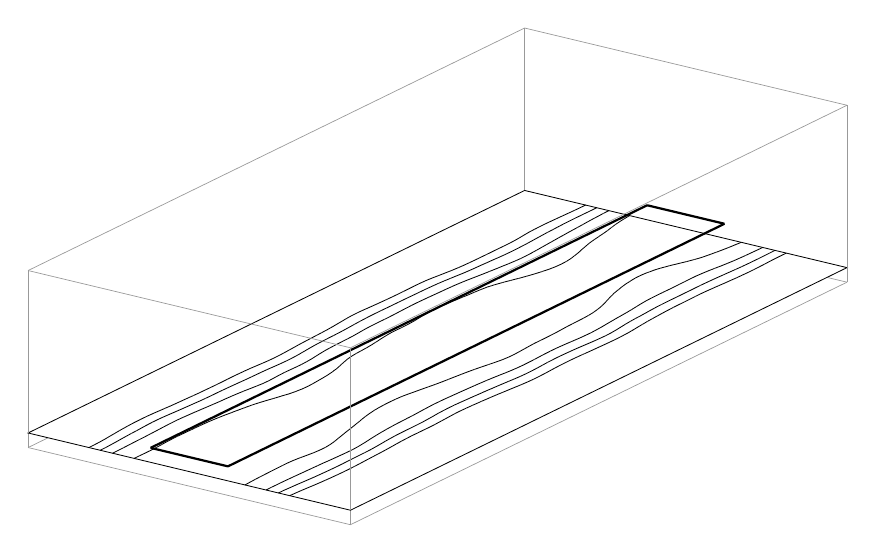
\begin{tikzpicture}
% generated by report/data/gen.py, do not edit
\draw[line width=0.25pt, black!40] (63.06mm,40.61mm) -- (63.06mm,42.45mm);
\draw[line width=0.25pt, black!40] (63.06mm,40.61mm) -- (104.00mm,30.80mm);
\draw[line width=0.25pt, black!40] (63.06mm,40.61mm) -- (0.00mm,9.80mm);
\draw[line width=0.25pt, black!40] (104.00mm,30.80mm) -- (104.00mm,32.65mm);
\draw[line width=0.25pt, black!40] (104.00mm,30.80mm) -- (40.94mm,0.00mm);
\draw[line width=0.25pt, black!40] (0.00mm,9.80mm) -- (0.00mm,11.65mm);
\draw[line width=0.25pt, black!40] (0.00mm,9.80mm) -- (40.94mm,0.00mm);
\draw[line width=0.25pt, black!40] (40.94mm,0.00mm) -- (40.94mm,1.84mm);
\filldraw[fill=white, draw=black, line width=0.30pt] (63.06mm,42.45mm) -- (0.00mm,11.65mm) -- (40.94mm,1.84mm) -- (104.00mm,32.65mm) -- cycle;
\draw[line width=0.30pt] (50.54mm,31.01mm) -- (50.93mm,31.17mm);
\draw[line width=0.30pt] (49.79mm,30.67mm) -- (50.54mm,31.01mm);
\draw[line width=0.30pt] (49.08mm,30.33mm) -- (49.79mm,30.67mm);
\draw[line width=0.30pt] (48.38mm,29.98mm) -- (49.08mm,30.33mm);
\draw[line width=0.30pt] (47.68mm,29.63mm) -- (48.38mm,29.98mm);
\draw[line width=0.30pt] (46.97mm,29.28mm) -- (47.68mm,29.63mm);
\draw[line width=0.30pt] (46.26mm,28.94mm) -- (46.97mm,29.28mm);
\draw[line width=0.30pt] (45.53mm,28.60mm) -- (46.26mm,28.94mm);
\draw[line width=0.30pt] (44.80mm,28.26mm) -- (45.53mm,28.60mm);
\draw[line width=0.30pt] (44.05mm,27.92mm) -- (44.80mm,28.26mm);
\draw[line width=0.30pt] (43.29mm,27.58mm) -- (44.05mm,27.92mm);
\draw[line width=0.30pt] (42.54mm,27.25mm) -- (43.29mm,27.58mm);
\draw[line width=0.30pt] (41.81mm,26.91mm) -- (42.54mm,27.25mm);
\draw[line width=0.30pt] (41.11mm,26.56mm) -- (41.81mm,26.91mm);
\draw[line width=0.30pt] (40.46mm,26.20mm) -- (41.11mm,26.56mm);
\draw[line width=0.30pt] (39.84mm,25.83mm) -- (40.46mm,26.20mm);
\draw[line width=0.30pt] (39.22mm,25.47mm) -- (39.84mm,25.83mm);
\draw[line width=0.30pt] (39.00mm,25.34mm) -- (39.22mm,25.47mm);
\draw[line width=0.30pt] (17.27mm,14.73mm) -- (17.35mm,14.77mm);
\draw[line width=0.30pt] (16.51mm,14.40mm) -- (17.27mm,14.73mm);
\draw[line width=0.30pt] (15.75mm,14.07mm) -- (16.51mm,14.40mm);
\draw[line width=0.30pt] (15.01mm,13.73mm) -- (15.75mm,14.07mm);
\draw[line width=0.30pt] (14.29mm,13.38mm) -- (15.01mm,13.73mm);
\draw[line width=0.30pt] (13.59mm,13.03mm) -- (14.29mm,13.38mm);
\draw[line width=0.30pt] (12.92mm,12.68mm) -- (13.59mm,13.03mm);
\draw[line width=0.30pt] (12.26mm,12.32mm) -- (12.92mm,12.68mm);
\draw[line width=0.30pt] (11.68mm,11.99mm) -- (12.26mm,12.32mm);
\draw[line width=0.30pt] (70.09mm,40.25mm) -- (70.80mm,40.60mm);
\draw[line width=0.30pt] (69.37mm,39.91mm) -- (70.09mm,40.25mm);
\draw[line width=0.30pt] (68.63mm,39.57mm) -- (69.37mm,39.91mm);
\draw[line width=0.30pt] (67.89mm,39.23mm) -- (68.63mm,39.57mm);
\draw[line width=0.30pt] (67.15mm,38.89mm) -- (67.89mm,39.23mm);
\draw[line width=0.30pt] (66.42mm,38.55mm) -- (67.15mm,38.89mm);
\draw[line width=0.30pt] (65.69mm,38.21mm) -- (66.42mm,38.55mm);
\draw[line width=0.30pt] (64.99mm,37.86mm) -- (65.69mm,38.21mm);
\draw[line width=0.30pt] (64.30mm,37.51mm) -- (64.99mm,37.86mm);
\draw[line width=0.30pt] (63.63mm,37.16mm) -- (64.30mm,37.51mm);
\draw[line width=0.30pt] (63.00mm,36.79mm) -- (63.63mm,37.16mm);
\draw[line width=0.30pt] (62.39mm,36.43mm) -- (63.00mm,36.79mm);
\draw[line width=0.30pt] (54.58mm,32.62mm) -- (54.68mm,32.66mm);
\draw[line width=0.30pt] (53.79mm,32.29mm) -- (54.58mm,32.62mm);
\draw[line width=0.30pt] (52.98mm,31.97mm) -- (53.79mm,32.29mm);
\draw[line width=0.30pt] (52.15mm,31.65mm) -- (52.98mm,31.97mm);
\draw[line width=0.30pt] (51.33mm,31.33mm) -- (52.15mm,31.65mm);
\draw[line width=0.30pt] (50.93mm,31.17mm) -- (51.33mm,31.33mm);
\draw[line width=0.30pt] (39.00mm,25.34mm) -- (38.59mm,25.10mm);
\draw[line width=0.30pt] (37.94mm,24.74mm) -- (38.59mm,25.10mm);
\draw[line width=0.30pt] (37.27mm,24.38mm) -- (37.94mm,24.74mm);
\draw[line width=0.30pt] (36.60mm,24.03mm) -- (37.27mm,24.38mm);
\draw[line width=0.30pt] (35.93mm,23.68mm) -- (36.60mm,24.03mm);
\draw[line width=0.30pt] (35.25mm,23.32mm) -- (35.93mm,23.68mm);
\draw[line width=0.30pt] (34.58mm,22.97mm) -- (35.25mm,23.32mm);
\draw[line width=0.30pt] (33.93mm,22.61mm) -- (34.58mm,22.97mm);
\draw[line width=0.30pt] (33.28mm,22.25mm) -- (33.93mm,22.61mm);
\draw[line width=0.30pt] (32.64mm,21.90mm) -- (33.28mm,22.25mm);
\draw[line width=0.30pt] (29.77mm,20.51mm) -- (30.07mm,20.64mm);
\draw[line width=0.30pt] (28.99mm,20.18mm) -- (29.77mm,20.51mm);
\draw[line width=0.30pt] (28.22mm,19.85mm) -- (28.99mm,20.18mm);
\draw[line width=0.30pt] (27.47mm,19.51mm) -- (28.22mm,19.85mm);
\draw[line width=0.30pt] (26.74mm,19.17mm) -- (27.47mm,19.51mm);
\draw[line width=0.30pt] (26.02mm,18.83mm) -- (26.74mm,19.17mm);
\draw[line width=0.30pt] (25.32mm,18.48mm) -- (26.02mm,18.83mm);
\draw[line width=0.30pt] (24.62mm,18.13mm) -- (25.32mm,18.48mm);
\draw[line width=0.30pt] (23.91mm,17.78mm) -- (24.62mm,18.13mm);
\draw[line width=0.30pt] (23.20mm,17.44mm) -- (23.91mm,17.78mm);
\draw[line width=0.30pt] (22.48mm,17.10mm) -- (23.20mm,17.44mm);
\draw[line width=0.30pt] (21.75mm,16.75mm) -- (22.48mm,17.10mm);
\draw[line width=0.30pt] (21.01mm,16.41mm) -- (21.75mm,16.75mm);
\draw[line width=0.30pt] (20.27mm,16.08mm) -- (21.01mm,16.41mm);
\draw[line width=0.30pt] (19.53mm,15.74mm) -- (20.27mm,16.08mm);
\draw[line width=0.30pt] (18.79mm,15.40mm) -- (19.53mm,15.74mm);
\draw[line width=0.30pt] (18.04mm,15.06mm) -- (18.79mm,15.40mm);
\draw[line width=0.30pt] (17.35mm,14.77mm) -- (18.04mm,15.06mm);
\draw[line width=0.30pt] (11.68mm,11.99mm) -- (11.62mm,11.96mm);
\draw[line width=0.30pt] (10.99mm,11.59mm) -- (11.62mm,11.96mm);
\draw[line width=0.30pt] (10.37mm,11.23mm) -- (10.99mm,11.59mm);
\draw[line width=0.30pt] (9.74mm,10.86mm) -- (10.37mm,11.23mm);
\draw[line width=0.30pt] (9.09mm,10.50mm) -- (9.74mm,10.86mm);
\draw[line width=0.30pt] (8.42mm,10.15mm) -- (9.09mm,10.50mm);
\draw[line width=0.30pt] (7.73mm,9.80mm) -- (8.42mm,10.15mm);
\draw[line width=0.30pt] (62.39mm,36.43mm) -- (62.38mm,36.42mm);
\draw[line width=0.30pt] (61.74mm,36.06mm) -- (62.38mm,36.42mm);
\draw[line width=0.30pt] (61.07mm,35.71mm) -- (61.74mm,36.06mm);
\draw[line width=0.30pt] (60.36mm,35.36mm) -- (61.07mm,35.71mm);
\draw[line width=0.30pt] (59.65mm,35.02mm) -- (60.36mm,35.36mm);
\draw[line width=0.30pt] (58.94mm,34.67mm) -- (59.65mm,35.02mm);
\draw[line width=0.30pt] (58.23mm,34.32mm) -- (58.94mm,34.67mm);
\draw[line width=0.30pt] (57.51mm,33.98mm) -- (58.23mm,34.32mm);
\draw[line width=0.30pt] (56.80mm,33.63mm) -- (57.51mm,33.98mm);
\draw[line width=0.30pt] (56.07mm,33.29mm) -- (56.80mm,33.63mm);
\draw[line width=0.30pt] (55.34mm,32.95mm) -- (56.07mm,33.29mm);
\draw[line width=0.30pt] (54.68mm,32.66mm) -- (55.34mm,32.95mm);
\draw[line width=0.30pt] (32.64mm,21.90mm) -- (32.62mm,21.89mm);
\draw[line width=0.30pt] (31.95mm,21.53mm) -- (32.62mm,21.89mm);
\draw[line width=0.30pt] (31.25mm,21.18mm) -- (31.95mm,21.53mm);
\draw[line width=0.30pt] (30.52mm,20.84mm) -- (31.25mm,21.18mm);
\draw[line width=0.30pt] (30.07mm,20.64mm) -- (30.52mm,20.84mm);
\draw[line width=0.30pt] (86.95mm,30.02mm) -- (87.23mm,30.15mm);
\draw[line width=0.30pt] (86.20mm,29.69mm) -- (86.95mm,30.02mm);
\draw[line width=0.30pt] (85.47mm,29.35mm) -- (86.20mm,29.69mm);
\draw[line width=0.30pt] (84.76mm,29.00mm) -- (85.47mm,29.35mm);
\draw[line width=0.30pt] (84.06mm,28.65mm) -- (84.76mm,29.00mm);
\draw[line width=0.30pt] (83.37mm,28.30mm) -- (84.06mm,28.65mm);
\draw[line width=0.30pt] (82.67mm,27.96mm) -- (83.37mm,28.30mm);
\draw[line width=0.30pt] (81.97mm,27.61mm) -- (82.67mm,27.96mm);
\draw[line width=0.30pt] (81.28mm,27.25mm) -- (81.97mm,27.61mm);
\draw[line width=0.30pt] (81.01mm,27.11mm) -- (81.28mm,27.25mm);
\draw[line width=0.30pt] (57.18mm,15.49mm) -- (57.58mm,15.67mm);
\draw[line width=0.30pt] (56.43mm,15.16mm) -- (57.18mm,15.49mm);
\draw[line width=0.30pt] (55.68mm,14.82mm) -- (56.43mm,15.16mm);
\draw[line width=0.30pt] (54.95mm,14.48mm) -- (55.68mm,14.82mm);
\draw[line width=0.30pt] (54.25mm,14.13mm) -- (54.95mm,14.48mm);
\draw[line width=0.30pt] (53.58mm,13.77mm) -- (54.25mm,14.13mm);
\draw[line width=0.30pt] (52.92mm,13.41mm) -- (53.58mm,13.77mm);
\draw[line width=0.30pt] (52.53mm,13.20mm) -- (52.92mm,13.41mm);
\draw[line width=0.30pt] (95.58mm,34.15mm) -- (96.29mm,34.49mm);
\draw[line width=0.30pt] (94.88mm,33.80mm) -- (95.58mm,34.15mm);
\draw[line width=0.30pt] (94.20mm,33.45mm) -- (94.88mm,33.80mm);
\draw[line width=0.30pt] (93.52mm,33.09mm) -- (94.20mm,33.45mm);
\draw[line width=0.30pt] (92.84mm,32.74mm) -- (93.52mm,33.09mm);
\draw[line width=0.30pt] (92.15mm,32.39mm) -- (92.84mm,32.74mm);
\draw[line width=0.30pt] (91.44mm,32.04mm) -- (92.15mm,32.39mm);
\draw[line width=0.30pt] (90.71mm,31.70mm) -- (91.44mm,32.04mm);
\draw[line width=0.30pt] (89.98mm,31.36mm) -- (90.71mm,31.70mm);
\draw[line width=0.30pt] (89.23mm,31.03mm) -- (89.98mm,31.36mm);
\draw[line width=0.30pt] (88.48mm,30.69mm) -- (89.23mm,31.03mm);
\draw[line width=0.30pt] (87.71mm,30.36mm) -- (88.48mm,30.69mm);
\draw[line width=0.30pt] (87.23mm,30.15mm) -- (87.71mm,30.36mm);
\draw[line width=0.30pt] (81.01mm,27.11mm) -- (80.62mm,26.90mm);
\draw[line width=0.30pt] (79.96mm,26.54mm) -- (80.62mm,26.90mm);
\draw[line width=0.30pt] (79.30mm,26.18mm) -- (79.96mm,26.54mm);
\draw[line width=0.30pt] (78.66mm,25.82mm) -- (79.30mm,26.18mm);
\draw[line width=0.30pt] (78.03mm,25.45mm) -- (78.66mm,25.82mm);
\draw[line width=0.30pt] (77.42mm,25.09mm) -- (78.03mm,25.45mm);
\draw[line width=0.30pt] (76.83mm,24.73mm) -- (77.42mm,25.09mm);
\draw[line width=0.30pt] (70.41mm,21.61mm) -- (70.66mm,21.72mm);
\draw[line width=0.30pt] (69.67mm,21.27mm) -- (70.41mm,21.61mm);
\draw[line width=0.30pt] (68.94mm,20.93mm) -- (69.67mm,21.27mm);
\draw[line width=0.30pt] (68.23mm,20.58mm) -- (68.94mm,20.93mm);
\draw[line width=0.30pt] (67.54mm,20.23mm) -- (68.23mm,20.58mm);
\draw[line width=0.30pt] (66.87mm,19.88mm) -- (67.54mm,20.23mm);
\draw[line width=0.30pt] (66.67mm,19.77mm) -- (66.87mm,19.88mm);
\draw[line width=0.30pt] (61.86mm,17.47mm) -- (62.50mm,17.73mm);
\draw[line width=0.30pt] (61.06mm,17.14mm) -- (61.86mm,17.47mm);
\draw[line width=0.30pt] (60.27mm,16.81mm) -- (61.06mm,17.14mm);
\draw[line width=0.30pt] (59.48mm,16.49mm) -- (60.27mm,16.81mm);
\draw[line width=0.30pt] (58.71mm,16.16mm) -- (59.48mm,16.49mm);
\draw[line width=0.30pt] (57.94mm,15.82mm) -- (58.71mm,16.16mm);
\draw[line width=0.30pt] (57.58mm,15.67mm) -- (57.94mm,15.82mm);
\draw[line width=0.30pt] (52.53mm,13.20mm) -- (52.27mm,13.06mm);
\draw[line width=0.30pt] (51.60mm,12.70mm) -- (52.27mm,13.06mm);
\draw[line width=0.30pt] (50.91mm,12.35mm) -- (51.60mm,12.70mm);
\draw[line width=0.30pt] (50.20mm,12.01mm) -- (50.91mm,12.35mm);
\draw[line width=0.30pt] (49.48mm,11.66mm) -- (50.20mm,12.01mm);
\draw[line width=0.30pt] (48.77mm,11.32mm) -- (49.48mm,11.66mm);
\draw[line width=0.30pt] (48.08mm,10.96mm) -- (48.77mm,11.32mm);
\draw[line width=0.30pt] (47.41mm,10.61mm) -- (48.08mm,10.96mm);
\draw[line width=0.30pt] (46.76mm,10.25mm) -- (47.41mm,10.61mm);
\draw[line width=0.30pt] (46.12mm,9.89mm) -- (46.76mm,10.25mm);
\draw[line width=0.30pt] (45.47mm,9.53mm) -- (46.12mm,9.89mm);
\draw[line width=0.30pt] (44.80mm,9.17mm) -- (45.47mm,9.53mm);
\draw[line width=0.30pt] (44.13mm,8.82mm) -- (44.80mm,9.17mm);
\draw[line width=0.30pt] (43.45mm,8.46mm) -- (44.13mm,8.82mm);
\draw[line width=0.30pt] (42.78mm,8.11mm) -- (43.45mm,8.46mm);
\draw[line width=0.30pt] (42.58mm,8.00mm) -- (42.78mm,8.11mm);
\draw[line width=0.30pt] (37.08mm,5.35mm) -- (37.78mm,5.66mm);
\draw[line width=0.30pt] (36.31mm,5.02mm) -- (37.08mm,5.35mm);
\draw[line width=0.30pt] (35.52mm,4.69mm) -- (36.31mm,5.02mm);
\draw[line width=0.30pt] (34.74mm,4.36mm) -- (35.52mm,4.69mm);
\draw[line width=0.30pt] (33.98mm,4.03mm) -- (34.74mm,4.36mm);
\draw[line width=0.30pt] (33.23mm,3.69mm) -- (33.98mm,4.03mm);
\draw[line width=0.30pt] (76.83mm,24.73mm) -- (76.81mm,24.72mm);
\draw[line width=0.30pt] (76.17mm,24.35mm) -- (76.81mm,24.72mm);
\draw[line width=0.30pt] (75.51mm,24.00mm) -- (76.17mm,24.35mm);
\draw[line width=0.30pt] (74.82mm,23.64mm) -- (75.51mm,24.00mm);
\draw[line width=0.30pt] (74.11mm,23.30mm) -- (74.82mm,23.64mm);
\draw[line width=0.30pt] (73.38mm,22.96mm) -- (74.11mm,23.30mm);
\draw[line width=0.30pt] (72.64mm,22.62mm) -- (73.38mm,22.96mm);
\draw[line width=0.30pt] (71.90mm,22.28mm) -- (72.64mm,22.62mm);
\draw[line width=0.30pt] (71.16mm,21.94mm) -- (71.90mm,22.28mm);
\draw[line width=0.30pt] (70.66mm,21.72mm) -- (71.16mm,21.94mm);
\draw[line width=0.30pt] (66.67mm,19.77mm) -- (66.21mm,19.52mm);
\draw[line width=0.30pt] (65.54mm,19.16mm) -- (66.21mm,19.52mm);
\draw[line width=0.30pt] (64.86mm,18.81mm) -- (65.54mm,19.16mm);
\draw[line width=0.30pt] (64.15mm,18.46mm) -- (64.86mm,18.81mm);
\draw[line width=0.30pt] (63.41mm,18.12mm) -- (64.15mm,18.46mm);
\draw[line width=0.30pt] (62.64mm,17.79mm) -- (63.41mm,18.12mm);
\draw[line width=0.30pt] (62.50mm,17.73mm) -- (62.64mm,17.79mm);
\draw[line width=0.30pt] (42.58mm,8.00mm) -- (42.11mm,7.75mm);
\draw[line width=0.30pt] (41.44mm,7.40mm) -- (42.11mm,7.75mm);
\draw[line width=0.30pt] (40.75mm,7.05mm) -- (41.44mm,7.40mm);
\draw[line width=0.30pt] (40.04mm,6.70mm) -- (40.75mm,7.05mm);
\draw[line width=0.30pt] (39.31mm,6.36mm) -- (40.04mm,6.70mm);
\draw[line width=0.30pt] (38.58mm,6.02mm) -- (39.31mm,6.36mm);
\draw[line width=0.30pt] (37.83mm,5.68mm) -- (38.58mm,6.02mm);
\draw[line width=0.30pt] (37.78mm,5.66mm) -- (37.83mm,5.68mm);
\draw[line width=0.30pt] (44.87mm,27.21mm) -- (45.51mm,27.52mm);
\draw[line width=0.30pt] (44.15mm,26.86mm) -- (44.87mm,27.21mm);
\draw[line width=0.30pt] (43.45mm,26.51mm) -- (44.15mm,26.86mm);
\draw[line width=0.30pt] (43.28mm,26.43mm) -- (43.45mm,26.51mm);
\draw[line width=0.30pt] (17.24mm,13.71mm) -- (17.25mm,13.71mm);
\draw[line width=0.30pt] (16.50mm,13.37mm) -- (17.24mm,13.71mm);
\draw[line width=0.30pt] (15.79mm,13.02mm) -- (16.50mm,13.37mm);
\draw[line width=0.30pt] (15.11mm,12.67mm) -- (15.79mm,13.02mm);
\draw[line width=0.30pt] (15.08mm,12.65mm) -- (15.11mm,12.67mm);
\draw[line width=0.30pt] (71.51mm,39.91mm) -- (72.22mm,40.26mm);
\draw[line width=0.30pt] (70.80mm,39.57mm) -- (71.51mm,39.91mm);
\draw[line width=0.30pt] (70.08mm,39.22mm) -- (70.80mm,39.57mm);
\draw[line width=0.30pt] (69.37mm,38.88mm) -- (70.08mm,39.22mm);
\draw[line width=0.30pt] (68.67mm,38.53mm) -- (69.37mm,38.88mm);
\draw[line width=0.30pt] (67.98mm,38.18mm) -- (68.67mm,38.53mm);
\draw[line width=0.30pt] (67.30mm,37.82mm) -- (67.98mm,38.18mm);
\draw[line width=0.30pt] (67.29mm,37.82mm) -- (67.30mm,37.82mm);
\draw[line width=0.30pt] (55.25mm,31.94mm) -- (55.34mm,31.98mm);
\draw[line width=0.30pt] (54.45mm,31.62mm) -- (55.25mm,31.94mm);
\draw[line width=0.30pt] (53.65mm,31.29mm) -- (54.45mm,31.62mm);
\draw[line width=0.30pt] (52.86mm,30.97mm) -- (53.65mm,31.29mm);
\draw[line width=0.30pt] (52.09mm,30.64mm) -- (52.86mm,30.97mm);
\draw[line width=0.30pt] (51.34mm,30.30mm) -- (52.09mm,30.64mm);
\draw[line width=0.30pt] (50.60mm,29.96mm) -- (51.34mm,30.30mm);
\draw[line width=0.30pt] (49.88mm,29.62mm) -- (50.60mm,29.96mm);
\draw[line width=0.30pt] (49.16mm,29.27mm) -- (49.88mm,29.62mm);
\draw[line width=0.30pt] (48.44mm,28.93mm) -- (49.16mm,29.27mm);
\draw[line width=0.30pt] (47.73mm,28.59mm) -- (48.44mm,28.93mm);
\draw[line width=0.30pt] (47.01mm,28.24mm) -- (47.73mm,28.59mm);
\draw[line width=0.30pt] (46.30mm,27.90mm) -- (47.01mm,28.24mm);
\draw[line width=0.30pt] (45.59mm,27.55mm) -- (46.30mm,27.90mm);
\draw[line width=0.30pt] (45.51mm,27.52mm) -- (45.59mm,27.55mm);
\draw[line width=0.30pt] (43.28mm,26.43mm) -- (42.77mm,26.16mm);
\draw[line width=0.30pt] (42.10mm,25.81mm) -- (42.77mm,26.16mm);
\draw[line width=0.30pt] (41.45mm,25.45mm) -- (42.10mm,25.81mm);
\draw[line width=0.30pt] (40.80mm,25.09mm) -- (41.45mm,25.45mm);
\draw[line width=0.30pt] (40.14mm,24.73mm) -- (40.80mm,25.09mm);
\draw[line width=0.30pt] (39.47mm,24.37mm) -- (40.14mm,24.73mm);
\draw[line width=0.30pt] (38.78mm,24.02mm) -- (39.47mm,24.37mm);
\draw[line width=0.30pt] (38.09mm,23.67mm) -- (38.78mm,24.02mm);
\draw[line width=0.30pt] (37.41mm,23.32mm) -- (38.09mm,23.67mm);
\draw[line width=0.30pt] (36.73mm,22.97mm) -- (37.41mm,23.32mm);
\draw[line width=0.30pt] (36.08mm,22.61mm) -- (36.73mm,22.97mm);
\draw[line width=0.30pt] (35.68mm,22.38mm) -- (36.08mm,22.61mm);
\draw[line width=0.30pt] (26.90mm,18.10mm) -- (27.13mm,18.20mm);
\draw[line width=0.30pt] (26.16mm,17.76mm) -- (26.90mm,18.10mm);
\draw[line width=0.30pt] (25.42mm,17.42mm) -- (26.16mm,17.76mm);
\draw[line width=0.30pt] (24.69mm,17.08mm) -- (25.42mm,17.42mm);
\draw[line width=0.30pt] (23.97mm,16.74mm) -- (24.69mm,17.08mm);
\draw[line width=0.30pt] (23.26mm,16.39mm) -- (23.97mm,16.74mm);
\draw[line width=0.30pt] (22.54mm,16.05mm) -- (23.26mm,16.39mm);
\draw[line width=0.30pt] (21.80mm,15.71mm) -- (22.54mm,16.05mm);
\draw[line width=0.30pt] (21.05mm,15.38mm) -- (21.80mm,15.71mm);
\draw[line width=0.30pt] (20.29mm,15.04mm) -- (21.05mm,15.38mm);
\draw[line width=0.30pt] (19.54mm,14.71mm) -- (20.29mm,15.04mm);
\draw[line width=0.30pt] (18.77mm,14.37mm) -- (19.54mm,14.71mm);
\draw[line width=0.30pt] (18.00mm,14.04mm) -- (18.77mm,14.37mm);
\draw[line width=0.30pt] (17.25mm,13.71mm) -- (18.00mm,14.04mm);
\draw[line width=0.30pt] (15.08mm,12.65mm) -- (14.45mm,12.31mm);
\draw[line width=0.30pt] (13.80mm,11.95mm) -- (14.45mm,12.31mm);
\draw[line width=0.30pt] (13.13mm,11.60mm) -- (13.80mm,11.95mm);
\draw[line width=0.30pt] (12.47mm,11.24mm) -- (13.13mm,11.60mm);
\draw[line width=0.30pt] (11.82mm,10.88mm) -- (12.47mm,11.24mm);
\draw[line width=0.30pt] (11.18mm,10.52mm) -- (11.82mm,10.88mm);
\draw[line width=0.30pt] (10.52mm,10.16mm) -- (11.18mm,10.52mm);
\draw[line width=0.30pt] (9.85mm,9.80mm) -- (10.52mm,10.16mm);
\draw[line width=0.30pt] (9.16mm,9.45mm) -- (9.85mm,9.80mm);
\draw[line width=0.30pt] (67.29mm,37.82mm) -- (66.63mm,37.47mm);
\draw[line width=0.30pt] (65.95mm,37.12mm) -- (66.63mm,37.47mm);
\draw[line width=0.30pt] (65.29mm,36.76mm) -- (65.95mm,37.12mm);
\draw[line width=0.30pt] (64.63mm,36.40mm) -- (65.29mm,36.76mm);
\draw[line width=0.30pt] (63.97mm,36.04mm) -- (64.63mm,36.40mm);
\draw[line width=0.30pt] (63.31mm,35.68mm) -- (63.97mm,36.04mm);
\draw[line width=0.30pt] (62.64mm,35.33mm) -- (63.31mm,35.68mm);
\draw[line width=0.30pt] (61.96mm,34.98mm) -- (62.64mm,35.33mm);
\draw[line width=0.30pt] (61.25mm,34.63mm) -- (61.96mm,34.98mm);
\draw[line width=0.30pt] (60.53mm,34.29mm) -- (61.25mm,34.63mm);
\draw[line width=0.30pt] (59.78mm,33.95mm) -- (60.53mm,34.29mm);
\draw[line width=0.30pt] (59.02mm,33.62mm) -- (59.78mm,33.95mm);
\draw[line width=0.30pt] (58.27mm,33.28mm) -- (59.02mm,33.62mm);
\draw[line width=0.30pt] (57.52mm,32.95mm) -- (58.27mm,33.28mm);
\draw[line width=0.30pt] (56.78mm,32.61mm) -- (57.52mm,32.95mm);
\draw[line width=0.30pt] (56.02mm,32.27mm) -- (56.78mm,32.61mm);
\draw[line width=0.30pt] (55.34mm,31.98mm) -- (56.02mm,32.27mm);
\draw[line width=0.30pt] (35.68mm,22.38mm) -- (35.44mm,22.24mm);
\draw[line width=0.30pt] (34.82mm,21.88mm) -- (35.44mm,22.24mm);
\draw[line width=0.30pt] (34.18mm,21.51mm) -- (34.82mm,21.88mm);
\draw[line width=0.30pt] (33.52mm,21.16mm) -- (34.18mm,21.51mm);
\draw[line width=0.30pt] (32.82mm,20.81mm) -- (33.52mm,21.16mm);
\draw[line width=0.30pt] (32.09mm,20.47mm) -- (32.82mm,20.81mm);
\draw[line width=0.30pt] (31.33mm,20.13mm) -- (32.09mm,20.47mm);
\draw[line width=0.30pt] (30.57mm,19.80mm) -- (31.33mm,20.13mm);
\draw[line width=0.30pt] (29.82mm,19.46mm) -- (30.57mm,19.80mm);
\draw[line width=0.30pt] (29.10mm,19.12mm) -- (29.82mm,19.46mm);
\draw[line width=0.30pt] (28.38mm,18.78mm) -- (29.10mm,19.12mm);
\draw[line width=0.30pt] (27.65mm,18.44mm) -- (28.38mm,18.78mm);
\draw[line width=0.30pt] (27.13mm,18.20mm) -- (27.65mm,18.44mm);
\draw[line width=0.30pt] (89.10mm,32.09mm) -- (89.69mm,32.35mm);
\draw[line width=0.30pt] (88.34mm,31.75mm) -- (89.10mm,32.09mm);
\draw[line width=0.30pt] (87.60mm,31.42mm) -- (88.34mm,31.75mm);
\draw[line width=0.30pt] (86.85mm,31.08mm) -- (87.60mm,31.42mm);
\draw[line width=0.30pt] (86.12mm,30.74mm) -- (86.85mm,31.08mm);
\draw[line width=0.30pt] (85.40mm,30.40mm) -- (86.12mm,30.74mm);
\draw[line width=0.30pt] (84.69mm,30.05mm) -- (85.40mm,30.40mm);
\draw[line width=0.30pt] (83.98mm,29.70mm) -- (84.69mm,30.05mm);
\draw[line width=0.30pt] (83.27mm,29.36mm) -- (83.98mm,29.70mm);
\draw[line width=0.30pt] (82.57mm,29.01mm) -- (83.27mm,29.36mm);
\draw[line width=0.30pt] (81.86mm,28.67mm) -- (82.57mm,29.01mm);
\draw[line width=0.30pt] (81.14mm,28.32mm) -- (81.86mm,28.67mm);
\draw[line width=0.30pt] (80.44mm,27.97mm) -- (81.14mm,28.32mm);
\draw[line width=0.30pt] (79.76mm,27.62mm) -- (80.44mm,27.97mm);
\draw[line width=0.30pt] (79.10mm,27.26mm) -- (79.76mm,27.62mm);
\draw[line width=0.30pt] (78.45mm,26.90mm) -- (79.10mm,27.26mm);
\draw[line width=0.30pt] (77.81mm,26.55mm) -- (78.45mm,26.90mm);
\draw[line width=0.30pt] (58.65mm,17.20mm) -- (58.78mm,17.25mm);
\draw[line width=0.30pt] (57.89mm,16.87mm) -- (58.65mm,17.20mm);
\draw[line width=0.30pt] (57.13mm,16.53mm) -- (57.89mm,16.87mm);
\draw[line width=0.30pt] (56.37mm,16.20mm) -- (57.13mm,16.53mm);
\draw[line width=0.30pt] (55.62mm,15.86mm) -- (56.37mm,16.20mm);
\draw[line width=0.30pt] (54.87mm,15.53mm) -- (55.62mm,15.86mm);
\draw[line width=0.30pt] (54.13mm,15.19mm) -- (54.87mm,15.53mm);
\draw[line width=0.30pt] (53.41mm,14.84mm) -- (54.13mm,15.19mm);
\draw[line width=0.30pt] (52.73mm,14.49mm) -- (53.41mm,14.84mm);
\draw[line width=0.30pt] (52.07mm,14.14mm) -- (52.73mm,14.49mm);
\draw[line width=0.30pt] (51.43mm,13.77mm) -- (52.07mm,14.14mm);
\draw[line width=0.30pt] (50.78mm,13.41mm) -- (51.43mm,13.77mm);
\draw[line width=0.30pt] (50.13mm,13.05mm) -- (50.78mm,13.41mm);
\draw[line width=0.30pt] (49.44mm,12.70mm) -- (50.13mm,13.05mm);
\draw[line width=0.30pt] (48.74mm,12.35mm) -- (49.44mm,12.70mm);
\draw[line width=0.30pt] (48.03mm,12.01mm) -- (48.74mm,12.35mm);
\draw[line width=0.30pt] (47.33mm,11.66mm) -- (48.03mm,12.01mm);
\draw[line width=0.30pt] (47.29mm,11.64mm) -- (47.33mm,11.66mm);
\draw[line width=0.30pt] (94.15mm,34.49mm) -- (94.86mm,34.84mm);
\draw[line width=0.30pt] (93.45mm,34.14mm) -- (94.15mm,34.49mm);
\draw[line width=0.30pt] (92.75mm,33.79mm) -- (93.45mm,34.14mm);
\draw[line width=0.30pt] (92.05mm,33.45mm) -- (92.75mm,33.79mm);
\draw[line width=0.30pt] (91.33mm,33.10mm) -- (92.05mm,33.45mm);
\draw[line width=0.30pt] (90.60mm,32.76mm) -- (91.33mm,33.10mm);
\draw[line width=0.30pt] (89.85mm,32.42mm) -- (90.60mm,32.76mm);
\draw[line width=0.30pt] (89.69mm,32.35mm) -- (89.85mm,32.42mm);
\draw[line width=0.30pt] (77.81mm,26.55mm) -- (77.80mm,26.54mm);
\draw[line width=0.30pt] (77.13mm,26.19mm) -- (77.80mm,26.54mm);
\draw[line width=0.30pt] (76.49mm,25.83mm) -- (77.13mm,26.19mm);
\draw[line width=0.30pt] (75.86mm,25.46mm) -- (76.49mm,25.83mm);
\draw[line width=0.30pt] (75.26mm,25.09mm) -- (75.86mm,25.46mm);
\draw[line width=0.30pt] (74.66mm,24.72mm) -- (75.26mm,25.09mm);
\draw[line width=0.30pt] (74.19mm,24.45mm) -- (74.66mm,24.72mm);
\draw[line width=0.30pt] (71.86mm,23.32mm) -- (72.21mm,23.48mm);
\draw[line width=0.30pt] (71.09mm,22.99mm) -- (71.86mm,23.32mm);
\draw[line width=0.30pt] (70.32mm,22.66mm) -- (71.09mm,22.99mm);
\draw[line width=0.30pt] (69.55mm,22.33mm) -- (70.32mm,22.66mm);
\draw[line width=0.30pt] (68.80mm,21.99mm) -- (69.55mm,22.33mm);
\draw[line width=0.30pt] (68.06mm,21.65mm) -- (68.80mm,21.99mm);
\draw[line width=0.30pt] (67.34mm,21.31mm) -- (68.06mm,21.65mm);
\draw[line width=0.30pt] (66.64mm,20.96mm) -- (67.34mm,21.31mm);
\draw[line width=0.30pt] (65.96mm,20.61mm) -- (66.64mm,20.96mm);
\draw[line width=0.30pt] (65.30mm,20.25mm) -- (65.96mm,20.61mm);
\draw[line width=0.30pt] (64.64mm,19.89mm) -- (65.30mm,20.25mm);
\draw[line width=0.30pt] (63.97mm,19.54mm) -- (64.64mm,19.89mm);
\draw[line width=0.30pt] (63.27mm,19.19mm) -- (63.97mm,19.54mm);
\draw[line width=0.30pt] (62.54mm,18.85mm) -- (63.27mm,19.19mm);
\draw[line width=0.30pt] (61.77mm,18.52mm) -- (62.54mm,18.85mm);
\draw[line width=0.30pt] (60.98mm,18.19mm) -- (61.77mm,18.52mm);
\draw[line width=0.30pt] (60.20mm,17.86mm) -- (60.98mm,18.19mm);
\draw[line width=0.30pt] (59.42mm,17.53mm) -- (60.20mm,17.86mm);
\draw[line width=0.30pt] (58.78mm,17.25mm) -- (59.42mm,17.53mm);
\draw[line width=0.30pt] (47.29mm,11.64mm) -- (46.64mm,11.31mm);
\draw[line width=0.30pt] (45.99mm,10.95mm) -- (46.64mm,11.31mm);
\draw[line width=0.30pt] (45.35mm,10.59mm) -- (45.99mm,10.95mm);
\draw[line width=0.30pt] (44.72mm,10.22mm) -- (45.35mm,10.59mm);
\draw[line width=0.30pt] (44.09mm,9.86mm) -- (44.72mm,10.22mm);
\draw[line width=0.30pt] (43.43mm,9.50mm) -- (44.09mm,9.86mm);
\draw[line width=0.30pt] (42.75mm,9.15mm) -- (43.43mm,9.50mm);
\draw[line width=0.30pt] (42.05mm,8.80mm) -- (42.75mm,9.15mm);
\draw[line width=0.30pt] (41.35mm,8.45mm) -- (42.05mm,8.80mm);
\draw[line width=0.30pt] (40.65mm,8.10mm) -- (41.35mm,8.45mm);
\draw[line width=0.30pt] (39.96mm,7.75mm) -- (40.65mm,8.10mm);
\draw[line width=0.30pt] (39.26mm,7.40mm) -- (39.96mm,7.75mm);
\draw[line width=0.30pt] (38.54mm,7.06mm) -- (39.26mm,7.40mm);
\draw[line width=0.30pt] (37.81mm,6.72mm) -- (38.54mm,7.06mm);
\draw[line width=0.30pt] (37.07mm,6.38mm) -- (37.81mm,6.72mm);
\draw[line width=0.30pt] (36.32mm,6.04mm) -- (37.07mm,6.38mm);
\draw[line width=0.30pt] (35.56mm,5.71mm) -- (36.32mm,6.04mm);
\draw[line width=0.30pt] (34.80mm,5.38mm) -- (35.56mm,5.71mm);
\draw[line width=0.30pt] (34.03mm,5.05mm) -- (34.80mm,5.38mm);
\draw[line width=0.30pt] (33.27mm,4.71mm) -- (34.03mm,5.05mm);
\draw[line width=0.30pt] (32.52mm,4.38mm) -- (33.27mm,4.71mm);
\draw[line width=0.30pt] (31.79mm,4.03mm) -- (32.52mm,4.38mm);
\draw[line width=0.30pt] (74.19mm,24.45mm) -- (74.02mm,24.35mm);
\draw[line width=0.30pt] (73.34mm,24.00mm) -- (74.02mm,24.35mm);
\draw[line width=0.30pt] (72.61mm,23.66mm) -- (73.34mm,24.00mm);
\draw[line width=0.30pt] (72.21mm,23.48mm) -- (72.61mm,23.66mm);
\draw[line width=0.30pt] (53.79mm,30.23mm) -- (54.01mm,30.33mm);
\draw[line width=0.30pt] (53.04mm,29.89mm) -- (53.79mm,30.23mm);
\draw[line width=0.30pt] (52.31mm,29.55mm) -- (53.04mm,29.89mm);
\draw[line width=0.30pt] (51.57mm,29.21mm) -- (52.31mm,29.55mm);
\draw[line width=0.30pt] (50.83mm,28.87mm) -- (51.57mm,29.21mm);
\draw[line width=0.30pt] (50.10mm,28.53mm) -- (50.83mm,28.87mm);
\draw[line width=0.30pt] (49.38mm,28.19mm) -- (50.10mm,28.53mm);
\draw[line width=0.30pt] (48.68mm,27.84mm) -- (49.38mm,28.19mm);
\draw[line width=0.30pt] (47.99mm,27.49mm) -- (48.68mm,27.84mm);
\draw[line width=0.30pt] (47.32mm,27.14mm) -- (47.99mm,27.49mm);
\draw[line width=0.30pt] (46.64mm,26.78mm) -- (47.32mm,27.14mm);
\draw[line width=0.30pt] (45.96mm,26.43mm) -- (46.64mm,26.78mm);
\draw[line width=0.30pt] (45.26mm,26.08mm) -- (45.96mm,26.43mm);
\draw[line width=0.30pt] (44.55mm,25.74mm) -- (45.26mm,26.08mm);
\draw[line width=0.30pt] (43.85mm,25.39mm) -- (44.55mm,25.74mm);
\draw[line width=0.30pt] (43.17mm,25.04mm) -- (43.85mm,25.39mm);
\draw[line width=0.30pt] (43.09mm,25.00mm) -- (43.17mm,25.04mm);
\draw[line width=0.30pt] (21.20mm,14.31mm) -- (21.27mm,14.33mm);
\draw[line width=0.30pt] (20.44mm,13.97mm) -- (21.20mm,14.31mm);
\draw[line width=0.30pt] (19.69mm,13.64mm) -- (20.44mm,13.97mm);
\draw[line width=0.30pt] (18.95mm,13.30mm) -- (19.69mm,13.64mm);
\draw[line width=0.30pt] (18.24mm,12.95mm) -- (18.95mm,13.30mm);
\draw[line width=0.30pt] (17.56mm,12.60mm) -- (18.24mm,12.95mm);
\draw[line width=0.30pt] (16.89mm,12.25mm) -- (17.56mm,12.60mm);
\draw[line width=0.30pt] (16.22mm,11.89mm) -- (16.89mm,12.25mm);
\draw[line width=0.30pt] (15.64mm,11.59mm) -- (16.22mm,11.89mm);
\draw[line width=0.30pt] (73.07mm,39.54mm) -- (73.76mm,39.89mm);
\draw[line width=0.30pt] (72.40mm,39.18mm) -- (73.07mm,39.54mm);
\draw[line width=0.30pt] (71.73mm,38.83mm) -- (72.40mm,39.18mm);
\draw[line width=0.30pt] (71.07mm,38.47mm) -- (71.73mm,38.83mm);
\draw[line width=0.30pt] (70.42mm,38.11mm) -- (71.07mm,38.47mm);
\draw[line width=0.30pt] (69.77mm,37.75mm) -- (70.42mm,38.11mm);
\draw[line width=0.30pt] (69.11mm,37.39mm) -- (69.77mm,37.75mm);
\draw[line width=0.30pt] (68.68mm,37.16mm) -- (69.11mm,37.39mm);
\draw[line width=0.30pt] (57.80mm,31.85mm) -- (57.88mm,31.88mm);
\draw[line width=0.30pt] (56.98mm,31.53mm) -- (57.80mm,31.85mm);
\draw[line width=0.30pt] (56.15mm,31.21mm) -- (56.98mm,31.53mm);
\draw[line width=0.30pt] (55.34mm,30.89mm) -- (56.15mm,31.21mm);
\draw[line width=0.30pt] (54.55mm,30.56mm) -- (55.34mm,30.89mm);
\draw[line width=0.30pt] (54.01mm,30.33mm) -- (54.55mm,30.56mm);
\draw[line width=0.30pt] (43.09mm,25.00mm) -- (42.51mm,24.68mm);
\draw[line width=0.30pt] (41.87mm,24.31mm) -- (42.51mm,24.68mm);
\draw[line width=0.30pt] (41.23mm,23.95mm) -- (41.87mm,24.31mm);
\draw[line width=0.30pt] (40.56mm,23.60mm) -- (41.23mm,23.95mm);
\draw[line width=0.30pt] (39.87mm,23.25mm) -- (40.56mm,23.60mm);
\draw[line width=0.30pt] (39.18mm,22.90mm) -- (39.87mm,23.25mm);
\draw[line width=0.30pt] (38.49mm,22.54mm) -- (39.18mm,22.90mm);
\draw[line width=0.30pt] (37.84mm,22.19mm) -- (38.49mm,22.54mm);
\draw[line width=0.30pt] (37.22mm,21.82mm) -- (37.84mm,22.19mm);
\draw[line width=0.30pt] (36.99mm,21.68mm) -- (37.22mm,21.82mm);
\draw[line width=0.30pt] (26.56mm,16.63mm) -- (27.20mm,16.89mm);
\draw[line width=0.30pt] (25.79mm,16.30mm) -- (26.56mm,16.63mm);
\draw[line width=0.30pt] (25.04mm,15.97mm) -- (25.79mm,16.30mm);
\draw[line width=0.30pt] (24.29mm,15.63mm) -- (25.04mm,15.97mm);
\draw[line width=0.30pt] (23.53mm,15.30mm) -- (24.29mm,15.63mm);
\draw[line width=0.30pt] (22.76mm,14.97mm) -- (23.53mm,15.30mm);
\draw[line width=0.30pt] (21.98mm,14.64mm) -- (22.76mm,14.97mm);
\draw[line width=0.30pt] (21.27mm,14.33mm) -- (21.98mm,14.64mm);
\draw[line width=0.30pt] (15.64mm,11.59mm) -- (15.54mm,11.54mm);
\draw[line width=0.30pt] (14.86mm,11.18mm) -- (15.54mm,11.54mm);
\draw[line width=0.30pt] (14.16mm,10.83mm) -- (14.86mm,11.18mm);
\draw[line width=0.30pt] (13.48mm,10.48mm) -- (14.16mm,10.83mm);
\draw[line width=0.30pt] (12.80mm,10.13mm) -- (13.48mm,10.48mm);
\draw[line width=0.30pt] (12.12mm,9.78mm) -- (12.80mm,10.13mm);
\draw[line width=0.30pt] (11.43mm,9.43mm) -- (12.12mm,9.78mm);
\draw[line width=0.30pt] (10.73mm,9.08mm) -- (11.43mm,9.43mm);
\draw[line width=0.30pt] (68.68mm,37.16mm) -- (68.45mm,37.03mm);
\draw[line width=0.30pt] (67.80mm,36.67mm) -- (68.45mm,37.03mm);
\draw[line width=0.30pt] (67.15mm,36.31mm) -- (67.80mm,36.67mm);
\draw[line width=0.30pt] (66.51mm,35.95mm) -- (67.15mm,36.31mm);
\draw[line width=0.30pt] (65.87mm,35.59mm) -- (66.51mm,35.95mm);
\draw[line width=0.30pt] (65.23mm,35.23mm) -- (65.87mm,35.59mm);
\draw[line width=0.30pt] (64.58mm,34.86mm) -- (65.23mm,35.23mm);
\draw[line width=0.30pt] (63.93mm,34.51mm) -- (64.58mm,34.86mm);
\draw[line width=0.30pt] (63.91mm,34.49mm) -- (63.93mm,34.51mm);
\draw[line width=0.30pt] (61.80mm,33.47mm) -- (62.01mm,33.56mm);
\draw[line width=0.30pt] (61.01mm,33.14mm) -- (61.80mm,33.47mm);
\draw[line width=0.30pt] (60.21mm,32.82mm) -- (61.01mm,33.14mm);
\draw[line width=0.30pt] (59.41mm,32.49mm) -- (60.21mm,32.82mm);
\draw[line width=0.30pt] (58.61mm,32.17mm) -- (59.41mm,32.49mm);
\draw[line width=0.30pt] (57.88mm,31.88mm) -- (58.61mm,32.17mm);
\draw[line width=0.30pt] (36.99mm,21.68mm) -- (36.62mm,21.45mm);
\draw[line width=0.30pt] (36.02mm,21.07mm) -- (36.62mm,21.45mm);
\draw[line width=0.30pt] (35.39mm,20.71mm) -- (36.02mm,21.07mm);
\draw[line width=0.30pt] (34.72mm,20.35mm) -- (35.39mm,20.71mm);
\draw[line width=0.30pt] (34.01mm,20.01mm) -- (34.72mm,20.35mm);
\draw[line width=0.30pt] (33.27mm,19.67mm) -- (34.01mm,20.01mm);
\draw[line width=0.30pt] (32.55mm,19.33mm) -- (33.27mm,19.67mm);
\draw[line width=0.30pt] (31.86mm,18.98mm) -- (32.55mm,19.33mm);
\draw[line width=0.30pt] (31.20mm,18.62mm) -- (31.86mm,18.98mm);
\draw[line width=0.30pt] (30.52mm,18.26mm) -- (31.20mm,18.62mm);
\draw[line width=0.30pt] (29.79mm,17.92mm) -- (30.52mm,18.26mm);
\draw[line width=0.30pt] (29.00mm,17.60mm) -- (29.79mm,17.92mm);
\draw[line width=0.30pt] (28.18mm,17.28mm) -- (29.00mm,17.60mm);
\draw[line width=0.30pt] (27.36mm,16.96mm) -- (28.18mm,17.28mm);
\draw[line width=0.30pt] (27.20mm,16.89mm) -- (27.36mm,16.96mm);
\draw[line width=0.30pt] (63.91mm,34.49mm) -- (63.26mm,34.15mm);
\draw[line width=0.30pt] (62.55mm,33.80mm) -- (63.26mm,34.15mm);
\draw[line width=0.30pt] (62.01mm,33.56mm) -- (62.55mm,33.80mm);
\draw[line width=0.30pt] (87.18mm,32.55mm) -- (87.96mm,32.85mm);
\draw[line width=0.30pt] (86.36mm,32.23mm) -- (87.18mm,32.55mm);
\draw[line width=0.30pt] (85.57mm,31.90mm) -- (86.36mm,32.23mm);
\draw[line width=0.30pt] (84.81mm,31.57mm) -- (85.57mm,31.90mm);
\draw[line width=0.30pt] (84.09mm,31.22mm) -- (84.81mm,31.57mm);
\draw[line width=0.30pt] (83.40mm,30.87mm) -- (84.09mm,31.22mm);
\draw[line width=0.30pt] (82.71mm,30.53mm) -- (83.40mm,30.87mm);
\draw[line width=0.30pt] (82.01mm,30.18mm) -- (82.71mm,30.53mm);
\draw[line width=0.30pt] (81.30mm,29.83mm) -- (82.01mm,30.18mm);
\draw[line width=0.30pt] (80.58mm,29.49mm) -- (81.30mm,29.83mm);
\draw[line width=0.30pt] (79.87mm,29.14mm) -- (80.58mm,29.49mm);
\draw[line width=0.30pt] (79.17mm,28.79mm) -- (79.87mm,29.14mm);
\draw[line width=0.30pt] (78.50mm,28.44mm) -- (79.17mm,28.79mm);
\draw[line width=0.30pt] (77.86mm,28.07mm) -- (78.50mm,28.44mm);
\draw[line width=0.30pt] (77.26mm,27.70mm) -- (77.86mm,28.07mm);
\draw[line width=0.30pt] (76.66mm,27.33mm) -- (77.26mm,27.70mm);
\draw[line width=0.30pt] (76.65mm,27.32mm) -- (76.66mm,27.33mm);
\draw[line width=0.30pt] (57.47mm,18.00mm) -- (58.20mm,18.31mm);
\draw[line width=0.30pt] (56.71mm,17.67mm) -- (57.47mm,18.00mm);
\draw[line width=0.30pt] (55.95mm,17.33mm) -- (56.71mm,17.67mm);
\draw[line width=0.30pt] (55.20mm,17.00mm) -- (55.95mm,17.33mm);
\draw[line width=0.30pt] (54.45mm,16.66mm) -- (55.20mm,17.00mm);
\draw[line width=0.30pt] (53.70mm,16.32mm) -- (54.45mm,16.66mm);
\draw[line width=0.30pt] (52.96mm,15.99mm) -- (53.70mm,16.32mm);
\draw[line width=0.30pt] (52.23mm,15.64mm) -- (52.96mm,15.99mm);
\draw[line width=0.30pt] (51.52mm,15.30mm) -- (52.23mm,15.64mm);
\draw[line width=0.30pt] (50.84mm,14.94mm) -- (51.52mm,15.30mm);
\draw[line width=0.30pt] (50.18mm,14.59mm) -- (50.84mm,14.94mm);
\draw[line width=0.30pt] (49.52mm,14.23mm) -- (50.18mm,14.59mm);
\draw[line width=0.30pt] (48.85mm,13.87mm) -- (49.52mm,14.23mm);
\draw[line width=0.30pt] (48.17mm,13.52mm) -- (48.85mm,13.87mm);
\draw[line width=0.30pt] (47.49mm,13.17mm) -- (48.17mm,13.52mm);
\draw[line width=0.30pt] (46.80mm,12.82mm) -- (47.49mm,13.17mm);
\draw[line width=0.30pt] (46.14mm,12.46mm) -- (46.80mm,12.82mm);
\draw[line width=0.30pt] (45.54mm,12.13mm) -- (46.14mm,12.46mm);
\draw[line width=0.30pt] (92.57mm,34.87mm) -- (93.29mm,35.21mm);
\draw[line width=0.30pt] (91.84mm,34.53mm) -- (92.57mm,34.87mm);
\draw[line width=0.30pt] (91.11mm,34.19mm) -- (91.84mm,34.53mm);
\draw[line width=0.30pt] (90.36mm,33.85mm) -- (91.11mm,34.19mm);
\draw[line width=0.30pt] (89.60mm,33.52mm) -- (90.36mm,33.85mm);
\draw[line width=0.30pt] (88.81mm,33.19mm) -- (89.60mm,33.52mm);
\draw[line width=0.30pt] (88.01mm,32.87mm) -- (88.81mm,33.19mm);
\draw[line width=0.30pt] (87.96mm,32.85mm) -- (88.01mm,32.87mm);
\draw[line width=0.30pt] (76.65mm,27.32mm) -- (76.04mm,26.96mm);
\draw[line width=0.30pt] (75.41mm,26.60mm) -- (76.04mm,26.96mm);
\draw[line width=0.30pt] (74.77mm,26.24mm) -- (75.41mm,26.60mm);
\draw[line width=0.30pt] (74.13mm,25.87mm) -- (74.77mm,26.24mm);
\draw[line width=0.30pt] (73.51mm,25.51mm) -- (74.13mm,25.87mm);
\draw[line width=0.30pt] (72.99mm,25.20mm) -- (73.51mm,25.51mm);
\draw[line width=0.30pt] (68.58mm,23.08mm) -- (69.03mm,23.27mm);
\draw[line width=0.30pt] (67.81mm,22.74mm) -- (68.58mm,23.08mm);
\draw[line width=0.30pt] (67.07mm,22.41mm) -- (67.81mm,22.74mm);
\draw[line width=0.30pt] (66.35mm,22.06mm) -- (67.07mm,22.41mm);
\draw[line width=0.30pt] (65.66mm,21.71mm) -- (66.35mm,22.06mm);
\draw[line width=0.30pt] (64.99mm,21.36mm) -- (65.66mm,21.71mm);
\draw[line width=0.30pt] (64.32mm,21.00mm) -- (64.99mm,21.36mm);
\draw[line width=0.30pt] (63.64mm,20.65mm) -- (64.32mm,21.00mm);
\draw[line width=0.30pt] (62.94mm,20.30mm) -- (63.64mm,20.65mm);
\draw[line width=0.30pt] (62.21mm,19.96mm) -- (62.94mm,20.30mm);
\draw[line width=0.30pt] (61.45mm,19.63mm) -- (62.21mm,19.96mm);
\draw[line width=0.30pt] (60.65mm,19.30mm) -- (61.45mm,19.63mm);
\draw[line width=0.30pt] (59.84mm,18.98mm) -- (60.65mm,19.30mm);
\draw[line width=0.30pt] (59.04mm,18.66mm) -- (59.84mm,18.98mm);
\draw[line width=0.30pt] (58.24mm,18.33mm) -- (59.04mm,18.66mm);
\draw[line width=0.30pt] (58.20mm,18.31mm) -- (58.24mm,18.33mm);
\draw[line width=0.30pt] (45.54mm,12.13mm) -- (45.49mm,12.10mm);
\draw[line width=0.30pt] (44.86mm,11.74mm) -- (45.49mm,12.10mm);
\draw[line width=0.30pt] (44.24mm,11.37mm) -- (44.86mm,11.74mm);
\draw[line width=0.30pt] (43.64mm,11.00mm) -- (44.24mm,11.37mm);
\draw[line width=0.30pt] (43.06mm,10.62mm) -- (43.64mm,11.00mm);
\draw[line width=0.30pt] (42.79mm,10.45mm) -- (43.06mm,10.62mm);
\draw[line width=0.30pt] (36.01mm,7.15mm) -- (36.34mm,7.30mm);
\draw[line width=0.30pt] (35.28mm,6.81mm) -- (36.01mm,7.15mm);
\draw[line width=0.30pt] (34.54mm,6.47mm) -- (35.28mm,6.81mm);
\draw[line width=0.30pt] (33.80mm,6.13mm) -- (34.54mm,6.47mm);
\draw[line width=0.30pt] (33.07mm,5.79mm) -- (33.80mm,6.13mm);
\draw[line width=0.30pt] (32.34mm,5.45mm) -- (33.07mm,5.79mm);
\draw[line width=0.30pt] (31.63mm,5.10mm) -- (32.34mm,5.45mm);
\draw[line width=0.30pt] (30.92mm,4.76mm) -- (31.63mm,5.10mm);
\draw[line width=0.30pt] (30.23mm,4.41mm) -- (30.92mm,4.76mm);
\draw[line width=0.30pt] (72.99mm,25.20mm) -- (72.89mm,25.14mm);
\draw[line width=0.30pt] (72.24mm,24.78mm) -- (72.89mm,25.14mm);
\draw[line width=0.30pt] (71.57mm,24.42mm) -- (72.24mm,24.78mm);
\draw[line width=0.30pt] (70.86mm,24.08mm) -- (71.57mm,24.42mm);
\draw[line width=0.30pt] (70.12mm,23.74mm) -- (70.86mm,24.08mm);
\draw[line width=0.30pt] (69.36mm,23.41mm) -- (70.12mm,23.74mm);
\draw[line width=0.30pt] (69.03mm,23.27mm) -- (69.36mm,23.41mm);
\draw[line width=0.30pt] (42.79mm,10.45mm) -- (42.46mm,10.25mm);
\draw[line width=0.30pt] (41.84mm,9.88mm) -- (42.46mm,10.25mm);
\draw[line width=0.30pt] (41.17mm,9.52mm) -- (41.84mm,9.88mm);
\draw[line width=0.30pt] (40.47mm,9.18mm) -- (41.17mm,9.52mm);
\draw[line width=0.30pt] (39.74mm,8.84mm) -- (40.47mm,9.18mm);
\draw[line width=0.30pt] (38.99mm,8.50mm) -- (39.74mm,8.84mm);
\draw[line width=0.30pt] (38.24mm,8.16mm) -- (38.99mm,8.50mm);
\draw[line width=0.30pt] (37.49mm,7.83mm) -- (38.24mm,8.16mm);
\draw[line width=0.30pt] (36.75mm,7.49mm) -- (37.49mm,7.83mm);
\draw[line width=0.30pt] (36.34mm,7.30mm) -- (36.75mm,7.49mm);
\draw[line width=0.30pt] (76.38mm,39.25mm) -- (76.40mm,39.26mm);
\draw[line width=0.30pt] (55.13mm,28.88mm) -- (55.27mm,28.94mm);
\draw[line width=0.30pt] (54.34mm,28.55mm) -- (55.13mm,28.88mm);
\draw[line width=0.30pt] (53.55mm,28.22mm) -- (54.34mm,28.55mm);
\draw[line width=0.30pt] (52.77mm,27.89mm) -- (53.55mm,28.22mm);
\draw[line width=0.30pt] (52.02mm,27.56mm) -- (52.77mm,27.89mm);
\draw[line width=0.30pt] (51.31mm,27.21mm) -- (52.02mm,27.56mm);
\draw[line width=0.30pt] (50.66mm,26.85mm) -- (51.31mm,27.21mm);
\draw[line width=0.30pt] (50.03mm,26.49mm) -- (50.66mm,26.85mm);
\draw[line width=0.30pt] (49.43mm,26.12mm) -- (50.03mm,26.49mm);
\draw[line width=0.30pt] (49.05mm,25.89mm) -- (49.43mm,26.12mm);
\draw[line width=0.30pt] (20.42mm,11.92mm) -- (20.77mm,12.08mm);
\draw[line width=0.30pt] (19.69mm,11.57mm) -- (20.42mm,11.92mm);
\draw[line width=0.30pt] (18.97mm,11.23mm) -- (19.69mm,11.57mm);
\draw[line width=0.30pt] (18.27mm,10.88mm) -- (18.97mm,11.23mm);
\draw[line width=0.30pt] (17.80mm,10.63mm) -- (18.27mm,10.88mm);
\draw[line width=0.30pt] (76.38mm,39.25mm) -- (75.77mm,38.89mm);
\draw[line width=0.30pt] (75.18mm,38.52mm) -- (75.77mm,38.89mm);
\draw[line width=0.30pt] (74.61mm,38.14mm) -- (75.18mm,38.52mm);
\draw[line width=0.30pt] (74.24mm,37.86mm) -- (74.61mm,38.14mm);
\draw[line width=0.30pt] (58.32mm,30.18mm) -- (58.87mm,30.36mm);
\draw[line width=0.30pt] (57.48mm,29.86mm) -- (58.32mm,30.18mm);
\draw[line width=0.30pt] (56.69mm,29.53mm) -- (57.48mm,29.86mm);
\draw[line width=0.30pt] (55.92mm,29.20mm) -- (56.69mm,29.53mm);
\draw[line width=0.30pt] (55.27mm,28.94mm) -- (55.92mm,29.20mm);
\draw[line width=0.30pt] (49.05mm,25.89mm) -- (48.80mm,25.75mm);
\draw[line width=0.30pt] (48.15mm,25.39mm) -- (48.80mm,25.75mm);
\draw[line width=0.30pt] (47.44mm,25.04mm) -- (48.15mm,25.39mm);
\draw[line width=0.30pt] (46.73mm,24.70mm) -- (47.44mm,25.04mm);
\draw[line width=0.30pt] (46.04mm,24.35mm) -- (46.73mm,24.70mm);
\draw[line width=0.30pt] (45.41mm,23.98mm) -- (46.04mm,24.35mm);
\draw[line width=0.30pt] (44.82mm,23.61mm) -- (45.41mm,23.98mm);
\draw[line width=0.30pt] (44.24mm,23.23mm) -- (44.82mm,23.61mm);
\draw[line width=0.30pt] (44.11mm,23.15mm) -- (44.24mm,23.23mm);
\draw[line width=0.30pt] (25.82mm,14.23mm) -- (26.01mm,14.31mm);
\draw[line width=0.30pt] (24.99mm,13.92mm) -- (25.82mm,14.23mm);
\draw[line width=0.30pt] (24.17mm,13.60mm) -- (24.99mm,13.92mm);
\draw[line width=0.30pt] (23.37mm,13.27mm) -- (24.17mm,13.60mm);
\draw[line width=0.30pt] (22.61mm,12.94mm) -- (23.37mm,13.27mm);
\draw[line width=0.30pt] (21.87mm,12.60mm) -- (22.61mm,12.94mm);
\draw[line width=0.30pt] (21.14mm,12.26mm) -- (21.87mm,12.60mm);
\draw[line width=0.30pt] (20.77mm,12.08mm) -- (21.14mm,12.26mm);
\draw[line width=0.30pt] (17.80mm,10.63mm) -- (17.60mm,10.53mm);
\draw[line width=0.30pt] (16.95mm,10.17mm) -- (17.60mm,10.53mm);
\draw[line width=0.30pt] (16.29mm,9.81mm) -- (16.95mm,10.17mm);
\draw[line width=0.30pt] (15.61mm,9.46mm) -- (16.29mm,9.81mm);
\draw[line width=0.30pt] (14.90mm,9.11mm) -- (15.61mm,9.46mm);
\draw[line width=0.30pt] (14.18mm,8.77mm) -- (14.90mm,9.11mm);
\draw[line width=0.30pt] (13.46mm,8.42mm) -- (14.18mm,8.77mm);
\draw[line width=0.30pt] (74.24mm,37.86mm) -- (74.09mm,37.75mm);
\draw[line width=0.30pt] (73.58mm,37.35mm) -- (74.09mm,37.75mm);
\draw[line width=0.30pt] (73.04mm,36.97mm) -- (73.58mm,37.35mm);
\draw[line width=0.30pt] (72.87mm,36.86mm) -- (73.04mm,36.97mm);
\draw[line width=0.30pt] (60.23mm,30.75mm) -- (60.52mm,30.83mm);
\draw[line width=0.30pt] (59.24mm,30.47mm) -- (60.23mm,30.75mm);
\draw[line width=0.30pt] (58.87mm,30.36mm) -- (59.24mm,30.47mm);
\draw[line width=0.30pt] (44.11mm,23.15mm) -- (43.65mm,22.86mm);
\draw[line width=0.30pt] (43.03mm,22.49mm) -- (43.65mm,22.86mm);
\draw[line width=0.30pt] (42.37mm,22.13mm) -- (43.03mm,22.49mm);
\draw[line width=0.30pt] (41.71mm,21.77mm) -- (42.37mm,22.13mm);
\draw[line width=0.30pt] (41.10mm,21.41mm) -- (41.71mm,21.77mm);
\draw[line width=0.30pt] (40.77mm,21.18mm) -- (41.10mm,21.41mm);
\draw[line width=0.30pt] (28.36mm,15.17mm) -- (28.71mm,15.29mm);
\draw[line width=0.30pt] (27.50mm,14.86mm) -- (28.36mm,15.17mm);
\draw[line width=0.30pt] (26.66mm,14.55mm) -- (27.50mm,14.86mm);
\draw[line width=0.30pt] (26.01mm,14.31mm) -- (26.66mm,14.55mm);
\draw[line width=0.30pt] (72.87mm,36.86mm) -- (72.47mm,36.59mm);
\draw[line width=0.30pt] (71.91mm,36.21mm) -- (72.47mm,36.59mm);
\draw[line width=0.30pt] (71.36mm,35.82mm) -- (71.91mm,36.21mm);
\draw[line width=0.30pt] (71.24mm,35.73mm) -- (71.36mm,35.82mm);
\draw[line width=0.30pt] (61.27mm,31.02mm) -- (61.98mm,31.21mm);
\draw[line width=0.30pt] (60.52mm,30.83mm) -- (61.27mm,31.02mm);
\draw[line width=0.30pt] (40.77mm,21.18mm) -- (40.55mm,21.02mm);
\draw[line width=0.30pt] (40.08mm,20.62mm) -- (40.55mm,21.02mm);
\draw[line width=0.30pt] (39.80mm,20.37mm) -- (40.08mm,20.62mm);
\draw[line width=0.30pt] (30.22mm,15.76mm) -- (30.57mm,15.86mm);
\draw[line width=0.30pt] (29.27mm,15.47mm) -- (30.22mm,15.76mm);
\draw[line width=0.30pt] (28.71mm,15.29mm) -- (29.27mm,15.47mm);
\draw[line width=0.30pt] (71.24mm,35.73mm) -- (70.88mm,35.42mm);
\draw[line width=0.30pt] (70.41mm,35.02mm) -- (70.88mm,35.42mm);
\draw[line width=0.30pt] (70.32mm,34.95mm) -- (70.41mm,35.02mm);
\draw[line width=0.30pt] (63.31mm,31.56mm) -- (63.52mm,31.62mm);
\draw[line width=0.30pt] (62.30mm,31.28mm) -- (63.31mm,31.56mm);
\draw[line width=0.30pt] (61.98mm,31.21mm) -- (62.30mm,31.28mm);
\draw[line width=0.30pt] (39.80mm,20.37mm) -- (39.63mm,20.21mm);
\draw[line width=0.30pt] (39.17mm,19.80mm) -- (39.63mm,20.21mm);
\draw[line width=0.30pt] (38.85mm,19.58mm) -- (39.17mm,19.80mm);
\draw[line width=0.30pt] (32.16mm,16.33mm) -- (32.28mm,16.37mm);
\draw[line width=0.30pt] (31.19mm,16.04mm) -- (32.16mm,16.33mm);
\draw[line width=0.30pt] (30.57mm,15.86mm) -- (31.19mm,16.04mm);
\draw[line width=0.30pt] (70.32mm,34.95mm) -- (69.96mm,34.61mm);
\draw[line width=0.30pt] (69.47mm,34.21mm) -- (69.96mm,34.61mm);
\draw[line width=0.30pt] (69.39mm,34.16mm) -- (69.47mm,34.21mm);
\draw[line width=0.30pt] (65.21mm,32.13mm) -- (65.35mm,32.18mm);
\draw[line width=0.30pt] (64.29mm,31.84mm) -- (65.21mm,32.13mm);
\draw[line width=0.30pt] (63.52mm,31.62mm) -- (64.29mm,31.84mm);
\draw[line width=0.30pt] (38.85mm,19.58mm) -- (38.65mm,19.41mm);
\draw[line width=0.30pt] (38.08mm,19.03mm) -- (38.65mm,19.41mm);
\draw[line width=0.30pt] (37.47mm,18.66mm) -- (38.08mm,19.03mm);
\draw[line width=0.30pt] (36.84mm,18.30mm) -- (37.47mm,18.66mm);
\draw[line width=0.30pt] (36.33mm,18.01mm) -- (36.84mm,18.30mm);
\draw[line width=0.30pt] (33.99mm,16.92mm) -- (34.56mm,17.15mm);
\draw[line width=0.30pt] (33.11mm,16.61mm) -- (33.99mm,16.92mm);
\draw[line width=0.30pt] (32.28mm,16.37mm) -- (33.11mm,16.61mm);
\draw[line width=0.30pt] (69.39mm,34.16mm) -- (68.96mm,33.82mm);
\draw[line width=0.30pt] (68.37mm,33.44mm) -- (68.96mm,33.82mm);
\draw[line width=0.30pt] (67.70mm,33.09mm) -- (68.37mm,33.44mm);
\draw[line width=0.30pt] (66.95mm,32.75mm) -- (67.70mm,33.09mm);
\draw[line width=0.30pt] (66.12mm,32.43mm) -- (66.95mm,32.75mm);
\draw[line width=0.30pt] (65.35mm,32.18mm) -- (66.12mm,32.43mm);
\draw[line width=0.30pt] (36.33mm,18.01mm) -- (36.20mm,17.93mm);
\draw[line width=0.30pt] (35.54mm,17.58mm) -- (36.20mm,17.93mm);
\draw[line width=0.30pt] (34.81mm,17.24mm) -- (35.54mm,17.58mm);
\draw[line width=0.30pt] (34.56mm,17.15mm) -- (34.81mm,17.24mm);
\draw[line width=0.30pt] (78.64mm,32.02mm) -- (78.90mm,32.10mm);
\draw[line width=0.30pt] (77.85mm,31.69mm) -- (78.64mm,32.02mm);
\draw[line width=0.30pt] (77.14mm,31.34mm) -- (77.85mm,31.69mm);
\draw[line width=0.30pt] (76.52mm,30.97mm) -- (77.14mm,31.34mm);
\draw[line width=0.30pt] (76.40mm,30.88mm) -- (76.52mm,30.97mm);
\draw[line width=0.30pt] (80.43mm,32.62mm) -- (80.84mm,32.72mm);
\draw[line width=0.30pt] (79.49mm,32.33mm) -- (80.43mm,32.62mm);
\draw[line width=0.30pt] (78.90mm,32.10mm) -- (79.49mm,32.33mm);
\draw[line width=0.30pt] (76.40mm,30.88mm) -- (75.95mm,30.60mm);
\draw[line width=0.30pt] (75.41mm,30.21mm) -- (75.95mm,30.60mm);
\draw[line width=0.30pt] (74.98mm,29.85mm) -- (75.41mm,30.21mm);
\draw[line width=0.30pt] (81.44mm,32.89mm) -- (82.28mm,33.09mm);
\draw[line width=0.30pt] (80.84mm,32.72mm) -- (81.44mm,32.89mm);
\draw[line width=0.30pt] (74.98mm,29.85mm) -- (74.92mm,29.81mm);
\draw[line width=0.30pt] (74.43mm,29.41mm) -- (74.92mm,29.81mm);
\draw[line width=0.30pt] (74.14mm,29.11mm) -- (74.43mm,29.41mm);
\draw[line width=0.30pt] (49.14mm,16.90mm) -- (49.16mm,16.91mm);
\draw[line width=0.30pt] (48.27mm,16.59mm) -- (49.14mm,16.90mm);
\draw[line width=0.30pt] (47.44mm,16.28mm) -- (48.27mm,16.59mm);
\draw[line width=0.30pt] (46.67mm,15.94mm) -- (47.44mm,16.28mm);
\draw[line width=0.30pt] (45.94mm,15.60mm) -- (46.67mm,15.94mm);
\draw[line width=0.30pt] (45.25mm,15.25mm) -- (45.94mm,15.60mm);
\draw[line width=0.30pt] (44.59mm,14.89mm) -- (45.25mm,15.25mm);
\draw[line width=0.30pt] (43.97mm,14.53mm) -- (44.59mm,14.89mm);
\draw[line width=0.30pt] (43.40mm,14.15mm) -- (43.97mm,14.53mm);
\draw[line width=0.30pt] (43.19mm,14.00mm) -- (43.40mm,14.15mm);
\draw[line width=0.30pt] (83.60mm,33.41mm) -- (83.64mm,33.42mm);
\draw[line width=0.30pt] (82.52mm,33.15mm) -- (83.60mm,33.41mm);
\draw[line width=0.30pt] (82.28mm,33.09mm) -- (82.52mm,33.15mm);
\draw[line width=0.30pt] (74.14mm,29.11mm) -- (74.01mm,29.00mm);
\draw[line width=0.30pt] (73.62mm,28.58mm) -- (74.01mm,29.00mm);
\draw[line width=0.30pt] (73.54mm,28.49mm) -- (73.62mm,28.58mm);
\draw[line width=0.30pt] (50.86mm,17.52mm) -- (51.71mm,17.82mm);
\draw[line width=0.30pt] (49.99mm,17.21mm) -- (50.86mm,17.52mm);
\draw[line width=0.30pt] (49.16mm,16.91mm) -- (49.99mm,17.21mm);
\draw[line width=0.30pt] (43.19mm,14.00mm) -- (42.86mm,13.76mm);
\draw[line width=0.30pt] (42.36mm,13.37mm) -- (42.86mm,13.76mm);
\draw[line width=0.30pt] (42.06mm,13.10mm) -- (42.36mm,13.37mm);
\draw[line width=0.30pt] (84.62mm,33.68mm) -- (85.19mm,33.84mm);
\draw[line width=0.30pt] (83.64mm,33.42mm) -- (84.62mm,33.68mm);
\draw[line width=0.30pt] (73.54mm,28.49mm) -- (73.23mm,28.15mm);
\draw[line width=0.30pt] (72.93mm,27.85mm) -- (73.23mm,28.15mm);
\draw[line width=0.30pt] (54.19mm,18.78mm) -- (55.02mm,19.10mm);
\draw[line width=0.30pt] (53.38mm,18.46mm) -- (54.19mm,18.78mm);
\draw[line width=0.30pt] (52.56mm,18.14mm) -- (53.38mm,18.46mm);
\draw[line width=0.30pt] (51.73mm,17.83mm) -- (52.56mm,18.14mm);
\draw[line width=0.30pt] (51.71mm,17.82mm) -- (51.73mm,17.83mm);
\draw[line width=0.30pt] (42.06mm,13.10mm) -- (41.88mm,12.97mm);
\draw[line width=0.30pt] (41.39mm,12.57mm) -- (41.88mm,12.97mm);
\draw[line width=0.30pt] (41.01mm,12.26mm) -- (41.39mm,12.57mm);
\draw[line width=0.30pt] (87.32mm,34.58mm) -- (87.60mm,34.68mm);
\draw[line width=0.30pt] (86.47mm,34.27mm) -- (87.32mm,34.58mm);
\draw[line width=0.30pt] (85.59mm,33.96mm) -- (86.47mm,34.27mm);
\draw[line width=0.30pt] (85.19mm,33.84mm) -- (85.59mm,33.96mm);
\draw[line width=0.30pt] (72.93mm,27.85mm) -- (72.81mm,27.74mm);
\draw[line width=0.30pt] (72.32mm,27.34mm) -- (72.81mm,27.74mm);
\draw[line width=0.30pt] (71.79mm,26.96mm) -- (72.32mm,27.34mm);
\draw[line width=0.30pt] (57.59mm,20.04mm) -- (57.68mm,20.07mm);
\draw[line width=0.30pt] (56.70mm,19.73mm) -- (57.59mm,20.04mm);
\draw[line width=0.30pt] (55.85mm,19.42mm) -- (56.70mm,19.73mm);
\draw[line width=0.30pt] (55.02mm,19.10mm) -- (55.85mm,19.42mm);
\draw[line width=0.30pt] (55.02mm,19.10mm) -- (55.02mm,19.10mm);
\draw[line width=0.30pt] (41.01mm,12.26mm) -- (40.89mm,12.17mm);
\draw[line width=0.30pt] (40.39mm,11.78mm) -- (40.89mm,12.17mm);
\draw[line width=0.30pt] (39.91mm,11.39mm) -- (40.39mm,11.78mm);
\draw[line width=0.30pt] (89.78mm,35.54mm) -- (90.57mm,35.86mm);
\draw[line width=0.30pt] (88.98mm,35.21mm) -- (89.78mm,35.54mm);
\draw[line width=0.30pt] (88.15mm,34.89mm) -- (88.98mm,35.21mm);
\draw[line width=0.30pt] (87.60mm,34.68mm) -- (88.15mm,34.89mm);
\draw[line width=0.30pt] (71.79mm,26.96mm) -- (71.78mm,26.95mm);
\draw[line width=0.30pt] (71.17mm,26.58mm) -- (71.78mm,26.95mm);
\draw[line width=0.30pt] (70.51mm,26.22mm) -- (71.17mm,26.58mm);
\draw[line width=0.30pt] (69.83mm,25.87mm) -- (70.51mm,26.22mm);
\draw[line width=0.30pt] (69.14mm,25.52mm) -- (69.83mm,25.87mm);
\draw[line width=0.30pt] (68.46mm,25.17mm) -- (69.14mm,25.52mm);
\draw[line width=0.30pt] (67.80mm,24.81mm) -- (68.46mm,25.17mm);
\draw[line width=0.30pt] (67.14mm,24.45mm) -- (67.80mm,24.81mm);
\draw[line width=0.30pt] (66.46mm,24.10mm) -- (67.14mm,24.45mm);
\draw[line width=0.30pt] (65.77mm,23.75mm) -- (66.46mm,24.10mm);
\draw[line width=0.30pt] (65.06mm,23.40mm) -- (65.77mm,23.75mm);
\draw[line width=0.30pt] (64.36mm,23.06mm) -- (65.06mm,23.40mm);
\draw[line width=0.30pt] (63.69mm,22.70mm) -- (64.36mm,23.06mm);
\draw[line width=0.30pt] (63.22mm,22.44mm) -- (63.69mm,22.70mm);
\draw[line width=0.30pt] (59.36mm,20.64mm) -- (60.05mm,20.89mm);
\draw[line width=0.30pt] (58.47mm,20.34mm) -- (59.36mm,20.64mm);
\draw[line width=0.30pt] (57.68mm,20.07mm) -- (58.47mm,20.34mm);
\draw[line width=0.30pt] (39.91mm,11.39mm) -- (39.90mm,11.38mm);
\draw[line width=0.30pt] (39.40mm,10.98mm) -- (39.90mm,11.38mm);
\draw[line width=0.30pt] (38.92mm,10.58mm) -- (39.40mm,10.98mm);
\draw[line width=0.30pt] (38.87mm,10.54mm) -- (38.92mm,10.58mm);
\draw[line width=0.30pt] (34.59mm,8.52mm) -- (35.14mm,8.72mm);
\draw[line width=0.30pt] (33.77mm,8.20mm) -- (34.59mm,8.52mm);
\draw[line width=0.30pt] (33.02mm,7.87mm) -- (33.77mm,8.20mm);
\draw[line width=0.30pt] (32.30mm,7.52mm) -- (33.02mm,7.87mm);
\draw[line width=0.30pt] (31.61mm,7.17mm) -- (32.30mm,7.52mm);
\draw[line width=0.30pt] (30.91mm,6.82mm) -- (31.61mm,7.17mm);
\draw[line width=0.30pt] (30.23mm,6.47mm) -- (30.91mm,6.82mm);
\draw[line width=0.30pt] (29.54mm,6.12mm) -- (30.23mm,6.47mm);
\draw[line width=0.30pt] (28.87mm,5.77mm) -- (29.54mm,6.12mm);
\draw[line width=0.30pt] (28.20mm,5.41mm) -- (28.87mm,5.77mm);
\draw[line width=0.30pt] (27.54mm,5.05mm) -- (28.20mm,5.41mm);
\draw[line width=0.30pt] (63.22mm,22.44mm) -- (63.04mm,22.34mm);
\draw[line width=0.30pt] (62.39mm,21.98mm) -- (63.04mm,22.34mm);
\draw[line width=0.30pt] (61.73mm,21.62mm) -- (62.39mm,21.98mm);
\draw[line width=0.30pt] (61.01mm,21.28mm) -- (61.73mm,21.62mm);
\draw[line width=0.30pt] (60.22mm,20.95mm) -- (61.01mm,21.28mm);
\draw[line width=0.30pt] (60.05mm,20.89mm) -- (60.22mm,20.95mm);
\draw[line width=0.30pt] (38.87mm,10.54mm) -- (38.37mm,10.19mm);
\draw[line width=0.30pt] (37.76mm,9.82mm) -- (38.37mm,10.19mm);
\draw[line width=0.30pt] (37.06mm,9.48mm) -- (37.76mm,9.82mm);
\draw[line width=0.30pt] (36.28mm,9.15mm) -- (37.06mm,9.48mm);
\draw[line width=0.30pt] (35.44mm,8.83mm) -- (36.28mm,9.15mm);
\draw[line width=0.30pt] (35.14mm,8.72mm) -- (35.44mm,8.83mm);
\draw[line width=0.80pt] (78.62mm,40.57mm) -- (15.56mm,9.76mm);
\draw[line width=0.80pt] (15.56mm,9.76mm) -- (25.38mm,7.41mm);
\draw[line width=0.80pt] (25.38mm,7.41mm) -- (88.44mm,38.22mm);
\draw[line width=0.80pt] (88.44mm,38.22mm) -- (78.62mm,40.57mm);
\draw[line width=0.25pt, black!40] (63.06mm,42.45mm) -- (63.06mm,63.08mm);
\draw[line width=0.25pt, black!40] (63.06mm,63.08mm) -- (104.00mm,53.27mm);
\draw[line width=0.25pt, black!40] (63.06mm,63.08mm) -- (0.00mm,32.28mm);
\draw[line width=0.25pt, black!40] (104.00mm,32.65mm) -- (104.00mm,53.27mm);
\draw[line width=0.25pt, black!40] (104.00mm,53.27mm) -- (40.94mm,22.47mm);
\draw[line width=0.25pt, black!40] (0.00mm,11.65mm) -- (0.00mm,32.28mm);
\draw[line width=0.25pt, black!40] (0.00mm,32.28mm) -- (40.94mm,22.47mm);
\draw[line width=0.25pt, black!40] (40.94mm,1.84mm) -- (40.94mm,22.47mm);

\end{tikzpicture}
\caption{A horizontal cut of the electric field magnitude through the middle of the substrate, at \(5\) GHz. The view, the scale and the outlined box are those of figure~\ref{fig:linemesh}, so every figure of this model is the same scene seen from the same place. The plane is opaque and the box outline is cut against it. Contours at \(-17.5\), \(-12.5\), \(-7.5\) and \(-2.5\) dB below the peak of the cut. The heavy rectangle is the strip. The field is confined under it along the whole length of the line, which is what a uniform line carrying one mode looks like.}
\label{fig:lineh}
\end{figure}

\begin{figure}[H]
\centering
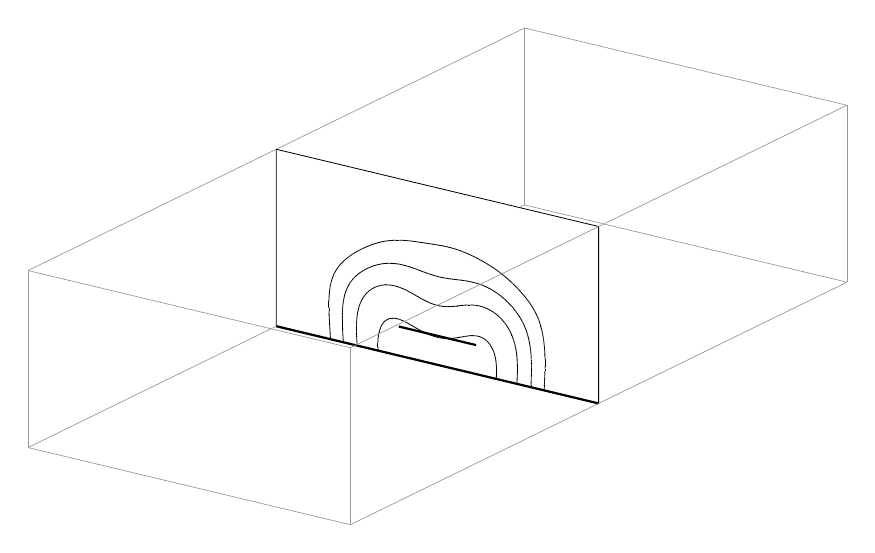
\begin{tikzpicture}
% generated by report/data/gen.py, do not edit
\draw[line width=0.25pt, black!40] (63.06mm,40.61mm) -- (63.06mm,63.08mm);
\draw[line width=0.25pt, black!40] (63.06mm,40.61mm) -- (104.00mm,30.80mm);
\draw[line width=0.25pt, black!40] (63.06mm,40.61mm) -- (31.53mm,25.21mm);
\draw[line width=0.25pt, black!40] (63.06mm,63.08mm) -- (104.00mm,53.27mm);
\draw[line width=0.25pt, black!40] (63.06mm,63.08mm) -- (31.53mm,47.68mm);
\draw[line width=0.25pt, black!40] (104.00mm,30.80mm) -- (104.00mm,53.27mm);
\draw[line width=0.25pt, black!40] (104.00mm,30.80mm) -- (72.47mm,15.40mm);
\draw[line width=0.25pt, black!40] (104.00mm,53.27mm) -- (72.47mm,37.87mm);
\filldraw[fill=white, draw=black, line width=0.30pt] (31.53mm,25.21mm) -- (72.47mm,15.40mm) -- (72.47mm,37.87mm) -- (31.53mm,47.68mm) -- cycle;
\draw[line width=0.30pt] (38.42mm,23.56mm) -- (38.40mm,23.81mm);
\draw[line width=0.30pt] (65.55mm,17.06mm) -- (65.56mm,17.31mm);
\draw[line width=0.30pt] (38.40mm,23.81mm) -- (38.38mm,24.07mm);
\draw[line width=0.30pt] (65.56mm,17.31mm) -- (65.57mm,17.48mm);
\draw[line width=0.30pt] (65.57mm,17.56mm) -- (65.57mm,17.48mm);
\draw[line width=0.30pt] (38.38mm,24.07mm) -- (38.37mm,24.33mm);
\draw[line width=0.30pt] (65.57mm,17.56mm) -- (65.58mm,17.81mm);
\draw[line width=0.30pt] (38.37mm,24.33mm) -- (38.35mm,24.58mm);
\draw[line width=0.30pt] (65.58mm,17.81mm) -- (65.59mm,18.06mm);
\draw[line width=0.30pt] (38.35mm,24.58mm) -- (38.34mm,24.84mm);
\draw[line width=0.30pt] (65.59mm,18.06mm) -- (65.60mm,18.31mm);
\draw[line width=0.30pt] (38.34mm,24.84mm) -- (38.32mm,25.09mm);
\draw[line width=0.30pt] (65.60mm,18.31mm) -- (65.61mm,18.56mm);
\draw[line width=0.30pt] (38.32mm,25.09mm) -- (38.31mm,25.35mm);
\draw[line width=0.30pt] (65.61mm,18.56mm) -- (65.62mm,18.81mm);
\draw[line width=0.30pt] (38.31mm,25.35mm) -- (38.29mm,25.61mm);
\draw[line width=0.30pt] (65.62mm,18.81mm) -- (65.63mm,19.06mm);
\draw[line width=0.30pt] (38.29mm,25.61mm) -- (38.28mm,25.86mm);
\draw[line width=0.30pt] (65.63mm,19.06mm) -- (65.64mm,19.31mm);
\draw[line width=0.30pt] (38.28mm,25.86mm) -- (38.26mm,26.12mm);
\draw[line width=0.30pt] (65.64mm,19.31mm) -- (65.65mm,19.56mm);
\draw[line width=0.30pt] (38.26mm,26.12mm) -- (38.25mm,26.37mm);
\draw[line width=0.30pt] (65.65mm,19.56mm) -- (65.65mm,19.81mm);
\draw[line width=0.30pt] (38.25mm,26.37mm) -- (38.24mm,26.63mm);
\draw[line width=0.30pt] (65.65mm,19.81mm) -- (65.66mm,20.06mm);
\draw[line width=0.30pt] (38.24mm,26.63mm) -- (38.23mm,26.88mm);
\draw[line width=0.30pt] (65.66mm,20.06mm) -- (65.66mm,20.31mm);
\draw[line width=0.30pt] (38.23mm,26.88mm) -- (38.22mm,27.14mm);
\draw[line width=0.30pt] (65.66mm,20.31mm) -- (65.66mm,20.57mm);
\draw[line width=0.30pt] (38.22mm,27.14mm) -- (38.22mm,27.39mm);
\draw[line width=0.30pt] (65.66mm,20.57mm) -- (65.66mm,20.82mm);
\draw[line width=0.30pt] (38.22mm,27.39mm) -- (38.21mm,27.65mm);
\draw[line width=0.30pt] (65.66mm,20.82mm) -- (65.66mm,21.07mm);
\draw[line width=0.30pt] (38.21mm,27.65mm) -- (38.21mm,27.90mm);
\draw[line width=0.30pt] (65.66mm,21.07mm) -- (65.65mm,21.33mm);
\draw[line width=0.30pt] (38.21mm,27.90mm) -- (38.21mm,28.15mm);
\draw[line width=0.30pt] (65.65mm,21.33mm) -- (65.64mm,21.58mm);
\draw[line width=0.30pt] (38.21mm,28.15mm) -- (38.21mm,28.40mm);
\draw[line width=0.30pt] (65.64mm,21.58mm) -- (65.63mm,21.84mm);
\draw[line width=0.30pt] (38.21mm,28.40mm) -- (38.22mm,28.65mm);
\draw[line width=0.30pt] (65.63mm,21.84mm) -- (65.62mm,22.09mm);
\draw[line width=0.30pt] (38.22mm,28.65mm) -- (38.23mm,28.90mm);
\draw[line width=0.30pt] (65.62mm,22.09mm) -- (65.60mm,22.35mm);
\draw[line width=0.30pt] (38.23mm,28.90mm) -- (38.25mm,29.15mm);
\draw[line width=0.30pt] (65.60mm,22.35mm) -- (65.58mm,22.61mm);
\draw[line width=0.30pt] (38.25mm,29.15mm) -- (38.27mm,29.40mm);
\draw[line width=0.30pt] (65.57mm,22.67mm) -- (65.55mm,22.87mm);
\draw[line width=0.30pt] (65.58mm,22.61mm) -- (65.57mm,22.67mm);
\draw[line width=0.30pt] (38.27mm,29.40mm) -- (38.29mm,29.65mm);
\draw[line width=0.30pt] (65.55mm,22.87mm) -- (65.52mm,23.12mm);
\draw[line width=0.30pt] (38.29mm,29.65mm) -- (38.32mm,29.89mm);
\draw[line width=0.30pt] (65.52mm,23.12mm) -- (65.49mm,23.39mm);
\draw[line width=0.30pt] (38.32mm,29.89mm) -- (38.36mm,30.14mm);
\draw[line width=0.30pt] (65.49mm,23.39mm) -- (65.45mm,23.65mm);
\draw[line width=0.30pt] (38.36mm,30.14mm) -- (38.40mm,30.38mm);
\draw[line width=0.30pt] (65.45mm,23.65mm) -- (65.41mm,23.91mm);
\draw[line width=0.30pt] (38.40mm,30.38mm) -- (38.43mm,30.53mm);
\draw[line width=0.30pt] (38.45mm,30.62mm) -- (38.43mm,30.53mm);
\draw[line width=0.30pt] (65.41mm,23.91mm) -- (65.36mm,24.17mm);
\draw[line width=0.30pt] (38.45mm,30.62mm) -- (38.51mm,30.86mm);
\draw[line width=0.30pt] (65.36mm,24.17mm) -- (65.31mm,24.44mm);
\draw[line width=0.30pt] (38.51mm,30.86mm) -- (38.58mm,31.09mm);
\draw[line width=0.30pt] (65.31mm,24.44mm) -- (65.25mm,24.70mm);
\draw[line width=0.30pt] (38.58mm,31.09mm) -- (38.65mm,31.33mm);
\draw[line width=0.30pt] (65.25mm,24.70mm) -- (65.18mm,24.97mm);
\draw[line width=0.30pt] (38.65mm,31.33mm) -- (38.74mm,31.56mm);
\draw[line width=0.30pt] (65.18mm,24.97mm) -- (65.11mm,25.24mm);
\draw[line width=0.30pt] (38.74mm,31.56mm) -- (38.84mm,31.79mm);
\draw[line width=0.30pt] (65.11mm,25.25mm) -- (65.03mm,25.52mm);
\draw[line width=0.30pt] (65.11mm,25.24mm) -- (65.11mm,25.25mm);
\draw[line width=0.30pt] (38.84mm,31.79mm) -- (38.89mm,31.90mm);
\draw[line width=0.30pt] (38.95mm,32.01mm) -- (38.89mm,31.90mm);
\draw[line width=0.30pt] (65.03mm,25.52mm) -- (64.94mm,25.79mm);
\draw[line width=0.30pt] (38.95mm,32.01mm) -- (39.07mm,32.24mm);
\draw[line width=0.30pt] (64.94mm,25.79mm) -- (64.84mm,26.07mm);
\draw[line width=0.30pt] (39.07mm,32.24mm) -- (39.21mm,32.46mm);
\draw[line width=0.30pt] (64.84mm,26.07mm) -- (64.73mm,26.35mm);
\draw[line width=0.30pt] (39.21mm,32.46mm) -- (39.35mm,32.66mm);
\draw[line width=0.30pt] (39.36mm,32.67mm) -- (39.35mm,32.66mm);
\draw[line width=0.30pt] (64.65mm,26.52mm) -- (64.60mm,26.63mm);
\draw[line width=0.30pt] (64.73mm,26.35mm) -- (64.65mm,26.52mm);
\draw[line width=0.30pt] (39.36mm,32.67mm) -- (39.52mm,32.89mm);
\draw[line width=0.30pt] (64.60mm,26.63mm) -- (64.46mm,26.91mm);
\draw[line width=0.30pt] (39.52mm,32.89mm) -- (39.70mm,33.10mm);
\draw[line width=0.30pt] (64.46mm,26.91mm) -- (64.31mm,27.20mm);
\draw[line width=0.30pt] (39.70mm,33.10mm) -- (39.81mm,33.21mm);
\draw[line width=0.30pt] (39.90mm,33.30mm) -- (39.81mm,33.21mm);
\draw[line width=0.30pt] (64.19mm,27.41mm) -- (64.14mm,27.50mm);
\draw[line width=0.30pt] (64.31mm,27.20mm) -- (64.19mm,27.41mm);
\draw[line width=0.30pt] (39.90mm,33.30mm) -- (40.11mm,33.50mm);
\draw[line width=0.30pt] (64.14mm,27.50mm) -- (63.96mm,27.79mm);
\draw[line width=0.30pt] (40.11mm,33.50mm) -- (40.27mm,33.65mm);
\draw[line width=0.30pt] (40.33mm,33.70mm) -- (40.27mm,33.65mm);
\draw[line width=0.30pt] (63.96mm,27.79mm) -- (63.76mm,28.09mm);
\draw[line width=0.30pt] (40.33mm,33.70mm) -- (40.57mm,33.90mm);
\draw[line width=0.30pt] (63.73mm,28.13mm) -- (63.54mm,28.40mm);
\draw[line width=0.30pt] (63.76mm,28.09mm) -- (63.73mm,28.13mm);
\draw[line width=0.30pt] (40.57mm,33.90mm) -- (40.73mm,34.02mm);
\draw[line width=0.30pt] (40.83mm,34.09mm) -- (40.73mm,34.02mm);
\draw[line width=0.30pt] (63.54mm,28.40mm) -- (63.30mm,28.71mm);
\draw[line width=0.30pt] (40.83mm,34.09mm) -- (41.10mm,34.28mm);
\draw[line width=0.30pt] (63.27mm,28.75mm) -- (63.05mm,29.02mm);
\draw[line width=0.30pt] (63.30mm,28.71mm) -- (63.27mm,28.75mm);
\draw[line width=0.30pt] (41.10mm,34.28mm) -- (41.19mm,34.34mm);
\draw[line width=0.30pt] (41.38mm,34.46mm) -- (41.19mm,34.34mm);
\draw[line width=0.30pt] (62.81mm,29.31mm) -- (62.79mm,29.33mm);
\draw[line width=0.30pt] (63.05mm,29.02mm) -- (62.81mm,29.31mm);
\draw[line width=0.30pt] (41.38mm,34.46mm) -- (41.65mm,34.62mm);
\draw[line width=0.30pt] (41.68mm,34.64mm) -- (41.65mm,34.62mm);
\draw[line width=0.30pt] (62.79mm,29.33mm) -- (62.50mm,29.66mm);
\draw[line width=0.30pt] (41.68mm,34.64mm) -- (42.00mm,34.82mm);
\draw[line width=0.30pt] (62.35mm,29.82mm) -- (62.20mm,29.98mm);
\draw[line width=0.30pt] (62.50mm,29.66mm) -- (62.35mm,29.82mm);
\draw[line width=0.30pt] (42.00mm,34.82mm) -- (42.11mm,34.88mm);
\draw[line width=0.30pt] (42.33mm,34.99mm) -- (42.11mm,34.88mm);
\draw[line width=0.30pt] (61.89mm,30.30mm) -- (61.88mm,30.31mm);
\draw[line width=0.30pt] (62.20mm,29.98mm) -- (61.89mm,30.30mm);
\draw[line width=0.30pt] (42.33mm,34.99mm) -- (42.57mm,35.11mm);
\draw[line width=0.30pt] (42.69mm,35.16mm) -- (42.57mm,35.11mm);
\draw[line width=0.30pt] (61.88mm,30.31mm) -- (61.54mm,30.64mm);
\draw[line width=0.30pt] (42.69mm,35.16mm) -- (43.03mm,35.31mm);
\draw[line width=0.30pt] (43.05mm,35.32mm) -- (43.03mm,35.31mm);
\draw[line width=0.30pt] (61.43mm,30.75mm) -- (61.18mm,30.98mm);
\draw[line width=0.30pt] (61.54mm,30.64mm) -- (61.43mm,30.75mm);
\draw[line width=0.30pt] (43.05mm,35.32mm) -- (43.45mm,35.48mm);
\draw[line width=0.30pt] (60.97mm,31.17mm) -- (60.79mm,31.33mm);
\draw[line width=0.30pt] (61.18mm,30.98mm) -- (60.97mm,31.17mm);
\draw[line width=0.30pt] (43.45mm,35.48mm) -- (43.49mm,35.50mm);
\draw[line width=0.30pt] (43.87mm,35.63mm) -- (43.49mm,35.50mm);
\draw[line width=0.30pt] (60.51mm,31.57mm) -- (60.37mm,31.68mm);
\draw[line width=0.30pt] (60.79mm,31.33mm) -- (60.51mm,31.57mm);
\draw[line width=0.30pt] (43.87mm,35.63mm) -- (43.95mm,35.66mm);
\draw[line width=0.30pt] (44.33mm,35.78mm) -- (43.95mm,35.66mm);
\draw[line width=0.30pt] (60.05mm,31.93mm) -- (59.90mm,32.05mm);
\draw[line width=0.30pt] (60.37mm,31.68mm) -- (60.05mm,31.93mm);
\draw[line width=0.30pt] (44.33mm,35.78mm) -- (44.41mm,35.80mm);
\draw[line width=0.30pt] (44.83mm,35.91mm) -- (44.41mm,35.80mm);
\draw[line width=0.30pt] (59.59mm,32.28mm) -- (59.38mm,32.42mm);
\draw[line width=0.30pt] (59.90mm,32.05mm) -- (59.59mm,32.28mm);
\draw[line width=0.30pt] (44.83mm,35.91mm) -- (44.87mm,35.92mm);
\draw[line width=0.30pt] (45.33mm,36.01mm) -- (44.87mm,35.92mm);
\draw[line width=0.30pt] (45.42mm,36.02mm) -- (45.33mm,36.01mm);
\draw[line width=0.30pt] (59.13mm,32.60mm) -- (58.80mm,32.81mm);
\draw[line width=0.30pt] (59.38mm,32.42mm) -- (59.13mm,32.60mm);
\draw[line width=0.30pt] (45.42mm,36.02mm) -- (45.79mm,36.07mm);
\draw[line width=0.30pt] (46.13mm,36.10mm) -- (45.79mm,36.07mm);
\draw[line width=0.30pt] (58.21mm,33.18mm) -- (58.14mm,33.23mm);
\draw[line width=0.30pt] (58.67mm,32.90mm) -- (58.21mm,33.18mm);
\draw[line width=0.30pt] (58.80mm,32.81mm) -- (58.67mm,32.90mm);
\draw[line width=0.30pt] (46.13mm,36.10mm) -- (46.25mm,36.11mm);
\draw[line width=0.30pt] (46.71mm,36.13mm) -- (46.25mm,36.11mm);
\draw[line width=0.30pt] (47.05mm,36.13mm) -- (46.71mm,36.13mm);
\draw[line width=0.30pt] (57.75mm,33.45mm) -- (57.36mm,33.66mm);
\draw[line width=0.30pt] (58.14mm,33.23mm) -- (57.75mm,33.45mm);
\draw[line width=0.30pt] (47.05mm,36.13mm) -- (47.17mm,36.13mm);
\draw[line width=0.30pt] (47.63mm,36.12mm) -- (47.17mm,36.13mm);
\draw[line width=0.30pt] (48.09mm,36.08mm) -- (47.63mm,36.12mm);
\draw[line width=0.30pt] (48.47mm,36.05mm) -- (48.09mm,36.08mm);
\draw[line width=0.30pt] (56.83mm,33.95mm) -- (56.44mm,34.14mm);
\draw[line width=0.30pt] (57.29mm,33.70mm) -- (56.83mm,33.95mm);
\draw[line width=0.30pt] (57.36mm,33.66mm) -- (57.29mm,33.70mm);
\draw[line width=0.30pt] (48.47mm,36.05mm) -- (48.55mm,36.04mm);
\draw[line width=0.30pt] (49.01mm,35.98mm) -- (48.55mm,36.04mm);
\draw[line width=0.30pt] (49.47mm,35.92mm) -- (49.01mm,35.98mm);
\draw[line width=0.30pt] (49.93mm,35.85mm) -- (49.47mm,35.92mm);
\draw[line width=0.30pt] (50.39mm,35.78mm) -- (49.93mm,35.85mm);
\draw[line width=0.30pt] (50.85mm,35.71mm) -- (50.39mm,35.78mm);
\draw[line width=0.30pt] (51.05mm,35.68mm) -- (50.85mm,35.71mm);
\draw[line width=0.30pt] (55.45mm,34.58mm) -- (55.17mm,34.69mm);
\draw[line width=0.30pt] (55.91mm,34.39mm) -- (55.45mm,34.58mm);
\draw[line width=0.30pt] (56.37mm,34.17mm) -- (55.91mm,34.39mm);
\draw[line width=0.30pt] (56.44mm,34.14mm) -- (56.37mm,34.17mm);
\draw[line width=0.30pt] (51.05mm,35.68mm) -- (51.31mm,35.64mm);
\draw[line width=0.30pt] (51.77mm,35.57mm) -- (51.31mm,35.64mm);
\draw[line width=0.30pt] (52.23mm,35.49mm) -- (51.77mm,35.57mm);
\draw[line width=0.30pt] (52.69mm,35.41mm) -- (52.23mm,35.49mm);
\draw[line width=0.30pt] (53.15mm,35.31mm) -- (52.69mm,35.41mm);
\draw[line width=0.30pt] (53.61mm,35.20mm) -- (53.15mm,35.31mm);
\draw[line width=0.30pt] (54.07mm,35.07mm) -- (53.61mm,35.20mm);
\draw[line width=0.30pt] (54.53mm,34.93mm) -- (54.07mm,35.07mm);
\draw[line width=0.30pt] (54.99mm,34.77mm) -- (54.53mm,34.93mm);
\draw[line width=0.30pt] (55.17mm,34.69mm) -- (54.99mm,34.77mm);
\draw[line width=0.30pt] (40.04mm,23.17mm) -- (40.03mm,23.42mm);
\draw[line width=0.30pt] (63.88mm,17.46mm) -- (63.88mm,17.71mm);
\draw[line width=0.30pt] (40.03mm,23.42mm) -- (40.01mm,23.68mm);
\draw[line width=0.30pt] (63.88mm,17.71mm) -- (63.89mm,17.96mm);
\draw[line width=0.30pt] (40.01mm,23.68mm) -- (40.00mm,23.94mm);
\draw[line width=0.30pt] (63.89mm,17.96mm) -- (63.90mm,18.21mm);
\draw[line width=0.30pt] (40.00mm,23.94mm) -- (39.98mm,24.19mm);
\draw[line width=0.30pt] (63.90mm,18.21mm) -- (63.91mm,18.46mm);
\draw[line width=0.30pt] (39.98mm,24.19mm) -- (39.97mm,24.45mm);
\draw[line width=0.30pt] (63.91mm,18.46mm) -- (63.92mm,18.71mm);
\draw[line width=0.30pt] (39.97mm,24.45mm) -- (39.96mm,24.70mm);
\draw[line width=0.30pt] (63.92mm,18.71mm) -- (63.92mm,18.96mm);
\draw[line width=0.30pt] (39.96mm,24.70mm) -- (39.95mm,24.96mm);
\draw[line width=0.30pt] (63.92mm,18.96mm) -- (63.93mm,19.21mm);
\draw[line width=0.30pt] (39.95mm,24.96mm) -- (39.94mm,25.21mm);
\draw[line width=0.30pt] (63.93mm,19.21mm) -- (63.93mm,19.47mm);
\draw[line width=0.30pt] (39.94mm,25.21mm) -- (39.93mm,25.47mm);
\draw[line width=0.30pt] (63.93mm,19.47mm) -- (63.93mm,19.72mm);
\draw[line width=0.30pt] (39.93mm,25.47mm) -- (39.92mm,25.72mm);
\draw[line width=0.30pt] (63.93mm,19.72mm) -- (63.94mm,19.97mm);
\draw[line width=0.30pt] (39.92mm,25.72mm) -- (39.92mm,25.97mm);
\draw[line width=0.30pt] (63.94mm,19.97mm) -- (63.93mm,20.22mm);
\draw[line width=0.30pt] (39.92mm,25.97mm) -- (39.91mm,26.23mm);
\draw[line width=0.30pt] (63.93mm,20.22mm) -- (63.93mm,20.48mm);
\draw[line width=0.30pt] (39.91mm,26.23mm) -- (39.91mm,26.48mm);
\draw[line width=0.30pt] (63.93mm,20.48mm) -- (63.92mm,20.73mm);
\draw[line width=0.30pt] (39.91mm,26.48mm) -- (39.92mm,26.73mm);
\draw[line width=0.30pt] (63.92mm,20.73mm) -- (63.92mm,20.98mm);
\draw[line width=0.30pt] (39.92mm,26.73mm) -- (39.93mm,26.98mm);
\draw[line width=0.30pt] (63.92mm,20.98mm) -- (63.90mm,21.24mm);
\draw[line width=0.30pt] (39.93mm,26.98mm) -- (39.94mm,27.23mm);
\draw[line width=0.30pt] (63.90mm,21.24mm) -- (63.89mm,21.50mm);
\draw[line width=0.30pt] (39.94mm,27.23mm) -- (39.95mm,27.48mm);
\draw[line width=0.30pt] (63.89mm,21.50mm) -- (63.87mm,21.75mm);
\draw[line width=0.30pt] (39.95mm,27.48mm) -- (39.97mm,27.73mm);
\draw[line width=0.30pt] (63.87mm,21.75mm) -- (63.84mm,22.01mm);
\draw[line width=0.30pt] (39.97mm,27.73mm) -- (40.00mm,27.98mm);
\draw[line width=0.30pt] (63.84mm,22.01mm) -- (63.81mm,22.27mm);
\draw[line width=0.30pt] (40.00mm,27.98mm) -- (40.03mm,28.22mm);
\draw[line width=0.30pt] (63.81mm,22.27mm) -- (63.78mm,22.53mm);
\draw[line width=0.30pt] (40.03mm,28.22mm) -- (40.06mm,28.46mm);
\draw[line width=0.30pt] (63.78mm,22.53mm) -- (63.74mm,22.79mm);
\draw[line width=0.30pt] (40.06mm,28.46mm) -- (40.11mm,28.71mm);
\draw[line width=0.30pt] (63.73mm,22.85mm) -- (63.69mm,23.06mm);
\draw[line width=0.30pt] (63.74mm,22.79mm) -- (63.73mm,22.85mm);
\draw[line width=0.30pt] (40.11mm,28.71mm) -- (40.16mm,28.95mm);
\draw[line width=0.30pt] (63.69mm,23.06mm) -- (63.64mm,23.32mm);
\draw[line width=0.30pt] (40.16mm,28.95mm) -- (40.22mm,29.18mm);
\draw[line width=0.30pt] (63.64mm,23.32mm) -- (63.58mm,23.59mm);
\draw[line width=0.30pt] (40.22mm,29.18mm) -- (40.27mm,29.37mm);
\draw[line width=0.30pt] (40.29mm,29.42mm) -- (40.27mm,29.37mm);
\draw[line width=0.30pt] (63.58mm,23.59mm) -- (63.51mm,23.86mm);
\draw[line width=0.30pt] (40.29mm,29.42mm) -- (40.37mm,29.65mm);
\draw[line width=0.30pt] (63.51mm,23.86mm) -- (63.44mm,24.13mm);
\draw[line width=0.30pt] (40.37mm,29.65mm) -- (40.46mm,29.89mm);
\draw[line width=0.30pt] (63.44mm,24.13mm) -- (63.35mm,24.40mm);
\draw[line width=0.30pt] (40.46mm,29.89mm) -- (40.56mm,30.11mm);
\draw[line width=0.30pt] (63.27mm,24.65mm) -- (63.26mm,24.68mm);
\draw[line width=0.30pt] (63.35mm,24.40mm) -- (63.27mm,24.65mm);
\draw[line width=0.30pt] (40.56mm,30.11mm) -- (40.67mm,30.34mm);
\draw[line width=0.30pt] (63.26mm,24.68mm) -- (63.16mm,24.95mm);
\draw[line width=0.30pt] (40.67mm,30.34mm) -- (40.73mm,30.45mm);
\draw[line width=0.30pt] (40.80mm,30.56mm) -- (40.73mm,30.45mm);
\draw[line width=0.30pt] (63.16mm,24.95mm) -- (63.04mm,25.23mm);
\draw[line width=0.30pt] (40.80mm,30.56mm) -- (40.94mm,30.78mm);
\draw[line width=0.30pt] (63.04mm,25.23mm) -- (62.91mm,25.52mm);
\draw[line width=0.30pt] (40.94mm,30.78mm) -- (41.10mm,30.99mm);
\draw[line width=0.30pt] (62.81mm,25.72mm) -- (62.77mm,25.80mm);
\draw[line width=0.30pt] (62.91mm,25.52mm) -- (62.81mm,25.72mm);
\draw[line width=0.30pt] (41.10mm,30.99mm) -- (41.19mm,31.11mm);
\draw[line width=0.30pt] (41.27mm,31.21mm) -- (41.19mm,31.11mm);
\draw[line width=0.30pt] (62.77mm,25.80mm) -- (62.61mm,26.10mm);
\draw[line width=0.30pt] (41.27mm,31.21mm) -- (41.46mm,31.41mm);
\draw[line width=0.30pt] (62.61mm,26.10mm) -- (62.43mm,26.39mm);
\draw[line width=0.30pt] (41.46mm,31.41mm) -- (41.65mm,31.59mm);
\draw[line width=0.30pt] (41.67mm,31.61mm) -- (41.65mm,31.59mm);
\draw[line width=0.30pt] (62.35mm,26.52mm) -- (62.24mm,26.69mm);
\draw[line width=0.30pt] (62.43mm,26.39mm) -- (62.35mm,26.52mm);
\draw[line width=0.30pt] (41.67mm,31.61mm) -- (41.91mm,31.81mm);
\draw[line width=0.30pt] (62.24mm,26.69mm) -- (62.02mm,26.99mm);
\draw[line width=0.30pt] (41.91mm,31.81mm) -- (42.11mm,31.97mm);
\draw[line width=0.30pt] (42.16mm,32.00mm) -- (42.11mm,31.97mm);
\draw[line width=0.30pt] (61.89mm,27.17mm) -- (61.79mm,27.30mm);
\draw[line width=0.30pt] (62.02mm,26.99mm) -- (61.89mm,27.17mm);
\draw[line width=0.30pt] (42.16mm,32.00mm) -- (42.43mm,32.19mm);
\draw[line width=0.30pt] (61.79mm,27.30mm) -- (61.53mm,27.62mm);
\draw[line width=0.30pt] (42.43mm,32.19mm) -- (42.57mm,32.28mm);
\draw[line width=0.30pt] (42.74mm,32.37mm) -- (42.57mm,32.28mm);
\draw[line width=0.30pt] (61.43mm,27.73mm) -- (61.24mm,27.94mm);
\draw[line width=0.30pt] (61.53mm,27.62mm) -- (61.43mm,27.73mm);
\draw[line width=0.30pt] (42.74mm,32.37mm) -- (43.03mm,32.53mm);
\draw[line width=0.30pt] (43.07mm,32.54mm) -- (43.03mm,32.53mm);
\draw[line width=0.30pt] (60.97mm,28.22mm) -- (60.92mm,28.27mm);
\draw[line width=0.30pt] (61.24mm,27.94mm) -- (60.97mm,28.22mm);
\draw[line width=0.30pt] (43.07mm,32.54mm) -- (43.43mm,32.71mm);
\draw[line width=0.30pt] (60.92mm,28.27mm) -- (60.57mm,28.60mm);
\draw[line width=0.30pt] (43.43mm,32.71mm) -- (43.49mm,32.73mm);
\draw[line width=0.30pt] (43.85mm,32.86mm) -- (43.49mm,32.73mm);
\draw[line width=0.30pt] (60.51mm,28.66mm) -- (60.16mm,28.95mm);
\draw[line width=0.30pt] (60.57mm,28.60mm) -- (60.51mm,28.66mm);
\draw[line width=0.30pt] (43.85mm,32.86mm) -- (43.95mm,32.90mm);
\draw[line width=0.30pt] (44.32mm,33.00mm) -- (43.95mm,32.90mm);
\draw[line width=0.30pt] (60.05mm,29.05mm) -- (59.69mm,29.32mm);
\draw[line width=0.30pt] (60.16mm,28.95mm) -- (60.05mm,29.05mm);
\draw[line width=0.30pt] (44.32mm,33.00mm) -- (44.41mm,33.03mm);
\draw[line width=0.30pt] (44.87mm,33.12mm) -- (44.41mm,33.03mm);
\draw[line width=0.30pt] (44.87mm,33.12mm) -- (44.87mm,33.12mm);
\draw[line width=0.30pt] (59.13mm,29.70mm) -- (59.11mm,29.71mm);
\draw[line width=0.30pt] (59.59mm,29.39mm) -- (59.13mm,29.70mm);
\draw[line width=0.30pt] (59.69mm,29.32mm) -- (59.59mm,29.39mm);
\draw[line width=0.30pt] (44.87mm,33.12mm) -- (45.33mm,33.18mm);
\draw[line width=0.30pt] (45.62mm,33.19mm) -- (45.33mm,33.18mm);
\draw[line width=0.30pt] (50.39mm,32.05mm) -- (50.38mm,32.05mm);
\draw[line width=0.30pt] (50.85mm,31.88mm) -- (50.39mm,32.05mm);
\draw[line width=0.30pt] (51.31mm,31.73mm) -- (50.85mm,31.88mm);
\draw[line width=0.30pt] (51.77mm,31.59mm) -- (51.31mm,31.73mm);
\draw[line width=0.30pt] (52.23mm,31.47mm) -- (51.77mm,31.59mm);
\draw[line width=0.30pt] (52.69mm,31.37mm) -- (52.23mm,31.47mm);
\draw[line width=0.30pt] (53.15mm,31.29mm) -- (52.69mm,31.37mm);
\draw[line width=0.30pt] (53.61mm,31.22mm) -- (53.15mm,31.29mm);
\draw[line width=0.30pt] (54.07mm,31.17mm) -- (53.61mm,31.22mm);
\draw[line width=0.30pt] (54.08mm,31.17mm) -- (54.07mm,31.17mm);
\draw[line width=0.30pt] (58.67mm,29.96mm) -- (58.28mm,30.16mm);
\draw[line width=0.30pt] (59.11mm,29.71mm) -- (58.67mm,29.96mm);
\draw[line width=0.30pt] (45.62mm,33.19mm) -- (45.79mm,33.20mm);
\draw[line width=0.30pt] (46.25mm,33.19mm) -- (45.79mm,33.20mm);
\draw[line width=0.30pt] (46.71mm,33.15mm) -- (46.25mm,33.19mm);
\draw[line width=0.30pt] (47.08mm,33.10mm) -- (46.71mm,33.15mm);
\draw[line width=0.30pt] (48.55mm,32.72mm) -- (48.22mm,32.82mm);
\draw[line width=0.30pt] (49.01mm,32.56mm) -- (48.55mm,32.72mm);
\draw[line width=0.30pt] (49.47mm,32.40mm) -- (49.01mm,32.56mm);
\draw[line width=0.30pt] (49.93mm,32.22mm) -- (49.47mm,32.40mm);
\draw[line width=0.30pt] (50.38mm,32.05mm) -- (49.93mm,32.22mm);
\draw[line width=0.30pt] (54.08mm,31.17mm) -- (54.53mm,31.11mm);
\draw[line width=0.30pt] (54.99mm,31.06mm) -- (54.53mm,31.11mm);
\draw[line width=0.30pt] (55.45mm,30.99mm) -- (54.99mm,31.06mm);
\draw[line width=0.30pt] (55.91mm,30.92mm) -- (55.45mm,30.99mm);
\draw[line width=0.30pt] (56.37mm,30.82mm) -- (55.91mm,30.92mm);
\draw[line width=0.30pt] (56.83mm,30.70mm) -- (56.37mm,30.82mm);
\draw[line width=0.30pt] (57.29mm,30.56mm) -- (56.83mm,30.70mm);
\draw[line width=0.30pt] (57.75mm,30.39mm) -- (57.29mm,30.56mm);
\draw[line width=0.30pt] (58.21mm,30.20mm) -- (57.75mm,30.39mm);
\draw[line width=0.30pt] (58.28mm,30.16mm) -- (58.21mm,30.20mm);
\draw[line width=0.30pt] (47.08mm,33.10mm) -- (47.17mm,33.08mm);
\draw[line width=0.30pt] (47.63mm,32.98mm) -- (47.17mm,33.08mm);
\draw[line width=0.30pt] (48.09mm,32.86mm) -- (47.63mm,32.98mm);
\draw[line width=0.30pt] (48.22mm,32.82mm) -- (48.09mm,32.86mm);
\draw[line width=0.30pt] (41.80mm,22.75mm) -- (41.78mm,23.00mm);
\draw[line width=0.30pt] (62.09mm,17.89mm) -- (62.10mm,18.14mm);
\draw[line width=0.30pt] (41.78mm,23.00mm) -- (41.77mm,23.26mm);
\draw[line width=0.30pt] (62.10mm,18.14mm) -- (62.11mm,18.39mm);
\draw[line width=0.30pt] (41.77mm,23.26mm) -- (41.75mm,23.51mm);
\draw[line width=0.30pt] (62.11mm,18.39mm) -- (62.12mm,18.64mm);
\draw[line width=0.30pt] (41.75mm,23.51mm) -- (41.74mm,23.77mm);
\draw[line width=0.30pt] (62.12mm,18.64mm) -- (62.13mm,18.89mm);
\draw[line width=0.30pt] (41.74mm,23.77mm) -- (41.73mm,24.03mm);
\draw[line width=0.30pt] (62.13mm,18.89mm) -- (62.14mm,19.14mm);
\draw[line width=0.30pt] (41.73mm,24.03mm) -- (41.72mm,24.28mm);
\draw[line width=0.30pt] (62.14mm,19.14mm) -- (62.14mm,19.39mm);
\draw[line width=0.30pt] (41.72mm,24.28mm) -- (41.72mm,24.53mm);
\draw[line width=0.30pt] (62.14mm,19.39mm) -- (62.15mm,19.64mm);
\draw[line width=0.30pt] (41.72mm,24.53mm) -- (41.71mm,24.79mm);
\draw[line width=0.30pt] (62.15mm,19.64mm) -- (62.15mm,19.89mm);
\draw[line width=0.30pt] (41.71mm,24.79mm) -- (41.71mm,25.04mm);
\draw[line width=0.30pt] (62.15mm,19.89mm) -- (62.15mm,20.15mm);
\draw[line width=0.30pt] (41.71mm,25.04mm) -- (41.71mm,25.29mm);
\draw[line width=0.30pt] (62.15mm,20.15mm) -- (62.14mm,20.40mm);
\draw[line width=0.30pt] (41.71mm,25.29mm) -- (41.72mm,25.54mm);
\draw[line width=0.30pt] (62.14mm,20.40mm) -- (62.13mm,20.65mm);
\draw[line width=0.30pt] (41.72mm,25.54mm) -- (41.73mm,25.79mm);
\draw[line width=0.30pt] (62.13mm,20.65mm) -- (62.12mm,20.91mm);
\draw[line width=0.30pt] (41.73mm,25.79mm) -- (41.75mm,26.04mm);
\draw[line width=0.30pt] (62.12mm,20.91mm) -- (62.10mm,21.17mm);
\draw[line width=0.30pt] (41.75mm,26.04mm) -- (41.77mm,26.29mm);
\draw[line width=0.30pt] (62.10mm,21.17mm) -- (62.08mm,21.43mm);
\draw[line width=0.30pt] (41.77mm,26.29mm) -- (41.80mm,26.53mm);
\draw[line width=0.30pt] (62.08mm,21.43mm) -- (62.05mm,21.68mm);
\draw[line width=0.30pt] (41.80mm,26.53mm) -- (41.84mm,26.78mm);
\draw[line width=0.30pt] (62.05mm,21.68mm) -- (62.01mm,21.95mm);
\draw[line width=0.30pt] (41.84mm,26.78mm) -- (41.88mm,27.02mm);
\draw[line width=0.30pt] (62.01mm,21.95mm) -- (61.97mm,22.21mm);
\draw[line width=0.30pt] (41.88mm,27.02mm) -- (41.93mm,27.26mm);
\draw[line width=0.30pt] (61.97mm,22.21mm) -- (61.92mm,22.47mm);
\draw[line width=0.30pt] (41.93mm,27.26mm) -- (41.99mm,27.50mm);
\draw[line width=0.30pt] (61.89mm,22.64mm) -- (61.87mm,22.74mm);
\draw[line width=0.30pt] (61.92mm,22.47mm) -- (61.89mm,22.64mm);
\draw[line width=0.30pt] (41.99mm,27.50mm) -- (42.05mm,27.74mm);
\draw[line width=0.30pt] (61.87mm,22.74mm) -- (61.80mm,23.01mm);
\draw[line width=0.30pt] (42.05mm,27.74mm) -- (42.11mm,27.91mm);
\draw[line width=0.30pt] (42.13mm,27.97mm) -- (42.11mm,27.91mm);
\draw[line width=0.30pt] (61.80mm,23.01mm) -- (61.72mm,23.28mm);
\draw[line width=0.30pt] (42.13mm,27.97mm) -- (42.23mm,28.20mm);
\draw[line width=0.30pt] (61.72mm,23.28mm) -- (61.63mm,23.55mm);
\draw[line width=0.30pt] (42.23mm,28.20mm) -- (42.33mm,28.43mm);
\draw[line width=0.30pt] (61.63mm,23.55mm) -- (61.53mm,23.83mm);
\draw[line width=0.30pt] (42.33mm,28.43mm) -- (42.45mm,28.65mm);
\draw[line width=0.30pt] (61.43mm,24.10mm) -- (61.43mm,24.11mm);
\draw[line width=0.30pt] (61.53mm,23.83mm) -- (61.43mm,24.10mm);
\draw[line width=0.30pt] (42.45mm,28.65mm) -- (42.57mm,28.86mm);
\draw[line width=0.30pt] (42.58mm,28.87mm) -- (42.57mm,28.86mm);
\draw[line width=0.30pt] (61.43mm,24.11mm) -- (61.29mm,24.39mm);
\draw[line width=0.30pt] (42.58mm,28.87mm) -- (42.73mm,29.09mm);
\draw[line width=0.30pt] (61.29mm,24.39mm) -- (61.15mm,24.68mm);
\draw[line width=0.30pt] (42.73mm,29.09mm) -- (42.91mm,29.30mm);
\draw[line width=0.30pt] (61.15mm,24.68mm) -- (60.99mm,24.97mm);
\draw[line width=0.30pt] (42.91mm,29.30mm) -- (43.03mm,29.44mm);
\draw[line width=0.30pt] (43.10mm,29.50mm) -- (43.03mm,29.44mm);
\draw[line width=0.30pt] (60.97mm,25.00mm) -- (60.80mm,25.27mm);
\draw[line width=0.30pt] (60.99mm,24.97mm) -- (60.97mm,25.00mm);
\draw[line width=0.30pt] (43.10mm,29.50mm) -- (43.33mm,29.70mm);
\draw[line width=0.30pt] (60.80mm,25.27mm) -- (60.59mm,25.57mm);
\draw[line width=0.30pt] (43.33mm,29.70mm) -- (43.49mm,29.83mm);
\draw[line width=0.30pt] (43.59mm,29.89mm) -- (43.49mm,29.83mm);
\draw[line width=0.30pt] (51.77mm,27.91mm) -- (51.53mm,27.99mm);
\draw[line width=0.30pt] (52.23mm,27.80mm) -- (51.77mm,27.91mm);
\draw[line width=0.30pt] (52.51mm,27.76mm) -- (52.23mm,27.80mm);
\draw[line width=0.30pt] (60.51mm,25.67mm) -- (60.33mm,25.88mm);
\draw[line width=0.30pt] (60.59mm,25.57mm) -- (60.51mm,25.67mm);
\draw[line width=0.30pt] (43.59mm,29.89mm) -- (43.89mm,30.07mm);
\draw[line width=0.30pt] (50.39mm,28.48mm) -- (50.26mm,28.55mm);
\draw[line width=0.30pt] (50.85mm,28.25mm) -- (50.39mm,28.48mm);
\draw[line width=0.30pt] (51.31mm,28.06mm) -- (50.85mm,28.25mm);
\draw[line width=0.30pt] (51.53mm,27.99mm) -- (51.31mm,28.06mm);
\draw[line width=0.30pt] (52.51mm,27.76mm) -- (52.69mm,27.73mm);
\draw[line width=0.30pt] (53.15mm,27.70mm) -- (52.69mm,27.73mm);
\draw[line width=0.30pt] (53.61mm,27.70mm) -- (53.15mm,27.70mm);
\draw[line width=0.30pt] (53.75mm,27.71mm) -- (53.61mm,27.70mm);
\draw[line width=0.30pt] (60.33mm,25.88mm) -- (60.05mm,26.20mm);
\draw[line width=0.30pt] (43.89mm,30.07mm) -- (43.95mm,30.11mm);
\draw[line width=0.30pt] (44.27mm,30.24mm) -- (43.95mm,30.11mm);
\draw[line width=0.30pt] (49.47mm,28.99mm) -- (49.46mm,28.99mm);
\draw[line width=0.30pt] (49.93mm,28.72mm) -- (49.47mm,28.99mm);
\draw[line width=0.30pt] (50.26mm,28.55mm) -- (49.93mm,28.72mm);
\draw[line width=0.30pt] (53.75mm,27.71mm) -- (54.07mm,27.73mm);
\draw[line width=0.30pt] (54.51mm,27.78mm) -- (54.07mm,27.73mm);
\draw[line width=0.30pt] (60.05mm,26.20mm) -- (59.69mm,26.54mm);
\draw[line width=0.30pt] (60.05mm,26.20mm) -- (60.05mm,26.20mm);
\draw[line width=0.30pt] (44.27mm,30.24mm) -- (44.41mm,30.29mm);
\draw[line width=0.30pt] (44.74mm,30.37mm) -- (44.41mm,30.29mm);
\draw[line width=0.30pt] (49.01mm,29.25mm) -- (48.71mm,29.42mm);
\draw[line width=0.30pt] (49.46mm,28.99mm) -- (49.01mm,29.25mm);
\draw[line width=0.30pt] (54.51mm,27.78mm) -- (54.53mm,27.78mm);
\draw[line width=0.30pt] (54.99mm,27.84mm) -- (54.53mm,27.78mm);
\draw[line width=0.30pt] (55.23mm,27.86mm) -- (54.99mm,27.84mm);
\draw[line width=0.30pt] (59.59mm,26.63mm) -- (59.24mm,26.90mm);
\draw[line width=0.30pt] (59.69mm,26.54mm) -- (59.59mm,26.63mm);
\draw[line width=0.30pt] (44.74mm,30.37mm) -- (44.87mm,30.41mm);
\draw[line width=0.30pt] (45.33mm,30.46mm) -- (44.87mm,30.41mm);
\draw[line width=0.30pt] (45.45mm,30.46mm) -- (45.33mm,30.46mm);
\draw[line width=0.30pt] (48.09mm,29.75mm) -- (47.79mm,29.90mm);
\draw[line width=0.30pt] (48.55mm,29.51mm) -- (48.09mm,29.75mm);
\draw[line width=0.30pt] (48.71mm,29.42mm) -- (48.55mm,29.51mm);
\draw[line width=0.30pt] (55.23mm,27.86mm) -- (55.45mm,27.88mm);
\draw[line width=0.30pt] (55.91mm,27.91mm) -- (55.45mm,27.88mm);
\draw[line width=0.30pt] (56.10mm,27.91mm) -- (55.91mm,27.91mm);
\draw[line width=0.30pt] (58.67mm,27.27mm) -- (58.57mm,27.31mm);
\draw[line width=0.30pt] (59.13mm,26.98mm) -- (58.67mm,27.27mm);
\draw[line width=0.30pt] (59.24mm,26.90mm) -- (59.13mm,26.98mm);
\draw[line width=0.30pt] (45.45mm,30.46mm) -- (45.79mm,30.45mm);
\draw[line width=0.30pt] (46.25mm,30.40mm) -- (45.79mm,30.45mm);
\draw[line width=0.30pt] (46.71mm,30.30mm) -- (46.25mm,30.40mm);
\draw[line width=0.30pt] (47.17mm,30.15mm) -- (46.71mm,30.30mm);
\draw[line width=0.30pt] (47.63mm,29.97mm) -- (47.17mm,30.15mm);
\draw[line width=0.30pt] (47.79mm,29.90mm) -- (47.63mm,29.97mm);
\draw[line width=0.30pt] (56.10mm,27.91mm) -- (56.37mm,27.90mm);
\draw[line width=0.30pt] (56.83mm,27.87mm) -- (56.37mm,27.90mm);
\draw[line width=0.30pt] (57.29mm,27.79mm) -- (56.83mm,27.87mm);
\draw[line width=0.30pt] (57.75mm,27.66mm) -- (57.29mm,27.79mm);
\draw[line width=0.30pt] (58.21mm,27.49mm) -- (57.75mm,27.66mm);
\draw[line width=0.30pt] (58.57mm,27.31mm) -- (58.21mm,27.49mm);
\draw[line width=0.30pt] (44.44mm,22.11mm) -- (44.44mm,22.37mm);
\draw[line width=0.30pt] (59.46mm,18.52mm) -- (59.48mm,18.77mm);
\draw[line width=0.30pt] (44.44mm,22.37mm) -- (44.43mm,22.62mm);
\draw[line width=0.30pt] (59.48mm,18.77mm) -- (59.49mm,19.02mm);
\draw[line width=0.30pt] (44.43mm,22.62mm) -- (44.43mm,22.87mm);
\draw[line width=0.30pt] (59.49mm,19.02mm) -- (59.50mm,19.27mm);
\draw[line width=0.30pt] (44.43mm,22.87mm) -- (44.43mm,23.13mm);
\draw[line width=0.30pt] (59.50mm,19.27mm) -- (59.50mm,19.52mm);
\draw[line width=0.30pt] (44.43mm,23.13mm) -- (44.44mm,23.38mm);
\draw[line width=0.30pt] (59.50mm,19.52mm) -- (59.50mm,19.77mm);
\draw[line width=0.30pt] (44.44mm,23.38mm) -- (44.46mm,23.62mm);
\draw[line width=0.30pt] (59.50mm,19.77mm) -- (59.49mm,20.02mm);
\draw[line width=0.30pt] (44.46mm,23.62mm) -- (44.49mm,23.87mm);
\draw[line width=0.30pt] (59.49mm,20.02mm) -- (59.47mm,20.28mm);
\draw[line width=0.30pt] (44.49mm,23.87mm) -- (44.52mm,24.11mm);
\draw[line width=0.30pt] (59.47mm,20.28mm) -- (59.45mm,20.54mm);
\draw[line width=0.30pt] (44.52mm,24.11mm) -- (44.57mm,24.36mm);
\draw[line width=0.30pt] (59.45mm,20.54mm) -- (59.42mm,20.80mm);
\draw[line width=0.30pt] (44.57mm,24.36mm) -- (44.63mm,24.59mm);
\draw[line width=0.30pt] (59.42mm,20.80mm) -- (59.38mm,21.06mm);
\draw[line width=0.30pt] (44.63mm,24.59mm) -- (44.70mm,24.83mm);
\draw[line width=0.30pt] (59.38mm,21.06mm) -- (59.32mm,21.33mm);
\draw[line width=0.30pt] (44.70mm,24.83mm) -- (44.78mm,25.06mm);
\draw[line width=0.30pt] (59.32mm,21.33mm) -- (59.26mm,21.60mm);
\draw[line width=0.30pt] (44.78mm,25.06mm) -- (44.87mm,25.27mm);
\draw[line width=0.30pt] (44.88mm,25.29mm) -- (44.87mm,25.27mm);
\draw[line width=0.30pt] (59.26mm,21.60mm) -- (59.18mm,21.87mm);
\draw[line width=0.30pt] (44.88mm,25.29mm) -- (45.03mm,25.51mm);
\draw[line width=0.30pt] (51.31mm,24.00mm) -- (51.30mm,24.01mm);
\draw[line width=0.30pt] (51.77mm,23.86mm) -- (51.31mm,24.00mm);
\draw[line width=0.30pt] (52.23mm,23.75mm) -- (51.77mm,23.86mm);
\draw[line width=0.30pt] (52.56mm,23.70mm) -- (52.23mm,23.75mm);
\draw[line width=0.30pt] (59.13mm,22.01mm) -- (59.07mm,22.14mm);
\draw[line width=0.30pt] (59.18mm,21.87mm) -- (59.13mm,22.01mm);
\draw[line width=0.30pt] (45.03mm,25.51mm) -- (45.19mm,25.72mm);
\draw[line width=0.30pt] (50.39mm,24.38mm) -- (50.03mm,24.56mm);
\draw[line width=0.30pt] (50.85mm,24.18mm) -- (50.39mm,24.38mm);
\draw[line width=0.30pt] (51.30mm,24.01mm) -- (50.85mm,24.18mm);
\draw[line width=0.30pt] (52.56mm,23.70mm) -- (52.69mm,23.68mm);
\draw[line width=0.30pt] (53.15mm,23.65mm) -- (52.69mm,23.68mm);
\draw[line width=0.30pt] (53.61mm,23.65mm) -- (53.15mm,23.65mm);
\draw[line width=0.30pt] (53.78mm,23.66mm) -- (53.61mm,23.65mm);
\draw[line width=0.30pt] (59.07mm,22.14mm) -- (58.93mm,22.43mm);
\draw[line width=0.30pt] (45.19mm,25.72mm) -- (45.33mm,25.87mm);
\draw[line width=0.30pt] (45.41mm,25.92mm) -- (45.33mm,25.87mm);
\draw[line width=0.30pt] (49.47mm,24.87mm) -- (49.23mm,25.01mm);
\draw[line width=0.30pt] (49.93mm,24.61mm) -- (49.47mm,24.87mm);
\draw[line width=0.30pt] (50.03mm,24.56mm) -- (49.93mm,24.61mm);
\draw[line width=0.30pt] (53.78mm,23.66mm) -- (54.07mm,23.69mm);
\draw[line width=0.30pt] (54.49mm,23.75mm) -- (54.07mm,23.69mm);
\draw[line width=0.30pt] (58.93mm,22.43mm) -- (58.77mm,22.72mm);
\draw[line width=0.30pt] (45.41mm,25.92mm) -- (45.72mm,26.10mm);
\draw[line width=0.30pt] (48.55mm,25.41mm) -- (48.51mm,25.43mm);
\draw[line width=0.30pt] (49.01mm,25.14mm) -- (48.55mm,25.41mm);
\draw[line width=0.30pt] (49.23mm,25.01mm) -- (49.01mm,25.14mm);
\draw[line width=0.30pt] (54.49mm,23.75mm) -- (54.53mm,23.75mm);
\draw[line width=0.30pt] (54.99mm,23.83mm) -- (54.53mm,23.75mm);
\draw[line width=0.30pt] (55.11mm,23.85mm) -- (54.99mm,23.83mm);
\draw[line width=0.30pt] (58.67mm,22.89mm) -- (58.56mm,23.03mm);
\draw[line width=0.30pt] (58.77mm,22.72mm) -- (58.67mm,22.89mm);
\draw[line width=0.30pt] (45.72mm,26.10mm) -- (45.79mm,26.14mm);
\draw[line width=0.30pt] (46.24mm,26.23mm) -- (45.79mm,26.14mm);
\draw[line width=0.30pt] (48.09mm,25.67mm) -- (47.64mm,25.89mm);
\draw[line width=0.30pt] (48.51mm,25.43mm) -- (48.09mm,25.67mm);
\draw[line width=0.30pt] (55.11mm,23.85mm) -- (55.45mm,23.91mm);
\draw[line width=0.30pt] (55.73mm,23.95mm) -- (55.45mm,23.91mm);
\draw[line width=0.30pt] (58.56mm,23.03mm) -- (58.26mm,23.35mm);
\draw[line width=0.30pt] (46.24mm,26.23mm) -- (46.25mm,26.23mm);
\draw[line width=0.30pt] (46.71mm,26.20mm) -- (46.25mm,26.23mm);
\draw[line width=0.30pt] (47.17mm,26.08mm) -- (46.71mm,26.20mm);
\draw[line width=0.30pt] (47.63mm,25.90mm) -- (47.17mm,26.08mm);
\draw[line width=0.30pt] (47.64mm,25.89mm) -- (47.63mm,25.90mm);
\draw[line width=0.30pt] (55.73mm,23.95mm) -- (55.91mm,23.98mm);
\draw[line width=0.30pt] (56.37mm,24.02mm) -- (55.91mm,23.98mm);
\draw[line width=0.30pt] (56.56mm,24.01mm) -- (56.37mm,24.02mm);
\draw[line width=0.30pt] (57.75mm,23.72mm) -- (57.73mm,23.73mm);
\draw[line width=0.30pt] (58.21mm,23.40mm) -- (57.75mm,23.72mm);
\draw[line width=0.30pt] (58.26mm,23.35mm) -- (58.21mm,23.40mm);
\draw[line width=0.30pt] (56.56mm,24.01mm) -- (56.83mm,24.00mm);
\draw[line width=0.30pt] (57.29mm,23.91mm) -- (56.83mm,24.00mm);
\draw[line width=0.30pt] (57.73mm,23.73mm) -- (57.29mm,23.91mm);
\draw[line width=0.80pt] (31.53mm,25.21mm) -- (72.47mm,15.40mm);
\draw[line width=0.80pt] (47.09mm,25.17mm) -- (56.91mm,22.81mm);
\draw[line width=0.25pt, black!40] (31.53mm,25.21mm) -- (0.00mm,9.80mm);
\draw[line width=0.25pt, black!40] (31.53mm,47.68mm) -- (0.00mm,32.28mm);
\draw[line width=0.25pt, black!40] (72.47mm,15.40mm) -- (40.94mm,0.00mm);
\draw[line width=0.25pt, black!40] (72.47mm,37.87mm) -- (40.94mm,22.47mm);
\draw[line width=0.25pt, black!40] (0.00mm,9.80mm) -- (0.00mm,32.28mm);
\draw[line width=0.25pt, black!40] (0.00mm,9.80mm) -- (40.94mm,0.00mm);
\draw[line width=0.25pt, black!40] (0.00mm,32.28mm) -- (40.94mm,22.47mm);
\draw[line width=0.25pt, black!40] (40.94mm,0.00mm) -- (40.94mm,22.47mm);

\end{tikzpicture}
\caption{A vertical cut of the same field on the plane the mesh is cut at. The view, the scale and the outlined box are those of figure~\ref{fig:linemesh}, so every figure of this model is the same scene seen from the same place. The plane is opaque and the box outline is cut against it. Contours at \(-17.5\), \(-12.5\), \(-7.5\) and \(-2.5\) dB below the peak of the cut. The heavy lines are the ground plane and the strip. The field fills the substrate under the strip, fringes past its two edges and is \(25\) dB down at the side walls and the lid.}
\label{fig:linev}
\end{figure}

\begin{figure}[H]
\centering
\begin{tikzpicture}
\begin{axis}[bwaxis, width=0.72\textwidth, height=0.34\textwidth,
  xlabel={frequency / GHz}, ylabel={dB}]
\addplot[black, thick] table[x expr={\thisrow{f}/1e9}, y=s11] {data/line.dat};
\addplot[black, dashed] table[x expr={\thisrow{f}/1e9}, y=s21] {data/line.dat};
\end{axis}
\end{tikzpicture}
\caption{Reflection, solid, and transmission, dashed, of the line. Reflection
stays between \(-13\) and \(-37\) dB over the band and transmission above
\(-0.3\) dB.}
\label{fig:lines}
\end{figure}

The port sheet carries its own reference plane. Filling the same geometry
homogeneously, where the phase constant follows from the fill alone, and
extracting the propagation constant from the two port scattering matrix
gives an electrical length between the sheets of \(46.8\) mm in air and
\(47.1\) mm at \(\varepsilon_r = 2.2\), against \(44\) mm of geometry.
The plane sits about one substrate height beyond each sheet, and a phase
read off this matrix is the phase of that longer line.

\section{Validation}

Twelve integration tests run the release binary against structured meshes
generated inside the test file, almost all with a closed form reference.
Table~\ref{tab:valid} lists the quantitative ones.

\begin{table}[H]
\centering
\begin{tabular}{llrr}
\toprule
case & quantity & nanofem & closed form \\
\midrule
matched TEM line & \(|S_{21}|\) & 1.0000 & 1 \\
shorted line & \(|S_{11}|\) & 1.0000 & 1 \\
mismatched port & \(\mathrm{Re}(S_{11})\) & \(-0.332\) & \(-1/3\) \\
lossy dielectric line & \(|S_{21}|\) & 0.9629 & 0.9630 \\
conductive filling & \(|S_{21}|\) & 0.7993 & 0.7984 \\
lossy plates & \(|S_{21}|\) & 0.98020 & 0.98019 \\
shorted line & \(\mathrm{Im}(Z_{11})\) / \(\Omega\) & 96.801 & 96.798 \\
shorted line & \(L\) / nH & 154.06 & 154.06 \\
absorbing wall & \(|S_{11}|\) & 0.0018 & 0 \\
three cell PML & \(|S_{11}|\) & 0.0293 & 0 \\
PEC cavity & \(f_{101}\) / GHz & 2.10 & 2.12 \\
\bottomrule
\end{tabular}
\caption{Quantitative tests against closed form results. The cavity is fed
through an aperture, which loads it and accounts for most of the difference
from the closed cavity mode.}
\label{tab:valid}
\end{table}



\section{The cut list}
\label{sec:cuts}

\begin{table}[H]
\centering
\begin{tabular}{ll}
\toprule
feature & reason \\
\midrule
second order elements & five times the unknowns per mesh \\
modal waveguide ports & needs a 2D eigensolver \\
supernodal factorization & blocked kernels for the factorization \\
moment matching sweeps & diverges near resonances \\
adaptive mesh refinement & needs an error estimator \\
dispersive materials & breaks the four coefficient scheme \\
deck validation & belongs to whatever writes the deck \\
\bottomrule
\end{tabular}
\caption{What the budget excluded. Deck validation is the only entry that was
written and then removed, at 31 lines; the rest were never written, so what they
would have cost is not known.}
\end{table}

Second order elements are the entry that would change the most. They carry
twenty unknowns per tetrahedron instead of six: the
six Whitney functions, six curl free edge gradients, and two functions per
face, the last pinned by the sorted vertex triple of each face and therefore
also free of orientation handling. Their dispersion error scales as
\((kh)^{4}\) rather than \((kh)^{2}\), which at six cells per wavelength
is three orders of magnitude. Against that, the closed form element matrices
of section~\ref{sec:formulation} no longer suffice, since the integrands are
no longer constant, so a quadrature rule enters; and the unknown count rises
by a factor of five on a given mesh, which for a direct solver raises the
memory by more than an order of magnitude. Coarsening the mesh recovers part
of that, but not on the same problem geometry. Accuracy per unknown improves, the ceiling on model
size falls, and the ceiling is the binding constraint here.

\section{Closing}

The final count is 954 of 1000 lines. The solver covers the curl-curl
equation with first order Nedelec elements, perfect electric conductors, a
first order absorbing boundary, perfectly matched layers, magnetic symmetry
planes, dielectric loss, volume conductivity, conductor sheets with the skin
effect, lumped ports with scattering, impedance, admittance and inductance
output, a geometric nested dissection ordering, a complex symmetric
\(LDL^T\) with equilibration and iterative refinement, a parallel frequency
sweep, and field export.

Three decisions reduce code outside their own section. Sorting the mesh vertices
removes orientation handling from the solver. Four frequency coefficients
per matrix entry hold the assembly at one pass for an entire sweep. Storing
the layer stretch separately from the permittivity lets the conduction
current reuse the mass entry.

\end{document}
